\documentclass[a4paper]{book}
\usepackage{a4wide}
\usepackage{makeidx}
\usepackage{graphicx}
\usepackage{multicol}
\usepackage{float}
\usepackage{listings}
\usepackage{color}
\usepackage{textcomp}
\usepackage{alltt}
\usepackage{times}
\usepackage{ifpdf}
\ifpdf
\usepackage[pdftex,
            pagebackref=true,
            colorlinks=true,
            linkcolor=blue,
            unicode
           ]{hyperref}
\else
\usepackage[ps2pdf,
            pagebackref=true,
            colorlinks=true,
            linkcolor=blue,
            unicode
           ]{hyperref}
\usepackage{pspicture}
\fi
\usepackage[utf8]{inputenc}
\usepackage{doxygen}
\lstset{language=C++,inputencoding=utf8,basicstyle=\footnotesize,breaklines=true,breakatwhitespace=true,tabsize=8,numbers=left }
\makeindex
\setcounter{tocdepth}{3}
\renewcommand{\footrulewidth}{0.4pt}
\begin{document}
\hypersetup{pageanchor=false}
\begin{titlepage}
\vspace*{7cm}
\begin{center}
{\Large fermiqcd }\\
\vspace*{1cm}
{\large Generated by Doxygen 1.6.1}\\
\vspace*{0.5cm}
{\small Wed Dec 23 14:03:13 2009}\\
\end{center}
\end{titlepage}
\clearemptydoublepage
\pagenumbering{roman}
\tableofcontents
\clearemptydoublepage
\pagenumbering{arabic}
\hypersetup{pageanchor=true}
\chapter{Namespace Index}
\section{Namespace List}
Here is a list of all namespaces with brief descriptions:\begin{DoxyCompactList}
\item\contentsline{section}{\hyperlink{namespacecleanup__cpp}{cleanup\_\-cpp} }{\pageref{namespacecleanup__cpp}}{}
\item\contentsline{section}{\hyperlink{namespacesearchandreplace}{searchandreplace} }{\pageref{namespacesearchandreplace}}{}
\item\contentsline{section}{\hyperlink{namespacesearchandreplace2}{searchandreplace2} }{\pageref{namespacesearchandreplace2}}{}
\end{DoxyCompactList}

\chapter{Class Index}
\section{Class Hierarchy}
This inheritance list is sorted roughly, but not completely, alphabetically:\begin{CompactList}
\item \contentsline{section}{BiCGStab}{\pageref{class_bi_c_g_stab}}{}
\item \contentsline{section}{coefficients}{\pageref{classcoefficients}}{}
\item \contentsline{section}{DWFermiActionFast}{\pageref{class_d_w_fermi_action_fast}}{}
\item \contentsline{section}{DWFermiActionSlow}{\pageref{class_d_w_fermi_action_slow}}{}
\item \contentsline{section}{FermiCloverActionFast}{\pageref{class_fermi_clover_action_fast}}{}
\item \contentsline{section}{FermiCloverActionSlow}{\pageref{class_fermi_clover_action_slow}}{}
\item \contentsline{section}{gauge\_\-stats}{\pageref{classgauge__stats}}{}
\item \contentsline{section}{GaugeFixing}{\pageref{class_gauge_fixing}}{}
\item \contentsline{section}{gaugefixing\_\-stats}{\pageref{classgaugefixing__stats}}{}
\item \contentsline{section}{inversion\_\-stats}{\pageref{classinversion__stats}}{}
\item \contentsline{section}{Lanczos$<$ fieldT $>$}{\pageref{class_lanczos}}{}
\item \contentsline{section}{mdp\_\-array$<$ T, nc\_\- $>$}{\pageref{classmdp__array}}{}
\item \contentsline{section}{mdp\_\-complex}{\pageref{classmdp__complex}}{}
\item \contentsline{section}{mdp\_\-field$<$ T $>$}{\pageref{classmdp__field}}{}
\item \contentsline{section}{mdp\_\-field$<$ int $>$}{\pageref{classmdp__field}}{}
\item \contentsline{section}{mdp\_\-field$<$ mdp\_\-complex $>$}{\pageref{classmdp__field}}{}
\begin{CompactList}
\item \contentsline{section}{mdp\_\-complex\_\-field}{\pageref{classmdp__complex__field}}{}
\begin{CompactList}
\item \contentsline{section}{dwfermi\_\-field}{\pageref{classdwfermi__field}}{}
\item \contentsline{section}{em\_\-field}{\pageref{classem__field}}{}
\item \contentsline{section}{fermi\_\-field}{\pageref{classfermi__field}}{}
\item \contentsline{section}{fermi\_\-propagator}{\pageref{classfermi__propagator}}{}
\item \contentsline{section}{gauge\_\-field}{\pageref{classgauge__field}}{}
\item \contentsline{section}{sdwf\_\-field}{\pageref{classsdwf__field}}{}
\item \contentsline{section}{staggered\_\-field}{\pageref{classstaggered__field}}{}
\end{CompactList}
\item \contentsline{section}{mdp\_\-matrix\_\-field}{\pageref{classmdp__matrix__field}}{}
\item \contentsline{section}{mdp\_\-nmatrix\_\-field}{\pageref{classmdp__nmatrix__field}}{}
\item \contentsline{section}{mdp\_\-nvector\_\-field}{\pageref{classmdp__nvector__field}}{}
\item \contentsline{section}{mdp\_\-vector\_\-field}{\pageref{classmdp__vector__field}}{}
\item \contentsline{section}{staggered\_\-propagator}{\pageref{classstaggered__propagator}}{}
\end{CompactList}
\item \contentsline{section}{mdp\_\-field\_\-file\_\-header}{\pageref{classmdp__field__file__header}}{}
\item \contentsline{section}{mdp\_\-jackboot}{\pageref{classmdp__jackboot}}{}
\item \contentsline{section}{mdp\_\-lattice}{\pageref{classmdp__lattice}}{}
\item \contentsline{section}{mdp\_\-log}{\pageref{classmdp__log}}{}
\begin{CompactList}
\item \contentsline{section}{mdp\_\-communicator}{\pageref{classmdp__communicator}}{}
\end{CompactList}
\item \contentsline{section}{mdp\_\-matrix}{\pageref{classmdp__matrix}}{}
\item \contentsline{section}{mdp\_\-measure}{\pageref{classmdp__measure}}{}
\item \contentsline{section}{mdp\_\-postscript}{\pageref{classmdp__postscript}}{}
\item \contentsline{section}{mdp\_\-prng}{\pageref{classmdp__prng}}{}
\item \contentsline{section}{mdp\_\-psim}{\pageref{classmdp__psim}}{}
\item \contentsline{section}{mdp\_\-site}{\pageref{classmdp__site}}{}
\item \contentsline{section}{mdp\_\-vector}{\pageref{classmdp__vector}}{}
\item \contentsline{section}{MinRes}{\pageref{class_min_res}}{}
\item \contentsline{section}{SDWFActionSlow}{\pageref{class_s_d_w_f_action_slow}}{}
\item \contentsline{section}{StaggeredAsqtadActionFast}{\pageref{class_staggered_asqtad_action_fast}}{}
\item \contentsline{section}{StaggeredAsqtadActionSlow}{\pageref{class_staggered_asqtad_action_slow}}{}
\item \contentsline{section}{StaggeredBiCGUML}{\pageref{class_staggered_bi_c_g_u_m_l}}{}
\item \contentsline{section}{WilsonGaugeAction}{\pageref{class_wilson_gauge_action}}{}
\begin{CompactList}
\item \contentsline{section}{ImprovedGaugeAction}{\pageref{class_improved_gauge_action}}{}
\item \contentsline{section}{ImprovedGaugeActionSSE2}{\pageref{class_improved_gauge_action_s_s_e2}}{}
\end{CompactList}
\item \contentsline{section}{WupperthalSmearing}{\pageref{class_wupperthal_smearing}}{}
\end{CompactList}

\chapter{Class Index}
\section{Class List}
Here are the classes, structs, unions and interfaces with brief descriptions:\begin{DoxyCompactList}
\item\contentsline{section}{\hyperlink{struct__sse__double}{\_\-sse\_\-double} }{\pageref{struct__sse__double}}{}
\item\contentsline{section}{\hyperlink{struct__sse__float}{\_\-sse\_\-float} }{\pageref{struct__sse__float}}{}
\item\contentsline{section}{\hyperlink{struct__sse__int}{\_\-sse\_\-int} }{\pageref{struct__sse__int}}{}
\item\contentsline{section}{\hyperlink{struct__sse__spinor}{\_\-sse\_\-spinor} }{\pageref{struct__sse__spinor}}{}
\item\contentsline{section}{\hyperlink{struct__sse__su3}{\_\-sse\_\-su3} }{\pageref{struct__sse__su3}}{}
\item\contentsline{section}{\hyperlink{struct__sse__su3__vector}{\_\-sse\_\-su3\_\-vector} }{\pageref{struct__sse__su3__vector}}{}
\item\contentsline{section}{\hyperlink{struct__sse__vector}{\_\-sse\_\-vector} }{\pageref{struct__sse__vector}}{}
\item\contentsline{section}{\hyperlink{class_ape_smearing}{ApeSmearing} }{\pageref{class_ape_smearing}}{}
\item\contentsline{section}{\hyperlink{class_bi_c_g_stab}{BiCGStab} (Stabilized biconjugate inverter )}{\pageref{class_bi_c_g_stab}}{}
\item\contentsline{section}{\hyperlink{class_bi_c_g_stab_vtk}{BiCGStabVtk} (Stabilized biconjugate inverter )}{\pageref{class_bi_c_g_stab_vtk}}{}
\item\contentsline{section}{\hyperlink{class_c_g2}{CG2} (Conjugate gradient inverter )}{\pageref{class_c_g2}}{}
\item\contentsline{section}{\hyperlink{classcoefficients}{coefficients} (Container for action parameters )}{\pageref{classcoefficients}}{}
\item\contentsline{section}{\hyperlink{classdwfermi__field}{dwfermi\_\-field} (Domain wall fermionic field )}{\pageref{classdwfermi__field}}{}
\item\contentsline{section}{\hyperlink{class_d_w_fermi_action_fast}{DWFermiActionFast} (Domain wall action fast )}{\pageref{class_d_w_fermi_action_fast}}{}
\item\contentsline{section}{\hyperlink{class_d_w_fermi_action_slow}{DWFermiActionSlow} (Domain wall action (SORRY THIS IS SLOW) )}{\pageref{class_d_w_fermi_action_slow}}{}
\item\contentsline{section}{\hyperlink{classem__field}{em\_\-field} (Chromo-\/electr-\/magnetic field for any SU(n) )}{\pageref{classem__field}}{}
\item\contentsline{section}{\hyperlink{classfermi__field}{fermi\_\-field} (Wilson fermionic field )}{\pageref{classfermi__field}}{}
\item\contentsline{section}{\hyperlink{classfermi__propagator}{fermi\_\-propagator} (Wilson/Clover quark propagator (all 12 components) )}{\pageref{classfermi__propagator}}{}
\item\contentsline{section}{\hyperlink{class_fermi_clover_action_fast}{FermiCloverActionFast} (Wilson/Clover action )}{\pageref{class_fermi_clover_action_fast}}{}
\item\contentsline{section}{\hyperlink{class_fermi_clover_action_slow}{FermiCloverActionSlow} (Wilson/Clover action (SLOW: DO NOT USE IN PRODUCTION) )}{\pageref{class_fermi_clover_action_slow}}{}
\item\contentsline{section}{\hyperlink{classgauge__field}{gauge\_\-field} (Gauge field for any SU(n) )}{\pageref{classgauge__field}}{}
\item\contentsline{section}{\hyperlink{classgauge__stats}{gauge\_\-stats} ((unused) )}{\pageref{classgauge__stats}}{}
\item\contentsline{section}{\hyperlink{class_gauge_fixing}{GaugeFixing} (Main gaugefixing algorithm )}{\pageref{class_gauge_fixing}}{}
\item\contentsline{section}{\hyperlink{classgaugefixing__stats}{gaugefixing\_\-stats} (Structure for gaugefixing stats )}{\pageref{classgaugefixing__stats}}{}
\item\contentsline{section}{\hyperlink{class_h_m_c}{HMC$<$ GaugeClass, FermiClass $>$} }{\pageref{class_h_m_c}}{}
\item\contentsline{section}{\hyperlink{class_improved_gauge_action}{ImprovedGaugeAction} ($ O(a^2)$ Improved Gauge Action )}{\pageref{class_improved_gauge_action}}{}
\item\contentsline{section}{\hyperlink{class_improved_gauge_action_s_s_e2}{ImprovedGaugeActionSSE2} ($ O(a^2)$ Improved Gauge Action for SU3 with SSE2 and double precision (UNTESTED) )}{\pageref{class_improved_gauge_action_s_s_e2}}{}
\item\contentsline{section}{\hyperlink{class_instanton4_d}{Instanton4D} }{\pageref{class_instanton4_d}}{}
\item\contentsline{section}{\hyperlink{classinversion__stats}{inversion\_\-stats} (Structure for inverstion stats )}{\pageref{classinversion__stats}}{}
\item\contentsline{section}{\hyperlink{class_lanczos}{Lanczos$<$ fieldT $>$} (\hyperlink{class_lanczos}{Lanczos} algorithms )}{\pageref{class_lanczos}}{}
\item\contentsline{section}{\hyperlink{classmdp__array}{mdp\_\-array$<$ T, nc\_\- $>$} (Generic container for multidimensional arrays )}{\pageref{classmdp__array}}{}
\item\contentsline{section}{\hyperlink{classmdp__communicator}{mdp\_\-communicator} (DO NOT INSTANTIATE use object mdp instead )}{\pageref{classmdp__communicator}}{}
\item\contentsline{section}{\hyperlink{classmdp__complex}{mdp\_\-complex} (Portable complex numbers )}{\pageref{classmdp__complex}}{}
\item\contentsline{section}{\hyperlink{classmdp__complex__field}{mdp\_\-complex\_\-field} (Field of complex numbers or vectors of complex numbers )}{\pageref{classmdp__complex__field}}{}
\item\contentsline{section}{\hyperlink{classmdp__field}{mdp\_\-field$<$ T $>$} (Most generic field object )}{\pageref{classmdp__field}}{}
\item\contentsline{section}{\hyperlink{classmdp__field__file__header}{mdp\_\-field\_\-file\_\-header} (Header for field file IO )}{\pageref{classmdp__field__file__header}}{}
\item\contentsline{section}{\hyperlink{classmdp__jackboot}{mdp\_\-jackboot} (Coniatiner class for jackknife and boostrap analysis )}{\pageref{classmdp__jackboot}}{}
\item\contentsline{section}{\hyperlink{classmdp__lattice}{mdp\_\-lattice} (Distributed lattice object )}{\pageref{classmdp__lattice}}{}
\item\contentsline{section}{\hyperlink{classmdp__log}{mdp\_\-log} (Base class of class \hyperlink{classmdp__communicator}{mdp\_\-communicator} (DO NOT INSTANTIATE) )}{\pageref{classmdp__log}}{}
\item\contentsline{section}{\hyperlink{classmdp__matrix}{mdp\_\-matrix} (Matrices of complex numbers )}{\pageref{classmdp__matrix}}{}
\item\contentsline{section}{\hyperlink{classmdp__matrix__field}{mdp\_\-matrix\_\-field} (Field of matrices )}{\pageref{classmdp__matrix__field}}{}
\item\contentsline{section}{\hyperlink{classmdp__measure}{mdp\_\-measure} (Implements error propagation )}{\pageref{classmdp__measure}}{}
\item\contentsline{section}{\hyperlink{classmdp__nmatrix__field}{mdp\_\-nmatrix\_\-field} (Field of vectors of matrices )}{\pageref{classmdp__nmatrix__field}}{}
\item\contentsline{section}{\hyperlink{classmdp__nvector__field}{mdp\_\-nvector\_\-field} (Field of vectors of vectors (DEPRECATED) )}{\pageref{classmdp__nvector__field}}{}
\item\contentsline{section}{\hyperlink{classmdp__postscript}{mdp\_\-postscript} (To output and draw in postscript )}{\pageref{classmdp__postscript}}{}
\item\contentsline{section}{\hyperlink{classmdp__prng}{mdp\_\-prng} (Marsaglia's random number generator (same as UKQCD) )}{\pageref{classmdp__prng}}{}
\item\contentsline{section}{\hyperlink{classmdp__prng__sfmt}{mdp\_\-prng\_\-sfmt} }{\pageref{classmdp__prng__sfmt}}{}
\item\contentsline{section}{\hyperlink{classmdp__psim}{mdp\_\-psim} (Parallel SIMulator used by class \hyperlink{classmdp__communicator}{mdp\_\-communicator} )}{\pageref{classmdp__psim}}{}
\item\contentsline{section}{\hyperlink{class_m_d_p___s_f_m_t19937}{MDP\_\-SFMT19937} }{\pageref{class_m_d_p___s_f_m_t19937}}{}
\item\contentsline{section}{\hyperlink{classmdp__site}{mdp\_\-site} (Site object to loop on a lattice )}{\pageref{classmdp__site}}{}
\item\contentsline{section}{\hyperlink{classmdp__vector}{mdp\_\-vector} (Discerete vectors to navigate on a lattice )}{\pageref{classmdp__vector}}{}
\item\contentsline{section}{\hyperlink{classmdp__vector__field}{mdp\_\-vector\_\-field} (Field of vectors of complex numbers )}{\pageref{classmdp__vector__field}}{}
\item\contentsline{section}{\hyperlink{class_min_res}{MinRes} (Minimum residure inverter )}{\pageref{class_min_res}}{}
\item\contentsline{section}{\hyperlink{class_min_res_vtk}{MinResVtk} (Minimum residure inverter )}{\pageref{class_min_res_vtk}}{}
\item\contentsline{section}{\hyperlink{classphase__field}{phase\_\-field} }{\pageref{classphase__field}}{}
\item\contentsline{section}{\hyperlink{classsdwf__field}{sdwf\_\-field} (Field for domain wall staggered fermions )}{\pageref{classsdwf__field}}{}
\item\contentsline{section}{\hyperlink{class_s_d_w_f_action_slow}{SDWFActionSlow} (Domain wall staggered (WORK IN PROGRESS) )}{\pageref{class_s_d_w_f_action_slow}}{}
\item\contentsline{section}{\hyperlink{classstaggered__field}{staggered\_\-field} (Staggered fermionic field )}{\pageref{classstaggered__field}}{}
\item\contentsline{section}{\hyperlink{classstaggered__propagator}{staggered\_\-propagator} (Staggared quark propagator )}{\pageref{classstaggered__propagator}}{}
\item\contentsline{section}{\hyperlink{class_staggered_asqtad_action_fast}{StaggeredAsqtadActionFast} (Staggered/Asqtad action )}{\pageref{class_staggered_asqtad_action_fast}}{}
\item\contentsline{section}{\hyperlink{class_staggered_asqtad_action_slow}{StaggeredAsqtadActionSlow} (Staggered/Asqtad action (SLOW: DO NOT USE IN PRODUCTION) )}{\pageref{class_staggered_asqtad_action_slow}}{}
\item\contentsline{section}{\hyperlink{class_staggered_bi_c_g_u_m_l}{StaggeredBiCGUML} (MILC staggered UML inverter (optimized bicgstab) )}{\pageref{class_staggered_bi_c_g_u_m_l}}{}
\item\contentsline{section}{\hyperlink{class_s_u___generators}{SU\_\-Generators} }{\pageref{class_s_u___generators}}{}
\item\contentsline{section}{\hyperlink{class_wilson_gauge_action}{WilsonGaugeAction} (Wilson Gauge Action )}{\pageref{class_wilson_gauge_action}}{}
\item\contentsline{section}{\hyperlink{class_wupperthal_smearing}{WupperthalSmearing} (Wupperthal smearing algotihm )}{\pageref{class_wupperthal_smearing}}{}
\end{DoxyCompactList}

\chapter{File Index}
\section{File List}
Here is a list of all files with brief descriptions:\begin{DoxyCompactList}
\item\contentsline{section}{/Users/mdipierro/fermiqcd/development/Libraries/\hyperlink{average__plaquette_8cpp}{average\_\-plaquette.cpp} }{\pageref{average__plaquette_8cpp}}{}
\item\contentsline{section}{/Users/mdipierro/fermiqcd/development/Libraries/\hyperlink{check__cold_8cpp}{check\_\-cold.cpp} }{\pageref{check__cold_8cpp}}{}
\item\contentsline{section}{/Users/mdipierro/fermiqcd/development/Libraries/\hyperlink{cleanup__cpp_8py}{cleanup\_\-cpp.py} }{\pageref{cleanup__cpp_8py}}{}
\item\contentsline{section}{/Users/mdipierro/fermiqcd/development/Libraries/\hyperlink{cool__and__topological_8cpp}{cool\_\-and\_\-topological.cpp} }{\pageref{cool__and__topological_8cpp}}{}
\item\contentsline{section}{/Users/mdipierro/fermiqcd/development/Libraries/\hyperlink{cool__and__topological__step__by__step_8cpp}{cool\_\-and\_\-topological\_\-step\_\-by\_\-step.cpp} }{\pageref{cool__and__topological__step__by__step_8cpp}}{}
\item\contentsline{section}{/Users/mdipierro/fermiqcd/development/Libraries/\hyperlink{fermiqcd_8h}{fermiqcd.h} }{\pageref{fermiqcd_8h}}{}
\item\contentsline{section}{/Users/mdipierro/fermiqcd/development/Libraries/\hyperlink{fermiqcd__bicgstab__inverter_8h}{fermiqcd\_\-bicgstab\_\-inverter.h} }{\pageref{fermiqcd__bicgstab__inverter_8h}}{}
\item\contentsline{section}{/Users/mdipierro/fermiqcd/development/Libraries/\hyperlink{fermiqcd__bicgstab__inverter__vtk_8h}{fermiqcd\_\-bicgstab\_\-inverter\_\-vtk.h} }{\pageref{fermiqcd__bicgstab__inverter__vtk_8h}}{}
\item\contentsline{section}{/Users/mdipierro/fermiqcd/development/Libraries/\hyperlink{fermiqcd__cg__inverter_8h}{fermiqcd\_\-cg\_\-inverter.h} }{\pageref{fermiqcd__cg__inverter_8h}}{}
\item\contentsline{section}{/Users/mdipierro/fermiqcd/development/Libraries/\hyperlink{fermiqcd__check__differences_8h}{fermiqcd\_\-check\_\-differences.h} }{\pageref{fermiqcd__check__differences_8h}}{}
\item\contentsline{section}{/Users/mdipierro/fermiqcd/development/Libraries/\hyperlink{fermiqcd__coefficients_8h}{fermiqcd\_\-coefficients.h} }{\pageref{fermiqcd__coefficients_8h}}{}
\item\contentsline{section}{/Users/mdipierro/fermiqcd/development/Libraries/\hyperlink{fermiqcd__default__parameters_8h}{fermiqcd\_\-default\_\-parameters.h} }{\pageref{fermiqcd__default__parameters_8h}}{}
\item\contentsline{section}{/Users/mdipierro/fermiqcd/development/Libraries/\hyperlink{fermiqcd__dwfermi__actions_8h}{fermiqcd\_\-dwfermi\_\-actions.h} }{\pageref{fermiqcd__dwfermi__actions_8h}}{}
\item\contentsline{section}{/Users/mdipierro/fermiqcd/development/Libraries/\hyperlink{fermiqcd__dwfermi__actions__sse2_8h}{fermiqcd\_\-dwfermi\_\-actions\_\-sse2.h} }{\pageref{fermiqcd__dwfermi__actions__sse2_8h}}{}
\item\contentsline{section}{/Users/mdipierro/fermiqcd/development/Libraries/\hyperlink{fermiqcd__dwfermi__algorithms_8h}{fermiqcd\_\-dwfermi\_\-algorithms.h} }{\pageref{fermiqcd__dwfermi__algorithms_8h}}{}
\item\contentsline{section}{/Users/mdipierro/fermiqcd/development/Libraries/\hyperlink{fermiqcd__dwfermi__field_8h}{fermiqcd\_\-dwfermi\_\-field.h} }{\pageref{fermiqcd__dwfermi__field_8h}}{}
\item\contentsline{section}{/Users/mdipierro/fermiqcd/development/Libraries/\hyperlink{fermiqcd__fermi__actions_8h}{fermiqcd\_\-fermi\_\-actions.h} }{\pageref{fermiqcd__fermi__actions_8h}}{}
\item\contentsline{section}{/Users/mdipierro/fermiqcd/development/Libraries/\hyperlink{fermiqcd__fermi__actions__sse2_8h}{fermiqcd\_\-fermi\_\-actions\_\-sse2.h} }{\pageref{fermiqcd__fermi__actions__sse2_8h}}{}
\item\contentsline{section}{/Users/mdipierro/fermiqcd/development/Libraries/\hyperlink{fermiqcd__fermi__algorithms_8h}{fermiqcd\_\-fermi\_\-algorithms.h} }{\pageref{fermiqcd__fermi__algorithms_8h}}{}
\item\contentsline{section}{/Users/mdipierro/fermiqcd/development/Libraries/\hyperlink{fermiqcd__fermi__field_8h}{fermiqcd\_\-fermi\_\-field.h} }{\pageref{fermiqcd__fermi__field_8h}}{}
\item\contentsline{section}{/Users/mdipierro/fermiqcd/development/Libraries/\hyperlink{fermiqcd__fermi__propagator_8h}{fermiqcd\_\-fermi\_\-propagator.h} }{\pageref{fermiqcd__fermi__propagator_8h}}{}
\item\contentsline{section}{/Users/mdipierro/fermiqcd/development/Libraries/\hyperlink{fermiqcd__fermi__rotation_8h}{fermiqcd\_\-fermi\_\-rotation.h} }{\pageref{fermiqcd__fermi__rotation_8h}}{}
\item\contentsline{section}{/Users/mdipierro/fermiqcd/development/Libraries/\hyperlink{fermiqcd__fermi__smearing_8h}{fermiqcd\_\-fermi\_\-smearing.h} }{\pageref{fermiqcd__fermi__smearing_8h}}{}
\item\contentsline{section}{/Users/mdipierro/fermiqcd/development/Libraries/\hyperlink{fermiqcd__fermilab__action_8h}{fermiqcd\_\-fermilab\_\-action.h} }{\pageref{fermiqcd__fermilab__action_8h}}{}
\item\contentsline{section}{/Users/mdipierro/fermiqcd/development/Libraries/\hyperlink{fermiqcd__fermilab__coefficients_8h}{fermiqcd\_\-fermilab\_\-coefficients.h} }{\pageref{fermiqcd__fermilab__coefficients_8h}}{}
\item\contentsline{section}{/Users/mdipierro/fermiqcd/development/Libraries/\hyperlink{fermiqcd__ffts_8h}{fermiqcd\_\-ffts.h} }{\pageref{fermiqcd__ffts_8h}}{}
\item\contentsline{section}{/Users/mdipierro/fermiqcd/development/Libraries/\hyperlink{fermiqcd__gamma__matrices_8h}{fermiqcd\_\-gamma\_\-matrices.h} }{\pageref{fermiqcd__gamma__matrices_8h}}{}
\item\contentsline{section}{/Users/mdipierro/fermiqcd/development/Libraries/\hyperlink{fermiqcd__gauge__actions_8h}{fermiqcd\_\-gauge\_\-actions.h} }{\pageref{fermiqcd__gauge__actions_8h}}{}
\item\contentsline{section}{/Users/mdipierro/fermiqcd/development/Libraries/\hyperlink{fermiqcd__gauge__actions__sse2_8h}{fermiqcd\_\-gauge\_\-actions\_\-sse2.h} }{\pageref{fermiqcd__gauge__actions__sse2_8h}}{}
\item\contentsline{section}{/Users/mdipierro/fermiqcd/development/Libraries/\hyperlink{fermiqcd__gauge__algorithms_8h}{fermiqcd\_\-gauge\_\-algorithms.h} }{\pageref{fermiqcd__gauge__algorithms_8h}}{}
\item\contentsline{section}{/Users/mdipierro/fermiqcd/development/Libraries/\hyperlink{fermiqcd__gauge__field_8h}{fermiqcd\_\-gauge\_\-field.h} }{\pageref{fermiqcd__gauge__field_8h}}{}
\item\contentsline{section}{/Users/mdipierro/fermiqcd/development/Libraries/\hyperlink{fermiqcd__gauge__fixing_8h}{fermiqcd\_\-gauge\_\-fixing.h} }{\pageref{fermiqcd__gauge__fixing_8h}}{}
\item\contentsline{section}{/Users/mdipierro/fermiqcd/development/Libraries/\hyperlink{fermiqcd__gauge__routines_8h}{fermiqcd\_\-gauge\_\-routines.h} }{\pageref{fermiqcd__gauge__routines_8h}}{}
\item\contentsline{section}{/Users/mdipierro/fermiqcd/development/Libraries/\hyperlink{fermiqcd__global__vars_8h}{fermiqcd\_\-global\_\-vars.h} }{\pageref{fermiqcd__global__vars_8h}}{}
\item\contentsline{section}{/Users/mdipierro/fermiqcd/development/Libraries/\hyperlink{fermiqcd__hmc_8h}{fermiqcd\_\-hmc.h} }{\pageref{fermiqcd__hmc_8h}}{}
\item\contentsline{section}{/Users/mdipierro/fermiqcd/development/Libraries/\hyperlink{fermiqcd__ildg__gauge__reader_8h}{fermiqcd\_\-ildg\_\-gauge\_\-reader.h} }{\pageref{fermiqcd__ildg__gauge__reader_8h}}{}
\item\contentsline{section}{/Users/mdipierro/fermiqcd/development/Libraries/\hyperlink{fermiqcd__instanton4d_8h}{fermiqcd\_\-instanton4d.h} }{\pageref{fermiqcd__instanton4d_8h}}{}
\item\contentsline{section}{/Users/mdipierro/fermiqcd/development/Libraries/\hyperlink{fermiqcd__lanczos_8h}{fermiqcd\_\-lanczos.h} }{\pageref{fermiqcd__lanczos_8h}}{}
\item\contentsline{section}{/Users/mdipierro/fermiqcd/development/Libraries/\hyperlink{fermiqcd___m_i_l_c___i_o_8h}{fermiqcd\_\-MILC\_\-IO.h} }{\pageref{fermiqcd___m_i_l_c___i_o_8h}}{}
\item\contentsline{section}{/Users/mdipierro/fermiqcd/development/Libraries/\hyperlink{fermiqcd__minres__inverter_8h}{fermiqcd\_\-minres\_\-inverter.h} }{\pageref{fermiqcd__minres__inverter_8h}}{}
\item\contentsline{section}{/Users/mdipierro/fermiqcd/development/Libraries/\hyperlink{fermiqcd__minres__inverter__vtk_8h}{fermiqcd\_\-minres\_\-inverter\_\-vtk.h} }{\pageref{fermiqcd__minres__inverter__vtk_8h}}{}
\item\contentsline{section}{/Users/mdipierro/fermiqcd/development/Libraries/\hyperlink{fermiqcd__sdwf__actions_8h}{fermiqcd\_\-sdwf\_\-actions.h} }{\pageref{fermiqcd__sdwf__actions_8h}}{}
\item\contentsline{section}{/Users/mdipierro/fermiqcd/development/Libraries/\hyperlink{fermiqcd__sdwf__algorithms_8h}{fermiqcd\_\-sdwf\_\-algorithms.h} }{\pageref{fermiqcd__sdwf__algorithms_8h}}{}
\item\contentsline{section}{/Users/mdipierro/fermiqcd/development/Libraries/\hyperlink{fermiqcd__sdwf__field_8h}{fermiqcd\_\-sdwf\_\-field.h} }{\pageref{fermiqcd__sdwf__field_8h}}{}
\item\contentsline{section}{/Users/mdipierro/fermiqcd/development/Libraries/\hyperlink{fermiqcd__set__random_8h}{fermiqcd\_\-set\_\-random.h} }{\pageref{fermiqcd__set__random_8h}}{}
\item\contentsline{section}{/Users/mdipierro/fermiqcd/development/Libraries/\hyperlink{fermiqcd__sse_8h}{fermiqcd\_\-sse.h} }{\pageref{fermiqcd__sse_8h}}{}
\item\contentsline{section}{/Users/mdipierro/fermiqcd/development/Libraries/\hyperlink{fermiqcd__sse__su3_8h}{fermiqcd\_\-sse\_\-su3.h} }{\pageref{fermiqcd__sse__su3_8h}}{}
\item\contentsline{section}{/Users/mdipierro/fermiqcd/development/Libraries/\hyperlink{fermiqcd__staggered__actions_8h}{fermiqcd\_\-staggered\_\-actions.h} }{\pageref{fermiqcd__staggered__actions_8h}}{}
\item\contentsline{section}{/Users/mdipierro/fermiqcd/development/Libraries/\hyperlink{fermiqcd__staggered__actions__sse2_8h}{fermiqcd\_\-staggered\_\-actions\_\-sse2.h} }{\pageref{fermiqcd__staggered__actions__sse2_8h}}{}
\item\contentsline{section}{/Users/mdipierro/fermiqcd/development/Libraries/\hyperlink{fermiqcd__staggered__algorithms_8h}{fermiqcd\_\-staggered\_\-algorithms.h} }{\pageref{fermiqcd__staggered__algorithms_8h}}{}
\item\contentsline{section}{/Users/mdipierro/fermiqcd/development/Libraries/\hyperlink{fermiqcd__staggered__field_8h}{fermiqcd\_\-staggered\_\-field.h} }{\pageref{fermiqcd__staggered__field_8h}}{}
\item\contentsline{section}{/Users/mdipierro/fermiqcd/development/Libraries/\hyperlink{fermiqcd__staggered__mesons_8h}{fermiqcd\_\-staggered\_\-mesons.h} }{\pageref{fermiqcd__staggered__mesons_8h}}{}
\item\contentsline{section}{/Users/mdipierro/fermiqcd/development/Libraries/\hyperlink{fermiqcd__staggered__propagator_8h}{fermiqcd\_\-staggered\_\-propagator.h} }{\pageref{fermiqcd__staggered__propagator_8h}}{}
\item\contentsline{section}{/Users/mdipierro/fermiqcd/development/Libraries/\hyperlink{fermiqcd__staggered__uml__inverter_8h}{fermiqcd\_\-staggered\_\-uml\_\-inverter.h} }{\pageref{fermiqcd__staggered__uml__inverter_8h}}{}
\item\contentsline{section}{/Users/mdipierro/fermiqcd/development/Libraries/\hyperlink{fermiqcd__su__generators_8h}{fermiqcd\_\-su\_\-generators.h} }{\pageref{fermiqcd__su__generators_8h}}{}
\item\contentsline{section}{/Users/mdipierro/fermiqcd/development/Libraries/\hyperlink{fermiqcd__topological__charge_8h}{fermiqcd\_\-topological\_\-charge.h} }{\pageref{fermiqcd__topological__charge_8h}}{}
\item\contentsline{section}{/Users/mdipierro/fermiqcd/development/Libraries/\hyperlink{make__actions_8cpp}{make\_\-actions.cpp} }{\pageref{make__actions_8cpp}}{}
\item\contentsline{section}{/Users/mdipierro/fermiqcd/development/Libraries/\hyperlink{make__fermi__pion__noprop_8cpp}{make\_\-fermi\_\-pion\_\-noprop.cpp} }{\pageref{make__fermi__pion__noprop_8cpp}}{}
\item\contentsline{section}{/Users/mdipierro/fermiqcd/development/Libraries/\hyperlink{make__fermi__pion__prop_8cpp}{make\_\-fermi\_\-pion\_\-prop.cpp} }{\pageref{make__fermi__pion__prop_8cpp}}{}
\item\contentsline{section}{/Users/mdipierro/fermiqcd/development/Libraries/\hyperlink{make__fermi__vmeson__noprop_8cpp}{make\_\-fermi\_\-vmeson\_\-noprop.cpp} }{\pageref{make__fermi__vmeson__noprop_8cpp}}{}
\item\contentsline{section}{/Users/mdipierro/fermiqcd/development/Libraries/\hyperlink{make__fermi__vmeson__prop_8cpp}{make\_\-fermi\_\-vmeson\_\-prop.cpp} }{\pageref{make__fermi__vmeson__prop_8cpp}}{}
\item\contentsline{section}{/Users/mdipierro/fermiqcd/development/Libraries/\hyperlink{make__gauge__cold_8cpp}{make\_\-gauge\_\-cold.cpp} }{\pageref{make__gauge__cold_8cpp}}{}
\item\contentsline{section}{/Users/mdipierro/fermiqcd/development/Libraries/\hyperlink{make__gauge__configurations_8cpp}{make\_\-gauge\_\-configurations.cpp} }{\pageref{make__gauge__configurations_8cpp}}{}
\item\contentsline{section}{/Users/mdipierro/fermiqcd/development/Libraries/\hyperlink{make__gauge__hot_8cpp}{make\_\-gauge\_\-hot.cpp} }{\pageref{make__gauge__hot_8cpp}}{}
\item\contentsline{section}{/Users/mdipierro/fermiqcd/development/Libraries/\hyperlink{make__improved__gauge__configurations_8cpp}{make\_\-improved\_\-gauge\_\-configurations.cpp} }{\pageref{make__improved__gauge__configurations_8cpp}}{}
\item\contentsline{section}{/Users/mdipierro/fermiqcd/development/Libraries/\hyperlink{make__plaquettes_8cpp}{make\_\-plaquettes.cpp} }{\pageref{make__plaquettes_8cpp}}{}
\item\contentsline{section}{/Users/mdipierro/fermiqcd/development/Libraries/\hyperlink{mdp_8h}{mdp.h} }{\pageref{mdp_8h}}{}
\item\contentsline{section}{/Users/mdipierro/fermiqcd/development/Libraries/\hyperlink{mdp__array_8h}{mdp\_\-array.h} }{\pageref{mdp__array_8h}}{}
\item\contentsline{section}{/Users/mdipierro/fermiqcd/development/Libraries/\hyperlink{mdp__communicator_8h}{mdp\_\-communicator.h} }{\pageref{mdp__communicator_8h}}{}
\item\contentsline{section}{/Users/mdipierro/fermiqcd/development/Libraries/\hyperlink{mdp__compatibility__macros_8h}{mdp\_\-compatibility\_\-macros.h} }{\pageref{mdp__compatibility__macros_8h}}{}
\item\contentsline{section}{/Users/mdipierro/fermiqcd/development/Libraries/\hyperlink{mdp__complex_8h}{mdp\_\-complex.h} }{\pageref{mdp__complex_8h}}{}
\item\contentsline{section}{/Users/mdipierro/fermiqcd/development/Libraries/\hyperlink{mdp__complex__field_8h}{mdp\_\-complex\_\-field.h} }{\pageref{mdp__complex__field_8h}}{}
\item\contentsline{section}{/Users/mdipierro/fermiqcd/development/Libraries/\hyperlink{mdp__delta_8h}{mdp\_\-delta.h} }{\pageref{mdp__delta_8h}}{}
\item\contentsline{section}{/Users/mdipierro/fermiqcd/development/Libraries/\hyperlink{mdp__deprecated_i_o_8h}{mdp\_\-deprecatedIO.h} }{\pageref{mdp__deprecated_i_o_8h}}{}
\item\contentsline{section}{/Users/mdipierro/fermiqcd/development/Libraries/\hyperlink{mdp__dynalloc_8h}{mdp\_\-dynalloc.h} }{\pageref{mdp__dynalloc_8h}}{}
\item\contentsline{section}{/Users/mdipierro/fermiqcd/development/Libraries/\hyperlink{mdp__endianess__converter_8h}{mdp\_\-endianess\_\-converter.h} }{\pageref{mdp__endianess__converter_8h}}{}
\item\contentsline{section}{/Users/mdipierro/fermiqcd/development/Libraries/\hyperlink{mdp__field_8h}{mdp\_\-field.h} }{\pageref{mdp__field_8h}}{}
\item\contentsline{section}{/Users/mdipierro/fermiqcd/development/Libraries/\hyperlink{mdp__field__load_8h}{mdp\_\-field\_\-load.h} }{\pageref{mdp__field__load_8h}}{}
\item\contentsline{section}{/Users/mdipierro/fermiqcd/development/Libraries/\hyperlink{mdp__field__save_8h}{mdp\_\-field\_\-save.h} }{\pageref{mdp__field__save_8h}}{}
\item\contentsline{section}{/Users/mdipierro/fermiqcd/development/Libraries/\hyperlink{mdp__field__save__vtk_8h}{mdp\_\-field\_\-save\_\-vtk.h} }{\pageref{mdp__field__save__vtk_8h}}{}
\item\contentsline{section}{/Users/mdipierro/fermiqcd/development/Libraries/\hyperlink{mdp__field__test_8h}{mdp\_\-field\_\-test.h} }{\pageref{mdp__field__test_8h}}{}
\item\contentsline{section}{/Users/mdipierro/fermiqcd/development/Libraries/\hyperlink{mdp__field__update_8h}{mdp\_\-field\_\-update.h} }{\pageref{mdp__field__update_8h}}{}
\item\contentsline{section}{/Users/mdipierro/fermiqcd/development/Libraries/\hyperlink{mdp__fitting__functions_8h}{mdp\_\-fitting\_\-functions.h} }{\pageref{mdp__fitting__functions_8h}}{}
\item\contentsline{section}{/Users/mdipierro/fermiqcd/development/Libraries/\hyperlink{mdp__global__vars_8h}{mdp\_\-global\_\-vars.h} }{\pageref{mdp__global__vars_8h}}{}
\item\contentsline{section}{/Users/mdipierro/fermiqcd/development/Libraries/\hyperlink{mdp__header_8h}{mdp\_\-header.h} }{\pageref{mdp__header_8h}}{}
\item\contentsline{section}{/Users/mdipierro/fermiqcd/development/Libraries/\hyperlink{mdp__jackboot_8h}{mdp\_\-jackboot.h} }{\pageref{mdp__jackboot_8h}}{}
\item\contentsline{section}{/Users/mdipierro/fermiqcd/development/Libraries/\hyperlink{mdp__lattice_8h}{mdp\_\-lattice.h} }{\pageref{mdp__lattice_8h}}{}
\item\contentsline{section}{/Users/mdipierro/fermiqcd/development/Libraries/\hyperlink{mdp__log_8h}{mdp\_\-log.h} }{\pageref{mdp__log_8h}}{}
\item\contentsline{section}{/Users/mdipierro/fermiqcd/development/Libraries/\hyperlink{mdp__macros_8h}{mdp\_\-macros.h} }{\pageref{mdp__macros_8h}}{}
\item\contentsline{section}{/Users/mdipierro/fermiqcd/development/Libraries/\hyperlink{mdp__matrix_8h}{mdp\_\-matrix.h} }{\pageref{mdp__matrix_8h}}{}
\item\contentsline{section}{/Users/mdipierro/fermiqcd/development/Libraries/\hyperlink{mdp__matrix__field_8h}{mdp\_\-matrix\_\-field.h} }{\pageref{mdp__matrix__field_8h}}{}
\item\contentsline{section}{/Users/mdipierro/fermiqcd/development/Libraries/\hyperlink{mdp__matrix__test_8h}{mdp\_\-matrix\_\-test.h} }{\pageref{mdp__matrix__test_8h}}{}
\item\contentsline{section}{/Users/mdipierro/fermiqcd/development/Libraries/\hyperlink{mdp__measure_8h}{mdp\_\-measure.h} }{\pageref{mdp__measure_8h}}{}
\item\contentsline{section}{/Users/mdipierro/fermiqcd/development/Libraries/\hyperlink{mdp__mod2sign_8h}{mdp\_\-mod2sign.h} }{\pageref{mdp__mod2sign_8h}}{}
\item\contentsline{section}{/Users/mdipierro/fermiqcd/development/Libraries/\hyperlink{mdp__nmatrix__field_8h}{mdp\_\-nmatrix\_\-field.h} }{\pageref{mdp__nmatrix__field_8h}}{}
\item\contentsline{section}{/Users/mdipierro/fermiqcd/development/Libraries/\hyperlink{mdp__nvector__field_8h}{mdp\_\-nvector\_\-field.h} }{\pageref{mdp__nvector__field_8h}}{}
\item\contentsline{section}{/Users/mdipierro/fermiqcd/development/Libraries/\hyperlink{mdp__partitionings_8h}{mdp\_\-partitionings.h} }{\pageref{mdp__partitionings_8h}}{}
\item\contentsline{section}{/Users/mdipierro/fermiqcd/development/Libraries/\hyperlink{mdp__permutations_8h}{mdp\_\-permutations.h} }{\pageref{mdp__permutations_8h}}{}
\item\contentsline{section}{/Users/mdipierro/fermiqcd/development/Libraries/\hyperlink{mdp__postscript_8h}{mdp\_\-postscript.h} }{\pageref{mdp__postscript_8h}}{}
\item\contentsline{section}{/Users/mdipierro/fermiqcd/development/Libraries/\hyperlink{mdp__prng_8h}{mdp\_\-prng.h} }{\pageref{mdp__prng_8h}}{}
\item\contentsline{section}{/Users/mdipierro/fermiqcd/development/Libraries/\hyperlink{mdp__prng__sfmt_8h}{mdp\_\-prng\_\-sfmt.h} }{\pageref{mdp__prng__sfmt_8h}}{}
\item\contentsline{section}{/Users/mdipierro/fermiqcd/development/Libraries/\hyperlink{mdp__prompt_8h}{mdp\_\-prompt.h} }{\pageref{mdp__prompt_8h}}{}
\item\contentsline{section}{/Users/mdipierro/fermiqcd/development/Libraries/\hyperlink{mdp__psim_8h}{mdp\_\-psim.h} }{\pageref{mdp__psim_8h}}{}
\item\contentsline{section}{/Users/mdipierro/fermiqcd/development/Libraries/\hyperlink{mdp__save__partitioning__vtk_8h}{mdp\_\-save\_\-partitioning\_\-vtk.h} }{\pageref{mdp__save__partitioning__vtk_8h}}{}
\item\contentsline{section}{/Users/mdipierro/fermiqcd/development/Libraries/\hyperlink{mdp__sfmt_8cpp}{mdp\_\-sfmt.cpp} }{\pageref{mdp__sfmt_8cpp}}{}
\item\contentsline{section}{/Users/mdipierro/fermiqcd/development/Libraries/\hyperlink{mdp__site_8h}{mdp\_\-site.h} }{\pageref{mdp__site_8h}}{}
\item\contentsline{section}{/Users/mdipierro/fermiqcd/development/Libraries/\hyperlink{mdp__swap_8h}{mdp\_\-swap.h} }{\pageref{mdp__swap_8h}}{}
\item\contentsline{section}{/Users/mdipierro/fermiqcd/development/Libraries/\hyperlink{mdp__timer_8h}{mdp\_\-timer.h} }{\pageref{mdp__timer_8h}}{}
\item\contentsline{section}{/Users/mdipierro/fermiqcd/development/Libraries/\hyperlink{mdp__topologies_8h}{mdp\_\-topologies.h} }{\pageref{mdp__topologies_8h}}{}
\item\contentsline{section}{/Users/mdipierro/fermiqcd/development/Libraries/\hyperlink{mdp__utils_8h}{mdp\_\-utils.h} }{\pageref{mdp__utils_8h}}{}
\item\contentsline{section}{/Users/mdipierro/fermiqcd/development/Libraries/\hyperlink{mdp__vector_8h}{mdp\_\-vector.h} }{\pageref{mdp__vector_8h}}{}
\item\contentsline{section}{/Users/mdipierro/fermiqcd/development/Libraries/\hyperlink{mdp__vector__field_8h}{mdp\_\-vector\_\-field.h} }{\pageref{mdp__vector__field_8h}}{}
\item\contentsline{section}{/Users/mdipierro/fermiqcd/development/Libraries/\hyperlink{mdp__version_8h}{mdp\_\-version.h} }{\pageref{mdp__version_8h}}{}
\item\contentsline{section}{/Users/mdipierro/fermiqcd/development/Libraries/\hyperlink{searchandreplace_8py}{searchandreplace.py} }{\pageref{searchandreplace_8py}}{}
\item\contentsline{section}{/Users/mdipierro/fermiqcd/development/Libraries/\hyperlink{searchandreplace2_8py}{searchandreplace2.py} }{\pageref{searchandreplace2_8py}}{}
\end{DoxyCompactList}

\chapter{Namespace Documentation}
\hypertarget{namespacecleanup__cpp}{
\section{cleanup\_\-cpp Namespace Reference}
\label{namespacecleanup__cpp}\index{cleanup\_\-cpp@{cleanup\_\-cpp}}
}
\subsection*{Functions}
\begin{DoxyCompactItemize}
\item 
def \hyperlink{namespacecleanup__cpp_a73d819752ffd659999d765cdaa2ea60b}{cleanup\_\-cpp}
\end{DoxyCompactItemize}


\subsection{Function Documentation}
\hypertarget{namespacecleanup__cpp_a73d819752ffd659999d765cdaa2ea60b}{
\index{cleanup\_\-cpp@{cleanup\_\-cpp}!cleanup\_\-cpp@{cleanup\_\-cpp}}
\index{cleanup\_\-cpp@{cleanup\_\-cpp}!cleanup_cpp@{cleanup\_\-cpp}}
\subsubsection[{cleanup\_\-cpp}]{\setlength{\rightskip}{0pt plus 5cm}def cleanup\_\-cpp::cleanup\_\-cpp ( {\em data})}}
\label{namespacecleanup__cpp_a73d819752ffd659999d765cdaa2ea60b}

\hypertarget{namespacesearchandreplace}{
\section{searchandreplace Namespace Reference}
\label{namespacesearchandreplace}\index{searchandreplace@{searchandreplace}}
}
\subsection*{Variables}
\begin{DoxyCompactItemize}
\item 
tuple \hyperlink{namespacesearchandreplace_ac33fb7c76f53a315493ecc066a38886c}{sin} = raw\_\-input('pattern to replace: ')
\item 
tuple \hyperlink{namespacesearchandreplace_a80a2bb71737fb98d8f4d045dcb7d12c6}{sout} = raw\_\-input('replace with: ')
\item 
string \hyperlink{namespacesearchandreplace_a0f3f5f20522c2bb1eff96f3a115fb82e}{choice} = 'y'
\item 
tuple \hyperlink{namespacesearchandreplace_a6cd74b7607c6c6d298075b8caec8fc5b}{file} = open(filename,'r')
\item 
string \hyperlink{namespacesearchandreplace_a24bb4d92427daa0fb9ba6dbcbc8c6c01}{s} = ''
\item 
tuple \hyperlink{namespacesearchandreplace_ab44b2db3542d0e3fcab9386cb031b3f9}{line} = line.replace(\hyperlink{namespacesearchandreplace_ac33fb7c76f53a315493ecc066a38886c}{sin},\hyperlink{namespacesearchandreplace_a80a2bb71737fb98d8f4d045dcb7d12c6}{sout})
\end{DoxyCompactItemize}


\subsection{Variable Documentation}
\hypertarget{namespacesearchandreplace_a0f3f5f20522c2bb1eff96f3a115fb82e}{
\index{searchandreplace@{searchandreplace}!choice@{choice}}
\index{choice@{choice}!searchandreplace@{searchandreplace}}
\subsubsection[{choice}]{\setlength{\rightskip}{0pt plus 5cm}string {\bf searchandreplace::choice} = 'y'}}
\label{namespacesearchandreplace_a0f3f5f20522c2bb1eff96f3a115fb82e}
\hypertarget{namespacesearchandreplace_a6cd74b7607c6c6d298075b8caec8fc5b}{
\index{searchandreplace@{searchandreplace}!file@{file}}
\index{file@{file}!searchandreplace@{searchandreplace}}
\subsubsection[{file}]{\setlength{\rightskip}{0pt plus 5cm}tuple {\bf searchandreplace::file} = open(filename,'r')}}
\label{namespacesearchandreplace_a6cd74b7607c6c6d298075b8caec8fc5b}
\hypertarget{namespacesearchandreplace_ab44b2db3542d0e3fcab9386cb031b3f9}{
\index{searchandreplace@{searchandreplace}!line@{line}}
\index{line@{line}!searchandreplace@{searchandreplace}}
\subsubsection[{line}]{\setlength{\rightskip}{0pt plus 5cm}tuple {\bf searchandreplace::line} = line.replace({\bf sin},{\bf sout})}}
\label{namespacesearchandreplace_ab44b2db3542d0e3fcab9386cb031b3f9}
\hypertarget{namespacesearchandreplace_a24bb4d92427daa0fb9ba6dbcbc8c6c01}{
\index{searchandreplace@{searchandreplace}!s@{s}}
\index{s@{s}!searchandreplace@{searchandreplace}}
\subsubsection[{s}]{\setlength{\rightskip}{0pt plus 5cm}{\bf searchandreplace::s} = ''}}
\label{namespacesearchandreplace_a24bb4d92427daa0fb9ba6dbcbc8c6c01}
\hypertarget{namespacesearchandreplace_ac33fb7c76f53a315493ecc066a38886c}{
\index{searchandreplace@{searchandreplace}!sin@{sin}}
\index{sin@{sin}!searchandreplace@{searchandreplace}}
\subsubsection[{sin}]{\setlength{\rightskip}{0pt plus 5cm}tuple {\bf searchandreplace::sin} = raw\_\-input('pattern to replace: ')}}
\label{namespacesearchandreplace_ac33fb7c76f53a315493ecc066a38886c}
\hypertarget{namespacesearchandreplace_a80a2bb71737fb98d8f4d045dcb7d12c6}{
\index{searchandreplace@{searchandreplace}!sout@{sout}}
\index{sout@{sout}!searchandreplace@{searchandreplace}}
\subsubsection[{sout}]{\setlength{\rightskip}{0pt plus 5cm}tuple {\bf searchandreplace::sout} = raw\_\-input('replace with: ')}}
\label{namespacesearchandreplace_a80a2bb71737fb98d8f4d045dcb7d12c6}

\hypertarget{namespacesearchandreplace2}{
\section{searchandreplace2 Namespace Reference}
\label{namespacesearchandreplace2}\index{searchandreplace2@{searchandreplace2}}
}
\subsection*{Variables}
\begin{DoxyCompactItemize}
\item 
string \hyperlink{namespacesearchandreplace2_a0b33cdf2d68e113792cf457aa40e09e4}{choice} = 'y'
\item 
tuple \hyperlink{namespacesearchandreplace2_a2807d39a49d7218457401f7d0bdbf9a2}{file} = open(filename,'r')
\item 
string \hyperlink{namespacesearchandreplace2_a171e4f45668f07d4e371b2394c1cedaf}{s} = ''
\item 
list \hyperlink{namespacesearchandreplace2_a3eef88240d5197333eeec54ea8790760}{c} = \hyperlink{namespacesearchandreplace2_ab9e22bdeaf96c9e66ce103b442a9bc89}{line}\mbox{[}4:5\mbox{]}
\item 
list \hyperlink{namespacesearchandreplace2_a0e57eecc1067aa2d3c5e556bbe67e115}{line2} = \hyperlink{namespacesearchandreplace2_ab9e22bdeaf96c9e66ce103b442a9bc89}{line}\mbox{[}:4\mbox{]}
\item 
\hyperlink{namespacesearchandreplace2_ab9e22bdeaf96c9e66ce103b442a9bc89}{line} = \hyperlink{namespacesearchandreplace2_a0e57eecc1067aa2d3c5e556bbe67e115}{line2}
\end{DoxyCompactItemize}


\subsection{Variable Documentation}
\hypertarget{namespacesearchandreplace2_a3eef88240d5197333eeec54ea8790760}{
\index{searchandreplace2@{searchandreplace2}!c@{c}}
\index{c@{c}!searchandreplace2@{searchandreplace2}}
\subsubsection[{c}]{\setlength{\rightskip}{0pt plus 5cm}tuple {\bf searchandreplace2::c} = {\bf line}\mbox{[}4:5\mbox{]}}}
\label{namespacesearchandreplace2_a3eef88240d5197333eeec54ea8790760}
\hypertarget{namespacesearchandreplace2_a0b33cdf2d68e113792cf457aa40e09e4}{
\index{searchandreplace2@{searchandreplace2}!choice@{choice}}
\index{choice@{choice}!searchandreplace2@{searchandreplace2}}
\subsubsection[{choice}]{\setlength{\rightskip}{0pt plus 5cm}string {\bf searchandreplace2::choice} = 'y'}}
\label{namespacesearchandreplace2_a0b33cdf2d68e113792cf457aa40e09e4}
\hypertarget{namespacesearchandreplace2_a2807d39a49d7218457401f7d0bdbf9a2}{
\index{searchandreplace2@{searchandreplace2}!file@{file}}
\index{file@{file}!searchandreplace2@{searchandreplace2}}
\subsubsection[{file}]{\setlength{\rightskip}{0pt plus 5cm}tuple {\bf searchandreplace2::file} = open(filename,'r')}}
\label{namespacesearchandreplace2_a2807d39a49d7218457401f7d0bdbf9a2}
\hypertarget{namespacesearchandreplace2_ab9e22bdeaf96c9e66ce103b442a9bc89}{
\index{searchandreplace2@{searchandreplace2}!line@{line}}
\index{line@{line}!searchandreplace2@{searchandreplace2}}
\subsubsection[{line}]{\setlength{\rightskip}{0pt plus 5cm}{\bf searchandreplace2::line} = {\bf line2}}}
\label{namespacesearchandreplace2_ab9e22bdeaf96c9e66ce103b442a9bc89}
\hypertarget{namespacesearchandreplace2_a0e57eecc1067aa2d3c5e556bbe67e115}{
\index{searchandreplace2@{searchandreplace2}!line2@{line2}}
\index{line2@{line2}!searchandreplace2@{searchandreplace2}}
\subsubsection[{line2}]{\setlength{\rightskip}{0pt plus 5cm}list {\bf searchandreplace2::line2} = {\bf line}\mbox{[}:4\mbox{]}}}
\label{namespacesearchandreplace2_a0e57eecc1067aa2d3c5e556bbe67e115}
\hypertarget{namespacesearchandreplace2_a171e4f45668f07d4e371b2394c1cedaf}{
\index{searchandreplace2@{searchandreplace2}!s@{s}}
\index{s@{s}!searchandreplace2@{searchandreplace2}}
\subsubsection[{s}]{\setlength{\rightskip}{0pt plus 5cm}{\bf searchandreplace2::s} = ''}}
\label{namespacesearchandreplace2_a171e4f45668f07d4e371b2394c1cedaf}

\chapter{Class Documentation}
\hypertarget{struct__sse__double}{
\section{\_\-sse\_\-double Struct Reference}
\label{struct__sse__double}\index{\_\-sse\_\-double@{\_\-sse\_\-double}}
}


{\ttfamily \#include $<$fermiqcd\_\-sse.h$>$}\subsection*{Public Attributes}
\begin{DoxyCompactItemize}
\item 
double \hyperlink{struct__sse__double_ae836d9b3bbe4d5dd56db23bad413eab2}{c1}
\item 
double \hyperlink{struct__sse__double_aa9626ee275f9a06ca1f1b81a66af19d4}{c2}
\end{DoxyCompactItemize}


\subsection{Member Data Documentation}
\hypertarget{struct__sse__double_ae836d9b3bbe4d5dd56db23bad413eab2}{
\index{\_\-sse\_\-double@{\_\-sse\_\-double}!c1@{c1}}
\index{c1@{c1}!_sse_double@{\_\-sse\_\-double}}
\subsubsection[{c1}]{\setlength{\rightskip}{0pt plus 5cm}double {\bf \_\-sse\_\-double::c1}}}
\label{struct__sse__double_ae836d9b3bbe4d5dd56db23bad413eab2}
\hypertarget{struct__sse__double_aa9626ee275f9a06ca1f1b81a66af19d4}{
\index{\_\-sse\_\-double@{\_\-sse\_\-double}!c2@{c2}}
\index{c2@{c2}!_sse_double@{\_\-sse\_\-double}}
\subsubsection[{c2}]{\setlength{\rightskip}{0pt plus 5cm}double {\bf \_\-sse\_\-double::c2}}}
\label{struct__sse__double_aa9626ee275f9a06ca1f1b81a66af19d4}


The documentation for this struct was generated from the following file:\begin{DoxyCompactItemize}
\item 
/Users/mdipierro/fermiqcd/development/Libraries/\hyperlink{fermiqcd__sse_8h}{fermiqcd\_\-sse.h}\end{DoxyCompactItemize}

\hypertarget{struct__sse__float}{
\section{\_\-sse\_\-float Struct Reference}
\label{struct__sse__float}\index{\_\-sse\_\-float@{\_\-sse\_\-float}}
}


{\ttfamily \#include $<$fermiqcd\_\-sse.h$>$}\subsection*{Public Attributes}
\begin{DoxyCompactItemize}
\item 
float \hyperlink{struct__sse__float_a32051c01c5b26be1e6a12d4d2fee579f}{c1}
\item 
float \hyperlink{struct__sse__float_a3a7034f3f255a7be18aa97f70449dcce}{c2}
\item 
float \hyperlink{struct__sse__float_a0ab5699672836110060c9128cab16f89}{c3}
\item 
float \hyperlink{struct__sse__float_ada575beb64ed670b52342b02a2978bc4}{c4}
\end{DoxyCompactItemize}


\subsection{Member Data Documentation}
\hypertarget{struct__sse__float_a32051c01c5b26be1e6a12d4d2fee579f}{
\index{\_\-sse\_\-float@{\_\-sse\_\-float}!c1@{c1}}
\index{c1@{c1}!_sse_float@{\_\-sse\_\-float}}
\subsubsection[{c1}]{\setlength{\rightskip}{0pt plus 5cm}float {\bf \_\-sse\_\-float::c1}}}
\label{struct__sse__float_a32051c01c5b26be1e6a12d4d2fee579f}
\hypertarget{struct__sse__float_a3a7034f3f255a7be18aa97f70449dcce}{
\index{\_\-sse\_\-float@{\_\-sse\_\-float}!c2@{c2}}
\index{c2@{c2}!_sse_float@{\_\-sse\_\-float}}
\subsubsection[{c2}]{\setlength{\rightskip}{0pt plus 5cm}float {\bf \_\-sse\_\-float::c2}}}
\label{struct__sse__float_a3a7034f3f255a7be18aa97f70449dcce}
\hypertarget{struct__sse__float_a0ab5699672836110060c9128cab16f89}{
\index{\_\-sse\_\-float@{\_\-sse\_\-float}!c3@{c3}}
\index{c3@{c3}!_sse_float@{\_\-sse\_\-float}}
\subsubsection[{c3}]{\setlength{\rightskip}{0pt plus 5cm}float {\bf \_\-sse\_\-float::c3}}}
\label{struct__sse__float_a0ab5699672836110060c9128cab16f89}
\hypertarget{struct__sse__float_ada575beb64ed670b52342b02a2978bc4}{
\index{\_\-sse\_\-float@{\_\-sse\_\-float}!c4@{c4}}
\index{c4@{c4}!_sse_float@{\_\-sse\_\-float}}
\subsubsection[{c4}]{\setlength{\rightskip}{0pt plus 5cm}float {\bf \_\-sse\_\-float::c4}}}
\label{struct__sse__float_ada575beb64ed670b52342b02a2978bc4}


The documentation for this struct was generated from the following file:\begin{DoxyCompactItemize}
\item 
/Users/mdipierro/fermiqcd/development/Libraries/\hyperlink{fermiqcd__sse_8h}{fermiqcd\_\-sse.h}\end{DoxyCompactItemize}

\hypertarget{struct__sse__int}{
\section{\_\-sse\_\-int Struct Reference}
\label{struct__sse__int}\index{\_\-sse\_\-int@{\_\-sse\_\-int}}
}


{\ttfamily \#include $<$fermiqcd\_\-sse.h$>$}\subsection*{Public Attributes}
\begin{DoxyCompactItemize}
\item 
int \hyperlink{struct__sse__int_a1ac144507afd68eea44c66d3f786ee25}{c1}
\item 
int \hyperlink{struct__sse__int_a4fde25f471d3432ea95ec9f86353ccf4}{c2}
\item 
int \hyperlink{struct__sse__int_a0efccd24a6d26af756d8179c84d86e20}{c3}
\item 
int \hyperlink{struct__sse__int_a1164af362aa7ed03d99e88f19e1cbdc7}{c4}
\end{DoxyCompactItemize}


\subsection{Member Data Documentation}
\hypertarget{struct__sse__int_a1ac144507afd68eea44c66d3f786ee25}{
\index{\_\-sse\_\-int@{\_\-sse\_\-int}!c1@{c1}}
\index{c1@{c1}!_sse_int@{\_\-sse\_\-int}}
\subsubsection[{c1}]{\setlength{\rightskip}{0pt plus 5cm}int {\bf \_\-sse\_\-int::c1}}}
\label{struct__sse__int_a1ac144507afd68eea44c66d3f786ee25}
\hypertarget{struct__sse__int_a4fde25f471d3432ea95ec9f86353ccf4}{
\index{\_\-sse\_\-int@{\_\-sse\_\-int}!c2@{c2}}
\index{c2@{c2}!_sse_int@{\_\-sse\_\-int}}
\subsubsection[{c2}]{\setlength{\rightskip}{0pt plus 5cm}int {\bf \_\-sse\_\-int::c2}}}
\label{struct__sse__int_a4fde25f471d3432ea95ec9f86353ccf4}
\hypertarget{struct__sse__int_a0efccd24a6d26af756d8179c84d86e20}{
\index{\_\-sse\_\-int@{\_\-sse\_\-int}!c3@{c3}}
\index{c3@{c3}!_sse_int@{\_\-sse\_\-int}}
\subsubsection[{c3}]{\setlength{\rightskip}{0pt plus 5cm}int {\bf \_\-sse\_\-int::c3}}}
\label{struct__sse__int_a0efccd24a6d26af756d8179c84d86e20}
\hypertarget{struct__sse__int_a1164af362aa7ed03d99e88f19e1cbdc7}{
\index{\_\-sse\_\-int@{\_\-sse\_\-int}!c4@{c4}}
\index{c4@{c4}!_sse_int@{\_\-sse\_\-int}}
\subsubsection[{c4}]{\setlength{\rightskip}{0pt plus 5cm}int {\bf \_\-sse\_\-int::c4}}}
\label{struct__sse__int_a1164af362aa7ed03d99e88f19e1cbdc7}


The documentation for this struct was generated from the following file:\begin{DoxyCompactItemize}
\item 
/Users/mdipierro/fermiqcd/development/Libraries/\hyperlink{fermiqcd__sse_8h}{fermiqcd\_\-sse.h}\end{DoxyCompactItemize}

\hypertarget{struct__sse__spinor}{
\section{\_\-sse\_\-spinor Struct Reference}
\label{struct__sse__spinor}\index{\_\-sse\_\-spinor@{\_\-sse\_\-spinor}}
}


{\ttfamily \#include $<$fermiqcd\_\-sse.h$>$}\subsection*{Public Attributes}
\begin{DoxyCompactItemize}
\item 
\hyperlink{struct__sse__su3__vector}{\_\-sse\_\-su3\_\-vector} \hyperlink{struct__sse__spinor_ae6cee2a3ca115d5caca71964f07c0a9d}{c1}
\item 
\hyperlink{struct__sse__su3__vector}{\_\-sse\_\-su3\_\-vector} \hyperlink{struct__sse__spinor_aea347e088a3466b83e4507700b9e0fad}{c2}
\item 
\hyperlink{struct__sse__su3__vector}{\_\-sse\_\-su3\_\-vector} \hyperlink{struct__sse__spinor_aa7d9a43ed29e45e59cb7d9ac94bc0dd8}{c3}
\item 
\hyperlink{struct__sse__su3__vector}{\_\-sse\_\-su3\_\-vector} \hyperlink{struct__sse__spinor_ae0f9c8736250608d862d3d5a5757dbc7}{c4}
\end{DoxyCompactItemize}


\subsection{Member Data Documentation}
\hypertarget{struct__sse__spinor_ae6cee2a3ca115d5caca71964f07c0a9d}{
\index{\_\-sse\_\-spinor@{\_\-sse\_\-spinor}!c1@{c1}}
\index{c1@{c1}!_sse_spinor@{\_\-sse\_\-spinor}}
\subsubsection[{c1}]{\setlength{\rightskip}{0pt plus 5cm}{\bf \_\-sse\_\-su3\_\-vector} {\bf \_\-sse\_\-spinor::c1}}}
\label{struct__sse__spinor_ae6cee2a3ca115d5caca71964f07c0a9d}
\hypertarget{struct__sse__spinor_aea347e088a3466b83e4507700b9e0fad}{
\index{\_\-sse\_\-spinor@{\_\-sse\_\-spinor}!c2@{c2}}
\index{c2@{c2}!_sse_spinor@{\_\-sse\_\-spinor}}
\subsubsection[{c2}]{\setlength{\rightskip}{0pt plus 5cm}{\bf \_\-sse\_\-su3\_\-vector} {\bf \_\-sse\_\-spinor::c2}}}
\label{struct__sse__spinor_aea347e088a3466b83e4507700b9e0fad}
\hypertarget{struct__sse__spinor_aa7d9a43ed29e45e59cb7d9ac94bc0dd8}{
\index{\_\-sse\_\-spinor@{\_\-sse\_\-spinor}!c3@{c3}}
\index{c3@{c3}!_sse_spinor@{\_\-sse\_\-spinor}}
\subsubsection[{c3}]{\setlength{\rightskip}{0pt plus 5cm}{\bf \_\-sse\_\-su3\_\-vector} {\bf \_\-sse\_\-spinor::c3}}}
\label{struct__sse__spinor_aa7d9a43ed29e45e59cb7d9ac94bc0dd8}
\hypertarget{struct__sse__spinor_ae0f9c8736250608d862d3d5a5757dbc7}{
\index{\_\-sse\_\-spinor@{\_\-sse\_\-spinor}!c4@{c4}}
\index{c4@{c4}!_sse_spinor@{\_\-sse\_\-spinor}}
\subsubsection[{c4}]{\setlength{\rightskip}{0pt plus 5cm}{\bf \_\-sse\_\-su3\_\-vector} {\bf \_\-sse\_\-spinor::c4}}}
\label{struct__sse__spinor_ae0f9c8736250608d862d3d5a5757dbc7}


The documentation for this struct was generated from the following file:\begin{DoxyCompactItemize}
\item 
/Users/mdipierro/fermiqcd/development/Libraries/\hyperlink{fermiqcd__sse_8h}{fermiqcd\_\-sse.h}\end{DoxyCompactItemize}

\hypertarget{struct__sse__su3}{
\section{\_\-sse\_\-su3 Struct Reference}
\label{struct__sse__su3}\index{\_\-sse\_\-su3@{\_\-sse\_\-su3}}
}


{\ttfamily \#include $<$fermiqcd\_\-sse.h$>$}\subsection*{Public Attributes}
\begin{DoxyCompactItemize}
\item 
\hyperlink{classmdp__complex}{mdp\_\-complex} \hyperlink{struct__sse__su3_af55be7065f13472fda37c8fcd2cc13fc}{c11}
\item 
\hyperlink{classmdp__complex}{mdp\_\-complex} \hyperlink{struct__sse__su3_af5c46405e327d5d69cb30acf0e13bc16}{c12}
\item 
\hyperlink{classmdp__complex}{mdp\_\-complex} \hyperlink{struct__sse__su3_af320878329a13e1dc357aa1a28dce02c}{c13}
\item 
\hyperlink{classmdp__complex}{mdp\_\-complex} \hyperlink{struct__sse__su3_a3e1322a7b60971c25a83568bde448214}{c21}
\item 
\hyperlink{classmdp__complex}{mdp\_\-complex} \hyperlink{struct__sse__su3_a59599dda56e3e1492f0182270f4f344d}{c22}
\item 
\hyperlink{classmdp__complex}{mdp\_\-complex} \hyperlink{struct__sse__su3_a46ef8494dbb33bf1476b23a1d6e664f4}{c23}
\item 
\hyperlink{classmdp__complex}{mdp\_\-complex} \hyperlink{struct__sse__su3_ab826e31a499129f70ffa3c13df54445d}{c31}
\item 
\hyperlink{classmdp__complex}{mdp\_\-complex} \hyperlink{struct__sse__su3_a1ca57b8c0a62903f88d2e932aca89427}{c32}
\item 
\hyperlink{classmdp__complex}{mdp\_\-complex} \hyperlink{struct__sse__su3_ae85e43ae178100b4053d1c811c2d66ee}{c33}
\end{DoxyCompactItemize}


\subsection{Member Data Documentation}
\hypertarget{struct__sse__su3_af55be7065f13472fda37c8fcd2cc13fc}{
\index{\_\-sse\_\-su3@{\_\-sse\_\-su3}!c11@{c11}}
\index{c11@{c11}!_sse_su3@{\_\-sse\_\-su3}}
\subsubsection[{c11}]{\setlength{\rightskip}{0pt plus 5cm}{\bf mdp\_\-complex} {\bf \_\-sse\_\-su3::c11}}}
\label{struct__sse__su3_af55be7065f13472fda37c8fcd2cc13fc}
\hypertarget{struct__sse__su3_af5c46405e327d5d69cb30acf0e13bc16}{
\index{\_\-sse\_\-su3@{\_\-sse\_\-su3}!c12@{c12}}
\index{c12@{c12}!_sse_su3@{\_\-sse\_\-su3}}
\subsubsection[{c12}]{\setlength{\rightskip}{0pt plus 5cm}{\bf mdp\_\-complex} {\bf \_\-sse\_\-su3::c12}}}
\label{struct__sse__su3_af5c46405e327d5d69cb30acf0e13bc16}
\hypertarget{struct__sse__su3_af320878329a13e1dc357aa1a28dce02c}{
\index{\_\-sse\_\-su3@{\_\-sse\_\-su3}!c13@{c13}}
\index{c13@{c13}!_sse_su3@{\_\-sse\_\-su3}}
\subsubsection[{c13}]{\setlength{\rightskip}{0pt plus 5cm}{\bf mdp\_\-complex} {\bf \_\-sse\_\-su3::c13}}}
\label{struct__sse__su3_af320878329a13e1dc357aa1a28dce02c}
\hypertarget{struct__sse__su3_a3e1322a7b60971c25a83568bde448214}{
\index{\_\-sse\_\-su3@{\_\-sse\_\-su3}!c21@{c21}}
\index{c21@{c21}!_sse_su3@{\_\-sse\_\-su3}}
\subsubsection[{c21}]{\setlength{\rightskip}{0pt plus 5cm}{\bf mdp\_\-complex} {\bf \_\-sse\_\-su3::c21}}}
\label{struct__sse__su3_a3e1322a7b60971c25a83568bde448214}
\hypertarget{struct__sse__su3_a59599dda56e3e1492f0182270f4f344d}{
\index{\_\-sse\_\-su3@{\_\-sse\_\-su3}!c22@{c22}}
\index{c22@{c22}!_sse_su3@{\_\-sse\_\-su3}}
\subsubsection[{c22}]{\setlength{\rightskip}{0pt plus 5cm}{\bf mdp\_\-complex} {\bf \_\-sse\_\-su3::c22}}}
\label{struct__sse__su3_a59599dda56e3e1492f0182270f4f344d}
\hypertarget{struct__sse__su3_a46ef8494dbb33bf1476b23a1d6e664f4}{
\index{\_\-sse\_\-su3@{\_\-sse\_\-su3}!c23@{c23}}
\index{c23@{c23}!_sse_su3@{\_\-sse\_\-su3}}
\subsubsection[{c23}]{\setlength{\rightskip}{0pt plus 5cm}{\bf mdp\_\-complex} {\bf \_\-sse\_\-su3::c23}}}
\label{struct__sse__su3_a46ef8494dbb33bf1476b23a1d6e664f4}
\hypertarget{struct__sse__su3_ab826e31a499129f70ffa3c13df54445d}{
\index{\_\-sse\_\-su3@{\_\-sse\_\-su3}!c31@{c31}}
\index{c31@{c31}!_sse_su3@{\_\-sse\_\-su3}}
\subsubsection[{c31}]{\setlength{\rightskip}{0pt plus 5cm}{\bf mdp\_\-complex} {\bf \_\-sse\_\-su3::c31}}}
\label{struct__sse__su3_ab826e31a499129f70ffa3c13df54445d}
\hypertarget{struct__sse__su3_a1ca57b8c0a62903f88d2e932aca89427}{
\index{\_\-sse\_\-su3@{\_\-sse\_\-su3}!c32@{c32}}
\index{c32@{c32}!_sse_su3@{\_\-sse\_\-su3}}
\subsubsection[{c32}]{\setlength{\rightskip}{0pt plus 5cm}{\bf mdp\_\-complex} {\bf \_\-sse\_\-su3::c32}}}
\label{struct__sse__su3_a1ca57b8c0a62903f88d2e932aca89427}
\hypertarget{struct__sse__su3_ae85e43ae178100b4053d1c811c2d66ee}{
\index{\_\-sse\_\-su3@{\_\-sse\_\-su3}!c33@{c33}}
\index{c33@{c33}!_sse_su3@{\_\-sse\_\-su3}}
\subsubsection[{c33}]{\setlength{\rightskip}{0pt plus 5cm}{\bf mdp\_\-complex} {\bf \_\-sse\_\-su3::c33}}}
\label{struct__sse__su3_ae85e43ae178100b4053d1c811c2d66ee}


The documentation for this struct was generated from the following file:\begin{DoxyCompactItemize}
\item 
/Users/mdipierro/fermiqcd/development/Libraries/\hyperlink{fermiqcd__sse_8h}{fermiqcd\_\-sse.h}\end{DoxyCompactItemize}

\hypertarget{struct__sse__su3__vector}{
\section{\_\-sse\_\-su3\_\-vector Struct Reference}
\label{struct__sse__su3__vector}\index{\_\-sse\_\-su3\_\-vector@{\_\-sse\_\-su3\_\-vector}}
}


{\ttfamily \#include $<$fermiqcd\_\-sse.h$>$}\subsection*{Public Attributes}
\begin{DoxyCompactItemize}
\item 
\hyperlink{classmdp__complex}{mdp\_\-complex} \hyperlink{struct__sse__su3__vector_a96f3613a42f140bdb518b4a0ce582794}{c1}
\item 
\hyperlink{classmdp__complex}{mdp\_\-complex} \hyperlink{struct__sse__su3__vector_a4500035ad4797d9961e5c3c008a2c78d}{c2}
\item 
\hyperlink{classmdp__complex}{mdp\_\-complex} \hyperlink{struct__sse__su3__vector_a51d7f43917a8cce0f86caf5189edabd0}{c3}
\end{DoxyCompactItemize}


\subsection{Member Data Documentation}
\hypertarget{struct__sse__su3__vector_a96f3613a42f140bdb518b4a0ce582794}{
\index{\_\-sse\_\-su3\_\-vector@{\_\-sse\_\-su3\_\-vector}!c1@{c1}}
\index{c1@{c1}!_sse_su3_vector@{\_\-sse\_\-su3\_\-vector}}
\subsubsection[{c1}]{\setlength{\rightskip}{0pt plus 5cm}{\bf mdp\_\-complex} {\bf \_\-sse\_\-su3\_\-vector::c1}}}
\label{struct__sse__su3__vector_a96f3613a42f140bdb518b4a0ce582794}
\hypertarget{struct__sse__su3__vector_a4500035ad4797d9961e5c3c008a2c78d}{
\index{\_\-sse\_\-su3\_\-vector@{\_\-sse\_\-su3\_\-vector}!c2@{c2}}
\index{c2@{c2}!_sse_su3_vector@{\_\-sse\_\-su3\_\-vector}}
\subsubsection[{c2}]{\setlength{\rightskip}{0pt plus 5cm}{\bf mdp\_\-complex} {\bf \_\-sse\_\-su3\_\-vector::c2}}}
\label{struct__sse__su3__vector_a4500035ad4797d9961e5c3c008a2c78d}
\hypertarget{struct__sse__su3__vector_a51d7f43917a8cce0f86caf5189edabd0}{
\index{\_\-sse\_\-su3\_\-vector@{\_\-sse\_\-su3\_\-vector}!c3@{c3}}
\index{c3@{c3}!_sse_su3_vector@{\_\-sse\_\-su3\_\-vector}}
\subsubsection[{c3}]{\setlength{\rightskip}{0pt plus 5cm}{\bf mdp\_\-complex} {\bf \_\-sse\_\-su3\_\-vector::c3}}}
\label{struct__sse__su3__vector_a51d7f43917a8cce0f86caf5189edabd0}


The documentation for this struct was generated from the following file:\begin{DoxyCompactItemize}
\item 
/Users/mdipierro/fermiqcd/development/Libraries/\hyperlink{fermiqcd__sse_8h}{fermiqcd\_\-sse.h}\end{DoxyCompactItemize}

\hypertarget{struct__sse__vector}{
\section{\_\-sse\_\-vector Struct Reference}
\label{struct__sse__vector}\index{\_\-sse\_\-vector@{\_\-sse\_\-vector}}
}


{\ttfamily \#include $<$fermiqcd\_\-sse.h$>$}\subsection*{Public Attributes}
\begin{DoxyCompactItemize}
\item 
\hyperlink{struct__sse__float}{\_\-sse\_\-float} \hyperlink{struct__sse__vector_aa29a87555e3a0b9b0ad9cb618e88582c}{c1}
\item 
\hyperlink{struct__sse__float}{\_\-sse\_\-float} \hyperlink{struct__sse__vector_a02a7988ba95b67d7353170c74bc77c98}{c2}
\item 
\hyperlink{struct__sse__float}{\_\-sse\_\-float} \hyperlink{struct__sse__vector_a89243b2d838a0dae3474a3899c925749}{c3}
\end{DoxyCompactItemize}


\subsection{Member Data Documentation}
\hypertarget{struct__sse__vector_aa29a87555e3a0b9b0ad9cb618e88582c}{
\index{\_\-sse\_\-vector@{\_\-sse\_\-vector}!c1@{c1}}
\index{c1@{c1}!_sse_vector@{\_\-sse\_\-vector}}
\subsubsection[{c1}]{\setlength{\rightskip}{0pt plus 5cm}{\bf \_\-sse\_\-float} {\bf \_\-sse\_\-vector::c1}}}
\label{struct__sse__vector_aa29a87555e3a0b9b0ad9cb618e88582c}
\hypertarget{struct__sse__vector_a02a7988ba95b67d7353170c74bc77c98}{
\index{\_\-sse\_\-vector@{\_\-sse\_\-vector}!c2@{c2}}
\index{c2@{c2}!_sse_vector@{\_\-sse\_\-vector}}
\subsubsection[{c2}]{\setlength{\rightskip}{0pt plus 5cm}{\bf \_\-sse\_\-float} {\bf \_\-sse\_\-vector::c2}}}
\label{struct__sse__vector_a02a7988ba95b67d7353170c74bc77c98}
\hypertarget{struct__sse__vector_a89243b2d838a0dae3474a3899c925749}{
\index{\_\-sse\_\-vector@{\_\-sse\_\-vector}!c3@{c3}}
\index{c3@{c3}!_sse_vector@{\_\-sse\_\-vector}}
\subsubsection[{c3}]{\setlength{\rightskip}{0pt plus 5cm}{\bf \_\-sse\_\-float} {\bf \_\-sse\_\-vector::c3}}}
\label{struct__sse__vector_a89243b2d838a0dae3474a3899c925749}


The documentation for this struct was generated from the following file:\begin{DoxyCompactItemize}
\item 
/Users/mdipierro/fermiqcd/development/Libraries/\hyperlink{fermiqcd__sse_8h}{fermiqcd\_\-sse.h}\end{DoxyCompactItemize}

\hypertarget{class_ape_smearing}{
\section{ApeSmearing Class Reference}
\label{class_ape_smearing}\index{ApeSmearing@{ApeSmearing}}
}


{\ttfamily \#include $<$fermiqcd\_\-topological\_\-charge.h$>$}\subsection*{Static Public Member Functions}
\begin{DoxyCompactItemize}
\item 
static void \hyperlink{class_ape_smearing_ab3f701b052e30d858bac389f639ed9a0}{smear} (\hyperlink{classgauge__field}{gauge\_\-field} \&U, \hyperlink{mdp__global__vars_8h_a049e4c1d4e74d644878a42f9909463e4}{mdp\_\-real} alpha=0.7, int iterations=20, int cooling\_\-steps=10)
\end{DoxyCompactItemize}


\subsection{Member Function Documentation}
\hypertarget{class_ape_smearing_ab3f701b052e30d858bac389f639ed9a0}{
\index{ApeSmearing@{ApeSmearing}!smear@{smear}}
\index{smear@{smear}!ApeSmearing@{ApeSmearing}}
\subsubsection[{smear}]{\setlength{\rightskip}{0pt plus 5cm}static void ApeSmearing::smear ({\bf gauge\_\-field} \& {\em U}, \/  {\bf mdp\_\-real} {\em alpha} = {\ttfamily 0.7}, \/  int {\em iterations} = {\ttfamily 20}, \/  int {\em cooling\_\-steps} = {\ttfamily 10})\hspace{0.3cm}{\ttfamily  \mbox{[}inline, static\mbox{]}}}}
\label{class_ape_smearing_ab3f701b052e30d858bac389f639ed9a0}


The documentation for this class was generated from the following file:\begin{DoxyCompactItemize}
\item 
/Users/mdipierro/fermiqcd/development/Libraries/\hyperlink{fermiqcd__topological__charge_8h}{fermiqcd\_\-topological\_\-charge.h}\end{DoxyCompactItemize}

\hypertarget{class_bi_c_g_stab}{
\section{BiCGStab Class Reference}
\label{class_bi_c_g_stab}\index{BiCGStab@{BiCGStab}}
}
the stabilized biconjugate inverter  


{\tt \#include $<$fermiqcd\_\-bicgstab\_\-inverter.h$>$}



\subsection{Detailed Description}
the stabilized biconjugate inverter 

It inverts mul\_\-Q(psi\_\-out,psi\_\-in,U,coeff) iteratively \begin{Desc}
\item[Parameters:]
\begin{description}
\item[{\em psi\_\-out}]the output field passed by reference \item[{\em psi\_\-in}]the input field passed by reference \item[{\em U}]the gauge field to be passed to mul\_\-Q \item[{\em coeff}]the gauge parameters to be passed to mul\_\-Q \item[{\em absolute\_\-precision}]the target absolute precision \item[{\em relative\_\-precision}]the target relative precision \item[{\em max\_\-steps}]the maximum number of steps\end{description}
\end{Desc}
Example: 

\footnotesize\begin{verbatim}
/// gauge_field U(lattice,nc);
/// fermi_field psi(lattice,nc);
/// fermi_field chi(lattice,nc);
/// coefficinets coeff;
/// coeff["kappa"]=1.12;
/// U.load("myfield");
/// psi.load("myfield_psi");
/// default_fermi_inverter=BiCGStab::inverter<fermi_field,gauge_field>;
/// default_fermi_action=FermiCloverActionSlow::mul_Q;
/// mul_invQ(chi,psi,U,coeff);
/// chi.save("myfield_chi");
/// \end{verbatim}
\normalsize
 Note that mul\_\-invQ(chi,psi,U,coeff) reads $ \chi=(/\!\!\!D[U]+m)^{-1}\psi $ 

The documentation for this class was generated from the following file:\begin{CompactItemize}
\item 
/Users/mdipierro/Desktop/SciDac/development/Libraries/\hyperlink{fermiqcd__bicgstab__inverter_8h}{fermiqcd\_\-bicgstab\_\-inverter.h}\end{CompactItemize}

\hypertarget{class_bi_c_g_stab_vtk}{
\section{BiCGStabVtk Class Reference}
\label{class_bi_c_g_stab_vtk}\index{BiCGStabVtk@{BiCGStabVtk}}
}


the stabilized biconjugate inverter  


{\ttfamily \#include $<$fermiqcd\_\-bicgstab\_\-inverter\_\-vtk.h$>$}\subsection*{Static Public Member Functions}
\begin{DoxyCompactItemize}
\item 
{\footnotesize template$<$class fieldT , class fieldG $>$ }\\static \hyperlink{classinversion__stats}{inversion\_\-stats} \hyperlink{class_bi_c_g_stab_vtk_a482170748a679733c475311ae45f014f}{inverter} (fieldT \&psi\_\-out, fieldT \&psi\_\-in, fieldG \&U, \hyperlink{classcoefficients}{coefficients} \&coeff, \hyperlink{mdp__global__vars_8h_a049e4c1d4e74d644878a42f9909463e4}{mdp\_\-real} absolute\_\-precision=\hyperlink{mdp__global__vars_8h_a443a4ca745298420893e113a7ac926a9}{mdp\_\-precision}, \hyperlink{mdp__global__vars_8h_a049e4c1d4e74d644878a42f9909463e4}{mdp\_\-real} relative\_\-precision=0, int max\_\-steps=2000)
\end{DoxyCompactItemize}


\subsection{Detailed Description}
the stabilized biconjugate inverter It inverts mul\_\-Q(psi\_\-out,psi\_\-in,U,coeff) iteratively 
\begin{DoxyParams}{Parameters}
\item[{\em psi\_\-out}]the output field passed by reference \item[{\em psi\_\-in}]the input field passed by reference \item[{\em U}]the gauge field to be passed to mul\_\-Q \item[{\em coeff}]the gauge parameters to be passed to mul\_\-Q \item[{\em absolute\_\-precision}]the target absolute precision \item[{\em relative\_\-precision}]the target relative precision \item[{\em max\_\-steps}]the maximum number of steps\end{DoxyParams}
Example: \begin{DoxyVerb}
/// gauge_field U(lattice,nc);
/// fermi_field psi(lattice,nc);
/// fermi_field chi(lattice,nc);
/// coefficinets coeff;
/// coeff["kappa"]=1.12;
/// U.load("myfield");
/// psi.load("myfield_psi");
/// default_fermi_inverter=BiCGStab::inverter<fermi_field,gauge_field>;
/// default_fermi_action=FermiCloverActionSlow::mul_Q;
/// mul_invQ(chi,psi,U,coeff);
/// chi.save("myfield_chi");
/// \end{DoxyVerb}
 Note that mul\_\-invQ(chi,psi,U,coeff) reads $ \chi=(/\!\!\!D[U]+m)^{-1}\psi $ 

\subsection{Member Function Documentation}
\hypertarget{class_bi_c_g_stab_vtk_a482170748a679733c475311ae45f014f}{
\index{BiCGStabVtk@{BiCGStabVtk}!inverter@{inverter}}
\index{inverter@{inverter}!BiCGStabVtk@{BiCGStabVtk}}
\subsubsection[{inverter}]{\setlength{\rightskip}{0pt plus 5cm}template$<$class fieldT , class fieldG $>$ static {\bf inversion\_\-stats} BiCGStabVtk::inverter (fieldT \& {\em psi\_\-out}, \/  fieldT \& {\em psi\_\-in}, \/  fieldG \& {\em U}, \/  {\bf coefficients} \& {\em coeff}, \/  {\bf mdp\_\-real} {\em absolute\_\-precision} = {\ttfamily {\bf mdp\_\-precision}}, \/  {\bf mdp\_\-real} {\em relative\_\-precision} = {\ttfamily 0}, \/  int {\em max\_\-steps} = {\ttfamily 2000})\hspace{0.3cm}{\ttfamily  \mbox{[}inline, static\mbox{]}}}}
\label{class_bi_c_g_stab_vtk_a482170748a679733c475311ae45f014f}


The documentation for this class was generated from the following file:\begin{DoxyCompactItemize}
\item 
/Users/mdipierro/fermiqcd/development/Libraries/\hyperlink{fermiqcd__bicgstab__inverter__vtk_8h}{fermiqcd\_\-bicgstab\_\-inverter\_\-vtk.h}\end{DoxyCompactItemize}

\hypertarget{class_c_g2}{
\section{CG2 Class Reference}
\label{class_c_g2}\index{CG2@{CG2}}
}


the conjugate gradient inverter  


{\ttfamily \#include $<$fermiqcd\_\-cg\_\-inverter.h$>$}\subsection*{Static Public Member Functions}
\begin{DoxyCompactItemize}
\item 
{\footnotesize template$<$class fieldT , class fieldG $>$ }\\static \hyperlink{classinversion__stats}{inversion\_\-stats} \hyperlink{class_c_g2_aa094cee6eb38b07eeddabb8175b1eb57}{inverter} (fieldT \&psi\_\-out, fieldT \&psi\_\-in, fieldG \&U, \hyperlink{classcoefficients}{coefficients} \&coeff, \hyperlink{mdp__global__vars_8h_a049e4c1d4e74d644878a42f9909463e4}{mdp\_\-real} absolute\_\-precision=\hyperlink{mdp__global__vars_8h_a443a4ca745298420893e113a7ac926a9}{mdp\_\-precision}, \hyperlink{mdp__global__vars_8h_a049e4c1d4e74d644878a42f9909463e4}{mdp\_\-real} relative\_\-precision=0, int max\_\-steps=2000, bool qdaggerq=false)
\end{DoxyCompactItemize}


\subsection{Detailed Description}
the conjugate gradient inverter It inverts mul\_\-Q(psi\_\-out,psi\_\-in,U,coeff) ///not really 
\begin{DoxyParams}{Parameters}
\item[{\em psi\_\-out}]the output field passed by reference \item[{\em psi\_\-in}]the input field passed by reference \item[{\em U}]the gauge field to be passed to mul\_\-Q \item[{\em coeff}]the gauge parameters to be passed to mul\_\-Q \item[{\em absolute\_\-precision}]the target absolute precision \item[{\em relative\_\-precision}]the target relative precision \item[{\em max\_\-steps}]the maximum number of steps\end{DoxyParams}
Example: \begin{DoxyVerb}
/// gauge_field U(lattice,nc);
/// fermi_field psi(lattice,nc);
/// fermi_field chi(lattice,nc);
/// coefficinets coeff;
/// coeff["kappa"]=1.12;
/// U.load("myfield");
/// psi.load("myfield_psi");
/// CG2::inverter(chi,psi,U,coeff);
/// chi.save("myfield_chi");
/// \end{DoxyVerb}
 Note that mul\_\-invQ(chi,psi,U,coeff) reads $ \chi=(/\!\!\!D[U]+m)^{-1}\psi $ 

\subsection{Member Function Documentation}
\hypertarget{class_c_g2_aa094cee6eb38b07eeddabb8175b1eb57}{
\index{CG2@{CG2}!inverter@{inverter}}
\index{inverter@{inverter}!CG2@{CG2}}
\subsubsection[{inverter}]{\setlength{\rightskip}{0pt plus 5cm}template$<$class fieldT , class fieldG $>$ static {\bf inversion\_\-stats} CG2::inverter (fieldT \& {\em psi\_\-out}, \/  fieldT \& {\em psi\_\-in}, \/  fieldG \& {\em U}, \/  {\bf coefficients} \& {\em coeff}, \/  {\bf mdp\_\-real} {\em absolute\_\-precision} = {\ttfamily {\bf mdp\_\-precision}}, \/  {\bf mdp\_\-real} {\em relative\_\-precision} = {\ttfamily 0}, \/  int {\em max\_\-steps} = {\ttfamily 2000}, \/  bool {\em qdaggerq} = {\ttfamily false})\hspace{0.3cm}{\ttfamily  \mbox{[}inline, static\mbox{]}}}}
\label{class_c_g2_aa094cee6eb38b07eeddabb8175b1eb57}


The documentation for this class was generated from the following file:\begin{DoxyCompactItemize}
\item 
/Users/mdipierro/fermiqcd/development/Libraries/\hyperlink{fermiqcd__cg__inverter_8h}{fermiqcd\_\-cg\_\-inverter.h}\end{DoxyCompactItemize}

\hypertarget{classcoefficients}{
\section{coefficients Class Reference}
\label{classcoefficients}\index{coefficients@{coefficients}}
}


container for action parameters  


{\ttfamily \#include $<$fermiqcd\_\-coefficients.h$>$}\subsection*{Public Member Functions}
\begin{DoxyCompactItemize}
\item 
bool \hyperlink{classcoefficients_a8c1deef53017a13f3307d6af968f80d4}{has\_\-key} (const string s) const 
\end{DoxyCompactItemize}


\subsection{Detailed Description}
container for action parameters All FermiQCD actions are classe and share the same prototype. Parameters are passed to the action via \hyperlink{classcoefficients}{coefficients} objects which are nothing more than hash tables.

Example: \begin{DoxyVerb}
///    gauge_field U(lattice,nc);
///    coefficients gauge;
///    gauge["beta"]=6.0;
///    WilsonGaugeAction::heatbath(U,gauge);
/// \end{DoxyVerb}
 Please check the spalling of the variables you store into the \hyperlink{classcoefficients}{coefficients} object (each action has its own \hyperlink{classcoefficients}{coefficients}).

Why? This allows the creating of new actions while reusing inverters and simplify passing parameters to the action. 

\subsection{Member Function Documentation}
\hypertarget{classcoefficients_a8c1deef53017a13f3307d6af968f80d4}{
\index{coefficients@{coefficients}!has\_\-key@{has\_\-key}}
\index{has\_\-key@{has\_\-key}!coefficients@{coefficients}}
\subsubsection[{has\_\-key}]{\setlength{\rightskip}{0pt plus 5cm}bool coefficients::has\_\-key (const string {\em s}) const\hspace{0.3cm}{\ttfamily  \mbox{[}inline\mbox{]}}}}
\label{classcoefficients_a8c1deef53017a13f3307d6af968f80d4}


The documentation for this class was generated from the following file:\begin{DoxyCompactItemize}
\item 
/Users/mdipierro/fermiqcd/development/Libraries/\hyperlink{fermiqcd__coefficients_8h}{fermiqcd\_\-coefficients.h}\end{DoxyCompactItemize}

\hypertarget{classdwfermi__field}{
\section{dwfermi\_\-field Class Reference}
\label{classdwfermi__field}\index{dwfermi\_\-field@{dwfermi\_\-field}}
}


domain wall fermionic field  


{\ttfamily \#include $<$fermiqcd\_\-dwfermi\_\-field.h$>$}Inheritance diagram for dwfermi\_\-field::\begin{figure}[H]
\begin{center}
\leavevmode
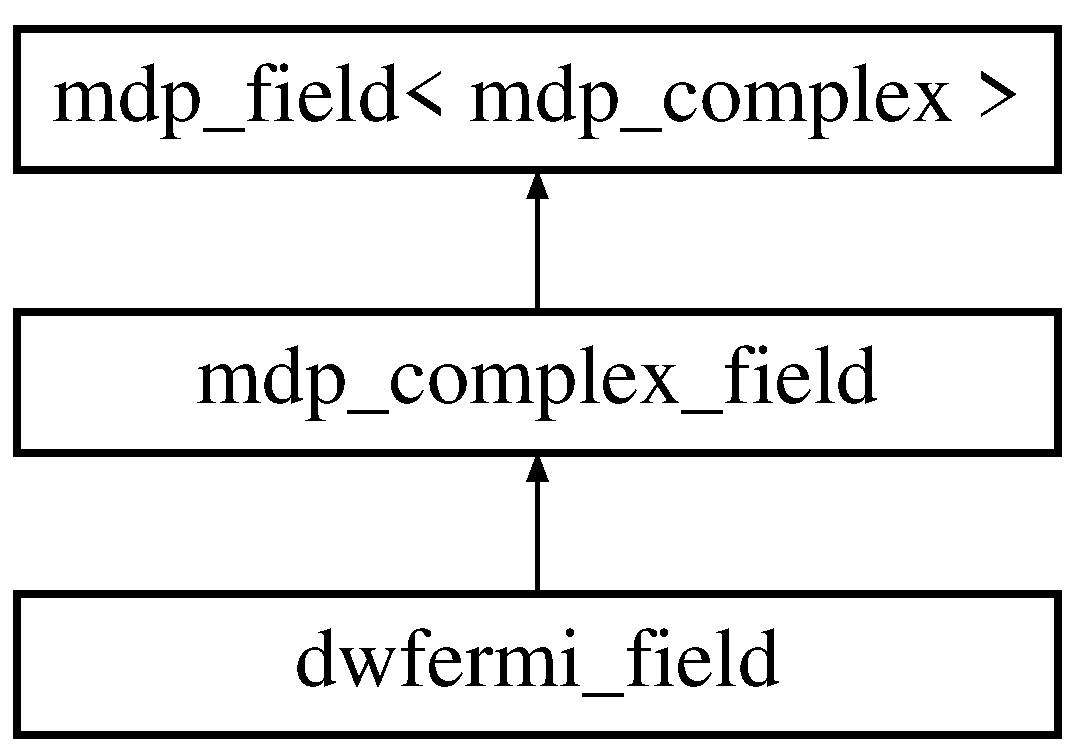
\includegraphics[height=3cm]{classdwfermi__field}
\end{center}
\end{figure}
\subsection*{Public Member Functions}
\begin{DoxyCompactItemize}
\item 
\hyperlink{classdwfermi__field_a3463b5fdc91d928f765eb4ee35601672}{dwfermi\_\-field} ()
\item 
\hyperlink{classdwfermi__field_aea31f2beacd9fbf84b10488566a63982}{dwfermi\_\-field} (\hyperlink{classmdp__lattice}{mdp\_\-lattice} \&a, int L5\_\-, int nc\_\-, int nspin\_\-=4)
\item 
\hyperlink{classdwfermi__field_ae761300ce0a04ef58386ca3e58c7311c}{dwfermi\_\-field} (const \hyperlink{classdwfermi__field}{dwfermi\_\-field} \&psi)
\item 
void \hyperlink{classdwfermi__field_ab1e90f60aff705fd67fe54265511359c}{allocate\_\-dwfermi\_\-field} (\hyperlink{classmdp__lattice}{mdp\_\-lattice} \&a, int L5\_\-, int nc\_\-, int nspin\_\-=4)
\item 
\hyperlink{classmdp__matrix}{mdp\_\-matrix} \hyperlink{classdwfermi__field_a74ca9ee1a200f082bf816a306e0db58a}{operator()} (site x, int L5\_\-)
\item 
\hyperlink{classmdp__matrix}{mdp\_\-matrix} \hyperlink{classdwfermi__field_adca7e6c16994ace10946016d8d6de943}{operator()} (site x, int L5\_\-, int a)
\item 
\hyperlink{classmdp__complex}{mdp\_\-complex} \& \hyperlink{classdwfermi__field_ac0d1e75f5248ce12c06e7fcb8add5948}{operator()} (site x, int L5\_\-, int a, int i)
\item 
const \hyperlink{classmdp__complex}{mdp\_\-complex} \& \hyperlink{classdwfermi__field_a38dcacb8755165fdfcb41622912f1863}{operator()} (site x, int L5\_\-, int a, int i) const 
\item 
void \hyperlink{classdwfermi__field_a80684935337a1c336bd81379787ba9f4}{operator=} (\hyperlink{classmdp__complex}{mdp\_\-complex} a)
\end{DoxyCompactItemize}
\subsection*{Public Attributes}
\begin{DoxyCompactItemize}
\item 
int \hyperlink{classdwfermi__field_ac56aca6bd128b92467fdf7dca86535aa}{nspin}
\item 
int \hyperlink{classdwfermi__field_ab4c38d0b9f1016a5b121eced43a19370}{nc}
\item 
int \hyperlink{classdwfermi__field_a8bb8d2f33c7060b39da0563969b712a9}{L5}
\end{DoxyCompactItemize}


\subsection{Detailed Description}
domain wall fermionic field Example: \begin{DoxyVerb}
/// int L5=10; // size in 5th dimension 
/// fermi_field psi(lattice,L5,nc);
/// mdp_site x(lattice);
/// forallsites(x)
///    for(int k=0; k<L5; k++)
///      for(int spin=0; spin<4; spin++)
///        for(int i=0; i<nc; i++)
///          psi(x,k,spin,i)=0.0+0.0*I;
/// \end{DoxyVerb}
 

\subsection{Constructor \& Destructor Documentation}
\hypertarget{classdwfermi__field_a3463b5fdc91d928f765eb4ee35601672}{
\index{dwfermi\_\-field@{dwfermi\_\-field}!dwfermi\_\-field@{dwfermi\_\-field}}
\index{dwfermi\_\-field@{dwfermi\_\-field}!dwfermi_field@{dwfermi\_\-field}}
\subsubsection[{dwfermi\_\-field}]{\setlength{\rightskip}{0pt plus 5cm}dwfermi\_\-field::dwfermi\_\-field ()\hspace{0.3cm}{\ttfamily  \mbox{[}inline\mbox{]}}}}
\label{classdwfermi__field_a3463b5fdc91d928f765eb4ee35601672}
\hypertarget{classdwfermi__field_aea31f2beacd9fbf84b10488566a63982}{
\index{dwfermi\_\-field@{dwfermi\_\-field}!dwfermi\_\-field@{dwfermi\_\-field}}
\index{dwfermi\_\-field@{dwfermi\_\-field}!dwfermi_field@{dwfermi\_\-field}}
\subsubsection[{dwfermi\_\-field}]{\setlength{\rightskip}{0pt plus 5cm}dwfermi\_\-field::dwfermi\_\-field ({\bf mdp\_\-lattice} \& {\em a}, \/  int {\em L5\_\-}, \/  int {\em nc\_\-}, \/  int {\em nspin\_\-} = {\ttfamily 4})\hspace{0.3cm}{\ttfamily  \mbox{[}inline\mbox{]}}}}
\label{classdwfermi__field_aea31f2beacd9fbf84b10488566a63982}
\hypertarget{classdwfermi__field_ae761300ce0a04ef58386ca3e58c7311c}{
\index{dwfermi\_\-field@{dwfermi\_\-field}!dwfermi\_\-field@{dwfermi\_\-field}}
\index{dwfermi\_\-field@{dwfermi\_\-field}!dwfermi_field@{dwfermi\_\-field}}
\subsubsection[{dwfermi\_\-field}]{\setlength{\rightskip}{0pt plus 5cm}dwfermi\_\-field::dwfermi\_\-field (const {\bf dwfermi\_\-field} \& {\em psi})\hspace{0.3cm}{\ttfamily  \mbox{[}inline\mbox{]}}}}
\label{classdwfermi__field_ae761300ce0a04ef58386ca3e58c7311c}


\subsection{Member Function Documentation}
\hypertarget{classdwfermi__field_ab1e90f60aff705fd67fe54265511359c}{
\index{dwfermi\_\-field@{dwfermi\_\-field}!allocate\_\-dwfermi\_\-field@{allocate\_\-dwfermi\_\-field}}
\index{allocate\_\-dwfermi\_\-field@{allocate\_\-dwfermi\_\-field}!dwfermi_field@{dwfermi\_\-field}}
\subsubsection[{allocate\_\-dwfermi\_\-field}]{\setlength{\rightskip}{0pt plus 5cm}void dwfermi\_\-field::allocate\_\-dwfermi\_\-field ({\bf mdp\_\-lattice} \& {\em a}, \/  int {\em L5\_\-}, \/  int {\em nc\_\-}, \/  int {\em nspin\_\-} = {\ttfamily 4})\hspace{0.3cm}{\ttfamily  \mbox{[}inline\mbox{]}}}}
\label{classdwfermi__field_ab1e90f60aff705fd67fe54265511359c}
\hypertarget{classdwfermi__field_a38dcacb8755165fdfcb41622912f1863}{
\index{dwfermi\_\-field@{dwfermi\_\-field}!operator()@{operator()}}
\index{operator()@{operator()}!dwfermi_field@{dwfermi\_\-field}}
\subsubsection[{operator()}]{\setlength{\rightskip}{0pt plus 5cm}const {\bf mdp\_\-complex}\& dwfermi\_\-field::operator() (site {\em x}, \/  int {\em L5\_\-}, \/  int {\em a}, \/  int {\em i}) const\hspace{0.3cm}{\ttfamily  \mbox{[}inline\mbox{]}}}}
\label{classdwfermi__field_a38dcacb8755165fdfcb41622912f1863}
\hypertarget{classdwfermi__field_ac0d1e75f5248ce12c06e7fcb8add5948}{
\index{dwfermi\_\-field@{dwfermi\_\-field}!operator()@{operator()}}
\index{operator()@{operator()}!dwfermi_field@{dwfermi\_\-field}}
\subsubsection[{operator()}]{\setlength{\rightskip}{0pt plus 5cm}{\bf mdp\_\-complex}\& dwfermi\_\-field::operator() (site {\em x}, \/  int {\em L5\_\-}, \/  int {\em a}, \/  int {\em i})\hspace{0.3cm}{\ttfamily  \mbox{[}inline\mbox{]}}}}
\label{classdwfermi__field_ac0d1e75f5248ce12c06e7fcb8add5948}
\hypertarget{classdwfermi__field_adca7e6c16994ace10946016d8d6de943}{
\index{dwfermi\_\-field@{dwfermi\_\-field}!operator()@{operator()}}
\index{operator()@{operator()}!dwfermi_field@{dwfermi\_\-field}}
\subsubsection[{operator()}]{\setlength{\rightskip}{0pt plus 5cm}{\bf mdp\_\-matrix} dwfermi\_\-field::operator() (site {\em x}, \/  int {\em L5\_\-}, \/  int {\em a})\hspace{0.3cm}{\ttfamily  \mbox{[}inline\mbox{]}}}}
\label{classdwfermi__field_adca7e6c16994ace10946016d8d6de943}
\hypertarget{classdwfermi__field_a74ca9ee1a200f082bf816a306e0db58a}{
\index{dwfermi\_\-field@{dwfermi\_\-field}!operator()@{operator()}}
\index{operator()@{operator()}!dwfermi_field@{dwfermi\_\-field}}
\subsubsection[{operator()}]{\setlength{\rightskip}{0pt plus 5cm}{\bf mdp\_\-matrix} dwfermi\_\-field::operator() (site {\em x}, \/  int {\em L5\_\-})\hspace{0.3cm}{\ttfamily  \mbox{[}inline\mbox{]}}}}
\label{classdwfermi__field_a74ca9ee1a200f082bf816a306e0db58a}
\hypertarget{classdwfermi__field_a80684935337a1c336bd81379787ba9f4}{
\index{dwfermi\_\-field@{dwfermi\_\-field}!operator=@{operator=}}
\index{operator=@{operator=}!dwfermi_field@{dwfermi\_\-field}}
\subsubsection[{operator=}]{\setlength{\rightskip}{0pt plus 5cm}void dwfermi\_\-field::operator= ({\bf mdp\_\-complex} {\em a})\hspace{0.3cm}{\ttfamily  \mbox{[}inline\mbox{]}}}}
\label{classdwfermi__field_a80684935337a1c336bd81379787ba9f4}


Reimplemented from \hyperlink{classmdp__field_a24364bce6444668661a0688632af87ec}{mdp\_\-field$<$ mdp\_\-complex $>$}.

\subsection{Member Data Documentation}
\hypertarget{classdwfermi__field_a8bb8d2f33c7060b39da0563969b712a9}{
\index{dwfermi\_\-field@{dwfermi\_\-field}!L5@{L5}}
\index{L5@{L5}!dwfermi_field@{dwfermi\_\-field}}
\subsubsection[{L5}]{\setlength{\rightskip}{0pt plus 5cm}int {\bf dwfermi\_\-field::L5}}}
\label{classdwfermi__field_a8bb8d2f33c7060b39da0563969b712a9}
\hypertarget{classdwfermi__field_ab4c38d0b9f1016a5b121eced43a19370}{
\index{dwfermi\_\-field@{dwfermi\_\-field}!nc@{nc}}
\index{nc@{nc}!dwfermi_field@{dwfermi\_\-field}}
\subsubsection[{nc}]{\setlength{\rightskip}{0pt plus 5cm}int {\bf dwfermi\_\-field::nc}}}
\label{classdwfermi__field_ab4c38d0b9f1016a5b121eced43a19370}
\hypertarget{classdwfermi__field_ac56aca6bd128b92467fdf7dca86535aa}{
\index{dwfermi\_\-field@{dwfermi\_\-field}!nspin@{nspin}}
\index{nspin@{nspin}!dwfermi_field@{dwfermi\_\-field}}
\subsubsection[{nspin}]{\setlength{\rightskip}{0pt plus 5cm}int {\bf dwfermi\_\-field::nspin}}}
\label{classdwfermi__field_ac56aca6bd128b92467fdf7dca86535aa}


The documentation for this class was generated from the following file:\begin{DoxyCompactItemize}
\item 
/Users/mdipierro/fermiqcd/development/Libraries/\hyperlink{fermiqcd__dwfermi__field_8h}{fermiqcd\_\-dwfermi\_\-field.h}\end{DoxyCompactItemize}

\hypertarget{class_d_w_fermi_action_fast}{
\section{DWFermiActionFast Class Reference}
\label{class_d_w_fermi_action_fast}\index{DWFermiActionFast@{DWFermiActionFast}}
}


domain wall action fast  


{\ttfamily \#include $<$fermiqcd\_\-dwfermi\_\-actions.h$>$}\subsection*{Static Public Member Functions}
\begin{DoxyCompactItemize}
\item 
static void \hyperlink{class_d_w_fermi_action_fast_a52079bb2144dc7ef2f61c4916f9569ca}{mul\_\-Q} (\hyperlink{classdwfermi__field}{dwfermi\_\-field} \&psi\_\-out, \hyperlink{classdwfermi__field}{dwfermi\_\-field} \&psi\_\-in, \hyperlink{classgauge__field}{gauge\_\-field} \&U, \hyperlink{classcoefficients}{coefficients} \&coeff)
\end{DoxyCompactItemize}


\subsection{Detailed Description}
domain wall action fast Notation from ref. hep-\/lat/0007038 Example: \begin{DoxyVerb}
/// gauge_field U(lattice,nc);
/// dwfermi_field psi(lattice,nc);
/// dwfermi_field chi(lattice,nc);
/// coefficients coeff;
/// coeff["m_f"]=0.11; // fermion mass
/// coeff["m_5"]=0.11; // mass in 5th dimension
/// default_dwfermi_action=DWFermiActionFast::mul_Q;
/// mul_Q(chi,psi,U,coeff);
/// \end{DoxyVerb}
 Note that mul\_\-Q(chi,psi,U,coeff) reads $ \chi=(/\!\!\!D[U]+m)\psi $ 

\subsection{Member Function Documentation}
\hypertarget{class_d_w_fermi_action_fast_a52079bb2144dc7ef2f61c4916f9569ca}{
\index{DWFermiActionFast@{DWFermiActionFast}!mul\_\-Q@{mul\_\-Q}}
\index{mul\_\-Q@{mul\_\-Q}!DWFermiActionFast@{DWFermiActionFast}}
\subsubsection[{mul\_\-Q}]{\setlength{\rightskip}{0pt plus 5cm}static void DWFermiActionFast::mul\_\-Q ({\bf dwfermi\_\-field} \& {\em psi\_\-out}, \/  {\bf dwfermi\_\-field} \& {\em psi\_\-in}, \/  {\bf gauge\_\-field} \& {\em U}, \/  {\bf coefficients} \& {\em coeff})\hspace{0.3cm}{\ttfamily  \mbox{[}inline, static\mbox{]}}}}
\label{class_d_w_fermi_action_fast_a52079bb2144dc7ef2f61c4916f9569ca}


The documentation for this class was generated from the following file:\begin{DoxyCompactItemize}
\item 
/Users/mdipierro/fermiqcd/development/Libraries/\hyperlink{fermiqcd__dwfermi__actions_8h}{fermiqcd\_\-dwfermi\_\-actions.h}\end{DoxyCompactItemize}

\hypertarget{class_d_w_fermi_action_slow}{
\section{DWFermiActionSlow Class Reference}
\label{class_d_w_fermi_action_slow}\index{DWFermiActionSlow@{DWFermiActionSlow}}
}
domain wall action (SORRY THIS IS SLOW)  


{\tt \#include $<$fermiqcd\_\-dwfermi\_\-actions.h$>$}



\subsection{Detailed Description}
domain wall action (SORRY THIS IS SLOW) 

Notation from ref. hep-lat/0007038 Example: 

\footnotesize\begin{verbatim}
/// gauge_field U(lattice,nc);
/// dwfermi_field psi(lattice,nc);
/// dwfermi_field chi(lattice,nc);
/// coefficients coeff;
/// coeff["m_f"]=0.11; // fermion mass
/// coeff["m_5"]=0.11; // mass in 5th dimension
/// default_dwfermi_action=DWFermiActionSlow::mul_Q;
/// mul_Q(chi,psi,U,coeff);
/// \end{verbatim}
\normalsize
 Note that mul\_\-Q(chi,psi,U,coeff) reads $ \chi=(/\!\!\!D[U]+m)\psi $ 

The documentation for this class was generated from the following file:\begin{CompactItemize}
\item 
/Users/mdipierro/Desktop/SciDac/development/Libraries/\hyperlink{fermiqcd__dwfermi__actions_8h}{fermiqcd\_\-dwfermi\_\-actions.h}\end{CompactItemize}

\hypertarget{classem__field}{
\section{em\_\-field Class Reference}
\label{classem__field}\index{em\_\-field@{em\_\-field}}
}
the chromo-electr-magnetic field for any SU(n)  


{\tt \#include $<$fermiqcd\_\-gauge\_\-field.h$>$}

Inherits \hyperlink{classmdp__complex__field}{mdp\_\-complex\_\-field}.

Collaboration diagram for em\_\-field:

\subsection{Detailed Description}
the chromo-electr-magnetic field for any SU(n) 

Example: 

\footnotesize\begin{verbatim}
///    int nc=3; 
///    int box[]={10,8,8,8};
///    mdp_lattice lattice(4,box);
///    gauge_field U(lattice,nc);
///    mdp_site x(lattice);
///    U.load("myfield");
///    compute_em_field(U);
///    forallsites(x)
///      for(int mu=0; mu<U.ndim; mu++)
///        for(int nu=mu+1; nu<U.ndim; nu++)
///          cout << U.em(x,mu,nu) << endl;
/// \end{verbatim}
\normalsize
 Note that U.em(x,mu,nu) is $ a^2 G_{\mu\nu} $ and it is a color matrix in SU(nc). $a$ is the lattice spacing. 

The documentation for this class was generated from the following file:\begin{CompactItemize}
\item 
/Users/mdipierro/Desktop/SciDac/development/Libraries/\hyperlink{fermiqcd__gauge__field_8h}{fermiqcd\_\-gauge\_\-field.h}\end{CompactItemize}

\hypertarget{classfermi__field}{
\section{fermi\_\-field Class Reference}
\label{classfermi__field}\index{fermi\_\-field@{fermi\_\-field}}
}
wilson fermionic field  


{\tt \#include $<$fermiqcd\_\-fermi\_\-field.h$>$}

Inherits \hyperlink{classmdp__complex__field}{mdp\_\-complex\_\-field}.

Collaboration diagram for fermi\_\-field:

\subsection{Detailed Description}
wilson fermionic field 

Example: 

\footnotesize\begin{verbatim}
/// fermi_field psi(lattice,nc);
/// mdp_site x(lattice);
/// forallsites(x)
///    for(int spin=0; spin<4; spin++)
///      for(int i=0; i<nc; i++)
///        psi(x,spin,i)=0.0+0.0*I;
/// \end{verbatim}
\normalsize
 

The documentation for this class was generated from the following file:\begin{CompactItemize}
\item 
/Users/mdipierro/Desktop/SciDac/development/Libraries/\hyperlink{fermiqcd__fermi__field_8h}{fermiqcd\_\-fermi\_\-field.h}\end{CompactItemize}

\hypertarget{classfermi__propagator}{
\section{fermi\_\-propagator Class Reference}
\label{classfermi__propagator}\index{fermi\_\-propagator@{fermi\_\-propagator}}
}


a Wilson/Clover quark propagator (all 12 components)  


{\ttfamily \#include $<$fermiqcd\_\-fermi\_\-propagator.h$>$}Inheritance diagram for fermi\_\-propagator::\begin{figure}[H]
\begin{center}
\leavevmode
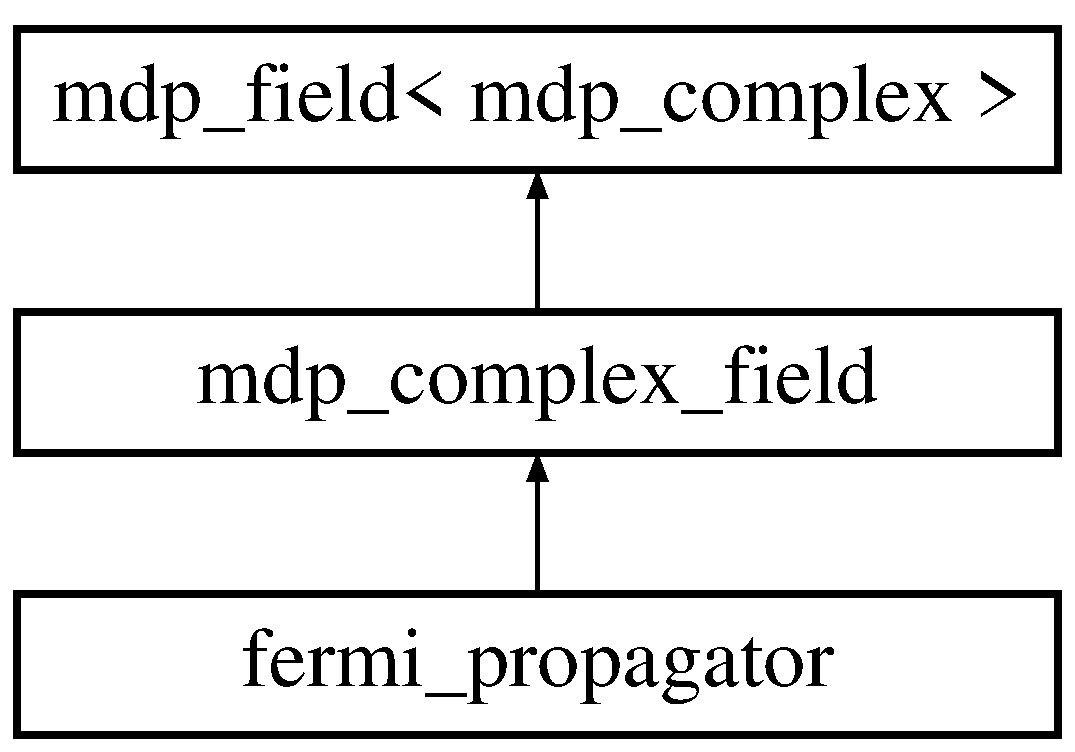
\includegraphics[height=3cm]{classfermi__propagator}
\end{center}
\end{figure}
\subsection*{Public Member Functions}
\begin{DoxyCompactItemize}
\item 
\hyperlink{classfermi__propagator_a55bbd357d5ffd3b57f835dab4a06d261}{fermi\_\-propagator} ()
\item 
\hyperlink{classfermi__propagator_a41b0242793ca3da9ec2e67cdc05a9149}{fermi\_\-propagator} (\hyperlink{classmdp__lattice}{mdp\_\-lattice} \&mylattice, int nc\_\-, int nspin\_\-=4)
\item 
void \hyperlink{classfermi__propagator_a8ee1c8631f83f4e4876eff6253c41954}{allocate\_\-fermi\_\-propagator} (\hyperlink{classmdp__lattice}{mdp\_\-lattice} \&mylattice, int nc\_\-, int nspin\_\-=4)
\item 
\hyperlink{classmdp__matrix}{mdp\_\-matrix} \hyperlink{classfermi__propagator_afb016830eaa4959a21901d5895adb4bc}{operator()} (site x, int a, int b)
\item 
\hyperlink{classmdp__complex}{mdp\_\-complex} \& \hyperlink{classfermi__propagator_a8552fbd45ff1fd6b450353713dc21bcd}{operator()} (site x, int a, int b, int i, int j)
\end{DoxyCompactItemize}
\subsection*{Public Attributes}
\begin{DoxyCompactItemize}
\item 
int \hyperlink{classfermi__propagator_a5eae6edf77379e878f84281aa9e32316}{nspin}
\item 
int \hyperlink{classfermi__propagator_a75d862433489db5a07b2ced97c21f9cc}{nc}
\end{DoxyCompactItemize}
\subsection*{Friends}
\begin{DoxyCompactItemize}
\item 
void \hyperlink{classfermi__propagator_a0b3730ff1e1058f1e13b537d429c7333}{generate} (\hyperlink{classfermi__propagator}{fermi\_\-propagator} \&S, \hyperlink{classgauge__field}{gauge\_\-field} \&U, \hyperlink{classcoefficients}{coefficients} \&coeff, \hyperlink{mdp__global__vars_8h_a049e4c1d4e74d644878a42f9909463e4}{mdp\_\-real} absolute\_\-precision=\hyperlink{fermiqcd__default__parameters_8h_ab11c95dc923c6bfd349bd67af277d59d}{fermi\_\-inversion\_\-precision}, \hyperlink{mdp__global__vars_8h_a049e4c1d4e74d644878a42f9909463e4}{mdp\_\-real} relative\_\-precision=0, int max\_\-steps=2000, void($\ast$smf)(\hyperlink{classfermi__field}{fermi\_\-field} \&, \hyperlink{classgauge__field}{gauge\_\-field} \&, \hyperlink{classcoefficients}{coefficients} \&)=0, \hyperlink{classcoefficients}{coefficients} smear\_\-coeff=\hyperlink{classcoefficients}{coefficients}(), int comp=0)
\end{DoxyCompactItemize}


\subsection{Detailed Description}
a Wilson/Clover quark propagator (all 12 components) Example of how to make a pion: \begin{DoxyVerb}
/// gauge_field U(lattice,nc);
/// U.load("myfield");
/// fermi_propagator S(lattice,nc);
/// coefficients quark;
/// quark["kappa"]=1.12;
/// generate(S,U,quark);
/// vector<float> sum(U.lattice.size(TIME));
/// forallsites(x) 
///   for(int alpha=0; alpha<4; alpha++)
///     for(int beta=0; beta<4; beta++)
///        sum(x(0))+=real(trace(S(x,alpha,beta)*
///                   hermitian(S(x,beta,alpha))));
/// \end{DoxyVerb}
 Note that S(x,alpha,beta,i,j) is $ \left<0|\bar q^i_\alpha(x), q^j_\beta(0)|\right> $ 

\subsection{Constructor \& Destructor Documentation}
\hypertarget{classfermi__propagator_a55bbd357d5ffd3b57f835dab4a06d261}{
\index{fermi\_\-propagator@{fermi\_\-propagator}!fermi\_\-propagator@{fermi\_\-propagator}}
\index{fermi\_\-propagator@{fermi\_\-propagator}!fermi_propagator@{fermi\_\-propagator}}
\subsubsection[{fermi\_\-propagator}]{\setlength{\rightskip}{0pt plus 5cm}fermi\_\-propagator::fermi\_\-propagator ()\hspace{0.3cm}{\ttfamily  \mbox{[}inline\mbox{]}}}}
\label{classfermi__propagator_a55bbd357d5ffd3b57f835dab4a06d261}
\hypertarget{classfermi__propagator_a41b0242793ca3da9ec2e67cdc05a9149}{
\index{fermi\_\-propagator@{fermi\_\-propagator}!fermi\_\-propagator@{fermi\_\-propagator}}
\index{fermi\_\-propagator@{fermi\_\-propagator}!fermi_propagator@{fermi\_\-propagator}}
\subsubsection[{fermi\_\-propagator}]{\setlength{\rightskip}{0pt plus 5cm}fermi\_\-propagator::fermi\_\-propagator ({\bf mdp\_\-lattice} \& {\em mylattice}, \/  int {\em nc\_\-}, \/  int {\em nspin\_\-} = {\ttfamily 4})\hspace{0.3cm}{\ttfamily  \mbox{[}inline\mbox{]}}}}
\label{classfermi__propagator_a41b0242793ca3da9ec2e67cdc05a9149}


\subsection{Member Function Documentation}
\hypertarget{classfermi__propagator_a8ee1c8631f83f4e4876eff6253c41954}{
\index{fermi\_\-propagator@{fermi\_\-propagator}!allocate\_\-fermi\_\-propagator@{allocate\_\-fermi\_\-propagator}}
\index{allocate\_\-fermi\_\-propagator@{allocate\_\-fermi\_\-propagator}!fermi_propagator@{fermi\_\-propagator}}
\subsubsection[{allocate\_\-fermi\_\-propagator}]{\setlength{\rightskip}{0pt plus 5cm}void fermi\_\-propagator::allocate\_\-fermi\_\-propagator ({\bf mdp\_\-lattice} \& {\em mylattice}, \/  int {\em nc\_\-}, \/  int {\em nspin\_\-} = {\ttfamily 4})\hspace{0.3cm}{\ttfamily  \mbox{[}inline\mbox{]}}}}
\label{classfermi__propagator_a8ee1c8631f83f4e4876eff6253c41954}
\hypertarget{classfermi__propagator_a8552fbd45ff1fd6b450353713dc21bcd}{
\index{fermi\_\-propagator@{fermi\_\-propagator}!operator()@{operator()}}
\index{operator()@{operator()}!fermi_propagator@{fermi\_\-propagator}}
\subsubsection[{operator()}]{\setlength{\rightskip}{0pt plus 5cm}{\bf mdp\_\-complex}\& fermi\_\-propagator::operator() (site {\em x}, \/  int {\em a}, \/  int {\em b}, \/  int {\em i}, \/  int {\em j})\hspace{0.3cm}{\ttfamily  \mbox{[}inline\mbox{]}}}}
\label{classfermi__propagator_a8552fbd45ff1fd6b450353713dc21bcd}
\hypertarget{classfermi__propagator_afb016830eaa4959a21901d5895adb4bc}{
\index{fermi\_\-propagator@{fermi\_\-propagator}!operator()@{operator()}}
\index{operator()@{operator()}!fermi_propagator@{fermi\_\-propagator}}
\subsubsection[{operator()}]{\setlength{\rightskip}{0pt plus 5cm}{\bf mdp\_\-matrix} fermi\_\-propagator::operator() (site {\em x}, \/  int {\em a}, \/  int {\em b})\hspace{0.3cm}{\ttfamily  \mbox{[}inline\mbox{]}}}}
\label{classfermi__propagator_afb016830eaa4959a21901d5895adb4bc}


\subsection{Friends And Related Function Documentation}
\hypertarget{classfermi__propagator_a0b3730ff1e1058f1e13b537d429c7333}{
\index{fermi\_\-propagator@{fermi\_\-propagator}!generate@{generate}}
\index{generate@{generate}!fermi_propagator@{fermi\_\-propagator}}
\subsubsection[{generate}]{\setlength{\rightskip}{0pt plus 5cm}void generate ({\bf fermi\_\-propagator} \& {\em S}, \/  {\bf gauge\_\-field} \& {\em U}, \/  {\bf coefficients} \& {\em coeff}, \/  {\bf mdp\_\-real} {\em absolute\_\-precision} = {\ttfamily {\bf fermi\_\-inversion\_\-precision}}, \/  {\bf mdp\_\-real} {\em relative\_\-precision} = {\ttfamily 0}, \/  int {\em max\_\-steps} = {\ttfamily 2000}, \/  void($\ast$)({\bf fermi\_\-field} \&, {\bf gauge\_\-field} \&, {\bf coefficients} \&) {\em smf} = {\ttfamily 0}, \/  {\bf coefficients} {\em smear\_\-coeff} = {\ttfamily {\bf coefficients}()}, \/  int {\em comp} = {\ttfamily 0})\hspace{0.3cm}{\ttfamily  \mbox{[}friend\mbox{]}}}}
\label{classfermi__propagator_a0b3730ff1e1058f1e13b537d429c7333}
makes the quark propagator


\begin{DoxyParams}{Parameters}
\item[{\em S}]the output propagator \item[{\em U}]the input gauge configuration \item[{\em coeff}]the parameters to be passed to the action \item[{\em absolute\_\-precision}]the target absolute precision for inversion \item[{\em relative\_\-precision}]the target relative precision for invcersion \item[{\em max\_\-steps}]the max number of steps in inversion \item[{\em smf}]pointer to smearing function (smear sources) \item[{\em smear\_\-coeff}]parameters for smearing \end{DoxyParams}


\subsection{Member Data Documentation}
\hypertarget{classfermi__propagator_a75d862433489db5a07b2ced97c21f9cc}{
\index{fermi\_\-propagator@{fermi\_\-propagator}!nc@{nc}}
\index{nc@{nc}!fermi_propagator@{fermi\_\-propagator}}
\subsubsection[{nc}]{\setlength{\rightskip}{0pt plus 5cm}int {\bf fermi\_\-propagator::nc}}}
\label{classfermi__propagator_a75d862433489db5a07b2ced97c21f9cc}
\hypertarget{classfermi__propagator_a5eae6edf77379e878f84281aa9e32316}{
\index{fermi\_\-propagator@{fermi\_\-propagator}!nspin@{nspin}}
\index{nspin@{nspin}!fermi_propagator@{fermi\_\-propagator}}
\subsubsection[{nspin}]{\setlength{\rightskip}{0pt plus 5cm}int {\bf fermi\_\-propagator::nspin}}}
\label{classfermi__propagator_a5eae6edf77379e878f84281aa9e32316}


The documentation for this class was generated from the following file:\begin{DoxyCompactItemize}
\item 
/Users/mdipierro/fermiqcd/development/Libraries/\hyperlink{fermiqcd__fermi__propagator_8h}{fermiqcd\_\-fermi\_\-propagator.h}\end{DoxyCompactItemize}

\hypertarget{class_fermi_clover_action_fast}{
\section{FermiCloverActionFast Class Reference}
\label{class_fermi_clover_action_fast}\index{FermiCloverActionFast@{FermiCloverActionFast}}
}
Wilson/Clover action.  


{\tt \#include $<$fermiqcd\_\-fermi\_\-actions.h$>$}



\subsection{Detailed Description}
Wilson/Clover action. 

Example: 

\footnotesize\begin{verbatim}
/// gauge_field U(lattice,nc);
/// fermi_field psi(lattice,nc);
/// fermi_field chi(lattice,nc);
/// coefficients coeff;
/// coeff["kappa_s"]=0.11;
/// coeff["kappa_t"]=0.11;
/// coeff["r_s"]=1.0;
/// coeff["r_t"]=1.0;
/// coeff["c_{sw}"]=1.0;
/// coeff["c_E"]=1.0;
/// coeff["c_B"]=1.0;
/// default_fermi_action=FermiCloverActionFast::mul_Q;
/// if(coeff["c_{sw}"]!=0) compute_em_field(U);
/// mul_Q(chi,psi,U,coeff);
/// \end{verbatim}
\normalsize
 

The documentation for this class was generated from the following file:\begin{CompactItemize}
\item 
/Users/mdipierro/Desktop/SciDac/development/Libraries/\hyperlink{fermiqcd__fermi__actions_8h}{fermiqcd\_\-fermi\_\-actions.h}\end{CompactItemize}

\hypertarget{class_fermi_clover_action_slow}{
\section{FermiCloverActionSlow Class Reference}
\label{class_fermi_clover_action_slow}\index{FermiCloverActionSlow@{FermiCloverActionSlow}}
}


Wilson/Clover action (SLOW: DO NOT USE IN PRODUCTION).  


{\ttfamily \#include $<$fermiqcd\_\-fermi\_\-actions.h$>$}\subsection*{Static Public Member Functions}
\begin{DoxyCompactItemize}
\item 
static void \hyperlink{class_fermi_clover_action_slow_a8e9b281981e3907873fc08c52f2c3d21}{mul\_\-Q} (\hyperlink{classfermi__field}{fermi\_\-field} \&psi\_\-out, \hyperlink{classfermi__field}{fermi\_\-field} \&psi\_\-in, \hyperlink{classgauge__field}{gauge\_\-field} \&U, \hyperlink{classcoefficients}{coefficients} \&coeff, int parity=\hyperlink{mdp__global__vars_8h_a4c9de81f2de5a74b588107b6c0afb9ee}{EVENODD})
\end{DoxyCompactItemize}


\subsection{Detailed Description}
Wilson/Clover action (SLOW: DO NOT USE IN PRODUCTION). Example: \begin{DoxyVerb}
/// gauge_field U(lattice,nc);
/// fermi_field psi(lattice,nc);
/// fermi_field chi(lattice,nc);
/// coefficients coeff;
/// coeff["kappa_s"]=0.11;
/// coeff["kappa_t"]=0.11;
/// coeff["r_s"]=1.0;
/// coeff["r_t"]=1.0;
/// coeff["c_{sw}"]=1.0;
/// coeff["c_E"]=1.0;
/// coeff["c_B"]=1.0;
/// default_fermi_action=FermiCloverActionSlow::mul_Q;
/// if(coeff["c_{sw}"]!=0) compute_em_field(U);
/// mul_Q(chi,psi,U,coeff);
/// \end{DoxyVerb}
 Note that mul\_\-Q(chi,psi,U,coeff) reads $ \chi=(/\!\!\!D[U]+m)\psi $ 

\subsection{Member Function Documentation}
\hypertarget{class_fermi_clover_action_slow_a8e9b281981e3907873fc08c52f2c3d21}{
\index{FermiCloverActionSlow@{FermiCloverActionSlow}!mul\_\-Q@{mul\_\-Q}}
\index{mul\_\-Q@{mul\_\-Q}!FermiCloverActionSlow@{FermiCloverActionSlow}}
\subsubsection[{mul\_\-Q}]{\setlength{\rightskip}{0pt plus 5cm}static void FermiCloverActionSlow::mul\_\-Q ({\bf fermi\_\-field} \& {\em psi\_\-out}, \/  {\bf fermi\_\-field} \& {\em psi\_\-in}, \/  {\bf gauge\_\-field} \& {\em U}, \/  {\bf coefficients} \& {\em coeff}, \/  int {\em parity} = {\ttfamily {\bf EVENODD}})\hspace{0.3cm}{\ttfamily  \mbox{[}inline, static\mbox{]}}}}
\label{class_fermi_clover_action_slow_a8e9b281981e3907873fc08c52f2c3d21}


The documentation for this class was generated from the following file:\begin{DoxyCompactItemize}
\item 
/Users/mdipierro/fermiqcd/development/Libraries/\hyperlink{fermiqcd__fermi__actions_8h}{fermiqcd\_\-fermi\_\-actions.h}\end{DoxyCompactItemize}

\hypertarget{classgauge__field}{
\section{gauge\_\-field Class Reference}
\label{classgauge__field}\index{gauge\_\-field@{gauge\_\-field}}
}


the gauge field for any SU(n)  


{\ttfamily \#include $<$fermiqcd\_\-gauge\_\-field.h$>$}Inheritance diagram for gauge\_\-field::\begin{figure}[H]
\begin{center}
\leavevmode
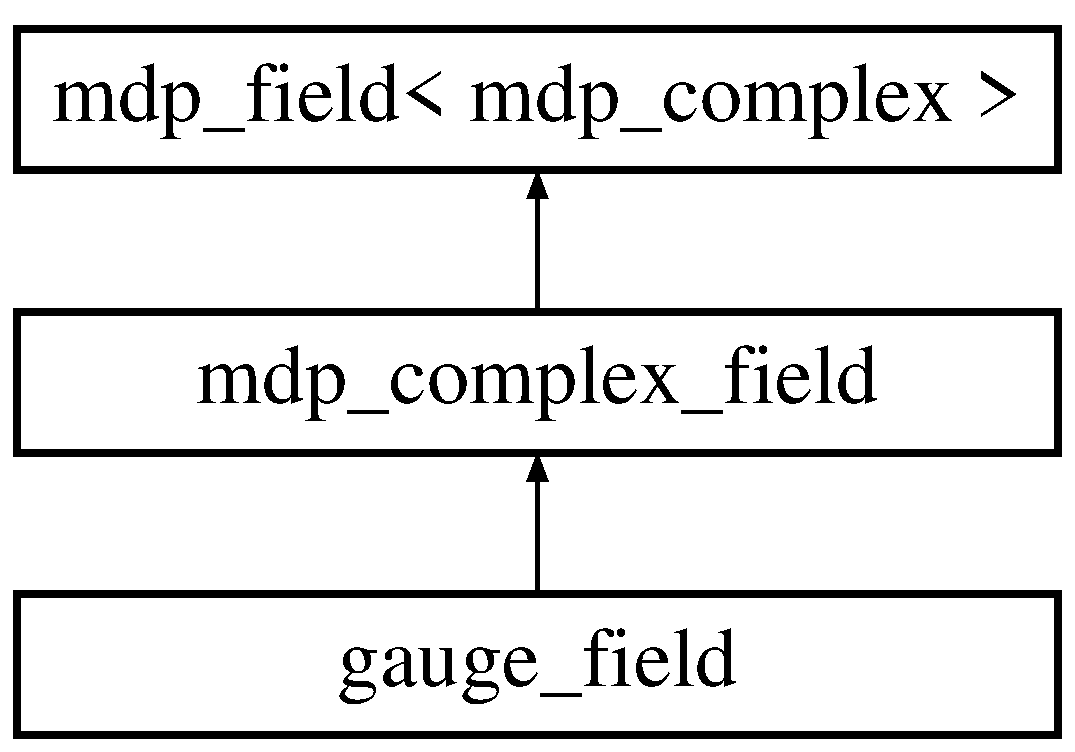
\includegraphics[height=3cm]{classgauge__field}
\end{center}
\end{figure}
\subsection*{Public Member Functions}
\begin{DoxyCompactItemize}
\item 
\hyperlink{classgauge__field_abdb50dfc413d1c22904a0ea38fc72e34}{gauge\_\-field} ()
\item 
\hyperlink{classgauge__field_a0500e23c8bd48d78650235e6ae668ab0}{gauge\_\-field} (const \hyperlink{classgauge__field}{gauge\_\-field} \&U)
\item 
void \hyperlink{classgauge__field_a1006054965a512e4dd06ca8c0b5c5d28}{operator=} (const \hyperlink{classgauge__field}{gauge\_\-field} \&U)
\item 
\hyperlink{classgauge__field_adcfa1a4c412dc26688307e95f3ed42b5}{gauge\_\-field} (\hyperlink{classmdp__lattice}{mdp\_\-lattice} \&a, int nc\_\-)
\item 
void \hyperlink{classgauge__field_ac7af990c989c01f0254a5454fc365dd7}{allocate\_\-gauge\_\-field} (\hyperlink{classmdp__lattice}{mdp\_\-lattice} \&a, int nc\_\-)
\item 
\hyperlink{classmdp__matrix}{mdp\_\-matrix} \hyperlink{classgauge__field_a765260519dece4a4ffafa338cbee22ae}{operator()} (site x, int mu)
\item 
const \hyperlink{classmdp__matrix}{mdp\_\-matrix} \hyperlink{classgauge__field_a8bbf9acb59886d8fcd08973476f224f6}{operator()} (site x, int mu) const 
\item 
\hyperlink{classmdp__complex}{mdp\_\-complex} \& \hyperlink{classgauge__field_a60a42ee4e59ad13f7bab46ba6f4ef2d9}{operator()} (site x, int mu, int i, int j)
\item 
const \hyperlink{classmdp__complex}{mdp\_\-complex} \& \hyperlink{classgauge__field_a3d76d90e8a6f39b0897cf463d6d8d049}{operator()} (site x, int mu, int i, int j) const 
\item 
\hyperlink{classmdp__matrix}{mdp\_\-matrix} \hyperlink{classgauge__field_a8d68963fa439cf58c3ac16c043523010}{operator()} (site x, int sign, int mu)
\item 
const \hyperlink{classmdp__matrix}{mdp\_\-matrix} \hyperlink{classgauge__field_afc4082b84abc10e1be05168c9898fddd}{operator()} (site x, int sign, int mu) const 
\item 
const \hyperlink{classmdp__complex}{mdp\_\-complex} \hyperlink{classgauge__field_a9dd484a3ca793d5e0376bbe2c2cd8995}{operator()} (site x, int sign, int mu, int i, int j) const 
\end{DoxyCompactItemize}
\subsection*{Public Attributes}
\begin{DoxyCompactItemize}
\item 
\hyperlink{classem__field}{em\_\-field} \hyperlink{classgauge__field_a8e12cc66b84dc51a33e0a942cc7c3f5c}{em}
\item 
\hyperlink{classmdp__nmatrix__field}{mdp\_\-nmatrix\_\-field} \hyperlink{classgauge__field_a2371b7cec512a57c18ba34269a5ba95a}{long\_\-links}
\item 
\hyperlink{classmdp__field}{mdp\_\-field}$<$ \hyperlink{mdp__global__vars_8h_aaa1ad9d0dcd2124aa5af0120d9954174}{mdp\_\-int} $>$ \hyperlink{classgauge__field_a3914ca4c0b33e495a2c1d34f158d6ce2}{i\_\-jump}
\item 
\hyperlink{classmdp__matrix__field}{mdp\_\-matrix\_\-field} \hyperlink{classgauge__field_a8b62d947d9237b33c554f3490cd62335}{swirls}
\item 
int \hyperlink{classgauge__field_a6be2d71c62063374567046e00cfb0983}{ndim}
\item 
int \hyperlink{classgauge__field_ada7f51e4041a64c45f484fc0a734a464}{nc}
\end{DoxyCompactItemize}


\subsection{Detailed Description}
the gauge field for any SU(n) Example: \begin{DoxyVerb}
///    int nc=3; 
///    int box[]={10,8,8,8};
///    mdp_lattice lattice(4,box);
///    gauge_field U(lattice,nc);
///    mdp_site x(lattice);
///    // set_cold(U);
///    forallsites(x)
///       for(int mu=0; mu<U.ndim; mu++)
///          U(x,mu)=1;
///    U.update(); // synchronization
///    U.save("myfield");
///    U.load("myfield");
/// \end{DoxyVerb}
 Note that U(x,mu) is $ \exp{iaA_{\mu}} $ and it is a color matrix in SU(nc). $a$ is the lattice spacing. 

\subsection{Constructor \& Destructor Documentation}
\hypertarget{classgauge__field_abdb50dfc413d1c22904a0ea38fc72e34}{
\index{gauge\_\-field@{gauge\_\-field}!gauge\_\-field@{gauge\_\-field}}
\index{gauge\_\-field@{gauge\_\-field}!gauge_field@{gauge\_\-field}}
\subsubsection[{gauge\_\-field}]{\setlength{\rightskip}{0pt plus 5cm}gauge\_\-field::gauge\_\-field ()\hspace{0.3cm}{\ttfamily  \mbox{[}inline\mbox{]}}}}
\label{classgauge__field_abdb50dfc413d1c22904a0ea38fc72e34}
\hypertarget{classgauge__field_a0500e23c8bd48d78650235e6ae668ab0}{
\index{gauge\_\-field@{gauge\_\-field}!gauge\_\-field@{gauge\_\-field}}
\index{gauge\_\-field@{gauge\_\-field}!gauge_field@{gauge\_\-field}}
\subsubsection[{gauge\_\-field}]{\setlength{\rightskip}{0pt plus 5cm}gauge\_\-field::gauge\_\-field (const {\bf gauge\_\-field} \& {\em U})\hspace{0.3cm}{\ttfamily  \mbox{[}inline\mbox{]}}}}
\label{classgauge__field_a0500e23c8bd48d78650235e6ae668ab0}
\hypertarget{classgauge__field_adcfa1a4c412dc26688307e95f3ed42b5}{
\index{gauge\_\-field@{gauge\_\-field}!gauge\_\-field@{gauge\_\-field}}
\index{gauge\_\-field@{gauge\_\-field}!gauge_field@{gauge\_\-field}}
\subsubsection[{gauge\_\-field}]{\setlength{\rightskip}{0pt plus 5cm}gauge\_\-field::gauge\_\-field ({\bf mdp\_\-lattice} \& {\em a}, \/  int {\em nc\_\-})\hspace{0.3cm}{\ttfamily  \mbox{[}inline\mbox{]}}}}
\label{classgauge__field_adcfa1a4c412dc26688307e95f3ed42b5}


\subsection{Member Function Documentation}
\hypertarget{classgauge__field_ac7af990c989c01f0254a5454fc365dd7}{
\index{gauge\_\-field@{gauge\_\-field}!allocate\_\-gauge\_\-field@{allocate\_\-gauge\_\-field}}
\index{allocate\_\-gauge\_\-field@{allocate\_\-gauge\_\-field}!gauge_field@{gauge\_\-field}}
\subsubsection[{allocate\_\-gauge\_\-field}]{\setlength{\rightskip}{0pt plus 5cm}void gauge\_\-field::allocate\_\-gauge\_\-field ({\bf mdp\_\-lattice} \& {\em a}, \/  int {\em nc\_\-})\hspace{0.3cm}{\ttfamily  \mbox{[}inline\mbox{]}}}}
\label{classgauge__field_ac7af990c989c01f0254a5454fc365dd7}
\hypertarget{classgauge__field_a9dd484a3ca793d5e0376bbe2c2cd8995}{
\index{gauge\_\-field@{gauge\_\-field}!operator()@{operator()}}
\index{operator()@{operator()}!gauge_field@{gauge\_\-field}}
\subsubsection[{operator()}]{\setlength{\rightskip}{0pt plus 5cm}const {\bf mdp\_\-complex} gauge\_\-field::operator() (site {\em x}, \/  int {\em sign}, \/  int {\em mu}, \/  int {\em i}, \/  int {\em j}) const\hspace{0.3cm}{\ttfamily  \mbox{[}inline\mbox{]}}}}
\label{classgauge__field_a9dd484a3ca793d5e0376bbe2c2cd8995}
\hypertarget{classgauge__field_afc4082b84abc10e1be05168c9898fddd}{
\index{gauge\_\-field@{gauge\_\-field}!operator()@{operator()}}
\index{operator()@{operator()}!gauge_field@{gauge\_\-field}}
\subsubsection[{operator()}]{\setlength{\rightskip}{0pt plus 5cm}const {\bf mdp\_\-matrix} gauge\_\-field::operator() (site {\em x}, \/  int {\em sign}, \/  int {\em mu}) const\hspace{0.3cm}{\ttfamily  \mbox{[}inline\mbox{]}}}}
\label{classgauge__field_afc4082b84abc10e1be05168c9898fddd}
\hypertarget{classgauge__field_a8d68963fa439cf58c3ac16c043523010}{
\index{gauge\_\-field@{gauge\_\-field}!operator()@{operator()}}
\index{operator()@{operator()}!gauge_field@{gauge\_\-field}}
\subsubsection[{operator()}]{\setlength{\rightskip}{0pt plus 5cm}{\bf mdp\_\-matrix} gauge\_\-field::operator() (site {\em x}, \/  int {\em sign}, \/  int {\em mu})\hspace{0.3cm}{\ttfamily  \mbox{[}inline\mbox{]}}}}
\label{classgauge__field_a8d68963fa439cf58c3ac16c043523010}
\hypertarget{classgauge__field_a3d76d90e8a6f39b0897cf463d6d8d049}{
\index{gauge\_\-field@{gauge\_\-field}!operator()@{operator()}}
\index{operator()@{operator()}!gauge_field@{gauge\_\-field}}
\subsubsection[{operator()}]{\setlength{\rightskip}{0pt plus 5cm}const {\bf mdp\_\-complex}\& gauge\_\-field::operator() (site {\em x}, \/  int {\em mu}, \/  int {\em i}, \/  int {\em j}) const\hspace{0.3cm}{\ttfamily  \mbox{[}inline\mbox{]}}}}
\label{classgauge__field_a3d76d90e8a6f39b0897cf463d6d8d049}
\hypertarget{classgauge__field_a60a42ee4e59ad13f7bab46ba6f4ef2d9}{
\index{gauge\_\-field@{gauge\_\-field}!operator()@{operator()}}
\index{operator()@{operator()}!gauge_field@{gauge\_\-field}}
\subsubsection[{operator()}]{\setlength{\rightskip}{0pt plus 5cm}{\bf mdp\_\-complex}\& gauge\_\-field::operator() (site {\em x}, \/  int {\em mu}, \/  int {\em i}, \/  int {\em j})\hspace{0.3cm}{\ttfamily  \mbox{[}inline\mbox{]}}}}
\label{classgauge__field_a60a42ee4e59ad13f7bab46ba6f4ef2d9}
\hypertarget{classgauge__field_a8bbf9acb59886d8fcd08973476f224f6}{
\index{gauge\_\-field@{gauge\_\-field}!operator()@{operator()}}
\index{operator()@{operator()}!gauge_field@{gauge\_\-field}}
\subsubsection[{operator()}]{\setlength{\rightskip}{0pt plus 5cm}const {\bf mdp\_\-matrix} gauge\_\-field::operator() (site {\em x}, \/  int {\em mu}) const\hspace{0.3cm}{\ttfamily  \mbox{[}inline\mbox{]}}}}
\label{classgauge__field_a8bbf9acb59886d8fcd08973476f224f6}
\hypertarget{classgauge__field_a765260519dece4a4ffafa338cbee22ae}{
\index{gauge\_\-field@{gauge\_\-field}!operator()@{operator()}}
\index{operator()@{operator()}!gauge_field@{gauge\_\-field}}
\subsubsection[{operator()}]{\setlength{\rightskip}{0pt plus 5cm}{\bf mdp\_\-matrix} gauge\_\-field::operator() (site {\em x}, \/  int {\em mu})\hspace{0.3cm}{\ttfamily  \mbox{[}inline\mbox{]}}}}
\label{classgauge__field_a765260519dece4a4ffafa338cbee22ae}
\hypertarget{classgauge__field_a1006054965a512e4dd06ca8c0b5c5d28}{
\index{gauge\_\-field@{gauge\_\-field}!operator=@{operator=}}
\index{operator=@{operator=}!gauge_field@{gauge\_\-field}}
\subsubsection[{operator=}]{\setlength{\rightskip}{0pt plus 5cm}void gauge\_\-field::operator= (const {\bf gauge\_\-field} \& {\em U})\hspace{0.3cm}{\ttfamily  \mbox{[}inline\mbox{]}}}}
\label{classgauge__field_a1006054965a512e4dd06ca8c0b5c5d28}


Reimplemented from \hyperlink{classmdp__complex__field_ad2b736ae31e3ee1f955c10f6ad40928f}{mdp\_\-complex\_\-field}.

\subsection{Member Data Documentation}
\hypertarget{classgauge__field_a8e12cc66b84dc51a33e0a942cc7c3f5c}{
\index{gauge\_\-field@{gauge\_\-field}!em@{em}}
\index{em@{em}!gauge_field@{gauge\_\-field}}
\subsubsection[{em}]{\setlength{\rightskip}{0pt plus 5cm}{\bf em\_\-field} {\bf gauge\_\-field::em}}}
\label{classgauge__field_a8e12cc66b84dc51a33e0a942cc7c3f5c}
\hypertarget{classgauge__field_a3914ca4c0b33e495a2c1d34f158d6ce2}{
\index{gauge\_\-field@{gauge\_\-field}!i\_\-jump@{i\_\-jump}}
\index{i\_\-jump@{i\_\-jump}!gauge_field@{gauge\_\-field}}
\subsubsection[{i\_\-jump}]{\setlength{\rightskip}{0pt plus 5cm}{\bf mdp\_\-field}$<${\bf mdp\_\-int}$>$ {\bf gauge\_\-field::i\_\-jump}}}
\label{classgauge__field_a3914ca4c0b33e495a2c1d34f158d6ce2}
\hypertarget{classgauge__field_a2371b7cec512a57c18ba34269a5ba95a}{
\index{gauge\_\-field@{gauge\_\-field}!long\_\-links@{long\_\-links}}
\index{long\_\-links@{long\_\-links}!gauge_field@{gauge\_\-field}}
\subsubsection[{long\_\-links}]{\setlength{\rightskip}{0pt plus 5cm}{\bf mdp\_\-nmatrix\_\-field} {\bf gauge\_\-field::long\_\-links}}}
\label{classgauge__field_a2371b7cec512a57c18ba34269a5ba95a}
\hypertarget{classgauge__field_ada7f51e4041a64c45f484fc0a734a464}{
\index{gauge\_\-field@{gauge\_\-field}!nc@{nc}}
\index{nc@{nc}!gauge_field@{gauge\_\-field}}
\subsubsection[{nc}]{\setlength{\rightskip}{0pt plus 5cm}int {\bf gauge\_\-field::nc}}}
\label{classgauge__field_ada7f51e4041a64c45f484fc0a734a464}
\hypertarget{classgauge__field_a6be2d71c62063374567046e00cfb0983}{
\index{gauge\_\-field@{gauge\_\-field}!ndim@{ndim}}
\index{ndim@{ndim}!gauge_field@{gauge\_\-field}}
\subsubsection[{ndim}]{\setlength{\rightskip}{0pt plus 5cm}int {\bf gauge\_\-field::ndim}}}
\label{classgauge__field_a6be2d71c62063374567046e00cfb0983}
\hypertarget{classgauge__field_a8b62d947d9237b33c554f3490cd62335}{
\index{gauge\_\-field@{gauge\_\-field}!swirls@{swirls}}
\index{swirls@{swirls}!gauge_field@{gauge\_\-field}}
\subsubsection[{swirls}]{\setlength{\rightskip}{0pt plus 5cm}{\bf mdp\_\-matrix\_\-field} {\bf gauge\_\-field::swirls}}}
\label{classgauge__field_a8b62d947d9237b33c554f3490cd62335}


The documentation for this class was generated from the following file:\begin{DoxyCompactItemize}
\item 
/Users/mdipierro/fermiqcd/development/Libraries/\hyperlink{fermiqcd__gauge__field_8h}{fermiqcd\_\-gauge\_\-field.h}\end{DoxyCompactItemize}

\hypertarget{classgauge__stats}{
\section{gauge\_\-stats Class Reference}
\label{classgauge__stats}\index{gauge\_\-stats@{gauge\_\-stats}}
}
(unused)  


{\tt \#include $<$fermiqcd\_\-gauge\_\-actions.h$>$}



\subsection{Detailed Description}
(unused) 

The documentation for this class was generated from the following file:\begin{CompactItemize}
\item 
/Users/mdipierro/Desktop/SciDac/development/Libraries/\hyperlink{fermiqcd__gauge__actions_8h}{fermiqcd\_\-gauge\_\-actions.h}\end{CompactItemize}

\hypertarget{class_gauge_fixing}{
\section{GaugeFixing Class Reference}
\label{class_gauge_fixing}\index{GaugeFixing@{GaugeFixing}}
}


the main gaugefixing algorithm  


{\ttfamily \#include $<$fermiqcd\_\-gauge\_\-fixing.h$>$}\subsection*{Static Public Member Functions}
\begin{DoxyCompactItemize}
\item 
static void \hyperlink{class_gauge_fixing_a19a0c4aeaa7caa8468d702238d223e0a}{hit} (\hyperlink{classgauge__field}{gauge\_\-field} \&U, int mu, int parity, int i, int j, \hyperlink{mdp__global__vars_8h_a049e4c1d4e74d644878a42f9909463e4}{mdp\_\-real} overrelaxation\_\-boost=1)
\item 
static void \hyperlink{class_gauge_fixing_af3a79f5db7d5c4cef7074938578eff80}{z3\_\-fix} (\hyperlink{classgauge__field}{gauge\_\-field} \&U, int mu)
\item 
static \hyperlink{classgaugefixing__stats}{gaugefixing\_\-stats} \hyperlink{class_gauge_fixing_a71359f7c7bd14c3c5d548cbf7e6793c5}{fix} (\hyperlink{classgauge__field}{gauge\_\-field} \&U, int mu=0, int max\_\-steps=1, \hyperlink{mdp__global__vars_8h_a049e4c1d4e74d644878a42f9909463e4}{mdp\_\-real} target\_\-precision=1e-\/5, mdp\_\-real overrelaxation\_\-boost=1, bool z3=false)
\end{DoxyCompactItemize}
\subsection*{Static Public Attributes}
\begin{DoxyCompactItemize}
\item 
static const int \hyperlink{class_gauge_fixing_a8be5d99ab21951db104df17ffdd7362f}{Coulomb} = 0
\item 
static const int \hyperlink{class_gauge_fixing_a115e0b47731237fd9ff984c7f6881994}{Landau} = 10
\end{DoxyCompactItemize}


\subsection{Detailed Description}
the main gaugefixing algorithm Example: \begin{DoxyVerb}
///    gauge_field U(lattice,nc);
///    gaugefixing_stats stats;
///    U.load("myfield");
///    stats=GaugeFixing::fix(U,GaugeFixing::Coulomb,100);
///    U.save("myfield_gaugefixed");
/// \end{DoxyVerb}
 

\subsection{Member Function Documentation}
\hypertarget{class_gauge_fixing_a71359f7c7bd14c3c5d548cbf7e6793c5}{
\index{GaugeFixing@{GaugeFixing}!fix@{fix}}
\index{fix@{fix}!GaugeFixing@{GaugeFixing}}
\subsubsection[{fix}]{\setlength{\rightskip}{0pt plus 5cm}static {\bf gaugefixing\_\-stats} GaugeFixing::fix ({\bf gauge\_\-field} \& {\em U}, \/  int {\em mu} = {\ttfamily 0}, \/  int {\em max\_\-steps} = {\ttfamily 1}, \/  {\bf mdp\_\-real} {\em target\_\-precision} = {\ttfamily 1e-\/5}, \/  {\bf mdp\_\-real} {\em overrelaxation\_\-boost} = {\ttfamily 1}, \/  bool {\em z3} = {\ttfamily false})\hspace{0.3cm}{\ttfamily  \mbox{[}inline, static\mbox{]}}}}
\label{class_gauge_fixing_a71359f7c7bd14c3c5d548cbf7e6793c5}
performs the gauge fixing 
\begin{DoxyParams}{Parameters}
\item[{\em U}]the gauge field \item[{\em mu}]= \hyperlink{class_gauge_fixing_a8be5d99ab21951db104df17ffdd7362f}{GaugeFixing::Coulomb} or \hyperlink{class_gauge_fixing_a115e0b47731237fd9ff984c7f6881994}{GaugeFixing::Landau} or other direction \item[{\em max\_\-steps}]maximum number of gaugefixing steps \item[{\em parget\_\-precision}]precision in gaugefixing \item[{\em overrelaxation\_\-boost}]\item[{\em z3}]if set to true fixes residual Z(n) symmatry due to lattice torus topology \end{DoxyParams}
\hypertarget{class_gauge_fixing_a19a0c4aeaa7caa8468d702238d223e0a}{
\index{GaugeFixing@{GaugeFixing}!hit@{hit}}
\index{hit@{hit}!GaugeFixing@{GaugeFixing}}
\subsubsection[{hit}]{\setlength{\rightskip}{0pt plus 5cm}static void GaugeFixing::hit ({\bf gauge\_\-field} \& {\em U}, \/  int {\em mu}, \/  int {\em parity}, \/  int {\em i}, \/  int {\em j}, \/  {\bf mdp\_\-real} {\em overrelaxation\_\-boost} = {\ttfamily 1})\hspace{0.3cm}{\ttfamily  \mbox{[}inline, static\mbox{]}}}}
\label{class_gauge_fixing_a19a0c4aeaa7caa8468d702238d223e0a}
\hypertarget{class_gauge_fixing_af3a79f5db7d5c4cef7074938578eff80}{
\index{GaugeFixing@{GaugeFixing}!z3\_\-fix@{z3\_\-fix}}
\index{z3\_\-fix@{z3\_\-fix}!GaugeFixing@{GaugeFixing}}
\subsubsection[{z3\_\-fix}]{\setlength{\rightskip}{0pt plus 5cm}static void GaugeFixing::z3\_\-fix ({\bf gauge\_\-field} \& {\em U}, \/  int {\em mu})\hspace{0.3cm}{\ttfamily  \mbox{[}inline, static\mbox{]}}}}
\label{class_gauge_fixing_af3a79f5db7d5c4cef7074938578eff80}


\subsection{Member Data Documentation}
\hypertarget{class_gauge_fixing_a8be5d99ab21951db104df17ffdd7362f}{
\index{GaugeFixing@{GaugeFixing}!Coulomb@{Coulomb}}
\index{Coulomb@{Coulomb}!GaugeFixing@{GaugeFixing}}
\subsubsection[{Coulomb}]{\setlength{\rightskip}{0pt plus 5cm}const int {\bf GaugeFixing::Coulomb} = 0\hspace{0.3cm}{\ttfamily  \mbox{[}static\mbox{]}}}}
\label{class_gauge_fixing_a8be5d99ab21951db104df17ffdd7362f}
\hypertarget{class_gauge_fixing_a115e0b47731237fd9ff984c7f6881994}{
\index{GaugeFixing@{GaugeFixing}!Landau@{Landau}}
\index{Landau@{Landau}!GaugeFixing@{GaugeFixing}}
\subsubsection[{Landau}]{\setlength{\rightskip}{0pt plus 5cm}const int {\bf GaugeFixing::Landau} = 10\hspace{0.3cm}{\ttfamily  \mbox{[}static\mbox{]}}}}
\label{class_gauge_fixing_a115e0b47731237fd9ff984c7f6881994}


The documentation for this class was generated from the following file:\begin{DoxyCompactItemize}
\item 
/Users/mdipierro/fermiqcd/development/Libraries/\hyperlink{fermiqcd__gauge__fixing_8h}{fermiqcd\_\-gauge\_\-fixing.h}\end{DoxyCompactItemize}

\hypertarget{classgaugefixing__stats}{
\section{gaugefixing\_\-stats Class Reference}
\label{classgaugefixing__stats}\index{gaugefixing\_\-stats@{gaugefixing\_\-stats}}
}


Structure for gaugefixing stats.  


{\ttfamily \#include $<$fermiqcd\_\-gauge\_\-fixing.h$>$}\subsection*{Public Attributes}
\begin{DoxyCompactItemize}
\item 
\hyperlink{mdp__global__vars_8h_a91ad9478d81a7aaf2593e8d9c3d06a14}{uint} \hyperlink{classgaugefixing__stats_a7d7be24b966c51d9bf934d618f300758}{max\_\-steps}
\item 
\hyperlink{mdp__global__vars_8h_a049e4c1d4e74d644878a42f9909463e4}{mdp\_\-real} \hyperlink{classgaugefixing__stats_a61c415b209b1c6a150b768b809ca4d08}{target\_\-precision}
\item 
\hyperlink{mdp__global__vars_8h_a91ad9478d81a7aaf2593e8d9c3d06a14}{uint} \hyperlink{classgaugefixing__stats_a92e80b6818b14886ea28265003917acc}{steps}
\item 
\hyperlink{mdp__global__vars_8h_a049e4c1d4e74d644878a42f9909463e4}{mdp\_\-real} \hyperlink{classgaugefixing__stats_a3262e3d6041404f63ae6ce34a9fef341}{precision}
\item 
\hyperlink{mdp__global__vars_8h_a049e4c1d4e74d644878a42f9909463e4}{mdp\_\-real} \hyperlink{classgaugefixing__stats_a3804badb47666b7081af146aa669d2f3}{action}
\end{DoxyCompactItemize}


\subsection{Detailed Description}
Structure for gaugefixing stats. 

\subsection{Member Data Documentation}
\hypertarget{classgaugefixing__stats_a3804badb47666b7081af146aa669d2f3}{
\index{gaugefixing\_\-stats@{gaugefixing\_\-stats}!action@{action}}
\index{action@{action}!gaugefixing_stats@{gaugefixing\_\-stats}}
\subsubsection[{action}]{\setlength{\rightskip}{0pt plus 5cm}{\bf mdp\_\-real} {\bf gaugefixing\_\-stats::action}}}
\label{classgaugefixing__stats_a3804badb47666b7081af146aa669d2f3}
\hypertarget{classgaugefixing__stats_a7d7be24b966c51d9bf934d618f300758}{
\index{gaugefixing\_\-stats@{gaugefixing\_\-stats}!max\_\-steps@{max\_\-steps}}
\index{max\_\-steps@{max\_\-steps}!gaugefixing_stats@{gaugefixing\_\-stats}}
\subsubsection[{max\_\-steps}]{\setlength{\rightskip}{0pt plus 5cm}{\bf uint} {\bf gaugefixing\_\-stats::max\_\-steps}}}
\label{classgaugefixing__stats_a7d7be24b966c51d9bf934d618f300758}
\hypertarget{classgaugefixing__stats_a3262e3d6041404f63ae6ce34a9fef341}{
\index{gaugefixing\_\-stats@{gaugefixing\_\-stats}!precision@{precision}}
\index{precision@{precision}!gaugefixing_stats@{gaugefixing\_\-stats}}
\subsubsection[{precision}]{\setlength{\rightskip}{0pt plus 5cm}{\bf mdp\_\-real} {\bf gaugefixing\_\-stats::precision}}}
\label{classgaugefixing__stats_a3262e3d6041404f63ae6ce34a9fef341}
\hypertarget{classgaugefixing__stats_a92e80b6818b14886ea28265003917acc}{
\index{gaugefixing\_\-stats@{gaugefixing\_\-stats}!steps@{steps}}
\index{steps@{steps}!gaugefixing_stats@{gaugefixing\_\-stats}}
\subsubsection[{steps}]{\setlength{\rightskip}{0pt plus 5cm}{\bf uint} {\bf gaugefixing\_\-stats::steps}}}
\label{classgaugefixing__stats_a92e80b6818b14886ea28265003917acc}
\hypertarget{classgaugefixing__stats_a61c415b209b1c6a150b768b809ca4d08}{
\index{gaugefixing\_\-stats@{gaugefixing\_\-stats}!target\_\-precision@{target\_\-precision}}
\index{target\_\-precision@{target\_\-precision}!gaugefixing_stats@{gaugefixing\_\-stats}}
\subsubsection[{target\_\-precision}]{\setlength{\rightskip}{0pt plus 5cm}{\bf mdp\_\-real} {\bf gaugefixing\_\-stats::target\_\-precision}}}
\label{classgaugefixing__stats_a61c415b209b1c6a150b768b809ca4d08}


The documentation for this class was generated from the following file:\begin{DoxyCompactItemize}
\item 
/Users/mdipierro/fermiqcd/development/Libraries/\hyperlink{fermiqcd__gauge__fixing_8h}{fermiqcd\_\-gauge\_\-fixing.h}\end{DoxyCompactItemize}

\hypertarget{class_h_m_c}{
\section{HMC$<$ GaugeClass, FermiClass $>$ Class Template Reference}
\label{class_h_m_c}\index{HMC@{HMC}}
}


{\ttfamily \#include $<$fermiqcd\_\-hmc.h$>$}\subsection*{Public Member Functions}
\begin{DoxyCompactItemize}
\item 
\hyperlink{class_h_m_c_aafdc157997f16364f023298ed1de48cb}{HMC} (GaugeClass \&U, FermiClass \&F, \hyperlink{classcoefficients}{coefficients} \&\hyperlink{class_h_m_c_aa7a373acc998a08fcdc2e86dc6084b7b}{coeff})
\item 
\hyperlink{class_h_m_c_add3a4a1409a737ccea8c7dae3760d0b3}{$\sim$HMC} ()
\item 
void \hyperlink{class_h_m_c_a97646bc15efc4db6c69e52f19f058ccd}{step} ()
\item 
\hyperlink{mdp__global__vars_8h_a049e4c1d4e74d644878a42f9909463e4}{mdp\_\-real} \hyperlink{class_h_m_c_a29d58281eca79c9fdc0f6160d4c61b53}{acceptance\_\-rate} ()
\item 
void \hyperlink{class_h_m_c_a796aa70365c8befa06b6e9a6064b332d}{initialize} ()
\item 
\hyperlink{mdp__global__vars_8h_a049e4c1d4e74d644878a42f9909463e4}{mdp\_\-real} \hyperlink{class_h_m_c_aaf6eb48e4a79b5c65b7fd80e9f34f072}{compute\_\-gaussian\_\-momenta} (GaugeClass \&U)
\item 
void \hyperlink{class_h_m_c_af2e951741710132d0bca8bc9d7fdd463}{set\_\-gaussian} (FermiClass \&F)
\item 
\hyperlink{mdp__global__vars_8h_a049e4c1d4e74d644878a42f9909463e4}{mdp\_\-real} \hyperlink{class_h_m_c_a278a4514882a4b585797364c6c7c1ba2}{compute\_\-kinetic\_\-energy} (GaugeClass \&p\_\-U, FermiClass \&p\_\-F)
\item 
void \hyperlink{class_h_m_c_a4d455373ccf133c6a7bb59c13bc6db32}{compute\_\-effective\_\-links} (GaugeClass \&U, GaugeClass \&V)
\item 
\hyperlink{mdp__global__vars_8h_a049e4c1d4e74d644878a42f9909463e4}{mdp\_\-real} \hyperlink{class_h_m_c_a28b4077c0a378abdbc3a75b27b6ec66c}{compute\_\-action} (GaugeClass \&U, GaugeClass \&V, FermiClass \&F)
\item 
void \hyperlink{class_h_m_c_aa91216c67c4304558aa47b9011abb9d2}{compute\_\-fields\_\-evolution} (GaugeClass \&U, GaugeClass \&p\_\-U, GaugeClass \&f\_\-U, FermiClass \&F, FermiClass \&p\_\-F, FermiClass \&f\_\-F)
\item 
void \hyperlink{class_h_m_c_a055e331f19f692a381f098e02f939e79}{compute\_\-force} (GaugeClass \&U, GaugeClass \&f\_\-U, FermiClass \&F, FermiClass \&f\_\-F)
\item 
void \hyperlink{class_h_m_c_a2e84b43878a9162a4370c6272f7db6ac}{compute\_\-fermion\_\-forces} (GaugeClass \&U, GaugeClass \&f\_\-U, FermiClass \&sol, FermiClass \&psol)
\end{DoxyCompactItemize}
\subsection*{Static Public Member Functions}
\begin{DoxyCompactItemize}
\item 
static \hyperlink{classmdp__matrix}{mdp\_\-matrix} \hyperlink{class_h_m_c_a95adca9cab9649becfe31b5f346713d9}{spinor} (FermiClass \&psi, \hyperlink{classmdp__site}{mdp\_\-site} x, int b)
\end{DoxyCompactItemize}
\subsection*{Public Attributes}
\begin{DoxyCompactItemize}
\item 
\hyperlink{classcoefficients}{coefficients} \hyperlink{class_h_m_c_aa7a373acc998a08fcdc2e86dc6084b7b}{coeff}
\item 
double \hyperlink{class_h_m_c_a940413017301b1520e4c6108a527c7c9}{bs}
\item 
double \hyperlink{class_h_m_c_a4146b7b06fcf3410b9bfda1c88c5fe39}{bs\_\-old}
\item 
double \hyperlink{class_h_m_c_ae7be326ed9dadc4876de7f60dd683e37}{fs}
\item 
double \hyperlink{class_h_m_c_a4f80874711a6599cb8c579dda6e088fb}{fs\_\-old}
\item 
\hyperlink{mdp__global__vars_8h_a049e4c1d4e74d644878a42f9909463e4}{mdp\_\-real} \hyperlink{class_h_m_c_a54ce598a989a71f3bfbb58057dcea2ed}{s\_\-old}
\item 
int \hyperlink{class_h_m_c_a64181f9b0ebb652e395799bae2c8bfc7}{dimrep}
\item 
int \hyperlink{class_h_m_c_a11cb072cbdfddf4f6f6055bc77ae6b3a}{accepted}
\item 
int \hyperlink{class_h_m_c_a0254c831e713cdad8e2bbec4c247c045}{steps}
\item 
vector$<$ \hyperlink{classmdp__matrix}{mdp\_\-matrix} $>$ \hyperlink{class_h_m_c_a6007dbb2f937f629bbf5253a915b18fa}{S}
\item 
vector$<$ \hyperlink{classmdp__matrix}{mdp\_\-matrix} $>$ \hyperlink{class_h_m_c_a49121fbbef9d15281bc5a045fa0d07ce}{lambda}
\end{DoxyCompactItemize}
\subsection*{Static Public Attributes}
\begin{DoxyCompactItemize}
\item 
static const int \hyperlink{class_h_m_c_a5fe0965bb8e3d1220f60979189e86357}{FUNDAMENTAL} = 0
\item 
static const int \hyperlink{class_h_m_c_adf96eacce9b78dfd329076b35b8544f5}{SYMMETRIC} = 1
\item 
static const int \hyperlink{class_h_m_c_a2be12d54de2a0c63f56f8a7168780f5d}{ANTISYMMETRIC} = 2
\end{DoxyCompactItemize}
\subsubsection*{template$<$class GaugeClass, class FermiClass$>$ class HMC$<$ GaugeClass, FermiClass $>$}



\subsection{Constructor \& Destructor Documentation}
\hypertarget{class_h_m_c_aafdc157997f16364f023298ed1de48cb}{
\index{HMC@{HMC}!HMC@{HMC}}
\index{HMC@{HMC}!HMC@{HMC}}
\subsubsection[{HMC}]{\setlength{\rightskip}{0pt plus 5cm}template$<$class GaugeClass , class FermiClass $>$ {\bf HMC}$<$ GaugeClass, FermiClass $>$::{\bf HMC} (GaugeClass \& {\em U}, \/  FermiClass \& {\em F}, \/  {\bf coefficients} \& {\em coeff})\hspace{0.3cm}{\ttfamily  \mbox{[}inline\mbox{]}}}}
\label{class_h_m_c_aafdc157997f16364f023298ed1de48cb}
\hypertarget{class_h_m_c_add3a4a1409a737ccea8c7dae3760d0b3}{
\index{HMC@{HMC}!$\sim$HMC@{$\sim$HMC}}
\index{$\sim$HMC@{$\sim$HMC}!HMC@{HMC}}
\subsubsection[{$\sim$HMC}]{\setlength{\rightskip}{0pt plus 5cm}template$<$class GaugeClass , class FermiClass $>$ {\bf HMC}$<$ GaugeClass, FermiClass $>$::$\sim${\bf HMC} ()\hspace{0.3cm}{\ttfamily  \mbox{[}inline\mbox{]}}}}
\label{class_h_m_c_add3a4a1409a737ccea8c7dae3760d0b3}


\subsection{Member Function Documentation}
\hypertarget{class_h_m_c_a29d58281eca79c9fdc0f6160d4c61b53}{
\index{HMC@{HMC}!acceptance\_\-rate@{acceptance\_\-rate}}
\index{acceptance\_\-rate@{acceptance\_\-rate}!HMC@{HMC}}
\subsubsection[{acceptance\_\-rate}]{\setlength{\rightskip}{0pt plus 5cm}template$<$class GaugeClass , class FermiClass $>$ {\bf mdp\_\-real} {\bf HMC}$<$ GaugeClass, FermiClass $>$::acceptance\_\-rate ()\hspace{0.3cm}{\ttfamily  \mbox{[}inline\mbox{]}}}}
\label{class_h_m_c_a29d58281eca79c9fdc0f6160d4c61b53}
\hypertarget{class_h_m_c_a28b4077c0a378abdbc3a75b27b6ec66c}{
\index{HMC@{HMC}!compute\_\-action@{compute\_\-action}}
\index{compute\_\-action@{compute\_\-action}!HMC@{HMC}}
\subsubsection[{compute\_\-action}]{\setlength{\rightskip}{0pt plus 5cm}template$<$class GaugeClass , class FermiClass $>$ {\bf mdp\_\-real} {\bf HMC}$<$ GaugeClass, FermiClass $>$::compute\_\-action (GaugeClass \& {\em U}, \/  GaugeClass \& {\em V}, \/  FermiClass \& {\em F})\hspace{0.3cm}{\ttfamily  \mbox{[}inline\mbox{]}}}}
\label{class_h_m_c_a28b4077c0a378abdbc3a75b27b6ec66c}
\hypertarget{class_h_m_c_a4d455373ccf133c6a7bb59c13bc6db32}{
\index{HMC@{HMC}!compute\_\-effective\_\-links@{compute\_\-effective\_\-links}}
\index{compute\_\-effective\_\-links@{compute\_\-effective\_\-links}!HMC@{HMC}}
\subsubsection[{compute\_\-effective\_\-links}]{\setlength{\rightskip}{0pt plus 5cm}template$<$class GaugeClass , class FermiClass $>$ void {\bf HMC}$<$ GaugeClass, FermiClass $>$::compute\_\-effective\_\-links (GaugeClass \& {\em U}, \/  GaugeClass \& {\em V})\hspace{0.3cm}{\ttfamily  \mbox{[}inline\mbox{]}}}}
\label{class_h_m_c_a4d455373ccf133c6a7bb59c13bc6db32}
\hypertarget{class_h_m_c_a2e84b43878a9162a4370c6272f7db6ac}{
\index{HMC@{HMC}!compute\_\-fermion\_\-forces@{compute\_\-fermion\_\-forces}}
\index{compute\_\-fermion\_\-forces@{compute\_\-fermion\_\-forces}!HMC@{HMC}}
\subsubsection[{compute\_\-fermion\_\-forces}]{\setlength{\rightskip}{0pt plus 5cm}template$<$class GaugeClass , class FermiClass $>$ void {\bf HMC}$<$ GaugeClass, FermiClass $>$::compute\_\-fermion\_\-forces (GaugeClass \& {\em U}, \/  GaugeClass \& {\em f\_\-U}, \/  FermiClass \& {\em sol}, \/  FermiClass \& {\em psol})\hspace{0.3cm}{\ttfamily  \mbox{[}inline\mbox{]}}}}
\label{class_h_m_c_a2e84b43878a9162a4370c6272f7db6ac}
\hypertarget{class_h_m_c_aa91216c67c4304558aa47b9011abb9d2}{
\index{HMC@{HMC}!compute\_\-fields\_\-evolution@{compute\_\-fields\_\-evolution}}
\index{compute\_\-fields\_\-evolution@{compute\_\-fields\_\-evolution}!HMC@{HMC}}
\subsubsection[{compute\_\-fields\_\-evolution}]{\setlength{\rightskip}{0pt plus 5cm}template$<$class GaugeClass , class FermiClass $>$ void {\bf HMC}$<$ GaugeClass, FermiClass $>$::compute\_\-fields\_\-evolution (GaugeClass \& {\em U}, \/  GaugeClass \& {\em p\_\-U}, \/  GaugeClass \& {\em f\_\-U}, \/  FermiClass \& {\em F}, \/  FermiClass \& {\em p\_\-F}, \/  FermiClass \& {\em f\_\-F})\hspace{0.3cm}{\ttfamily  \mbox{[}inline\mbox{]}}}}
\label{class_h_m_c_aa91216c67c4304558aa47b9011abb9d2}
\hypertarget{class_h_m_c_a055e331f19f692a381f098e02f939e79}{
\index{HMC@{HMC}!compute\_\-force@{compute\_\-force}}
\index{compute\_\-force@{compute\_\-force}!HMC@{HMC}}
\subsubsection[{compute\_\-force}]{\setlength{\rightskip}{0pt plus 5cm}template$<$class GaugeClass , class FermiClass $>$ void {\bf HMC}$<$ GaugeClass, FermiClass $>$::compute\_\-force (GaugeClass \& {\em U}, \/  GaugeClass \& {\em f\_\-U}, \/  FermiClass \& {\em F}, \/  FermiClass \& {\em f\_\-F})\hspace{0.3cm}{\ttfamily  \mbox{[}inline\mbox{]}}}}
\label{class_h_m_c_a055e331f19f692a381f098e02f939e79}
\hypertarget{class_h_m_c_aaf6eb48e4a79b5c65b7fd80e9f34f072}{
\index{HMC@{HMC}!compute\_\-gaussian\_\-momenta@{compute\_\-gaussian\_\-momenta}}
\index{compute\_\-gaussian\_\-momenta@{compute\_\-gaussian\_\-momenta}!HMC@{HMC}}
\subsubsection[{compute\_\-gaussian\_\-momenta}]{\setlength{\rightskip}{0pt plus 5cm}template$<$class GaugeClass , class FermiClass $>$ {\bf mdp\_\-real} {\bf HMC}$<$ GaugeClass, FermiClass $>$::compute\_\-gaussian\_\-momenta (GaugeClass \& {\em U})\hspace{0.3cm}{\ttfamily  \mbox{[}inline\mbox{]}}}}
\label{class_h_m_c_aaf6eb48e4a79b5c65b7fd80e9f34f072}
\hypertarget{class_h_m_c_a278a4514882a4b585797364c6c7c1ba2}{
\index{HMC@{HMC}!compute\_\-kinetic\_\-energy@{compute\_\-kinetic\_\-energy}}
\index{compute\_\-kinetic\_\-energy@{compute\_\-kinetic\_\-energy}!HMC@{HMC}}
\subsubsection[{compute\_\-kinetic\_\-energy}]{\setlength{\rightskip}{0pt plus 5cm}template$<$class GaugeClass , class FermiClass $>$ {\bf mdp\_\-real} {\bf HMC}$<$ GaugeClass, FermiClass $>$::compute\_\-kinetic\_\-energy (GaugeClass \& {\em p\_\-U}, \/  FermiClass \& {\em p\_\-F})\hspace{0.3cm}{\ttfamily  \mbox{[}inline\mbox{]}}}}
\label{class_h_m_c_a278a4514882a4b585797364c6c7c1ba2}
\hypertarget{class_h_m_c_a796aa70365c8befa06b6e9a6064b332d}{
\index{HMC@{HMC}!initialize@{initialize}}
\index{initialize@{initialize}!HMC@{HMC}}
\subsubsection[{initialize}]{\setlength{\rightskip}{0pt plus 5cm}template$<$class GaugeClass , class FermiClass $>$ void {\bf HMC}$<$ GaugeClass, FermiClass $>$::initialize ()\hspace{0.3cm}{\ttfamily  \mbox{[}inline\mbox{]}}}}
\label{class_h_m_c_a796aa70365c8befa06b6e9a6064b332d}
\hypertarget{class_h_m_c_af2e951741710132d0bca8bc9d7fdd463}{
\index{HMC@{HMC}!set\_\-gaussian@{set\_\-gaussian}}
\index{set\_\-gaussian@{set\_\-gaussian}!HMC@{HMC}}
\subsubsection[{set\_\-gaussian}]{\setlength{\rightskip}{0pt plus 5cm}template$<$class GaugeClass , class FermiClass $>$ void {\bf HMC}$<$ GaugeClass, FermiClass $>$::set\_\-gaussian (FermiClass \& {\em F})\hspace{0.3cm}{\ttfamily  \mbox{[}inline\mbox{]}}}}
\label{class_h_m_c_af2e951741710132d0bca8bc9d7fdd463}
\hypertarget{class_h_m_c_a95adca9cab9649becfe31b5f346713d9}{
\index{HMC@{HMC}!spinor@{spinor}}
\index{spinor@{spinor}!HMC@{HMC}}
\subsubsection[{spinor}]{\setlength{\rightskip}{0pt plus 5cm}template$<$class GaugeClass , class FermiClass $>$ static {\bf mdp\_\-matrix} {\bf HMC}$<$ GaugeClass, FermiClass $>$::spinor (FermiClass \& {\em psi}, \/  {\bf mdp\_\-site} {\em x}, \/  int {\em b})\hspace{0.3cm}{\ttfamily  \mbox{[}inline, static\mbox{]}}}}
\label{class_h_m_c_a95adca9cab9649becfe31b5f346713d9}
\hypertarget{class_h_m_c_a97646bc15efc4db6c69e52f19f058ccd}{
\index{HMC@{HMC}!step@{step}}
\index{step@{step}!HMC@{HMC}}
\subsubsection[{step}]{\setlength{\rightskip}{0pt plus 5cm}template$<$class GaugeClass , class FermiClass $>$ void {\bf HMC}$<$ GaugeClass, FermiClass $>$::step ()\hspace{0.3cm}{\ttfamily  \mbox{[}inline\mbox{]}}}}
\label{class_h_m_c_a97646bc15efc4db6c69e52f19f058ccd}


CHECKED UP TO HERE! 

\subsection{Member Data Documentation}
\hypertarget{class_h_m_c_a11cb072cbdfddf4f6f6055bc77ae6b3a}{
\index{HMC@{HMC}!accepted@{accepted}}
\index{accepted@{accepted}!HMC@{HMC}}
\subsubsection[{accepted}]{\setlength{\rightskip}{0pt plus 5cm}template$<$class GaugeClass , class FermiClass $>$ int {\bf HMC}$<$ GaugeClass, FermiClass $>$::{\bf accepted}}}
\label{class_h_m_c_a11cb072cbdfddf4f6f6055bc77ae6b3a}
\hypertarget{class_h_m_c_a2be12d54de2a0c63f56f8a7168780f5d}{
\index{HMC@{HMC}!ANTISYMMETRIC@{ANTISYMMETRIC}}
\index{ANTISYMMETRIC@{ANTISYMMETRIC}!HMC@{HMC}}
\subsubsection[{ANTISYMMETRIC}]{\setlength{\rightskip}{0pt plus 5cm}template$<$class GaugeClass , class FermiClass $>$ const int {\bf HMC}$<$ GaugeClass, FermiClass $>$::{\bf ANTISYMMETRIC} = 2\hspace{0.3cm}{\ttfamily  \mbox{[}static\mbox{]}}}}
\label{class_h_m_c_a2be12d54de2a0c63f56f8a7168780f5d}
\hypertarget{class_h_m_c_a940413017301b1520e4c6108a527c7c9}{
\index{HMC@{HMC}!bs@{bs}}
\index{bs@{bs}!HMC@{HMC}}
\subsubsection[{bs}]{\setlength{\rightskip}{0pt plus 5cm}template$<$class GaugeClass , class FermiClass $>$ double {\bf HMC}$<$ GaugeClass, FermiClass $>$::{\bf bs}}}
\label{class_h_m_c_a940413017301b1520e4c6108a527c7c9}
\hypertarget{class_h_m_c_a4146b7b06fcf3410b9bfda1c88c5fe39}{
\index{HMC@{HMC}!bs\_\-old@{bs\_\-old}}
\index{bs\_\-old@{bs\_\-old}!HMC@{HMC}}
\subsubsection[{bs\_\-old}]{\setlength{\rightskip}{0pt plus 5cm}template$<$class GaugeClass , class FermiClass $>$ double {\bf HMC}$<$ GaugeClass, FermiClass $>$::{\bf bs\_\-old}}}
\label{class_h_m_c_a4146b7b06fcf3410b9bfda1c88c5fe39}
\hypertarget{class_h_m_c_aa7a373acc998a08fcdc2e86dc6084b7b}{
\index{HMC@{HMC}!coeff@{coeff}}
\index{coeff@{coeff}!HMC@{HMC}}
\subsubsection[{coeff}]{\setlength{\rightskip}{0pt plus 5cm}template$<$class GaugeClass , class FermiClass $>$ {\bf coefficients} {\bf HMC}$<$ GaugeClass, FermiClass $>$::{\bf coeff}}}
\label{class_h_m_c_aa7a373acc998a08fcdc2e86dc6084b7b}
\hypertarget{class_h_m_c_a64181f9b0ebb652e395799bae2c8bfc7}{
\index{HMC@{HMC}!dimrep@{dimrep}}
\index{dimrep@{dimrep}!HMC@{HMC}}
\subsubsection[{dimrep}]{\setlength{\rightskip}{0pt plus 5cm}template$<$class GaugeClass , class FermiClass $>$ int {\bf HMC}$<$ GaugeClass, FermiClass $>$::{\bf dimrep}}}
\label{class_h_m_c_a64181f9b0ebb652e395799bae2c8bfc7}
\hypertarget{class_h_m_c_ae7be326ed9dadc4876de7f60dd683e37}{
\index{HMC@{HMC}!fs@{fs}}
\index{fs@{fs}!HMC@{HMC}}
\subsubsection[{fs}]{\setlength{\rightskip}{0pt plus 5cm}template$<$class GaugeClass , class FermiClass $>$ double {\bf HMC}$<$ GaugeClass, FermiClass $>$::{\bf fs}}}
\label{class_h_m_c_ae7be326ed9dadc4876de7f60dd683e37}
\hypertarget{class_h_m_c_a4f80874711a6599cb8c579dda6e088fb}{
\index{HMC@{HMC}!fs\_\-old@{fs\_\-old}}
\index{fs\_\-old@{fs\_\-old}!HMC@{HMC}}
\subsubsection[{fs\_\-old}]{\setlength{\rightskip}{0pt plus 5cm}template$<$class GaugeClass , class FermiClass $>$ double {\bf HMC}$<$ GaugeClass, FermiClass $>$::{\bf fs\_\-old}}}
\label{class_h_m_c_a4f80874711a6599cb8c579dda6e088fb}
\hypertarget{class_h_m_c_a5fe0965bb8e3d1220f60979189e86357}{
\index{HMC@{HMC}!FUNDAMENTAL@{FUNDAMENTAL}}
\index{FUNDAMENTAL@{FUNDAMENTAL}!HMC@{HMC}}
\subsubsection[{FUNDAMENTAL}]{\setlength{\rightskip}{0pt plus 5cm}template$<$class GaugeClass , class FermiClass $>$ const int {\bf HMC}$<$ GaugeClass, FermiClass $>$::{\bf FUNDAMENTAL} = 0\hspace{0.3cm}{\ttfamily  \mbox{[}static\mbox{]}}}}
\label{class_h_m_c_a5fe0965bb8e3d1220f60979189e86357}
\hypertarget{class_h_m_c_a49121fbbef9d15281bc5a045fa0d07ce}{
\index{HMC@{HMC}!lambda@{lambda}}
\index{lambda@{lambda}!HMC@{HMC}}
\subsubsection[{lambda}]{\setlength{\rightskip}{0pt plus 5cm}template$<$class GaugeClass , class FermiClass $>$ vector$<${\bf mdp\_\-matrix}$>$ {\bf HMC}$<$ GaugeClass, FermiClass $>$::{\bf lambda}}}
\label{class_h_m_c_a49121fbbef9d15281bc5a045fa0d07ce}
\hypertarget{class_h_m_c_a6007dbb2f937f629bbf5253a915b18fa}{
\index{HMC@{HMC}!S@{S}}
\index{S@{S}!HMC@{HMC}}
\subsubsection[{S}]{\setlength{\rightskip}{0pt plus 5cm}template$<$class GaugeClass , class FermiClass $>$ vector$<${\bf mdp\_\-matrix}$>$ {\bf HMC}$<$ GaugeClass, FermiClass $>$::{\bf S}}}
\label{class_h_m_c_a6007dbb2f937f629bbf5253a915b18fa}
\hypertarget{class_h_m_c_a54ce598a989a71f3bfbb58057dcea2ed}{
\index{HMC@{HMC}!s\_\-old@{s\_\-old}}
\index{s\_\-old@{s\_\-old}!HMC@{HMC}}
\subsubsection[{s\_\-old}]{\setlength{\rightskip}{0pt plus 5cm}template$<$class GaugeClass , class FermiClass $>$ {\bf mdp\_\-real} {\bf HMC}$<$ GaugeClass, FermiClass $>$::{\bf s\_\-old}}}
\label{class_h_m_c_a54ce598a989a71f3bfbb58057dcea2ed}
\hypertarget{class_h_m_c_a0254c831e713cdad8e2bbec4c247c045}{
\index{HMC@{HMC}!steps@{steps}}
\index{steps@{steps}!HMC@{HMC}}
\subsubsection[{steps}]{\setlength{\rightskip}{0pt plus 5cm}template$<$class GaugeClass , class FermiClass $>$ int {\bf HMC}$<$ GaugeClass, FermiClass $>$::{\bf steps}}}
\label{class_h_m_c_a0254c831e713cdad8e2bbec4c247c045}
\hypertarget{class_h_m_c_adf96eacce9b78dfd329076b35b8544f5}{
\index{HMC@{HMC}!SYMMETRIC@{SYMMETRIC}}
\index{SYMMETRIC@{SYMMETRIC}!HMC@{HMC}}
\subsubsection[{SYMMETRIC}]{\setlength{\rightskip}{0pt plus 5cm}template$<$class GaugeClass , class FermiClass $>$ const int {\bf HMC}$<$ GaugeClass, FermiClass $>$::{\bf SYMMETRIC} = 1\hspace{0.3cm}{\ttfamily  \mbox{[}static\mbox{]}}}}
\label{class_h_m_c_adf96eacce9b78dfd329076b35b8544f5}


The documentation for this class was generated from the following file:\begin{DoxyCompactItemize}
\item 
/Users/mdipierro/fermiqcd/development/Libraries/\hyperlink{fermiqcd__hmc_8h}{fermiqcd\_\-hmc.h}\end{DoxyCompactItemize}

\hypertarget{class_improved_gauge_action}{
\section{ImprovedGaugeAction Class Reference}
\label{class_improved_gauge_action}\index{ImprovedGaugeAction@{ImprovedGaugeAction}}
}


the $ O(a^2)$ Improved Gauge Action  


{\ttfamily \#include $<$fermiqcd\_\-gauge\_\-actions.h$>$}Inheritance diagram for ImprovedGaugeAction::\begin{figure}[H]
\begin{center}
\leavevmode
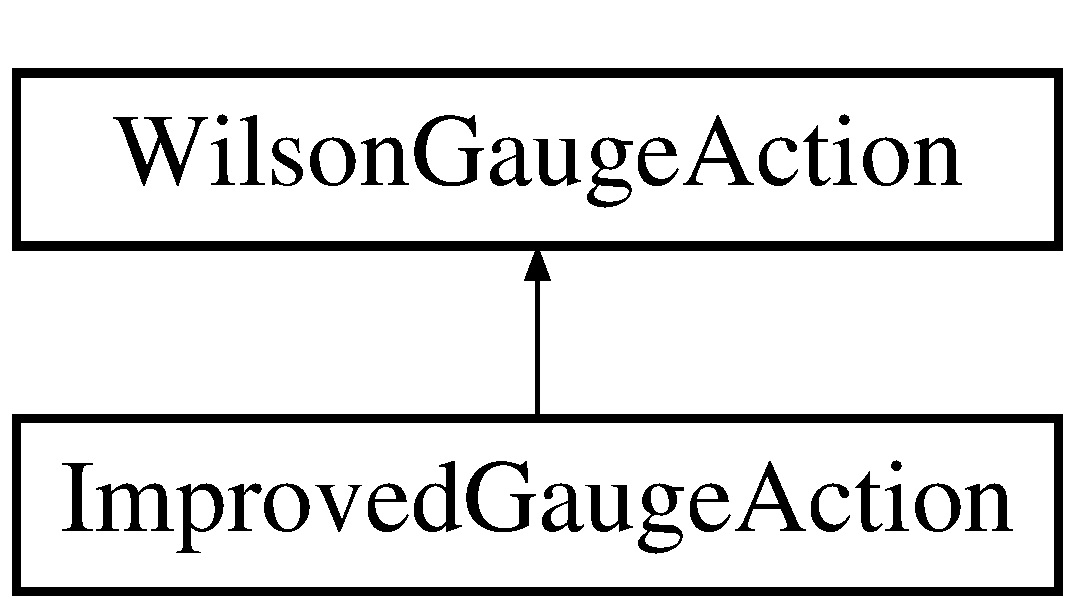
\includegraphics[height=2cm]{class_improved_gauge_action}
\end{center}
\end{figure}
\subsection*{Static Public Member Functions}
\begin{DoxyCompactItemize}
\item 
static \hyperlink{classgauge__stats}{gauge\_\-stats} \hyperlink{class_improved_gauge_action_a02e55d57665313eb939b9b6e77697680}{heatbath} (\hyperlink{classgauge__field}{gauge\_\-field} \&U, \hyperlink{classcoefficients}{coefficients} \&coeff, int n\_\-iter=1, string model=\char`\"{}MILC\char`\"{})
\end{DoxyCompactItemize}


\subsection{Detailed Description}
the $ O(a^2)$ Improved Gauge Action Example using the MILC improved action: \begin{DoxyVerb}
///    int ns=2, steps=10;
///    gauge_field U(lattice,nc);
///    coefficients gauge;
///    U.load("myfield.0000");
///    gauge["beta"]=6.0;
///    gauge["zeta"]=1.0; // MUST BE ONE
///    gauge["u_t"]=1.0;
///    gauge["u_s"]=1.0;
///    ImprovedGaugeAction::heatbath(U,gauge,steps,"MILC");
///    U.save("myfield.0001");
/// \end{DoxyVerb}
 Example using the Morningstar unisotropic improved action: \begin{DoxyVerb}
///    int ns=2, steps=10;
///    gauge_field U(lattice,nc);
///    coefficients gauge;
///    U.load("myfield.0000");
///    gauge["beta"]=6.0;
///    gauge["zeta"]=1.0; // CAN BE != ONE
///    gauge["u_t"]=1.0;
///    gauge["u_s"]=1.0;
///    ImprovedGaugeAction::heatbath(U,gauge,steps,"Morningstar");
///    U.save("myfield.0001");
/// \end{DoxyVerb}
 

\subsection{Member Function Documentation}
\hypertarget{class_improved_gauge_action_a02e55d57665313eb939b9b6e77697680}{
\index{ImprovedGaugeAction@{ImprovedGaugeAction}!heatbath@{heatbath}}
\index{heatbath@{heatbath}!ImprovedGaugeAction@{ImprovedGaugeAction}}
\subsubsection[{heatbath}]{\setlength{\rightskip}{0pt plus 5cm}static {\bf gauge\_\-stats} ImprovedGaugeAction::heatbath ({\bf gauge\_\-field} \& {\em U}, \/  {\bf coefficients} \& {\em coeff}, \/  int {\em n\_\-iter} = {\ttfamily 1}, \/  string {\em model} = {\ttfamily \char`\"{}MILC\char`\"{}})\hspace{0.3cm}{\ttfamily  \mbox{[}inline, static\mbox{]}}}}
\label{class_improved_gauge_action_a02e55d57665313eb939b9b6e77697680}


The documentation for this class was generated from the following file:\begin{DoxyCompactItemize}
\item 
/Users/mdipierro/fermiqcd/development/Libraries/\hyperlink{fermiqcd__gauge__actions_8h}{fermiqcd\_\-gauge\_\-actions.h}\end{DoxyCompactItemize}

\hypertarget{class_improved_gauge_action_s_s_e2}{
\section{ImprovedGaugeActionSSE2 Class Reference}
\label{class_improved_gauge_action_s_s_e2}\index{ImprovedGaugeActionSSE2@{ImprovedGaugeActionSSE2}}
}
the $ O(a^2)$ Improved Gauge Action for SU3 with SSE2 and double precision (UNTESTED)  


{\tt \#include $<$fermiqcd\_\-gauge\_\-actions\_\-sse2.h$>$}

Inherits \hyperlink{class_wilson_gauge_action}{WilsonGaugeAction}.

Collaboration diagram for ImprovedGaugeActionSSE2:

\subsection{Detailed Description}
the $ O(a^2)$ Improved Gauge Action for SU3 with SSE2 and double precision (UNTESTED) 

Example using the MILC improved action: 

\footnotesize\begin{verbatim}
///    int ns=2, steps=10;
///    gauge_field U(lattice,nc);
///    coefficients gauge;
///    U.load("myfield.0000");
///    gauge["beta"]=6.0;
///    gauge["zeta"]=1.0; // MUST BE ONE
///    gauge["u_t"]=1.0;
///    gauge["u_s"]=1.0;
///    ImprovedGaugeActionSSE2::heatbath(U,gauge,steps,"MILC");
///    U.save("myfield.0001");
/// \end{verbatim}
\normalsize
 Example using the Morningstar unisotropic improved action: 

\footnotesize\begin{verbatim}
///    int ns=2, steps=10;
///    gauge_field U(lattice,nc);
///    coefficients gauge;
///    U.load("myfield.0000");
///    gauge["beta"]=6.0;
///    gauge["zeta"]=1.0; // CAN BE != ONE
///    gauge["u_t"]=1.0;
///    gauge["u_s"]=1.0;
///    ImprovedGaugeActionSSE2::heatbath(U,gauge,steps,"Morningstar");
///    U.save("myfield.0001");
/// \end{verbatim}
\normalsize
 

The documentation for this class was generated from the following file:\begin{CompactItemize}
\item 
/Users/mdipierro/Desktop/SciDac/development/Libraries/\hyperlink{fermiqcd__gauge__actions__sse2_8h}{fermiqcd\_\-gauge\_\-actions\_\-sse2.h}\end{CompactItemize}

\hypertarget{class_instanton4_d}{
\section{Instanton4D Class Reference}
\label{class_instanton4_d}\index{Instanton4D@{Instanton4D}}
}


{\ttfamily \#include $<$fermiqcd\_\-instanton4d.h$>$}\subsection*{Public Member Functions}
\begin{DoxyCompactItemize}
\item 
\hyperlink{class_instanton4_d_ab23484422ea50f59e0856d51cce1cb8b}{Instanton4D} (int \hyperlink{class_instanton4_d_af8271a542264493caafca9443b0c2f38}{nc}, int \hyperlink{class_instanton4_d_a33c37212ef923556b7a1985d9e7cdd36}{sub\_\-i}, int \hyperlink{class_instanton4_d_af73c30a26883977d21e2b2e8921429cf}{sub\_\-j}, \hyperlink{mdp__global__vars_8h_a049e4c1d4e74d644878a42f9909463e4}{mdp\_\-real} \hyperlink{class_instanton4_d_a81408020baf1ea808456d691c65425e2}{charge}, \hyperlink{mdp__global__vars_8h_a049e4c1d4e74d644878a42f9909463e4}{mdp\_\-real} \hyperlink{class_instanton4_d_a69a7961ae8d9ea823cacbf8cc11bc46f}{lambda}, vector$<$ \hyperlink{mdp__global__vars_8h_a049e4c1d4e74d644878a42f9909463e4}{mdp\_\-real} $>$ \&\hyperlink{class_instanton4_d_a3d78aada54a0f8e7bafb5272cb5ca401}{p})
\item 
\hyperlink{classmdp__matrix}{mdp\_\-matrix} \hyperlink{class_instanton4_d_aa03767e0f05830b33e34b3be0f9fc447}{operator()} (\hyperlink{classmdp__site}{mdp\_\-site} \&x, int mu)
\end{DoxyCompactItemize}
\subsection*{Public Attributes}
\begin{DoxyCompactItemize}
\item 
vector$<$ \hyperlink{mdp__global__vars_8h_a049e4c1d4e74d644878a42f9909463e4}{mdp\_\-real} $>$ \hyperlink{class_instanton4_d_a3d78aada54a0f8e7bafb5272cb5ca401}{p}
\item 
int \hyperlink{class_instanton4_d_af8271a542264493caafca9443b0c2f38}{nc}
\item 
int \hyperlink{class_instanton4_d_a33c37212ef923556b7a1985d9e7cdd36}{sub\_\-i}
\item 
int \hyperlink{class_instanton4_d_af73c30a26883977d21e2b2e8921429cf}{sub\_\-j}
\item 
\hyperlink{mdp__global__vars_8h_a049e4c1d4e74d644878a42f9909463e4}{mdp\_\-real} \hyperlink{class_instanton4_d_a81408020baf1ea808456d691c65425e2}{charge}
\item 
\hyperlink{mdp__global__vars_8h_a049e4c1d4e74d644878a42f9909463e4}{mdp\_\-real} \hyperlink{class_instanton4_d_a69a7961ae8d9ea823cacbf8cc11bc46f}{lambda}
\item 
\hyperlink{classmdp__matrix}{mdp\_\-matrix} \hyperlink{class_instanton4_d_ae318efcecc72b47fb7b43bcf0222697f}{eta} \mbox{[}4\mbox{]}\mbox{[}4\mbox{]}
\end{DoxyCompactItemize}


\subsection{Constructor \& Destructor Documentation}
\hypertarget{class_instanton4_d_ab23484422ea50f59e0856d51cce1cb8b}{
\index{Instanton4D@{Instanton4D}!Instanton4D@{Instanton4D}}
\index{Instanton4D@{Instanton4D}!Instanton4D@{Instanton4D}}
\subsubsection[{Instanton4D}]{\setlength{\rightskip}{0pt plus 5cm}Instanton4D::Instanton4D (int {\em nc}, \/  int {\em sub\_\-i}, \/  int {\em sub\_\-j}, \/  {\bf mdp\_\-real} {\em charge}, \/  {\bf mdp\_\-real} {\em lambda}, \/  vector$<$ {\bf mdp\_\-real} $>$ \& {\em p})\hspace{0.3cm}{\ttfamily  \mbox{[}inline\mbox{]}}}}
\label{class_instanton4_d_ab23484422ea50f59e0856d51cce1cb8b}


\subsection{Member Function Documentation}
\hypertarget{class_instanton4_d_aa03767e0f05830b33e34b3be0f9fc447}{
\index{Instanton4D@{Instanton4D}!operator()@{operator()}}
\index{operator()@{operator()}!Instanton4D@{Instanton4D}}
\subsubsection[{operator()}]{\setlength{\rightskip}{0pt plus 5cm}{\bf mdp\_\-matrix} Instanton4D::operator() ({\bf mdp\_\-site} \& {\em x}, \/  int {\em mu})\hspace{0.3cm}{\ttfamily  \mbox{[}inline\mbox{]}}}}
\label{class_instanton4_d_aa03767e0f05830b33e34b3be0f9fc447}


\subsection{Member Data Documentation}
\hypertarget{class_instanton4_d_a81408020baf1ea808456d691c65425e2}{
\index{Instanton4D@{Instanton4D}!charge@{charge}}
\index{charge@{charge}!Instanton4D@{Instanton4D}}
\subsubsection[{charge}]{\setlength{\rightskip}{0pt plus 5cm}{\bf mdp\_\-real} {\bf Instanton4D::charge}}}
\label{class_instanton4_d_a81408020baf1ea808456d691c65425e2}
\hypertarget{class_instanton4_d_ae318efcecc72b47fb7b43bcf0222697f}{
\index{Instanton4D@{Instanton4D}!eta@{eta}}
\index{eta@{eta}!Instanton4D@{Instanton4D}}
\subsubsection[{eta}]{\setlength{\rightskip}{0pt plus 5cm}{\bf mdp\_\-matrix} {\bf Instanton4D::eta}\mbox{[}4\mbox{]}\mbox{[}4\mbox{]}}}
\label{class_instanton4_d_ae318efcecc72b47fb7b43bcf0222697f}
\hypertarget{class_instanton4_d_a69a7961ae8d9ea823cacbf8cc11bc46f}{
\index{Instanton4D@{Instanton4D}!lambda@{lambda}}
\index{lambda@{lambda}!Instanton4D@{Instanton4D}}
\subsubsection[{lambda}]{\setlength{\rightskip}{0pt plus 5cm}{\bf mdp\_\-real} {\bf Instanton4D::lambda}}}
\label{class_instanton4_d_a69a7961ae8d9ea823cacbf8cc11bc46f}
\hypertarget{class_instanton4_d_af8271a542264493caafca9443b0c2f38}{
\index{Instanton4D@{Instanton4D}!nc@{nc}}
\index{nc@{nc}!Instanton4D@{Instanton4D}}
\subsubsection[{nc}]{\setlength{\rightskip}{0pt plus 5cm}int {\bf Instanton4D::nc}}}
\label{class_instanton4_d_af8271a542264493caafca9443b0c2f38}
\hypertarget{class_instanton4_d_a3d78aada54a0f8e7bafb5272cb5ca401}{
\index{Instanton4D@{Instanton4D}!p@{p}}
\index{p@{p}!Instanton4D@{Instanton4D}}
\subsubsection[{p}]{\setlength{\rightskip}{0pt plus 5cm}vector$<${\bf mdp\_\-real}$>$ {\bf Instanton4D::p}}}
\label{class_instanton4_d_a3d78aada54a0f8e7bafb5272cb5ca401}
\hypertarget{class_instanton4_d_a33c37212ef923556b7a1985d9e7cdd36}{
\index{Instanton4D@{Instanton4D}!sub\_\-i@{sub\_\-i}}
\index{sub\_\-i@{sub\_\-i}!Instanton4D@{Instanton4D}}
\subsubsection[{sub\_\-i}]{\setlength{\rightskip}{0pt plus 5cm}int {\bf Instanton4D::sub\_\-i}}}
\label{class_instanton4_d_a33c37212ef923556b7a1985d9e7cdd36}
\hypertarget{class_instanton4_d_af73c30a26883977d21e2b2e8921429cf}{
\index{Instanton4D@{Instanton4D}!sub\_\-j@{sub\_\-j}}
\index{sub\_\-j@{sub\_\-j}!Instanton4D@{Instanton4D}}
\subsubsection[{sub\_\-j}]{\setlength{\rightskip}{0pt plus 5cm}int {\bf Instanton4D::sub\_\-j}}}
\label{class_instanton4_d_af73c30a26883977d21e2b2e8921429cf}


The documentation for this class was generated from the following file:\begin{DoxyCompactItemize}
\item 
/Users/mdipierro/fermiqcd/development/Libraries/\hyperlink{fermiqcd__instanton4d_8h}{fermiqcd\_\-instanton4d.h}\end{DoxyCompactItemize}

\hypertarget{classinversion__stats}{
\section{inversion\_\-stats Class Reference}
\label{classinversion__stats}\index{inversion\_\-stats@{inversion\_\-stats}}
}


structure for inverstion stats  


{\ttfamily \#include $<$fermiqcd\_\-minres\_\-inverter.h$>$}\subsection*{Public Attributes}
\begin{DoxyCompactItemize}
\item 
\hyperlink{mdp__global__vars_8h_a049e4c1d4e74d644878a42f9909463e4}{mdp\_\-real} \hyperlink{classinversion__stats_aa3e398f27da37c39f825b407829e8c15}{target\_\-absolute\_\-precision}
\item 
\hyperlink{mdp__global__vars_8h_a049e4c1d4e74d644878a42f9909463e4}{mdp\_\-real} \hyperlink{classinversion__stats_a57f0e5274f6057d41a9e386d2d3d213e}{target\_\-relative\_\-precision}
\item 
int \hyperlink{classinversion__stats_ad11085b60e91bb439a125457fc16c69a}{max\_\-steps}
\item 
\hyperlink{mdp__global__vars_8h_a049e4c1d4e74d644878a42f9909463e4}{mdp\_\-real} \hyperlink{classinversion__stats_a6463ea546805e548502803d09c7b74f0}{residue}
\item 
\hyperlink{mdp__global__vars_8h_a049e4c1d4e74d644878a42f9909463e4}{mdp\_\-real} \hyperlink{classinversion__stats_aba965f93a417bb48f9d01933cbacc46e}{absolute\_\-precision}
\item 
\hyperlink{mdp__global__vars_8h_a049e4c1d4e74d644878a42f9909463e4}{mdp\_\-real} \hyperlink{classinversion__stats_a3bbfed38efd2f5669aaee413676f0d4a}{relative\_\-precision}
\item 
int \hyperlink{classinversion__stats_aabd17c3bb1476dc06843ed171ea53253}{steps}
\item 
int \hyperlink{classinversion__stats_a392e51a8f0ced3098ce309018dfa932c}{mul\_\-Q\_\-steps}
\item 
\hyperlink{mdp__global__vars_8h_a049e4c1d4e74d644878a42f9909463e4}{mdp\_\-real} \hyperlink{classinversion__stats_a648a0c2aae15866e7331d0cd4d0736ff}{time}
\end{DoxyCompactItemize}


\subsection{Detailed Description}
structure for inverstion stats Returned by the inverters 

\subsection{Member Data Documentation}
\hypertarget{classinversion__stats_aba965f93a417bb48f9d01933cbacc46e}{
\index{inversion\_\-stats@{inversion\_\-stats}!absolute\_\-precision@{absolute\_\-precision}}
\index{absolute\_\-precision@{absolute\_\-precision}!inversion_stats@{inversion\_\-stats}}
\subsubsection[{absolute\_\-precision}]{\setlength{\rightskip}{0pt plus 5cm}{\bf mdp\_\-real} {\bf inversion\_\-stats::absolute\_\-precision}}}
\label{classinversion__stats_aba965f93a417bb48f9d01933cbacc46e}
\hypertarget{classinversion__stats_ad11085b60e91bb439a125457fc16c69a}{
\index{inversion\_\-stats@{inversion\_\-stats}!max\_\-steps@{max\_\-steps}}
\index{max\_\-steps@{max\_\-steps}!inversion_stats@{inversion\_\-stats}}
\subsubsection[{max\_\-steps}]{\setlength{\rightskip}{0pt plus 5cm}int {\bf inversion\_\-stats::max\_\-steps}}}
\label{classinversion__stats_ad11085b60e91bb439a125457fc16c69a}
\hypertarget{classinversion__stats_a392e51a8f0ced3098ce309018dfa932c}{
\index{inversion\_\-stats@{inversion\_\-stats}!mul\_\-Q\_\-steps@{mul\_\-Q\_\-steps}}
\index{mul\_\-Q\_\-steps@{mul\_\-Q\_\-steps}!inversion_stats@{inversion\_\-stats}}
\subsubsection[{mul\_\-Q\_\-steps}]{\setlength{\rightskip}{0pt plus 5cm}int {\bf inversion\_\-stats::mul\_\-Q\_\-steps}}}
\label{classinversion__stats_a392e51a8f0ced3098ce309018dfa932c}
\hypertarget{classinversion__stats_a3bbfed38efd2f5669aaee413676f0d4a}{
\index{inversion\_\-stats@{inversion\_\-stats}!relative\_\-precision@{relative\_\-precision}}
\index{relative\_\-precision@{relative\_\-precision}!inversion_stats@{inversion\_\-stats}}
\subsubsection[{relative\_\-precision}]{\setlength{\rightskip}{0pt plus 5cm}{\bf mdp\_\-real} {\bf inversion\_\-stats::relative\_\-precision}}}
\label{classinversion__stats_a3bbfed38efd2f5669aaee413676f0d4a}
\hypertarget{classinversion__stats_a6463ea546805e548502803d09c7b74f0}{
\index{inversion\_\-stats@{inversion\_\-stats}!residue@{residue}}
\index{residue@{residue}!inversion_stats@{inversion\_\-stats}}
\subsubsection[{residue}]{\setlength{\rightskip}{0pt plus 5cm}{\bf mdp\_\-real} {\bf inversion\_\-stats::residue}}}
\label{classinversion__stats_a6463ea546805e548502803d09c7b74f0}
\hypertarget{classinversion__stats_aabd17c3bb1476dc06843ed171ea53253}{
\index{inversion\_\-stats@{inversion\_\-stats}!steps@{steps}}
\index{steps@{steps}!inversion_stats@{inversion\_\-stats}}
\subsubsection[{steps}]{\setlength{\rightskip}{0pt plus 5cm}int {\bf inversion\_\-stats::steps}}}
\label{classinversion__stats_aabd17c3bb1476dc06843ed171ea53253}
\hypertarget{classinversion__stats_aa3e398f27da37c39f825b407829e8c15}{
\index{inversion\_\-stats@{inversion\_\-stats}!target\_\-absolute\_\-precision@{target\_\-absolute\_\-precision}}
\index{target\_\-absolute\_\-precision@{target\_\-absolute\_\-precision}!inversion_stats@{inversion\_\-stats}}
\subsubsection[{target\_\-absolute\_\-precision}]{\setlength{\rightskip}{0pt plus 5cm}{\bf mdp\_\-real} {\bf inversion\_\-stats::target\_\-absolute\_\-precision}}}
\label{classinversion__stats_aa3e398f27da37c39f825b407829e8c15}
\hypertarget{classinversion__stats_a57f0e5274f6057d41a9e386d2d3d213e}{
\index{inversion\_\-stats@{inversion\_\-stats}!target\_\-relative\_\-precision@{target\_\-relative\_\-precision}}
\index{target\_\-relative\_\-precision@{target\_\-relative\_\-precision}!inversion_stats@{inversion\_\-stats}}
\subsubsection[{target\_\-relative\_\-precision}]{\setlength{\rightskip}{0pt plus 5cm}{\bf mdp\_\-real} {\bf inversion\_\-stats::target\_\-relative\_\-precision}}}
\label{classinversion__stats_a57f0e5274f6057d41a9e386d2d3d213e}
\hypertarget{classinversion__stats_a648a0c2aae15866e7331d0cd4d0736ff}{
\index{inversion\_\-stats@{inversion\_\-stats}!time@{time}}
\index{time@{time}!inversion_stats@{inversion\_\-stats}}
\subsubsection[{time}]{\setlength{\rightskip}{0pt plus 5cm}{\bf mdp\_\-real} {\bf inversion\_\-stats::time}}}
\label{classinversion__stats_a648a0c2aae15866e7331d0cd4d0736ff}


The documentation for this class was generated from the following file:\begin{DoxyCompactItemize}
\item 
/Users/mdipierro/fermiqcd/development/Libraries/\hyperlink{fermiqcd__minres__inverter_8h}{fermiqcd\_\-minres\_\-inverter.h}\end{DoxyCompactItemize}

\hypertarget{class_lanczos}{
\section{Lanczos$<$ fieldT $>$ Class Template Reference}
\label{class_lanczos}\index{Lanczos@{Lanczos}}
}


\hyperlink{class_lanczos}{Lanczos} algorithms.  


{\ttfamily \#include $<$fermiqcd\_\-lanczos.h$>$}\subsection*{Static Public Member Functions}
\begin{DoxyCompactItemize}
\item 
static \hyperlink{classmdp__complex}{mdp\_\-complex} \hyperlink{class_lanczos_a955801bdbd7665b16d35b60de725636e}{step} (fieldT \&psi, \hyperlink{classgauge__field}{gauge\_\-field} \&U, \hyperlink{classcoefficients}{coefficients} \&coeff, bool force=false, bool output\_\-check=false)
\end{DoxyCompactItemize}


\subsection{Detailed Description}
\subsubsection*{template$<$class fieldT$>$ class Lanczos$<$ fieldT $>$}

\hyperlink{class_lanczos}{Lanczos} algorithms. Example: \begin{DoxyVerb}
/// mdp_gauge U(lattice,nc);
/// fermi_field psi(lattice,nc);
/// coefficients coeff;
/// coeff["kappa"]=1.12;
/// for(int k=0; k<100; k++)
///    mdp << Lanczos::step(psi,U,coeff) << endl;
/// \end{DoxyVerb}
 return mdp\_\-complex(alpha,eta) 

\subsection{Member Function Documentation}
\hypertarget{class_lanczos_a955801bdbd7665b16d35b60de725636e}{
\index{Lanczos@{Lanczos}!step@{step}}
\index{step@{step}!Lanczos@{Lanczos}}
\subsubsection[{step}]{\setlength{\rightskip}{0pt plus 5cm}template$<$class fieldT $>$ static {\bf mdp\_\-complex} {\bf Lanczos}$<$ fieldT $>$::step (fieldT \& {\em psi}, \/  {\bf gauge\_\-field} \& {\em U}, \/  {\bf coefficients} \& {\em coeff}, \/  bool {\em force} = {\ttfamily false}, \/  bool {\em output\_\-check} = {\ttfamily false})\hspace{0.3cm}{\ttfamily  \mbox{[}inline, static\mbox{]}}}}
\label{class_lanczos_a955801bdbd7665b16d35b60de725636e}


The documentation for this class was generated from the following file:\begin{DoxyCompactItemize}
\item 
/Users/mdipierro/fermiqcd/development/Libraries/\hyperlink{fermiqcd__lanczos_8h}{fermiqcd\_\-lanczos.h}\end{DoxyCompactItemize}

\hypertarget{classmdp__array}{
\section{mdp\_\-array$<$ T, nc\_\- $>$ Class Template Reference}
\label{classmdp__array}\index{mdp\_\-array@{mdp\_\-array}}
}


generic container for multidimensional arrays  


{\ttfamily \#include $<$mdp\_\-array.h$>$}\subsection*{Public Member Functions}
\begin{DoxyCompactItemize}
\item 
const int \& \hyperlink{classmdp__array_a20f4c81199739f0465af62c811cd60b7}{ndim} () const 
\item 
T $\ast$ \hyperlink{classmdp__array_a9b5419e65691954be0a3b6598a47366a}{address} ()
\item 
\hyperlink{mdp__global__vars_8h_a91ad9478d81a7aaf2593e8d9c3d06a14}{uint} $\ast$ \hyperlink{classmdp__array_aee0c0b97d3f8bb9d3f8ecedb77d14e6d}{size\_\-address} ()
\item 
T \& \hyperlink{classmdp__array_acc0201400e730c01bd131696ff206aa6}{operator\mbox{[}$\,$\mbox{]}} (const \hyperlink{mdp__global__vars_8h_a91ad9478d81a7aaf2593e8d9c3d06a14}{uint} i)
\item 
const T \& \hyperlink{classmdp__array_a7c6f82ec888e82f3743529ac25d42627}{operator\mbox{[}$\,$\mbox{]}} (const \hyperlink{mdp__global__vars_8h_a91ad9478d81a7aaf2593e8d9c3d06a14}{uint} i) const 
\item 
\hyperlink{mdp__global__vars_8h_a91ad9478d81a7aaf2593e8d9c3d06a14}{uint} \hyperlink{classmdp__array_a4856c3ff5dbeeb3479a531e0c505559f}{length} (const \hyperlink{mdp__global__vars_8h_a91ad9478d81a7aaf2593e8d9c3d06a14}{uint} i) const 
\item 
\hyperlink{mdp__global__vars_8h_a91ad9478d81a7aaf2593e8d9c3d06a14}{uint} \hyperlink{classmdp__array_a5e8cd60cd274b3a0e9835b66c6d430e6}{length} () const 
\item 
\hyperlink{mdp__global__vars_8h_a91ad9478d81a7aaf2593e8d9c3d06a14}{uint} \hyperlink{classmdp__array_adf2fd9006ccac4f6b1365d4018f3e513}{size} (\hyperlink{mdp__global__vars_8h_a91ad9478d81a7aaf2593e8d9c3d06a14}{uint} i) const 
\item 
\hyperlink{mdp__global__vars_8h_a91ad9478d81a7aaf2593e8d9c3d06a14}{uint} \hyperlink{classmdp__array_a236c3497ad1e959070836746302448e8}{size} () const 
\item 
void \hyperlink{classmdp__array_a6a3d01021b01c27ea0a0cf43dd442ad5}{dimension} (const \hyperlink{mdp__global__vars_8h_a91ad9478d81a7aaf2593e8d9c3d06a14}{uint} $\ast$p)
\item 
void \hyperlink{classmdp__array_a816b392dd8ab232c18818e6f186127aa}{dimension} (const \hyperlink{mdp__global__vars_8h_a91ad9478d81a7aaf2593e8d9c3d06a14}{uint} c0\_\-=1, const \hyperlink{mdp__global__vars_8h_a91ad9478d81a7aaf2593e8d9c3d06a14}{uint} c1\_\-=1, const \hyperlink{mdp__global__vars_8h_a91ad9478d81a7aaf2593e8d9c3d06a14}{uint} c2\_\-=1, const \hyperlink{mdp__global__vars_8h_a91ad9478d81a7aaf2593e8d9c3d06a14}{uint} c3\_\-=1, const \hyperlink{mdp__global__vars_8h_a91ad9478d81a7aaf2593e8d9c3d06a14}{uint} c4\_\-=1)
\item 
\hyperlink{classmdp__array_a231c442576ed1a88e333fb88bcedef41}{mdp\_\-array} (const \hyperlink{mdp__global__vars_8h_a91ad9478d81a7aaf2593e8d9c3d06a14}{uint} c0\_\-=1, const \hyperlink{mdp__global__vars_8h_a91ad9478d81a7aaf2593e8d9c3d06a14}{uint} c1\_\-=1, const \hyperlink{mdp__global__vars_8h_a91ad9478d81a7aaf2593e8d9c3d06a14}{uint} c2\_\-=1, const \hyperlink{mdp__global__vars_8h_a91ad9478d81a7aaf2593e8d9c3d06a14}{uint} c3\_\-=1, const \hyperlink{mdp__global__vars_8h_a91ad9478d81a7aaf2593e8d9c3d06a14}{uint} c4\_\-=1)
\item 
\hyperlink{classmdp__array_a7bdd0c532c8517bf46bceab7c48f3186}{mdp\_\-array} (const \hyperlink{mdp__global__vars_8h_a91ad9478d81a7aaf2593e8d9c3d06a14}{uint} $\ast$p)
\item 
\hyperlink{classmdp__array_abf3b0ca804544eac3be7d8e499eeb089}{mdp\_\-array} (const T $\ast$m0, const \hyperlink{mdp__global__vars_8h_a91ad9478d81a7aaf2593e8d9c3d06a14}{uint} c0\_\-=1, const \hyperlink{mdp__global__vars_8h_a91ad9478d81a7aaf2593e8d9c3d06a14}{uint} c1\_\-=1, const \hyperlink{mdp__global__vars_8h_a91ad9478d81a7aaf2593e8d9c3d06a14}{uint} c2\_\-=1, const \hyperlink{mdp__global__vars_8h_a91ad9478d81a7aaf2593e8d9c3d06a14}{uint} c3\_\-=1, const \hyperlink{mdp__global__vars_8h_a91ad9478d81a7aaf2593e8d9c3d06a14}{uint} c4\_\-=1)
\item 
\hyperlink{classmdp__array_a1932c8ea14f2fc8cb7343f9834154521}{mdp\_\-array} (const T $\ast$m0, const \hyperlink{mdp__global__vars_8h_a91ad9478d81a7aaf2593e8d9c3d06a14}{uint} $\ast$p)
\item 
\hyperlink{classmdp__array_af266114d51b7b0e038cb555ba02d83d4}{mdp\_\-array} (const \hyperlink{classmdp__array}{mdp\_\-array} \&a)
\item 
virtual \hyperlink{classmdp__array_a962dc25e9c53d9f6e215b0ef952fc96b}{$\sim$mdp\_\-array} ()
\item 
void \hyperlink{classmdp__array_a8f439abc20da235f12cd5d0ab4d7b56b}{operator=} (const \hyperlink{classmdp__array}{mdp\_\-array} \&a)
\item 
T \& \hyperlink{classmdp__array_a9e3a7e699387fb78562fb8d9c9ebea57}{operator()} (const \hyperlink{mdp__global__vars_8h_a91ad9478d81a7aaf2593e8d9c3d06a14}{uint} i0, const \hyperlink{mdp__global__vars_8h_a91ad9478d81a7aaf2593e8d9c3d06a14}{uint} i1=0, const \hyperlink{mdp__global__vars_8h_a91ad9478d81a7aaf2593e8d9c3d06a14}{uint} i2=0, const \hyperlink{mdp__global__vars_8h_a91ad9478d81a7aaf2593e8d9c3d06a14}{uint} i3=0, const \hyperlink{mdp__global__vars_8h_a91ad9478d81a7aaf2593e8d9c3d06a14}{uint} i4=0)
\item 
const T \& \hyperlink{classmdp__array_a9ddceeb1b33b80495ef45afb812c0012}{operator()} (const \hyperlink{mdp__global__vars_8h_a91ad9478d81a7aaf2593e8d9c3d06a14}{uint} i0, const \hyperlink{mdp__global__vars_8h_a91ad9478d81a7aaf2593e8d9c3d06a14}{uint} i1=0, const \hyperlink{mdp__global__vars_8h_a91ad9478d81a7aaf2593e8d9c3d06a14}{uint} i2=0, const \hyperlink{mdp__global__vars_8h_a91ad9478d81a7aaf2593e8d9c3d06a14}{uint} i3=0, const \hyperlink{mdp__global__vars_8h_a91ad9478d81a7aaf2593e8d9c3d06a14}{uint} i4=0) const 
\end{DoxyCompactItemize}
\subsection*{Friends}
\begin{DoxyCompactItemize}
\item 
void \hyperlink{classmdp__array_a7c12113e8b61f3906ff4d15a6cc10fe2}{prepare} (const \hyperlink{classmdp__array}{mdp\_\-array} \&a)
\item 
\hyperlink{classmdp__array}{mdp\_\-array} \hyperlink{classmdp__array_a0456c0c6d5e305cc0799ceb7b8639539}{operator+} (const \hyperlink{classmdp__array}{mdp\_\-array} \&a, const \hyperlink{classmdp__array}{mdp\_\-array} \&b)
\item 
\hyperlink{classmdp__array}{mdp\_\-array} \hyperlink{classmdp__array_a97528690c485585f95cfad74e934e621}{operator-\/} (const \hyperlink{classmdp__array}{mdp\_\-array} \&a, const \hyperlink{classmdp__array}{mdp\_\-array} \&b)
\item 
{\footnotesize template$<$class T2 $>$ }\\\hyperlink{classmdp__array}{mdp\_\-array} \hyperlink{classmdp__array_a153656d696c7d05f5e61deb324e93132}{operator$\ast$} (T2 x, const \hyperlink{classmdp__array}{mdp\_\-array} \&a)
\item 
\hyperlink{classmdp__array}{mdp\_\-array} \hyperlink{classmdp__array_a720a0f3e6c74893b0bb90ddb85e2c7cf}{applytoall} (const \hyperlink{classmdp__array}{mdp\_\-array} \&a, T($\ast$fptr)(T, void $\ast$), void $\ast$x=0)
\item 
\hyperlink{classmdp__array}{mdp\_\-array} \hyperlink{classmdp__array_af47ee2aa085a0ca303f6eb960be0b257}{applytoall} (const \hyperlink{classmdp__array}{mdp\_\-array} \&a, const \hyperlink{classmdp__array}{mdp\_\-array} \&b, T($\ast$fptr)(T, T, void $\ast$), void $\ast$x=0)
\item 
ostream \& \hyperlink{classmdp__array_a5b84c698961f9276308a57923daf4458}{operator$<$$<$} (ostream \&os, const \hyperlink{classmdp__array}{mdp\_\-array} \&a)
\end{DoxyCompactItemize}


\subsection{Detailed Description}
\subsubsection*{template$<$class T, uint nc\_\-$>$ class mdp\_\-array$<$ T, nc\_\- $>$}

generic container for multidimensional arrays Example: \begin{DoxyVerb}
///    mdp_array<float,3> a(5,5,5);
///    a(0,0,0)=3.15;
/// \end{DoxyVerb}
 

\subsection{Constructor \& Destructor Documentation}
\hypertarget{classmdp__array_a231c442576ed1a88e333fb88bcedef41}{
\index{mdp\_\-array@{mdp\_\-array}!mdp\_\-array@{mdp\_\-array}}
\index{mdp\_\-array@{mdp\_\-array}!mdp_array@{mdp\_\-array}}
\subsubsection[{mdp\_\-array}]{\setlength{\rightskip}{0pt plus 5cm}template$<$class T, uint nc\_\-$>$ {\bf mdp\_\-array}$<$ T, nc\_\- $>$::{\bf mdp\_\-array} (const {\bf uint} {\em c0\_\-} = {\ttfamily 1}, \/  const {\bf uint} {\em c1\_\-} = {\ttfamily 1}, \/  const {\bf uint} {\em c2\_\-} = {\ttfamily 1}, \/  const {\bf uint} {\em c3\_\-} = {\ttfamily 1}, \/  const {\bf uint} {\em c4\_\-} = {\ttfamily 1})\hspace{0.3cm}{\ttfamily  \mbox{[}inline\mbox{]}}}}
\label{classmdp__array_a231c442576ed1a88e333fb88bcedef41}
\hypertarget{classmdp__array_a7bdd0c532c8517bf46bceab7c48f3186}{
\index{mdp\_\-array@{mdp\_\-array}!mdp\_\-array@{mdp\_\-array}}
\index{mdp\_\-array@{mdp\_\-array}!mdp_array@{mdp\_\-array}}
\subsubsection[{mdp\_\-array}]{\setlength{\rightskip}{0pt plus 5cm}template$<$class T, uint nc\_\-$>$ {\bf mdp\_\-array}$<$ T, nc\_\- $>$::{\bf mdp\_\-array} (const {\bf uint} $\ast$ {\em p})\hspace{0.3cm}{\ttfamily  \mbox{[}inline\mbox{]}}}}
\label{classmdp__array_a7bdd0c532c8517bf46bceab7c48f3186}
\hypertarget{classmdp__array_abf3b0ca804544eac3be7d8e499eeb089}{
\index{mdp\_\-array@{mdp\_\-array}!mdp\_\-array@{mdp\_\-array}}
\index{mdp\_\-array@{mdp\_\-array}!mdp_array@{mdp\_\-array}}
\subsubsection[{mdp\_\-array}]{\setlength{\rightskip}{0pt plus 5cm}template$<$class T, uint nc\_\-$>$ {\bf mdp\_\-array}$<$ T, nc\_\- $>$::{\bf mdp\_\-array} (const T $\ast$ {\em m0}, \/  const {\bf uint} {\em c0\_\-} = {\ttfamily 1}, \/  const {\bf uint} {\em c1\_\-} = {\ttfamily 1}, \/  const {\bf uint} {\em c2\_\-} = {\ttfamily 1}, \/  const {\bf uint} {\em c3\_\-} = {\ttfamily 1}, \/  const {\bf uint} {\em c4\_\-} = {\ttfamily 1})\hspace{0.3cm}{\ttfamily  \mbox{[}inline\mbox{]}}}}
\label{classmdp__array_abf3b0ca804544eac3be7d8e499eeb089}
\hypertarget{classmdp__array_a1932c8ea14f2fc8cb7343f9834154521}{
\index{mdp\_\-array@{mdp\_\-array}!mdp\_\-array@{mdp\_\-array}}
\index{mdp\_\-array@{mdp\_\-array}!mdp_array@{mdp\_\-array}}
\subsubsection[{mdp\_\-array}]{\setlength{\rightskip}{0pt plus 5cm}template$<$class T, uint nc\_\-$>$ {\bf mdp\_\-array}$<$ T, nc\_\- $>$::{\bf mdp\_\-array} (const T $\ast$ {\em m0}, \/  const {\bf uint} $\ast$ {\em p})\hspace{0.3cm}{\ttfamily  \mbox{[}inline\mbox{]}}}}
\label{classmdp__array_a1932c8ea14f2fc8cb7343f9834154521}
\hypertarget{classmdp__array_af266114d51b7b0e038cb555ba02d83d4}{
\index{mdp\_\-array@{mdp\_\-array}!mdp\_\-array@{mdp\_\-array}}
\index{mdp\_\-array@{mdp\_\-array}!mdp_array@{mdp\_\-array}}
\subsubsection[{mdp\_\-array}]{\setlength{\rightskip}{0pt plus 5cm}template$<$class T, uint nc\_\-$>$ {\bf mdp\_\-array}$<$ T, nc\_\- $>$::{\bf mdp\_\-array} (const {\bf mdp\_\-array}$<$ T, nc\_\- $>$ \& {\em a})\hspace{0.3cm}{\ttfamily  \mbox{[}inline\mbox{]}}}}
\label{classmdp__array_af266114d51b7b0e038cb555ba02d83d4}
\hypertarget{classmdp__array_a962dc25e9c53d9f6e215b0ef952fc96b}{
\index{mdp\_\-array@{mdp\_\-array}!$\sim$mdp\_\-array@{$\sim$mdp\_\-array}}
\index{$\sim$mdp\_\-array@{$\sim$mdp\_\-array}!mdp_array@{mdp\_\-array}}
\subsubsection[{$\sim$mdp\_\-array}]{\setlength{\rightskip}{0pt plus 5cm}template$<$class T, uint nc\_\-$>$ virtual {\bf mdp\_\-array}$<$ T, nc\_\- $>$::$\sim${\bf mdp\_\-array} ()\hspace{0.3cm}{\ttfamily  \mbox{[}inline, virtual\mbox{]}}}}
\label{classmdp__array_a962dc25e9c53d9f6e215b0ef952fc96b}


\subsection{Member Function Documentation}
\hypertarget{classmdp__array_a9b5419e65691954be0a3b6598a47366a}{
\index{mdp\_\-array@{mdp\_\-array}!address@{address}}
\index{address@{address}!mdp_array@{mdp\_\-array}}
\subsubsection[{address}]{\setlength{\rightskip}{0pt plus 5cm}template$<$class T, uint nc\_\-$>$ T$\ast$ {\bf mdp\_\-array}$<$ T, nc\_\- $>$::address ()\hspace{0.3cm}{\ttfamily  \mbox{[}inline\mbox{]}}}}
\label{classmdp__array_a9b5419e65691954be0a3b6598a47366a}
\hypertarget{classmdp__array_a816b392dd8ab232c18818e6f186127aa}{
\index{mdp\_\-array@{mdp\_\-array}!dimension@{dimension}}
\index{dimension@{dimension}!mdp_array@{mdp\_\-array}}
\subsubsection[{dimension}]{\setlength{\rightskip}{0pt plus 5cm}template$<$class T, uint nc\_\-$>$ void {\bf mdp\_\-array}$<$ T, nc\_\- $>$::dimension (const {\bf uint} {\em c0\_\-} = {\ttfamily 1}, \/  const {\bf uint} {\em c1\_\-} = {\ttfamily 1}, \/  const {\bf uint} {\em c2\_\-} = {\ttfamily 1}, \/  const {\bf uint} {\em c3\_\-} = {\ttfamily 1}, \/  const {\bf uint} {\em c4\_\-} = {\ttfamily 1})\hspace{0.3cm}{\ttfamily  \mbox{[}inline\mbox{]}}}}
\label{classmdp__array_a816b392dd8ab232c18818e6f186127aa}
\hypertarget{classmdp__array_a6a3d01021b01c27ea0a0cf43dd442ad5}{
\index{mdp\_\-array@{mdp\_\-array}!dimension@{dimension}}
\index{dimension@{dimension}!mdp_array@{mdp\_\-array}}
\subsubsection[{dimension}]{\setlength{\rightskip}{0pt plus 5cm}template$<$class T, uint nc\_\-$>$ void {\bf mdp\_\-array}$<$ T, nc\_\- $>$::dimension (const {\bf uint} $\ast$ {\em p})\hspace{0.3cm}{\ttfamily  \mbox{[}inline\mbox{]}}}}
\label{classmdp__array_a6a3d01021b01c27ea0a0cf43dd442ad5}
\hypertarget{classmdp__array_a5e8cd60cd274b3a0e9835b66c6d430e6}{
\index{mdp\_\-array@{mdp\_\-array}!length@{length}}
\index{length@{length}!mdp_array@{mdp\_\-array}}
\subsubsection[{length}]{\setlength{\rightskip}{0pt plus 5cm}template$<$class T, uint nc\_\-$>$ {\bf uint} {\bf mdp\_\-array}$<$ T, nc\_\- $>$::length () const\hspace{0.3cm}{\ttfamily  \mbox{[}inline\mbox{]}}}}
\label{classmdp__array_a5e8cd60cd274b3a0e9835b66c6d430e6}
\hypertarget{classmdp__array_a4856c3ff5dbeeb3479a531e0c505559f}{
\index{mdp\_\-array@{mdp\_\-array}!length@{length}}
\index{length@{length}!mdp_array@{mdp\_\-array}}
\subsubsection[{length}]{\setlength{\rightskip}{0pt plus 5cm}template$<$class T, uint nc\_\-$>$ {\bf uint} {\bf mdp\_\-array}$<$ T, nc\_\- $>$::length (const {\bf uint} {\em i}) const\hspace{0.3cm}{\ttfamily  \mbox{[}inline\mbox{]}}}}
\label{classmdp__array_a4856c3ff5dbeeb3479a531e0c505559f}
\hypertarget{classmdp__array_a20f4c81199739f0465af62c811cd60b7}{
\index{mdp\_\-array@{mdp\_\-array}!ndim@{ndim}}
\index{ndim@{ndim}!mdp_array@{mdp\_\-array}}
\subsubsection[{ndim}]{\setlength{\rightskip}{0pt plus 5cm}template$<$class T, uint nc\_\-$>$ const int\& {\bf mdp\_\-array}$<$ T, nc\_\- $>$::ndim () const\hspace{0.3cm}{\ttfamily  \mbox{[}inline\mbox{]}}}}
\label{classmdp__array_a20f4c81199739f0465af62c811cd60b7}
\hypertarget{classmdp__array_a9ddceeb1b33b80495ef45afb812c0012}{
\index{mdp\_\-array@{mdp\_\-array}!operator()@{operator()}}
\index{operator()@{operator()}!mdp_array@{mdp\_\-array}}
\subsubsection[{operator()}]{\setlength{\rightskip}{0pt plus 5cm}template$<$class T, uint nc\_\-$>$ const T\& {\bf mdp\_\-array}$<$ T, nc\_\- $>$::operator() (const {\bf uint} {\em i0}, \/  const {\bf uint} {\em i1} = {\ttfamily 0}, \/  const {\bf uint} {\em i2} = {\ttfamily 0}, \/  const {\bf uint} {\em i3} = {\ttfamily 0}, \/  const {\bf uint} {\em i4} = {\ttfamily 0}) const\hspace{0.3cm}{\ttfamily  \mbox{[}inline\mbox{]}}}}
\label{classmdp__array_a9ddceeb1b33b80495ef45afb812c0012}
\hypertarget{classmdp__array_a9e3a7e699387fb78562fb8d9c9ebea57}{
\index{mdp\_\-array@{mdp\_\-array}!operator()@{operator()}}
\index{operator()@{operator()}!mdp_array@{mdp\_\-array}}
\subsubsection[{operator()}]{\setlength{\rightskip}{0pt plus 5cm}template$<$class T, uint nc\_\-$>$ T\& {\bf mdp\_\-array}$<$ T, nc\_\- $>$::operator() (const {\bf uint} {\em i0}, \/  const {\bf uint} {\em i1} = {\ttfamily 0}, \/  const {\bf uint} {\em i2} = {\ttfamily 0}, \/  const {\bf uint} {\em i3} = {\ttfamily 0}, \/  const {\bf uint} {\em i4} = {\ttfamily 0})\hspace{0.3cm}{\ttfamily  \mbox{[}inline\mbox{]}}}}
\label{classmdp__array_a9e3a7e699387fb78562fb8d9c9ebea57}
\hypertarget{classmdp__array_a8f439abc20da235f12cd5d0ab4d7b56b}{
\index{mdp\_\-array@{mdp\_\-array}!operator=@{operator=}}
\index{operator=@{operator=}!mdp_array@{mdp\_\-array}}
\subsubsection[{operator=}]{\setlength{\rightskip}{0pt plus 5cm}template$<$class T, uint nc\_\-$>$ void {\bf mdp\_\-array}$<$ T, nc\_\- $>$::operator= (const {\bf mdp\_\-array}$<$ T, nc\_\- $>$ \& {\em a})\hspace{0.3cm}{\ttfamily  \mbox{[}inline\mbox{]}}}}
\label{classmdp__array_a8f439abc20da235f12cd5d0ab4d7b56b}
\hypertarget{classmdp__array_a7c6f82ec888e82f3743529ac25d42627}{
\index{mdp\_\-array@{mdp\_\-array}!operator\mbox{[}\mbox{]}@{operator[]}}
\index{operator\mbox{[}\mbox{]}@{operator[]}!mdp_array@{mdp\_\-array}}
\subsubsection[{operator[]}]{\setlength{\rightskip}{0pt plus 5cm}template$<$class T, uint nc\_\-$>$ const T\& {\bf mdp\_\-array}$<$ T, nc\_\- $>$::operator\mbox{[}$\,$\mbox{]} (const {\bf uint} {\em i}) const\hspace{0.3cm}{\ttfamily  \mbox{[}inline\mbox{]}}}}
\label{classmdp__array_a7c6f82ec888e82f3743529ac25d42627}
\hypertarget{classmdp__array_acc0201400e730c01bd131696ff206aa6}{
\index{mdp\_\-array@{mdp\_\-array}!operator\mbox{[}\mbox{]}@{operator[]}}
\index{operator\mbox{[}\mbox{]}@{operator[]}!mdp_array@{mdp\_\-array}}
\subsubsection[{operator[]}]{\setlength{\rightskip}{0pt plus 5cm}template$<$class T, uint nc\_\-$>$ T\& {\bf mdp\_\-array}$<$ T, nc\_\- $>$::operator\mbox{[}$\,$\mbox{]} (const {\bf uint} {\em i})\hspace{0.3cm}{\ttfamily  \mbox{[}inline\mbox{]}}}}
\label{classmdp__array_acc0201400e730c01bd131696ff206aa6}
\hypertarget{classmdp__array_a236c3497ad1e959070836746302448e8}{
\index{mdp\_\-array@{mdp\_\-array}!size@{size}}
\index{size@{size}!mdp_array@{mdp\_\-array}}
\subsubsection[{size}]{\setlength{\rightskip}{0pt plus 5cm}template$<$class T, uint nc\_\-$>$ {\bf uint} {\bf mdp\_\-array}$<$ T, nc\_\- $>$::size () const\hspace{0.3cm}{\ttfamily  \mbox{[}inline\mbox{]}}}}
\label{classmdp__array_a236c3497ad1e959070836746302448e8}
\hypertarget{classmdp__array_adf2fd9006ccac4f6b1365d4018f3e513}{
\index{mdp\_\-array@{mdp\_\-array}!size@{size}}
\index{size@{size}!mdp_array@{mdp\_\-array}}
\subsubsection[{size}]{\setlength{\rightskip}{0pt plus 5cm}template$<$class T, uint nc\_\-$>$ {\bf uint} {\bf mdp\_\-array}$<$ T, nc\_\- $>$::size ({\bf uint} {\em i}) const\hspace{0.3cm}{\ttfamily  \mbox{[}inline\mbox{]}}}}
\label{classmdp__array_adf2fd9006ccac4f6b1365d4018f3e513}
\hypertarget{classmdp__array_aee0c0b97d3f8bb9d3f8ecedb77d14e6d}{
\index{mdp\_\-array@{mdp\_\-array}!size\_\-address@{size\_\-address}}
\index{size\_\-address@{size\_\-address}!mdp_array@{mdp\_\-array}}
\subsubsection[{size\_\-address}]{\setlength{\rightskip}{0pt plus 5cm}template$<$class T, uint nc\_\-$>$ {\bf uint}$\ast$ {\bf mdp\_\-array}$<$ T, nc\_\- $>$::size\_\-address ()\hspace{0.3cm}{\ttfamily  \mbox{[}inline\mbox{]}}}}
\label{classmdp__array_aee0c0b97d3f8bb9d3f8ecedb77d14e6d}


\subsection{Friends And Related Function Documentation}
\hypertarget{classmdp__array_af47ee2aa085a0ca303f6eb960be0b257}{
\index{mdp\_\-array@{mdp\_\-array}!applytoall@{applytoall}}
\index{applytoall@{applytoall}!mdp_array@{mdp\_\-array}}
\subsubsection[{applytoall}]{\setlength{\rightskip}{0pt plus 5cm}template$<$class T, uint nc\_\-$>$ {\bf mdp\_\-array} applytoall (const {\bf mdp\_\-array}$<$ T, nc\_\- $>$ \& {\em a}, \/  const {\bf mdp\_\-array}$<$ T, nc\_\- $>$ \& {\em b}, \/  T($\ast$)(T, T, void $\ast$) {\em fptr}, \/  void $\ast$ {\em x} = {\ttfamily 0})\hspace{0.3cm}{\ttfamily  \mbox{[}friend\mbox{]}}}}
\label{classmdp__array_af47ee2aa085a0ca303f6eb960be0b257}
\hypertarget{classmdp__array_a720a0f3e6c74893b0bb90ddb85e2c7cf}{
\index{mdp\_\-array@{mdp\_\-array}!applytoall@{applytoall}}
\index{applytoall@{applytoall}!mdp_array@{mdp\_\-array}}
\subsubsection[{applytoall}]{\setlength{\rightskip}{0pt plus 5cm}template$<$class T, uint nc\_\-$>$ {\bf mdp\_\-array} applytoall (const {\bf mdp\_\-array}$<$ T, nc\_\- $>$ \& {\em a}, \/  T($\ast$)(T, void $\ast$) {\em fptr}, \/  void $\ast$ {\em x} = {\ttfamily 0})\hspace{0.3cm}{\ttfamily  \mbox{[}friend\mbox{]}}}}
\label{classmdp__array_a720a0f3e6c74893b0bb90ddb85e2c7cf}
\hypertarget{classmdp__array_a153656d696c7d05f5e61deb324e93132}{
\index{mdp\_\-array@{mdp\_\-array}!operator$\ast$@{operator$\ast$}}
\index{operator$\ast$@{operator$\ast$}!mdp_array@{mdp\_\-array}}
\subsubsection[{operator$\ast$}]{\setlength{\rightskip}{0pt plus 5cm}template$<$class T, uint nc\_\-$>$ template$<$class T2 $>$ {\bf mdp\_\-array} operator$\ast$ (T2 {\em x}, \/  const {\bf mdp\_\-array}$<$ T, nc\_\- $>$ \& {\em a})\hspace{0.3cm}{\ttfamily  \mbox{[}friend\mbox{]}}}}
\label{classmdp__array_a153656d696c7d05f5e61deb324e93132}
\hypertarget{classmdp__array_a0456c0c6d5e305cc0799ceb7b8639539}{
\index{mdp\_\-array@{mdp\_\-array}!operator+@{operator+}}
\index{operator+@{operator+}!mdp_array@{mdp\_\-array}}
\subsubsection[{operator+}]{\setlength{\rightskip}{0pt plus 5cm}template$<$class T, uint nc\_\-$>$ {\bf mdp\_\-array} operator+ (const {\bf mdp\_\-array}$<$ T, nc\_\- $>$ \& {\em a}, \/  const {\bf mdp\_\-array}$<$ T, nc\_\- $>$ \& {\em b})\hspace{0.3cm}{\ttfamily  \mbox{[}friend\mbox{]}}}}
\label{classmdp__array_a0456c0c6d5e305cc0799ceb7b8639539}
\hypertarget{classmdp__array_a97528690c485585f95cfad74e934e621}{
\index{mdp\_\-array@{mdp\_\-array}!operator-\/@{operator-\/}}
\index{operator-\/@{operator-\/}!mdp_array@{mdp\_\-array}}
\subsubsection[{operator-\/}]{\setlength{\rightskip}{0pt plus 5cm}template$<$class T, uint nc\_\-$>$ {\bf mdp\_\-array} operator-\/ (const {\bf mdp\_\-array}$<$ T, nc\_\- $>$ \& {\em a}, \/  const {\bf mdp\_\-array}$<$ T, nc\_\- $>$ \& {\em b})\hspace{0.3cm}{\ttfamily  \mbox{[}friend\mbox{]}}}}
\label{classmdp__array_a97528690c485585f95cfad74e934e621}
\hypertarget{classmdp__array_a5b84c698961f9276308a57923daf4458}{
\index{mdp\_\-array@{mdp\_\-array}!operator$<$$<$@{operator$<$$<$}}
\index{operator$<$$<$@{operator$<$$<$}!mdp_array@{mdp\_\-array}}
\subsubsection[{operator$<$$<$}]{\setlength{\rightskip}{0pt plus 5cm}template$<$class T, uint nc\_\-$>$ ostream\& operator$<$$<$ (ostream \& {\em os}, \/  const {\bf mdp\_\-array}$<$ T, nc\_\- $>$ \& {\em a})\hspace{0.3cm}{\ttfamily  \mbox{[}friend\mbox{]}}}}
\label{classmdp__array_a5b84c698961f9276308a57923daf4458}
\hypertarget{classmdp__array_a7c12113e8b61f3906ff4d15a6cc10fe2}{
\index{mdp\_\-array@{mdp\_\-array}!prepare@{prepare}}
\index{prepare@{prepare}!mdp_array@{mdp\_\-array}}
\subsubsection[{prepare}]{\setlength{\rightskip}{0pt plus 5cm}template$<$class T, uint nc\_\-$>$ void prepare (const {\bf mdp\_\-array}$<$ T, nc\_\- $>$ \& {\em a})\hspace{0.3cm}{\ttfamily  \mbox{[}friend\mbox{]}}}}
\label{classmdp__array_a7c12113e8b61f3906ff4d15a6cc10fe2}


The documentation for this class was generated from the following file:\begin{DoxyCompactItemize}
\item 
/Users/mdipierro/fermiqcd/development/Libraries/\hyperlink{mdp__array_8h}{mdp\_\-array.h}\end{DoxyCompactItemize}

\hypertarget{classmdp__communicator}{
\section{mdp\_\-communicator Class Reference}
\label{classmdp__communicator}\index{mdp\_\-communicator@{mdp\_\-communicator}}
}
DO NOT INSTANTIATE use object mdp instead.  


{\tt \#include $<$mdp\_\-communicator.h$>$}

Inherits \hyperlink{classmdp__log}{mdp\_\-log}.

Collaboration diagram for mdp\_\-communicator:\subsection*{Public Member Functions}
\begin{CompactItemize}
\item 
\hypertarget{classmdp__communicator_9c38d613d17973364b3121d8e8b03301}{
\hyperlink{classmdp__communicator_9c38d613d17973364b3121d8e8b03301}{mdp\_\-communicator} ()}
\label{classmdp__communicator_9c38d613d17973364b3121d8e8b03301}

\begin{CompactList}\small\item\em time spent in communications \item\end{CompactList}\item 
\hypertarget{classmdp__communicator_7e725836b00c3485cd02b3ad001cf6dd}{
double \hyperlink{classmdp__communicator_7e725836b00c3485cd02b3ad001cf6dd}{time} ()}
\label{classmdp__communicator_7e725836b00c3485cd02b3ad001cf6dd}

\begin{CompactList}\small\item\em returns the time in seconds since call to \hyperlink{classmdp__communicator_f2c43869a689b8f1d020d4c4995b0cee}{mdp\_\-communicator::open\_\-wormholes} \item\end{CompactList}\item 
void \hyperlink{classmdp__communicator_f2c43869a689b8f1d020d4c4995b0cee}{open\_\-wormholes} (int argc, char $\ast$$\ast$argv)
\item 
\hypertarget{classmdp__communicator_33ee55b0c67b1f63fd3a100e36fcc35e}{
void \hyperlink{classmdp__communicator_33ee55b0c67b1f63fd3a100e36fcc35e}{print\_\-stats} ()}
\label{classmdp__communicator_33ee55b0c67b1f63fd3a100e36fcc35e}

\begin{CompactList}\small\item\em prints statistics about parallel processes \item\end{CompactList}\item 
\hypertarget{classmdp__communicator_d9941f7db0a5a447e37e8372b15f83f9}{
void \hyperlink{classmdp__communicator_d9941f7db0a5a447e37e8372b15f83f9}{close\_\-wormholes} ()}
\label{classmdp__communicator_d9941f7db0a5a447e37e8372b15f83f9}

\begin{CompactList}\small\item\em closes parallel communications \item\end{CompactList}\item 
\hypertarget{classmdp__communicator_a601b7788f242a7f71b955a6bdf7e002}{
void \hyperlink{classmdp__communicator_a601b7788f242a7f71b955a6bdf7e002}{abort} ()}
\label{classmdp__communicator_a601b7788f242a7f71b955a6bdf7e002}

\begin{CompactList}\small\item\em forces the process to exit(-1) \item\end{CompactList}\end{CompactItemize}


\subsection{Detailed Description}
DO NOT INSTANTIATE use object mdp instead. 

Example: 

\footnotesize\begin{verbatim}
/// int main(int argc, char**argv) {
///    mdp.open_wormholes(argc,argv);
///    // your code here
///    mdp << 3.14 << endl;  // only process 0 prints
///    mdp.close_wormholes();
///    return 0;
/// }
/// \end{verbatim}
\normalsize
 

\subsection{Member Function Documentation}
\hypertarget{classmdp__communicator_f2c43869a689b8f1d020d4c4995b0cee}{
\index{mdp\_\-communicator@{mdp\_\-communicator}!open\_\-wormholes@{open\_\-wormholes}}
\index{open\_\-wormholes@{open\_\-wormholes}!mdp_communicator@{mdp\_\-communicator}}
\subsubsection[{open\_\-wormholes}]{\setlength{\rightskip}{0pt plus 5cm}void mdp\_\-communicator::open\_\-wormholes (int {\em argc}, \/  char $\ast$$\ast$ {\em argv})\hspace{0.3cm}{\tt  \mbox{[}inline\mbox{]}}}}
\label{classmdp__communicator_f2c43869a689b8f1d020d4c4995b0cee}


starts communications parses command line argument for MPI or PSIM parameters 

The documentation for this class was generated from the following file:\begin{CompactItemize}
\item 
/Users/mdipierro/Desktop/SciDac/development/Libraries/\hyperlink{mdp__communicator_8h}{mdp\_\-communicator.h}\end{CompactItemize}

\hypertarget{classmdp__complex}{
\section{mdp\_\-complex Class Reference}
\label{classmdp__complex}\index{mdp\_\-complex@{mdp\_\-complex}}
}


portable complex numbers  


{\ttfamily \#include $<$mdp\_\-complex.h$>$}\subsection*{Public Member Functions}
\begin{DoxyCompactItemize}
\item 
\hyperlink{mdp__global__vars_8h_a049e4c1d4e74d644878a42f9909463e4}{mdp\_\-real} \& \hyperlink{classmdp__complex_ad24f185648ad4231abbf362ed1fab64b}{real} ()
\item 
\hyperlink{mdp__global__vars_8h_a049e4c1d4e74d644878a42f9909463e4}{mdp\_\-real} \& \hyperlink{classmdp__complex_a6426bc039248f24201db0e4344bf2409}{imag} ()
\item 
const \hyperlink{mdp__global__vars_8h_a049e4c1d4e74d644878a42f9909463e4}{mdp\_\-real} \& \hyperlink{classmdp__complex_a7055611c45f5cfb6e12053d4e9bc77dd}{real} () const 
\item 
const \hyperlink{mdp__global__vars_8h_a049e4c1d4e74d644878a42f9909463e4}{mdp\_\-real} \& \hyperlink{classmdp__complex_a968b27741c048c98cf48e22936258904}{imag} () const 
\item 
\hyperlink{classmdp__complex_aeb3ec4ef78af98be64dc82c9a2105820}{mdp\_\-complex} (const \hyperlink{mdp__global__vars_8h_a049e4c1d4e74d644878a42f9909463e4}{mdp\_\-real} a=0.0, const \hyperlink{mdp__global__vars_8h_a049e4c1d4e74d644878a42f9909463e4}{mdp\_\-real} b=0.0)
\item 
\hyperlink{classmdp__complex_a99833fa0efd97e5a5d95afd237ac5c7c}{mdp\_\-complex} (const \hyperlink{classmdp__complex}{mdp\_\-complex} \&c)
\item 
bool \hyperlink{classmdp__complex_a51ddcf2928115838abd81fd365876d19}{operator==} (const \hyperlink{classmdp__complex}{mdp\_\-complex} \&c)
\item 
bool \hyperlink{classmdp__complex_ae2e655d313ce4433ca59dcfb59b94cff}{operator!=} (const \hyperlink{classmdp__complex}{mdp\_\-complex} \&c)
\item 
void \hyperlink{classmdp__complex_a082aab81b5bc1b42e1ad09bd0f52d710}{operator+=} (const \hyperlink{classmdp__complex}{mdp\_\-complex} \&c)
\item 
void \hyperlink{classmdp__complex_a1eac5dee207c0bb4cfafa7f02311e819}{operator-\/=} (const \hyperlink{classmdp__complex}{mdp\_\-complex} \&c)
\item 
void \hyperlink{classmdp__complex_a66c98af6209f0a424413f08f75626b61}{operator$\ast$=} (const \hyperlink{classmdp__complex}{mdp\_\-complex} \&c)
\item 
void \hyperlink{classmdp__complex_a0dc8af0f39405418b2dacde050e10e5f}{operator/=} (const \hyperlink{classmdp__complex}{mdp\_\-complex} \&c)
\item 
void \hyperlink{classmdp__complex_aead1214077dc876c3f674e5fcd9717a5}{operator+=} (const \hyperlink{mdp__global__vars_8h_a049e4c1d4e74d644878a42f9909463e4}{mdp\_\-real} c)
\item 
void \hyperlink{classmdp__complex_a5388821dab285a814eef49281c3a69e4}{operator-\/=} (const \hyperlink{mdp__global__vars_8h_a049e4c1d4e74d644878a42f9909463e4}{mdp\_\-real} c)
\item 
void \hyperlink{classmdp__complex_af073e0a4d5e1dd7495797b42312d35cb}{operator$\ast$=} (const \hyperlink{mdp__global__vars_8h_a049e4c1d4e74d644878a42f9909463e4}{mdp\_\-real} c)
\item 
void \hyperlink{classmdp__complex_aa040dd29ac7484eb770f940a4761c435}{operator/=} (const \hyperlink{mdp__global__vars_8h_a049e4c1d4e74d644878a42f9909463e4}{mdp\_\-real} c)
\end{DoxyCompactItemize}
\subsection*{Public Attributes}
\begin{DoxyCompactItemize}
\item 
\hyperlink{mdp__global__vars_8h_a049e4c1d4e74d644878a42f9909463e4}{mdp\_\-real} \hyperlink{classmdp__complex_abd6f1624347c6acca19f089047c1a995}{re}
\item 
\hyperlink{mdp__global__vars_8h_a049e4c1d4e74d644878a42f9909463e4}{mdp\_\-real} \hyperlink{classmdp__complex_ab1d9712d92fea8db3d65ccfdee49adaa}{im}
\end{DoxyCompactItemize}
\subsection*{Friends}
\begin{DoxyCompactItemize}
\item 
\hyperlink{mdp__global__vars_8h_a049e4c1d4e74d644878a42f9909463e4}{mdp\_\-real} \hyperlink{classmdp__complex_ac1595428e446b7ae72e170eabfd8b94f}{real} (const \hyperlink{classmdp__complex}{mdp\_\-complex} \&c)
\item 
\hyperlink{mdp__global__vars_8h_a049e4c1d4e74d644878a42f9909463e4}{mdp\_\-real} \hyperlink{classmdp__complex_a8a04c5512f11ace74b3f0a259c6be300}{imag} (const \hyperlink{classmdp__complex}{mdp\_\-complex} \&c)
\item 
\hyperlink{mdp__global__vars_8h_a049e4c1d4e74d644878a42f9909463e4}{mdp\_\-real} \hyperlink{classmdp__complex_a96b9b3b51ad22585b81f00888633ca37}{abs} (const \hyperlink{classmdp__complex}{mdp\_\-complex} \&c)
\item 
\hyperlink{mdp__global__vars_8h_a049e4c1d4e74d644878a42f9909463e4}{mdp\_\-real} \hyperlink{classmdp__complex_ab34d0f24b00ee0467009d6cb6c992ae1}{arg} (const \hyperlink{classmdp__complex}{mdp\_\-complex} \&c)
\item 
\hyperlink{classmdp__complex}{mdp\_\-complex} \hyperlink{classmdp__complex_ab20fc6334d41fa698d4ab5c4d83386b7}{pow} (const \hyperlink{classmdp__complex}{mdp\_\-complex} \&c, \hyperlink{mdp__global__vars_8h_a049e4c1d4e74d644878a42f9909463e4}{mdp\_\-real} z)
\item 
\hyperlink{classmdp__complex}{mdp\_\-complex} \hyperlink{classmdp__complex_ab967861ba5a992ba73f0aad6e6a80def}{sqrt} (const \hyperlink{classmdp__complex}{mdp\_\-complex} \&c)
\item 
\hyperlink{classmdp__complex}{mdp\_\-complex} \hyperlink{classmdp__complex_a0ea103d549cac56c68b3cd38bb9d9ff2}{exp} (const \hyperlink{classmdp__complex}{mdp\_\-complex} \&c)
\item 
\hyperlink{classmdp__complex}{mdp\_\-complex} \hyperlink{classmdp__complex_ab01054c3b4d1c10d13833c8d069a09f6}{sin} (const \hyperlink{classmdp__complex}{mdp\_\-complex} \&c)
\item 
\hyperlink{classmdp__complex}{mdp\_\-complex} \hyperlink{classmdp__complex_a8829f2575ae9740dcf980ca42a9b1076}{cos} (const \hyperlink{classmdp__complex}{mdp\_\-complex} \&c)
\item 
\hyperlink{classmdp__complex}{mdp\_\-complex} \hyperlink{classmdp__complex_a4c38de484596ed698718b739631e4256}{times\_\-i} (const \hyperlink{classmdp__complex}{mdp\_\-complex} \&c)
\item 
\hyperlink{classmdp__complex}{mdp\_\-complex} \hyperlink{classmdp__complex_a0ccefb1f54f375c0f2e23c6f26ecdbbe}{times\_\-minus\_\-i} (const \hyperlink{classmdp__complex}{mdp\_\-complex} \&c)
\item 
\hyperlink{classmdp__complex}{mdp\_\-complex} \hyperlink{classmdp__complex_a9dbd08dfce91bbc62f7e1b2926a63dcd}{operator-\/} (const \hyperlink{classmdp__complex}{mdp\_\-complex} \&c)
\item 
\hyperlink{classmdp__complex}{mdp\_\-complex} \hyperlink{classmdp__complex_addd8f88607b984dd6642d8f6785d2d5c}{operator+} (const \hyperlink{classmdp__complex}{mdp\_\-complex} \&c)
\item 
\hyperlink{mdp__global__vars_8h_a049e4c1d4e74d644878a42f9909463e4}{mdp\_\-real} \hyperlink{classmdp__complex_a54c5a00e1f1f36c105a4587431fd2dab}{phase} (const \hyperlink{classmdp__complex}{mdp\_\-complex} \&c)
\item 
\hyperlink{classmdp__complex}{mdp\_\-complex} \hyperlink{classmdp__complex_a87d03a17271a85f700b7fa512c3e7db7}{conj} (const \hyperlink{classmdp__complex}{mdp\_\-complex} \&a)
\end{DoxyCompactItemize}


\subsection{Detailed Description}
portable complex numbers Example: \begin{DoxyVerb}
///    mdp_complex x=3+5*I;
///    cout << x.read() << "," << x.imag() << endl;
///    cout << sin(x) << endl;
/// \end{DoxyVerb}
 

\subsection{Constructor \& Destructor Documentation}
\hypertarget{classmdp__complex_aeb3ec4ef78af98be64dc82c9a2105820}{
\index{mdp\_\-complex@{mdp\_\-complex}!mdp\_\-complex@{mdp\_\-complex}}
\index{mdp\_\-complex@{mdp\_\-complex}!mdp_complex@{mdp\_\-complex}}
\subsubsection[{mdp\_\-complex}]{\setlength{\rightskip}{0pt plus 5cm}mdp\_\-complex::mdp\_\-complex (const {\bf mdp\_\-real} {\em a} = {\ttfamily 0.0}, \/  const {\bf mdp\_\-real} {\em b} = {\ttfamily 0.0})\hspace{0.3cm}{\ttfamily  \mbox{[}inline\mbox{]}}}}
\label{classmdp__complex_aeb3ec4ef78af98be64dc82c9a2105820}
\hypertarget{classmdp__complex_a99833fa0efd97e5a5d95afd237ac5c7c}{
\index{mdp\_\-complex@{mdp\_\-complex}!mdp\_\-complex@{mdp\_\-complex}}
\index{mdp\_\-complex@{mdp\_\-complex}!mdp_complex@{mdp\_\-complex}}
\subsubsection[{mdp\_\-complex}]{\setlength{\rightskip}{0pt plus 5cm}mdp\_\-complex::mdp\_\-complex (const {\bf mdp\_\-complex} \& {\em c})\hspace{0.3cm}{\ttfamily  \mbox{[}inline\mbox{]}}}}
\label{classmdp__complex_a99833fa0efd97e5a5d95afd237ac5c7c}


\subsection{Member Function Documentation}
\hypertarget{classmdp__complex_a968b27741c048c98cf48e22936258904}{
\index{mdp\_\-complex@{mdp\_\-complex}!imag@{imag}}
\index{imag@{imag}!mdp_complex@{mdp\_\-complex}}
\subsubsection[{imag}]{\setlength{\rightskip}{0pt plus 5cm}const {\bf mdp\_\-real}\& mdp\_\-complex::imag () const\hspace{0.3cm}{\ttfamily  \mbox{[}inline\mbox{]}}}}
\label{classmdp__complex_a968b27741c048c98cf48e22936258904}
\hypertarget{classmdp__complex_a6426bc039248f24201db0e4344bf2409}{
\index{mdp\_\-complex@{mdp\_\-complex}!imag@{imag}}
\index{imag@{imag}!mdp_complex@{mdp\_\-complex}}
\subsubsection[{imag}]{\setlength{\rightskip}{0pt plus 5cm}{\bf mdp\_\-real}\& mdp\_\-complex::imag ()\hspace{0.3cm}{\ttfamily  \mbox{[}inline\mbox{]}}}}
\label{classmdp__complex_a6426bc039248f24201db0e4344bf2409}
\hypertarget{classmdp__complex_ae2e655d313ce4433ca59dcfb59b94cff}{
\index{mdp\_\-complex@{mdp\_\-complex}!operator!=@{operator!=}}
\index{operator!=@{operator!=}!mdp_complex@{mdp\_\-complex}}
\subsubsection[{operator!=}]{\setlength{\rightskip}{0pt plus 5cm}bool mdp\_\-complex::operator!= (const {\bf mdp\_\-complex} \& {\em c})\hspace{0.3cm}{\ttfamily  \mbox{[}inline\mbox{]}}}}
\label{classmdp__complex_ae2e655d313ce4433ca59dcfb59b94cff}
\hypertarget{classmdp__complex_af073e0a4d5e1dd7495797b42312d35cb}{
\index{mdp\_\-complex@{mdp\_\-complex}!operator$\ast$=@{operator$\ast$=}}
\index{operator$\ast$=@{operator$\ast$=}!mdp_complex@{mdp\_\-complex}}
\subsubsection[{operator$\ast$=}]{\setlength{\rightskip}{0pt plus 5cm}void mdp\_\-complex::operator$\ast$= (const {\bf mdp\_\-real} {\em c})\hspace{0.3cm}{\ttfamily  \mbox{[}inline\mbox{]}}}}
\label{classmdp__complex_af073e0a4d5e1dd7495797b42312d35cb}
\hypertarget{classmdp__complex_a66c98af6209f0a424413f08f75626b61}{
\index{mdp\_\-complex@{mdp\_\-complex}!operator$\ast$=@{operator$\ast$=}}
\index{operator$\ast$=@{operator$\ast$=}!mdp_complex@{mdp\_\-complex}}
\subsubsection[{operator$\ast$=}]{\setlength{\rightskip}{0pt plus 5cm}void mdp\_\-complex::operator$\ast$= (const {\bf mdp\_\-complex} \& {\em c})\hspace{0.3cm}{\ttfamily  \mbox{[}inline\mbox{]}}}}
\label{classmdp__complex_a66c98af6209f0a424413f08f75626b61}
\hypertarget{classmdp__complex_aead1214077dc876c3f674e5fcd9717a5}{
\index{mdp\_\-complex@{mdp\_\-complex}!operator+=@{operator+=}}
\index{operator+=@{operator+=}!mdp_complex@{mdp\_\-complex}}
\subsubsection[{operator+=}]{\setlength{\rightskip}{0pt plus 5cm}void mdp\_\-complex::operator+= (const {\bf mdp\_\-real} {\em c})\hspace{0.3cm}{\ttfamily  \mbox{[}inline\mbox{]}}}}
\label{classmdp__complex_aead1214077dc876c3f674e5fcd9717a5}
\hypertarget{classmdp__complex_a082aab81b5bc1b42e1ad09bd0f52d710}{
\index{mdp\_\-complex@{mdp\_\-complex}!operator+=@{operator+=}}
\index{operator+=@{operator+=}!mdp_complex@{mdp\_\-complex}}
\subsubsection[{operator+=}]{\setlength{\rightskip}{0pt plus 5cm}void mdp\_\-complex::operator+= (const {\bf mdp\_\-complex} \& {\em c})\hspace{0.3cm}{\ttfamily  \mbox{[}inline\mbox{]}}}}
\label{classmdp__complex_a082aab81b5bc1b42e1ad09bd0f52d710}
\hypertarget{classmdp__complex_a5388821dab285a814eef49281c3a69e4}{
\index{mdp\_\-complex@{mdp\_\-complex}!operator-\/=@{operator-\/=}}
\index{operator-\/=@{operator-\/=}!mdp_complex@{mdp\_\-complex}}
\subsubsection[{operator-\/=}]{\setlength{\rightskip}{0pt plus 5cm}void mdp\_\-complex::operator-\/= (const {\bf mdp\_\-real} {\em c})\hspace{0.3cm}{\ttfamily  \mbox{[}inline\mbox{]}}}}
\label{classmdp__complex_a5388821dab285a814eef49281c3a69e4}
\hypertarget{classmdp__complex_a1eac5dee207c0bb4cfafa7f02311e819}{
\index{mdp\_\-complex@{mdp\_\-complex}!operator-\/=@{operator-\/=}}
\index{operator-\/=@{operator-\/=}!mdp_complex@{mdp\_\-complex}}
\subsubsection[{operator-\/=}]{\setlength{\rightskip}{0pt plus 5cm}void mdp\_\-complex::operator-\/= (const {\bf mdp\_\-complex} \& {\em c})\hspace{0.3cm}{\ttfamily  \mbox{[}inline\mbox{]}}}}
\label{classmdp__complex_a1eac5dee207c0bb4cfafa7f02311e819}
\hypertarget{classmdp__complex_aa040dd29ac7484eb770f940a4761c435}{
\index{mdp\_\-complex@{mdp\_\-complex}!operator/=@{operator/=}}
\index{operator/=@{operator/=}!mdp_complex@{mdp\_\-complex}}
\subsubsection[{operator/=}]{\setlength{\rightskip}{0pt plus 5cm}void mdp\_\-complex::operator/= (const {\bf mdp\_\-real} {\em c})\hspace{0.3cm}{\ttfamily  \mbox{[}inline\mbox{]}}}}
\label{classmdp__complex_aa040dd29ac7484eb770f940a4761c435}
\hypertarget{classmdp__complex_a0dc8af0f39405418b2dacde050e10e5f}{
\index{mdp\_\-complex@{mdp\_\-complex}!operator/=@{operator/=}}
\index{operator/=@{operator/=}!mdp_complex@{mdp\_\-complex}}
\subsubsection[{operator/=}]{\setlength{\rightskip}{0pt plus 5cm}void mdp\_\-complex::operator/= (const {\bf mdp\_\-complex} \& {\em c})\hspace{0.3cm}{\ttfamily  \mbox{[}inline\mbox{]}}}}
\label{classmdp__complex_a0dc8af0f39405418b2dacde050e10e5f}
\hypertarget{classmdp__complex_a51ddcf2928115838abd81fd365876d19}{
\index{mdp\_\-complex@{mdp\_\-complex}!operator==@{operator==}}
\index{operator==@{operator==}!mdp_complex@{mdp\_\-complex}}
\subsubsection[{operator==}]{\setlength{\rightskip}{0pt plus 5cm}bool mdp\_\-complex::operator== (const {\bf mdp\_\-complex} \& {\em c})\hspace{0.3cm}{\ttfamily  \mbox{[}inline\mbox{]}}}}
\label{classmdp__complex_a51ddcf2928115838abd81fd365876d19}
\hypertarget{classmdp__complex_a7055611c45f5cfb6e12053d4e9bc77dd}{
\index{mdp\_\-complex@{mdp\_\-complex}!real@{real}}
\index{real@{real}!mdp_complex@{mdp\_\-complex}}
\subsubsection[{real}]{\setlength{\rightskip}{0pt plus 5cm}const {\bf mdp\_\-real}\& mdp\_\-complex::real () const\hspace{0.3cm}{\ttfamily  \mbox{[}inline\mbox{]}}}}
\label{classmdp__complex_a7055611c45f5cfb6e12053d4e9bc77dd}
\hypertarget{classmdp__complex_ad24f185648ad4231abbf362ed1fab64b}{
\index{mdp\_\-complex@{mdp\_\-complex}!real@{real}}
\index{real@{real}!mdp_complex@{mdp\_\-complex}}
\subsubsection[{real}]{\setlength{\rightskip}{0pt plus 5cm}{\bf mdp\_\-real}\& mdp\_\-complex::real ()\hspace{0.3cm}{\ttfamily  \mbox{[}inline\mbox{]}}}}
\label{classmdp__complex_ad24f185648ad4231abbf362ed1fab64b}


\subsection{Friends And Related Function Documentation}
\hypertarget{classmdp__complex_a96b9b3b51ad22585b81f00888633ca37}{
\index{mdp\_\-complex@{mdp\_\-complex}!abs@{abs}}
\index{abs@{abs}!mdp_complex@{mdp\_\-complex}}
\subsubsection[{abs}]{\setlength{\rightskip}{0pt plus 5cm}{\bf mdp\_\-real} abs (const {\bf mdp\_\-complex} \& {\em c})\hspace{0.3cm}{\ttfamily  \mbox{[}friend\mbox{]}}}}
\label{classmdp__complex_a96b9b3b51ad22585b81f00888633ca37}
\hypertarget{classmdp__complex_ab34d0f24b00ee0467009d6cb6c992ae1}{
\index{mdp\_\-complex@{mdp\_\-complex}!arg@{arg}}
\index{arg@{arg}!mdp_complex@{mdp\_\-complex}}
\subsubsection[{arg}]{\setlength{\rightskip}{0pt plus 5cm}{\bf mdp\_\-real} arg (const {\bf mdp\_\-complex} \& {\em c})\hspace{0.3cm}{\ttfamily  \mbox{[}friend\mbox{]}}}}
\label{classmdp__complex_ab34d0f24b00ee0467009d6cb6c992ae1}
\hypertarget{classmdp__complex_a87d03a17271a85f700b7fa512c3e7db7}{
\index{mdp\_\-complex@{mdp\_\-complex}!conj@{conj}}
\index{conj@{conj}!mdp_complex@{mdp\_\-complex}}
\subsubsection[{conj}]{\setlength{\rightskip}{0pt plus 5cm}{\bf mdp\_\-complex} conj (const {\bf mdp\_\-complex} \& {\em a})\hspace{0.3cm}{\ttfamily  \mbox{[}friend\mbox{]}}}}
\label{classmdp__complex_a87d03a17271a85f700b7fa512c3e7db7}
\hypertarget{classmdp__complex_a8829f2575ae9740dcf980ca42a9b1076}{
\index{mdp\_\-complex@{mdp\_\-complex}!cos@{cos}}
\index{cos@{cos}!mdp_complex@{mdp\_\-complex}}
\subsubsection[{cos}]{\setlength{\rightskip}{0pt plus 5cm}{\bf mdp\_\-complex} cos (const {\bf mdp\_\-complex} \& {\em c})\hspace{0.3cm}{\ttfamily  \mbox{[}friend\mbox{]}}}}
\label{classmdp__complex_a8829f2575ae9740dcf980ca42a9b1076}
\hypertarget{classmdp__complex_a0ea103d549cac56c68b3cd38bb9d9ff2}{
\index{mdp\_\-complex@{mdp\_\-complex}!exp@{exp}}
\index{exp@{exp}!mdp_complex@{mdp\_\-complex}}
\subsubsection[{exp}]{\setlength{\rightskip}{0pt plus 5cm}{\bf mdp\_\-complex} exp (const {\bf mdp\_\-complex} \& {\em c})\hspace{0.3cm}{\ttfamily  \mbox{[}friend\mbox{]}}}}
\label{classmdp__complex_a0ea103d549cac56c68b3cd38bb9d9ff2}
\hypertarget{classmdp__complex_a8a04c5512f11ace74b3f0a259c6be300}{
\index{mdp\_\-complex@{mdp\_\-complex}!imag@{imag}}
\index{imag@{imag}!mdp_complex@{mdp\_\-complex}}
\subsubsection[{imag}]{\setlength{\rightskip}{0pt plus 5cm}{\bf mdp\_\-real} imag (const {\bf mdp\_\-complex} \& {\em c})\hspace{0.3cm}{\ttfamily  \mbox{[}friend\mbox{]}}}}
\label{classmdp__complex_a8a04c5512f11ace74b3f0a259c6be300}
\hypertarget{classmdp__complex_addd8f88607b984dd6642d8f6785d2d5c}{
\index{mdp\_\-complex@{mdp\_\-complex}!operator+@{operator+}}
\index{operator+@{operator+}!mdp_complex@{mdp\_\-complex}}
\subsubsection[{operator+}]{\setlength{\rightskip}{0pt plus 5cm}{\bf mdp\_\-complex} operator+ (const {\bf mdp\_\-complex} \& {\em c})\hspace{0.3cm}{\ttfamily  \mbox{[}friend\mbox{]}}}}
\label{classmdp__complex_addd8f88607b984dd6642d8f6785d2d5c}
\hypertarget{classmdp__complex_a9dbd08dfce91bbc62f7e1b2926a63dcd}{
\index{mdp\_\-complex@{mdp\_\-complex}!operator-\/@{operator-\/}}
\index{operator-\/@{operator-\/}!mdp_complex@{mdp\_\-complex}}
\subsubsection[{operator-\/}]{\setlength{\rightskip}{0pt plus 5cm}{\bf mdp\_\-complex} operator-\/ (const {\bf mdp\_\-complex} \& {\em c})\hspace{0.3cm}{\ttfamily  \mbox{[}friend\mbox{]}}}}
\label{classmdp__complex_a9dbd08dfce91bbc62f7e1b2926a63dcd}
\hypertarget{classmdp__complex_a54c5a00e1f1f36c105a4587431fd2dab}{
\index{mdp\_\-complex@{mdp\_\-complex}!phase@{phase}}
\index{phase@{phase}!mdp_complex@{mdp\_\-complex}}
\subsubsection[{phase}]{\setlength{\rightskip}{0pt plus 5cm}{\bf mdp\_\-real} phase (const {\bf mdp\_\-complex} \& {\em c})\hspace{0.3cm}{\ttfamily  \mbox{[}friend\mbox{]}}}}
\label{classmdp__complex_a54c5a00e1f1f36c105a4587431fd2dab}
\hypertarget{classmdp__complex_ab20fc6334d41fa698d4ab5c4d83386b7}{
\index{mdp\_\-complex@{mdp\_\-complex}!pow@{pow}}
\index{pow@{pow}!mdp_complex@{mdp\_\-complex}}
\subsubsection[{pow}]{\setlength{\rightskip}{0pt plus 5cm}{\bf mdp\_\-complex} pow (const {\bf mdp\_\-complex} \& {\em c}, \/  {\bf mdp\_\-real} {\em z})\hspace{0.3cm}{\ttfamily  \mbox{[}friend\mbox{]}}}}
\label{classmdp__complex_ab20fc6334d41fa698d4ab5c4d83386b7}
\hypertarget{classmdp__complex_ac1595428e446b7ae72e170eabfd8b94f}{
\index{mdp\_\-complex@{mdp\_\-complex}!real@{real}}
\index{real@{real}!mdp_complex@{mdp\_\-complex}}
\subsubsection[{real}]{\setlength{\rightskip}{0pt plus 5cm}{\bf mdp\_\-real} real (const {\bf mdp\_\-complex} \& {\em c})\hspace{0.3cm}{\ttfamily  \mbox{[}friend\mbox{]}}}}
\label{classmdp__complex_ac1595428e446b7ae72e170eabfd8b94f}
\hypertarget{classmdp__complex_ab01054c3b4d1c10d13833c8d069a09f6}{
\index{mdp\_\-complex@{mdp\_\-complex}!sin@{sin}}
\index{sin@{sin}!mdp_complex@{mdp\_\-complex}}
\subsubsection[{sin}]{\setlength{\rightskip}{0pt plus 5cm}{\bf mdp\_\-complex} sin (const {\bf mdp\_\-complex} \& {\em c})\hspace{0.3cm}{\ttfamily  \mbox{[}friend\mbox{]}}}}
\label{classmdp__complex_ab01054c3b4d1c10d13833c8d069a09f6}
\hypertarget{classmdp__complex_ab967861ba5a992ba73f0aad6e6a80def}{
\index{mdp\_\-complex@{mdp\_\-complex}!sqrt@{sqrt}}
\index{sqrt@{sqrt}!mdp_complex@{mdp\_\-complex}}
\subsubsection[{sqrt}]{\setlength{\rightskip}{0pt plus 5cm}{\bf mdp\_\-complex} sqrt (const {\bf mdp\_\-complex} \& {\em c})\hspace{0.3cm}{\ttfamily  \mbox{[}friend\mbox{]}}}}
\label{classmdp__complex_ab967861ba5a992ba73f0aad6e6a80def}
\hypertarget{classmdp__complex_a4c38de484596ed698718b739631e4256}{
\index{mdp\_\-complex@{mdp\_\-complex}!times\_\-i@{times\_\-i}}
\index{times\_\-i@{times\_\-i}!mdp_complex@{mdp\_\-complex}}
\subsubsection[{times\_\-i}]{\setlength{\rightskip}{0pt plus 5cm}{\bf mdp\_\-complex} times\_\-i (const {\bf mdp\_\-complex} \& {\em c})\hspace{0.3cm}{\ttfamily  \mbox{[}friend\mbox{]}}}}
\label{classmdp__complex_a4c38de484596ed698718b739631e4256}
\hypertarget{classmdp__complex_a0ccefb1f54f375c0f2e23c6f26ecdbbe}{
\index{mdp\_\-complex@{mdp\_\-complex}!times\_\-minus\_\-i@{times\_\-minus\_\-i}}
\index{times\_\-minus\_\-i@{times\_\-minus\_\-i}!mdp_complex@{mdp\_\-complex}}
\subsubsection[{times\_\-minus\_\-i}]{\setlength{\rightskip}{0pt plus 5cm}{\bf mdp\_\-complex} times\_\-minus\_\-i (const {\bf mdp\_\-complex} \& {\em c})\hspace{0.3cm}{\ttfamily  \mbox{[}friend\mbox{]}}}}
\label{classmdp__complex_a0ccefb1f54f375c0f2e23c6f26ecdbbe}


\subsection{Member Data Documentation}
\hypertarget{classmdp__complex_ab1d9712d92fea8db3d65ccfdee49adaa}{
\index{mdp\_\-complex@{mdp\_\-complex}!im@{im}}
\index{im@{im}!mdp_complex@{mdp\_\-complex}}
\subsubsection[{im}]{\setlength{\rightskip}{0pt plus 5cm}{\bf mdp\_\-real} {\bf mdp\_\-complex::im}}}
\label{classmdp__complex_ab1d9712d92fea8db3d65ccfdee49adaa}
\hypertarget{classmdp__complex_abd6f1624347c6acca19f089047c1a995}{
\index{mdp\_\-complex@{mdp\_\-complex}!re@{re}}
\index{re@{re}!mdp_complex@{mdp\_\-complex}}
\subsubsection[{re}]{\setlength{\rightskip}{0pt plus 5cm}{\bf mdp\_\-real} {\bf mdp\_\-complex::re}}}
\label{classmdp__complex_abd6f1624347c6acca19f089047c1a995}


The documentation for this class was generated from the following file:\begin{DoxyCompactItemize}
\item 
/Users/mdipierro/fermiqcd/development/Libraries/\hyperlink{mdp__complex_8h}{mdp\_\-complex.h}\end{DoxyCompactItemize}

\hypertarget{classmdp__complex__field}{
\section{mdp\_\-complex\_\-field Class Reference}
\label{classmdp__complex__field}\index{mdp\_\-complex\_\-field@{mdp\_\-complex\_\-field}}
}
field of complex numbers or vectors of complex numbers  


{\tt \#include $<$mdp\_\-complex\_\-field.h$>$}

Inherits \hyperlink{classmdp__field}{mdp\_\-field$<$ mdp\_\-complex $>$}.

Inherited by \hyperlink{classdwfermi__field}{dwfermi\_\-field}, \hyperlink{classem__field}{em\_\-field}, \hyperlink{classfermi__field}{fermi\_\-field}, \hyperlink{classfermi__propagator}{fermi\_\-propagator}, \hyperlink{classgauge__field}{gauge\_\-field}, \hyperlink{classsdwf__field}{sdwf\_\-field}, and \hyperlink{classstaggered__field}{staggered\_\-field}.

Collaboration diagram for mdp\_\-complex\_\-field:

\subsection{Detailed Description}
field of complex numbers or vectors of complex numbers 

Example: 

\footnotesize\begin{verbatim}
///    int box[]={10,10,10};
///    mdp_lattice lattice(3,box);
///    mdp_complex_field psi(lattice,10);
///    mdp_site x(lattice);
///    forallsites(x)
///      for(int i=0; i<10; i++)
///         psi(x,i)=0.0+0.0*I;
/// \end{verbatim}
\normalsize
 

The documentation for this class was generated from the following file:\begin{CompactItemize}
\item 
/Users/mdipierro/Desktop/SciDac/development/Libraries/\hyperlink{mdp__complex__field_8h}{mdp\_\-complex\_\-field.h}\end{CompactItemize}

\hypertarget{classmdp__field}{
\section{mdp\_\-field$<$ T $>$ Class Template Reference}
\label{classmdp__field}\index{mdp\_\-field@{mdp\_\-field}}
}
most generic field object  


{\tt \#include $<$mdp\_\-field.h$>$}

Collaboration diagram for mdp\_\-field$<$ T $>$:\subsection*{Public Member Functions}
\begin{CompactItemize}
\item 
\hypertarget{classmdp__field_b3e16ee58db96391a255579bc89d8535}{
\hyperlink{classmdp__field_b3e16ee58db96391a255579bc89d8535}{mdp\_\-field} ()}
\label{classmdp__field_b3e16ee58db96391a255579bc89d8535}

\begin{CompactList}\small\item\em declare empty field (zero size) \item\end{CompactList}\item 
\hypertarget{classmdp__field_aae273c82d9b0931e31f7265d5ca2652}{
\hyperlink{classmdp__field_aae273c82d9b0931e31f7265d5ca2652}{mdp\_\-field} (\hyperlink{classmdp__lattice}{mdp\_\-lattice} \&a, int n=1)}
\label{classmdp__field_aae273c82d9b0931e31f7265d5ca2652}

\begin{CompactList}\small\item\em declares a field on lattice a and allocates a vector of n T at each site \item\end{CompactList}\item 
\hypertarget{classmdp__field_d306195eb4961253cef69e5fb33bce69}{
bool \hyperlink{classmdp__field_d306195eb4961253cef69e5fb33bce69}{allocated} ()}
\label{classmdp__field_d306195eb4961253cef69e5fb33bce69}

\begin{CompactList}\small\item\em checks if a field is allocated of has zero-size \item\end{CompactList}\item 
\hypertarget{classmdp__field_b76ac5e0273aa3e1b5070fc3d7a0dc84}{
void \hyperlink{classmdp__field_b76ac5e0273aa3e1b5070fc3d7a0dc84}{allocate\_\-field} (\hyperlink{classmdp__lattice}{mdp\_\-lattice} \&a, int n=0)}
\label{classmdp__field_b76ac5e0273aa3e1b5070fc3d7a0dc84}

\begin{CompactList}\small\item\em Allows dynamical allocation of a field that is not allocated. \item\end{CompactList}\item 
\hypertarget{classmdp__field_a581ac8278d31ed9dabbff2df49c7130}{
void \hyperlink{classmdp__field_a581ac8278d31ed9dabbff2df49c7130}{reset\_\-field} ()}
\label{classmdp__field_a581ac8278d31ed9dabbff2df49c7130}

\begin{CompactList}\small\item\em do not use, may cause memory leaks \item\end{CompactList}\item 
\hypertarget{classmdp__field_b063254fe74b88b1c9cc9e0cbc843b4b}{
void \hyperlink{classmdp__field_b063254fe74b88b1c9cc9e0cbc843b4b}{deallocate\_\-field} ()}
\label{classmdp__field_b063254fe74b88b1c9cc9e0cbc843b4b}

\begin{CompactList}\small\item\em dynamically deallocate field \item\end{CompactList}\item 
\hypertarget{classmdp__field_9eec94ee723253a196ccc4677832b4a0}{
T \& \hyperlink{classmdp__field_9eec94ee723253a196ccc4677832b4a0}{operator()} (\hyperlink{classmdp__site}{mdp\_\-site} x, int i=0)}
\label{classmdp__field_9eec94ee723253a196ccc4677832b4a0}

\begin{CompactList}\small\item\em returns component i of the vector of objects T stored at site x \item\end{CompactList}\item 
\hypertarget{classmdp__field_7dab126ffc90476401048cdf747077ef}{
T $\ast$ \hyperlink{classmdp__field_7dab126ffc90476401048cdf747077ef}{operator\mbox{[}$\,$\mbox{]}} (\hyperlink{classmdp__site}{mdp\_\-site} x)}
\label{classmdp__field_7dab126ffc90476401048cdf747077ef}

\begin{CompactList}\small\item\em retruns the address of the vector of objects T stored at site x \item\end{CompactList}\item 
void \hyperlink{classmdp__field_8ff0ae3336b70be5c58299322662275e}{shift} (int i, int mu)
\item 
\hypertarget{classmdp__field_31b1149be220cdeeb72281163579f3bc}{
\hyperlink{classmdp__lattice}{mdp\_\-lattice} \& \hyperlink{classmdp__field_31b1149be220cdeeb72281163579f3bc}{lattice} () const }
\label{classmdp__field_31b1149be220cdeeb72281163579f3bc}

\begin{CompactList}\small\item\em returns by reference the lattice this field is defined on \item\end{CompactList}\item 
\hypertarget{classmdp__field_561106db7c6e94b3b63b3aee6a91bc79}{
long \hyperlink{classmdp__field_561106db7c6e94b3b63b3aee6a91bc79}{field\_\-size} ()}
\label{classmdp__field_561106db7c6e94b3b63b3aee6a91bc79}

\begin{CompactList}\small\item\em returns the total memory in bytes occupied by the field \item\end{CompactList}\item 
\hypertarget{classmdp__field_9f557dfb7bb760e07d4c92b888d8a40e}{
long \hyperlink{classmdp__field_9f557dfb7bb760e07d4c92b888d8a40e}{file\_\-size} ()}
\label{classmdp__field_9f557dfb7bb760e07d4c92b888d8a40e}

\begin{CompactList}\small\item\em returns the total space in bytes required to store the field \item\end{CompactList}\item 
\hypertarget{classmdp__field_433611d33cb6b05627ffbba6a03e3e6f}{
int \hyperlink{classmdp__field_433611d33cb6b05627ffbba6a03e3e6f}{where\_\-global} (long i)}
\label{classmdp__field_433611d33cb6b05627ffbba6a03e3e6f}

\begin{CompactList}\small\item\em only used by \hyperlink{classmdp__field_9f7c113ef1dea753f54d88ff2b854c40}{mdp\_\-field::load()} and \hyperlink{classmdp__field_e0ada48bbeca95e43b5986e3016c25ef}{mdp\_\-field::save()} \item\end{CompactList}\item 
\hypertarget{classmdp__field_be90c49dd292e4f462a55916dacbc88c}{
long \hyperlink{classmdp__field_be90c49dd292e4f462a55916dacbc88c}{global\_\-size} ()}
\label{classmdp__field_be90c49dd292e4f462a55916dacbc88c}

\begin{CompactList}\small\item\em lattice size in units of sizeof(T) \item\end{CompactList}\item 
void \hyperlink{classmdp__field_72b973da706841ea58dc728345d36795}{update} (int np=2, int d=-1, int size=1)
\item 
\hypertarget{classmdp__field_9f7c113ef1dea753f54d88ff2b854c40}{
bool \hyperlink{classmdp__field_9f7c113ef1dea753f54d88ff2b854c40}{load} (string filename, int processIO=0, long max\_\-buffer\_\-size=1024, bool load\_\-header=true, long skip\_\-bytes=0, bool($\ast$user\_\-read)(FILE $\ast$, void $\ast$, long, long, long, const \hyperlink{classmdp__lattice}{mdp\_\-lattice} \&)=0, bool try\_\-switch\_\-endianess=false)}
\label{classmdp__field_9f7c113ef1dea753f54d88ff2b854c40}

\begin{CompactList}\small\item\em Best way to load a field. \item\end{CompactList}\item 
\hypertarget{classmdp__field_e0ada48bbeca95e43b5986e3016c25ef}{
bool \hyperlink{classmdp__field_e0ada48bbeca95e43b5986e3016c25ef}{save} (string filename, int processIO=0, long max\_\-buffer\_\-size=1024, bool load\_\-header=true, long skip\_\-bytes=0, bool($\ast$user\_\-write)(FILE $\ast$, void $\ast$, long, long, long, const \hyperlink{classmdp__lattice}{mdp\_\-lattice} \&)=0)}
\label{classmdp__field_e0ada48bbeca95e43b5986e3016c25ef}

\begin{CompactList}\small\item\em Best way to save a field. \item\end{CompactList}\item 
\hypertarget{classmdp__field_8ad4d41e9c53df910f114031f84e0845}{
bool \hyperlink{classmdp__field_8ad4d41e9c53df910f114031f84e0845}{save\_\-vtk} (string filename, int t=-1, int component=-1, int processIO=0, bool ASCII=false)}
\label{classmdp__field_8ad4d41e9c53df910f114031f84e0845}

\begin{CompactList}\small\item\em Best way to save a field. \item\end{CompactList}\end{CompactItemize}
\subsection*{Public Attributes}
\begin{CompactItemize}
\item 
\hypertarget{classmdp__field_465dfc6a95fe7ca5016595550cd024d9}{
\hyperlink{classmdp__field__file__header}{mdp\_\-field\_\-file\_\-header} \hyperlink{classmdp__field_465dfc6a95fe7ca5016595550cd024d9}{header}}
\label{classmdp__field_465dfc6a95fe7ca5016595550cd024d9}

\begin{CompactList}\small\item\em the field file header, contains data only if field was read from file \item\end{CompactList}\end{CompactItemize}


\subsection{Detailed Description}
\subsubsection*{template$<$class T$>$ class mdp\_\-field$<$ T $>$}

most generic field object 

Example: 

\footnotesize\begin{verbatim}
///    int box[]={10,10,10};
///    mdp_lattice lattice(3,box);
///    mdp_field<float> psi(lattice,10);
///    mdp_site x(lattice);
///    forallsites(x)
///      for(int i=0; i<10; i++)
///         psi(x,i)=0.0;
///    psi.update(); // synchronization
///    psi.save("myfield");
///    psi.load("myfield");
/// \end{verbatim}
\normalsize
 

\subsection{Member Function Documentation}
\hypertarget{classmdp__field_8ff0ae3336b70be5c58299322662275e}{
\index{mdp\_\-field@{mdp\_\-field}!shift@{shift}}
\index{shift@{shift}!mdp_field@{mdp\_\-field}}
\subsubsection[{shift}]{\setlength{\rightskip}{0pt plus 5cm}template$<$class T $>$ void {\bf mdp\_\-field}$<$ T $>$::shift (int {\em i}, \/  int {\em mu})\hspace{0.3cm}{\tt  \mbox{[}inline\mbox{]}}}}
\label{classmdp__field_8ff0ae3336b70be5c58299322662275e}


shifts the entire fields in direction mu of i steps (i can be positive or negative) note that if i=1, field(x-mu) is assigned to field(x) function requires communication \hypertarget{classmdp__field_72b973da706841ea58dc728345d36795}{
\index{mdp\_\-field@{mdp\_\-field}!update@{update}}
\index{update@{update}!mdp_field@{mdp\_\-field}}
\subsubsection[{update}]{\setlength{\rightskip}{0pt plus 5cm}template$<$class T $>$ void {\bf mdp\_\-field}$<$ T $>$::update (int {\em np} = {\tt 2}, \/  int {\em d} = {\tt -1}, \/  int {\em ncomp} = {\tt 1})\hspace{0.3cm}{\tt  \mbox{[}inline\mbox{]}}}}
\label{classmdp__field_72b973da706841ea58dc728345d36795}


the most important communication function in MDP. it must be called after each field variables are modified. it restores the syncronization between parallel processes.

The only communication function for a field object To be invoked every time field variables are assigned and Need to be sinchronized between the parallel processes 

The documentation for this class was generated from the following files:\begin{CompactItemize}
\item 
/Users/mdipierro/Desktop/SciDac/development/Libraries/\hyperlink{mdp__field_8h}{mdp\_\-field.h}\item 
/Users/mdipierro/Desktop/SciDac/development/Libraries/\hyperlink{mdp__field__load_8h}{mdp\_\-field\_\-load.h}\item 
/Users/mdipierro/Desktop/SciDac/development/Libraries/\hyperlink{mdp__field__save_8h}{mdp\_\-field\_\-save.h}\item 
/Users/mdipierro/Desktop/SciDac/development/Libraries/mdp\_\-field\_\-save\_\-vtk.h\item 
/Users/mdipierro/Desktop/SciDac/development/Libraries/\hyperlink{mdp__field__update_8h}{mdp\_\-field\_\-update.h}\end{CompactItemize}

\hypertarget{classmdp__field__file__header}{
\section{mdp\_\-field\_\-file\_\-header Class Reference}
\label{classmdp__field__file__header}\index{mdp\_\-field\_\-file\_\-header@{mdp\_\-field\_\-file\_\-header}}
}


header for field file IO  


{\ttfamily \#include $<$mdp\_\-field.h$>$}\subsection*{Public Member Functions}
\begin{DoxyCompactItemize}
\item 
\hyperlink{classmdp__field__file__header_ab097916f6edf2141bf8219384c5c2d95}{mdp\_\-field\_\-file\_\-header} ()
\item 
void \hyperlink{classmdp__field__file__header_a818d41240687af568d930b91ac687299}{reset} ()
\item 
void \hyperlink{classmdp__field__file__header_a6f944ea85e7d6176900139768098844a}{set\_\-time} ()
\end{DoxyCompactItemize}
\subsection*{Public Attributes}
\begin{DoxyCompactItemize}
\item 
char \hyperlink{classmdp__field__file__header_ab1b8a05b7908871a5cedff9e0bfc33fa}{file\_\-id} \mbox{[}60\mbox{]}
\item 
char \hyperlink{classmdp__field__file__header_abb1bd41d1e209241fb85b0996fed9765}{program\_\-version} \mbox{[}60\mbox{]}
\item 
char \hyperlink{classmdp__field__file__header_abc00b44219d97450f858530e2f357bd5}{creation\_\-date} \mbox{[}60\mbox{]}
\item 
uint32\_\-t \hyperlink{classmdp__field__file__header_aabc93969ba727e3e368608e21767a8d1}{endianess}
\item 
int32\_\-t \hyperlink{classmdp__field__file__header_a530fb61672665d9fc563d5c25c14aafb}{ndim}
\item 
int32\_\-t \hyperlink{classmdp__field__file__header_a4354675f8beac1523480de46d3441357}{box} \mbox{[}10\mbox{]}
\item 
int32\_\-t \hyperlink{classmdp__field__file__header_a904de1a1c617f55536ea6961693646f2}{bytes\_\-per\_\-site}
\item 
int32\_\-t \hyperlink{classmdp__field__file__header_a428a51466f48e613f85f9f9875a726bc}{sites}
\end{DoxyCompactItemize}
\subsection*{Friends}
\begin{DoxyCompactItemize}
\item 
bool \hyperlink{classmdp__field__file__header_ab3818e6c0a7da0722f0157d14ef19e06}{switch\_\-header\_\-endianess} (\hyperlink{classmdp__field__file__header}{mdp\_\-field\_\-file\_\-header} \&header)
\begin{DoxyCompactList}\small\item\em tries to swicth the endianess of the numerical members of the header \item\end{DoxyCompactList}\end{DoxyCompactItemize}


\subsection{Detailed Description}
header for field file IO Used to store the binary file haeader that precedes the data When storing an object of class mdp\_\-field$<$$>$ in a file 

\subsection{Constructor \& Destructor Documentation}
\hypertarget{classmdp__field__file__header_ab097916f6edf2141bf8219384c5c2d95}{
\index{mdp\_\-field\_\-file\_\-header@{mdp\_\-field\_\-file\_\-header}!mdp\_\-field\_\-file\_\-header@{mdp\_\-field\_\-file\_\-header}}
\index{mdp\_\-field\_\-file\_\-header@{mdp\_\-field\_\-file\_\-header}!mdp_field_file_header@{mdp\_\-field\_\-file\_\-header}}
\subsubsection[{mdp\_\-field\_\-file\_\-header}]{\setlength{\rightskip}{0pt plus 5cm}mdp\_\-field\_\-file\_\-header::mdp\_\-field\_\-file\_\-header ()\hspace{0.3cm}{\ttfamily  \mbox{[}inline\mbox{]}}}}
\label{classmdp__field__file__header_ab097916f6edf2141bf8219384c5c2d95}


\subsection{Member Function Documentation}
\hypertarget{classmdp__field__file__header_a818d41240687af568d930b91ac687299}{
\index{mdp\_\-field\_\-file\_\-header@{mdp\_\-field\_\-file\_\-header}!reset@{reset}}
\index{reset@{reset}!mdp_field_file_header@{mdp\_\-field\_\-file\_\-header}}
\subsubsection[{reset}]{\setlength{\rightskip}{0pt plus 5cm}void mdp\_\-field\_\-file\_\-header::reset ()\hspace{0.3cm}{\ttfamily  \mbox{[}inline\mbox{]}}}}
\label{classmdp__field__file__header_a818d41240687af568d930b91ac687299}
\hypertarget{classmdp__field__file__header_a6f944ea85e7d6176900139768098844a}{
\index{mdp\_\-field\_\-file\_\-header@{mdp\_\-field\_\-file\_\-header}!set\_\-time@{set\_\-time}}
\index{set\_\-time@{set\_\-time}!mdp_field_file_header@{mdp\_\-field\_\-file\_\-header}}
\subsubsection[{set\_\-time}]{\setlength{\rightskip}{0pt plus 5cm}void mdp\_\-field\_\-file\_\-header::set\_\-time ()\hspace{0.3cm}{\ttfamily  \mbox{[}inline\mbox{]}}}}
\label{classmdp__field__file__header_a6f944ea85e7d6176900139768098844a}


\subsection{Friends And Related Function Documentation}
\hypertarget{classmdp__field__file__header_ab3818e6c0a7da0722f0157d14ef19e06}{
\index{mdp\_\-field\_\-file\_\-header@{mdp\_\-field\_\-file\_\-header}!switch\_\-header\_\-endianess@{switch\_\-header\_\-endianess}}
\index{switch\_\-header\_\-endianess@{switch\_\-header\_\-endianess}!mdp_field_file_header@{mdp\_\-field\_\-file\_\-header}}
\subsubsection[{switch\_\-header\_\-endianess}]{\setlength{\rightskip}{0pt plus 5cm}bool switch\_\-header\_\-endianess ({\bf mdp\_\-field\_\-file\_\-header} \& {\em header})\hspace{0.3cm}{\ttfamily  \mbox{[}friend\mbox{]}}}}
\label{classmdp__field__file__header_ab3818e6c0a7da0722f0157d14ef19e06}


tries to swicth the endianess of the numerical members of the header 

\subsection{Member Data Documentation}
\hypertarget{classmdp__field__file__header_a4354675f8beac1523480de46d3441357}{
\index{mdp\_\-field\_\-file\_\-header@{mdp\_\-field\_\-file\_\-header}!box@{box}}
\index{box@{box}!mdp_field_file_header@{mdp\_\-field\_\-file\_\-header}}
\subsubsection[{box}]{\setlength{\rightskip}{0pt plus 5cm}int32\_\-t {\bf mdp\_\-field\_\-file\_\-header::box}\mbox{[}10\mbox{]}}}
\label{classmdp__field__file__header_a4354675f8beac1523480de46d3441357}
\hypertarget{classmdp__field__file__header_a904de1a1c617f55536ea6961693646f2}{
\index{mdp\_\-field\_\-file\_\-header@{mdp\_\-field\_\-file\_\-header}!bytes\_\-per\_\-site@{bytes\_\-per\_\-site}}
\index{bytes\_\-per\_\-site@{bytes\_\-per\_\-site}!mdp_field_file_header@{mdp\_\-field\_\-file\_\-header}}
\subsubsection[{bytes\_\-per\_\-site}]{\setlength{\rightskip}{0pt plus 5cm}int32\_\-t {\bf mdp\_\-field\_\-file\_\-header::bytes\_\-per\_\-site}}}
\label{classmdp__field__file__header_a904de1a1c617f55536ea6961693646f2}
\hypertarget{classmdp__field__file__header_abc00b44219d97450f858530e2f357bd5}{
\index{mdp\_\-field\_\-file\_\-header@{mdp\_\-field\_\-file\_\-header}!creation\_\-date@{creation\_\-date}}
\index{creation\_\-date@{creation\_\-date}!mdp_field_file_header@{mdp\_\-field\_\-file\_\-header}}
\subsubsection[{creation\_\-date}]{\setlength{\rightskip}{0pt plus 5cm}char {\bf mdp\_\-field\_\-file\_\-header::creation\_\-date}\mbox{[}60\mbox{]}}}
\label{classmdp__field__file__header_abc00b44219d97450f858530e2f357bd5}
\hypertarget{classmdp__field__file__header_aabc93969ba727e3e368608e21767a8d1}{
\index{mdp\_\-field\_\-file\_\-header@{mdp\_\-field\_\-file\_\-header}!endianess@{endianess}}
\index{endianess@{endianess}!mdp_field_file_header@{mdp\_\-field\_\-file\_\-header}}
\subsubsection[{endianess}]{\setlength{\rightskip}{0pt plus 5cm}uint32\_\-t {\bf mdp\_\-field\_\-file\_\-header::endianess}}}
\label{classmdp__field__file__header_aabc93969ba727e3e368608e21767a8d1}
\hypertarget{classmdp__field__file__header_ab1b8a05b7908871a5cedff9e0bfc33fa}{
\index{mdp\_\-field\_\-file\_\-header@{mdp\_\-field\_\-file\_\-header}!file\_\-id@{file\_\-id}}
\index{file\_\-id@{file\_\-id}!mdp_field_file_header@{mdp\_\-field\_\-file\_\-header}}
\subsubsection[{file\_\-id}]{\setlength{\rightskip}{0pt plus 5cm}char {\bf mdp\_\-field\_\-file\_\-header::file\_\-id}\mbox{[}60\mbox{]}}}
\label{classmdp__field__file__header_ab1b8a05b7908871a5cedff9e0bfc33fa}
\hypertarget{classmdp__field__file__header_a530fb61672665d9fc563d5c25c14aafb}{
\index{mdp\_\-field\_\-file\_\-header@{mdp\_\-field\_\-file\_\-header}!ndim@{ndim}}
\index{ndim@{ndim}!mdp_field_file_header@{mdp\_\-field\_\-file\_\-header}}
\subsubsection[{ndim}]{\setlength{\rightskip}{0pt plus 5cm}int32\_\-t {\bf mdp\_\-field\_\-file\_\-header::ndim}}}
\label{classmdp__field__file__header_a530fb61672665d9fc563d5c25c14aafb}
\hypertarget{classmdp__field__file__header_abb1bd41d1e209241fb85b0996fed9765}{
\index{mdp\_\-field\_\-file\_\-header@{mdp\_\-field\_\-file\_\-header}!program\_\-version@{program\_\-version}}
\index{program\_\-version@{program\_\-version}!mdp_field_file_header@{mdp\_\-field\_\-file\_\-header}}
\subsubsection[{program\_\-version}]{\setlength{\rightskip}{0pt plus 5cm}char {\bf mdp\_\-field\_\-file\_\-header::program\_\-version}\mbox{[}60\mbox{]}}}
\label{classmdp__field__file__header_abb1bd41d1e209241fb85b0996fed9765}
\hypertarget{classmdp__field__file__header_a428a51466f48e613f85f9f9875a726bc}{
\index{mdp\_\-field\_\-file\_\-header@{mdp\_\-field\_\-file\_\-header}!sites@{sites}}
\index{sites@{sites}!mdp_field_file_header@{mdp\_\-field\_\-file\_\-header}}
\subsubsection[{sites}]{\setlength{\rightskip}{0pt plus 5cm}int32\_\-t {\bf mdp\_\-field\_\-file\_\-header::sites}}}
\label{classmdp__field__file__header_a428a51466f48e613f85f9f9875a726bc}


The documentation for this class was generated from the following file:\begin{DoxyCompactItemize}
\item 
/Users/mdipierro/fermiqcd/development/Libraries/\hyperlink{mdp__field_8h}{mdp\_\-field.h}\end{DoxyCompactItemize}

\hypertarget{classmdp__jackboot}{
\section{mdp\_\-jackboot Class Reference}
\label{classmdp__jackboot}\index{mdp\_\-jackboot@{mdp\_\-jackboot}}
}
coniatiner class for jackknife and boostrap analysis  


{\tt \#include $<$mdp\_\-jackboot.h$>$}

\subsection*{Public Member Functions}
\begin{CompactItemize}
\item 
\hypertarget{classmdp__jackboot_528121e64281ffc30843b720f7c6354a}{
\hyperlink{classmdp__jackboot_528121e64281ffc30843b720f7c6354a}{mdp\_\-jackboot} (int nconf\_\-, int narg\_\-=1)}
\label{classmdp__jackboot_528121e64281ffc30843b720f7c6354a}

\begin{CompactList}\small\item\em allocate container for nconf\_\- datasets of nargs\_\- numbers each \item\end{CompactList}\end{CompactItemize}


\subsection{Detailed Description}
coniatiner class for jackknife and boostrap analysis 

Example: 

\footnotesize\begin{verbatim}
///    mdp_jackboot jb(10,2);
///    for(int k=0; k<10; k++) {       
///       jb(k,0)=mdp_random.plain();
///       jb(k,1)=mdp_random.plain();
///    }
///    jb.plain(0);
///    cout << "mean of jb(k,0) =" << mean() << endl;
///    cout << "jackknife of mean jb(k,0) =" << j_err() << endl;
///    cout << "boostrap of mean jb(k,0) =" << b_err() << endl;
///    jb.plain(1);
///    cout << "mean of jb(k,1) =" << mean() << endl;
///    cout << "jackknife of mean jb(k,1) =" << j_err() << endl;
///    cout << "boostrap of mean jb(k,1) =" << b_err() << endl;
/// \end{verbatim}
\normalsize
 

The documentation for this class was generated from the following file:\begin{CompactItemize}
\item 
/Users/mdipierro/Desktop/SciDac/development/Libraries/\hyperlink{mdp__jackboot_8h}{mdp\_\-jackboot.h}\end{CompactItemize}

\hypertarget{classmdp__lattice}{
\section{mdp\_\-lattice Class Reference}
\label{classmdp__lattice}\index{mdp\_\-lattice@{mdp\_\-lattice}}
}
distributed lattice object  


{\tt \#include $<$mdp\_\-lattice.h$>$}

Collaboration diagram for mdp\_\-lattice:\subsection*{Public Member Functions}
\begin{CompactItemize}
\item 
\hyperlink{classmdp__lattice_2a5e64934c300b14f60a05ddf4f0c73d}{mdp\_\-lattice} (int ndim\_\-, int nx\_\-\mbox{[}$\,$\mbox{]}, int($\ast$where\_\-)(int $\ast$, int, int $\ast$)=default\_\-partitioning0, void($\ast$neighbour\_\-)(int, int $\ast$, int $\ast$, int $\ast$, int, int $\ast$)=torus\_\-topology, long random\_\-seed\_\-=0, int next\_\-next\_\-=1, bool local\_\-random\_\-=true)
\item 
\hypertarget{classmdp__lattice_0f0cbe241c45ddb8c002bce59ea15cef}{
\hyperlink{classmdp__lattice_0f0cbe241c45ddb8c002bce59ea15cef}{mdp\_\-lattice} (int ndim\_\-, int ndir\_\-, int nx\_\-\mbox{[}$\,$\mbox{]}, int($\ast$where\_\-)(int $\ast$, int, int $\ast$)=default\_\-partitioning0, void($\ast$neighbour\_\-)(int, int $\ast$, int $\ast$, int $\ast$, int, int $\ast$)=torus\_\-topology, long random\_\-seed\_\-=0, int next\_\-next\_\-=1, bool local\_\-random\_\-=true)}
\label{classmdp__lattice_0f0cbe241c45ddb8c002bce59ea15cef}

\begin{CompactList}\small\item\em for weird stuff \item\end{CompactList}\item 
void \hyperlink{classmdp__lattice_b98e2af8a05ed69c4b6df4a632fa01ce}{allocate\_\-lattice} (int ndim\_\-, int nx\_\-\mbox{[}$\,$\mbox{]}, int($\ast$where\_\-)(int $\ast$, int, int $\ast$)=default\_\-partitioning0, void($\ast$neighbour\_\-)(int, int $\ast$, int $\ast$, int $\ast$, int, int $\ast$)=torus\_\-topology, long random\_\-seed\_\-=0, int next\_\-next\_\-=1, bool local\_\-random\_\-=true)
\item 
\hypertarget{classmdp__lattice_879165fc018bd9c5dca6128d533f3e64}{
void \hyperlink{classmdp__lattice_879165fc018bd9c5dca6128d533f3e64}{allocate\_\-lattice} (int ndim\_\-, int ndir\_\-, int nx\_\-\mbox{[}$\,$\mbox{]}, int($\ast$where\_\-)(int $\ast$, int, int $\ast$)=default\_\-partitioning0, void($\ast$neighbour\_\-)(int, int $\ast$, int $\ast$, int $\ast$, int, int $\ast$)=torus\_\-topology, long random\_\-seed\_\-=0, int next\_\-next\_\-=1, bool local\_\-random\_\-=true)}
\label{classmdp__lattice_879165fc018bd9c5dca6128d533f3e64}

\begin{CompactList}\small\item\em for weird stuff \item\end{CompactList}\item 
\hypertarget{classmdp__lattice_f5407cf7f7d5eded3870abf0515e110d}{
void \hyperlink{classmdp__lattice_f5407cf7f7d5eded3870abf0515e110d}{deallocate\_\-memory} ()}
\label{classmdp__lattice_f5407cf7f7d5eded3870abf0515e110d}

\begin{CompactList}\small\item\em dynamically deallocate a lattice \item\end{CompactList}\item 
\hypertarget{classmdp__lattice_7e99975b0536e5f46acc8b72778c077f}{
int \hyperlink{classmdp__lattice_7e99975b0536e5f46acc8b72778c077f}{n\_\-dimensions} () const }
\label{classmdp__lattice_7e99975b0536e5f46acc8b72778c077f}

\begin{CompactList}\small\item\em number of dimensions of the lattice (deprecated\_\- \item\end{CompactList}\item 
\hypertarget{classmdp__lattice_a8452324840f85cf188ce7fffe488d98}{
int \hyperlink{classmdp__lattice_a8452324840f85cf188ce7fffe488d98}{n\_\-directions} () const }
\label{classmdp__lattice_a8452324840f85cf188ce7fffe488d98}

\begin{CompactList}\small\item\em number of directions one can move on the lattice; usually same as ndim \item\end{CompactList}\item 
\hypertarget{classmdp__lattice_91010f274b1b287bad36f8de1e4d960f}{
long \hyperlink{classmdp__lattice_91010f274b1b287bad36f8de1e4d960f}{size} () const }
\label{classmdp__lattice_91010f274b1b287bad36f8de1e4d960f}

\begin{CompactList}\small\item\em number of sites of the lattice \item\end{CompactList}\item 
\hypertarget{classmdp__lattice_f412af0a9aad0b3bfb28675e6c352080}{
long \hyperlink{classmdp__lattice_f412af0a9aad0b3bfb28675e6c352080}{size} (const int mu) const }
\label{classmdp__lattice_f412af0a9aad0b3bfb28675e6c352080}

\begin{CompactList}\small\item\em size of the lattice in direction mu \item\end{CompactList}\item 
\hypertarget{classmdp__lattice_bf640fbe2fb09dcb7f269d7693f60eee}{
long \hyperlink{classmdp__lattice_bf640fbe2fb09dcb7f269d7693f60eee}{local\_\-volume} () const }
\label{classmdp__lattice_bf640fbe2fb09dcb7f269d7693f60eee}

\begin{CompactList}\small\item\em number of lattice sites stored locally by current process \item\end{CompactList}\item 
\hypertarget{classmdp__lattice_4c737d351298f82b26c6a6fbf29b0932}{
long \hyperlink{classmdp__lattice_4c737d351298f82b26c6a6fbf29b0932}{global\_\-volume} () const }
\label{classmdp__lattice_4c737d351298f82b26c6a6fbf29b0932}

\begin{CompactList}\small\item\em total lattice volume (deprecated) \item\end{CompactList}\end{CompactItemize}


\subsection{Detailed Description}
distributed lattice object 

Example: 

\footnotesize\begin{verbatim}
///    int box[]={3,3,3};
///    int seed=0, border_width=1;
///    mdp_lattice lattice(3,box,default_partitioning0,
///                        torus_topology,seed,border_width);
///    mdp_site x(lattice);
///    forallsites(x)
///      cout << lattice.random(x).plain() << endl;
/// \end{verbatim}
\normalsize
 

\subsection{Constructor \& Destructor Documentation}
\hypertarget{classmdp__lattice_2a5e64934c300b14f60a05ddf4f0c73d}{
\index{mdp\_\-lattice@{mdp\_\-lattice}!mdp\_\-lattice@{mdp\_\-lattice}}
\index{mdp\_\-lattice@{mdp\_\-lattice}!mdp_lattice@{mdp\_\-lattice}}
\subsubsection[{mdp\_\-lattice}]{\setlength{\rightskip}{0pt plus 5cm}mdp\_\-lattice::mdp\_\-lattice (int {\em ndim\_\-}, \/  int {\em nx\_\-}\mbox{[}$\,$\mbox{]}, \/  int($\ast$)(int $\ast$, int, int $\ast$) {\em where\_\-} = {\tt default\_\-partitioning0}, \/  void($\ast$)(int, int $\ast$, int $\ast$, int $\ast$, int, int $\ast$) {\em neighbour\_\-} = {\tt torus\_\-topology}, \/  long {\em random\_\-seed\_\-} = {\tt 0}, \/  int {\em next\_\-next\_\-} = {\tt 1}, \/  bool {\em local\_\-random\_\-} = {\tt true})\hspace{0.3cm}{\tt  \mbox{[}inline\mbox{]}}}}
\label{classmdp__lattice_2a5e64934c300b14f60a05ddf4f0c73d}


declares a lattice object \begin{Desc}
\item[Parameters:]
\begin{description}
\item[{\em ndim\_\-}]dimensions of the lattice \item[{\em nx\_\-}]size of the lattice \item[{\em where}]pointer to a partitioning function  neighbour\_\- pointer to a topology function. \item[{\em random\_\-seed\_\-}]seed to be used by the parallel prng \item[{\em next\_\-next\_\-}]size of the buffer between neighbour processes \item[{\em local\_\-random\_\-}]true is local random generator is required \end{description}
\end{Desc}


\subsection{Member Function Documentation}
\hypertarget{classmdp__lattice_b98e2af8a05ed69c4b6df4a632fa01ce}{
\index{mdp\_\-lattice@{mdp\_\-lattice}!allocate\_\-lattice@{allocate\_\-lattice}}
\index{allocate\_\-lattice@{allocate\_\-lattice}!mdp_lattice@{mdp\_\-lattice}}
\subsubsection[{allocate\_\-lattice}]{\setlength{\rightskip}{0pt plus 5cm}void mdp\_\-lattice::allocate\_\-lattice (int {\em ndim\_\-}, \/  int {\em nx\_\-}\mbox{[}$\,$\mbox{]}, \/  int($\ast$)(int $\ast$, int, int $\ast$) {\em where\_\-} = {\tt default\_\-partitioning0}, \/  void($\ast$)(int, int $\ast$, int $\ast$, int $\ast$, int, int $\ast$) {\em neighbour\_\-} = {\tt torus\_\-topology}, \/  long {\em random\_\-seed\_\-} = {\tt 0}, \/  int {\em next\_\-next\_\-} = {\tt 1}, \/  bool {\em local\_\-random\_\-} = {\tt true})\hspace{0.3cm}{\tt  \mbox{[}inline\mbox{]}}}}
\label{classmdp__lattice_b98e2af8a05ed69c4b6df4a632fa01ce}


reallocate a lattice dynamically \begin{Desc}
\item[Parameters:]
\begin{description}
\item[{\em ndim\_\-}]dimensions of the lattice \item[{\em nx\_\-}]size of the lattice \item[{\em where}]pointer to a partitioning function  neighbour\_\- pointer to a topology function. \item[{\em random\_\-seed\_\-}]seed to be used by the parallel prng \item[{\em next\_\-next\_\-}]size of the buffer between neighbour processes \item[{\em local\_\-random\_\-}]true is local random generator is required \end{description}
\end{Desc}


The documentation for this class was generated from the following file:\begin{CompactItemize}
\item 
/Users/mdipierro/Desktop/SciDac/development/Libraries/\hyperlink{mdp__lattice_8h}{mdp\_\-lattice.h}\end{CompactItemize}

\hypertarget{classmdp__log}{
\section{mdp\_\-log Class Reference}
\label{classmdp__log}\index{mdp\_\-log@{mdp\_\-log}}
}


base class of class \hyperlink{classmdp__communicator}{mdp\_\-communicator} (DO NOT INSTANTIATE)  


{\ttfamily \#include $<$mdp\_\-log.h$>$}Inheritance diagram for mdp\_\-log::\begin{figure}[H]
\begin{center}
\leavevmode
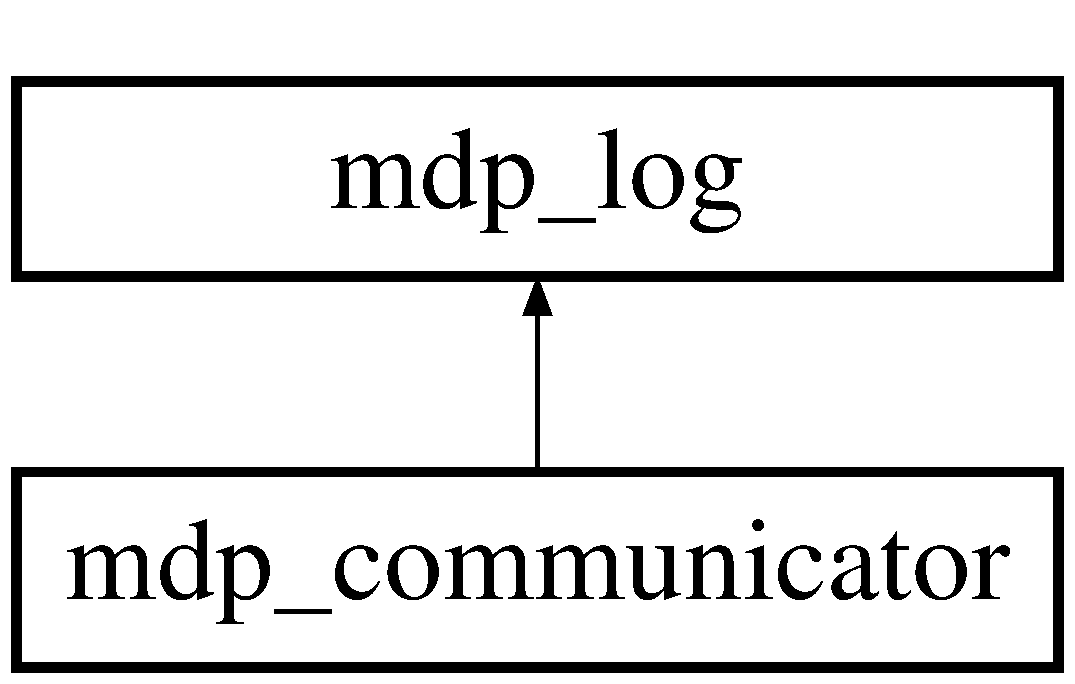
\includegraphics[height=2cm]{classmdp__log}
\end{center}
\end{figure}
\subsection*{Public Member Functions}
\begin{DoxyCompactItemize}
\item 
void \hyperlink{classmdp__log_a0e85794c9c7fdaf944eb70d1f2c0ecc5}{abort} ()
\item 
void \hyperlink{classmdp__log_a368a098416aa38fa3395607848a2c5f1}{set\_\-level} (int i)
\item 
\hyperlink{classmdp__log_a76a398101c2618249099be4fda3ce26c}{mdp\_\-log} ()
\item 
void \hyperlink{classmdp__log_a8e468b9b08d5008bbf87207a0184c809}{connect} (ostream \&os1)
\item 
void \hyperlink{classmdp__log_a9f9fbc3647e989231c4016179c2932d3}{connect} (ofstream \&os2)
\item 
void \hyperlink{classmdp__log_a675c488f1e494a9bd3a7466b300ec09a}{error\_\-message} (string s, string file, int line)
\item 
void \hyperlink{classmdp__log_a7fac0134af18caa8311bbf3118b82df1}{begin\_\-function} (string s)
\item 
void \hyperlink{classmdp__log_aeb82bba50423232fe8ad3a37ed65799d}{end\_\-function} (string s)
\item 
{\footnotesize template$<$class T $>$ }\\\hyperlink{classmdp__log}{mdp\_\-log} \& \hyperlink{classmdp__log_aa60825a5c02a42c5d1688a60d8da7516}{operator$<$$<$} (const T x)
\end{DoxyCompactItemize}
\subsection*{Public Attributes}
\begin{DoxyCompactItemize}
\item 
bool \hyperlink{classmdp__log_a1330daef61266763f9a736300a1eac49}{print}
\end{DoxyCompactItemize}


\subsection{Detailed Description}
base class of class \hyperlink{classmdp__communicator}{mdp\_\-communicator} (DO NOT INSTANTIATE) \begin{DoxySeeAlso}{See also}
class \hyperlink{classmdp__communicator}{mdp\_\-communicator} 
\end{DoxySeeAlso}


\subsection{Constructor \& Destructor Documentation}
\hypertarget{classmdp__log_a76a398101c2618249099be4fda3ce26c}{
\index{mdp\_\-log@{mdp\_\-log}!mdp\_\-log@{mdp\_\-log}}
\index{mdp\_\-log@{mdp\_\-log}!mdp_log@{mdp\_\-log}}
\subsubsection[{mdp\_\-log}]{\setlength{\rightskip}{0pt plus 5cm}mdp\_\-log::mdp\_\-log ()\hspace{0.3cm}{\ttfamily  \mbox{[}inline\mbox{]}}}}
\label{classmdp__log_a76a398101c2618249099be4fda3ce26c}


\subsection{Member Function Documentation}
\hypertarget{classmdp__log_a0e85794c9c7fdaf944eb70d1f2c0ecc5}{
\index{mdp\_\-log@{mdp\_\-log}!abort@{abort}}
\index{abort@{abort}!mdp_log@{mdp\_\-log}}
\subsubsection[{abort}]{\setlength{\rightskip}{0pt plus 5cm}void mdp\_\-log::abort ()\hspace{0.3cm}{\ttfamily  \mbox{[}inline\mbox{]}}}}
\label{classmdp__log_a0e85794c9c7fdaf944eb70d1f2c0ecc5}


Reimplemented in \hyperlink{classmdp__communicator_aa601b7788f242a7f71b955a6bdf7e002}{mdp\_\-communicator}.\hypertarget{classmdp__log_a7fac0134af18caa8311bbf3118b82df1}{
\index{mdp\_\-log@{mdp\_\-log}!begin\_\-function@{begin\_\-function}}
\index{begin\_\-function@{begin\_\-function}!mdp_log@{mdp\_\-log}}
\subsubsection[{begin\_\-function}]{\setlength{\rightskip}{0pt plus 5cm}void mdp\_\-log::begin\_\-function (string {\em s})\hspace{0.3cm}{\ttfamily  \mbox{[}inline\mbox{]}}}}
\label{classmdp__log_a7fac0134af18caa8311bbf3118b82df1}
\hypertarget{classmdp__log_a9f9fbc3647e989231c4016179c2932d3}{
\index{mdp\_\-log@{mdp\_\-log}!connect@{connect}}
\index{connect@{connect}!mdp_log@{mdp\_\-log}}
\subsubsection[{connect}]{\setlength{\rightskip}{0pt plus 5cm}void mdp\_\-log::connect (ofstream \& {\em os2})\hspace{0.3cm}{\ttfamily  \mbox{[}inline\mbox{]}}}}
\label{classmdp__log_a9f9fbc3647e989231c4016179c2932d3}
\hypertarget{classmdp__log_a8e468b9b08d5008bbf87207a0184c809}{
\index{mdp\_\-log@{mdp\_\-log}!connect@{connect}}
\index{connect@{connect}!mdp_log@{mdp\_\-log}}
\subsubsection[{connect}]{\setlength{\rightskip}{0pt plus 5cm}void mdp\_\-log::connect (ostream \& {\em os1})\hspace{0.3cm}{\ttfamily  \mbox{[}inline\mbox{]}}}}
\label{classmdp__log_a8e468b9b08d5008bbf87207a0184c809}
\hypertarget{classmdp__log_aeb82bba50423232fe8ad3a37ed65799d}{
\index{mdp\_\-log@{mdp\_\-log}!end\_\-function@{end\_\-function}}
\index{end\_\-function@{end\_\-function}!mdp_log@{mdp\_\-log}}
\subsubsection[{end\_\-function}]{\setlength{\rightskip}{0pt plus 5cm}void mdp\_\-log::end\_\-function (string {\em s})\hspace{0.3cm}{\ttfamily  \mbox{[}inline\mbox{]}}}}
\label{classmdp__log_aeb82bba50423232fe8ad3a37ed65799d}
\hypertarget{classmdp__log_a675c488f1e494a9bd3a7466b300ec09a}{
\index{mdp\_\-log@{mdp\_\-log}!error\_\-message@{error\_\-message}}
\index{error\_\-message@{error\_\-message}!mdp_log@{mdp\_\-log}}
\subsubsection[{error\_\-message}]{\setlength{\rightskip}{0pt plus 5cm}void mdp\_\-log::error\_\-message (string {\em s}, \/  string {\em file}, \/  int {\em line})\hspace{0.3cm}{\ttfamily  \mbox{[}inline\mbox{]}}}}
\label{classmdp__log_a675c488f1e494a9bd3a7466b300ec09a}
\hypertarget{classmdp__log_aa60825a5c02a42c5d1688a60d8da7516}{
\index{mdp\_\-log@{mdp\_\-log}!operator$<$$<$@{operator$<$$<$}}
\index{operator$<$$<$@{operator$<$$<$}!mdp_log@{mdp\_\-log}}
\subsubsection[{operator$<$$<$}]{\setlength{\rightskip}{0pt plus 5cm}template$<$class T $>$ {\bf mdp\_\-log}\& mdp\_\-log::operator$<$$<$ (const T {\em x})\hspace{0.3cm}{\ttfamily  \mbox{[}inline\mbox{]}}}}
\label{classmdp__log_aa60825a5c02a42c5d1688a60d8da7516}
\hypertarget{classmdp__log_a368a098416aa38fa3395607848a2c5f1}{
\index{mdp\_\-log@{mdp\_\-log}!set\_\-level@{set\_\-level}}
\index{set\_\-level@{set\_\-level}!mdp_log@{mdp\_\-log}}
\subsubsection[{set\_\-level}]{\setlength{\rightskip}{0pt plus 5cm}void mdp\_\-log::set\_\-level (int {\em i})\hspace{0.3cm}{\ttfamily  \mbox{[}inline\mbox{]}}}}
\label{classmdp__log_a368a098416aa38fa3395607848a2c5f1}


\subsection{Member Data Documentation}
\hypertarget{classmdp__log_a1330daef61266763f9a736300a1eac49}{
\index{mdp\_\-log@{mdp\_\-log}!print@{print}}
\index{print@{print}!mdp_log@{mdp\_\-log}}
\subsubsection[{print}]{\setlength{\rightskip}{0pt plus 5cm}bool {\bf mdp\_\-log::print}}}
\label{classmdp__log_a1330daef61266763f9a736300a1eac49}


The documentation for this class was generated from the following file:\begin{DoxyCompactItemize}
\item 
/Users/mdipierro/fermiqcd/development/Libraries/\hyperlink{mdp__log_8h}{mdp\_\-log.h}\end{DoxyCompactItemize}

\hypertarget{classmdp__matrix}{
\section{mdp\_\-matrix Class Reference}
\label{classmdp__matrix}\index{mdp\_\-matrix@{mdp\_\-matrix}}
}
matrices of complex numbers  


{\tt \#include $<$mdp\_\-matrix.h$>$}

Collaboration diagram for mdp\_\-matrix:

\subsection{Detailed Description}
matrices of complex numbers 

Example: 

\footnotesize\begin{verbatim}
///    mdp_matrix A,B;
///    A.dimension(3,3);
///    A(0,0)=A(1,1)=A(2,2)=A(1,2)=1.0+I/2;
///    B=A+inv(A)+exp(A+5);
/// \end{verbatim}
\normalsize
 

The documentation for this class was generated from the following file:\begin{CompactItemize}
\item 
/Users/mdipierro/Desktop/SciDac/development/Libraries/\hyperlink{mdp__matrix_8h}{mdp\_\-matrix.h}\end{CompactItemize}

\hypertarget{classmdp__matrix__field}{
\section{mdp\_\-matrix\_\-field Class Reference}
\label{classmdp__matrix__field}\index{mdp\_\-matrix\_\-field@{mdp\_\-matrix\_\-field}}
}
a field of matrices  


{\tt \#include $<$mdp\_\-matrix\_\-field.h$>$}

Inherits \hyperlink{classmdp__field}{mdp\_\-field$<$ mdp\_\-complex $>$}.

Collaboration diagram for mdp\_\-matrix\_\-field:

\subsection{Detailed Description}
a field of matrices 

Example: 

\footnotesize\begin{verbatim}
///    int box[]={10,10,10};
///    mdp_lattice lattice(3,box);
///    mdp_matrix_field h(lattice,5,5);
///    mdp_site x(lattice);
///    forallsites(x)
///       h(x)=lattice.random(x).SU(5);
/// \end{verbatim}
\normalsize
 

The documentation for this class was generated from the following file:\begin{CompactItemize}
\item 
/Users/mdipierro/Desktop/SciDac/development/Libraries/\hyperlink{mdp__matrix__field_8h}{mdp\_\-matrix\_\-field.h}\end{CompactItemize}

\hypertarget{classmdp__measure}{
\section{mdp\_\-measure Class Reference}
\label{classmdp__measure}\index{mdp\_\-measure@{mdp\_\-measure}}
}
implements error propagation  


{\tt \#include $<$mdp\_\-measure.h$>$}



\subsection{Detailed Description}
implements error propagation 

Example: 

\footnotesize\begin{verbatim}
///    mdp_measure m;
///    // store 10 measurements
///    for(int i=0; i<10; i++) 
///       m << 3.0+mdp_random.gaussian(2.0);
///    m=sin(exp(m)+m);
///    cout << m.getmean() << "+/-" << m.geterr() << endl;
/// \end{verbatim}
\normalsize
 Assumes gaussian error propagation 

The documentation for this class was generated from the following file:\begin{CompactItemize}
\item 
/Users/mdipierro/Desktop/SciDac/development/Libraries/\hyperlink{mdp__measure_8h}{mdp\_\-measure.h}\end{CompactItemize}

\hypertarget{classmdp__nmatrix__field}{
\section{mdp\_\-nmatrix\_\-field Class Reference}
\label{classmdp__nmatrix__field}\index{mdp\_\-nmatrix\_\-field@{mdp\_\-nmatrix\_\-field}}
}


field of vectors of matrices  


{\ttfamily \#include $<$mdp\_\-nmatrix\_\-field.h$>$}Inheritance diagram for mdp\_\-nmatrix\_\-field::\begin{figure}[H]
\begin{center}
\leavevmode
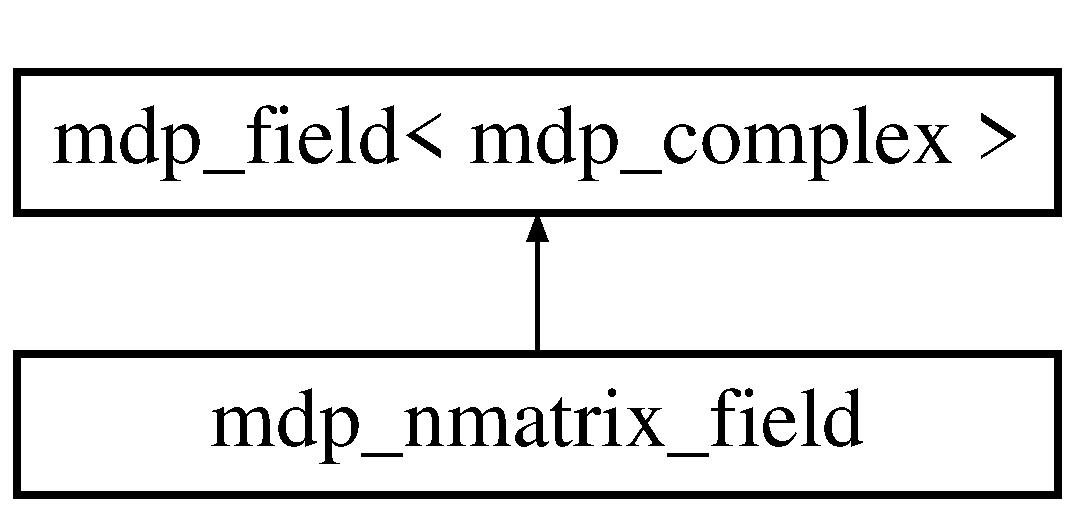
\includegraphics[height=2cm]{classmdp__nmatrix__field}
\end{center}
\end{figure}
\subsection*{Public Member Functions}
\begin{DoxyCompactItemize}
\item 
\hyperlink{classmdp__nmatrix__field_a2431fcb07b72317d2bf87e46ddad80b1}{mdp\_\-nmatrix\_\-field} ()
\item 
\hyperlink{classmdp__nmatrix__field_a8a3db6bfa6ffc2a5679c24f3e297e0c4}{mdp\_\-nmatrix\_\-field} (\hyperlink{classmdp__nmatrix__field}{mdp\_\-nmatrix\_\-field} \&field)
\item 
\hyperlink{classmdp__nmatrix__field_a10d00272d103d471a1cd9e5921d39419}{mdp\_\-nmatrix\_\-field} (\hyperlink{classmdp__lattice}{mdp\_\-lattice} \&a, int n, int i, int j)
\begin{DoxyCompactList}\small\item\em declares a field object that at each site as vector of n ixj matrices \item\end{DoxyCompactList}\item 
void \hyperlink{classmdp__nmatrix__field_ad8803e7b0f9a755329a1d7335ac0c019}{allocate\_\-mdp\_\-nmatrix\_\-field} (\hyperlink{classmdp__lattice}{mdp\_\-lattice} \&a, int n, int i, int j)
\begin{DoxyCompactList}\small\item\em dynamically allocates a field object that at each site as vector of n ixj matrices \item\end{DoxyCompactList}\item 
\hyperlink{classmdp__matrix}{mdp\_\-matrix} \hyperlink{classmdp__nmatrix__field_a389126da9ddf86d42b27d4d9d20245f8}{operator()} (\hyperlink{classmdp__site}{mdp\_\-site} x, int n)
\begin{DoxyCompactList}\small\item\em returns the n-\/th matrix stored at site x \item\end{DoxyCompactList}\item 
\hyperlink{classmdp__complex}{mdp\_\-complex} \& \hyperlink{classmdp__nmatrix__field_ab166e6abe76fcafd63dec9739da8324c}{operator()} (\hyperlink{classmdp__site}{mdp\_\-site} x, int n, int i, int j)
\begin{DoxyCompactList}\small\item\em returns the (i,j) component of the n-\/th matrix stored at site x \item\end{DoxyCompactList}\item 
const \hyperlink{classmdp__complex}{mdp\_\-complex} \& \hyperlink{classmdp__nmatrix__field_a4898cffa6a8e35bece4ed99a49499f3f}{operator()} (\hyperlink{classmdp__site}{mdp\_\-site} x, int n, int i, int j) const 
\end{DoxyCompactItemize}
\subsection*{Public Attributes}
\begin{DoxyCompactItemize}
\item 
\hyperlink{mdp__global__vars_8h_a91ad9478d81a7aaf2593e8d9c3d06a14}{uint} \hyperlink{classmdp__nmatrix__field_a6166f4d394efa361e3fa9552506c7c36}{rows}
\item 
\hyperlink{mdp__global__vars_8h_a91ad9478d81a7aaf2593e8d9c3d06a14}{uint} \hyperlink{classmdp__nmatrix__field_aaa3de1fa235579a53d5b4a3bc1ef504e}{columns}
\item 
\hyperlink{mdp__global__vars_8h_a91ad9478d81a7aaf2593e8d9c3d06a14}{uint} \hyperlink{classmdp__nmatrix__field_a7ace5d4385ddb2f67a8f1c5e65fbf22e}{matrices}
\item 
\hyperlink{mdp__global__vars_8h_a91ad9478d81a7aaf2593e8d9c3d06a14}{uint} \hyperlink{classmdp__nmatrix__field_a3f49b21188df1a14427384d3501b8926}{imax}
\item 
\hyperlink{mdp__global__vars_8h_a91ad9478d81a7aaf2593e8d9c3d06a14}{uint} \hyperlink{classmdp__nmatrix__field_acc8ab22ea97de1a94f6e3abe818cbafa}{imax2}
\end{DoxyCompactItemize}


\subsection{Detailed Description}
field of vectors of matrices Example: \begin{DoxyVerb}
///    int box[]={10,10,10};
///    mdp_lattice lattice(3,box);
///    mdp_nmatrix_field h(lattice,10,3,3);
///    mdp_site x(lattice);
///    forallsites(x)
///      for(int i=0; i<10; i++)
///        h(x,i)=lattice.random(x).SU(3);
/// \end{DoxyVerb}
 

\subsection{Constructor \& Destructor Documentation}
\hypertarget{classmdp__nmatrix__field_a2431fcb07b72317d2bf87e46ddad80b1}{
\index{mdp\_\-nmatrix\_\-field@{mdp\_\-nmatrix\_\-field}!mdp\_\-nmatrix\_\-field@{mdp\_\-nmatrix\_\-field}}
\index{mdp\_\-nmatrix\_\-field@{mdp\_\-nmatrix\_\-field}!mdp_nmatrix_field@{mdp\_\-nmatrix\_\-field}}
\subsubsection[{mdp\_\-nmatrix\_\-field}]{\setlength{\rightskip}{0pt plus 5cm}mdp\_\-nmatrix\_\-field::mdp\_\-nmatrix\_\-field ()\hspace{0.3cm}{\ttfamily  \mbox{[}inline\mbox{]}}}}
\label{classmdp__nmatrix__field_a2431fcb07b72317d2bf87e46ddad80b1}
\hypertarget{classmdp__nmatrix__field_a8a3db6bfa6ffc2a5679c24f3e297e0c4}{
\index{mdp\_\-nmatrix\_\-field@{mdp\_\-nmatrix\_\-field}!mdp\_\-nmatrix\_\-field@{mdp\_\-nmatrix\_\-field}}
\index{mdp\_\-nmatrix\_\-field@{mdp\_\-nmatrix\_\-field}!mdp_nmatrix_field@{mdp\_\-nmatrix\_\-field}}
\subsubsection[{mdp\_\-nmatrix\_\-field}]{\setlength{\rightskip}{0pt plus 5cm}mdp\_\-nmatrix\_\-field::mdp\_\-nmatrix\_\-field ({\bf mdp\_\-nmatrix\_\-field} \& {\em field})\hspace{0.3cm}{\ttfamily  \mbox{[}inline\mbox{]}}}}
\label{classmdp__nmatrix__field_a8a3db6bfa6ffc2a5679c24f3e297e0c4}
\hypertarget{classmdp__nmatrix__field_a10d00272d103d471a1cd9e5921d39419}{
\index{mdp\_\-nmatrix\_\-field@{mdp\_\-nmatrix\_\-field}!mdp\_\-nmatrix\_\-field@{mdp\_\-nmatrix\_\-field}}
\index{mdp\_\-nmatrix\_\-field@{mdp\_\-nmatrix\_\-field}!mdp_nmatrix_field@{mdp\_\-nmatrix\_\-field}}
\subsubsection[{mdp\_\-nmatrix\_\-field}]{\setlength{\rightskip}{0pt plus 5cm}mdp\_\-nmatrix\_\-field::mdp\_\-nmatrix\_\-field ({\bf mdp\_\-lattice} \& {\em a}, \/  int {\em n}, \/  int {\em i}, \/  int {\em j})\hspace{0.3cm}{\ttfamily  \mbox{[}inline\mbox{]}}}}
\label{classmdp__nmatrix__field_a10d00272d103d471a1cd9e5921d39419}


declares a field object that at each site as vector of n ixj matrices 

\subsection{Member Function Documentation}
\hypertarget{classmdp__nmatrix__field_ad8803e7b0f9a755329a1d7335ac0c019}{
\index{mdp\_\-nmatrix\_\-field@{mdp\_\-nmatrix\_\-field}!allocate\_\-mdp\_\-nmatrix\_\-field@{allocate\_\-mdp\_\-nmatrix\_\-field}}
\index{allocate\_\-mdp\_\-nmatrix\_\-field@{allocate\_\-mdp\_\-nmatrix\_\-field}!mdp_nmatrix_field@{mdp\_\-nmatrix\_\-field}}
\subsubsection[{allocate\_\-mdp\_\-nmatrix\_\-field}]{\setlength{\rightskip}{0pt plus 5cm}void mdp\_\-nmatrix\_\-field::allocate\_\-mdp\_\-nmatrix\_\-field ({\bf mdp\_\-lattice} \& {\em a}, \/  int {\em n}, \/  int {\em i}, \/  int {\em j})\hspace{0.3cm}{\ttfamily  \mbox{[}inline\mbox{]}}}}
\label{classmdp__nmatrix__field_ad8803e7b0f9a755329a1d7335ac0c019}


dynamically allocates a field object that at each site as vector of n ixj matrices \hypertarget{classmdp__nmatrix__field_a4898cffa6a8e35bece4ed99a49499f3f}{
\index{mdp\_\-nmatrix\_\-field@{mdp\_\-nmatrix\_\-field}!operator()@{operator()}}
\index{operator()@{operator()}!mdp_nmatrix_field@{mdp\_\-nmatrix\_\-field}}
\subsubsection[{operator()}]{\setlength{\rightskip}{0pt plus 5cm}const {\bf mdp\_\-complex}\& mdp\_\-nmatrix\_\-field::operator() ({\bf mdp\_\-site} {\em x}, \/  int {\em n}, \/  int {\em i}, \/  int {\em j}) const\hspace{0.3cm}{\ttfamily  \mbox{[}inline\mbox{]}}}}
\label{classmdp__nmatrix__field_a4898cffa6a8e35bece4ed99a49499f3f}
\hypertarget{classmdp__nmatrix__field_ab166e6abe76fcafd63dec9739da8324c}{
\index{mdp\_\-nmatrix\_\-field@{mdp\_\-nmatrix\_\-field}!operator()@{operator()}}
\index{operator()@{operator()}!mdp_nmatrix_field@{mdp\_\-nmatrix\_\-field}}
\subsubsection[{operator()}]{\setlength{\rightskip}{0pt plus 5cm}{\bf mdp\_\-complex}\& mdp\_\-nmatrix\_\-field::operator() ({\bf mdp\_\-site} {\em x}, \/  int {\em n}, \/  int {\em i}, \/  int {\em j})\hspace{0.3cm}{\ttfamily  \mbox{[}inline\mbox{]}}}}
\label{classmdp__nmatrix__field_ab166e6abe76fcafd63dec9739da8324c}


returns the (i,j) component of the n-\/th matrix stored at site x \hypertarget{classmdp__nmatrix__field_a389126da9ddf86d42b27d4d9d20245f8}{
\index{mdp\_\-nmatrix\_\-field@{mdp\_\-nmatrix\_\-field}!operator()@{operator()}}
\index{operator()@{operator()}!mdp_nmatrix_field@{mdp\_\-nmatrix\_\-field}}
\subsubsection[{operator()}]{\setlength{\rightskip}{0pt plus 5cm}{\bf mdp\_\-matrix} mdp\_\-nmatrix\_\-field::operator() ({\bf mdp\_\-site} {\em x}, \/  int {\em n})\hspace{0.3cm}{\ttfamily  \mbox{[}inline\mbox{]}}}}
\label{classmdp__nmatrix__field_a389126da9ddf86d42b27d4d9d20245f8}


returns the n-\/th matrix stored at site x 

Reimplemented from \hyperlink{classmdp__field_a9eec94ee723253a196ccc4677832b4a0}{mdp\_\-field$<$ mdp\_\-complex $>$}.

\subsection{Member Data Documentation}
\hypertarget{classmdp__nmatrix__field_aaa3de1fa235579a53d5b4a3bc1ef504e}{
\index{mdp\_\-nmatrix\_\-field@{mdp\_\-nmatrix\_\-field}!columns@{columns}}
\index{columns@{columns}!mdp_nmatrix_field@{mdp\_\-nmatrix\_\-field}}
\subsubsection[{columns}]{\setlength{\rightskip}{0pt plus 5cm}{\bf uint} {\bf mdp\_\-nmatrix\_\-field::columns}}}
\label{classmdp__nmatrix__field_aaa3de1fa235579a53d5b4a3bc1ef504e}
\hypertarget{classmdp__nmatrix__field_a3f49b21188df1a14427384d3501b8926}{
\index{mdp\_\-nmatrix\_\-field@{mdp\_\-nmatrix\_\-field}!imax@{imax}}
\index{imax@{imax}!mdp_nmatrix_field@{mdp\_\-nmatrix\_\-field}}
\subsubsection[{imax}]{\setlength{\rightskip}{0pt plus 5cm}{\bf uint} {\bf mdp\_\-nmatrix\_\-field::imax}}}
\label{classmdp__nmatrix__field_a3f49b21188df1a14427384d3501b8926}
\hypertarget{classmdp__nmatrix__field_acc8ab22ea97de1a94f6e3abe818cbafa}{
\index{mdp\_\-nmatrix\_\-field@{mdp\_\-nmatrix\_\-field}!imax2@{imax2}}
\index{imax2@{imax2}!mdp_nmatrix_field@{mdp\_\-nmatrix\_\-field}}
\subsubsection[{imax2}]{\setlength{\rightskip}{0pt plus 5cm}{\bf uint} {\bf mdp\_\-nmatrix\_\-field::imax2}}}
\label{classmdp__nmatrix__field_acc8ab22ea97de1a94f6e3abe818cbafa}
\hypertarget{classmdp__nmatrix__field_a7ace5d4385ddb2f67a8f1c5e65fbf22e}{
\index{mdp\_\-nmatrix\_\-field@{mdp\_\-nmatrix\_\-field}!matrices@{matrices}}
\index{matrices@{matrices}!mdp_nmatrix_field@{mdp\_\-nmatrix\_\-field}}
\subsubsection[{matrices}]{\setlength{\rightskip}{0pt plus 5cm}{\bf uint} {\bf mdp\_\-nmatrix\_\-field::matrices}}}
\label{classmdp__nmatrix__field_a7ace5d4385ddb2f67a8f1c5e65fbf22e}
\hypertarget{classmdp__nmatrix__field_a6166f4d394efa361e3fa9552506c7c36}{
\index{mdp\_\-nmatrix\_\-field@{mdp\_\-nmatrix\_\-field}!rows@{rows}}
\index{rows@{rows}!mdp_nmatrix_field@{mdp\_\-nmatrix\_\-field}}
\subsubsection[{rows}]{\setlength{\rightskip}{0pt plus 5cm}{\bf uint} {\bf mdp\_\-nmatrix\_\-field::rows}}}
\label{classmdp__nmatrix__field_a6166f4d394efa361e3fa9552506c7c36}


The documentation for this class was generated from the following file:\begin{DoxyCompactItemize}
\item 
/Users/mdipierro/fermiqcd/development/Libraries/\hyperlink{mdp__nmatrix__field_8h}{mdp\_\-nmatrix\_\-field.h}\end{DoxyCompactItemize}

\hypertarget{classmdp__nvector__field}{
\section{mdp\_\-nvector\_\-field Class Reference}
\label{classmdp__nvector__field}\index{mdp\_\-nvector\_\-field@{mdp\_\-nvector\_\-field}}
}
field of vectors of vectors (DEPRECATED)  


{\tt \#include $<$mdp\_\-nvector\_\-field.h$>$}

Inherits \hyperlink{classmdp__field}{mdp\_\-field$<$ mdp\_\-complex $>$}.

Collaboration diagram for mdp\_\-nvector\_\-field:\subsection*{Public Member Functions}
\begin{CompactItemize}
\item 
\hypertarget{classmdp__nvector__field_fddf6115e2d88a72727d66949436d8ca}{
\hyperlink{classmdp__matrix}{mdp\_\-matrix} \hyperlink{classmdp__nvector__field_fddf6115e2d88a72727d66949436d8ca}{operator()} (\hyperlink{classmdp__site}{mdp\_\-site} x, int n)}
\label{classmdp__nvector__field_fddf6115e2d88a72727d66949436d8ca}

\begin{CompactList}\small\item\em returns component i of the vector of objects T stored at site x \item\end{CompactList}\end{CompactItemize}


\subsection{Detailed Description}
field of vectors of vectors (DEPRECATED) 

The documentation for this class was generated from the following file:\begin{CompactItemize}
\item 
/Users/mdipierro/Desktop/SciDac/development/Libraries/\hyperlink{mdp__nvector__field_8h}{mdp\_\-nvector\_\-field.h}\end{CompactItemize}

\hypertarget{classmdp__postscript}{
\section{mdp\_\-postscript Class Reference}
\label{classmdp__postscript}\index{mdp\_\-postscript@{mdp\_\-postscript}}
}


to output and draw in postscript  


{\ttfamily \#include $<$mdp\_\-postscript.h$>$}\subsection*{Public Types}
\begin{DoxyCompactItemize}
\item 
enum \{ \hyperlink{classmdp__postscript_a9a7e58c0e001105f4fe6d86a0a11348fa8266db73d3c5c06b4c4e8fdb9c4c38c0}{BOLD} = 10
 \}
\end{DoxyCompactItemize}
\subsection*{Public Member Functions}
\begin{DoxyCompactItemize}
\item 
\hyperlink{classmdp__postscript_a30a69ecea648f202d533b02c8f21f119}{mdp\_\-postscript} ()
\item 
\hyperlink{classmdp__postscript_a94b381b18ec3bce5ab2ac9f0f33dcb53}{mdp\_\-postscript} (char filename\mbox{[}$\,$\mbox{]})
\item 
virtual \hyperlink{classmdp__postscript_a3a46d2757dc2954f970987cb3bea2784}{$\sim$mdp\_\-postscript} ()
\item 
FILE $\ast$ \hyperlink{classmdp__postscript_a2c2ab911f52c386532b769dda793dcdc}{open} (char filename\mbox{[}$\,$\mbox{]})
\item 
void \hyperlink{classmdp__postscript_af41a3aa09549d5acb2b5e9a098f69089}{close} ()
\item 
void \hyperlink{classmdp__postscript_af62e32c26c084b83e1a6c318767f2192}{size} (float x0, float y0, float x1, float y1)
\item 
void \hyperlink{classmdp__postscript_a99a00f3641062e5beef501f07baa7785}{line} (float x0, float y0, float x1, float y1)
\item 
void \hyperlink{classmdp__postscript_aa44192cb071b678edb48adb39053a396}{box} (float x0, float y0, float x1, float y1, int fill=0)
\item 
void \hyperlink{classmdp__postscript_a56092f2141d3d1b0cc4afd333bed5e1e}{arc} (float x0, float y0, float r, float \hyperlink{classmdp__postscript_aca4cc1e7bee7fa702c643bdb1c69d6d0}{alpha}, float beta)
\item 
void \hyperlink{classmdp__postscript_abfa4c3e6cfd19b2ddb190ca9a5f2df02}{circle} (float x0, float y0, float r, int fill=0)
\item 
void \hyperlink{classmdp__postscript_a416d831d67bb6db2512f3e819eee8bf3}{pen} (float size)
\item 
void \hyperlink{classmdp__postscript_ae4c5ce5c229ad7cfef67a689c77acac3}{color} (float r, float g, float b)
\item 
void \hyperlink{classmdp__postscript_a296dff78ebec7c38e3c39d97d3743172}{font} (const char $\ast$text, int size)
\item 
void \hyperlink{classmdp__postscript_a0c67b14a365475f3b5b04d3d033cc4c4}{print} (float x0, float y0, char text\mbox{[}$\,$\mbox{]})
\end{DoxyCompactItemize}
\subsection*{Public Attributes}
\begin{DoxyCompactItemize}
\item 
FILE $\ast$ \hyperlink{classmdp__postscript_a0d313085dea47b974fdd18ecb26622f1}{fp}
\item 
float \hyperlink{classmdp__postscript_a535f3c0036f5d89c139b003c0e909eed}{X0}
\item 
float \hyperlink{classmdp__postscript_acce7497a1e20c1c98708b95041faa274}{Y0}
\item 
float \hyperlink{classmdp__postscript_a5c27b031c6f79593b476dfa6a69e146f}{Z0}
\item 
float \hyperlink{classmdp__postscript_a71402d65d648f4c878dfe5eb74679efa}{X1}
\item 
float \hyperlink{classmdp__postscript_a812d1985306950bed3a2d858e8236b5b}{Y1}
\item 
float \hyperlink{classmdp__postscript_ac512287091dcecae1a549d005083554f}{Z1}
\item 
float \hyperlink{classmdp__postscript_a3160a1940a9fa4e99a0b138bc88769e9}{c0}
\item 
float \hyperlink{classmdp__postscript_a92dc6ce50f362fe93a1981b9a126073a}{c1}
\item 
float \hyperlink{classmdp__postscript_a26f42cf1f154707c463ecdd3f19f568f}{c2}
\item 
float \hyperlink{classmdp__postscript_ae0bd063ba78d27ad7ce541e78f512d3a}{scale}
\item 
float \hyperlink{classmdp__postscript_aca4cc1e7bee7fa702c643bdb1c69d6d0}{alpha}
\end{DoxyCompactItemize}


\subsection{Detailed Description}
to output and draw in postscript Example: \begin{DoxyVerb}
///    mdp_postscript ps("test.ps");
///    ps.color(0.2,0.2,0.7);
///    ps.line(0,0,  5,5);
///    ps.print(5,5,"a line from (0,0) to here");
/// \end{DoxyVerb}
 

\subsection{Member Enumeration Documentation}
\hypertarget{classmdp__postscript_a9a7e58c0e001105f4fe6d86a0a11348f}{
\subsubsection[{"@5}]{\setlength{\rightskip}{0pt plus 5cm}anonymous enum}}
\label{classmdp__postscript_a9a7e58c0e001105f4fe6d86a0a11348f}
\begin{Desc}
\item[Enumerator: ]\par
\begin{description}
\index{BOLD@{BOLD}!mdp\_\-postscript@{mdp\_\-postscript}}\index{mdp\_\-postscript@{mdp\_\-postscript}!BOLD@{BOLD}}\item[{\em 
\hypertarget{classmdp__postscript_a9a7e58c0e001105f4fe6d86a0a11348fa8266db73d3c5c06b4c4e8fdb9c4c38c0}{
BOLD}
\label{classmdp__postscript_a9a7e58c0e001105f4fe6d86a0a11348fa8266db73d3c5c06b4c4e8fdb9c4c38c0}
}]\end{description}
\end{Desc}



\subsection{Constructor \& Destructor Documentation}
\hypertarget{classmdp__postscript_a30a69ecea648f202d533b02c8f21f119}{
\index{mdp\_\-postscript@{mdp\_\-postscript}!mdp\_\-postscript@{mdp\_\-postscript}}
\index{mdp\_\-postscript@{mdp\_\-postscript}!mdp_postscript@{mdp\_\-postscript}}
\subsubsection[{mdp\_\-postscript}]{\setlength{\rightskip}{0pt plus 5cm}mdp\_\-postscript::mdp\_\-postscript ()\hspace{0.3cm}{\ttfamily  \mbox{[}inline\mbox{]}}}}
\label{classmdp__postscript_a30a69ecea648f202d533b02c8f21f119}
\hypertarget{classmdp__postscript_a94b381b18ec3bce5ab2ac9f0f33dcb53}{
\index{mdp\_\-postscript@{mdp\_\-postscript}!mdp\_\-postscript@{mdp\_\-postscript}}
\index{mdp\_\-postscript@{mdp\_\-postscript}!mdp_postscript@{mdp\_\-postscript}}
\subsubsection[{mdp\_\-postscript}]{\setlength{\rightskip}{0pt plus 5cm}mdp\_\-postscript::mdp\_\-postscript (char {\em filename}\mbox{[}$\,$\mbox{]})\hspace{0.3cm}{\ttfamily  \mbox{[}inline\mbox{]}}}}
\label{classmdp__postscript_a94b381b18ec3bce5ab2ac9f0f33dcb53}
\hypertarget{classmdp__postscript_a3a46d2757dc2954f970987cb3bea2784}{
\index{mdp\_\-postscript@{mdp\_\-postscript}!$\sim$mdp\_\-postscript@{$\sim$mdp\_\-postscript}}
\index{$\sim$mdp\_\-postscript@{$\sim$mdp\_\-postscript}!mdp_postscript@{mdp\_\-postscript}}
\subsubsection[{$\sim$mdp\_\-postscript}]{\setlength{\rightskip}{0pt plus 5cm}virtual mdp\_\-postscript::$\sim$mdp\_\-postscript ()\hspace{0.3cm}{\ttfamily  \mbox{[}inline, virtual\mbox{]}}}}
\label{classmdp__postscript_a3a46d2757dc2954f970987cb3bea2784}


\subsection{Member Function Documentation}
\hypertarget{classmdp__postscript_a56092f2141d3d1b0cc4afd333bed5e1e}{
\index{mdp\_\-postscript@{mdp\_\-postscript}!arc@{arc}}
\index{arc@{arc}!mdp_postscript@{mdp\_\-postscript}}
\subsubsection[{arc}]{\setlength{\rightskip}{0pt plus 5cm}void mdp\_\-postscript::arc (float {\em x0}, \/  float {\em y0}, \/  float {\em r}, \/  float {\em alpha}, \/  float {\em beta})\hspace{0.3cm}{\ttfamily  \mbox{[}inline\mbox{]}}}}
\label{classmdp__postscript_a56092f2141d3d1b0cc4afd333bed5e1e}
\hypertarget{classmdp__postscript_aa44192cb071b678edb48adb39053a396}{
\index{mdp\_\-postscript@{mdp\_\-postscript}!box@{box}}
\index{box@{box}!mdp_postscript@{mdp\_\-postscript}}
\subsubsection[{box}]{\setlength{\rightskip}{0pt plus 5cm}void mdp\_\-postscript::box (float {\em x0}, \/  float {\em y0}, \/  float {\em x1}, \/  float {\em y1}, \/  int {\em fill} = {\ttfamily 0})\hspace{0.3cm}{\ttfamily  \mbox{[}inline\mbox{]}}}}
\label{classmdp__postscript_aa44192cb071b678edb48adb39053a396}
\hypertarget{classmdp__postscript_abfa4c3e6cfd19b2ddb190ca9a5f2df02}{
\index{mdp\_\-postscript@{mdp\_\-postscript}!circle@{circle}}
\index{circle@{circle}!mdp_postscript@{mdp\_\-postscript}}
\subsubsection[{circle}]{\setlength{\rightskip}{0pt plus 5cm}void mdp\_\-postscript::circle (float {\em x0}, \/  float {\em y0}, \/  float {\em r}, \/  int {\em fill} = {\ttfamily 0})\hspace{0.3cm}{\ttfamily  \mbox{[}inline\mbox{]}}}}
\label{classmdp__postscript_abfa4c3e6cfd19b2ddb190ca9a5f2df02}
\hypertarget{classmdp__postscript_af41a3aa09549d5acb2b5e9a098f69089}{
\index{mdp\_\-postscript@{mdp\_\-postscript}!close@{close}}
\index{close@{close}!mdp_postscript@{mdp\_\-postscript}}
\subsubsection[{close}]{\setlength{\rightskip}{0pt plus 5cm}void mdp\_\-postscript::close ()\hspace{0.3cm}{\ttfamily  \mbox{[}inline\mbox{]}}}}
\label{classmdp__postscript_af41a3aa09549d5acb2b5e9a098f69089}
\hypertarget{classmdp__postscript_ae4c5ce5c229ad7cfef67a689c77acac3}{
\index{mdp\_\-postscript@{mdp\_\-postscript}!color@{color}}
\index{color@{color}!mdp_postscript@{mdp\_\-postscript}}
\subsubsection[{color}]{\setlength{\rightskip}{0pt plus 5cm}void mdp\_\-postscript::color (float {\em r}, \/  float {\em g}, \/  float {\em b})\hspace{0.3cm}{\ttfamily  \mbox{[}inline\mbox{]}}}}
\label{classmdp__postscript_ae4c5ce5c229ad7cfef67a689c77acac3}
\hypertarget{classmdp__postscript_a296dff78ebec7c38e3c39d97d3743172}{
\index{mdp\_\-postscript@{mdp\_\-postscript}!font@{font}}
\index{font@{font}!mdp_postscript@{mdp\_\-postscript}}
\subsubsection[{font}]{\setlength{\rightskip}{0pt plus 5cm}void mdp\_\-postscript::font (const char $\ast$ {\em text}, \/  int {\em size})\hspace{0.3cm}{\ttfamily  \mbox{[}inline\mbox{]}}}}
\label{classmdp__postscript_a296dff78ebec7c38e3c39d97d3743172}
\hypertarget{classmdp__postscript_a99a00f3641062e5beef501f07baa7785}{
\index{mdp\_\-postscript@{mdp\_\-postscript}!line@{line}}
\index{line@{line}!mdp_postscript@{mdp\_\-postscript}}
\subsubsection[{line}]{\setlength{\rightskip}{0pt plus 5cm}void mdp\_\-postscript::line (float {\em x0}, \/  float {\em y0}, \/  float {\em x1}, \/  float {\em y1})\hspace{0.3cm}{\ttfamily  \mbox{[}inline\mbox{]}}}}
\label{classmdp__postscript_a99a00f3641062e5beef501f07baa7785}
\hypertarget{classmdp__postscript_a2c2ab911f52c386532b769dda793dcdc}{
\index{mdp\_\-postscript@{mdp\_\-postscript}!open@{open}}
\index{open@{open}!mdp_postscript@{mdp\_\-postscript}}
\subsubsection[{open}]{\setlength{\rightskip}{0pt plus 5cm}FILE$\ast$ mdp\_\-postscript::open (char {\em filename}\mbox{[}$\,$\mbox{]})\hspace{0.3cm}{\ttfamily  \mbox{[}inline\mbox{]}}}}
\label{classmdp__postscript_a2c2ab911f52c386532b769dda793dcdc}
\hypertarget{classmdp__postscript_a416d831d67bb6db2512f3e819eee8bf3}{
\index{mdp\_\-postscript@{mdp\_\-postscript}!pen@{pen}}
\index{pen@{pen}!mdp_postscript@{mdp\_\-postscript}}
\subsubsection[{pen}]{\setlength{\rightskip}{0pt plus 5cm}void mdp\_\-postscript::pen (float {\em size})\hspace{0.3cm}{\ttfamily  \mbox{[}inline\mbox{]}}}}
\label{classmdp__postscript_a416d831d67bb6db2512f3e819eee8bf3}
\hypertarget{classmdp__postscript_a0c67b14a365475f3b5b04d3d033cc4c4}{
\index{mdp\_\-postscript@{mdp\_\-postscript}!print@{print}}
\index{print@{print}!mdp_postscript@{mdp\_\-postscript}}
\subsubsection[{print}]{\setlength{\rightskip}{0pt plus 5cm}void mdp\_\-postscript::print (float {\em x0}, \/  float {\em y0}, \/  char {\em text}\mbox{[}$\,$\mbox{]})\hspace{0.3cm}{\ttfamily  \mbox{[}inline\mbox{]}}}}
\label{classmdp__postscript_a0c67b14a365475f3b5b04d3d033cc4c4}
\hypertarget{classmdp__postscript_af62e32c26c084b83e1a6c318767f2192}{
\index{mdp\_\-postscript@{mdp\_\-postscript}!size@{size}}
\index{size@{size}!mdp_postscript@{mdp\_\-postscript}}
\subsubsection[{size}]{\setlength{\rightskip}{0pt plus 5cm}void mdp\_\-postscript::size (float {\em x0}, \/  float {\em y0}, \/  float {\em x1}, \/  float {\em y1})\hspace{0.3cm}{\ttfamily  \mbox{[}inline\mbox{]}}}}
\label{classmdp__postscript_af62e32c26c084b83e1a6c318767f2192}


\subsection{Member Data Documentation}
\hypertarget{classmdp__postscript_aca4cc1e7bee7fa702c643bdb1c69d6d0}{
\index{mdp\_\-postscript@{mdp\_\-postscript}!alpha@{alpha}}
\index{alpha@{alpha}!mdp_postscript@{mdp\_\-postscript}}
\subsubsection[{alpha}]{\setlength{\rightskip}{0pt plus 5cm}float {\bf mdp\_\-postscript::alpha}}}
\label{classmdp__postscript_aca4cc1e7bee7fa702c643bdb1c69d6d0}
\hypertarget{classmdp__postscript_a3160a1940a9fa4e99a0b138bc88769e9}{
\index{mdp\_\-postscript@{mdp\_\-postscript}!c0@{c0}}
\index{c0@{c0}!mdp_postscript@{mdp\_\-postscript}}
\subsubsection[{c0}]{\setlength{\rightskip}{0pt plus 5cm}float {\bf mdp\_\-postscript::c0}}}
\label{classmdp__postscript_a3160a1940a9fa4e99a0b138bc88769e9}
\hypertarget{classmdp__postscript_a92dc6ce50f362fe93a1981b9a126073a}{
\index{mdp\_\-postscript@{mdp\_\-postscript}!c1@{c1}}
\index{c1@{c1}!mdp_postscript@{mdp\_\-postscript}}
\subsubsection[{c1}]{\setlength{\rightskip}{0pt plus 5cm}float {\bf mdp\_\-postscript::c1}}}
\label{classmdp__postscript_a92dc6ce50f362fe93a1981b9a126073a}
\hypertarget{classmdp__postscript_a26f42cf1f154707c463ecdd3f19f568f}{
\index{mdp\_\-postscript@{mdp\_\-postscript}!c2@{c2}}
\index{c2@{c2}!mdp_postscript@{mdp\_\-postscript}}
\subsubsection[{c2}]{\setlength{\rightskip}{0pt plus 5cm}float {\bf mdp\_\-postscript::c2}}}
\label{classmdp__postscript_a26f42cf1f154707c463ecdd3f19f568f}
\hypertarget{classmdp__postscript_a0d313085dea47b974fdd18ecb26622f1}{
\index{mdp\_\-postscript@{mdp\_\-postscript}!fp@{fp}}
\index{fp@{fp}!mdp_postscript@{mdp\_\-postscript}}
\subsubsection[{fp}]{\setlength{\rightskip}{0pt plus 5cm}FILE$\ast$ {\bf mdp\_\-postscript::fp}}}
\label{classmdp__postscript_a0d313085dea47b974fdd18ecb26622f1}
\hypertarget{classmdp__postscript_ae0bd063ba78d27ad7ce541e78f512d3a}{
\index{mdp\_\-postscript@{mdp\_\-postscript}!scale@{scale}}
\index{scale@{scale}!mdp_postscript@{mdp\_\-postscript}}
\subsubsection[{scale}]{\setlength{\rightskip}{0pt plus 5cm}float {\bf mdp\_\-postscript::scale}}}
\label{classmdp__postscript_ae0bd063ba78d27ad7ce541e78f512d3a}
\hypertarget{classmdp__postscript_a535f3c0036f5d89c139b003c0e909eed}{
\index{mdp\_\-postscript@{mdp\_\-postscript}!X0@{X0}}
\index{X0@{X0}!mdp_postscript@{mdp\_\-postscript}}
\subsubsection[{X0}]{\setlength{\rightskip}{0pt plus 5cm}float {\bf mdp\_\-postscript::X0}}}
\label{classmdp__postscript_a535f3c0036f5d89c139b003c0e909eed}
\hypertarget{classmdp__postscript_a71402d65d648f4c878dfe5eb74679efa}{
\index{mdp\_\-postscript@{mdp\_\-postscript}!X1@{X1}}
\index{X1@{X1}!mdp_postscript@{mdp\_\-postscript}}
\subsubsection[{X1}]{\setlength{\rightskip}{0pt plus 5cm}float {\bf mdp\_\-postscript::X1}}}
\label{classmdp__postscript_a71402d65d648f4c878dfe5eb74679efa}
\hypertarget{classmdp__postscript_acce7497a1e20c1c98708b95041faa274}{
\index{mdp\_\-postscript@{mdp\_\-postscript}!Y0@{Y0}}
\index{Y0@{Y0}!mdp_postscript@{mdp\_\-postscript}}
\subsubsection[{Y0}]{\setlength{\rightskip}{0pt plus 5cm}float {\bf mdp\_\-postscript::Y0}}}
\label{classmdp__postscript_acce7497a1e20c1c98708b95041faa274}
\hypertarget{classmdp__postscript_a812d1985306950bed3a2d858e8236b5b}{
\index{mdp\_\-postscript@{mdp\_\-postscript}!Y1@{Y1}}
\index{Y1@{Y1}!mdp_postscript@{mdp\_\-postscript}}
\subsubsection[{Y1}]{\setlength{\rightskip}{0pt plus 5cm}float {\bf mdp\_\-postscript::Y1}}}
\label{classmdp__postscript_a812d1985306950bed3a2d858e8236b5b}
\hypertarget{classmdp__postscript_a5c27b031c6f79593b476dfa6a69e146f}{
\index{mdp\_\-postscript@{mdp\_\-postscript}!Z0@{Z0}}
\index{Z0@{Z0}!mdp_postscript@{mdp\_\-postscript}}
\subsubsection[{Z0}]{\setlength{\rightskip}{0pt plus 5cm}float {\bf mdp\_\-postscript::Z0}}}
\label{classmdp__postscript_a5c27b031c6f79593b476dfa6a69e146f}
\hypertarget{classmdp__postscript_ac512287091dcecae1a549d005083554f}{
\index{mdp\_\-postscript@{mdp\_\-postscript}!Z1@{Z1}}
\index{Z1@{Z1}!mdp_postscript@{mdp\_\-postscript}}
\subsubsection[{Z1}]{\setlength{\rightskip}{0pt plus 5cm}float {\bf mdp\_\-postscript::Z1}}}
\label{classmdp__postscript_ac512287091dcecae1a549d005083554f}


The documentation for this class was generated from the following file:\begin{DoxyCompactItemize}
\item 
/Users/mdipierro/fermiqcd/development/Libraries/\hyperlink{mdp__postscript_8h}{mdp\_\-postscript.h}\end{DoxyCompactItemize}

\hypertarget{classmdp__prng}{
\section{mdp\_\-prng Class Reference}
\label{classmdp__prng}\index{mdp\_\-prng@{mdp\_\-prng}}
}


Marsaglia's random number generator (same as UKQCD).  


{\ttfamily \#include $<$mdp\_\-prng.h$>$}\subsection*{Public Member Functions}
\begin{DoxyCompactItemize}
\item 
float \hyperlink{classmdp__prng_a261360660403dcd1a76305a8644b6a2d}{plain} ()
\begin{DoxyCompactList}\small\item\em return a uniform random number in (0,1) \item\end{DoxyCompactList}\item 
void \hyperlink{classmdp__prng_a2a41d455e32ec21fce0c76f71bda801a}{initialize} (\hyperlink{mdp__global__vars_8h_aaa1ad9d0dcd2124aa5af0120d9954174}{mdp\_\-int} ijkl)
\item 
\hyperlink{classmdp__prng_a57739df3a7629078ca66dbfd7ded1b86}{mdp\_\-prng} (\hyperlink{mdp__global__vars_8h_aaa1ad9d0dcd2124aa5af0120d9954174}{mdp\_\-int} k=0)
\item 
float \hyperlink{classmdp__prng_adf372628df14ef01302472264a7f26d8}{gaussian} (float \hyperlink{fermiqcd__gamma__matrices_8h_ab20455955848cb6945fe37dda0a2ef40}{sigma}=1)
\begin{DoxyCompactList}\small\item\em returns a gaussian random number \item\end{DoxyCompactList}\item 
double \hyperlink{classmdp__prng_a2ba8807aa153b9b222d6d724da06dfdd}{distribution} (float($\ast$fp)(float, void $\ast$), void $\ast$a=0)
\begin{DoxyCompactList}\small\item\em draws a random float in (0,1) from a distribution using accept-\/reject \item\end{DoxyCompactList}\item 
\hyperlink{classmdp__matrix}{mdp\_\-matrix} \hyperlink{classmdp__prng_a348d0a778f0c1e3dd71e163bad950936}{SU} (int n)
\begin{DoxyCompactList}\small\item\em returns a random SU(n) matrix using Cabibbo-\/Marinari \item\end{DoxyCompactList}\item 
void \hyperlink{classmdp__prng_a6214a2e9ed4d3da1e61544501e710999}{skip} (int n)
\begin{DoxyCompactList}\small\item\em skip n numbers from the sequence \item\end{DoxyCompactList}\end{DoxyCompactItemize}


\subsection{Detailed Description}
Marsaglia's random number generator (same as UKQCD). You should not instantiate this class because:
\begin{DoxyItemize}
\item there is a global object mdp\_\-random
\item each field \char`\"{}lattice\char`\"{} has a parallel generator \char`\"{}lattice.random(x)\char`\"{} Example: \begin{DoxyVerb}
///    // print a uniform number in (0,1)
///    cout << mdp_random.plain() << endl;
///    // print a gaussian number
///    cout << mdp_random.gaussian() << endl;
///    // print a random SU(10) matrix
///    cout << mdp_random.SU(10) << endl;
/// \end{DoxyVerb}
 
\end{DoxyItemize}

\subsection{Constructor \& Destructor Documentation}
\hypertarget{classmdp__prng_a57739df3a7629078ca66dbfd7ded1b86}{
\index{mdp\_\-prng@{mdp\_\-prng}!mdp\_\-prng@{mdp\_\-prng}}
\index{mdp\_\-prng@{mdp\_\-prng}!mdp_prng@{mdp\_\-prng}}
\subsubsection[{mdp\_\-prng}]{\setlength{\rightskip}{0pt plus 5cm}mdp\_\-prng::mdp\_\-prng ({\bf mdp\_\-int} {\em k} = {\ttfamily 0})\hspace{0.3cm}{\ttfamily  \mbox{[}inline\mbox{]}}}}
\label{classmdp__prng_a57739df3a7629078ca66dbfd7ded1b86}


\subsection{Member Function Documentation}
\hypertarget{classmdp__prng_a2ba8807aa153b9b222d6d724da06dfdd}{
\index{mdp\_\-prng@{mdp\_\-prng}!distribution@{distribution}}
\index{distribution@{distribution}!mdp_prng@{mdp\_\-prng}}
\subsubsection[{distribution}]{\setlength{\rightskip}{0pt plus 5cm}double mdp\_\-prng::distribution (float($\ast$)(float, void $\ast$) {\em fp}, \/  void $\ast$ {\em a} = {\ttfamily 0})\hspace{0.3cm}{\ttfamily  \mbox{[}inline\mbox{]}}}}
\label{classmdp__prng_a2ba8807aa153b9b222d6d724da06dfdd}


draws a random float in (0,1) from a distribution using accept-\/reject \hypertarget{classmdp__prng_adf372628df14ef01302472264a7f26d8}{
\index{mdp\_\-prng@{mdp\_\-prng}!gaussian@{gaussian}}
\index{gaussian@{gaussian}!mdp_prng@{mdp\_\-prng}}
\subsubsection[{gaussian}]{\setlength{\rightskip}{0pt plus 5cm}float mdp\_\-prng::gaussian (float {\em sigma} = {\ttfamily 1})\hspace{0.3cm}{\ttfamily  \mbox{[}inline\mbox{]}}}}
\label{classmdp__prng_adf372628df14ef01302472264a7f26d8}


returns a gaussian random number \hypertarget{classmdp__prng_a2a41d455e32ec21fce0c76f71bda801a}{
\index{mdp\_\-prng@{mdp\_\-prng}!initialize@{initialize}}
\index{initialize@{initialize}!mdp_prng@{mdp\_\-prng}}
\subsubsection[{initialize}]{\setlength{\rightskip}{0pt plus 5cm}void mdp\_\-prng::initialize ({\bf mdp\_\-int} {\em ijkl})\hspace{0.3cm}{\ttfamily  \mbox{[}inline\mbox{]}}}}
\label{classmdp__prng_a2a41d455e32ec21fce0c76f71bda801a}
\hypertarget{classmdp__prng_a261360660403dcd1a76305a8644b6a2d}{
\index{mdp\_\-prng@{mdp\_\-prng}!plain@{plain}}
\index{plain@{plain}!mdp_prng@{mdp\_\-prng}}
\subsubsection[{plain}]{\setlength{\rightskip}{0pt plus 5cm}float mdp\_\-prng::plain ()\hspace{0.3cm}{\ttfamily  \mbox{[}inline\mbox{]}}}}
\label{classmdp__prng_a261360660403dcd1a76305a8644b6a2d}


return a uniform random number in (0,1) \hypertarget{classmdp__prng_a6214a2e9ed4d3da1e61544501e710999}{
\index{mdp\_\-prng@{mdp\_\-prng}!skip@{skip}}
\index{skip@{skip}!mdp_prng@{mdp\_\-prng}}
\subsubsection[{skip}]{\setlength{\rightskip}{0pt plus 5cm}void mdp\_\-prng::skip (int {\em n})\hspace{0.3cm}{\ttfamily  \mbox{[}inline\mbox{]}}}}
\label{classmdp__prng_a6214a2e9ed4d3da1e61544501e710999}


skip n numbers from the sequence \hypertarget{classmdp__prng_a348d0a778f0c1e3dd71e163bad950936}{
\index{mdp\_\-prng@{mdp\_\-prng}!SU@{SU}}
\index{SU@{SU}!mdp_prng@{mdp\_\-prng}}
\subsubsection[{SU}]{\setlength{\rightskip}{0pt plus 5cm}{\bf mdp\_\-matrix} mdp\_\-prng::SU (int {\em n})\hspace{0.3cm}{\ttfamily  \mbox{[}inline\mbox{]}}}}
\label{classmdp__prng_a348d0a778f0c1e3dd71e163bad950936}


returns a random SU(n) matrix using Cabibbo-\/Marinari 

The documentation for this class was generated from the following file:\begin{DoxyCompactItemize}
\item 
/Users/mdipierro/fermiqcd/development/Libraries/\hyperlink{mdp__prng_8h}{mdp\_\-prng.h}\end{DoxyCompactItemize}

\hypertarget{classmdp__prng__sfmt}{
\section{mdp\_\-prng\_\-sfmt Class Reference}
\label{classmdp__prng__sfmt}\index{mdp\_\-prng\_\-sfmt@{mdp\_\-prng\_\-sfmt}}
}


{\ttfamily \#include $<$mdp\_\-prng\_\-sfmt.h$>$}\subsection*{Classes}
\begin{DoxyCompactItemize}
\item 
struct {\bfseries W128\_\-T}
\end{DoxyCompactItemize}
\subsection*{Public Member Functions}
\begin{DoxyCompactItemize}
\item 
void \hyperlink{classmdp__prng__sfmt_a18a792e2e4ec0c846ff57a33b03500f9}{initialize} (unsigned int seed)
\item 
float \hyperlink{classmdp__prng__sfmt_af03ee974f6f6ff50c685457e7805fb35}{plain} ()
\end{DoxyCompactItemize}


\subsection{Member Function Documentation}
\hypertarget{classmdp__prng__sfmt_a18a792e2e4ec0c846ff57a33b03500f9}{
\index{mdp\_\-prng\_\-sfmt@{mdp\_\-prng\_\-sfmt}!initialize@{initialize}}
\index{initialize@{initialize}!mdp_prng_sfmt@{mdp\_\-prng\_\-sfmt}}
\subsubsection[{initialize}]{\setlength{\rightskip}{0pt plus 5cm}void mdp\_\-prng\_\-sfmt::initialize (unsigned int {\em seed})\hspace{0.3cm}{\ttfamily  \mbox{[}inline\mbox{]}}}}
\label{classmdp__prng__sfmt_a18a792e2e4ec0c846ff57a33b03500f9}
\hypertarget{classmdp__prng__sfmt_af03ee974f6f6ff50c685457e7805fb35}{
\index{mdp\_\-prng\_\-sfmt@{mdp\_\-prng\_\-sfmt}!plain@{plain}}
\index{plain@{plain}!mdp_prng_sfmt@{mdp\_\-prng\_\-sfmt}}
\subsubsection[{plain}]{\setlength{\rightskip}{0pt plus 5cm}float mdp\_\-prng\_\-sfmt::plain ()\hspace{0.3cm}{\ttfamily  \mbox{[}inline\mbox{]}}}}
\label{classmdp__prng__sfmt_af03ee974f6f6ff50c685457e7805fb35}


The documentation for this class was generated from the following file:\begin{DoxyCompactItemize}
\item 
/Users/mdipierro/fermiqcd/development/Libraries/\hyperlink{mdp__prng__sfmt_8h}{mdp\_\-prng\_\-sfmt.h}\end{DoxyCompactItemize}

\hypertarget{classmdp__psim}{
\section{mdp\_\-psim Class Reference}
\label{classmdp__psim}\index{mdp\_\-psim@{mdp\_\-psim}}
}


Parallel SIMulator used by class \hyperlink{classmdp__communicator}{mdp\_\-communicator}.  


{\ttfamily \#include $<$mdp\_\-psim.h$>$}\subsection*{Public Member Functions}
\begin{DoxyCompactItemize}
\item 
\hyperlink{classmdp__psim_aa3fd4da678b802e5f0d53787bec3f331}{mdp\_\-psim} (int processCount, string logFileName=\char`\"{}.psim.log\char`\"{}, int verbatim=0)
\item 
\hyperlink{classmdp__psim_af5320c53d620c8c66f1842cd6b546bf6}{mdp\_\-psim} (int argc, char $\ast$$\ast$argv)
\item 
virtual \hyperlink{classmdp__psim_ac6b26c66968872c6f6d71dff2bf0527f}{$\sim$mdp\_\-psim} ()
\item 
void \hyperlink{classmdp__psim_ab3b24379c623c72635210d348399414e}{log} (string message, int level=2)
\item 
int \hyperlink{classmdp__psim_add120eb0aa77a4b73d0844eda58b0570}{id} ()
\item 
int \hyperlink{classmdp__psim_a6377b54cc52e570452c048e5a97b8030}{nprocs} ()
\item 
void \hyperlink{classmdp__psim_a1bbcfd250b4df9520ae4ff07fefe9204}{setCommTimeout} (unsigned int commTimeout)
\item 
{\footnotesize template$<$class T $>$ }\\void \hyperlink{classmdp__psim_afe56014848f9405cc17cb772635e1aa5}{send} (int destProcessID, string dataTag, T \&dataToSend)
\item 
{\footnotesize template$<$class T $>$ }\\void \hyperlink{classmdp__psim_ad4f411191257a13fc36ef6ac40332638}{send} (int destProcessID, string dataTag, T $\ast$pdataToSend, \hyperlink{mdp__global__vars_8h_aaa1ad9d0dcd2124aa5af0120d9954174}{mdp\_\-int} dataSize)
\item 
{\footnotesize template$<$class T $>$ }\\void \hyperlink{classmdp__psim_a66099a8f714c4377ea4040a78b206983}{recv} (int sourceProcessID, string dataTag, T \&dataToReceive)
\item 
{\footnotesize template$<$class T $>$ }\\void \hyperlink{classmdp__psim_a1007797bc1b823b5f7f9bde424ed8765}{recv} (int sourceProcessID, string dataTag, T $\ast$pdataToReceive, \hyperlink{mdp__global__vars_8h_aaa1ad9d0dcd2124aa5af0120d9954174}{mdp\_\-int} dataSize)
\item 
{\footnotesize template$<$class T $>$ }\\void \hyperlink{classmdp__psim_a5bc9df8615a06e02b78114ac10e9b5dd}{broadcast} (int sourceProcessID, T \&data)
\item 
{\footnotesize template$<$class T $>$ }\\void \hyperlink{classmdp__psim_a97a76aa0dac23f5da0dea00dcaa6b568}{broadcast} (int sourceProcessID, T $\ast$data, int dataSize)
\item 
{\footnotesize template$<$class T $>$ }\\vector$<$ T $>$ \hyperlink{classmdp__psim_a8efbb5617c3e3420dbf65bc245a0a5b5}{collect} (int dest, T \&data)
\item 
{\footnotesize template$<$class T $>$ }\\vector$<$ T $>$ \hyperlink{classmdp__psim_a8fb8fc943240328daedc8fade15fed9a}{combine} (T \&data)
\item 
void \hyperlink{classmdp__psim_a3eb8abda43cf50aacc0c18fdecff8d9d}{barrier} ()
\item 
{\footnotesize template$<$class T $>$ }\\T \hyperlink{classmdp__psim_a1506ab965569ee72e802616b827d896a}{add} (T \&item)
\end{DoxyCompactItemize}
\subsection*{Static Public Member Functions}
\begin{DoxyCompactItemize}
\item 
static int \hyperlink{classmdp__psim_a6f8125eea8f0f0bbd54304db894be50d}{parse\_\-argv\_\-nprocs} (int argc, char $\ast$$\ast$argv)
\item 
static string \hyperlink{classmdp__psim_ae6815490edb20ce0d984be55c1fed4f7}{parse\_\-argv\_\-logfile} (int argc, char $\ast$$\ast$argv)
\item 
static int \hyperlink{classmdp__psim_acb1e64aadc39fa7deeb4e87b36f7cd3c}{parse\_\-argv\_\-verbatim} (int argc, char $\ast$$\ast$argv)
\end{DoxyCompactItemize}


\subsection{Detailed Description}
Parallel SIMulator used by class \hyperlink{classmdp__communicator}{mdp\_\-communicator}. Attention: under MDP and/or FermiQCD this is already Instantiated inside class \hyperlink{classmdp__communicator}{mdp\_\-communicator}.

Example: \begin{DoxyVerb}
/// int main(int argc, char** argv) {
///    mdp_psim node(argc,argv);
///    int a=3, b=0;
///    if(node.id()==0) node.send(1,a);
///    if(node.id()==1) { node.recv(0,b); cout << b << endl;
///    return 0;
/// }
/// \end{DoxyVerb}
 Compile with \begin{DoxyVerb}
///    g++ [filename] -o a.out
/// \end{DoxyVerb}
 and run with \begin{DoxyVerb}
///    ./a.out -PSIM_NPROCS=2
/// \end{DoxyVerb}
 Output should be 3. 

\subsection{Constructor \& Destructor Documentation}
\hypertarget{classmdp__psim_aa3fd4da678b802e5f0d53787bec3f331}{
\index{mdp\_\-psim@{mdp\_\-psim}!mdp\_\-psim@{mdp\_\-psim}}
\index{mdp\_\-psim@{mdp\_\-psim}!mdp_psim@{mdp\_\-psim}}
\subsubsection[{mdp\_\-psim}]{\setlength{\rightskip}{0pt plus 5cm}mdp\_\-psim::mdp\_\-psim (int {\em processCount}, \/  string {\em logFileName} = {\ttfamily \char`\"{}.psim.log\char`\"{}}, \/  int {\em verbatim} = {\ttfamily 0})\hspace{0.3cm}{\ttfamily  \mbox{[}inline\mbox{]}}}}
\label{classmdp__psim_aa3fd4da678b802e5f0d53787bec3f331}
\hypertarget{classmdp__psim_af5320c53d620c8c66f1842cd6b546bf6}{
\index{mdp\_\-psim@{mdp\_\-psim}!mdp\_\-psim@{mdp\_\-psim}}
\index{mdp\_\-psim@{mdp\_\-psim}!mdp_psim@{mdp\_\-psim}}
\subsubsection[{mdp\_\-psim}]{\setlength{\rightskip}{0pt plus 5cm}mdp\_\-psim::mdp\_\-psim (int {\em argc}, \/  char $\ast$$\ast$ {\em argv})\hspace{0.3cm}{\ttfamily  \mbox{[}inline\mbox{]}}}}
\label{classmdp__psim_af5320c53d620c8c66f1842cd6b546bf6}
\hypertarget{classmdp__psim_ac6b26c66968872c6f6d71dff2bf0527f}{
\index{mdp\_\-psim@{mdp\_\-psim}!$\sim$mdp\_\-psim@{$\sim$mdp\_\-psim}}
\index{$\sim$mdp\_\-psim@{$\sim$mdp\_\-psim}!mdp_psim@{mdp\_\-psim}}
\subsubsection[{$\sim$mdp\_\-psim}]{\setlength{\rightskip}{0pt plus 5cm}virtual mdp\_\-psim::$\sim$mdp\_\-psim ()\hspace{0.3cm}{\ttfamily  \mbox{[}inline, virtual\mbox{]}}}}
\label{classmdp__psim_ac6b26c66968872c6f6d71dff2bf0527f}


\subsection{Member Function Documentation}
\hypertarget{classmdp__psim_a1506ab965569ee72e802616b827d896a}{
\index{mdp\_\-psim@{mdp\_\-psim}!add@{add}}
\index{add@{add}!mdp_psim@{mdp\_\-psim}}
\subsubsection[{add}]{\setlength{\rightskip}{0pt plus 5cm}template$<$class T $>$ T mdp\_\-psim::add (T \& {\em item})\hspace{0.3cm}{\ttfamily  \mbox{[}inline\mbox{]}}}}
\label{classmdp__psim_a1506ab965569ee72e802616b827d896a}
\hypertarget{classmdp__psim_a3eb8abda43cf50aacc0c18fdecff8d9d}{
\index{mdp\_\-psim@{mdp\_\-psim}!barrier@{barrier}}
\index{barrier@{barrier}!mdp_psim@{mdp\_\-psim}}
\subsubsection[{barrier}]{\setlength{\rightskip}{0pt plus 5cm}void mdp\_\-psim::barrier ()\hspace{0.3cm}{\ttfamily  \mbox{[}inline\mbox{]}}}}
\label{classmdp__psim_a3eb8abda43cf50aacc0c18fdecff8d9d}
\hypertarget{classmdp__psim_a97a76aa0dac23f5da0dea00dcaa6b568}{
\index{mdp\_\-psim@{mdp\_\-psim}!broadcast@{broadcast}}
\index{broadcast@{broadcast}!mdp_psim@{mdp\_\-psim}}
\subsubsection[{broadcast}]{\setlength{\rightskip}{0pt plus 5cm}template$<$class T $>$ void mdp\_\-psim::broadcast (int {\em sourceProcessID}, \/  T $\ast$ {\em data}, \/  int {\em dataSize})\hspace{0.3cm}{\ttfamily  \mbox{[}inline\mbox{]}}}}
\label{classmdp__psim_a97a76aa0dac23f5da0dea00dcaa6b568}
\hypertarget{classmdp__psim_a5bc9df8615a06e02b78114ac10e9b5dd}{
\index{mdp\_\-psim@{mdp\_\-psim}!broadcast@{broadcast}}
\index{broadcast@{broadcast}!mdp_psim@{mdp\_\-psim}}
\subsubsection[{broadcast}]{\setlength{\rightskip}{0pt plus 5cm}template$<$class T $>$ void mdp\_\-psim::broadcast (int {\em sourceProcessID}, \/  T \& {\em data})\hspace{0.3cm}{\ttfamily  \mbox{[}inline\mbox{]}}}}
\label{classmdp__psim_a5bc9df8615a06e02b78114ac10e9b5dd}
\hypertarget{classmdp__psim_a8efbb5617c3e3420dbf65bc245a0a5b5}{
\index{mdp\_\-psim@{mdp\_\-psim}!collect@{collect}}
\index{collect@{collect}!mdp_psim@{mdp\_\-psim}}
\subsubsection[{collect}]{\setlength{\rightskip}{0pt plus 5cm}template$<$class T $>$ vector$<$T$>$ mdp\_\-psim::collect (int {\em dest}, \/  T \& {\em data})\hspace{0.3cm}{\ttfamily  \mbox{[}inline\mbox{]}}}}
\label{classmdp__psim_a8efbb5617c3e3420dbf65bc245a0a5b5}
\hypertarget{classmdp__psim_a8fb8fc943240328daedc8fade15fed9a}{
\index{mdp\_\-psim@{mdp\_\-psim}!combine@{combine}}
\index{combine@{combine}!mdp_psim@{mdp\_\-psim}}
\subsubsection[{combine}]{\setlength{\rightskip}{0pt plus 5cm}template$<$class T $>$ vector$<$T$>$ mdp\_\-psim::combine (T \& {\em data})\hspace{0.3cm}{\ttfamily  \mbox{[}inline\mbox{]}}}}
\label{classmdp__psim_a8fb8fc943240328daedc8fade15fed9a}
\hypertarget{classmdp__psim_add120eb0aa77a4b73d0844eda58b0570}{
\index{mdp\_\-psim@{mdp\_\-psim}!id@{id}}
\index{id@{id}!mdp_psim@{mdp\_\-psim}}
\subsubsection[{id}]{\setlength{\rightskip}{0pt plus 5cm}int mdp\_\-psim::id ()\hspace{0.3cm}{\ttfamily  \mbox{[}inline\mbox{]}}}}
\label{classmdp__psim_add120eb0aa77a4b73d0844eda58b0570}
\hypertarget{classmdp__psim_ab3b24379c623c72635210d348399414e}{
\index{mdp\_\-psim@{mdp\_\-psim}!log@{log}}
\index{log@{log}!mdp_psim@{mdp\_\-psim}}
\subsubsection[{log}]{\setlength{\rightskip}{0pt plus 5cm}void mdp\_\-psim::log (string {\em message}, \/  int {\em level} = {\ttfamily 2})\hspace{0.3cm}{\ttfamily  \mbox{[}inline\mbox{]}}}}
\label{classmdp__psim_ab3b24379c623c72635210d348399414e}
\hypertarget{classmdp__psim_a6377b54cc52e570452c048e5a97b8030}{
\index{mdp\_\-psim@{mdp\_\-psim}!nprocs@{nprocs}}
\index{nprocs@{nprocs}!mdp_psim@{mdp\_\-psim}}
\subsubsection[{nprocs}]{\setlength{\rightskip}{0pt plus 5cm}int mdp\_\-psim::nprocs ()\hspace{0.3cm}{\ttfamily  \mbox{[}inline\mbox{]}}}}
\label{classmdp__psim_a6377b54cc52e570452c048e5a97b8030}
\hypertarget{classmdp__psim_ae6815490edb20ce0d984be55c1fed4f7}{
\index{mdp\_\-psim@{mdp\_\-psim}!parse\_\-argv\_\-logfile@{parse\_\-argv\_\-logfile}}
\index{parse\_\-argv\_\-logfile@{parse\_\-argv\_\-logfile}!mdp_psim@{mdp\_\-psim}}
\subsubsection[{parse\_\-argv\_\-logfile}]{\setlength{\rightskip}{0pt plus 5cm}static string mdp\_\-psim::parse\_\-argv\_\-logfile (int {\em argc}, \/  char $\ast$$\ast$ {\em argv})\hspace{0.3cm}{\ttfamily  \mbox{[}inline, static\mbox{]}}}}
\label{classmdp__psim_ae6815490edb20ce0d984be55c1fed4f7}
\hypertarget{classmdp__psim_a6f8125eea8f0f0bbd54304db894be50d}{
\index{mdp\_\-psim@{mdp\_\-psim}!parse\_\-argv\_\-nprocs@{parse\_\-argv\_\-nprocs}}
\index{parse\_\-argv\_\-nprocs@{parse\_\-argv\_\-nprocs}!mdp_psim@{mdp\_\-psim}}
\subsubsection[{parse\_\-argv\_\-nprocs}]{\setlength{\rightskip}{0pt plus 5cm}static int mdp\_\-psim::parse\_\-argv\_\-nprocs (int {\em argc}, \/  char $\ast$$\ast$ {\em argv})\hspace{0.3cm}{\ttfamily  \mbox{[}inline, static\mbox{]}}}}
\label{classmdp__psim_a6f8125eea8f0f0bbd54304db894be50d}
\hypertarget{classmdp__psim_acb1e64aadc39fa7deeb4e87b36f7cd3c}{
\index{mdp\_\-psim@{mdp\_\-psim}!parse\_\-argv\_\-verbatim@{parse\_\-argv\_\-verbatim}}
\index{parse\_\-argv\_\-verbatim@{parse\_\-argv\_\-verbatim}!mdp_psim@{mdp\_\-psim}}
\subsubsection[{parse\_\-argv\_\-verbatim}]{\setlength{\rightskip}{0pt plus 5cm}static int mdp\_\-psim::parse\_\-argv\_\-verbatim (int {\em argc}, \/  char $\ast$$\ast$ {\em argv})\hspace{0.3cm}{\ttfamily  \mbox{[}inline, static\mbox{]}}}}
\label{classmdp__psim_acb1e64aadc39fa7deeb4e87b36f7cd3c}
\hypertarget{classmdp__psim_a1007797bc1b823b5f7f9bde424ed8765}{
\index{mdp\_\-psim@{mdp\_\-psim}!recv@{recv}}
\index{recv@{recv}!mdp_psim@{mdp\_\-psim}}
\subsubsection[{recv}]{\setlength{\rightskip}{0pt plus 5cm}template$<$class T $>$ void mdp\_\-psim::recv (int {\em sourceProcessID}, \/  string {\em dataTag}, \/  T $\ast$ {\em pdataToReceive}, \/  {\bf mdp\_\-int} {\em dataSize})\hspace{0.3cm}{\ttfamily  \mbox{[}inline\mbox{]}}}}
\label{classmdp__psim_a1007797bc1b823b5f7f9bde424ed8765}
\hypertarget{classmdp__psim_a66099a8f714c4377ea4040a78b206983}{
\index{mdp\_\-psim@{mdp\_\-psim}!recv@{recv}}
\index{recv@{recv}!mdp_psim@{mdp\_\-psim}}
\subsubsection[{recv}]{\setlength{\rightskip}{0pt plus 5cm}template$<$class T $>$ void mdp\_\-psim::recv (int {\em sourceProcessID}, \/  string {\em dataTag}, \/  T \& {\em dataToReceive})\hspace{0.3cm}{\ttfamily  \mbox{[}inline\mbox{]}}}}
\label{classmdp__psim_a66099a8f714c4377ea4040a78b206983}
\hypertarget{classmdp__psim_ad4f411191257a13fc36ef6ac40332638}{
\index{mdp\_\-psim@{mdp\_\-psim}!send@{send}}
\index{send@{send}!mdp_psim@{mdp\_\-psim}}
\subsubsection[{send}]{\setlength{\rightskip}{0pt plus 5cm}template$<$class T $>$ void mdp\_\-psim::send (int {\em destProcessID}, \/  string {\em dataTag}, \/  T $\ast$ {\em pdataToSend}, \/  {\bf mdp\_\-int} {\em dataSize})\hspace{0.3cm}{\ttfamily  \mbox{[}inline\mbox{]}}}}
\label{classmdp__psim_ad4f411191257a13fc36ef6ac40332638}
\hypertarget{classmdp__psim_afe56014848f9405cc17cb772635e1aa5}{
\index{mdp\_\-psim@{mdp\_\-psim}!send@{send}}
\index{send@{send}!mdp_psim@{mdp\_\-psim}}
\subsubsection[{send}]{\setlength{\rightskip}{0pt plus 5cm}template$<$class T $>$ void mdp\_\-psim::send (int {\em destProcessID}, \/  string {\em dataTag}, \/  T \& {\em dataToSend})\hspace{0.3cm}{\ttfamily  \mbox{[}inline\mbox{]}}}}
\label{classmdp__psim_afe56014848f9405cc17cb772635e1aa5}
\hypertarget{classmdp__psim_a1bbcfd250b4df9520ae4ff07fefe9204}{
\index{mdp\_\-psim@{mdp\_\-psim}!setCommTimeout@{setCommTimeout}}
\index{setCommTimeout@{setCommTimeout}!mdp_psim@{mdp\_\-psim}}
\subsubsection[{setCommTimeout}]{\setlength{\rightskip}{0pt plus 5cm}void mdp\_\-psim::setCommTimeout (unsigned int {\em commTimeout})\hspace{0.3cm}{\ttfamily  \mbox{[}inline\mbox{]}}}}
\label{classmdp__psim_a1bbcfd250b4df9520ae4ff07fefe9204}


The documentation for this class was generated from the following file:\begin{DoxyCompactItemize}
\item 
/Users/mdipierro/fermiqcd/development/Libraries/\hyperlink{mdp__psim_8h}{mdp\_\-psim.h}\end{DoxyCompactItemize}

\hypertarget{class_m_d_p___s_f_m_t19937}{
\section{MDP\_\-SFMT19937 Class Reference}
\label{class_m_d_p___s_f_m_t19937}\index{MDP\_\-SFMT19937@{MDP\_\-SFMT19937}}
}
\subsection*{Classes}
\begin{DoxyCompactItemize}
\item 
struct {\bfseries W128\_\-T}
\end{DoxyCompactItemize}
\subsection*{Public Member Functions}
\begin{DoxyCompactItemize}
\item 
\hyperlink{class_m_d_p___s_f_m_t19937_a6b9f762f4912b38a2876d3294f0656a5}{MDP\_\-SFMT19937} (unsigned int seed)
\item 
float \hyperlink{class_m_d_p___s_f_m_t19937_a4fb0c462ea1b8bd45b0ffef52777035c}{uniform} ()
\end{DoxyCompactItemize}


\subsection{Constructor \& Destructor Documentation}
\hypertarget{class_m_d_p___s_f_m_t19937_a6b9f762f4912b38a2876d3294f0656a5}{
\index{MDP\_\-SFMT19937@{MDP\_\-SFMT19937}!MDP\_\-SFMT19937@{MDP\_\-SFMT19937}}
\index{MDP\_\-SFMT19937@{MDP\_\-SFMT19937}!MDP_SFMT19937@{MDP\_\-SFMT19937}}
\subsubsection[{MDP\_\-SFMT19937}]{\setlength{\rightskip}{0pt plus 5cm}MDP\_\-SFMT19937::MDP\_\-SFMT19937 (unsigned int {\em seed})\hspace{0.3cm}{\ttfamily  \mbox{[}inline\mbox{]}}}}
\label{class_m_d_p___s_f_m_t19937_a6b9f762f4912b38a2876d3294f0656a5}


\subsection{Member Function Documentation}
\hypertarget{class_m_d_p___s_f_m_t19937_a4fb0c462ea1b8bd45b0ffef52777035c}{
\index{MDP\_\-SFMT19937@{MDP\_\-SFMT19937}!uniform@{uniform}}
\index{uniform@{uniform}!MDP_SFMT19937@{MDP\_\-SFMT19937}}
\subsubsection[{uniform}]{\setlength{\rightskip}{0pt plus 5cm}float MDP\_\-SFMT19937::uniform ()\hspace{0.3cm}{\ttfamily  \mbox{[}inline\mbox{]}}}}
\label{class_m_d_p___s_f_m_t19937_a4fb0c462ea1b8bd45b0ffef52777035c}


The documentation for this class was generated from the following file:\begin{DoxyCompactItemize}
\item 
/Users/mdipierro/fermiqcd/development/Libraries/\hyperlink{mdp__sfmt_8cpp}{mdp\_\-sfmt.cpp}\end{DoxyCompactItemize}

\hypertarget{classmdp__site}{
\section{mdp\_\-site Class Reference}
\label{classmdp__site}\index{mdp\_\-site@{mdp\_\-site}}
}
site object to loop on a lattice  


{\tt \#include $<$mdp\_\-site.h$>$}

Collaboration diagram for mdp\_\-site:\subsection*{Public Member Functions}
\begin{CompactItemize}
\item 
\hypertarget{classmdp__site_9c6937993f8faf46420b724f03f3649d}{
\hyperlink{classmdp__site_9c6937993f8faf46420b724f03f3649d}{mdp\_\-site} ()}
\label{classmdp__site_9c6937993f8faf46420b724f03f3649d}

\begin{CompactList}\small\item\em value of the \hyperlink{classmdp__site}{mdp\_\-site} in local coordinate \item\end{CompactList}\item 
\hyperlink{classmdp__site_b61e8e96573d58449ee28b9505ca799b}{mdp\_\-site} (const \hyperlink{classmdp__lattice}{mdp\_\-lattice} \&a)
\item 
\hypertarget{classmdp__site_ae3a1de2fd7fafccbd1d6bd971c908c4}{
\hyperlink{classmdp__lattice}{mdp\_\-lattice} \& \hyperlink{classmdp__site_ae3a1de2fd7fafccbd1d6bd971c908c4}{lattice} ()}
\label{classmdp__site_ae3a1de2fd7fafccbd1d6bd971c908c4}

\begin{CompactList}\small\item\em returns by reference the lattice the site lives on \item\end{CompactList}\item 
int \hyperlink{classmdp__site_57ff5d47780a90ad36c9368360ad2d89}{is\_\-in} ()
\item 
int \hyperlink{classmdp__site_1457471b74c722514712f1efb1093f63}{is\_\-here} ()
\item 
\hypertarget{classmdp__site_0b36dc1179dac2b0737dda900f135194}{
int \hyperlink{classmdp__site_0b36dc1179dac2b0737dda900f135194}{parity} ()}
\label{classmdp__site_0b36dc1179dac2b0737dda900f135194}

\begin{CompactList}\small\item\em returns the parity EVEN or ODD of the site \item\end{CompactList}\item 
int \hyperlink{classmdp__site_57188578cccbd53d6ff5ef5b791d32a4}{is\_\-in\_\-boundary} ()
\item 
long \hyperlink{classmdp__site_17f0defd41f0bd2e6e744e8d82f8fcbe}{local\_\-index} ()
\item 
\hypertarget{classmdp__site_3f1081c21936902ad685bd2b0aa7463e}{
long \hyperlink{classmdp__site_3f1081c21936902ad685bd2b0aa7463e}{global\_\-index} ()}
\label{classmdp__site_3f1081c21936902ad685bd2b0aa7463e}

\begin{CompactList}\small\item\em returns the global (unique) index of the site \item\end{CompactList}\item 
\hypertarget{classmdp__site_636b15fb95615c02f56987fc8f971ebf}{
void \hyperlink{classmdp__site_636b15fb95615c02f56987fc8f971ebf}{set\_\-local} (long idx2)}
\label{classmdp__site_636b15fb95615c02f56987fc8f971ebf}

\begin{CompactList}\small\item\em sets the site by its local index (dangerous) \item\end{CompactList}\item 
\hypertarget{classmdp__site_c9e98bd4d2e0608e6c584d84d51038a8}{
void \hyperlink{classmdp__site_c9e98bd4d2e0608e6c584d84d51038a8}{set\_\-global} (long idx\_\-gl)}
\label{classmdp__site_c9e98bd4d2e0608e6c584d84d51038a8}

\begin{CompactList}\small\item\em sets the site by its global index \item\end{CompactList}\item 
\hypertarget{classmdp__site_86993407e982dc5dbc92cca7dfdaa536}{
\hyperlink{classmdp__site}{mdp\_\-site} \hyperlink{classmdp__site_86993407e982dc5dbc92cca7dfdaa536}{operator+} (int mu)}
\label{classmdp__site_86993407e982dc5dbc92cca7dfdaa536}

\begin{CompactList}\small\item\em returns the site shifted forward in direction mu=(0...ndim-1) \item\end{CompactList}\item 
\hypertarget{classmdp__site_3dceebe7dec6a488314064cee7ef8d80}{
\hyperlink{classmdp__site}{mdp\_\-site} \hyperlink{classmdp__site_3dceebe7dec6a488314064cee7ef8d80}{operator-} (int mu)}
\label{classmdp__site_3dceebe7dec6a488314064cee7ef8d80}

\begin{CompactList}\small\item\em returns the site shifted backwards in direction mu=(0...ndim-1) \item\end{CompactList}\item 
\hyperlink{classmdp__site}{mdp\_\-site} \hyperlink{classmdp__site_5982cae4c0bf2c255a978529dc6afe6c}{hop} (int i, int mu)
\item 
\hypertarget{classmdp__site_a4931841d551417b526a2d2d22751471}{
\hyperlink{classmdp__site}{mdp\_\-site} \hyperlink{classmdp__site_a4931841d551417b526a2d2d22751471}{operator=} (\hyperlink{classmdp__vector}{mdp\_\-vector} v)}
\label{classmdp__site_a4931841d551417b526a2d2d22751471}

\begin{CompactList}\small\item\em sets the site to the coordinates stored in vector v \item\end{CompactList}\item 
\hyperlink{classmdp__site}{mdp\_\-site} \hyperlink{classmdp__site_5fc9e1550603644416108c92cbf3cab8}{operator+} (\hyperlink{classmdp__vector}{mdp\_\-vector} v)
\item 
\hyperlink{classmdp__site}{mdp\_\-site} \hyperlink{classmdp__site_20d26e5db480233e64bde96eb67180fc}{operator-} (\hyperlink{classmdp__vector}{mdp\_\-vector} v)
\item 
\hypertarget{classmdp__site_bbbb7f94657ed5112919578d63a3272c}{
int \hyperlink{classmdp__site_bbbb7f94657ed5112919578d63a3272c}{operator()} (int mu)}
\label{classmdp__site_bbbb7f94657ed5112919578d63a3272c}

\begin{CompactList}\small\item\em returns mu coordinate of the site \item\end{CompactList}\item 
void \hyperlink{classmdp__site_241eb259576cbe7354d1ff714d22416c}{set} (int x0, int x1=0, int x2=0, int x3=0, int x4=0, int x5=0, int x6=0, int x7=0, int x8=0, int x9=0)
\item 
\hypertarget{classmdp__site_0bf9ef3d304245c68e00d7b66886f020}{
int \hyperlink{classmdp__site_0bf9ef3d304245c68e00d7b66886f020}{is\_\-equal} (int x0, int x1=0, int x2=0, int x3=0, int x4=0, int x5=0, int x6=0, int x7=0, int x8=0, int x9=0)}
\label{classmdp__site_0bf9ef3d304245c68e00d7b66886f020}

\begin{CompactList}\small\item\em checks the site coordinates vs the coordinates passed as args \item\end{CompactList}\end{CompactItemize}
\subsection*{Public Attributes}
\begin{CompactItemize}
\item 
\hypertarget{classmdp__site_3f276571a5622a41fb4ca07953a1253e}{
long \hyperlink{classmdp__site_3f276571a5622a41fb4ca07953a1253e}{idx}}
\label{classmdp__site_3f276571a5622a41fb4ca07953a1253e}

\begin{CompactList}\small\item\em this points to the lattice for this field \item\end{CompactList}\end{CompactItemize}
\subsection*{Friends}
\begin{CompactItemize}
\item 
long \hyperlink{classmdp__site_67b8c8b4e357e454748fefb8d136ac0e}{site2binary} (\hyperlink{classmdp__site}{mdp\_\-site} x)
\item 
int \hyperlink{classmdp__site_c96405ecdb78dc33d55edea04876a931}{on\_\-which\_\-process} (\hyperlink{classmdp__lattice}{mdp\_\-lattice} \&a, int x0, int x1, int x2, int x3, int x4, int x5, int x6, int x7, int x8, int x9)
\end{CompactItemize}


\subsection{Detailed Description}
site object to loop on a lattice 

Example: 

\footnotesize\begin{verbatim}
///   int box[]={10,10,10};
///   mdp_lattice lattice(3,box);
///   mdp_site x(lattice);
///   forallsites(x) cout << x << endl;
///   if(on_which_process(lattice,1,1,1)==ME) {
///      x.set(1,1,1);
///      cout << lattice.random(x).plain() << endl;
///   }
/// \end{verbatim}
\normalsize
 

\subsection{Constructor \& Destructor Documentation}
\hypertarget{classmdp__site_b61e8e96573d58449ee28b9505ca799b}{
\index{mdp\_\-site@{mdp\_\-site}!mdp\_\-site@{mdp\_\-site}}
\index{mdp\_\-site@{mdp\_\-site}!mdp_site@{mdp\_\-site}}
\subsubsection[{mdp\_\-site}]{\setlength{\rightskip}{0pt plus 5cm}mdp\_\-site::mdp\_\-site (const {\bf mdp\_\-lattice} \& {\em a})\hspace{0.3cm}{\tt  \mbox{[}inline\mbox{]}}}}
\label{classmdp__site_b61e8e96573d58449ee28b9505ca799b}


declares object of class \hyperlink{classmdp__site}{mdp\_\-site} living on the lattice passed by reference 

\subsection{Member Function Documentation}
\hypertarget{classmdp__site_5982cae4c0bf2c255a978529dc6afe6c}{
\index{mdp\_\-site@{mdp\_\-site}!hop@{hop}}
\index{hop@{hop}!mdp_site@{mdp\_\-site}}
\subsubsection[{hop}]{\setlength{\rightskip}{0pt plus 5cm}{\bf mdp\_\-site} mdp\_\-site::hop (int {\em i}, \/  int {\em mu})\hspace{0.3cm}{\tt  \mbox{[}inline\mbox{]}}}}
\label{classmdp__site_5982cae4c0bf2c255a978529dc6afe6c}


returns a site shifted i position (backwards if i$<$0 or forward if i$>$0) in direction mu=(0...mdim-1) \hypertarget{classmdp__site_1457471b74c722514712f1efb1093f63}{
\index{mdp\_\-site@{mdp\_\-site}!is\_\-here@{is\_\-here}}
\index{is\_\-here@{is\_\-here}!mdp_site@{mdp\_\-site}}
\subsubsection[{is\_\-here}]{\setlength{\rightskip}{0pt plus 5cm}int mdp\_\-site::is\_\-here ()\hspace{0.3cm}{\tt  \mbox{[}inline\mbox{]}}}}
\label{classmdp__site_1457471b74c722514712f1efb1093f63}


checks if the site is inside the portion of the lattice stored by the current process or if the site is in a local copy of a remote site \hypertarget{classmdp__site_57ff5d47780a90ad36c9368360ad2d89}{
\index{mdp\_\-site@{mdp\_\-site}!is\_\-in@{is\_\-in}}
\index{is\_\-in@{is\_\-in}!mdp_site@{mdp\_\-site}}
\subsubsection[{is\_\-in}]{\setlength{\rightskip}{0pt plus 5cm}int mdp\_\-site::is\_\-in ()\hspace{0.3cm}{\tt  \mbox{[}inline\mbox{]}}}}
\label{classmdp__site_57ff5d47780a90ad36c9368360ad2d89}


checks if the site is inside the portion of the lattice stored by the current process \hypertarget{classmdp__site_57188578cccbd53d6ff5ef5b791d32a4}{
\index{mdp\_\-site@{mdp\_\-site}!is\_\-in\_\-boundary@{is\_\-in\_\-boundary}}
\index{is\_\-in\_\-boundary@{is\_\-in\_\-boundary}!mdp_site@{mdp\_\-site}}
\subsubsection[{is\_\-in\_\-boundary}]{\setlength{\rightskip}{0pt plus 5cm}int mdp\_\-site::is\_\-in\_\-boundary ()\hspace{0.3cm}{\tt  \mbox{[}inline\mbox{]}}}}
\label{classmdp__site_57188578cccbd53d6ff5ef5b791d32a4}


true if the site is stored locally as a copy of a site local in another process \hypertarget{classmdp__site_17f0defd41f0bd2e6e744e8d82f8fcbe}{
\index{mdp\_\-site@{mdp\_\-site}!local\_\-index@{local\_\-index}}
\index{local\_\-index@{local\_\-index}!mdp_site@{mdp\_\-site}}
\subsubsection[{local\_\-index}]{\setlength{\rightskip}{0pt plus 5cm}long mdp\_\-site::local\_\-index ()\hspace{0.3cm}{\tt  \mbox{[}inline\mbox{]}}}}
\label{classmdp__site_17f0defd41f0bd2e6e744e8d82f8fcbe}


returns the local index of the site local index is assigned by the process to the local sites and copies of remote sites. local index is not unique thoughout the lattice. \hypertarget{classmdp__site_5fc9e1550603644416108c92cbf3cab8}{
\index{mdp\_\-site@{mdp\_\-site}!operator+@{operator+}}
\index{operator+@{operator+}!mdp_site@{mdp\_\-site}}
\subsubsection[{operator+}]{\setlength{\rightskip}{0pt plus 5cm}{\bf mdp\_\-site} mdp\_\-site::operator+ ({\bf mdp\_\-vector} {\em v})\hspace{0.3cm}{\tt  \mbox{[}inline\mbox{]}}}}
\label{classmdp__site_5fc9e1550603644416108c92cbf3cab8}


retruns a site similar to the present but each coordinates mu of the site shifted according to v\mbox{[}mu\mbox{]} \hypertarget{classmdp__site_20d26e5db480233e64bde96eb67180fc}{
\index{mdp\_\-site@{mdp\_\-site}!operator-@{operator-}}
\index{operator-@{operator-}!mdp_site@{mdp\_\-site}}
\subsubsection[{operator-}]{\setlength{\rightskip}{0pt plus 5cm}{\bf mdp\_\-site} mdp\_\-site::operator- ({\bf mdp\_\-vector} {\em v})\hspace{0.3cm}{\tt  \mbox{[}inline\mbox{]}}}}
\label{classmdp__site_20d26e5db480233e64bde96eb67180fc}


retruns a site similar to the present but each coordinates mu of the site shifted according to -v\mbox{[}mu\mbox{]} \hypertarget{classmdp__site_241eb259576cbe7354d1ff714d22416c}{
\index{mdp\_\-site@{mdp\_\-site}!set@{set}}
\index{set@{set}!mdp_site@{mdp\_\-site}}
\subsubsection[{set}]{\setlength{\rightskip}{0pt plus 5cm}void mdp\_\-site::set (int {\em x0}, \/  int {\em x1} = {\tt 0}, \/  int {\em x2} = {\tt 0}, \/  int {\em x3} = {\tt 0}, \/  int {\em x4} = {\tt 0}, \/  int {\em x5} = {\tt 0}, \/  int {\em x6} = {\tt 0}, \/  int {\em x7} = {\tt 0}, \/  int {\em x8} = {\tt 0}, \/  int {\em x9} = {\tt 0})\hspace{0.3cm}{\tt  \mbox{[}inline\mbox{]}}}}
\label{classmdp__site_241eb259576cbe7354d1ff714d22416c}


sets the site to a the location spacified by the coordinates and assumes the site is local (or at least a copy) \begin{Desc}
\item[See also:]\hyperlink{classmdp__site_c96405ecdb78dc33d55edea04876a931}{on\_\-which\_\-process()} \end{Desc}


\subsection{Friends And Related Function Documentation}
\hypertarget{classmdp__site_c96405ecdb78dc33d55edea04876a931}{
\index{mdp\_\-site@{mdp\_\-site}!on\_\-which\_\-process@{on\_\-which\_\-process}}
\index{on\_\-which\_\-process@{on\_\-which\_\-process}!mdp_site@{mdp\_\-site}}
\subsubsection[{on\_\-which\_\-process}]{\setlength{\rightskip}{0pt plus 5cm}int on\_\-which\_\-process ({\bf mdp\_\-lattice} \& {\em a}, \/  int {\em x0}, \/  int {\em x1}, \/  int {\em x2}, \/  int {\em x3}, \/  int {\em x4}, \/  int {\em x5}, \/  int {\em x6}, \/  int {\em x7}, \/  int {\em x8}, \/  int {\em x9})\hspace{0.3cm}{\tt  \mbox{[}friend\mbox{]}}}}
\label{classmdp__site_c96405ecdb78dc33d55edea04876a931}


checks which process of the lattice a stores locally the site of coordinates x0,x1,x2,...,x9 to be used before calling \hyperlink{classmdp__site_241eb259576cbe7354d1ff714d22416c}{mdp\_\-site::set()}

checks which process of the lattice a stores locally the site of coordinates x0,x1,x2,...,x9 to be used before calling \hyperlink{classmdp__site_241eb259576cbe7354d1ff714d22416c}{mdp\_\-site::set()} (note: prototyping of friend functions is required by some compilers) \hypertarget{classmdp__site_67b8c8b4e357e454748fefb8d136ac0e}{
\index{mdp\_\-site@{mdp\_\-site}!site2binary@{site2binary}}
\index{site2binary@{site2binary}!mdp_site@{mdp\_\-site}}
\subsubsection[{site2binary}]{\setlength{\rightskip}{0pt plus 5cm}long site2binary ({\bf mdp\_\-site} {\em x})\hspace{0.3cm}{\tt  \mbox{[}friend\mbox{]}}}}
\label{classmdp__site_67b8c8b4e357e454748fefb8d136ac0e}


converts a site into a binary number to be used only if the site is a vertex of an hypercube centered at the origin. this is used to make staggered mesons 

The documentation for this class was generated from the following file:\begin{CompactItemize}
\item 
/Users/mdipierro/Desktop/SciDac/development/Libraries/\hyperlink{mdp__site_8h}{mdp\_\-site.h}\end{CompactItemize}

\hypertarget{classmdp__vector}{
\section{mdp\_\-vector Class Reference}
\label{classmdp__vector}\index{mdp\_\-vector@{mdp\_\-vector}}
}
discerete vectors to navigate on a lattice  


{\tt \#include $<$mdp\_\-vector.h$>$}



\subsection{Detailed Description}
discerete vectors to navigate on a lattice 

The documentation for this class was generated from the following file:\begin{CompactItemize}
\item 
/Users/mdipierro/Desktop/SciDac/development/Libraries/\hyperlink{mdp__vector_8h}{mdp\_\-vector.h}\end{CompactItemize}

\hypertarget{classmdp__vector__field}{
\section{mdp\_\-vector\_\-field Class Reference}
\label{classmdp__vector__field}\index{mdp\_\-vector\_\-field@{mdp\_\-vector\_\-field}}
}
a field of vectors of complex numbers  


{\tt \#include $<$mdp\_\-vector\_\-field.h$>$}

Inherits \hyperlink{classmdp__field}{mdp\_\-field$<$ mdp\_\-complex $>$}.

Collaboration diagram for mdp\_\-vector\_\-field:\subsection*{Public Member Functions}
\begin{CompactItemize}
\item 
\hypertarget{classmdp__vector__field_a50ba6cb67e5978d0e362b70ea703164}{
\hyperlink{classmdp__complex}{mdp\_\-complex} \& \hyperlink{classmdp__vector__field_a50ba6cb67e5978d0e362b70ea703164}{operator()} (\hyperlink{classmdp__site}{mdp\_\-site} x, int i)}
\label{classmdp__vector__field_a50ba6cb67e5978d0e362b70ea703164}

\begin{CompactList}\small\item\em returns component i of the vector of objects T stored at site x \item\end{CompactList}\end{CompactItemize}


\subsection{Detailed Description}
a field of vectors of complex numbers 

Example: 

\footnotesize\begin{verbatim}
///    int box[]={10,10,10};
///    mdp_lattice lattice(3,box);
///    mdp_vector_field h(lattice,10);
///    mdp_site x(lattice);
///    forallsites(x)
///      h(x)=0.0+0.0*I;
/// \end{verbatim}
\normalsize
 

The documentation for this class was generated from the following file:\begin{CompactItemize}
\item 
/Users/mdipierro/Desktop/SciDac/development/Libraries/\hyperlink{mdp__vector__field_8h}{mdp\_\-vector\_\-field.h}\end{CompactItemize}

\hypertarget{class_min_res}{
\section{MinRes Class Reference}
\label{class_min_res}\index{MinRes@{MinRes}}
}


the minimum residure inverter  


{\ttfamily \#include $<$fermiqcd\_\-minres\_\-inverter.h$>$}\subsection*{Static Public Member Functions}
\begin{DoxyCompactItemize}
\item 
{\footnotesize template$<$class fieldT , class fieldG $>$ }\\static \hyperlink{classinversion__stats}{inversion\_\-stats} \hyperlink{class_min_res_ac42d7344449126a5aa109222de0ef527}{inverter} (fieldT \&psi\_\-out, fieldT \&psi\_\-in, fieldG \&U, \hyperlink{classcoefficients}{coefficients} \&coeff, \hyperlink{mdp__global__vars_8h_a049e4c1d4e74d644878a42f9909463e4}{mdp\_\-real} absolute\_\-precision=\hyperlink{mdp__global__vars_8h_a443a4ca745298420893e113a7ac926a9}{mdp\_\-precision}, \hyperlink{mdp__global__vars_8h_a049e4c1d4e74d644878a42f9909463e4}{mdp\_\-real} relative\_\-precision=0, int max\_\-steps=2000)
\end{DoxyCompactItemize}


\subsection{Detailed Description}
the minimum residure inverter It inverts mul\_\-Q(psi\_\-out,psi\_\-in,U,coeff) iteratively 
\begin{DoxyParams}{Parameters}
\item[{\em psi\_\-out}]the output field passed by reference \item[{\em psi\_\-in}]the input field passed by reference \item[{\em U}]the gauge field to be passed to mul\_\-Q \item[{\em coeff}]the gauge parameters to be passed to mul\_\-Q \item[{\em absolute\_\-precision}]the target absolute precision \item[{\em relative\_\-precision}]the target relative precision \item[{\em max\_\-steps}]the maximum number of steps\end{DoxyParams}
Example: \begin{DoxyVerb}
/// gauge_field U(lattice,nc);
/// fermi_field psi(lattice,nc);
/// fermi_field chi(lattice,nc);
/// coefficinets coeff;
/// coeff["kappa"]=1.12;
/// U.load("myfield");
/// psi.load("myfield_psi");
/// default_fermi_inverter=MinRes::inverter<fermi_field,gauge_field>;
/// default_fermi_action=FermiCloverActionSlow::mul_Q;
/// mul_invQ(chi,psi,U,coeff);
/// chi.save("myfield_chi");
/// \end{DoxyVerb}
 Note that mul\_\-invQ(chi,psi,U,coeff) reads $ \chi=(/\!\!\!D[U]+m)^{-1}\psi $ 

\subsection{Member Function Documentation}
\hypertarget{class_min_res_ac42d7344449126a5aa109222de0ef527}{
\index{MinRes@{MinRes}!inverter@{inverter}}
\index{inverter@{inverter}!MinRes@{MinRes}}
\subsubsection[{inverter}]{\setlength{\rightskip}{0pt plus 5cm}template$<$class fieldT , class fieldG $>$ static {\bf inversion\_\-stats} MinRes::inverter (fieldT \& {\em psi\_\-out}, \/  fieldT \& {\em psi\_\-in}, \/  fieldG \& {\em U}, \/  {\bf coefficients} \& {\em coeff}, \/  {\bf mdp\_\-real} {\em absolute\_\-precision} = {\ttfamily {\bf mdp\_\-precision}}, \/  {\bf mdp\_\-real} {\em relative\_\-precision} = {\ttfamily 0}, \/  int {\em max\_\-steps} = {\ttfamily 2000})\hspace{0.3cm}{\ttfamily  \mbox{[}inline, static\mbox{]}}}}
\label{class_min_res_ac42d7344449126a5aa109222de0ef527}


The documentation for this class was generated from the following file:\begin{DoxyCompactItemize}
\item 
/Users/mdipierro/fermiqcd/development/Libraries/\hyperlink{fermiqcd__minres__inverter_8h}{fermiqcd\_\-minres\_\-inverter.h}\end{DoxyCompactItemize}

\hypertarget{class_min_res_vtk}{
\section{MinResVtk Class Reference}
\label{class_min_res_vtk}\index{MinResVtk@{MinResVtk}}
}


the minimum residure inverter  


{\ttfamily \#include $<$fermiqcd\_\-minres\_\-inverter\_\-vtk.h$>$}\subsection*{Static Public Member Functions}
\begin{DoxyCompactItemize}
\item 
{\footnotesize template$<$class fieldT , class fieldG $>$ }\\static \hyperlink{classinversion__stats}{inversion\_\-stats} \hyperlink{class_min_res_vtk_aa64a387a3e60246d6a582e4e746f12e9}{inverter} (fieldT \&psi\_\-out, fieldT \&psi\_\-in, fieldG \&U, \hyperlink{classcoefficients}{coefficients} \&coeff, \hyperlink{mdp__global__vars_8h_a049e4c1d4e74d644878a42f9909463e4}{mdp\_\-real} absolute\_\-precision=\hyperlink{mdp__global__vars_8h_a443a4ca745298420893e113a7ac926a9}{mdp\_\-precision}, \hyperlink{mdp__global__vars_8h_a049e4c1d4e74d644878a42f9909463e4}{mdp\_\-real} relative\_\-precision=0, int max\_\-steps=2000)
\end{DoxyCompactItemize}


\subsection{Detailed Description}
the minimum residure inverter It inverts mul\_\-Q(psi\_\-out,psi\_\-in,U,coeff) iteratively 
\begin{DoxyParams}{Parameters}
\item[{\em psi\_\-out}]the output field passed by reference \item[{\em psi\_\-in}]the input field passed by reference \item[{\em U}]the gauge field to be passed to mul\_\-Q \item[{\em coeff}]the gauge parameters to be passed to mul\_\-Q \item[{\em absolute\_\-precision}]the target absolute precision \item[{\em relative\_\-precision}]the target relative precision \item[{\em max\_\-steps}]the maximum number of steps\end{DoxyParams}
Example: \begin{DoxyVerb}
/// gauge_field U(lattice,nc);
/// fermi_field psi(lattice,nc);
/// fermi_field chi(lattice,nc);
/// coefficinets coeff;
/// coeff["kappa"]=1.12;
/// U.load("myfield");
/// psi.load("myfield_psi");
/// default_fermi_inverter=MinResVtk::inverter<fermi_field,gauge_field>;
/// default_fermi_action=FermiCloverActionSlow::mul_Q;
/// mul_invQ(chi,psi,U,coeff);
/// chi.save("myfield_chi");
/// \end{DoxyVerb}
 Note that mul\_\-invQ(chi,psi,U,coeff) reads $ \chi=(/\!\!\!D[U]+m)^{-1}\psi $ 

\subsection{Member Function Documentation}
\hypertarget{class_min_res_vtk_aa64a387a3e60246d6a582e4e746f12e9}{
\index{MinResVtk@{MinResVtk}!inverter@{inverter}}
\index{inverter@{inverter}!MinResVtk@{MinResVtk}}
\subsubsection[{inverter}]{\setlength{\rightskip}{0pt plus 5cm}template$<$class fieldT , class fieldG $>$ static {\bf inversion\_\-stats} MinResVtk::inverter (fieldT \& {\em psi\_\-out}, \/  fieldT \& {\em psi\_\-in}, \/  fieldG \& {\em U}, \/  {\bf coefficients} \& {\em coeff}, \/  {\bf mdp\_\-real} {\em absolute\_\-precision} = {\ttfamily {\bf mdp\_\-precision}}, \/  {\bf mdp\_\-real} {\em relative\_\-precision} = {\ttfamily 0}, \/  int {\em max\_\-steps} = {\ttfamily 2000})\hspace{0.3cm}{\ttfamily  \mbox{[}inline, static\mbox{]}}}}
\label{class_min_res_vtk_aa64a387a3e60246d6a582e4e746f12e9}


The documentation for this class was generated from the following file:\begin{DoxyCompactItemize}
\item 
/Users/mdipierro/fermiqcd/development/Libraries/\hyperlink{fermiqcd__minres__inverter__vtk_8h}{fermiqcd\_\-minres\_\-inverter\_\-vtk.h}\end{DoxyCompactItemize}

\hypertarget{classphase__field}{
\section{phase\_\-field Class Reference}
\label{classphase__field}\index{phase\_\-field@{phase\_\-field}}
}


{\ttfamily \#include $<$fermiqcd\_\-staggered\_\-mesons.h$>$}Inheritance diagram for phase\_\-field::\begin{figure}[H]
\begin{center}
\leavevmode
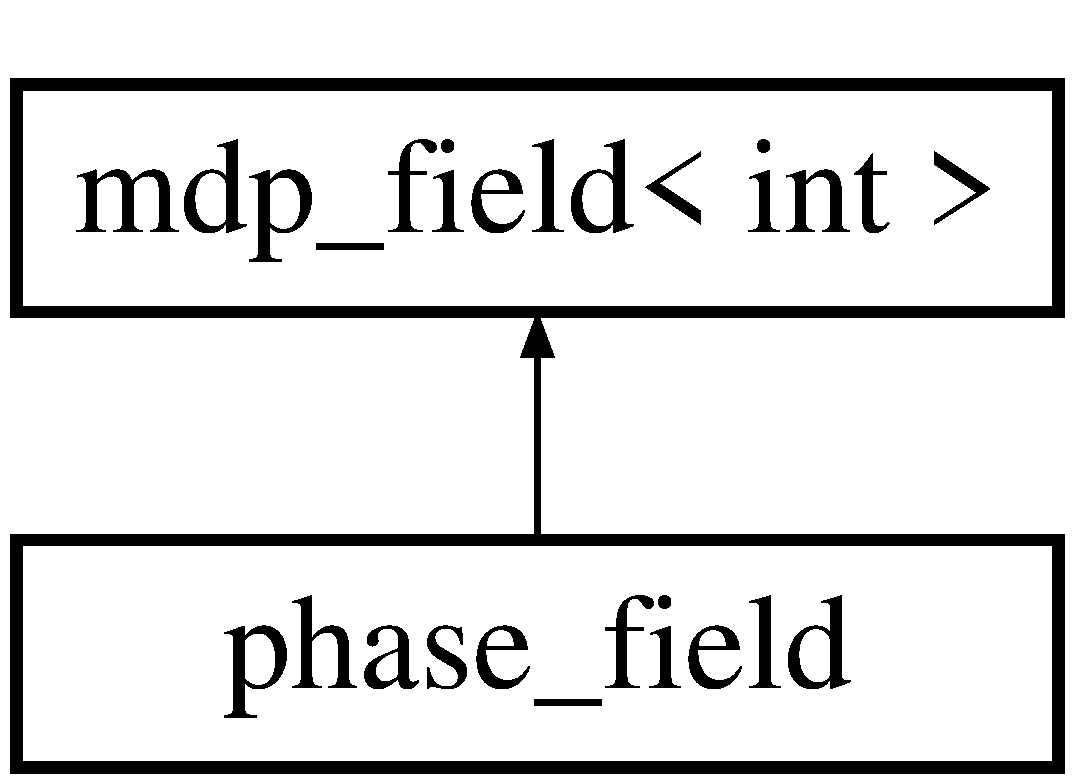
\includegraphics[height=2cm]{classphase__field}
\end{center}
\end{figure}
\subsection*{Public Member Functions}
\begin{DoxyCompactItemize}
\item 
\hyperlink{classphase__field_ad57c78000dce7ec4316117b5a1451c1f}{phase\_\-field} (\hyperlink{classmdp__lattice}{mdp\_\-lattice} \&a)
\item 
int \hyperlink{classphase__field_aa4837d1dbdef924550e2c473b8cb7cd0}{component} (site x, site y)
\item 
void \hyperlink{classphase__field_a00ef00d8126c1ce8d68b53d67d217902}{compute} (\hyperlink{classmdp__matrix}{mdp\_\-matrix} GAMMA, \hyperlink{classmdp__matrix}{mdp\_\-matrix} ZETA)
\end{DoxyCompactItemize}


\subsection{Constructor \& Destructor Documentation}
\hypertarget{classphase__field_ad57c78000dce7ec4316117b5a1451c1f}{
\index{phase\_\-field@{phase\_\-field}!phase\_\-field@{phase\_\-field}}
\index{phase\_\-field@{phase\_\-field}!phase_field@{phase\_\-field}}
\subsubsection[{phase\_\-field}]{\setlength{\rightskip}{0pt plus 5cm}phase\_\-field::phase\_\-field ({\bf mdp\_\-lattice} \& {\em a})\hspace{0.3cm}{\ttfamily  \mbox{[}inline\mbox{]}}}}
\label{classphase__field_ad57c78000dce7ec4316117b5a1451c1f}


\subsection{Member Function Documentation}
\hypertarget{classphase__field_aa4837d1dbdef924550e2c473b8cb7cd0}{
\index{phase\_\-field@{phase\_\-field}!component@{component}}
\index{component@{component}!phase_field@{phase\_\-field}}
\subsubsection[{component}]{\setlength{\rightskip}{0pt plus 5cm}int phase\_\-field::component (site {\em x}, \/  site {\em y})\hspace{0.3cm}{\ttfamily  \mbox{[}inline\mbox{]}}}}
\label{classphase__field_aa4837d1dbdef924550e2c473b8cb7cd0}
\hypertarget{classphase__field_a00ef00d8126c1ce8d68b53d67d217902}{
\index{phase\_\-field@{phase\_\-field}!compute@{compute}}
\index{compute@{compute}!phase_field@{phase\_\-field}}
\subsubsection[{compute}]{\setlength{\rightskip}{0pt plus 5cm}void phase\_\-field::compute ({\bf mdp\_\-matrix} {\em GAMMA}, \/  {\bf mdp\_\-matrix} {\em ZETA})\hspace{0.3cm}{\ttfamily  \mbox{[}inline\mbox{]}}}}
\label{classphase__field_a00ef00d8126c1ce8d68b53d67d217902}


The documentation for this class was generated from the following file:\begin{DoxyCompactItemize}
\item 
/Users/mdipierro/fermiqcd/development/Libraries/\hyperlink{fermiqcd__staggered__mesons_8h}{fermiqcd\_\-staggered\_\-mesons.h}\end{DoxyCompactItemize}

\hypertarget{classsdwf__field}{
\section{sdwf\_\-field Class Reference}
\label{classsdwf__field}\index{sdwf\_\-field@{sdwf\_\-field}}
}


field for domain wall staggered fermions  


{\ttfamily \#include $<$fermiqcd\_\-sdwf\_\-field.h$>$}Inheritance diagram for sdwf\_\-field::\begin{figure}[H]
\begin{center}
\leavevmode
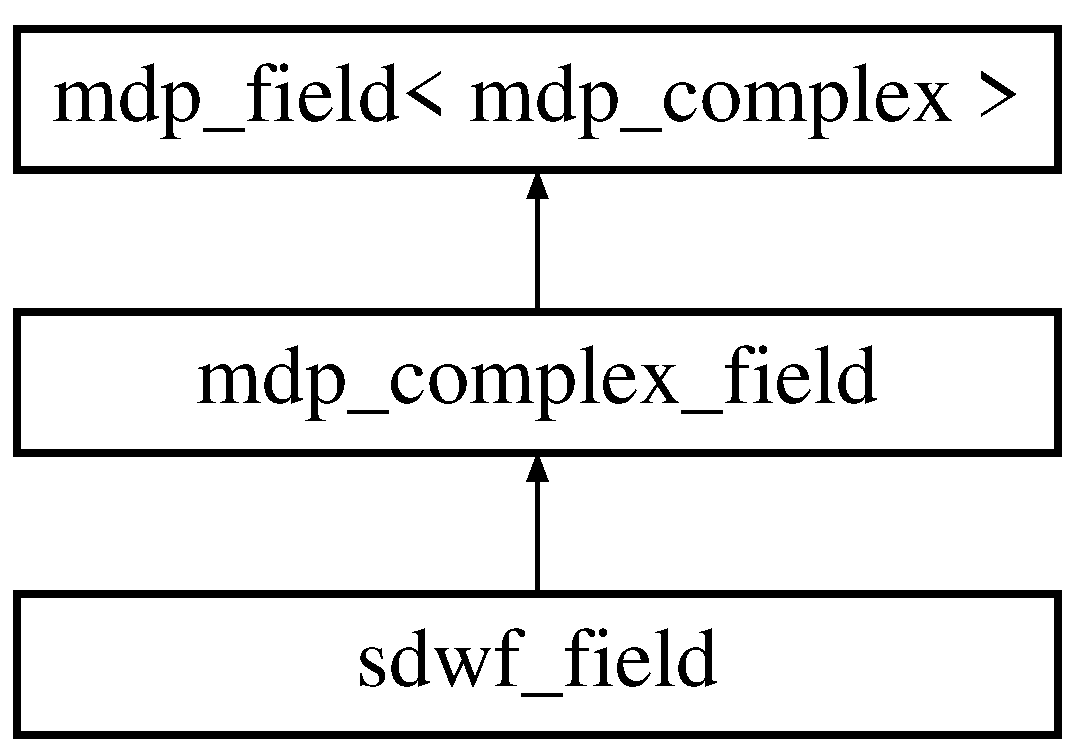
\includegraphics[height=3cm]{classsdwf__field}
\end{center}
\end{figure}
\subsection*{Public Member Functions}
\begin{DoxyCompactItemize}
\item 
\hyperlink{classsdwf__field_a904cdf6c1f542aa5d4873b5c049a0de5}{sdwf\_\-field} (\hyperlink{classmdp__lattice}{mdp\_\-lattice} \&a, int L5\_\-, int nc\_\-, int nspin\_\-=4)
\item 
\hyperlink{classsdwf__field_af1438250ba08d632c4906ef99ad907ea}{sdwf\_\-field} (\hyperlink{classsdwf__field}{sdwf\_\-field} \&chi)
\item 
\hyperlink{classmdp__matrix}{mdp\_\-matrix} \hyperlink{classsdwf__field_a18764312ba3bb72577b2e29429854024}{operator()} (site x, int x5)
\item 
\hyperlink{classmdp__complex}{mdp\_\-complex} \& \hyperlink{classsdwf__field_a1cd68e8911b77c60ecd6a1cd245ec047}{operator()} (site x, int x5, int i)
\item 
const \hyperlink{classmdp__complex}{mdp\_\-complex} \& \hyperlink{classsdwf__field_a205e5f728691c6bfe350335a477e42c7}{operator()} (site x, int x5, int i) const 
\item 
void \hyperlink{classsdwf__field_ac9bbccf6442b9f1a1a07b18fd2fe442c}{operator=} (\hyperlink{classmdp__complex}{mdp\_\-complex} a)
\item 
\hyperlink{mdp__global__vars_8h_a049e4c1d4e74d644878a42f9909463e4}{mdp\_\-real} \hyperlink{classsdwf__field_aa834c736322bef716cd0e31a391623d3}{component} (site x, int mu)
\item 
\hyperlink{mdp__global__vars_8h_a049e4c1d4e74d644878a42f9909463e4}{mdp\_\-real} \hyperlink{classsdwf__field_ae50c1b9db65cd8056ed9286bde99e791}{eta} (site x, int mu)
\item 
\hyperlink{mdp__global__vars_8h_a049e4c1d4e74d644878a42f9909463e4}{mdp\_\-real} \hyperlink{classsdwf__field_a3cc6aef9972ab5cceab9646578857db0}{eps} (site x)
\item 
\hyperlink{mdp__global__vars_8h_a049e4c1d4e74d644878a42f9909463e4}{mdp\_\-real} \hyperlink{classsdwf__field_a7227345aef0414528513479dad854568}{type} (site x)
\item 
site \hyperlink{classsdwf__field_a5cff8766c1891c6240c97d17c6bb63b9}{chiral\_\-shift} (site x)
\item 
\hyperlink{mdp__global__vars_8h_a049e4c1d4e74d644878a42f9909463e4}{mdp\_\-real} \hyperlink{classsdwf__field_a29fce204e377b7a190455e4faf0a2a0c}{chiral\_\-phase} (site x)
\item 
\hyperlink{mdp__global__vars_8h_a049e4c1d4e74d644878a42f9909463e4}{mdp\_\-real} \hyperlink{classsdwf__field_a67fe2a75323e3dcfce3675cce0bbb312}{chiral\_\-phase2} (site x)
\end{DoxyCompactItemize}
\subsection*{Public Attributes}
\begin{DoxyCompactItemize}
\item 
int \hyperlink{classsdwf__field_a957d5e1caa928243ec4224cf1e2861f1}{nc}
\item 
int \hyperlink{classsdwf__field_a5a861ccb2b42b333b5d67e3b501e8533}{ndim}
\item 
int \hyperlink{classsdwf__field_a6269e653489fd6ee9340da498187b132}{nspin}
\item 
int \hyperlink{classsdwf__field_a19bd0e3027574c1204f8aa3f6635d1df}{L5}
\end{DoxyCompactItemize}


\subsection{Detailed Description}
field for domain wall staggered fermions 

\subsection{Constructor \& Destructor Documentation}
\hypertarget{classsdwf__field_a904cdf6c1f542aa5d4873b5c049a0de5}{
\index{sdwf\_\-field@{sdwf\_\-field}!sdwf\_\-field@{sdwf\_\-field}}
\index{sdwf\_\-field@{sdwf\_\-field}!sdwf_field@{sdwf\_\-field}}
\subsubsection[{sdwf\_\-field}]{\setlength{\rightskip}{0pt plus 5cm}sdwf\_\-field::sdwf\_\-field ({\bf mdp\_\-lattice} \& {\em a}, \/  int {\em L5\_\-}, \/  int {\em nc\_\-}, \/  int {\em nspin\_\-} = {\ttfamily 4})\hspace{0.3cm}{\ttfamily  \mbox{[}inline\mbox{]}}}}
\label{classsdwf__field_a904cdf6c1f542aa5d4873b5c049a0de5}
\hypertarget{classsdwf__field_af1438250ba08d632c4906ef99ad907ea}{
\index{sdwf\_\-field@{sdwf\_\-field}!sdwf\_\-field@{sdwf\_\-field}}
\index{sdwf\_\-field@{sdwf\_\-field}!sdwf_field@{sdwf\_\-field}}
\subsubsection[{sdwf\_\-field}]{\setlength{\rightskip}{0pt plus 5cm}sdwf\_\-field::sdwf\_\-field ({\bf sdwf\_\-field} \& {\em chi})\hspace{0.3cm}{\ttfamily  \mbox{[}inline\mbox{]}}}}
\label{classsdwf__field_af1438250ba08d632c4906ef99ad907ea}


\subsection{Member Function Documentation}
\hypertarget{classsdwf__field_a29fce204e377b7a190455e4faf0a2a0c}{
\index{sdwf\_\-field@{sdwf\_\-field}!chiral\_\-phase@{chiral\_\-phase}}
\index{chiral\_\-phase@{chiral\_\-phase}!sdwf_field@{sdwf\_\-field}}
\subsubsection[{chiral\_\-phase}]{\setlength{\rightskip}{0pt plus 5cm}{\bf mdp\_\-real} sdwf\_\-field::chiral\_\-phase (site {\em x})\hspace{0.3cm}{\ttfamily  \mbox{[}inline\mbox{]}}}}
\label{classsdwf__field_a29fce204e377b7a190455e4faf0a2a0c}
\hypertarget{classsdwf__field_a67fe2a75323e3dcfce3675cce0bbb312}{
\index{sdwf\_\-field@{sdwf\_\-field}!chiral\_\-phase2@{chiral\_\-phase2}}
\index{chiral\_\-phase2@{chiral\_\-phase2}!sdwf_field@{sdwf\_\-field}}
\subsubsection[{chiral\_\-phase2}]{\setlength{\rightskip}{0pt plus 5cm}{\bf mdp\_\-real} sdwf\_\-field::chiral\_\-phase2 (site {\em x})\hspace{0.3cm}{\ttfamily  \mbox{[}inline\mbox{]}}}}
\label{classsdwf__field_a67fe2a75323e3dcfce3675cce0bbb312}
\hypertarget{classsdwf__field_a5cff8766c1891c6240c97d17c6bb63b9}{
\index{sdwf\_\-field@{sdwf\_\-field}!chiral\_\-shift@{chiral\_\-shift}}
\index{chiral\_\-shift@{chiral\_\-shift}!sdwf_field@{sdwf\_\-field}}
\subsubsection[{chiral\_\-shift}]{\setlength{\rightskip}{0pt plus 5cm}site sdwf\_\-field::chiral\_\-shift (site {\em x})\hspace{0.3cm}{\ttfamily  \mbox{[}inline\mbox{]}}}}
\label{classsdwf__field_a5cff8766c1891c6240c97d17c6bb63b9}
\hypertarget{classsdwf__field_aa834c736322bef716cd0e31a391623d3}{
\index{sdwf\_\-field@{sdwf\_\-field}!component@{component}}
\index{component@{component}!sdwf_field@{sdwf\_\-field}}
\subsubsection[{component}]{\setlength{\rightskip}{0pt plus 5cm}{\bf mdp\_\-real} sdwf\_\-field::component (site {\em x}, \/  int {\em mu})\hspace{0.3cm}{\ttfamily  \mbox{[}inline\mbox{]}}}}
\label{classsdwf__field_aa834c736322bef716cd0e31a391623d3}
\hypertarget{classsdwf__field_a3cc6aef9972ab5cceab9646578857db0}{
\index{sdwf\_\-field@{sdwf\_\-field}!eps@{eps}}
\index{eps@{eps}!sdwf_field@{sdwf\_\-field}}
\subsubsection[{eps}]{\setlength{\rightskip}{0pt plus 5cm}{\bf mdp\_\-real} sdwf\_\-field::eps (site {\em x})\hspace{0.3cm}{\ttfamily  \mbox{[}inline\mbox{]}}}}
\label{classsdwf__field_a3cc6aef9972ab5cceab9646578857db0}
\hypertarget{classsdwf__field_ae50c1b9db65cd8056ed9286bde99e791}{
\index{sdwf\_\-field@{sdwf\_\-field}!eta@{eta}}
\index{eta@{eta}!sdwf_field@{sdwf\_\-field}}
\subsubsection[{eta}]{\setlength{\rightskip}{0pt plus 5cm}{\bf mdp\_\-real} sdwf\_\-field::eta (site {\em x}, \/  int {\em mu})\hspace{0.3cm}{\ttfamily  \mbox{[}inline\mbox{]}}}}
\label{classsdwf__field_ae50c1b9db65cd8056ed9286bde99e791}
\hypertarget{classsdwf__field_a205e5f728691c6bfe350335a477e42c7}{
\index{sdwf\_\-field@{sdwf\_\-field}!operator()@{operator()}}
\index{operator()@{operator()}!sdwf_field@{sdwf\_\-field}}
\subsubsection[{operator()}]{\setlength{\rightskip}{0pt plus 5cm}const {\bf mdp\_\-complex}\& sdwf\_\-field::operator() (site {\em x}, \/  int {\em x5}, \/  int {\em i}) const\hspace{0.3cm}{\ttfamily  \mbox{[}inline\mbox{]}}}}
\label{classsdwf__field_a205e5f728691c6bfe350335a477e42c7}
\hypertarget{classsdwf__field_a1cd68e8911b77c60ecd6a1cd245ec047}{
\index{sdwf\_\-field@{sdwf\_\-field}!operator()@{operator()}}
\index{operator()@{operator()}!sdwf_field@{sdwf\_\-field}}
\subsubsection[{operator()}]{\setlength{\rightskip}{0pt plus 5cm}{\bf mdp\_\-complex}\& sdwf\_\-field::operator() (site {\em x}, \/  int {\em x5}, \/  int {\em i})\hspace{0.3cm}{\ttfamily  \mbox{[}inline\mbox{]}}}}
\label{classsdwf__field_a1cd68e8911b77c60ecd6a1cd245ec047}
\hypertarget{classsdwf__field_a18764312ba3bb72577b2e29429854024}{
\index{sdwf\_\-field@{sdwf\_\-field}!operator()@{operator()}}
\index{operator()@{operator()}!sdwf_field@{sdwf\_\-field}}
\subsubsection[{operator()}]{\setlength{\rightskip}{0pt plus 5cm}{\bf mdp\_\-matrix} sdwf\_\-field::operator() (site {\em x}, \/  int {\em x5})\hspace{0.3cm}{\ttfamily  \mbox{[}inline\mbox{]}}}}
\label{classsdwf__field_a18764312ba3bb72577b2e29429854024}
\hypertarget{classsdwf__field_ac9bbccf6442b9f1a1a07b18fd2fe442c}{
\index{sdwf\_\-field@{sdwf\_\-field}!operator=@{operator=}}
\index{operator=@{operator=}!sdwf_field@{sdwf\_\-field}}
\subsubsection[{operator=}]{\setlength{\rightskip}{0pt plus 5cm}void sdwf\_\-field::operator= ({\bf mdp\_\-complex} {\em a})\hspace{0.3cm}{\ttfamily  \mbox{[}inline\mbox{]}}}}
\label{classsdwf__field_ac9bbccf6442b9f1a1a07b18fd2fe442c}


Reimplemented from \hyperlink{classmdp__field_a24364bce6444668661a0688632af87ec}{mdp\_\-field$<$ mdp\_\-complex $>$}.\hypertarget{classsdwf__field_a7227345aef0414528513479dad854568}{
\index{sdwf\_\-field@{sdwf\_\-field}!type@{type}}
\index{type@{type}!sdwf_field@{sdwf\_\-field}}
\subsubsection[{type}]{\setlength{\rightskip}{0pt plus 5cm}{\bf mdp\_\-real} sdwf\_\-field::type (site {\em x})\hspace{0.3cm}{\ttfamily  \mbox{[}inline\mbox{]}}}}
\label{classsdwf__field_a7227345aef0414528513479dad854568}


\subsection{Member Data Documentation}
\hypertarget{classsdwf__field_a19bd0e3027574c1204f8aa3f6635d1df}{
\index{sdwf\_\-field@{sdwf\_\-field}!L5@{L5}}
\index{L5@{L5}!sdwf_field@{sdwf\_\-field}}
\subsubsection[{L5}]{\setlength{\rightskip}{0pt plus 5cm}int {\bf sdwf\_\-field::L5}}}
\label{classsdwf__field_a19bd0e3027574c1204f8aa3f6635d1df}
\hypertarget{classsdwf__field_a957d5e1caa928243ec4224cf1e2861f1}{
\index{sdwf\_\-field@{sdwf\_\-field}!nc@{nc}}
\index{nc@{nc}!sdwf_field@{sdwf\_\-field}}
\subsubsection[{nc}]{\setlength{\rightskip}{0pt plus 5cm}int {\bf sdwf\_\-field::nc}}}
\label{classsdwf__field_a957d5e1caa928243ec4224cf1e2861f1}
\hypertarget{classsdwf__field_a5a861ccb2b42b333b5d67e3b501e8533}{
\index{sdwf\_\-field@{sdwf\_\-field}!ndim@{ndim}}
\index{ndim@{ndim}!sdwf_field@{sdwf\_\-field}}
\subsubsection[{ndim}]{\setlength{\rightskip}{0pt plus 5cm}int {\bf sdwf\_\-field::ndim}}}
\label{classsdwf__field_a5a861ccb2b42b333b5d67e3b501e8533}
\hypertarget{classsdwf__field_a6269e653489fd6ee9340da498187b132}{
\index{sdwf\_\-field@{sdwf\_\-field}!nspin@{nspin}}
\index{nspin@{nspin}!sdwf_field@{sdwf\_\-field}}
\subsubsection[{nspin}]{\setlength{\rightskip}{0pt plus 5cm}int {\bf sdwf\_\-field::nspin}}}
\label{classsdwf__field_a6269e653489fd6ee9340da498187b132}


The documentation for this class was generated from the following file:\begin{DoxyCompactItemize}
\item 
/Users/mdipierro/fermiqcd/development/Libraries/\hyperlink{fermiqcd__sdwf__field_8h}{fermiqcd\_\-sdwf\_\-field.h}\end{DoxyCompactItemize}

\hypertarget{class_s_d_w_f_action_slow}{
\section{SDWFActionSlow Class Reference}
\label{class_s_d_w_f_action_slow}\index{SDWFActionSlow@{SDWFActionSlow}}
}
domain wall staggered (WORK IN PROGRESS)  


{\tt \#include $<$fermiqcd\_\-sdwf\_\-actions.h$>$}



\subsection{Detailed Description}
domain wall staggered (WORK IN PROGRESS) 

The documentation for this class was generated from the following file:\begin{CompactItemize}
\item 
/Users/mdipierro/Desktop/SciDac/development/Libraries/\hyperlink{fermiqcd__sdwf__actions_8h}{fermiqcd\_\-sdwf\_\-actions.h}\end{CompactItemize}

\hypertarget{classstaggered__field}{
\section{staggered\_\-field Class Reference}
\label{classstaggered__field}\index{staggered\_\-field@{staggered\_\-field}}
}


staggered fermionic field  


{\ttfamily \#include $<$fermiqcd\_\-staggered\_\-field.h$>$}Inheritance diagram for staggered\_\-field::\begin{figure}[H]
\begin{center}
\leavevmode
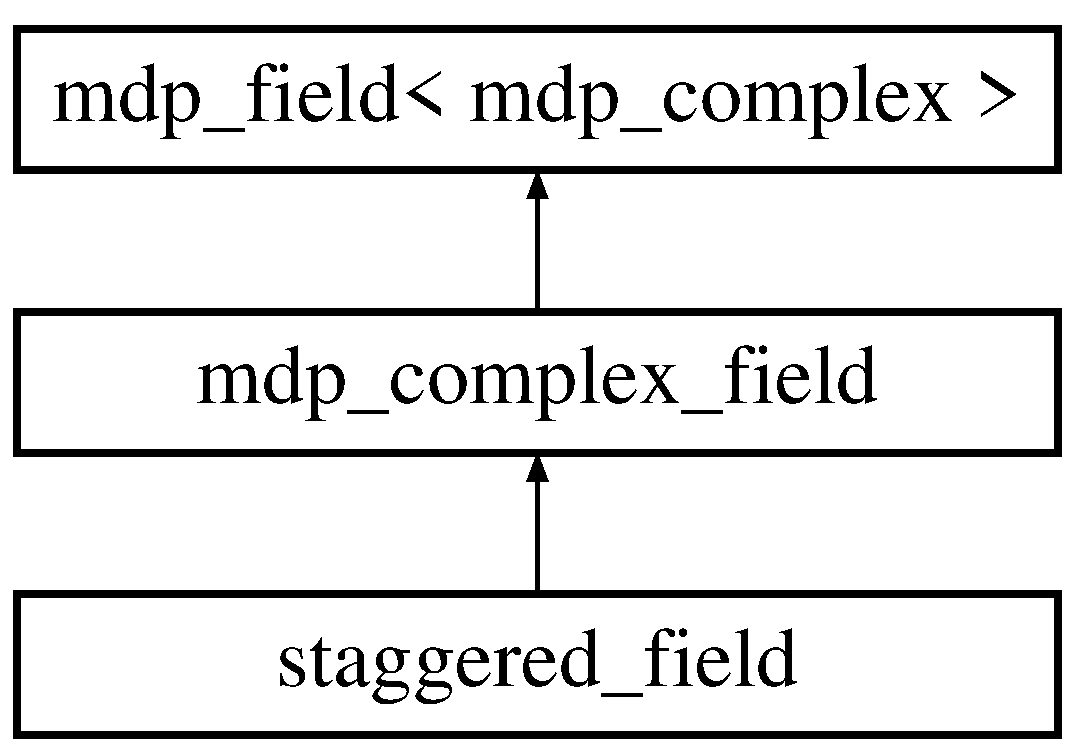
\includegraphics[height=3cm]{classstaggered__field}
\end{center}
\end{figure}
\subsection*{Public Member Functions}
\begin{DoxyCompactItemize}
\item 
\hyperlink{classstaggered__field_acc7d5a171caf8bda9d0a904c6672432d}{staggered\_\-field} (\hyperlink{classmdp__lattice}{mdp\_\-lattice} \&a, int nc\_\-, int nspin\_\-=4)
\item 
\hyperlink{classstaggered__field_a22b5b7f7d050f6356451df02356f181d}{staggered\_\-field} (const \hyperlink{classstaggered__field}{staggered\_\-field} \&chi)
\item 
void \hyperlink{classstaggered__field_a5320371c9d4b87255c578e5b41684e48}{operator=} (const \hyperlink{classstaggered__field}{staggered\_\-field} \&chi)
\item 
\hyperlink{classmdp__matrix}{mdp\_\-matrix} \hyperlink{classstaggered__field_aa881451872889aa0b6c716c01f3fabb7}{operator()} (site x)
\item 
\hyperlink{classmdp__complex}{mdp\_\-complex} \& \hyperlink{classstaggered__field_a32b4553845d0b7f92f99f07e0fbeb64a}{operator()} (site x, int i)
\item 
const \hyperlink{classmdp__complex}{mdp\_\-complex} \& \hyperlink{classstaggered__field_a8cee97da0e262753ab059ef553597a01}{operator()} (site x, int i) const 
\item 
void \hyperlink{classstaggered__field_ac3fee1898eaa4198744c5bc0cc969e2e}{operator=} (\hyperlink{classmdp__complex}{mdp\_\-complex} a)
\item 
\hyperlink{mdp__global__vars_8h_a049e4c1d4e74d644878a42f9909463e4}{mdp\_\-real} \hyperlink{classstaggered__field_a613e227e2cc092c103ce431000fd4b53}{component} (site x, int mu)
\item 
\hyperlink{mdp__global__vars_8h_a049e4c1d4e74d644878a42f9909463e4}{mdp\_\-real} \hyperlink{classstaggered__field_a2f865e7dbd982109e584d26687f5340d}{eta} (site x, int mu)
\item 
\hyperlink{mdp__global__vars_8h_a049e4c1d4e74d644878a42f9909463e4}{mdp\_\-real} \hyperlink{classstaggered__field_ae89b67366b3566c3c8a89d3303dc1d62}{eps} (site x)
\item 
\hyperlink{mdp__global__vars_8h_a049e4c1d4e74d644878a42f9909463e4}{mdp\_\-real} \hyperlink{classstaggered__field_a5e53f3e9e5c268dde3e3f2eb9e64befa}{type} (site x)
\end{DoxyCompactItemize}
\subsection*{Public Attributes}
\begin{DoxyCompactItemize}
\item 
int \hyperlink{classstaggered__field_a4ac408eebebb6b76ac209479df87459a}{nc}
\item 
int \hyperlink{classstaggered__field_a52eed99381c8e8649c6e79ec0fe7a4b8}{ndim}
\item 
int \hyperlink{classstaggered__field_aac06f4fadf069a57cda02bec2ecd8bda}{nspin}
\end{DoxyCompactItemize}


\subsection{Detailed Description}
staggered fermionic field Example: \begin{DoxyVerb}
/// staggered_field psi(lattice,nc);
/// mdp_site x(lattice);
/// forallsites(x)
///   for(int i=0; i<nc; i++)
///     psi(x,i)=0.0+0.0*I;
/// \end{DoxyVerb}
 

\subsection{Constructor \& Destructor Documentation}
\hypertarget{classstaggered__field_acc7d5a171caf8bda9d0a904c6672432d}{
\index{staggered\_\-field@{staggered\_\-field}!staggered\_\-field@{staggered\_\-field}}
\index{staggered\_\-field@{staggered\_\-field}!staggered_field@{staggered\_\-field}}
\subsubsection[{staggered\_\-field}]{\setlength{\rightskip}{0pt plus 5cm}staggered\_\-field::staggered\_\-field ({\bf mdp\_\-lattice} \& {\em a}, \/  int {\em nc\_\-}, \/  int {\em nspin\_\-} = {\ttfamily 4})\hspace{0.3cm}{\ttfamily  \mbox{[}inline\mbox{]}}}}
\label{classstaggered__field_acc7d5a171caf8bda9d0a904c6672432d}
\hypertarget{classstaggered__field_a22b5b7f7d050f6356451df02356f181d}{
\index{staggered\_\-field@{staggered\_\-field}!staggered\_\-field@{staggered\_\-field}}
\index{staggered\_\-field@{staggered\_\-field}!staggered_field@{staggered\_\-field}}
\subsubsection[{staggered\_\-field}]{\setlength{\rightskip}{0pt plus 5cm}staggered\_\-field::staggered\_\-field (const {\bf staggered\_\-field} \& {\em chi})\hspace{0.3cm}{\ttfamily  \mbox{[}inline\mbox{]}}}}
\label{classstaggered__field_a22b5b7f7d050f6356451df02356f181d}


\subsection{Member Function Documentation}
\hypertarget{classstaggered__field_a613e227e2cc092c103ce431000fd4b53}{
\index{staggered\_\-field@{staggered\_\-field}!component@{component}}
\index{component@{component}!staggered_field@{staggered\_\-field}}
\subsubsection[{component}]{\setlength{\rightskip}{0pt plus 5cm}{\bf mdp\_\-real} staggered\_\-field::component (site {\em x}, \/  int {\em mu})\hspace{0.3cm}{\ttfamily  \mbox{[}inline\mbox{]}}}}
\label{classstaggered__field_a613e227e2cc092c103ce431000fd4b53}
\hypertarget{classstaggered__field_ae89b67366b3566c3c8a89d3303dc1d62}{
\index{staggered\_\-field@{staggered\_\-field}!eps@{eps}}
\index{eps@{eps}!staggered_field@{staggered\_\-field}}
\subsubsection[{eps}]{\setlength{\rightskip}{0pt plus 5cm}{\bf mdp\_\-real} staggered\_\-field::eps (site {\em x})\hspace{0.3cm}{\ttfamily  \mbox{[}inline\mbox{]}}}}
\label{classstaggered__field_ae89b67366b3566c3c8a89d3303dc1d62}
\hypertarget{classstaggered__field_a2f865e7dbd982109e584d26687f5340d}{
\index{staggered\_\-field@{staggered\_\-field}!eta@{eta}}
\index{eta@{eta}!staggered_field@{staggered\_\-field}}
\subsubsection[{eta}]{\setlength{\rightskip}{0pt plus 5cm}{\bf mdp\_\-real} staggered\_\-field::eta (site {\em x}, \/  int {\em mu})\hspace{0.3cm}{\ttfamily  \mbox{[}inline\mbox{]}}}}
\label{classstaggered__field_a2f865e7dbd982109e584d26687f5340d}
\hypertarget{classstaggered__field_a8cee97da0e262753ab059ef553597a01}{
\index{staggered\_\-field@{staggered\_\-field}!operator()@{operator()}}
\index{operator()@{operator()}!staggered_field@{staggered\_\-field}}
\subsubsection[{operator()}]{\setlength{\rightskip}{0pt plus 5cm}const {\bf mdp\_\-complex}\& staggered\_\-field::operator() (site {\em x}, \/  int {\em i}) const\hspace{0.3cm}{\ttfamily  \mbox{[}inline\mbox{]}}}}
\label{classstaggered__field_a8cee97da0e262753ab059ef553597a01}
\hypertarget{classstaggered__field_a32b4553845d0b7f92f99f07e0fbeb64a}{
\index{staggered\_\-field@{staggered\_\-field}!operator()@{operator()}}
\index{operator()@{operator()}!staggered_field@{staggered\_\-field}}
\subsubsection[{operator()}]{\setlength{\rightskip}{0pt plus 5cm}{\bf mdp\_\-complex}\& staggered\_\-field::operator() (site {\em x}, \/  int {\em i})\hspace{0.3cm}{\ttfamily  \mbox{[}inline\mbox{]}}}}
\label{classstaggered__field_a32b4553845d0b7f92f99f07e0fbeb64a}
\hypertarget{classstaggered__field_aa881451872889aa0b6c716c01f3fabb7}{
\index{staggered\_\-field@{staggered\_\-field}!operator()@{operator()}}
\index{operator()@{operator()}!staggered_field@{staggered\_\-field}}
\subsubsection[{operator()}]{\setlength{\rightskip}{0pt plus 5cm}{\bf mdp\_\-matrix} staggered\_\-field::operator() (site {\em x})\hspace{0.3cm}{\ttfamily  \mbox{[}inline\mbox{]}}}}
\label{classstaggered__field_aa881451872889aa0b6c716c01f3fabb7}
\hypertarget{classstaggered__field_ac3fee1898eaa4198744c5bc0cc969e2e}{
\index{staggered\_\-field@{staggered\_\-field}!operator=@{operator=}}
\index{operator=@{operator=}!staggered_field@{staggered\_\-field}}
\subsubsection[{operator=}]{\setlength{\rightskip}{0pt plus 5cm}void staggered\_\-field::operator= ({\bf mdp\_\-complex} {\em a})\hspace{0.3cm}{\ttfamily  \mbox{[}inline\mbox{]}}}}
\label{classstaggered__field_ac3fee1898eaa4198744c5bc0cc969e2e}


Reimplemented from \hyperlink{classmdp__field_a24364bce6444668661a0688632af87ec}{mdp\_\-field$<$ mdp\_\-complex $>$}.\hypertarget{classstaggered__field_a5320371c9d4b87255c578e5b41684e48}{
\index{staggered\_\-field@{staggered\_\-field}!operator=@{operator=}}
\index{operator=@{operator=}!staggered_field@{staggered\_\-field}}
\subsubsection[{operator=}]{\setlength{\rightskip}{0pt plus 5cm}void staggered\_\-field::operator= (const {\bf staggered\_\-field} \& {\em chi})\hspace{0.3cm}{\ttfamily  \mbox{[}inline\mbox{]}}}}
\label{classstaggered__field_a5320371c9d4b87255c578e5b41684e48}


Reimplemented from \hyperlink{classmdp__complex__field_ad2b736ae31e3ee1f955c10f6ad40928f}{mdp\_\-complex\_\-field}.\hypertarget{classstaggered__field_a5e53f3e9e5c268dde3e3f2eb9e64befa}{
\index{staggered\_\-field@{staggered\_\-field}!type@{type}}
\index{type@{type}!staggered_field@{staggered\_\-field}}
\subsubsection[{type}]{\setlength{\rightskip}{0pt plus 5cm}{\bf mdp\_\-real} staggered\_\-field::type (site {\em x})\hspace{0.3cm}{\ttfamily  \mbox{[}inline\mbox{]}}}}
\label{classstaggered__field_a5e53f3e9e5c268dde3e3f2eb9e64befa}


\subsection{Member Data Documentation}
\hypertarget{classstaggered__field_a4ac408eebebb6b76ac209479df87459a}{
\index{staggered\_\-field@{staggered\_\-field}!nc@{nc}}
\index{nc@{nc}!staggered_field@{staggered\_\-field}}
\subsubsection[{nc}]{\setlength{\rightskip}{0pt plus 5cm}int {\bf staggered\_\-field::nc}}}
\label{classstaggered__field_a4ac408eebebb6b76ac209479df87459a}
\hypertarget{classstaggered__field_a52eed99381c8e8649c6e79ec0fe7a4b8}{
\index{staggered\_\-field@{staggered\_\-field}!ndim@{ndim}}
\index{ndim@{ndim}!staggered_field@{staggered\_\-field}}
\subsubsection[{ndim}]{\setlength{\rightskip}{0pt plus 5cm}int {\bf staggered\_\-field::ndim}}}
\label{classstaggered__field_a52eed99381c8e8649c6e79ec0fe7a4b8}
\hypertarget{classstaggered__field_aac06f4fadf069a57cda02bec2ecd8bda}{
\index{staggered\_\-field@{staggered\_\-field}!nspin@{nspin}}
\index{nspin@{nspin}!staggered_field@{staggered\_\-field}}
\subsubsection[{nspin}]{\setlength{\rightskip}{0pt plus 5cm}int {\bf staggered\_\-field::nspin}}}
\label{classstaggered__field_aac06f4fadf069a57cda02bec2ecd8bda}


The documentation for this class was generated from the following file:\begin{DoxyCompactItemize}
\item 
/Users/mdipierro/fermiqcd/development/Libraries/\hyperlink{fermiqcd__staggered__field_8h}{fermiqcd\_\-staggered\_\-field.h}\end{DoxyCompactItemize}

\hypertarget{classstaggered__propagator}{
\section{staggered\_\-propagator Class Reference}
\label{classstaggered__propagator}\index{staggered\_\-propagator@{staggered\_\-propagator}}
}


staggared quark propagator  


{\ttfamily \#include $<$fermiqcd\_\-staggered\_\-propagator.h$>$}Inheritance diagram for staggered\_\-propagator::\begin{figure}[H]
\begin{center}
\leavevmode
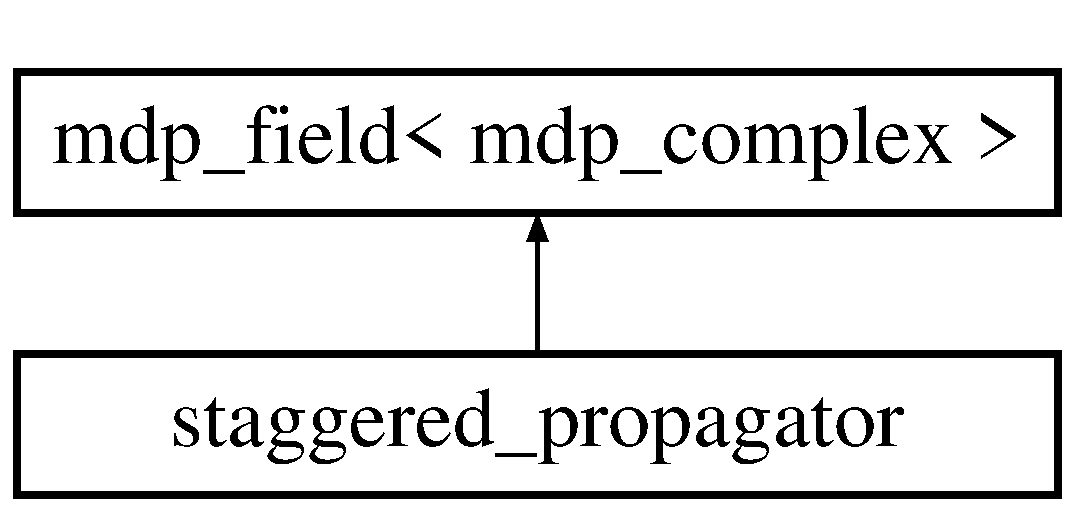
\includegraphics[height=2cm]{classstaggered__propagator}
\end{center}
\end{figure}
\subsection*{Public Member Functions}
\begin{DoxyCompactItemize}
\item 
\hyperlink{classstaggered__propagator_ad2abd9534d09d4f0af54a53ed4e092c6}{staggered\_\-propagator} (\hyperlink{classmdp__lattice}{mdp\_\-lattice} \&mylattice, int nc\_\-)
\item 
\hyperlink{classmdp__matrix}{mdp\_\-matrix} \hyperlink{classstaggered__propagator_ae5c5d6720631c30938b09de4d3331e7f}{operator()} (site x, int a)
\item 
\hyperlink{classmdp__complex}{mdp\_\-complex} \& \hyperlink{classstaggered__propagator_aed9bbdd906e6e68f806a895c5e1bd2d8}{operator()} (site x, int a, int i, int j)
\end{DoxyCompactItemize}
\subsection*{Public Attributes}
\begin{DoxyCompactItemize}
\item 
int \hyperlink{classstaggered__propagator_a1f2816b7b6b4f9b6779224fcdd0d6aff}{nc}
\end{DoxyCompactItemize}
\subsection*{Friends}
\begin{DoxyCompactItemize}
\item 
void \hyperlink{classstaggered__propagator_a7849b2db88d889afda04b4ee01476b64}{generate} (\hyperlink{classstaggered__propagator}{staggered\_\-propagator} \&S, \hyperlink{classgauge__field}{gauge\_\-field} \&U, \hyperlink{classcoefficients}{coefficients} \&coeff, \hyperlink{mdp__global__vars_8h_a049e4c1d4e74d644878a42f9909463e4}{mdp\_\-real} absolute\_\-precision=\hyperlink{fermiqcd__default__parameters_8h_ab11c95dc923c6bfd349bd67af277d59d}{fermi\_\-inversion\_\-precision}, \hyperlink{mdp__global__vars_8h_a049e4c1d4e74d644878a42f9909463e4}{mdp\_\-real} relative\_\-precision=0, int max\_\-steps=2000, void($\ast$smf)(\hyperlink{classstaggered__field}{staggered\_\-field} \&, \hyperlink{classgauge__field}{gauge\_\-field} \&)=0, int comp=0)
\end{DoxyCompactItemize}


\subsection{Detailed Description}
staggared quark propagator On a (2n) dimensional lattice this makes 3$\ast$(2$^\wedge$n) sources at the vertices of the hypercube at the origin of the lattice and inverts the Staggered/Asqtad action on them.

Example: \begin{DoxyVerb}
/// mdp_gauge U(lattice,nc);
/// staggered_propagator S(lattice,nc);
/// mdp_site x(lattice);
/// mdp_site y(lattice);
/// coefficients coeff;
/// coeff["mass"]=1.0;
/// generate(S,U,coeff);
/// for(int i=0; i<(int) pow(2,lattice.ndim); i++) {
///    x=binary2versor(a);
///    cout << "source at:" << x << "\nprop:\n"; 
///    forallsites(y) cout << S(x,a) << endl;
/// }
/// \end{DoxyVerb}
 

\subsection{Constructor \& Destructor Documentation}
\hypertarget{classstaggered__propagator_ad2abd9534d09d4f0af54a53ed4e092c6}{
\index{staggered\_\-propagator@{staggered\_\-propagator}!staggered\_\-propagator@{staggered\_\-propagator}}
\index{staggered\_\-propagator@{staggered\_\-propagator}!staggered_propagator@{staggered\_\-propagator}}
\subsubsection[{staggered\_\-propagator}]{\setlength{\rightskip}{0pt plus 5cm}staggered\_\-propagator::staggered\_\-propagator ({\bf mdp\_\-lattice} \& {\em mylattice}, \/  int {\em nc\_\-})\hspace{0.3cm}{\ttfamily  \mbox{[}inline\mbox{]}}}}
\label{classstaggered__propagator_ad2abd9534d09d4f0af54a53ed4e092c6}


\subsection{Member Function Documentation}
\hypertarget{classstaggered__propagator_aed9bbdd906e6e68f806a895c5e1bd2d8}{
\index{staggered\_\-propagator@{staggered\_\-propagator}!operator()@{operator()}}
\index{operator()@{operator()}!staggered_propagator@{staggered\_\-propagator}}
\subsubsection[{operator()}]{\setlength{\rightskip}{0pt plus 5cm}{\bf mdp\_\-complex}\& staggered\_\-propagator::operator() (site {\em x}, \/  int {\em a}, \/  int {\em i}, \/  int {\em j})\hspace{0.3cm}{\ttfamily  \mbox{[}inline\mbox{]}}}}
\label{classstaggered__propagator_aed9bbdd906e6e68f806a895c5e1bd2d8}
\hypertarget{classstaggered__propagator_ae5c5d6720631c30938b09de4d3331e7f}{
\index{staggered\_\-propagator@{staggered\_\-propagator}!operator()@{operator()}}
\index{operator()@{operator()}!staggered_propagator@{staggered\_\-propagator}}
\subsubsection[{operator()}]{\setlength{\rightskip}{0pt plus 5cm}{\bf mdp\_\-matrix} staggered\_\-propagator::operator() (site {\em x}, \/  int {\em a})\hspace{0.3cm}{\ttfamily  \mbox{[}inline\mbox{]}}}}
\label{classstaggered__propagator_ae5c5d6720631c30938b09de4d3331e7f}


\subsection{Friends And Related Function Documentation}
\hypertarget{classstaggered__propagator_a7849b2db88d889afda04b4ee01476b64}{
\index{staggered\_\-propagator@{staggered\_\-propagator}!generate@{generate}}
\index{generate@{generate}!staggered_propagator@{staggered\_\-propagator}}
\subsubsection[{generate}]{\setlength{\rightskip}{0pt plus 5cm}void generate ({\bf staggered\_\-propagator} \& {\em S}, \/  {\bf gauge\_\-field} \& {\em U}, \/  {\bf coefficients} \& {\em coeff}, \/  {\bf mdp\_\-real} {\em absolute\_\-precision} = {\ttfamily {\bf fermi\_\-inversion\_\-precision}}, \/  {\bf mdp\_\-real} {\em relative\_\-precision} = {\ttfamily 0}, \/  int {\em max\_\-steps} = {\ttfamily 2000}, \/  void($\ast$)({\bf staggered\_\-field} \&, {\bf gauge\_\-field} \&) {\em smf} = {\ttfamily 0}, \/  int {\em comp} = {\ttfamily 0})\hspace{0.3cm}{\ttfamily  \mbox{[}friend\mbox{]}}}}
\label{classstaggered__propagator_a7849b2db88d889afda04b4ee01476b64}


\subsection{Member Data Documentation}
\hypertarget{classstaggered__propagator_a1f2816b7b6b4f9b6779224fcdd0d6aff}{
\index{staggered\_\-propagator@{staggered\_\-propagator}!nc@{nc}}
\index{nc@{nc}!staggered_propagator@{staggered\_\-propagator}}
\subsubsection[{nc}]{\setlength{\rightskip}{0pt plus 5cm}int {\bf staggered\_\-propagator::nc}}}
\label{classstaggered__propagator_a1f2816b7b6b4f9b6779224fcdd0d6aff}


The documentation for this class was generated from the following file:\begin{DoxyCompactItemize}
\item 
/Users/mdipierro/fermiqcd/development/Libraries/\hyperlink{fermiqcd__staggered__propagator_8h}{fermiqcd\_\-staggered\_\-propagator.h}\end{DoxyCompactItemize}

\hypertarget{class_staggered_asqtad_action_fast}{
\section{StaggeredAsqtadActionFast Class Reference}
\label{class_staggered_asqtad_action_fast}\index{StaggeredAsqtadActionFast@{StaggeredAsqtadActionFast}}
}
Staggered/Asqtad action.  


{\tt \#include $<$fermiqcd\_\-staggered\_\-actions.h$>$}



\subsection{Detailed Description}
Staggered/Asqtad action. 

Example: 

\footnotesize\begin{verbatim}
/// gauge_field U(lattice,nc);
/// staggered_field psi(lattice,nc);
/// staggered_field chi(lattice,nc);
/// coefficients coeff;
/// coeff["mass"]=2.0;
/// default_staggered_action=StaggeredAsqtadActionFast::mul_Q;
/// mul_Q(chi,psi,U,coeff);
/// \end{verbatim}
\normalsize
 

The documentation for this class was generated from the following file:\begin{CompactItemize}
\item 
/Users/mdipierro/Desktop/SciDac/development/Libraries/\hyperlink{fermiqcd__staggered__actions_8h}{fermiqcd\_\-staggered\_\-actions.h}\end{CompactItemize}

\hypertarget{class_staggered_asqtad_action_slow}{
\section{StaggeredAsqtadActionSlow Class Reference}
\label{class_staggered_asqtad_action_slow}\index{StaggeredAsqtadActionSlow@{StaggeredAsqtadActionSlow}}
}
Staggered/Asqtad action (SLOW: DO NOT USE IN PRODUCTION).  


{\tt \#include $<$fermiqcd\_\-staggered\_\-actions.h$>$}



\subsection{Detailed Description}
Staggered/Asqtad action (SLOW: DO NOT USE IN PRODUCTION). 

Example: 

\footnotesize\begin{verbatim}
/// gauge_field U(lattice,nc);
/// staggered_field psi(lattice,nc);
/// staggered_field chi(lattice,nc);
/// coefficients coeff;
/// coeff["mass"]=2.0;
/// default_staggered_action=StaggeredAsqtadActionSlow::mul_Q;
/// mul_Q(chi,psi,U,coeff);
/// \end{verbatim}
\normalsize
 Note that mul\_\-Q(chi,psi,U,coeff) reads $ \chi=(/\!\!\!D[U]+m)\psi $ 

The documentation for this class was generated from the following file:\begin{CompactItemize}
\item 
/Users/mdipierro/Desktop/SciDac/development/Libraries/\hyperlink{fermiqcd__staggered__actions_8h}{fermiqcd\_\-staggered\_\-actions.h}\end{CompactItemize}

\hypertarget{class_staggered_bi_c_g_u_m_l}{
\section{StaggeredBiCGUML Class Reference}
\label{class_staggered_bi_c_g_u_m_l}\index{StaggeredBiCGUML@{StaggeredBiCGUML}}
}


MILC staggered UML inverter (optimized bicgstab).  


{\ttfamily \#include $<$fermiqcd\_\-staggered\_\-uml\_\-inverter.h$>$}\subsection*{Static Public Member Functions}
\begin{DoxyCompactItemize}
\item 
static \hyperlink{classinversion__stats}{inversion\_\-stats} \hyperlink{class_staggered_bi_c_g_u_m_l_ac1959ada50857a518ad4c9d82fead805}{inverter} (\hyperlink{classstaggered__field}{staggered\_\-field} \&psi\_\-out, \hyperlink{classstaggered__field}{staggered\_\-field} \&psi\_\-in, \hyperlink{classgauge__field}{gauge\_\-field} \&U, \hyperlink{classcoefficients}{coefficients} \&coeff, \hyperlink{mdp__global__vars_8h_a049e4c1d4e74d644878a42f9909463e4}{mdp\_\-real} absolute\_\-precision=\hyperlink{fermiqcd__default__parameters_8h_ace2adee73e3f9d7c0df3759732b2688b}{staggered\_\-inversion\_\-precision}, \hyperlink{mdp__global__vars_8h_a049e4c1d4e74d644878a42f9909463e4}{mdp\_\-real} relative\_\-precision=0, int max\_\-steps=2000)
\end{DoxyCompactItemize}


\subsection{Detailed Description}
MILC staggered UML inverter (optimized bicgstab). The algorithm is taken form hep-\/lat/9212007 This is best algorithm for staggered fermions

It inverts mul\_\-Q(psi\_\-out,psi\_\-in,U,coeff) iteratively 
\begin{DoxyParams}{Parameters}
\item[{\em psi\_\-out}]the output field passed by reference \item[{\em psi\_\-in}]the input field passed by reference \item[{\em U}]the gauge field to be passed to mul\_\-Q \item[{\em coeff}]the gauge parameters to be passed to mul\_\-Q \item[{\em absolute\_\-precision}]the target absolute precision \item[{\em relative\_\-precision}]the target relative precision \item[{\em max\_\-steps}]the maximum number of steps\end{DoxyParams}
Example: \begin{DoxyVerb}
/// gauge_field U(lattice,nc);
/// staggered_field psi(lattice,nc);
/// staggered_field chi(lattice,nc);
/// coefficinets coeff;
/// coeff["kappa"]=1.12;
/// U.load("myfield");
/// psi.load("myfield_psi");
/// default_staggered_inverter=StaggeredBiCGUML::inverter;
/// default_staggered_action=StaggeredAsqtadActionFast::mul_Q;
/// mul_invQ(chi,psi,U,coeff);
/// chi.save("myfield_chi");
/// \end{DoxyVerb}
 

\subsection{Member Function Documentation}
\hypertarget{class_staggered_bi_c_g_u_m_l_ac1959ada50857a518ad4c9d82fead805}{
\index{StaggeredBiCGUML@{StaggeredBiCGUML}!inverter@{inverter}}
\index{inverter@{inverter}!StaggeredBiCGUML@{StaggeredBiCGUML}}
\subsubsection[{inverter}]{\setlength{\rightskip}{0pt plus 5cm}static {\bf inversion\_\-stats} StaggeredBiCGUML::inverter ({\bf staggered\_\-field} \& {\em psi\_\-out}, \/  {\bf staggered\_\-field} \& {\em psi\_\-in}, \/  {\bf gauge\_\-field} \& {\em U}, \/  {\bf coefficients} \& {\em coeff}, \/  {\bf mdp\_\-real} {\em absolute\_\-precision} = {\ttfamily {\bf staggered\_\-inversion\_\-precision}}, \/  {\bf mdp\_\-real} {\em relative\_\-precision} = {\ttfamily 0}, \/  int {\em max\_\-steps} = {\ttfamily 2000})\hspace{0.3cm}{\ttfamily  \mbox{[}inline, static\mbox{]}}}}
\label{class_staggered_bi_c_g_u_m_l_ac1959ada50857a518ad4c9d82fead805}


The documentation for this class was generated from the following file:\begin{DoxyCompactItemize}
\item 
/Users/mdipierro/fermiqcd/development/Libraries/\hyperlink{fermiqcd__staggered__uml__inverter_8h}{fermiqcd\_\-staggered\_\-uml\_\-inverter.h}\end{DoxyCompactItemize}

\hypertarget{class_s_u___generators}{
\section{SU\_\-Generators Class Reference}
\label{class_s_u___generators}\index{SU\_\-Generators@{SU\_\-Generators}}
}


{\ttfamily \#include $<$fermiqcd\_\-su\_\-generators.h$>$}\subsection*{Public Member Functions}
\begin{DoxyCompactItemize}
\item 
\hyperlink{class_s_u___generators_a046ea4e0e0a22d86568eb8012cf0032b}{SU\_\-Generators} (int \hyperlink{class_s_u___generators_a02ad86d7679e2e64a7177d6caecb12fd}{n})
\item 
\hyperlink{classmdp__matrix}{mdp\_\-matrix} \hyperlink{class_s_u___generators_aba3244f13bc625fabd171cce694f3e9b}{build\_\-matrix} (int a)
\end{DoxyCompactItemize}
\subsection*{Public Attributes}
\begin{DoxyCompactItemize}
\item 
vector$<$ \hyperlink{classmdp__matrix}{mdp\_\-matrix} $>$ \hyperlink{class_s_u___generators_a15ed0103ec40c52a54b3900516ed713f}{lambda}
\item 
int \hyperlink{class_s_u___generators_a02ad86d7679e2e64a7177d6caecb12fd}{n}
\item 
int \hyperlink{class_s_u___generators_a0ad4b16aa28e9eabeb738634efa1fa23}{ngenerators}
\end{DoxyCompactItemize}


\subsection{Constructor \& Destructor Documentation}
\hypertarget{class_s_u___generators_a046ea4e0e0a22d86568eb8012cf0032b}{
\index{SU\_\-Generators@{SU\_\-Generators}!SU\_\-Generators@{SU\_\-Generators}}
\index{SU\_\-Generators@{SU\_\-Generators}!SU_Generators@{SU\_\-Generators}}
\subsubsection[{SU\_\-Generators}]{\setlength{\rightskip}{0pt plus 5cm}SU\_\-Generators::SU\_\-Generators (int {\em n})\hspace{0.3cm}{\ttfamily  \mbox{[}inline\mbox{]}}}}
\label{class_s_u___generators_a046ea4e0e0a22d86568eb8012cf0032b}


\subsection{Member Function Documentation}
\hypertarget{class_s_u___generators_aba3244f13bc625fabd171cce694f3e9b}{
\index{SU\_\-Generators@{SU\_\-Generators}!build\_\-matrix@{build\_\-matrix}}
\index{build\_\-matrix@{build\_\-matrix}!SU_Generators@{SU\_\-Generators}}
\subsubsection[{build\_\-matrix}]{\setlength{\rightskip}{0pt plus 5cm}{\bf mdp\_\-matrix} SU\_\-Generators::build\_\-matrix (int {\em a})\hspace{0.3cm}{\ttfamily  \mbox{[}inline\mbox{]}}}}
\label{class_s_u___generators_aba3244f13bc625fabd171cce694f3e9b}


\subsection{Member Data Documentation}
\hypertarget{class_s_u___generators_a15ed0103ec40c52a54b3900516ed713f}{
\index{SU\_\-Generators@{SU\_\-Generators}!lambda@{lambda}}
\index{lambda@{lambda}!SU_Generators@{SU\_\-Generators}}
\subsubsection[{lambda}]{\setlength{\rightskip}{0pt plus 5cm}vector$<${\bf mdp\_\-matrix}$>$ {\bf SU\_\-Generators::lambda}}}
\label{class_s_u___generators_a15ed0103ec40c52a54b3900516ed713f}
\hypertarget{class_s_u___generators_a02ad86d7679e2e64a7177d6caecb12fd}{
\index{SU\_\-Generators@{SU\_\-Generators}!n@{n}}
\index{n@{n}!SU_Generators@{SU\_\-Generators}}
\subsubsection[{n}]{\setlength{\rightskip}{0pt plus 5cm}int {\bf SU\_\-Generators::n}}}
\label{class_s_u___generators_a02ad86d7679e2e64a7177d6caecb12fd}
\hypertarget{class_s_u___generators_a0ad4b16aa28e9eabeb738634efa1fa23}{
\index{SU\_\-Generators@{SU\_\-Generators}!ngenerators@{ngenerators}}
\index{ngenerators@{ngenerators}!SU_Generators@{SU\_\-Generators}}
\subsubsection[{ngenerators}]{\setlength{\rightskip}{0pt plus 5cm}int {\bf SU\_\-Generators::ngenerators}}}
\label{class_s_u___generators_a0ad4b16aa28e9eabeb738634efa1fa23}


The documentation for this class was generated from the following file:\begin{DoxyCompactItemize}
\item 
/Users/mdipierro/fermiqcd/development/Libraries/\hyperlink{fermiqcd__su__generators_8h}{fermiqcd\_\-su\_\-generators.h}\end{DoxyCompactItemize}

\hypertarget{class_wilson_gauge_action}{
\section{WilsonGaugeAction Class Reference}
\label{class_wilson_gauge_action}\index{WilsonGaugeAction@{WilsonGaugeAction}}
}


the Wilson Gauge Action  


{\ttfamily \#include $<$fermiqcd\_\-gauge\_\-actions.h$>$}Inheritance diagram for WilsonGaugeAction::\begin{figure}[H]
\begin{center}
\leavevmode
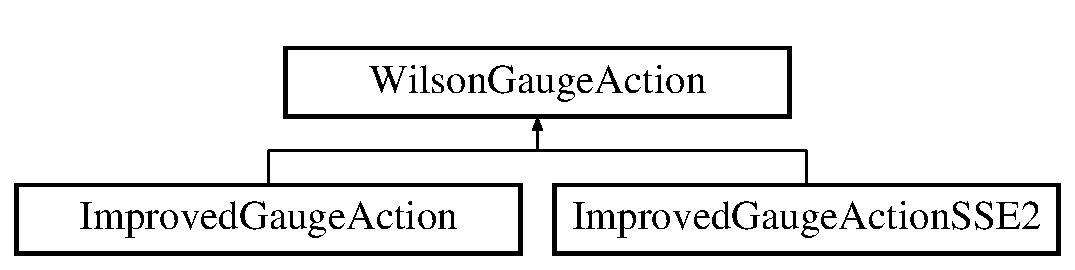
\includegraphics[height=2cm]{class_wilson_gauge_action}
\end{center}
\end{figure}
\subsection*{Static Public Member Functions}
\begin{DoxyCompactItemize}
\item 
static void \hyperlink{class_wilson_gauge_action_a95c910d9c558320e8a55ff04f330d02d}{heatbath\_\-SU2} (\hyperlink{classmdp__prng}{mdp\_\-prng} \&random, \hyperlink{mdp__global__vars_8h_a049e4c1d4e74d644878a42f9909463e4}{mdp\_\-real} beta\_\-eff, \hyperlink{classmdp__complex}{mdp\_\-complex} $\ast$a)
\item 
static \hyperlink{classgauge__stats}{gauge\_\-stats} \hyperlink{class_wilson_gauge_action_a0e5aefe5e3c15f35d0fbcd8e6269b919}{heatbath} (\hyperlink{classgauge__field}{gauge\_\-field} \&U, \hyperlink{classcoefficients}{coefficients} \&coeff, int n\_\-iter=1)
\end{DoxyCompactItemize}


\subsection{Detailed Description}
the Wilson Gauge Action Example: \begin{DoxyVerb}
///    int ns=2, steps=10;
///    gauge_field U(lattice,nc);
///    coefficients gauge;
///    U.load("myfield.0000");
///    gauge["beta"]=6.0;
///    ImprovedGaugeAction::heatbath(U,gauge,steps);
///    U.save("myfield.0001");
/// \end{DoxyVerb}
 

\subsection{Member Function Documentation}
\hypertarget{class_wilson_gauge_action_a0e5aefe5e3c15f35d0fbcd8e6269b919}{
\index{WilsonGaugeAction@{WilsonGaugeAction}!heatbath@{heatbath}}
\index{heatbath@{heatbath}!WilsonGaugeAction@{WilsonGaugeAction}}
\subsubsection[{heatbath}]{\setlength{\rightskip}{0pt plus 5cm}static {\bf gauge\_\-stats} WilsonGaugeAction::heatbath ({\bf gauge\_\-field} \& {\em U}, \/  {\bf coefficients} \& {\em coeff}, \/  int {\em n\_\-iter} = {\ttfamily 1})\hspace{0.3cm}{\ttfamily  \mbox{[}inline, static\mbox{]}}}}
\label{class_wilson_gauge_action_a0e5aefe5e3c15f35d0fbcd8e6269b919}
\hypertarget{class_wilson_gauge_action_a95c910d9c558320e8a55ff04f330d02d}{
\index{WilsonGaugeAction@{WilsonGaugeAction}!heatbath\_\-SU2@{heatbath\_\-SU2}}
\index{heatbath\_\-SU2@{heatbath\_\-SU2}!WilsonGaugeAction@{WilsonGaugeAction}}
\subsubsection[{heatbath\_\-SU2}]{\setlength{\rightskip}{0pt plus 5cm}static void WilsonGaugeAction::heatbath\_\-SU2 ({\bf mdp\_\-prng} \& {\em random}, \/  {\bf mdp\_\-real} {\em beta\_\-eff}, \/  {\bf mdp\_\-complex} $\ast$ {\em a})\hspace{0.3cm}{\ttfamily  \mbox{[}inline, static\mbox{]}}}}
\label{class_wilson_gauge_action_a95c910d9c558320e8a55ff04f330d02d}


The documentation for this class was generated from the following file:\begin{DoxyCompactItemize}
\item 
/Users/mdipierro/fermiqcd/development/Libraries/\hyperlink{fermiqcd__gauge__actions_8h}{fermiqcd\_\-gauge\_\-actions.h}\end{DoxyCompactItemize}

\hypertarget{class_wupperthal_smearing}{
\section{WupperthalSmearing Class Reference}
\label{class_wupperthal_smearing}\index{WupperthalSmearing@{WupperthalSmearing}}
}
wupperthal smearing algotihm  


{\tt \#include $<$fermiqcd\_\-fermi\_\-smearing.h$>$}



\subsection{Detailed Description}
wupperthal smearing algotihm 

Example: 

\footnotesize\begin{verbatim}
/// gauge_field U(lattice,nc);
/// fermi_field psi(lattice,nc);
/// coefficient smear;
/// smear["factor"]=2;
/// smear["steps"]=10;
/// WupperthalSmearing::smear(psi,U,spear);
/// \end{verbatim}
\normalsize
 

The documentation for this class was generated from the following file:\begin{CompactItemize}
\item 
/Users/mdipierro/Desktop/SciDac/development/Libraries/\hyperlink{fermiqcd__fermi__smearing_8h}{fermiqcd\_\-fermi\_\-smearing.h}\end{CompactItemize}

\chapter{File Documentation}
\hypertarget{average__plaquette_8cpp}{
\section{/Users/mdipierro/fermiqcd/development/Libraries/average\_\-plaquette.cpp File Reference}
\label{average__plaquette_8cpp}\index{/Users/mdipierro/fermiqcd/development/Libraries/average\_\-plaquette.cpp@{/Users/mdipierro/fermiqcd/development/Libraries/average\_\-plaquette.cpp}}
}
{\ttfamily \#include \char`\"{}fermiqcd.h\char`\"{}}\par
\subsection*{Functions}
\begin{DoxyCompactItemize}
\item 
int \hyperlink{average__plaquette_8cpp_a3c04138a5bfe5d72780bb7e82a18e627}{main} (int argc, char $\ast$$\ast$argv)
\end{DoxyCompactItemize}


\subsection{Function Documentation}
\hypertarget{average__plaquette_8cpp_a3c04138a5bfe5d72780bb7e82a18e627}{
\index{average\_\-plaquette.cpp@{average\_\-plaquette.cpp}!main@{main}}
\index{main@{main}!average_plaquette.cpp@{average\_\-plaquette.cpp}}
\subsubsection[{main}]{\setlength{\rightskip}{0pt plus 5cm}int main (int {\em argc}, \/  char $\ast$$\ast$ {\em argv})}}
\label{average__plaquette_8cpp_a3c04138a5bfe5d72780bb7e82a18e627}

\hypertarget{check__cold_8cpp}{
\section{/Users/mdipierro/fermiqcd/development/Libraries/check\_\-cold.cpp File Reference}
\label{check__cold_8cpp}\index{/Users/mdipierro/fermiqcd/development/Libraries/check\_\-cold.cpp@{/Users/mdipierro/fermiqcd/development/Libraries/check\_\-cold.cpp}}
}
{\ttfamily \#include \char`\"{}fermiqcd.h\char`\"{}}\par
\subsection*{Functions}
\begin{DoxyCompactItemize}
\item 
int \hyperlink{check__cold_8cpp_a3c04138a5bfe5d72780bb7e82a18e627}{main} (int argc, char $\ast$$\ast$argv)
\end{DoxyCompactItemize}


\subsection{Function Documentation}
\hypertarget{check__cold_8cpp_a3c04138a5bfe5d72780bb7e82a18e627}{
\index{check\_\-cold.cpp@{check\_\-cold.cpp}!main@{main}}
\index{main@{main}!check_cold.cpp@{check\_\-cold.cpp}}
\subsubsection[{main}]{\setlength{\rightskip}{0pt plus 5cm}int main (int {\em argc}, \/  char $\ast$$\ast$ {\em argv})}}
\label{check__cold_8cpp_a3c04138a5bfe5d72780bb7e82a18e627}

\hypertarget{cleanup__cpp_8py}{
\section{/Users/mdipierro/fermiqcd/development/Libraries/cleanup\_\-cpp.py File Reference}
\label{cleanup__cpp_8py}\index{/Users/mdipierro/fermiqcd/development/Libraries/cleanup\_\-cpp.py@{/Users/mdipierro/fermiqcd/development/Libraries/cleanup\_\-cpp.py}}
}
\subsection*{Namespaces}
\begin{DoxyCompactItemize}
\item 
namespace \hyperlink{namespacecleanup__cpp}{cleanup\_\-cpp}
\end{DoxyCompactItemize}
\subsection*{Functions}
\begin{DoxyCompactItemize}
\item 
def \hyperlink{namespacecleanup__cpp_a73d819752ffd659999d765cdaa2ea60b}{cleanup\_\-cpp::cleanup\_\-cpp}
\end{DoxyCompactItemize}

\hypertarget{cool__and__topological_8cpp}{
\section{/Users/mdipierro/fermiqcd/development/Libraries/cool\_\-and\_\-topological.cpp File Reference}
\label{cool__and__topological_8cpp}\index{/Users/mdipierro/fermiqcd/development/Libraries/cool\_\-and\_\-topological.cpp@{/Users/mdipierro/fermiqcd/development/Libraries/cool\_\-and\_\-topological.cpp}}
}
{\ttfamily \#include \char`\"{}fermiqcd.h\char`\"{}}\par
\subsection*{Functions}
\begin{DoxyCompactItemize}
\item 
void \hyperlink{cool__and__topological_8cpp_aabc7f2fc63cf943e2ad6e61561b9063b}{test\_\-gauge} (int nt, int nx, char $\ast$filename)
\item 
int \hyperlink{cool__and__topological_8cpp_a3c04138a5bfe5d72780bb7e82a18e627}{main} (int argc, char $\ast$$\ast$argv)
\end{DoxyCompactItemize}


\subsection{Function Documentation}
\hypertarget{cool__and__topological_8cpp_a3c04138a5bfe5d72780bb7e82a18e627}{
\index{cool\_\-and\_\-topological.cpp@{cool\_\-and\_\-topological.cpp}!main@{main}}
\index{main@{main}!cool_and_topological.cpp@{cool\_\-and\_\-topological.cpp}}
\subsubsection[{main}]{\setlength{\rightskip}{0pt plus 5cm}int main (int {\em argc}, \/  char $\ast$$\ast$ {\em argv})}}
\label{cool__and__topological_8cpp_a3c04138a5bfe5d72780bb7e82a18e627}
\hypertarget{cool__and__topological_8cpp_aabc7f2fc63cf943e2ad6e61561b9063b}{
\index{cool\_\-and\_\-topological.cpp@{cool\_\-and\_\-topological.cpp}!test\_\-gauge@{test\_\-gauge}}
\index{test\_\-gauge@{test\_\-gauge}!cool_and_topological.cpp@{cool\_\-and\_\-topological.cpp}}
\subsubsection[{test\_\-gauge}]{\setlength{\rightskip}{0pt plus 5cm}void test\_\-gauge (int {\em nt}, \/  int {\em nx}, \/  char $\ast$ {\em filename})}}
\label{cool__and__topological_8cpp_aabc7f2fc63cf943e2ad6e61561b9063b}

\hypertarget{cool__and__topological__step__by__step_8cpp}{
\section{/Users/mdipierro/fermiqcd/development/Libraries/cool\_\-and\_\-topological\_\-step\_\-by\_\-step.cpp File Reference}
\label{cool__and__topological__step__by__step_8cpp}\index{/Users/mdipierro/fermiqcd/development/Libraries/cool\_\-and\_\-topological\_\-step\_\-by\_\-step.cpp@{/Users/mdipierro/fermiqcd/development/Libraries/cool\_\-and\_\-topological\_\-step\_\-by\_\-step.cpp}}
}
{\ttfamily \#include \char`\"{}fermiqcd.h\char`\"{}}\par
\subsection*{Functions}
\begin{DoxyCompactItemize}
\item 
void \hyperlink{cool__and__topological__step__by__step_8cpp_aabc7f2fc63cf943e2ad6e61561b9063b}{test\_\-gauge} (int nt, int nx, char $\ast$filename)
\item 
int \hyperlink{cool__and__topological__step__by__step_8cpp_a3c04138a5bfe5d72780bb7e82a18e627}{main} (int argc, char $\ast$$\ast$argv)
\end{DoxyCompactItemize}


\subsection{Function Documentation}
\hypertarget{cool__and__topological__step__by__step_8cpp_a3c04138a5bfe5d72780bb7e82a18e627}{
\index{cool\_\-and\_\-topological\_\-step\_\-by\_\-step.cpp@{cool\_\-and\_\-topological\_\-step\_\-by\_\-step.cpp}!main@{main}}
\index{main@{main}!cool_and_topological_step_by_step.cpp@{cool\_\-and\_\-topological\_\-step\_\-by\_\-step.cpp}}
\subsubsection[{main}]{\setlength{\rightskip}{0pt plus 5cm}int main (int {\em argc}, \/  char $\ast$$\ast$ {\em argv})}}
\label{cool__and__topological__step__by__step_8cpp_a3c04138a5bfe5d72780bb7e82a18e627}
\hypertarget{cool__and__topological__step__by__step_8cpp_aabc7f2fc63cf943e2ad6e61561b9063b}{
\index{cool\_\-and\_\-topological\_\-step\_\-by\_\-step.cpp@{cool\_\-and\_\-topological\_\-step\_\-by\_\-step.cpp}!test\_\-gauge@{test\_\-gauge}}
\index{test\_\-gauge@{test\_\-gauge}!cool_and_topological_step_by_step.cpp@{cool\_\-and\_\-topological\_\-step\_\-by\_\-step.cpp}}
\subsubsection[{test\_\-gauge}]{\setlength{\rightskip}{0pt plus 5cm}void test\_\-gauge (int {\em nt}, \/  int {\em nx}, \/  char $\ast$ {\em filename})}}
\label{cool__and__topological__step__by__step_8cpp_aabc7f2fc63cf943e2ad6e61561b9063b}

\hypertarget{fermiqcd_8h}{
\section{/Users/mdipierro/Desktop/SciDac/development/Libraries/fermiqcd.h File Reference}
\label{fermiqcd_8h}\index{/Users/mdipierro/Desktop/SciDac/development/Libraries/fermiqcd.h@{/Users/mdipierro/Desktop/SciDac/development/Libraries/fermiqcd.h}}
}
{\tt \#include \char`\"{}mdp.h\char`\"{}}\par
{\tt \#include \char`\"{}fermiqcd\_\-global\_\-vars.h\char`\"{}}\par
{\tt \#include \char`\"{}fermiqcd\_\-gamma\_\-matrices.h\char`\"{}}\par
{\tt \#include \char`\"{}fermiqcd\_\-default\_\-parameters.h\char`\"{}}\par
{\tt \#include \char`\"{}fermiqcd\_\-check\_\-differences.h\char`\"{}}\par
{\tt \#include \char`\"{}fermiqcd\_\-set\_\-random.h\char`\"{}}\par
{\tt \#include \char`\"{}fermiqcd\_\-coefficients.h\char`\"{}}\par
{\tt \#include \char`\"{}fermiqcd\_\-sse\_\-su3.h\char`\"{}}\par
{\tt \#include \char`\"{}fermiqcd\_\-gauge\_\-field.h\char`\"{}}\par
{\tt \#include \char`\"{}fermiqcd\_\-gauge\_\-routines.h\char`\"{}}\par
{\tt \#include \char`\"{}fermiqcd\_\-gauge\_\-actions.h\char`\"{}}\par
{\tt \#include \char`\"{}fermiqcd\_\-gauge\_\-algorithms.h\char`\"{}}\par
{\tt \#include \char`\"{}fermiqcd\_\-gauge\_\-fixing.h\char`\"{}}\par
{\tt \#include \char`\"{}fermiqcd\_\-topological\_\-charge.h\char`\"{}}\par
{\tt \#include \char`\"{}fermiqcd\_\-minres\_\-inverter.h\char`\"{}}\par
{\tt \#include \char`\"{}fermiqcd\_\-bicgstab\_\-inverter.h\char`\"{}}\par
{\tt \#include \char`\"{}fermiqcd\_\-fermi\_\-field.h\char`\"{}}\par
{\tt \#include \char`\"{}fermiqcd\_\-fermi\_\-actions.h\char`\"{}}\par
{\tt \#include \char`\"{}fermiqcd\_\-fermi\_\-actions\_\-sse2.h\char`\"{}}\par
{\tt \#include \char`\"{}fermiqcd\_\-fermi\_\-algorithms.h\char`\"{}}\par
{\tt \#include \char`\"{}fermiqcd\_\-fermi\_\-propagator.h\char`\"{}}\par
{\tt \#include \char`\"{}fermiqcd\_\-fermi\_\-rotation.h\char`\"{}}\par
{\tt \#include \char`\"{}fermiqcd\_\-fermi\_\-smearing.h\char`\"{}}\par
{\tt \#include \char`\"{}fermiqcd\_\-lanczos.h\char`\"{}}\par
{\tt \#include \char`\"{}fermiqcd\_\-staggered\_\-field.h\char`\"{}}\par
{\tt \#include \char`\"{}fermiqcd\_\-staggered\_\-actions.h\char`\"{}}\par
{\tt \#include \char`\"{}fermiqcd\_\-staggered\_\-actions\_\-sse2.h\char`\"{}}\par
{\tt \#include \char`\"{}fermiqcd\_\-staggered\_\-algorithms.h\char`\"{}}\par
{\tt \#include \char`\"{}fermiqcd\_\-staggered\_\-uml\_\-inverter.h\char`\"{}}\par
{\tt \#include \char`\"{}fermiqcd\_\-staggered\_\-propagator.h\char`\"{}}\par
{\tt \#include \char`\"{}fermiqcd\_\-staggered\_\-mesons.h\char`\"{}}\par
{\tt \#include \char`\"{}fermiqcd\_\-dwfermi\_\-field.h\char`\"{}}\par
{\tt \#include \char`\"{}fermiqcd\_\-dwfermi\_\-actions.h\char`\"{}}\par
{\tt \#include \char`\"{}fermiqcd\_\-dwfermi\_\-algorithms.h\char`\"{}}\par


Include dependency graph for fermiqcd.h:

\subsection{Detailed Description}
\begin{Desc}
\item[Version:]3-1-2005 \end{Desc}
\begin{Desc}
\item[Author:]Massimo Di Pierro $<$\href{mailto:mdipierro@cs.depaul.edu}{\tt mdipierro@cs.depaul.edu}$>$\end{Desc}
Main header file for FermiQCD libraries

This file is copyrighted by Massimo Di Pierro Read attached license in file fermiqcd\_\-license.pdf This file cannot be distributed without file fermiqcd\_\-license.pdf 
\hypertarget{fermiqcd__bicgstab__inverter_8h}{
\section{/Users/mdipierro/fermiqcd/development/Libraries/fermiqcd\_\-bicgstab\_\-inverter.h File Reference}
\label{fermiqcd__bicgstab__inverter_8h}\index{/Users/mdipierro/fermiqcd/development/Libraries/fermiqcd\_\-bicgstab\_\-inverter.h@{/Users/mdipierro/fermiqcd/development/Libraries/fermiqcd\_\-bicgstab\_\-inverter.h}}
}
\subsection*{Classes}
\begin{DoxyCompactItemize}
\item 
class \hyperlink{class_bi_c_g_stab}{BiCGStab}
\begin{DoxyCompactList}\small\item\em the stabilized biconjugate inverter \item\end{DoxyCompactList}\end{DoxyCompactItemize}
\subsection*{Functions}
\begin{DoxyCompactItemize}
\item 
{\footnotesize template$<$class fieldT , class fieldG $>$ }\\\hyperlink{classinversion__stats}{inversion\_\-stats} \hyperlink{fermiqcd__bicgstab__inverter_8h_a034825adf55145e62e9312ac0e4dc80a}{BiConjugateGradientStabilizedInverter} (fieldT \&psi\_\-out, fieldT \&psi\_\-in, fieldG \&U, \hyperlink{classcoefficients}{coefficients} \&coeff, \hyperlink{mdp__global__vars_8h_a049e4c1d4e74d644878a42f9909463e4}{mdp\_\-real} absolute\_\-precision=\hyperlink{mdp__global__vars_8h_a443a4ca745298420893e113a7ac926a9}{mdp\_\-precision}, \hyperlink{mdp__global__vars_8h_a049e4c1d4e74d644878a42f9909463e4}{mdp\_\-real} relative\_\-precision=0, int max\_\-steps=2000)
\end{DoxyCompactItemize}


\subsection{Detailed Description}
\begin{DoxyVersion}{Version}
2009-\/12-\/21 
\end{DoxyVersion}
\begin{DoxyAuthor}{Author}
Massimo Di Pierro $<$\href{mailto:mdipierro@cs.depaul.edu}{\tt mdipierro@cs.depaul.edu}$>$
\end{DoxyAuthor}
Contains the stabilized biconjugate inverter From hep-\/lat/9404013 (by A. Frommer et al.)

Distributed under GPL2 License

Created with support from the US Department of Energy 

\subsection{Function Documentation}
\hypertarget{fermiqcd__bicgstab__inverter_8h_a034825adf55145e62e9312ac0e4dc80a}{
\index{fermiqcd\_\-bicgstab\_\-inverter.h@{fermiqcd\_\-bicgstab\_\-inverter.h}!BiConjugateGradientStabilizedInverter@{BiConjugateGradientStabilizedInverter}}
\index{BiConjugateGradientStabilizedInverter@{BiConjugateGradientStabilizedInverter}!fermiqcd_bicgstab_inverter.h@{fermiqcd\_\-bicgstab\_\-inverter.h}}
\subsubsection[{BiConjugateGradientStabilizedInverter}]{\setlength{\rightskip}{0pt plus 5cm}template$<$class fieldT , class fieldG $>$ {\bf inversion\_\-stats} BiConjugateGradientStabilizedInverter (fieldT \& {\em psi\_\-out}, \/  fieldT \& {\em psi\_\-in}, \/  fieldG \& {\em U}, \/  {\bf coefficients} \& {\em coeff}, \/  {\bf mdp\_\-real} {\em absolute\_\-precision} = {\ttfamily {\bf mdp\_\-precision}}, \/  {\bf mdp\_\-real} {\em relative\_\-precision} = {\ttfamily 0}, \/  int {\em max\_\-steps} = {\ttfamily 2000})\hspace{0.3cm}{\ttfamily  \mbox{[}inline\mbox{]}}}}
\label{fermiqcd__bicgstab__inverter_8h_a034825adf55145e62e9312ac0e4dc80a}

\hypertarget{fermiqcd__bicgstab__inverter__vtk_8h}{
\section{/Users/mdipierro/fermiqcd/development/Libraries/fermiqcd\_\-bicgstab\_\-inverter\_\-vtk.h File Reference}
\label{fermiqcd__bicgstab__inverter__vtk_8h}\index{/Users/mdipierro/fermiqcd/development/Libraries/fermiqcd\_\-bicgstab\_\-inverter\_\-vtk.h@{/Users/mdipierro/fermiqcd/development/Libraries/fermiqcd\_\-bicgstab\_\-inverter\_\-vtk.h}}
}
\subsection*{Classes}
\begin{DoxyCompactItemize}
\item 
class \hyperlink{class_bi_c_g_stab_vtk}{BiCGStabVtk}
\begin{DoxyCompactList}\small\item\em the stabilized biconjugate inverter \item\end{DoxyCompactList}\end{DoxyCompactItemize}
\subsection*{Functions}
\begin{DoxyCompactItemize}
\item 
{\footnotesize template$<$class fieldT , class fieldG $>$ }\\\hyperlink{classinversion__stats}{inversion\_\-stats} \hyperlink{fermiqcd__bicgstab__inverter__vtk_8h_ad5388affe9d9053678801b9395e5cdce}{BiConjugateGradientStabilizedInverterVtk} (fieldT \&psi\_\-out, fieldT \&psi\_\-in, fieldG \&U, \hyperlink{classcoefficients}{coefficients} \&coeff, \hyperlink{mdp__global__vars_8h_a049e4c1d4e74d644878a42f9909463e4}{mdp\_\-real} absolute\_\-precision=\hyperlink{mdp__global__vars_8h_a443a4ca745298420893e113a7ac926a9}{mdp\_\-precision}, \hyperlink{mdp__global__vars_8h_a049e4c1d4e74d644878a42f9909463e4}{mdp\_\-real} relative\_\-precision=0, int max\_\-steps=2000)
\end{DoxyCompactItemize}


\subsection{Function Documentation}
\hypertarget{fermiqcd__bicgstab__inverter__vtk_8h_ad5388affe9d9053678801b9395e5cdce}{
\index{fermiqcd\_\-bicgstab\_\-inverter\_\-vtk.h@{fermiqcd\_\-bicgstab\_\-inverter\_\-vtk.h}!BiConjugateGradientStabilizedInverterVtk@{BiConjugateGradientStabilizedInverterVtk}}
\index{BiConjugateGradientStabilizedInverterVtk@{BiConjugateGradientStabilizedInverterVtk}!fermiqcd_bicgstab_inverter_vtk.h@{fermiqcd\_\-bicgstab\_\-inverter\_\-vtk.h}}
\subsubsection[{BiConjugateGradientStabilizedInverterVtk}]{\setlength{\rightskip}{0pt plus 5cm}template$<$class fieldT , class fieldG $>$ {\bf inversion\_\-stats} BiConjugateGradientStabilizedInverterVtk (fieldT \& {\em psi\_\-out}, \/  fieldT \& {\em psi\_\-in}, \/  fieldG \& {\em U}, \/  {\bf coefficients} \& {\em coeff}, \/  {\bf mdp\_\-real} {\em absolute\_\-precision} = {\ttfamily {\bf mdp\_\-precision}}, \/  {\bf mdp\_\-real} {\em relative\_\-precision} = {\ttfamily 0}, \/  int {\em max\_\-steps} = {\ttfamily 2000})\hspace{0.3cm}{\ttfamily  \mbox{[}inline\mbox{]}}}}
\label{fermiqcd__bicgstab__inverter__vtk_8h_ad5388affe9d9053678801b9395e5cdce}

\hypertarget{fermiqcd__cg__inverter_8h}{
\section{/Users/mdipierro/fermiqcd/development/Libraries/fermiqcd\_\-cg\_\-inverter.h File Reference}
\label{fermiqcd__cg__inverter_8h}\index{/Users/mdipierro/fermiqcd/development/Libraries/fermiqcd\_\-cg\_\-inverter.h@{/Users/mdipierro/fermiqcd/development/Libraries/fermiqcd\_\-cg\_\-inverter.h}}
}
\subsection*{Classes}
\begin{DoxyCompactItemize}
\item 
class \hyperlink{class_c_g2}{CG2}
\begin{DoxyCompactList}\small\item\em the conjugate gradient inverter \item\end{DoxyCompactList}\end{DoxyCompactItemize}


\subsection{Detailed Description}
\begin{DoxyVersion}{Version}
5-\/8-\/2007 
\end{DoxyVersion}
\begin{DoxyAuthor}{Author}
Joseph Schneible $<$$>$ 
\end{DoxyAuthor}

\hypertarget{fermiqcd__check__differences_8h}{
\section{/Users/mdipierro/fermiqcd/development/Libraries/fermiqcd\_\-check\_\-differences.h File Reference}
\label{fermiqcd__check__differences_8h}\index{/Users/mdipierro/fermiqcd/development/Libraries/fermiqcd\_\-check\_\-differences.h@{/Users/mdipierro/fermiqcd/development/Libraries/fermiqcd\_\-check\_\-differences.h}}
}
\subsection*{Functions}
\begin{DoxyCompactItemize}
\item 
float \hyperlink{fermiqcd__check__differences_8h_adb415cfd346cc8b4d95c55a1ff3928c5}{check\_\-differences} (\hyperlink{classmdp__field}{mdp\_\-field}$<$ \hyperlink{classmdp__complex}{mdp\_\-complex} $>$ \&chi, \hyperlink{classmdp__field}{mdp\_\-field}$<$ \hyperlink{classmdp__complex}{mdp\_\-complex} $>$ \&psi)
\end{DoxyCompactItemize}


\subsection{Detailed Description}
\begin{DoxyVersion}{Version}
2009-\/12-\/21 
\end{DoxyVersion}
\begin{DoxyAuthor}{Author}
Massimo Di Pierro $<$\href{mailto:mdipierro@cs.depaul.edu}{\tt mdipierro@cs.depaul.edu}$>$
\end{DoxyAuthor}
Constants and parameters used by FermiQCD

Distributed under GPL2 License

Created with support from the US Department of Energy 

\subsection{Function Documentation}
\hypertarget{fermiqcd__check__differences_8h_adb415cfd346cc8b4d95c55a1ff3928c5}{
\index{fermiqcd\_\-check\_\-differences.h@{fermiqcd\_\-check\_\-differences.h}!check\_\-differences@{check\_\-differences}}
\index{check\_\-differences@{check\_\-differences}!fermiqcd_check_differences.h@{fermiqcd\_\-check\_\-differences.h}}
\subsubsection[{check\_\-differences}]{\setlength{\rightskip}{0pt plus 5cm}float check\_\-differences ({\bf mdp\_\-field}$<$ {\bf mdp\_\-complex} $>$ \& {\em chi}, \/  {\bf mdp\_\-field}$<$ {\bf mdp\_\-complex} $>$ \& {\em psi})}}
\label{fermiqcd__check__differences_8h_adb415cfd346cc8b4d95c55a1ff3928c5}

\hypertarget{fermiqcd__coefficients_8h}{
\section{/Users/mdipierro/Desktop/SciDac/development/Libraries/fermiqcd\_\-coefficients.h File Reference}
\label{fermiqcd__coefficients_8h}\index{/Users/mdipierro/Desktop/SciDac/development/Libraries/fermiqcd\_\-coefficients.h@{/Users/mdipierro/Desktop/SciDac/development/Libraries/fermiqcd\_\-coefficients.h}}
}


This graph shows which files directly or indirectly include this file:\subsection*{Classes}
\begin{CompactItemize}
\item 
class \hyperlink{classcoefficients}{coefficients}
\begin{CompactList}\small\item\em container for action parameters \item\end{CompactList}\end{CompactItemize}


\subsection{Detailed Description}
\begin{Desc}
\item[Version:]3-1-2005 \end{Desc}
\begin{Desc}
\item[Author:]Massimo Di Pierro $<$\href{mailto:mdipierro@cs.depaul.edu}{\tt mdipierro@cs.depaul.edu}$>$\end{Desc}
Container for action parameters

This file is copyrighted by Massimo Di Pierro Read attached license in file fermiqcd\_\-license.pdf This file cannot be distributed without file fermiqcd\_\-license.pdf 
\hypertarget{fermiqcd__default__parameters_8h}{
\section{/Users/mdipierro/fermiqcd/development/Libraries/fermiqcd\_\-default\_\-parameters.h File Reference}
\label{fermiqcd__default__parameters_8h}\index{/Users/mdipierro/fermiqcd/development/Libraries/fermiqcd\_\-default\_\-parameters.h@{/Users/mdipierro/fermiqcd/development/Libraries/fermiqcd\_\-default\_\-parameters.h}}
}
\subsection*{Defines}
\begin{DoxyCompactItemize}
\item 
\#define \hyperlink{fermiqcd__default__parameters_8h_a078b6c12f1ac6819cecef90ab5870276}{TIME}~0
\item 
\#define \hyperlink{fermiqcd__default__parameters_8h_adb697b54f3971b9c18c11b5b21800b62}{SPACE\_\-X}~1
\item 
\#define \hyperlink{fermiqcd__default__parameters_8h_afb06b9501ecbeccd8f8193c36492d86a}{SPACE\_\-Y}~2
\item 
\#define \hyperlink{fermiqcd__default__parameters_8h_a56be8433877a01427f861aa35d8f3b59}{SPACE\_\-Z}~3
\item 
\#define \hyperlink{fermiqcd__default__parameters_8h_ab6e881ccdd01e129b9aaee34137d1362}{DAGGER}~-\/1
\end{DoxyCompactItemize}
\subsection*{Variables}
\begin{DoxyCompactItemize}
\item 
\hyperlink{mdp__global__vars_8h_a049e4c1d4e74d644878a42f9909463e4}{mdp\_\-real} \hyperlink{fermiqcd__default__parameters_8h_ab11c95dc923c6bfd349bd67af277d59d}{fermi\_\-inversion\_\-precision} = 1e-\/6
\item 
\hyperlink{mdp__global__vars_8h_a049e4c1d4e74d644878a42f9909463e4}{mdp\_\-real} \hyperlink{fermiqcd__default__parameters_8h_ace2adee73e3f9d7c0df3759732b2688b}{staggered\_\-inversion\_\-precision} = 1e-\/6
\item 
\hyperlink{mdp__global__vars_8h_a049e4c1d4e74d644878a42f9909463e4}{mdp\_\-real} \hyperlink{fermiqcd__default__parameters_8h_aaf7afe8edf7318091c62707552c502ab}{dwfermi\_\-inversion\_\-precision} = 1e-\/6
\item 
\hyperlink{mdp__global__vars_8h_a049e4c1d4e74d644878a42f9909463e4}{mdp\_\-real} \hyperlink{fermiqcd__default__parameters_8h_ab987d3497c70948b4dcdf3b7f1094e27}{sdwf\_\-inversion\_\-precision} = 1e-\/6
\item 
bool \hyperlink{fermiqcd__default__parameters_8h_a9955222262f455be6cc35d1b77d4b8d9}{BiCGStabRestart} = false
\begin{DoxyCompactList}\small\item\em Set this to true to run BuCGStab with restart. \item\end{DoxyCompactList}\end{DoxyCompactItemize}


\subsection{Detailed Description}
\begin{DoxyVersion}{Version}
2009-\/12-\/21 
\end{DoxyVersion}
\begin{DoxyAuthor}{Author}
Massimo Di Pierro $<$\href{mailto:mdipierro@cs.depaul.edu}{\tt mdipierro@cs.depaul.edu}$>$
\end{DoxyAuthor}
Constants and parameters used by FermiQCD

Distributed under GPL2 License

Created with support from the US Department of Energy 

\subsection{Define Documentation}
\hypertarget{fermiqcd__default__parameters_8h_ab6e881ccdd01e129b9aaee34137d1362}{
\index{fermiqcd\_\-default\_\-parameters.h@{fermiqcd\_\-default\_\-parameters.h}!DAGGER@{DAGGER}}
\index{DAGGER@{DAGGER}!fermiqcd_default_parameters.h@{fermiqcd\_\-default\_\-parameters.h}}
\subsubsection[{DAGGER}]{\setlength{\rightskip}{0pt plus 5cm}\#define DAGGER~-\/1}}
\label{fermiqcd__default__parameters_8h_ab6e881ccdd01e129b9aaee34137d1362}
\hypertarget{fermiqcd__default__parameters_8h_adb697b54f3971b9c18c11b5b21800b62}{
\index{fermiqcd\_\-default\_\-parameters.h@{fermiqcd\_\-default\_\-parameters.h}!SPACE\_\-X@{SPACE\_\-X}}
\index{SPACE\_\-X@{SPACE\_\-X}!fermiqcd_default_parameters.h@{fermiqcd\_\-default\_\-parameters.h}}
\subsubsection[{SPACE\_\-X}]{\setlength{\rightskip}{0pt plus 5cm}\#define SPACE\_\-X~1}}
\label{fermiqcd__default__parameters_8h_adb697b54f3971b9c18c11b5b21800b62}
\hypertarget{fermiqcd__default__parameters_8h_afb06b9501ecbeccd8f8193c36492d86a}{
\index{fermiqcd\_\-default\_\-parameters.h@{fermiqcd\_\-default\_\-parameters.h}!SPACE\_\-Y@{SPACE\_\-Y}}
\index{SPACE\_\-Y@{SPACE\_\-Y}!fermiqcd_default_parameters.h@{fermiqcd\_\-default\_\-parameters.h}}
\subsubsection[{SPACE\_\-Y}]{\setlength{\rightskip}{0pt plus 5cm}\#define SPACE\_\-Y~2}}
\label{fermiqcd__default__parameters_8h_afb06b9501ecbeccd8f8193c36492d86a}
\hypertarget{fermiqcd__default__parameters_8h_a56be8433877a01427f861aa35d8f3b59}{
\index{fermiqcd\_\-default\_\-parameters.h@{fermiqcd\_\-default\_\-parameters.h}!SPACE\_\-Z@{SPACE\_\-Z}}
\index{SPACE\_\-Z@{SPACE\_\-Z}!fermiqcd_default_parameters.h@{fermiqcd\_\-default\_\-parameters.h}}
\subsubsection[{SPACE\_\-Z}]{\setlength{\rightskip}{0pt plus 5cm}\#define SPACE\_\-Z~3}}
\label{fermiqcd__default__parameters_8h_a56be8433877a01427f861aa35d8f3b59}
\hypertarget{fermiqcd__default__parameters_8h_a078b6c12f1ac6819cecef90ab5870276}{
\index{fermiqcd\_\-default\_\-parameters.h@{fermiqcd\_\-default\_\-parameters.h}!TIME@{TIME}}
\index{TIME@{TIME}!fermiqcd_default_parameters.h@{fermiqcd\_\-default\_\-parameters.h}}
\subsubsection[{TIME}]{\setlength{\rightskip}{0pt plus 5cm}\#define TIME~0}}
\label{fermiqcd__default__parameters_8h_a078b6c12f1ac6819cecef90ab5870276}


\subsection{Variable Documentation}
\hypertarget{fermiqcd__default__parameters_8h_a9955222262f455be6cc35d1b77d4b8d9}{
\index{fermiqcd\_\-default\_\-parameters.h@{fermiqcd\_\-default\_\-parameters.h}!BiCGStabRestart@{BiCGStabRestart}}
\index{BiCGStabRestart@{BiCGStabRestart}!fermiqcd_default_parameters.h@{fermiqcd\_\-default\_\-parameters.h}}
\subsubsection[{BiCGStabRestart}]{\setlength{\rightskip}{0pt plus 5cm}bool {\bf BiCGStabRestart} = false}}
\label{fermiqcd__default__parameters_8h_a9955222262f455be6cc35d1b77d4b8d9}


Set this to true to run BuCGStab with restart. \hypertarget{fermiqcd__default__parameters_8h_aaf7afe8edf7318091c62707552c502ab}{
\index{fermiqcd\_\-default\_\-parameters.h@{fermiqcd\_\-default\_\-parameters.h}!dwfermi\_\-inversion\_\-precision@{dwfermi\_\-inversion\_\-precision}}
\index{dwfermi\_\-inversion\_\-precision@{dwfermi\_\-inversion\_\-precision}!fermiqcd_default_parameters.h@{fermiqcd\_\-default\_\-parameters.h}}
\subsubsection[{dwfermi\_\-inversion\_\-precision}]{\setlength{\rightskip}{0pt plus 5cm}{\bf mdp\_\-real} {\bf dwfermi\_\-inversion\_\-precision} = 1e-\/6}}
\label{fermiqcd__default__parameters_8h_aaf7afe8edf7318091c62707552c502ab}
\hypertarget{fermiqcd__default__parameters_8h_ab11c95dc923c6bfd349bd67af277d59d}{
\index{fermiqcd\_\-default\_\-parameters.h@{fermiqcd\_\-default\_\-parameters.h}!fermi\_\-inversion\_\-precision@{fermi\_\-inversion\_\-precision}}
\index{fermi\_\-inversion\_\-precision@{fermi\_\-inversion\_\-precision}!fermiqcd_default_parameters.h@{fermiqcd\_\-default\_\-parameters.h}}
\subsubsection[{fermi\_\-inversion\_\-precision}]{\setlength{\rightskip}{0pt plus 5cm}{\bf mdp\_\-real} {\bf fermi\_\-inversion\_\-precision} = 1e-\/6}}
\label{fermiqcd__default__parameters_8h_ab11c95dc923c6bfd349bd67af277d59d}
\hypertarget{fermiqcd__default__parameters_8h_ab987d3497c70948b4dcdf3b7f1094e27}{
\index{fermiqcd\_\-default\_\-parameters.h@{fermiqcd\_\-default\_\-parameters.h}!sdwf\_\-inversion\_\-precision@{sdwf\_\-inversion\_\-precision}}
\index{sdwf\_\-inversion\_\-precision@{sdwf\_\-inversion\_\-precision}!fermiqcd_default_parameters.h@{fermiqcd\_\-default\_\-parameters.h}}
\subsubsection[{sdwf\_\-inversion\_\-precision}]{\setlength{\rightskip}{0pt plus 5cm}{\bf mdp\_\-real} {\bf sdwf\_\-inversion\_\-precision} = 1e-\/6}}
\label{fermiqcd__default__parameters_8h_ab987d3497c70948b4dcdf3b7f1094e27}
\hypertarget{fermiqcd__default__parameters_8h_ace2adee73e3f9d7c0df3759732b2688b}{
\index{fermiqcd\_\-default\_\-parameters.h@{fermiqcd\_\-default\_\-parameters.h}!staggered\_\-inversion\_\-precision@{staggered\_\-inversion\_\-precision}}
\index{staggered\_\-inversion\_\-precision@{staggered\_\-inversion\_\-precision}!fermiqcd_default_parameters.h@{fermiqcd\_\-default\_\-parameters.h}}
\subsubsection[{staggered\_\-inversion\_\-precision}]{\setlength{\rightskip}{0pt plus 5cm}{\bf mdp\_\-real} {\bf staggered\_\-inversion\_\-precision} = 1e-\/6}}
\label{fermiqcd__default__parameters_8h_ace2adee73e3f9d7c0df3759732b2688b}

\hypertarget{fermiqcd__dwfermi__actions_8h}{
\section{/Users/mdipierro/fermiqcd/development/Libraries/fermiqcd\_\-dwfermi\_\-actions.h File Reference}
\label{fermiqcd__dwfermi__actions_8h}\index{/Users/mdipierro/fermiqcd/development/Libraries/fermiqcd\_\-dwfermi\_\-actions.h@{/Users/mdipierro/fermiqcd/development/Libraries/fermiqcd\_\-dwfermi\_\-actions.h}}
}
\subsection*{Classes}
\begin{DoxyCompactItemize}
\item 
class \hyperlink{class_d_w_fermi_action_slow}{DWFermiActionSlow}
\begin{DoxyCompactList}\small\item\em domain wall action (SORRY THIS IS SLOW) \item\end{DoxyCompactList}\item 
class \hyperlink{class_d_w_fermi_action_fast}{DWFermiActionFast}
\begin{DoxyCompactList}\small\item\em domain wall action fast \item\end{DoxyCompactList}\end{DoxyCompactItemize}


\subsection{Detailed Description}
\begin{DoxyVersion}{Version}
2009-\/12-\/21 
\end{DoxyVersion}
\begin{DoxyAuthor}{Author}
Massimo Di Pierro $<$\href{mailto:mdipierro@cs.depaul.edu}{\tt mdipierro@cs.depaul.edu}$>$
\end{DoxyAuthor}
Actions for Domain Wall fermions

Distributed under GPL2 License

Created with support from the US Department of Energy 
\hypertarget{fermiqcd__dwfermi__actions__sse2_8h}{
\section{/Users/mdipierro/fermiqcd/development/Libraries/fermiqcd\_\-dwfermi\_\-actions\_\-sse2.h File Reference}
\label{fermiqcd__dwfermi__actions__sse2_8h}\index{/Users/mdipierro/fermiqcd/development/Libraries/fermiqcd\_\-dwfermi\_\-actions\_\-sse2.h@{/Users/mdipierro/fermiqcd/development/Libraries/fermiqcd\_\-dwfermi\_\-actions\_\-sse2.h}}
}

\hypertarget{fermiqcd__dwfermi__algorithms_8h}{
\section{/Users/mdipierro/Desktop/SciDac/development/Libraries/fermiqcd\_\-dwfermi\_\-algorithms.h File Reference}
\label{fermiqcd__dwfermi__algorithms_8h}\index{/Users/mdipierro/Desktop/SciDac/development/Libraries/fermiqcd\_\-dwfermi\_\-algorithms.h@{/Users/mdipierro/Desktop/SciDac/development/Libraries/fermiqcd\_\-dwfermi\_\-algorithms.h}}
}


This graph shows which files directly or indirectly include this file:\subsection*{Functions}
\begin{CompactItemize}
\item 
\hypertarget{fermiqcd__dwfermi__algorithms_8h_f09337a30c9ab6952056ececcdd50586}{
void \hyperlink{fermiqcd__dwfermi__algorithms_8h_f09337a30c9ab6952056ececcdd50586}{project} (\hyperlink{classfermi__field}{fermi\_\-field} \&psi, \hyperlink{classdwfermi__field}{dwfermi\_\-field} \&chi)}
\label{fermiqcd__dwfermi__algorithms_8h_f09337a30c9ab6952056ececcdd50586}

\begin{CompactList}\small\item\em Projects a domain wall fermion (chi) into a wilson fermion (psi). \item\end{CompactList}\item 
\hypertarget{fermiqcd__dwfermi__algorithms_8h_ef7c353f7abb7b290c85571a752a45a9}{
void \hyperlink{fermiqcd__dwfermi__algorithms_8h_ef7c353f7abb7b290c85571a752a45a9}{project} (\hyperlink{classdwfermi__field}{dwfermi\_\-field} \&chi, \hyperlink{classfermi__field}{fermi\_\-field} \&psi)}
\label{fermiqcd__dwfermi__algorithms_8h_ef7c353f7abb7b290c85571a752a45a9}

\begin{CompactList}\small\item\em Projects a will fermion (psi) into a domain wall fermion (chi). \item\end{CompactList}\item 
\hypertarget{fermiqcd__dwfermi__algorithms_8h_6260f8bdaa2ef5ac52acc067c3970877}{
void \hyperlink{fermiqcd__dwfermi__algorithms_8h_6260f8bdaa2ef5ac52acc067c3970877}{mul\_\-Q} (\hyperlink{classdwfermi__field}{dwfermi\_\-field} \&psi\_\-out, \hyperlink{classdwfermi__field}{dwfermi\_\-field} \&psi\_\-in, \hyperlink{classgauge__field}{gauge\_\-field} \&U, \hyperlink{classcoefficients}{coefficients} \&coeff)}
\label{fermiqcd__dwfermi__algorithms_8h_6260f8bdaa2ef5ac52acc067c3970877}

\begin{CompactList}\small\item\em Executes the current dwfermi action. \item\end{CompactList}\item 
\hypertarget{fermiqcd__dwfermi__algorithms_8h_726da8b698c9043b4d097cbcb07c26d8}{
\hyperlink{classinversion__stats}{inversion\_\-stats} \hyperlink{fermiqcd__dwfermi__algorithms_8h_726da8b698c9043b4d097cbcb07c26d8}{mul\_\-invQ} (\hyperlink{classdwfermi__field}{dwfermi\_\-field} \&psi\_\-out, \hyperlink{classdwfermi__field}{dwfermi\_\-field} \&psi\_\-in, \hyperlink{classgauge__field}{gauge\_\-field} \&U, \hyperlink{classcoefficients}{coefficients} \&coeff, mdp\_\-real absolute\_\-precision=dwfermi\_\-inversion\_\-precision, mdp\_\-real relative\_\-precision=0, int max\_\-steps=2000)}
\label{fermiqcd__dwfermi__algorithms_8h_726da8b698c9043b4d097cbcb07c26d8}

\begin{CompactList}\small\item\em Execute the default dwfermi inverter. \item\end{CompactList}\end{CompactItemize}
\subsection*{Variables}
\begin{CompactItemize}
\item 
\hypertarget{fermiqcd__dwfermi__algorithms_8h_f088150be92b922295701f4bec9f620e}{
void($\ast$ \hyperlink{fermiqcd__dwfermi__algorithms_8h_f088150be92b922295701f4bec9f620e}{default\_\-dwfermi\_\-action} )(\hyperlink{classdwfermi__field}{dwfermi\_\-field} \&, \hyperlink{classdwfermi__field}{dwfermi\_\-field} \&, \hyperlink{classgauge__field}{gauge\_\-field} \&, \hyperlink{classcoefficients}{coefficients} \&) = DWFermiActionFast::mul\_\-Q}
\label{fermiqcd__dwfermi__algorithms_8h_f088150be92b922295701f4bec9f620e}

\begin{CompactList}\small\item\em Pointer to the current dwfermi action. \item\end{CompactList}\item 
\hypertarget{fermiqcd__dwfermi__algorithms_8h_c92f51728e6fa5115e74a60e810bbfad}{
\hyperlink{classinversion__stats}{inversion\_\-stats}($\ast$ \hyperlink{fermiqcd__dwfermi__algorithms_8h_c92f51728e6fa5115e74a60e810bbfad}{default\_\-dwfermi\_\-inverter} )(\hyperlink{classdwfermi__field}{dwfermi\_\-field} \&, \hyperlink{classdwfermi__field}{dwfermi\_\-field} \&, \hyperlink{classgauge__field}{gauge\_\-field} \&, \hyperlink{classcoefficients}{coefficients} \&, mdp\_\-real, mdp\_\-real, int)}
\label{fermiqcd__dwfermi__algorithms_8h_c92f51728e6fa5115e74a60e810bbfad}

\begin{CompactList}\small\item\em Pointer to the current dwfermi inverter. \item\end{CompactList}\end{CompactItemize}


\subsection{Detailed Description}
\begin{Desc}
\item[Version:]3-1-2005 \end{Desc}
\begin{Desc}
\item[Author:]Massimo Di Pierro $<$\href{mailto:mdipierro@cs.depaul.edu}{\tt mdipierro@cs.depaul.edu}$>$\end{Desc}
More stuff for domain wall fermions

This file is copyrighted by Massimo Di Pierro Read attached license in file fermiqcd\_\-license.pdf This file cannot be distributed without file fermiqcd\_\-license.pdf 
\hypertarget{fermiqcd__dwfermi__field_8h}{
\section{/Users/mdipierro/fermiqcd/development/Libraries/fermiqcd\_\-dwfermi\_\-field.h File Reference}
\label{fermiqcd__dwfermi__field_8h}\index{/Users/mdipierro/fermiqcd/development/Libraries/fermiqcd\_\-dwfermi\_\-field.h@{/Users/mdipierro/fermiqcd/development/Libraries/fermiqcd\_\-dwfermi\_\-field.h}}
}
\subsection*{Classes}
\begin{DoxyCompactItemize}
\item 
class \hyperlink{classdwfermi__field}{dwfermi\_\-field}
\begin{DoxyCompactList}\small\item\em domain wall fermionic field \item\end{DoxyCompactList}\end{DoxyCompactItemize}


\subsection{Detailed Description}
\begin{DoxyVersion}{Version}
2009-\/12-\/21 
\end{DoxyVersion}
\begin{DoxyAuthor}{Author}
Massimo Di Pierro $<$\href{mailto:mdipierro@cs.depaul.edu}{\tt mdipierro@cs.depaul.edu}$>$
\end{DoxyAuthor}
Contains the class \hyperlink{classdwfermi__field}{dwfermi\_\-field} fro domain wall fermions

Distributed under GPL2 License

Created with support from the US Department of Energy 
\hypertarget{fermiqcd__fermi__actions_8h}{
\section{/Users/mdipierro/fermiqcd/development/Libraries/fermiqcd\_\-fermi\_\-actions.h File Reference}
\label{fermiqcd__fermi__actions_8h}\index{/Users/mdipierro/fermiqcd/development/Libraries/fermiqcd\_\-fermi\_\-actions.h@{/Users/mdipierro/fermiqcd/development/Libraries/fermiqcd\_\-fermi\_\-actions.h}}
}
\subsection*{Classes}
\begin{DoxyCompactItemize}
\item 
class \hyperlink{class_fermi_clover_action_slow}{FermiCloverActionSlow}
\begin{DoxyCompactList}\small\item\em Wilson/Clover action (SLOW: DO NOT USE IN PRODUCTION). \item\end{DoxyCompactList}\item 
class \hyperlink{class_fermi_clover_action_fast}{FermiCloverActionFast}
\begin{DoxyCompactList}\small\item\em Wilson/Clover action. \item\end{DoxyCompactList}\end{DoxyCompactItemize}


\subsection{Detailed Description}
\begin{DoxyVersion}{Version}
2009-\/12-\/21 
\end{DoxyVersion}
\begin{DoxyAuthor}{Author}
Massimo Di Pierro $<$\href{mailto:mdipierro@cs.depaul.edu}{\tt mdipierro@cs.depaul.edu}$>$
\end{DoxyAuthor}
Basic actions for Wilson Fermions

Distributed under GPL2 License

Created with support from the US Department of Energy 
\hypertarget{fermiqcd__fermi__actions__sse2_8h}{
\section{/Users/mdipierro/Desktop/SciDac/development/Libraries/fermiqcd\_\-fermi\_\-actions\_\-sse2.h File Reference}
\label{fermiqcd__fermi__actions__sse2_8h}\index{/Users/mdipierro/Desktop/SciDac/development/Libraries/fermiqcd\_\-fermi\_\-actions\_\-sse2.h@{/Users/mdipierro/Desktop/SciDac/development/Libraries/fermiqcd\_\-fermi\_\-actions\_\-sse2.h}}
}


This graph shows which files directly or indirectly include this file:

\subsection{Detailed Description}
\begin{Desc}
\item[Version:]3-1-2005 \end{Desc}
\begin{Desc}
\item[Author:]Martin Luescher and Massimo Di Pierro $<$\href{mailto:mdipierro@cs.depaul.edu}{\tt mdipierro@cs.depaul.edu}$>$\end{Desc}
Basic actions for Wilson Fermions optimized in assembler 
\hypertarget{fermiqcd__fermi__algorithms_8h}{
\section{/Users/mdipierro/fermiqcd/development/Libraries/fermiqcd\_\-fermi\_\-algorithms.h File Reference}
\label{fermiqcd__fermi__algorithms_8h}\index{/Users/mdipierro/fermiqcd/development/Libraries/fermiqcd\_\-fermi\_\-algorithms.h@{/Users/mdipierro/fermiqcd/development/Libraries/fermiqcd\_\-fermi\_\-algorithms.h}}
}
\subsection*{Functions}
\begin{DoxyCompactItemize}
\item 
void \hyperlink{fermiqcd__fermi__algorithms_8h_a96c52f990c5198131f211858de4e34e3}{multiply\_\-by\_\-gamma5} (\hyperlink{classfermi__field}{fermi\_\-field} \&r, \hyperlink{classfermi__field}{fermi\_\-field} \&s)
\begin{DoxyCompactList}\small\item\em r(x,alpha,i) = Gamma5(alpha,beta) $\ast$ s(x,beta,i) \item\end{DoxyCompactList}\item 
void \hyperlink{fermiqcd__fermi__algorithms_8h_aea9ab5572df48adcbfe726881033b9b5}{mul\_\-Q} (\hyperlink{classfermi__field}{fermi\_\-field} \&psi\_\-out, \hyperlink{classfermi__field}{fermi\_\-field} \&psi\_\-in, \hyperlink{classgauge__field}{gauge\_\-field} \&U, \hyperlink{classcoefficients}{coefficients} \&coeff, int parity=\hyperlink{mdp__global__vars_8h_a4c9de81f2de5a74b588107b6c0afb9ee}{EVENODD})
\begin{DoxyCompactList}\small\item\em Calls the current Wilson/Clover action. \item\end{DoxyCompactList}\item 
\hyperlink{classinversion__stats}{inversion\_\-stats} \hyperlink{fermiqcd__fermi__algorithms_8h_a08f2dd58e150767f1457309f400b860e}{mul\_\-invQ} (\hyperlink{classfermi__field}{fermi\_\-field} \&psi\_\-out, \hyperlink{classfermi__field}{fermi\_\-field} \&psi\_\-in, \hyperlink{classgauge__field}{gauge\_\-field} \&U, \hyperlink{classcoefficients}{coefficients} \&coeff, \hyperlink{mdp__global__vars_8h_a049e4c1d4e74d644878a42f9909463e4}{mdp\_\-real} absolute\_\-precision=\hyperlink{fermiqcd__default__parameters_8h_ab11c95dc923c6bfd349bd67af277d59d}{fermi\_\-inversion\_\-precision}, \hyperlink{mdp__global__vars_8h_a049e4c1d4e74d644878a42f9909463e4}{mdp\_\-real} relative\_\-precision=0, int max\_\-steps=2000)
\begin{DoxyCompactList}\small\item\em Executes the current Wilson/Clover inverter. \item\end{DoxyCompactList}\item 
\hyperlink{mdp__global__vars_8h_a049e4c1d4e74d644878a42f9909463e4}{mdp\_\-real} \hyperlink{fermiqcd__fermi__algorithms_8h_afcb44574a7920934e47a2c656e65c666}{check\_\-inversion} (\hyperlink{classfermi__field}{fermi\_\-field} \&phi, \hyperlink{classgauge__field}{gauge\_\-field} \&U, \hyperlink{classcoefficients}{coefficients} \&coeff)
\begin{DoxyCompactList}\small\item\em Checks that inversion is working. \item\end{DoxyCompactList}\end{DoxyCompactItemize}
\subsection*{Variables}
\begin{DoxyCompactItemize}
\item 
void($\ast$ \hyperlink{fermiqcd__fermi__algorithms_8h_a031121893ccfb8b423afc74855837f81}{default\_\-fermi\_\-action} )(\hyperlink{classfermi__field}{fermi\_\-field} \&, \hyperlink{classfermi__field}{fermi\_\-field} \&, \hyperlink{classgauge__field}{gauge\_\-field} \&, \hyperlink{classcoefficients}{coefficients} \&, int) = FermiCloverActionFast::mul\_\-Q
\begin{DoxyCompactList}\small\item\em Pointer to the current Wilson/Clover action. \item\end{DoxyCompactList}\item 
\hyperlink{classinversion__stats}{inversion\_\-stats}($\ast$ \hyperlink{fermiqcd__fermi__algorithms_8h_a4b9873faae44ed788d8c2925f5428535}{default\_\-fermi\_\-inverter} )(\hyperlink{classfermi__field}{fermi\_\-field} \&, \hyperlink{classfermi__field}{fermi\_\-field} \&, \hyperlink{classgauge__field}{gauge\_\-field} \&, \hyperlink{classcoefficients}{coefficients} \&, \hyperlink{mdp__global__vars_8h_a049e4c1d4e74d644878a42f9909463e4}{mdp\_\-real}, \hyperlink{mdp__global__vars_8h_a049e4c1d4e74d644878a42f9909463e4}{mdp\_\-real}, int) = \&(MinRes::inverter$<$\hyperlink{classfermi__field}{fermi\_\-field},\hyperlink{classgauge__field}{gauge\_\-field}$>$)
\begin{DoxyCompactList}\small\item\em Pointer to the current Wilson/Clover inverter. \item\end{DoxyCompactList}\end{DoxyCompactItemize}


\subsection{Detailed Description}
\begin{DoxyVersion}{Version}
2009-\/12-\/21 
\end{DoxyVersion}
\begin{DoxyAuthor}{Author}
Massimo Di Pierro $<$\href{mailto:mdipierro@cs.depaul.edu}{\tt mdipierro@cs.depaul.edu}$>$
\end{DoxyAuthor}
Various algorithms for Wilson fermions

Distributed under GPL2 License

Created with support from the US Department of Energy

\begin{DoxyVersion}{Version}
2009-\/12-\/21 
\end{DoxyVersion}
\begin{DoxyAuthor}{Author}
Massimo Di Pierro $<$\href{mailto:mdipierro@cs.depaul.edu}{\tt mdipierro@cs.depaul.edu}$>$
\end{DoxyAuthor}
class for building a single instanton gauge configuration

Distributed under GPL2 License

Created with support from the US Department of Energy 

\subsection{Function Documentation}
\hypertarget{fermiqcd__fermi__algorithms_8h_afcb44574a7920934e47a2c656e65c666}{
\index{fermiqcd\_\-fermi\_\-algorithms.h@{fermiqcd\_\-fermi\_\-algorithms.h}!check\_\-inversion@{check\_\-inversion}}
\index{check\_\-inversion@{check\_\-inversion}!fermiqcd_fermi_algorithms.h@{fermiqcd\_\-fermi\_\-algorithms.h}}
\subsubsection[{check\_\-inversion}]{\setlength{\rightskip}{0pt plus 5cm}{\bf mdp\_\-real} check\_\-inversion ({\bf fermi\_\-field} \& {\em phi}, \/  {\bf gauge\_\-field} \& {\em U}, \/  {\bf coefficients} \& {\em coeff})}}
\label{fermiqcd__fermi__algorithms_8h_afcb44574a7920934e47a2c656e65c666}


Checks that inversion is working. \hypertarget{fermiqcd__fermi__algorithms_8h_a08f2dd58e150767f1457309f400b860e}{
\index{fermiqcd\_\-fermi\_\-algorithms.h@{fermiqcd\_\-fermi\_\-algorithms.h}!mul\_\-invQ@{mul\_\-invQ}}
\index{mul\_\-invQ@{mul\_\-invQ}!fermiqcd_fermi_algorithms.h@{fermiqcd\_\-fermi\_\-algorithms.h}}
\subsubsection[{mul\_\-invQ}]{\setlength{\rightskip}{0pt plus 5cm}{\bf inversion\_\-stats} mul\_\-invQ ({\bf fermi\_\-field} \& {\em psi\_\-out}, \/  {\bf fermi\_\-field} \& {\em psi\_\-in}, \/  {\bf gauge\_\-field} \& {\em U}, \/  {\bf coefficients} \& {\em coeff}, \/  {\bf mdp\_\-real} {\em absolute\_\-precision} = {\ttfamily {\bf fermi\_\-inversion\_\-precision}}, \/  {\bf mdp\_\-real} {\em relative\_\-precision} = {\ttfamily 0}, \/  int {\em max\_\-steps} = {\ttfamily 2000})}}
\label{fermiqcd__fermi__algorithms_8h_a08f2dd58e150767f1457309f400b860e}


Executes the current Wilson/Clover inverter. \hypertarget{fermiqcd__fermi__algorithms_8h_aea9ab5572df48adcbfe726881033b9b5}{
\index{fermiqcd\_\-fermi\_\-algorithms.h@{fermiqcd\_\-fermi\_\-algorithms.h}!mul\_\-Q@{mul\_\-Q}}
\index{mul\_\-Q@{mul\_\-Q}!fermiqcd_fermi_algorithms.h@{fermiqcd\_\-fermi\_\-algorithms.h}}
\subsubsection[{mul\_\-Q}]{\setlength{\rightskip}{0pt plus 5cm}void mul\_\-Q ({\bf fermi\_\-field} \& {\em psi\_\-out}, \/  {\bf fermi\_\-field} \& {\em psi\_\-in}, \/  {\bf gauge\_\-field} \& {\em U}, \/  {\bf coefficients} \& {\em coeff}, \/  int {\em parity} = {\ttfamily {\bf EVENODD}})}}
\label{fermiqcd__fermi__algorithms_8h_aea9ab5572df48adcbfe726881033b9b5}


Calls the current Wilson/Clover action. \hypertarget{fermiqcd__fermi__algorithms_8h_a96c52f990c5198131f211858de4e34e3}{
\index{fermiqcd\_\-fermi\_\-algorithms.h@{fermiqcd\_\-fermi\_\-algorithms.h}!multiply\_\-by\_\-gamma5@{multiply\_\-by\_\-gamma5}}
\index{multiply\_\-by\_\-gamma5@{multiply\_\-by\_\-gamma5}!fermiqcd_fermi_algorithms.h@{fermiqcd\_\-fermi\_\-algorithms.h}}
\subsubsection[{multiply\_\-by\_\-gamma5}]{\setlength{\rightskip}{0pt plus 5cm}void multiply\_\-by\_\-gamma5 ({\bf fermi\_\-field} \& {\em r}, \/  {\bf fermi\_\-field} \& {\em s})}}
\label{fermiqcd__fermi__algorithms_8h_a96c52f990c5198131f211858de4e34e3}


r(x,alpha,i) = Gamma5(alpha,beta) $\ast$ s(x,beta,i) 

\subsection{Variable Documentation}
\hypertarget{fermiqcd__fermi__algorithms_8h_a031121893ccfb8b423afc74855837f81}{
\index{fermiqcd\_\-fermi\_\-algorithms.h@{fermiqcd\_\-fermi\_\-algorithms.h}!default\_\-fermi\_\-action@{default\_\-fermi\_\-action}}
\index{default\_\-fermi\_\-action@{default\_\-fermi\_\-action}!fermiqcd_fermi_algorithms.h@{fermiqcd\_\-fermi\_\-algorithms.h}}
\subsubsection[{default\_\-fermi\_\-action}]{\setlength{\rightskip}{0pt plus 5cm}void($\ast$ {\bf default\_\-fermi\_\-action})({\bf fermi\_\-field} \&, {\bf fermi\_\-field} \&, {\bf gauge\_\-field} \&, {\bf coefficients} \&, int) = FermiCloverActionFast::mul\_\-Q}}
\label{fermiqcd__fermi__algorithms_8h_a031121893ccfb8b423afc74855837f81}


Pointer to the current Wilson/Clover action. \hypertarget{fermiqcd__fermi__algorithms_8h_a4b9873faae44ed788d8c2925f5428535}{
\index{fermiqcd\_\-fermi\_\-algorithms.h@{fermiqcd\_\-fermi\_\-algorithms.h}!default\_\-fermi\_\-inverter@{default\_\-fermi\_\-inverter}}
\index{default\_\-fermi\_\-inverter@{default\_\-fermi\_\-inverter}!fermiqcd_fermi_algorithms.h@{fermiqcd\_\-fermi\_\-algorithms.h}}
\subsubsection[{default\_\-fermi\_\-inverter}]{\setlength{\rightskip}{0pt plus 5cm}{\bf inversion\_\-stats}($\ast$ {\bf default\_\-fermi\_\-inverter})({\bf fermi\_\-field} \&, {\bf fermi\_\-field} \&, {\bf gauge\_\-field} \&, {\bf coefficients} \&, {\bf mdp\_\-real}, {\bf mdp\_\-real}, int) = \&(MinRes::inverter$<${\bf fermi\_\-field},{\bf gauge\_\-field}$>$)}}
\label{fermiqcd__fermi__algorithms_8h_a4b9873faae44ed788d8c2925f5428535}


Pointer to the current Wilson/Clover inverter. 
\hypertarget{fermiqcd__fermi__field_8h}{
\section{/Users/mdipierro/fermiqcd/development/Libraries/fermiqcd\_\-fermi\_\-field.h File Reference}
\label{fermiqcd__fermi__field_8h}\index{/Users/mdipierro/fermiqcd/development/Libraries/fermiqcd\_\-fermi\_\-field.h@{/Users/mdipierro/fermiqcd/development/Libraries/fermiqcd\_\-fermi\_\-field.h}}
}
\subsection*{Classes}
\begin{DoxyCompactItemize}
\item 
class \hyperlink{classfermi__field}{fermi\_\-field}
\begin{DoxyCompactList}\small\item\em wilson fermionic field \item\end{DoxyCompactList}\end{DoxyCompactItemize}
\subsection*{Functions}
\begin{DoxyCompactItemize}
\item 
void \hyperlink{fermiqcd__fermi__field_8h_aac72e6c3c46107dcfb23a4b2cd456630}{print\_\-fermi\_\-field} (\hyperlink{classfermi__field}{fermi\_\-field} \&psi)
\end{DoxyCompactItemize}


\subsection{Detailed Description}
\begin{DoxyVersion}{Version}
2009-\/12-\/21 
\end{DoxyVersion}
\begin{DoxyAuthor}{Author}
Massimo Di Pierro $<$\href{mailto:mdipierro@cs.depaul.edu}{\tt mdipierro@cs.depaul.edu}$>$
\end{DoxyAuthor}
Contains the class \hyperlink{classfermi__field}{fermi\_\-field}

Distributed under GPL2 License

Created with support from the US Department of Energy 

\subsection{Function Documentation}
\hypertarget{fermiqcd__fermi__field_8h_aac72e6c3c46107dcfb23a4b2cd456630}{
\index{fermiqcd\_\-fermi\_\-field.h@{fermiqcd\_\-fermi\_\-field.h}!print\_\-fermi\_\-field@{print\_\-fermi\_\-field}}
\index{print\_\-fermi\_\-field@{print\_\-fermi\_\-field}!fermiqcd_fermi_field.h@{fermiqcd\_\-fermi\_\-field.h}}
\subsubsection[{print\_\-fermi\_\-field}]{\setlength{\rightskip}{0pt plus 5cm}void print\_\-fermi\_\-field ({\bf fermi\_\-field} \& {\em psi})}}
\label{fermiqcd__fermi__field_8h_aac72e6c3c46107dcfb23a4b2cd456630}

\hypertarget{fermiqcd__fermi__propagator_8h}{
\section{/Users/mdipierro/fermiqcd/development/Libraries/fermiqcd\_\-fermi\_\-propagator.h File Reference}
\label{fermiqcd__fermi__propagator_8h}\index{/Users/mdipierro/fermiqcd/development/Libraries/fermiqcd\_\-fermi\_\-propagator.h@{/Users/mdipierro/fermiqcd/development/Libraries/fermiqcd\_\-fermi\_\-propagator.h}}
}
\subsection*{Classes}
\begin{DoxyCompactItemize}
\item 
class \hyperlink{classfermi__propagator}{fermi\_\-propagator}
\begin{DoxyCompactList}\small\item\em a Wilson/Clover quark propagator (all 12 components) \item\end{DoxyCompactList}\end{DoxyCompactItemize}
\subsection*{Functions}
\begin{DoxyCompactItemize}
\item 
void \hyperlink{fermiqcd__fermi__propagator_8h_a98cfb03741c5678baa92c0fcd524ca36}{print\_\-propagator} (\hyperlink{classfermi__propagator}{fermi\_\-propagator} \&S)
\end{DoxyCompactItemize}


\subsection{Detailed Description}
\begin{DoxyVersion}{Version}
2009-\/12-\/21 
\end{DoxyVersion}
\begin{DoxyAuthor}{Author}
Massimo Di Pierro $<$\href{mailto:mdipierro@cs.depaul.edu}{\tt mdipierro@cs.depaul.edu}$>$
\end{DoxyAuthor}
Contains class \hyperlink{classfermi__propagator}{fermi\_\-propagator}

Distributed under GPL2 License

Created with support from the US Department of Energy 

\subsection{Function Documentation}
\hypertarget{fermiqcd__fermi__propagator_8h_a98cfb03741c5678baa92c0fcd524ca36}{
\index{fermiqcd\_\-fermi\_\-propagator.h@{fermiqcd\_\-fermi\_\-propagator.h}!print\_\-propagator@{print\_\-propagator}}
\index{print\_\-propagator@{print\_\-propagator}!fermiqcd_fermi_propagator.h@{fermiqcd\_\-fermi\_\-propagator.h}}
\subsubsection[{print\_\-propagator}]{\setlength{\rightskip}{0pt plus 5cm}void print\_\-propagator ({\bf fermi\_\-propagator} \& {\em S})}}
\label{fermiqcd__fermi__propagator_8h_a98cfb03741c5678baa92c0fcd524ca36}

\hypertarget{fermiqcd__fermi__rotation_8h}{
\section{/Users/mdipierro/fermiqcd/development/Libraries/fermiqcd\_\-fermi\_\-rotation.h File Reference}
\label{fermiqcd__fermi__rotation_8h}\index{/Users/mdipierro/fermiqcd/development/Libraries/fermiqcd\_\-fermi\_\-rotation.h@{/Users/mdipierro/fermiqcd/development/Libraries/fermiqcd\_\-fermi\_\-rotation.h}}
}
\subsection*{Functions}
\begin{DoxyCompactItemize}
\item 
void \hyperlink{fermiqcd__fermi__rotation_8h_a32bb10ba8cfa6ba9cbd8064665a10619}{rotate\_\-field} (\hyperlink{classfermi__field}{fermi\_\-field} \&psi, \hyperlink{classgauge__field}{gauge\_\-field} \&U, \hyperlink{classcoefficients}{coefficients} \&coeff)
\end{DoxyCompactItemize}


\subsection{Function Documentation}
\hypertarget{fermiqcd__fermi__rotation_8h_a32bb10ba8cfa6ba9cbd8064665a10619}{
\index{fermiqcd\_\-fermi\_\-rotation.h@{fermiqcd\_\-fermi\_\-rotation.h}!rotate\_\-field@{rotate\_\-field}}
\index{rotate\_\-field@{rotate\_\-field}!fermiqcd_fermi_rotation.h@{fermiqcd\_\-fermi\_\-rotation.h}}
\subsubsection[{rotate\_\-field}]{\setlength{\rightskip}{0pt plus 5cm}void rotate\_\-field ({\bf fermi\_\-field} \& {\em psi}, \/  {\bf gauge\_\-field} \& {\em U}, \/  {\bf coefficients} \& {\em coeff})}}
\label{fermiqcd__fermi__rotation_8h_a32bb10ba8cfa6ba9cbd8064665a10619}

\hypertarget{fermiqcd__fermi__smearing_8h}{
\section{/Users/mdipierro/fermiqcd/development/Libraries/fermiqcd\_\-fermi\_\-smearing.h File Reference}
\label{fermiqcd__fermi__smearing_8h}\index{/Users/mdipierro/fermiqcd/development/Libraries/fermiqcd\_\-fermi\_\-smearing.h@{/Users/mdipierro/fermiqcd/development/Libraries/fermiqcd\_\-fermi\_\-smearing.h}}
}
\subsection*{Classes}
\begin{DoxyCompactItemize}
\item 
class \hyperlink{class_wupperthal_smearing}{WupperthalSmearing}
\begin{DoxyCompactList}\small\item\em wupperthal smearing algotihm \item\end{DoxyCompactList}\end{DoxyCompactItemize}
\subsection*{Functions}
\begin{DoxyCompactItemize}
\item 
void \hyperlink{fermiqcd__fermi__smearing_8h_ad6b821559a2bc8b125bf28a441666fd6}{smearSink} (\hyperlink{classfermi__propagator}{fermi\_\-propagator} \&S, \hyperlink{classgauge__field}{gauge\_\-field} \&U, void($\ast$smf)(\hyperlink{classfermi__field}{fermi\_\-field} \&, \hyperlink{classgauge__field}{gauge\_\-field} \&, \hyperlink{classcoefficients}{coefficients} \&), \hyperlink{classcoefficients}{coefficients} \&coeff)
\begin{DoxyCompactList}\small\item\em smears a propagator \item\end{DoxyCompactList}\end{DoxyCompactItemize}


\subsection{Detailed Description}
\begin{DoxyVersion}{Version}
2009-\/12-\/21 
\end{DoxyVersion}
\begin{DoxyAuthor}{Author}
Massimo Di Pierro $<$\href{mailto:mdipierro@cs.depaul.edu}{\tt mdipierro@cs.depaul.edu}$>$
\end{DoxyAuthor}
Smearing algorithms

Distributed under GPL2 License

Created with support from the US Department of Energy 

\subsection{Function Documentation}
\hypertarget{fermiqcd__fermi__smearing_8h_ad6b821559a2bc8b125bf28a441666fd6}{
\index{fermiqcd\_\-fermi\_\-smearing.h@{fermiqcd\_\-fermi\_\-smearing.h}!smearSink@{smearSink}}
\index{smearSink@{smearSink}!fermiqcd_fermi_smearing.h@{fermiqcd\_\-fermi\_\-smearing.h}}
\subsubsection[{smearSink}]{\setlength{\rightskip}{0pt plus 5cm}void smearSink ({\bf fermi\_\-propagator} \& {\em S}, \/  {\bf gauge\_\-field} \& {\em U}, \/  void($\ast$)({\bf fermi\_\-field} \&, {\bf gauge\_\-field} \&, {\bf coefficients} \&) {\em smf}, \/  {\bf coefficients} \& {\em coeff})}}
\label{fermiqcd__fermi__smearing_8h_ad6b821559a2bc8b125bf28a441666fd6}


smears a propagator 
\hypertarget{fermiqcd__fermilab__action_8h}{
\section{/Users/mdipierro/Desktop/SciDac/development/Libraries/fermiqcd\_\-fermilab\_\-action.h File Reference}
\label{fermiqcd__fermilab__action_8h}\index{/Users/mdipierro/Desktop/SciDac/development/Libraries/fermiqcd\_\-fermilab\_\-action.h@{/Users/mdipierro/Desktop/SciDac/development/Libraries/fermiqcd\_\-fermilab\_\-action.h}}
}


\subsection{Detailed Description}
\begin{Desc}
\item[Version:]3-1-2005 \end{Desc}
\begin{Desc}
\item[Author:]Massimo Di Pierro $<$\href{mailto:mdipierro@cs.depaul.edu}{\tt mdipierro@cs.depaul.edu}$>$\end{Desc}
Fermilab action with all dimension 5 and 6 terms (requires SSE)

This file is copyrighted by Massimo Di Pierro Read attached license in file fermiqcd\_\-license.pdf This file cannot be distributed without file fermiqcd\_\-license.pdf 
\hypertarget{fermiqcd__fermilab__coefficients_8h}{
\section{/Users/mdipierro/Desktop/SciDac/development/Libraries/fermiqcd\_\-fermilab\_\-coefficients.h File Reference}
\label{fermiqcd__fermilab__coefficients_8h}\index{/Users/mdipierro/Desktop/SciDac/development/Libraries/fermiqcd\_\-fermilab\_\-coefficients.h@{/Users/mdipierro/Desktop/SciDac/development/Libraries/fermiqcd\_\-fermilab\_\-coefficients.h}}
}


\subsection{Detailed Description}
\begin{Desc}
\item[Version:]3-1-2005 \end{Desc}
\begin{Desc}
\item[Author:]Massimo Di Pierro $<$\href{mailto:mdipierro@cs.depaul.edu}{\tt mdipierro@cs.depaul.edu}$>$\end{Desc}
Included by \hyperlink{fermiqcd__fermilab__action_8h}{fermiqcd\_\-fermilab\_\-action.h}

This file is copyrighted by Massimo Di Pierro Read attached license in file fermiqcd\_\-license.pdf This file cannot be distributed without file fermiqcd\_\-license.pdf 
\hypertarget{fermiqcd__ffts_8h}{
\section{/Users/mdipierro/fermiqcd/development/Libraries/fermiqcd\_\-ffts.h File Reference}
\label{fermiqcd__ffts_8h}\index{/Users/mdipierro/fermiqcd/development/Libraries/fermiqcd\_\-ffts.h@{/Users/mdipierro/fermiqcd/development/Libraries/fermiqcd\_\-ffts.h}}
}
\subsection*{Functions}
\begin{DoxyCompactItemize}
\item 
\hyperlink{mdp__global__vars_8h_aaa1ad9d0dcd2124aa5af0120d9954174}{mdp\_\-int} \hyperlink{fermiqcd__ffts_8h_ab515049f2fa55081ae972a17afaa2956}{i2pow} (\hyperlink{mdp__global__vars_8h_aaa1ad9d0dcd2124aa5af0120d9954174}{mdp\_\-int} n)
\item 
void \hyperlink{fermiqcd__ffts_8h_a0a7bc08dfd21872b8513519f50ef2e82}{dft} (\hyperlink{classmdp__complex}{mdp\_\-complex} $\ast$fft\_\-f, \hyperlink{classmdp__complex}{mdp\_\-complex} $\ast$f, \hyperlink{mdp__global__vars_8h_aaa1ad9d0dcd2124aa5af0120d9954174}{mdp\_\-int} n, double sign, \hyperlink{mdp__global__vars_8h_aaa1ad9d0dcd2124aa5af0120d9954174}{mdp\_\-int} offset=0, \hyperlink{mdp__global__vars_8h_aaa1ad9d0dcd2124aa5af0120d9954174}{mdp\_\-int} coeff=1)
\item 
void \hyperlink{fermiqcd__ffts_8h_abef397601c3dec514364e47c6547922d}{fermi\_\-field\_\-fft} (int t, \hyperlink{classfermi__field}{fermi\_\-field} \&psi\_\-out, \hyperlink{classfermi__field}{fermi\_\-field} \&psi\_\-in, int sign)
\item 
void \hyperlink{fermiqcd__ffts_8h_a544dbea0f085ba2ee5a32c5a106f91d0}{fermi\_\-field\_\-fft} (\hyperlink{classfermi__field}{fermi\_\-field} \&psi\_\-out, \hyperlink{classfermi__field}{fermi\_\-field} \&psi\_\-in, int sign)
\end{DoxyCompactItemize}


\subsection{Detailed Description}
\begin{DoxyVersion}{Version}
2009-\/12-\/21 
\end{DoxyVersion}
\begin{DoxyAuthor}{Author}
Massimo Di Pierro $<$\href{mailto:mdipierro@cs.depaul.edu}{\tt mdipierro@cs.depaul.edu}$>$
\end{DoxyAuthor}
Discrete Fourier stransform (not FFT quote yet)

Distributed under GPL2 License

Created with support from the US Department of Energy 

\subsection{Function Documentation}
\hypertarget{fermiqcd__ffts_8h_a0a7bc08dfd21872b8513519f50ef2e82}{
\index{fermiqcd\_\-ffts.h@{fermiqcd\_\-ffts.h}!dft@{dft}}
\index{dft@{dft}!fermiqcd_ffts.h@{fermiqcd\_\-ffts.h}}
\subsubsection[{dft}]{\setlength{\rightskip}{0pt plus 5cm}void dft ({\bf mdp\_\-complex} $\ast$ {\em fft\_\-f}, \/  {\bf mdp\_\-complex} $\ast$ {\em f}, \/  {\bf mdp\_\-int} {\em n}, \/  double {\em sign}, \/  {\bf mdp\_\-int} {\em offset} = {\ttfamily 0}, \/  {\bf mdp\_\-int} {\em coeff} = {\ttfamily 1})}}
\label{fermiqcd__ffts_8h_a0a7bc08dfd21872b8513519f50ef2e82}
\hypertarget{fermiqcd__ffts_8h_a544dbea0f085ba2ee5a32c5a106f91d0}{
\index{fermiqcd\_\-ffts.h@{fermiqcd\_\-ffts.h}!fermi\_\-field\_\-fft@{fermi\_\-field\_\-fft}}
\index{fermi\_\-field\_\-fft@{fermi\_\-field\_\-fft}!fermiqcd_ffts.h@{fermiqcd\_\-ffts.h}}
\subsubsection[{fermi\_\-field\_\-fft}]{\setlength{\rightskip}{0pt plus 5cm}void fermi\_\-field\_\-fft ({\bf fermi\_\-field} \& {\em psi\_\-out}, \/  {\bf fermi\_\-field} \& {\em psi\_\-in}, \/  int {\em sign})}}
\label{fermiqcd__ffts_8h_a544dbea0f085ba2ee5a32c5a106f91d0}
\hypertarget{fermiqcd__ffts_8h_abef397601c3dec514364e47c6547922d}{
\index{fermiqcd\_\-ffts.h@{fermiqcd\_\-ffts.h}!fermi\_\-field\_\-fft@{fermi\_\-field\_\-fft}}
\index{fermi\_\-field\_\-fft@{fermi\_\-field\_\-fft}!fermiqcd_ffts.h@{fermiqcd\_\-ffts.h}}
\subsubsection[{fermi\_\-field\_\-fft}]{\setlength{\rightskip}{0pt plus 5cm}void fermi\_\-field\_\-fft (int {\em t}, \/  {\bf fermi\_\-field} \& {\em psi\_\-out}, \/  {\bf fermi\_\-field} \& {\em psi\_\-in}, \/  int {\em sign})}}
\label{fermiqcd__ffts_8h_abef397601c3dec514364e47c6547922d}
\hypertarget{fermiqcd__ffts_8h_ab515049f2fa55081ae972a17afaa2956}{
\index{fermiqcd\_\-ffts.h@{fermiqcd\_\-ffts.h}!i2pow@{i2pow}}
\index{i2pow@{i2pow}!fermiqcd_ffts.h@{fermiqcd\_\-ffts.h}}
\subsubsection[{i2pow}]{\setlength{\rightskip}{0pt plus 5cm}{\bf mdp\_\-int} i2pow ({\bf mdp\_\-int} {\em n})\hspace{0.3cm}{\ttfamily  \mbox{[}inline\mbox{]}}}}
\label{fermiqcd__ffts_8h_ab515049f2fa55081ae972a17afaa2956}

\hypertarget{fermiqcd__gamma__matrices_8h}{
\section{/Users/mdipierro/Desktop/SciDac/development/Libraries/fermiqcd\_\-gamma\_\-matrices.h File Reference}
\label{fermiqcd__gamma__matrices_8h}\index{/Users/mdipierro/Desktop/SciDac/development/Libraries/fermiqcd\_\-gamma\_\-matrices.h@{/Users/mdipierro/Desktop/SciDac/development/Libraries/fermiqcd\_\-gamma\_\-matrices.h}}
}


This graph shows which files directly or indirectly include this file:\subsection*{Functions}
\begin{CompactItemize}
\item 
void \hyperlink{fermiqcd__gamma__matrices_8h_b360be1b81d283ae40b97eabcaa8b338}{define\_\-base\_\-matrices} (string convention=\char`\"{}FERMILAB\char`\"{})
\begin{CompactList}\small\item\em define convetion for Gamma matrices and bases of SU(2) and SU(3) \item\end{CompactList}\end{CompactItemize}


\subsection{Detailed Description}
\begin{Desc}
\item[Version:]3-1-2005 \end{Desc}
\begin{Desc}
\item[Author:]Massimo Di Pierro $<$\href{mailto:mdipierro@cs.depaul.edu}{\tt mdipierro@cs.depaul.edu}$>$\end{Desc}
Declares:\begin{itemize}
\item GammaI = $ 1 $\item Gamma\mbox{[}mu\mbox{]} = $ \gamma^\mu $\item Gamma5 = $ \gamma^5 $\item Sigma\mbox{[}mu\mbox{]}\mbox{[}nu\mbox{]} = $ \sigma^{\mu\nu} $\item sigma\mbox{[}i\mbox{]} = $ \sigma^{i} $ (generators SU(2))\item Lambda\mbox{[}i\mbox{]} = $ \lambda^{i} $ (generators SU(3))\end{itemize}


This file is copyrighted by Massimo Di Pierro Read attached license in file fermiqcd\_\-license.pdf This file cannot be distributed without file fermiqcd\_\-license.pdf 

\subsection{Function Documentation}
\hypertarget{fermiqcd__gamma__matrices_8h_b360be1b81d283ae40b97eabcaa8b338}{
\index{fermiqcd\_\-gamma\_\-matrices.h@{fermiqcd\_\-gamma\_\-matrices.h}!define\_\-base\_\-matrices@{define\_\-base\_\-matrices}}
\index{define\_\-base\_\-matrices@{define\_\-base\_\-matrices}!fermiqcd_gamma_matrices.h@{fermiqcd\_\-gamma\_\-matrices.h}}
\subsubsection[{define\_\-base\_\-matrices}]{\setlength{\rightskip}{0pt plus 5cm}void define\_\-base\_\-matrices (string {\em convention} = {\tt \char`\"{}FERMILAB\char`\"{}})}}
\label{fermiqcd__gamma__matrices_8h_b360be1b81d283ae40b97eabcaa8b338}


define convetion for Gamma matrices and bases of SU(2) and SU(3) 

At the beginning of any FermiQCD program you MUST call 

\footnotesize\begin{verbatim}
/// define_base_matrices("FERMILAB");
/// \end{verbatim}
\normalsize
 Possible convections are:\begin{itemize}
\item \char`\"{}FERMILAB\char`\"{} (ok for lattice qcd)\item \char`\"{}UKQCD\char`\"{} (ok for lattice qcd)\item \char`\"{}Minkowsy-Dirac\char`\"{} (not ok for lattice qcd)\item \char`\"{}Minkowsy-Chiral\char`\"{} (not ok for lattice qcd) Convention can be changed within the program. \end{itemize}

\hypertarget{fermiqcd__gauge__actions_8h}{
\section{/Users/mdipierro/Desktop/SciDac/development/Libraries/fermiqcd\_\-gauge\_\-actions.h File Reference}
\label{fermiqcd__gauge__actions_8h}\index{/Users/mdipierro/Desktop/SciDac/development/Libraries/fermiqcd\_\-gauge\_\-actions.h@{/Users/mdipierro/Desktop/SciDac/development/Libraries/fermiqcd\_\-gauge\_\-actions.h}}
}


This graph shows which files directly or indirectly include this file:\subsection*{Classes}
\begin{CompactItemize}
\item 
class \hyperlink{classgauge__stats}{gauge\_\-stats}
\begin{CompactList}\small\item\em (unused) \item\end{CompactList}\item 
class \hyperlink{class_wilson_gauge_action}{WilsonGaugeAction}
\begin{CompactList}\small\item\em the Wilson Gauge Action \item\end{CompactList}\item 
class \hyperlink{class_improved_gauge_action}{ImprovedGaugeAction}
\begin{CompactList}\small\item\em the $ O(a^2)$ Improved Gauge Action \item\end{CompactList}\end{CompactItemize}


\subsection{Detailed Description}
\begin{Desc}
\item[Version:]3-1-2005 \end{Desc}
\begin{Desc}
\item[Author:]Massimo Di Pierro $<$\href{mailto:mdipierro@cs.depaul.edu}{\tt mdipierro@cs.depaul.edu}$>$\end{Desc}
All simple gauge actions

This file is copyrighted by Massimo Di Pierro Read attached license in file fermiqcd\_\-license.pdf This file cannot be distributed without file fermiqcd\_\-license.pdf 
\hypertarget{fermiqcd__gauge__actions__sse2_8h}{
\section{/Users/mdipierro/fermiqcd/development/Libraries/fermiqcd\_\-gauge\_\-actions\_\-sse2.h File Reference}
\label{fermiqcd__gauge__actions__sse2_8h}\index{/Users/mdipierro/fermiqcd/development/Libraries/fermiqcd\_\-gauge\_\-actions\_\-sse2.h@{/Users/mdipierro/fermiqcd/development/Libraries/fermiqcd\_\-gauge\_\-actions\_\-sse2.h}}
}
\subsection*{Classes}
\begin{DoxyCompactItemize}
\item 
class \hyperlink{class_improved_gauge_action_s_s_e2}{ImprovedGaugeActionSSE2}
\begin{DoxyCompactList}\small\item\em the $ O(a^2)$ Improved Gauge Action for SU3 with SSE2 and double precision (UNTESTED) \item\end{DoxyCompactList}\end{DoxyCompactItemize}


\subsection{Detailed Description}
\begin{DoxyVersion}{Version}
2009-\/12-\/21 
\end{DoxyVersion}
\begin{DoxyAuthor}{Author}
Massimo Di Pierro $<$\href{mailto:mdipierro@cs.depaul.edu}{\tt mdipierro@cs.depaul.edu}$>$
\end{DoxyAuthor}
All simple gauge actions

Distributed under GPL2 License

Created with support from the US Department of Energy 
\hypertarget{fermiqcd__gauge__algorithms_8h}{
\section{/Users/mdipierro/fermiqcd/development/Libraries/fermiqcd\_\-gauge\_\-algorithms.h File Reference}
\label{fermiqcd__gauge__algorithms_8h}\index{/Users/mdipierro/fermiqcd/development/Libraries/fermiqcd\_\-gauge\_\-algorithms.h@{/Users/mdipierro/fermiqcd/development/Libraries/fermiqcd\_\-gauge\_\-algorithms.h}}
}
\subsection*{Functions}
\begin{DoxyCompactItemize}
\item 
void \hyperlink{fermiqcd__gauge__algorithms_8h_a1623f6d40bb958eeab224cbd74506c3f}{set\_\-cold} (\hyperlink{classgauge__field}{gauge\_\-field} \&U)
\begin{DoxyCompactList}\small\item\em make a cold gauge configuration \item\end{DoxyCompactList}\item 
void \hyperlink{fermiqcd__gauge__algorithms_8h_a1f0c71e035fc292e682c2d2dfec11bc7}{set\_\-hot} (\hyperlink{classgauge__field}{gauge\_\-field} \&U)
\begin{DoxyCompactList}\small\item\em Make a hot gauge configuration. \item\end{DoxyCompactList}\item 
void \hyperlink{fermiqcd__gauge__algorithms_8h_a582dc09a0e34ac900d1625f73945938e}{check\_\-unitarity} (\hyperlink{classgauge__field}{gauge\_\-field} \&U, double precision=\hyperlink{mdp__global__vars_8h_a523c970e33a3ab0867625009eb20e3b5}{PRECISION})
\begin{DoxyCompactList}\small\item\em Check that gauge field is unitary within precision. \item\end{DoxyCompactList}\item 
\hyperlink{mdp__global__vars_8h_a049e4c1d4e74d644878a42f9909463e4}{mdp\_\-real} \hyperlink{fermiqcd__gauge__algorithms_8h_ade01f9123f048b133b9974ef58290346}{average\_\-plaquette} (\hyperlink{classgauge__field}{gauge\_\-field} \&U, int mu, int nu)
\begin{DoxyCompactList}\small\item\em Compute average plaquette on plane mu-\/nu. \item\end{DoxyCompactList}\item 
\hyperlink{mdp__global__vars_8h_a049e4c1d4e74d644878a42f9909463e4}{mdp\_\-real} \hyperlink{fermiqcd__gauge__algorithms_8h_a6591a01b8f711f6fbb85abefb815d1f5}{average\_\-plaquette} (\hyperlink{classgauge__field}{gauge\_\-field} \&U)
\begin{DoxyCompactList}\small\item\em Compute average plaquette (all planes). \item\end{DoxyCompactList}\item 
void \hyperlink{fermiqcd__gauge__algorithms_8h_a8845cb91f7433ce83eda096cd20fdf3a}{compute\_\-em\_\-field} (\hyperlink{classgauge__field}{gauge\_\-field} \&U)
\begin{DoxyCompactList}\small\item\em Given a field U compute the chromo-\/eletro-\/magntic field U.em. \item\end{DoxyCompactList}\item 
void \hyperlink{fermiqcd__gauge__algorithms_8h_ae83fdef17e268021ad319919dbb7e88c}{compute\_\-long\_\-links} (\hyperlink{classgauge__field}{gauge\_\-field} \&U, \hyperlink{classgauge__field}{gauge\_\-field} \&V, int length=2)
\item 
void \hyperlink{fermiqcd__gauge__algorithms_8h_afa63d5ef4df246f895008777580c6bf1}{set\_\-antiperiodic\_\-phases} (\hyperlink{classgauge__field}{gauge\_\-field} \&U, int mu=0, int check=true)
\item 
\hyperlink{classmdp__matrix}{mdp\_\-matrix} \hyperlink{fermiqcd__gauge__algorithms_8h_acebbe6202483aa5b8c1919210f722539}{project\_\-SU} (\hyperlink{classmdp__matrix}{mdp\_\-matrix} M, int nstep=1)
\item 
\hyperlink{classmdp__complex}{mdp\_\-complex} \hyperlink{fermiqcd__gauge__algorithms_8h_a3ade101c81b957b72fb40eecabadaf97}{average\_\-path} (\hyperlink{classgauge__field}{gauge\_\-field} \&U, int length, int d\mbox{[}$\,$\mbox{]}\mbox{[}2\mbox{]})
\item 
\hyperlink{classmdp__matrix}{mdp\_\-matrix} \hyperlink{fermiqcd__gauge__algorithms_8h_ad3ac8975dd254032f85ba0b138955868}{build\_\-path} (\hyperlink{classgauge__field}{gauge\_\-field} \&U, site x, int length, int d\mbox{[}$\,$\mbox{]}\mbox{[}2\mbox{]})
\item 
void \hyperlink{fermiqcd__gauge__algorithms_8h_adc552cc55b93fc7b12dcfe77ac02065c}{copy\_\-path} (int length, int d\mbox{[}$\,$\mbox{]}\mbox{[}2\mbox{]}, int c\mbox{[}$\,$\mbox{]}\mbox{[}2\mbox{]})
\item 
void \hyperlink{fermiqcd__gauge__algorithms_8h_ab97a5d08ba54dd99ff17ce40364ffdec}{invert\_\-path} (int mu, int length, int d\mbox{[}$\,$\mbox{]}\mbox{[}2\mbox{]})
\item 
void \hyperlink{fermiqcd__gauge__algorithms_8h_a534687c714937a8b6e5c235fe1b08f4a}{rotate\_\-path} (int angle, int mu, int nu, int length, int d\mbox{[}$\,$\mbox{]}\mbox{[}2\mbox{]})
\end{DoxyCompactItemize}


\subsection{Detailed Description}
\begin{DoxyVersion}{Version}
2009-\/12-\/21 
\end{DoxyVersion}
\begin{DoxyAuthor}{Author}
Massimo Di Pierro $<$\href{mailto:mdipierro@cs.depaul.edu}{\tt mdipierro@cs.depaul.edu}$>$
\end{DoxyAuthor}
Various stuff for gauge field

Distributed under GPL2 License

Created with support from the US Department of Energy 

\subsection{Function Documentation}
\hypertarget{fermiqcd__gauge__algorithms_8h_a3ade101c81b957b72fb40eecabadaf97}{
\index{fermiqcd\_\-gauge\_\-algorithms.h@{fermiqcd\_\-gauge\_\-algorithms.h}!average\_\-path@{average\_\-path}}
\index{average\_\-path@{average\_\-path}!fermiqcd_gauge_algorithms.h@{fermiqcd\_\-gauge\_\-algorithms.h}}
\subsubsection[{average\_\-path}]{\setlength{\rightskip}{0pt plus 5cm}{\bf mdp\_\-complex} average\_\-path ({\bf gauge\_\-field} \& {\em U}, \/  int {\em length}, \/  int {\em d}\mbox{[}$\,$\mbox{]}\mbox{[}2\mbox{]})}}
\label{fermiqcd__gauge__algorithms_8h_a3ade101c81b957b72fb40eecabadaf97}
Takes a field U and path d of length and compute the average of the path on the entire lattice. Assumes computation can be done locally for each site

Example: \begin{DoxyVerb}
///   int mu=0, nu=1;
///   gauge_field U(lattice,nc);
///   int d[][2]={{+1,mu},{+1,nu},{-1,mu},{-1,nu}}
///   mdp << "plaquette=" << average_path(U,4,d) << endl;
/// \end{DoxyVerb}
 \hypertarget{fermiqcd__gauge__algorithms_8h_a6591a01b8f711f6fbb85abefb815d1f5}{
\index{fermiqcd\_\-gauge\_\-algorithms.h@{fermiqcd\_\-gauge\_\-algorithms.h}!average\_\-plaquette@{average\_\-plaquette}}
\index{average\_\-plaquette@{average\_\-plaquette}!fermiqcd_gauge_algorithms.h@{fermiqcd\_\-gauge\_\-algorithms.h}}
\subsubsection[{average\_\-plaquette}]{\setlength{\rightskip}{0pt plus 5cm}{\bf mdp\_\-real} average\_\-plaquette ({\bf gauge\_\-field} \& {\em U})}}
\label{fermiqcd__gauge__algorithms_8h_a6591a01b8f711f6fbb85abefb815d1f5}


Compute average plaquette (all planes). \hypertarget{fermiqcd__gauge__algorithms_8h_ade01f9123f048b133b9974ef58290346}{
\index{fermiqcd\_\-gauge\_\-algorithms.h@{fermiqcd\_\-gauge\_\-algorithms.h}!average\_\-plaquette@{average\_\-plaquette}}
\index{average\_\-plaquette@{average\_\-plaquette}!fermiqcd_gauge_algorithms.h@{fermiqcd\_\-gauge\_\-algorithms.h}}
\subsubsection[{average\_\-plaquette}]{\setlength{\rightskip}{0pt plus 5cm}{\bf mdp\_\-real} average\_\-plaquette ({\bf gauge\_\-field} \& {\em U}, \/  int {\em mu}, \/  int {\em nu})}}
\label{fermiqcd__gauge__algorithms_8h_ade01f9123f048b133b9974ef58290346}


Compute average plaquette on plane mu-\/nu. \hypertarget{fermiqcd__gauge__algorithms_8h_ad3ac8975dd254032f85ba0b138955868}{
\index{fermiqcd\_\-gauge\_\-algorithms.h@{fermiqcd\_\-gauge\_\-algorithms.h}!build\_\-path@{build\_\-path}}
\index{build\_\-path@{build\_\-path}!fermiqcd_gauge_algorithms.h@{fermiqcd\_\-gauge\_\-algorithms.h}}
\subsubsection[{build\_\-path}]{\setlength{\rightskip}{0pt plus 5cm}{\bf mdp\_\-matrix} build\_\-path ({\bf gauge\_\-field} \& {\em U}, \/  site {\em x}, \/  int {\em length}, \/  int {\em d}\mbox{[}$\,$\mbox{]}\mbox{[}2\mbox{]})}}
\label{fermiqcd__gauge__algorithms_8h_ad3ac8975dd254032f85ba0b138955868}
Takes a field U, a site x, a path d of length and compute the product of links amdp\_\-int the path starting at x. Assumes computation can be done locally for each site

Example: \begin{DoxyVerb}
///   int mu=0, nu=1;
///   gauge_field U(lattice,nc);
///   int d[][2]={{+1,mu},{+1,nu},{-1,mu},{-1,nu}}
///   forallsites(x)
///      cout << "plaquette(x)=" << average_path(U,x,4,d) << endl;
/// \end{DoxyVerb}
 \hypertarget{fermiqcd__gauge__algorithms_8h_a582dc09a0e34ac900d1625f73945938e}{
\index{fermiqcd\_\-gauge\_\-algorithms.h@{fermiqcd\_\-gauge\_\-algorithms.h}!check\_\-unitarity@{check\_\-unitarity}}
\index{check\_\-unitarity@{check\_\-unitarity}!fermiqcd_gauge_algorithms.h@{fermiqcd\_\-gauge\_\-algorithms.h}}
\subsubsection[{check\_\-unitarity}]{\setlength{\rightskip}{0pt plus 5cm}void check\_\-unitarity ({\bf gauge\_\-field} \& {\em U}, \/  double {\em precision} = {\ttfamily {\bf PRECISION}})}}
\label{fermiqcd__gauge__algorithms_8h_a582dc09a0e34ac900d1625f73945938e}


Check that gauge field is unitary within precision. \hypertarget{fermiqcd__gauge__algorithms_8h_a8845cb91f7433ce83eda096cd20fdf3a}{
\index{fermiqcd\_\-gauge\_\-algorithms.h@{fermiqcd\_\-gauge\_\-algorithms.h}!compute\_\-em\_\-field@{compute\_\-em\_\-field}}
\index{compute\_\-em\_\-field@{compute\_\-em\_\-field}!fermiqcd_gauge_algorithms.h@{fermiqcd\_\-gauge\_\-algorithms.h}}
\subsubsection[{compute\_\-em\_\-field}]{\setlength{\rightskip}{0pt plus 5cm}void compute\_\-em\_\-field ({\bf gauge\_\-field} \& {\em U})}}
\label{fermiqcd__gauge__algorithms_8h_a8845cb91f7433ce83eda096cd20fdf3a}


Given a field U compute the chromo-\/eletro-\/magntic field U.em. \hypertarget{fermiqcd__gauge__algorithms_8h_ae83fdef17e268021ad319919dbb7e88c}{
\index{fermiqcd\_\-gauge\_\-algorithms.h@{fermiqcd\_\-gauge\_\-algorithms.h}!compute\_\-long\_\-links@{compute\_\-long\_\-links}}
\index{compute\_\-long\_\-links@{compute\_\-long\_\-links}!fermiqcd_gauge_algorithms.h@{fermiqcd\_\-gauge\_\-algorithms.h}}
\subsubsection[{compute\_\-long\_\-links}]{\setlength{\rightskip}{0pt plus 5cm}void compute\_\-long\_\-links ({\bf gauge\_\-field} \& {\em U}, \/  {\bf gauge\_\-field} \& {\em V}, \/  int {\em length} = {\ttfamily 2})}}
\label{fermiqcd__gauge__algorithms_8h_ae83fdef17e268021ad319919dbb7e88c}
For use with asqtad staggered action Given field V makes a field U.long\_\-links where (if length==2) \begin{DoxyVerb}
/// U.long_links(x,mu)=V(x,mu)*V(x+mu,mu);
/// \end{DoxyVerb}
 or (if length==3) \begin{DoxyVerb}
/// U.long_links(x,mu)=V(x,mu)*V(x+mu,mu)*V((x+mu)+mu,mu);
/// \end{DoxyVerb}
 \hypertarget{fermiqcd__gauge__algorithms_8h_adc552cc55b93fc7b12dcfe77ac02065c}{
\index{fermiqcd\_\-gauge\_\-algorithms.h@{fermiqcd\_\-gauge\_\-algorithms.h}!copy\_\-path@{copy\_\-path}}
\index{copy\_\-path@{copy\_\-path}!fermiqcd_gauge_algorithms.h@{fermiqcd\_\-gauge\_\-algorithms.h}}
\subsubsection[{copy\_\-path}]{\setlength{\rightskip}{0pt plus 5cm}void copy\_\-path (int {\em length}, \/  int {\em d}\mbox{[}$\,$\mbox{]}\mbox{[}2\mbox{]}, \/  int {\em c}\mbox{[}$\,$\mbox{]}\mbox{[}2\mbox{]})}}
\label{fermiqcd__gauge__algorithms_8h_adc552cc55b93fc7b12dcfe77ac02065c}
\hypertarget{fermiqcd__gauge__algorithms_8h_ab97a5d08ba54dd99ff17ce40364ffdec}{
\index{fermiqcd\_\-gauge\_\-algorithms.h@{fermiqcd\_\-gauge\_\-algorithms.h}!invert\_\-path@{invert\_\-path}}
\index{invert\_\-path@{invert\_\-path}!fermiqcd_gauge_algorithms.h@{fermiqcd\_\-gauge\_\-algorithms.h}}
\subsubsection[{invert\_\-path}]{\setlength{\rightskip}{0pt plus 5cm}void invert\_\-path (int {\em mu}, \/  int {\em length}, \/  int {\em d}\mbox{[}$\,$\mbox{]}\mbox{[}2\mbox{]})}}
\label{fermiqcd__gauge__algorithms_8h_ab97a5d08ba54dd99ff17ce40364ffdec}
\hypertarget{fermiqcd__gauge__algorithms_8h_acebbe6202483aa5b8c1919210f722539}{
\index{fermiqcd\_\-gauge\_\-algorithms.h@{fermiqcd\_\-gauge\_\-algorithms.h}!project\_\-SU@{project\_\-SU}}
\index{project\_\-SU@{project\_\-SU}!fermiqcd_gauge_algorithms.h@{fermiqcd\_\-gauge\_\-algorithms.h}}
\subsubsection[{project\_\-SU}]{\setlength{\rightskip}{0pt plus 5cm}{\bf mdp\_\-matrix} project\_\-SU ({\bf mdp\_\-matrix} {\em M}, \/  int {\em nstep} = {\ttfamily 1})}}
\label{fermiqcd__gauge__algorithms_8h_acebbe6202483aa5b8c1919210f722539}
takes a matrix M, performs a Cabibbo-\/Marinari cooling and returns the projected matrix \hypertarget{fermiqcd__gauge__algorithms_8h_a534687c714937a8b6e5c235fe1b08f4a}{
\index{fermiqcd\_\-gauge\_\-algorithms.h@{fermiqcd\_\-gauge\_\-algorithms.h}!rotate\_\-path@{rotate\_\-path}}
\index{rotate\_\-path@{rotate\_\-path}!fermiqcd_gauge_algorithms.h@{fermiqcd\_\-gauge\_\-algorithms.h}}
\subsubsection[{rotate\_\-path}]{\setlength{\rightskip}{0pt plus 5cm}void rotate\_\-path (int {\em angle}, \/  int {\em mu}, \/  int {\em nu}, \/  int {\em length}, \/  int {\em d}\mbox{[}$\,$\mbox{]}\mbox{[}2\mbox{]})}}
\label{fermiqcd__gauge__algorithms_8h_a534687c714937a8b6e5c235fe1b08f4a}
\hypertarget{fermiqcd__gauge__algorithms_8h_afa63d5ef4df246f895008777580c6bf1}{
\index{fermiqcd\_\-gauge\_\-algorithms.h@{fermiqcd\_\-gauge\_\-algorithms.h}!set\_\-antiperiodic\_\-phases@{set\_\-antiperiodic\_\-phases}}
\index{set\_\-antiperiodic\_\-phases@{set\_\-antiperiodic\_\-phases}!fermiqcd_gauge_algorithms.h@{fermiqcd\_\-gauge\_\-algorithms.h}}
\subsubsection[{set\_\-antiperiodic\_\-phases}]{\setlength{\rightskip}{0pt plus 5cm}void set\_\-antiperiodic\_\-phases ({\bf gauge\_\-field} \& {\em U}, \/  int {\em mu} = {\ttfamily 0}, \/  int {\em check} = {\ttfamily true})}}
\label{fermiqcd__gauge__algorithms_8h_afa63d5ef4df246f895008777580c6bf1}
To set antiperiodic boundary conditions on in direction mu \begin{DoxyVerb}
///    gauge_field U(lattice,nc);
///    // do heatbath on U
///    set_antiperiodic_phases(U,mu,true);
///    // use quarks (will have antiperiodic boundary conditions)
///    set_antiperiodic_phases(U,mu,false);
/// \end{DoxyVerb}
 \hypertarget{fermiqcd__gauge__algorithms_8h_a1623f6d40bb958eeab224cbd74506c3f}{
\index{fermiqcd\_\-gauge\_\-algorithms.h@{fermiqcd\_\-gauge\_\-algorithms.h}!set\_\-cold@{set\_\-cold}}
\index{set\_\-cold@{set\_\-cold}!fermiqcd_gauge_algorithms.h@{fermiqcd\_\-gauge\_\-algorithms.h}}
\subsubsection[{set\_\-cold}]{\setlength{\rightskip}{0pt plus 5cm}void set\_\-cold ({\bf gauge\_\-field} \& {\em U})}}
\label{fermiqcd__gauge__algorithms_8h_a1623f6d40bb958eeab224cbd74506c3f}


make a cold gauge configuration \hypertarget{fermiqcd__gauge__algorithms_8h_a1f0c71e035fc292e682c2d2dfec11bc7}{
\index{fermiqcd\_\-gauge\_\-algorithms.h@{fermiqcd\_\-gauge\_\-algorithms.h}!set\_\-hot@{set\_\-hot}}
\index{set\_\-hot@{set\_\-hot}!fermiqcd_gauge_algorithms.h@{fermiqcd\_\-gauge\_\-algorithms.h}}
\subsubsection[{set\_\-hot}]{\setlength{\rightskip}{0pt plus 5cm}void set\_\-hot ({\bf gauge\_\-field} \& {\em U})}}
\label{fermiqcd__gauge__algorithms_8h_a1f0c71e035fc292e682c2d2dfec11bc7}


Make a hot gauge configuration. 
\hypertarget{fermiqcd__gauge__field_8h}{
\section{/Users/mdipierro/fermiqcd/development/Libraries/fermiqcd\_\-gauge\_\-field.h File Reference}
\label{fermiqcd__gauge__field_8h}\index{/Users/mdipierro/fermiqcd/development/Libraries/fermiqcd\_\-gauge\_\-field.h@{/Users/mdipierro/fermiqcd/development/Libraries/fermiqcd\_\-gauge\_\-field.h}}
}
\subsection*{Classes}
\begin{DoxyCompactItemize}
\item 
class \hyperlink{classem__field}{em\_\-field}
\begin{DoxyCompactList}\small\item\em the chromo-\/electr-\/magnetic field for any SU(n) \item\end{DoxyCompactList}\item 
class \hyperlink{classgauge__field}{gauge\_\-field}
\begin{DoxyCompactList}\small\item\em the gauge field for any SU(n) \item\end{DoxyCompactList}\end{DoxyCompactItemize}


\subsection{Detailed Description}
\begin{DoxyVersion}{Version}
2009-\/12-\/21 
\end{DoxyVersion}
\begin{DoxyAuthor}{Author}
Massimo Di Pierro $<$\href{mailto:mdipierro@cs.depaul.edu}{\tt mdipierro@cs.depaul.edu}$>$
\end{DoxyAuthor}
Contains class \hyperlink{classgauge__field}{gauge\_\-field}

Distributed under GPL2 License

Created with support from the US Department of Energy 
\hypertarget{fermiqcd__gauge__fixing_8h}{
\section{/Users/mdipierro/Desktop/SciDac/development/Libraries/fermiqcd\_\-gauge\_\-fixing.h File Reference}
\label{fermiqcd__gauge__fixing_8h}\index{/Users/mdipierro/Desktop/SciDac/development/Libraries/fermiqcd\_\-gauge\_\-fixing.h@{/Users/mdipierro/Desktop/SciDac/development/Libraries/fermiqcd\_\-gauge\_\-fixing.h}}
}


This graph shows which files directly or indirectly include this file:\subsection*{Classes}
\begin{CompactItemize}
\item 
class \hyperlink{classgaugefixing__stats}{gaugefixing\_\-stats}
\begin{CompactList}\small\item\em Structure for gaugefixing stats. \item\end{CompactList}\item 
class \hyperlink{class_gauge_fixing}{GaugeFixing}
\begin{CompactList}\small\item\em the main gaugefixing algorithm \item\end{CompactList}\end{CompactItemize}


\subsection{Detailed Description}
\begin{Desc}
\item[Version:]3-1-2005 \end{Desc}
\begin{Desc}
\item[Author:]Massimo Di Pierro $<$\href{mailto:mdipierro@cs.depaul.edu}{\tt mdipierro@cs.depaul.edu}$>$\end{Desc}
Gauge fixing stuff

This file is copyrighted by Massimo Di Pierro Read attached license in file fermiqcd\_\-license.pdf This file cannot be distributed without file fermiqcd\_\-license.pdf 
\hypertarget{fermiqcd__gauge__routines_8h}{
\section{/Users/mdipierro/fermiqcd/development/Libraries/fermiqcd\_\-gauge\_\-routines.h File Reference}
\label{fermiqcd__gauge__routines_8h}\index{/Users/mdipierro/fermiqcd/development/Libraries/fermiqcd\_\-gauge\_\-routines.h@{/Users/mdipierro/fermiqcd/development/Libraries/fermiqcd\_\-gauge\_\-routines.h}}
}
\subsection*{Functions}
\begin{DoxyCompactItemize}
\item 
\hyperlink{classmdp__matrix}{mdp\_\-matrix} \hyperlink{fermiqcd__gauge__routines_8h_ae0a67cc3f11d5b362a68f05242dc061c}{staple} (\hyperlink{classgauge__field}{gauge\_\-field} \&U, register site x, int mu, int s1, int nu)
\item 
\hyperlink{classmdp__matrix}{mdp\_\-matrix} \hyperlink{fermiqcd__gauge__routines_8h_a3bbdef50eb32ff0cec7185cba3e7c4a1}{staple} (\hyperlink{classgauge__field}{gauge\_\-field} \&U, register site x, int mu)
\item 
\hyperlink{classmdp__matrix}{mdp\_\-matrix} \hyperlink{fermiqcd__gauge__routines_8h_a164fe13abf9e8ffc442c02da0770d793}{staple\_\-H} (\hyperlink{classgauge__field}{gauge\_\-field} \&U, register site x, int mu, int s1, int nu)
\item 
\hyperlink{classmdp__matrix}{mdp\_\-matrix} \hyperlink{fermiqcd__gauge__routines_8h_a2dd46dfeb89096fae5ba7fffc5f17518}{staple\_\-H} (\hyperlink{classgauge__field}{gauge\_\-field} \&U, register site x, int mu)
\item 
\hyperlink{classmdp__matrix}{mdp\_\-matrix} \hyperlink{fermiqcd__gauge__routines_8h_a2e74ad13f9da672e9f206f2233d7bae5}{staple\_\-0i\_\-H} (\hyperlink{classgauge__field}{gauge\_\-field} \&U, register site x, int mu)
\item 
\hyperlink{classmdp__matrix}{mdp\_\-matrix} \hyperlink{fermiqcd__gauge__routines_8h_af0f74053e5854ce7fd8ab648dd0f51ce}{staple\_\-ij\_\-H} (\hyperlink{classgauge__field}{gauge\_\-field} \&U, register site x, int mu)
\item 
\hyperlink{classmdp__matrix}{mdp\_\-matrix} \hyperlink{fermiqcd__gauge__routines_8h_a6aef9b7f54849ddd5fab98fbb3ac4c61}{plaquette} (\hyperlink{classgauge__field}{gauge\_\-field} \&U, site x, int mu, int nu)
\end{DoxyCompactItemize}


\subsection{Detailed Description}
\begin{DoxyVersion}{Version}
2009-\/12-\/21 
\end{DoxyVersion}
\begin{DoxyAuthor}{Author}
Massimo Di Pierro $<$\href{mailto:mdipierro@cs.depaul.edu}{\tt mdipierro@cs.depaul.edu}$>$
\end{DoxyAuthor}
Various gauge multiplication routines (some call SSE/SSE2 macors)

Distributed under GPL2 License

Created with support from the US Department of Energy 

\subsection{Function Documentation}
\hypertarget{fermiqcd__gauge__routines_8h_a6aef9b7f54849ddd5fab98fbb3ac4c61}{
\index{fermiqcd\_\-gauge\_\-routines.h@{fermiqcd\_\-gauge\_\-routines.h}!plaquette@{plaquette}}
\index{plaquette@{plaquette}!fermiqcd_gauge_routines.h@{fermiqcd\_\-gauge\_\-routines.h}}
\subsubsection[{plaquette}]{\setlength{\rightskip}{0pt plus 5cm}{\bf mdp\_\-matrix} plaquette ({\bf gauge\_\-field} \& {\em U}, \/  site {\em x}, \/  int {\em mu}, \/  int {\em nu})\hspace{0.3cm}{\ttfamily  \mbox{[}inline\mbox{]}}}}
\label{fermiqcd__gauge__routines_8h_a6aef9b7f54849ddd5fab98fbb3ac4c61}
\hypertarget{fermiqcd__gauge__routines_8h_a3bbdef50eb32ff0cec7185cba3e7c4a1}{
\index{fermiqcd\_\-gauge\_\-routines.h@{fermiqcd\_\-gauge\_\-routines.h}!staple@{staple}}
\index{staple@{staple}!fermiqcd_gauge_routines.h@{fermiqcd\_\-gauge\_\-routines.h}}
\subsubsection[{staple}]{\setlength{\rightskip}{0pt plus 5cm}{\bf mdp\_\-matrix} staple ({\bf gauge\_\-field} \& {\em U}, \/  register site {\em x}, \/  int {\em mu})\hspace{0.3cm}{\ttfamily  \mbox{[}inline\mbox{]}}}}
\label{fermiqcd__gauge__routines_8h_a3bbdef50eb32ff0cec7185cba3e7c4a1}
\hypertarget{fermiqcd__gauge__routines_8h_ae0a67cc3f11d5b362a68f05242dc061c}{
\index{fermiqcd\_\-gauge\_\-routines.h@{fermiqcd\_\-gauge\_\-routines.h}!staple@{staple}}
\index{staple@{staple}!fermiqcd_gauge_routines.h@{fermiqcd\_\-gauge\_\-routines.h}}
\subsubsection[{staple}]{\setlength{\rightskip}{0pt plus 5cm}{\bf mdp\_\-matrix} staple ({\bf gauge\_\-field} \& {\em U}, \/  register site {\em x}, \/  int {\em mu}, \/  int {\em s1}, \/  int {\em nu})\hspace{0.3cm}{\ttfamily  \mbox{[}inline\mbox{]}}}}
\label{fermiqcd__gauge__routines_8h_ae0a67cc3f11d5b362a68f05242dc061c}
\hypertarget{fermiqcd__gauge__routines_8h_a2e74ad13f9da672e9f206f2233d7bae5}{
\index{fermiqcd\_\-gauge\_\-routines.h@{fermiqcd\_\-gauge\_\-routines.h}!staple\_\-0i\_\-H@{staple\_\-0i\_\-H}}
\index{staple\_\-0i\_\-H@{staple\_\-0i\_\-H}!fermiqcd_gauge_routines.h@{fermiqcd\_\-gauge\_\-routines.h}}
\subsubsection[{staple\_\-0i\_\-H}]{\setlength{\rightskip}{0pt plus 5cm}{\bf mdp\_\-matrix} staple\_\-0i\_\-H ({\bf gauge\_\-field} \& {\em U}, \/  register site {\em x}, \/  int {\em mu})\hspace{0.3cm}{\ttfamily  \mbox{[}inline\mbox{]}}}}
\label{fermiqcd__gauge__routines_8h_a2e74ad13f9da672e9f206f2233d7bae5}
\hypertarget{fermiqcd__gauge__routines_8h_a2dd46dfeb89096fae5ba7fffc5f17518}{
\index{fermiqcd\_\-gauge\_\-routines.h@{fermiqcd\_\-gauge\_\-routines.h}!staple\_\-H@{staple\_\-H}}
\index{staple\_\-H@{staple\_\-H}!fermiqcd_gauge_routines.h@{fermiqcd\_\-gauge\_\-routines.h}}
\subsubsection[{staple\_\-H}]{\setlength{\rightskip}{0pt plus 5cm}{\bf mdp\_\-matrix} staple\_\-H ({\bf gauge\_\-field} \& {\em U}, \/  register site {\em x}, \/  int {\em mu})\hspace{0.3cm}{\ttfamily  \mbox{[}inline\mbox{]}}}}
\label{fermiqcd__gauge__routines_8h_a2dd46dfeb89096fae5ba7fffc5f17518}
\hypertarget{fermiqcd__gauge__routines_8h_a164fe13abf9e8ffc442c02da0770d793}{
\index{fermiqcd\_\-gauge\_\-routines.h@{fermiqcd\_\-gauge\_\-routines.h}!staple\_\-H@{staple\_\-H}}
\index{staple\_\-H@{staple\_\-H}!fermiqcd_gauge_routines.h@{fermiqcd\_\-gauge\_\-routines.h}}
\subsubsection[{staple\_\-H}]{\setlength{\rightskip}{0pt plus 5cm}{\bf mdp\_\-matrix} staple\_\-H ({\bf gauge\_\-field} \& {\em U}, \/  register site {\em x}, \/  int {\em mu}, \/  int {\em s1}, \/  int {\em nu})\hspace{0.3cm}{\ttfamily  \mbox{[}inline\mbox{]}}}}
\label{fermiqcd__gauge__routines_8h_a164fe13abf9e8ffc442c02da0770d793}
\hypertarget{fermiqcd__gauge__routines_8h_af0f74053e5854ce7fd8ab648dd0f51ce}{
\index{fermiqcd\_\-gauge\_\-routines.h@{fermiqcd\_\-gauge\_\-routines.h}!staple\_\-ij\_\-H@{staple\_\-ij\_\-H}}
\index{staple\_\-ij\_\-H@{staple\_\-ij\_\-H}!fermiqcd_gauge_routines.h@{fermiqcd\_\-gauge\_\-routines.h}}
\subsubsection[{staple\_\-ij\_\-H}]{\setlength{\rightskip}{0pt plus 5cm}{\bf mdp\_\-matrix} staple\_\-ij\_\-H ({\bf gauge\_\-field} \& {\em U}, \/  register site {\em x}, \/  int {\em mu})\hspace{0.3cm}{\ttfamily  \mbox{[}inline\mbox{]}}}}
\label{fermiqcd__gauge__routines_8h_af0f74053e5854ce7fd8ab648dd0f51ce}

\hypertarget{fermiqcd__global__vars_8h}{
\section{/Users/mdipierro/fermiqcd/development/Libraries/fermiqcd\_\-global\_\-vars.h File Reference}
\label{fermiqcd__global__vars_8h}\index{/Users/mdipierro/fermiqcd/development/Libraries/fermiqcd\_\-global\_\-vars.h@{/Users/mdipierro/fermiqcd/development/Libraries/fermiqcd\_\-global\_\-vars.h}}
}
\subsection*{Variables}
\begin{DoxyCompactItemize}
\item 
bool \hyperlink{fermiqcd__global__vars_8h_a6757110b074584b237001f720ba94259}{shutup} = false
\begin{DoxyCompactList}\small\item\em Do or do not dump output to stdout. \item\end{DoxyCompactList}\item 
bool \hyperlink{fermiqcd__global__vars_8h_a460c5325f6d16ddea474fb67dd71e70b}{shutup\_\-loops} = false
\begin{DoxyCompactList}\small\item\em Do or do not dump output to stdout in loops. \item\end{DoxyCompactList}\end{DoxyCompactItemize}


\subsection{Detailed Description}
\begin{DoxyVersion}{Version}
2009-\/12-\/21 
\end{DoxyVersion}
\begin{DoxyAuthor}{Author}
Massimo Di Pierro $<$\href{mailto:mdipierro@cs.depaul.edu}{\tt mdipierro@cs.depaul.edu}$>$
\end{DoxyAuthor}
Main header file for FermiQCD libraries

Distributed under GPL2 License

Created with support from the US Department of Energy 

\subsection{Variable Documentation}
\hypertarget{fermiqcd__global__vars_8h_a6757110b074584b237001f720ba94259}{
\index{fermiqcd\_\-global\_\-vars.h@{fermiqcd\_\-global\_\-vars.h}!shutup@{shutup}}
\index{shutup@{shutup}!fermiqcd_global_vars.h@{fermiqcd\_\-global\_\-vars.h}}
\subsubsection[{shutup}]{\setlength{\rightskip}{0pt plus 5cm}bool {\bf shutup} = false}}
\label{fermiqcd__global__vars_8h_a6757110b074584b237001f720ba94259}


Do or do not dump output to stdout. \hypertarget{fermiqcd__global__vars_8h_a460c5325f6d16ddea474fb67dd71e70b}{
\index{fermiqcd\_\-global\_\-vars.h@{fermiqcd\_\-global\_\-vars.h}!shutup\_\-loops@{shutup\_\-loops}}
\index{shutup\_\-loops@{shutup\_\-loops}!fermiqcd_global_vars.h@{fermiqcd\_\-global\_\-vars.h}}
\subsubsection[{shutup\_\-loops}]{\setlength{\rightskip}{0pt plus 5cm}bool {\bf shutup\_\-loops} = false}}
\label{fermiqcd__global__vars_8h_a460c5325f6d16ddea474fb67dd71e70b}


Do or do not dump output to stdout in loops. 
\hypertarget{fermiqcd__hmc_8h}{
\section{/Users/mdipierro/fermiqcd/development/Libraries/fermiqcd\_\-hmc.h File Reference}
\label{fermiqcd__hmc_8h}\index{/Users/mdipierro/fermiqcd/development/Libraries/fermiqcd\_\-hmc.h@{/Users/mdipierro/fermiqcd/development/Libraries/fermiqcd\_\-hmc.h}}
}
\subsection*{Classes}
\begin{DoxyCompactItemize}
\item 
class \hyperlink{class_h_m_c}{HMC$<$ GaugeClass, FermiClass $>$}
\end{DoxyCompactItemize}

\hypertarget{fermiqcd__ildg__gauge__reader_8h}{
\section{/Users/mdipierro/fermiqcd/development/Libraries/fermiqcd\_\-ildg\_\-gauge\_\-reader.h File Reference}
\label{fermiqcd__ildg__gauge__reader_8h}\index{/Users/mdipierro/fermiqcd/development/Libraries/fermiqcd\_\-ildg\_\-gauge\_\-reader.h@{/Users/mdipierro/fermiqcd/development/Libraries/fermiqcd\_\-ildg\_\-gauge\_\-reader.h}}
}
\subsection*{Functions}
\begin{DoxyCompactItemize}
\item 
void \hyperlink{fermiqcd__ildg__gauge__reader_8h_a2077310cc99b9e8404f6753e2e3276aa}{ildg\_\-gauge\_\-reader} (\hyperlink{classgauge__field}{gauge\_\-field} \&U, filename, header\_\-bytes=0, precision=16)
\end{DoxyCompactItemize}


\subsection{Function Documentation}
\hypertarget{fermiqcd__ildg__gauge__reader_8h_a2077310cc99b9e8404f6753e2e3276aa}{
\index{fermiqcd\_\-ildg\_\-gauge\_\-reader.h@{fermiqcd\_\-ildg\_\-gauge\_\-reader.h}!ildg\_\-gauge\_\-reader@{ildg\_\-gauge\_\-reader}}
\index{ildg\_\-gauge\_\-reader@{ildg\_\-gauge\_\-reader}!fermiqcd_ildg_gauge_reader.h@{fermiqcd\_\-ildg\_\-gauge\_\-reader.h}}
\subsubsection[{ildg\_\-gauge\_\-reader}]{\setlength{\rightskip}{0pt plus 5cm}void ildg\_\-gauge\_\-reader ({\bf gauge\_\-field} \& {\em U}, \/  filename, \/  header\_\-bytes = {\ttfamily 0}, \/  precision = {\ttfamily 16})}}
\label{fermiqcd__ildg__gauge__reader_8h_a2077310cc99b9e8404f6753e2e3276aa}

\hypertarget{fermiqcd__instanton4d_8h}{
\section{/Users/mdipierro/fermiqcd/development/Libraries/fermiqcd\_\-instanton4d.h File Reference}
\label{fermiqcd__instanton4d_8h}\index{/Users/mdipierro/fermiqcd/development/Libraries/fermiqcd\_\-instanton4d.h@{/Users/mdipierro/fermiqcd/development/Libraries/fermiqcd\_\-instanton4d.h}}
}
\subsection*{Classes}
\begin{DoxyCompactItemize}
\item 
class \hyperlink{class_instanton4_d}{Instanton4D}
\end{DoxyCompactItemize}

\hypertarget{fermiqcd__lanczos_8h}{
\section{/Users/mdipierro/fermiqcd/development/Libraries/fermiqcd\_\-lanczos.h File Reference}
\label{fermiqcd__lanczos_8h}\index{/Users/mdipierro/fermiqcd/development/Libraries/fermiqcd\_\-lanczos.h@{/Users/mdipierro/fermiqcd/development/Libraries/fermiqcd\_\-lanczos.h}}
}
\subsection*{Classes}
\begin{DoxyCompactItemize}
\item 
class \hyperlink{class_lanczos}{Lanczos$<$ fieldT $>$}
\begin{DoxyCompactList}\small\item\em \hyperlink{class_lanczos}{Lanczos} algorithms. \item\end{DoxyCompactList}\end{DoxyCompactItemize}


\subsection{Detailed Description}
\begin{DoxyVersion}{Version}
2009-\/12-\/21 
\end{DoxyVersion}
\begin{DoxyAuthor}{Author}
Massimo Di Pierro $<$\href{mailto:mdipierro@cs.depaul.edu}{\tt mdipierro@cs.depaul.edu}$>$
\end{DoxyAuthor}
\hyperlink{class_lanczos}{Lanczos} routine

Distributed under GPL2 License

Created with support from the US Department of Energy 
\hypertarget{fermiqcd___m_i_l_c___i_o_8h}{
\section{/Users/mdipierro/Desktop/SciDac/development/Libraries/fermiqcd\_\-MILC\_\-IO.h File Reference}
\label{fermiqcd___m_i_l_c___i_o_8h}\index{/Users/mdipierro/Desktop/SciDac/development/Libraries/fermiqcd\_\-MILC\_\-IO.h@{/Users/mdipierro/Desktop/SciDac/development/Libraries/fermiqcd\_\-MILC\_\-IO.h}}
}


\subsection{Detailed Description}
\begin{Desc}
\item[Version:]3-1-2005 \end{Desc}
\begin{Desc}
\item[Author:]Massimo Di Pierro $<$\href{mailto:mdipierro@cs.depaul.edu}{\tt mdipierro@cs.depaul.edu}$>$\end{Desc}
Functions to read a MILC gauge configuration without conversion

This file is copyrighted by Massimo Di Pierro Read attached license in file fermiqcd\_\-license.pdf This file cannot be distributed without file fermiqcd\_\-license.pdf 
\hypertarget{fermiqcd__minres__inverter_8h}{
\section{/Users/mdipierro/Desktop/SciDac/development/Libraries/fermiqcd\_\-minres\_\-inverter.h File Reference}
\label{fermiqcd__minres__inverter_8h}\index{/Users/mdipierro/Desktop/SciDac/development/Libraries/fermiqcd\_\-minres\_\-inverter.h@{/Users/mdipierro/Desktop/SciDac/development/Libraries/fermiqcd\_\-minres\_\-inverter.h}}
}


This graph shows which files directly or indirectly include this file:\subsection*{Classes}
\begin{CompactItemize}
\item 
class \hyperlink{classinversion__stats}{inversion\_\-stats}
\begin{CompactList}\small\item\em structure for inverstion stats \item\end{CompactList}\item 
class \hyperlink{class_min_res}{MinRes}
\begin{CompactList}\small\item\em the minimum residure inverter \item\end{CompactList}\end{CompactItemize}


\subsection{Detailed Description}
\begin{Desc}
\item[Version:]3-1-2005 \end{Desc}
\begin{Desc}
\item[Author:]Massimo Di Pierro $<$\href{mailto:mdipierro@cs.depaul.edu}{\tt mdipierro@cs.depaul.edu}$>$\end{Desc}
Contains the minimum residue inverter

This file is copyrighted by Massimo Di Pierro Read attached license in file fermiqcd\_\-license.pdf This file cannot be distributed without file fermiqcd\_\-license.pdf 
\hypertarget{fermiqcd__minres__inverter__vtk_8h}{
\section{/Users/mdipierro/fermiqcd/development/Libraries/fermiqcd\_\-minres\_\-inverter\_\-vtk.h File Reference}
\label{fermiqcd__minres__inverter__vtk_8h}\index{/Users/mdipierro/fermiqcd/development/Libraries/fermiqcd\_\-minres\_\-inverter\_\-vtk.h@{/Users/mdipierro/fermiqcd/development/Libraries/fermiqcd\_\-minres\_\-inverter\_\-vtk.h}}
}
\subsection*{Classes}
\begin{DoxyCompactItemize}
\item 
class \hyperlink{class_min_res_vtk}{MinResVtk}
\begin{DoxyCompactList}\small\item\em the minimum residure inverter \item\end{DoxyCompactList}\end{DoxyCompactItemize}
\subsection*{Functions}
\begin{DoxyCompactItemize}
\item 
{\footnotesize template$<$class fieldT , class fieldG $>$ }\\\hyperlink{classinversion__stats}{inversion\_\-stats} \hyperlink{fermiqcd__minres__inverter__vtk_8h_aab6df98f215dbc812b9adeae95bdc05f}{MinimumResidueInverterVtk} (fieldT \&psi\_\-out, fieldT \&psi\_\-in, fieldG \&U, \hyperlink{classcoefficients}{coefficients} \&coeff, \hyperlink{mdp__global__vars_8h_a049e4c1d4e74d644878a42f9909463e4}{mdp\_\-real} absolute\_\-precision=\hyperlink{mdp__global__vars_8h_a443a4ca745298420893e113a7ac926a9}{mdp\_\-precision}, \hyperlink{mdp__global__vars_8h_a049e4c1d4e74d644878a42f9909463e4}{mdp\_\-real} relative\_\-precision=0, int max\_\-steps=2000)
\end{DoxyCompactItemize}


\subsection{Function Documentation}
\hypertarget{fermiqcd__minres__inverter__vtk_8h_aab6df98f215dbc812b9adeae95bdc05f}{
\index{fermiqcd\_\-minres\_\-inverter\_\-vtk.h@{fermiqcd\_\-minres\_\-inverter\_\-vtk.h}!MinimumResidueInverterVtk@{MinimumResidueInverterVtk}}
\index{MinimumResidueInverterVtk@{MinimumResidueInverterVtk}!fermiqcd_minres_inverter_vtk.h@{fermiqcd\_\-minres\_\-inverter\_\-vtk.h}}
\subsubsection[{MinimumResidueInverterVtk}]{\setlength{\rightskip}{0pt plus 5cm}template$<$class fieldT , class fieldG $>$ {\bf inversion\_\-stats} MinimumResidueInverterVtk (fieldT \& {\em psi\_\-out}, \/  fieldT \& {\em psi\_\-in}, \/  fieldG \& {\em U}, \/  {\bf coefficients} \& {\em coeff}, \/  {\bf mdp\_\-real} {\em absolute\_\-precision} = {\ttfamily {\bf mdp\_\-precision}}, \/  {\bf mdp\_\-real} {\em relative\_\-precision} = {\ttfamily 0}, \/  int {\em max\_\-steps} = {\ttfamily 2000})\hspace{0.3cm}{\ttfamily  \mbox{[}inline\mbox{]}}}}
\label{fermiqcd__minres__inverter__vtk_8h_aab6df98f215dbc812b9adeae95bdc05f}

\hypertarget{fermiqcd__sdwf__actions_8h}{
\section{/Users/mdipierro/fermiqcd/development/Libraries/fermiqcd\_\-sdwf\_\-actions.h File Reference}
\label{fermiqcd__sdwf__actions_8h}\index{/Users/mdipierro/fermiqcd/development/Libraries/fermiqcd\_\-sdwf\_\-actions.h@{/Users/mdipierro/fermiqcd/development/Libraries/fermiqcd\_\-sdwf\_\-actions.h}}
}
\subsection*{Classes}
\begin{DoxyCompactItemize}
\item 
class \hyperlink{class_s_d_w_f_action_slow}{SDWFActionSlow}
\begin{DoxyCompactList}\small\item\em domain wall staggered (WORK IN PROGRESS) \item\end{DoxyCompactList}\end{DoxyCompactItemize}


\subsection{Detailed Description}
\begin{DoxyVersion}{Version}
2009-\/12-\/21 
\end{DoxyVersion}
\begin{DoxyAuthor}{Author}
Massimo Di Pierro $<$\href{mailto:mdipierro@cs.depaul.edu}{\tt mdipierro@cs.depaul.edu}$>$
\end{DoxyAuthor}
WORK IN PROGRESS

Distributed under GPL2 License

Created with support from the US Department of Energy 
\hypertarget{fermiqcd__sdwf__algorithms_8h}{
\section{/Users/mdipierro/Desktop/SciDac/development/Libraries/fermiqcd\_\-sdwf\_\-algorithms.h File Reference}
\label{fermiqcd__sdwf__algorithms_8h}\index{/Users/mdipierro/Desktop/SciDac/development/Libraries/fermiqcd\_\-sdwf\_\-algorithms.h@{/Users/mdipierro/Desktop/SciDac/development/Libraries/fermiqcd\_\-sdwf\_\-algorithms.h}}
}


\subsection{Detailed Description}
\begin{Desc}
\item[Version:]3-1-2005 \end{Desc}
\begin{Desc}
\item[Author:]Massimo Di Pierro $<$\href{mailto:mdipierro@cs.depaul.edu}{\tt mdipierro@cs.depaul.edu}$>$\end{Desc}
WORK IN PROGRESS

This file is copyrighted by Massimo Di Pierro Read attached license in file fermiqcd\_\-license.pdf This file cannot be distributed without file fermiqcd\_\-license.pdf 
\hypertarget{fermiqcd__sdwf__field_8h}{
\section{/Users/mdipierro/Desktop/SciDac/development/Libraries/fermiqcd\_\-sdwf\_\-field.h File Reference}
\label{fermiqcd__sdwf__field_8h}\index{/Users/mdipierro/Desktop/SciDac/development/Libraries/fermiqcd\_\-sdwf\_\-field.h@{/Users/mdipierro/Desktop/SciDac/development/Libraries/fermiqcd\_\-sdwf\_\-field.h}}
}
\subsection*{Classes}
\begin{CompactItemize}
\item 
class \hyperlink{classsdwf__field}{sdwf\_\-field}
\begin{CompactList}\small\item\em field for domain wall staggered fermions \item\end{CompactList}\end{CompactItemize}


\subsection{Detailed Description}
\begin{Desc}
\item[Version:]3-1-2005 \end{Desc}
\begin{Desc}
\item[Author:]Massimo Di Pierro $<$\href{mailto:mdipierro@cs.depaul.edu}{\tt mdipierro@cs.depaul.edu}$>$\end{Desc}
WORK IN PROGRESS

This file is copyrighted by Massimo Di Pierro Read attached license in file fermiqcd\_\-license.pdf This file cannot be distributed without file fermiqcd\_\-license.pdf 
\hypertarget{fermiqcd__set__random_8h}{
\section{/Users/mdipierro/fermiqcd/development/Libraries/fermiqcd\_\-set\_\-random.h File Reference}
\label{fermiqcd__set__random_8h}\index{/Users/mdipierro/fermiqcd/development/Libraries/fermiqcd\_\-set\_\-random.h@{/Users/mdipierro/fermiqcd/development/Libraries/fermiqcd\_\-set\_\-random.h}}
}
\subsection*{Functions}
\begin{DoxyCompactItemize}
\item 
void \hyperlink{fermiqcd__set__random_8h_a0c547920377b1d67e12ab427dfb63edb}{set\_\-random} (generic\_\-field$<$ \hyperlink{classmdp__complex}{mdp\_\-complex} $>$ \&chi, int parity=\hyperlink{mdp__global__vars_8h_a4c9de81f2de5a74b588107b6c0afb9ee}{EVENODD})
\item 
void \hyperlink{fermiqcd__set__random_8h_a750cb400e428c9ecc7098ba38a9e1bb9}{set\_\-wall\_\-random} (generic\_\-field$<$ \hyperlink{classmdp__complex}{mdp\_\-complex} $>$ \&chi, int t=0, int parity=\hyperlink{mdp__global__vars_8h_a4c9de81f2de5a74b588107b6c0afb9ee}{EVENODD})
\item 
void \hyperlink{fermiqcd__set__random_8h_a73cda6a2083bb45493584aed7180aaab}{set\_\-zero} (generic\_\-field$<$ \hyperlink{classmdp__complex}{mdp\_\-complex} $>$ \&chi, int parity=\hyperlink{mdp__global__vars_8h_a4c9de81f2de5a74b588107b6c0afb9ee}{EVENODD})
\end{DoxyCompactItemize}


\subsection{Detailed Description}
\begin{DoxyVersion}{Version}
2009-\/12-\/21 
\end{DoxyVersion}
\begin{DoxyAuthor}{Author}
Massimo Di Pierro $<$\href{mailto:mdipierro@cs.depaul.edu}{\tt mdipierro@cs.depaul.edu}$>$
\end{DoxyAuthor}
Function to initialize fields

Distributed under GPL2 License

Created with support from the US Department of Energy 

\subsection{Function Documentation}
\hypertarget{fermiqcd__set__random_8h_a0c547920377b1d67e12ab427dfb63edb}{
\index{fermiqcd\_\-set\_\-random.h@{fermiqcd\_\-set\_\-random.h}!set\_\-random@{set\_\-random}}
\index{set\_\-random@{set\_\-random}!fermiqcd_set_random.h@{fermiqcd\_\-set\_\-random.h}}
\subsubsection[{set\_\-random}]{\setlength{\rightskip}{0pt plus 5cm}void set\_\-random (generic\_\-field$<$ {\bf mdp\_\-complex} $>$ \& {\em chi}, \/  int {\em parity} = {\ttfamily {\bf EVENODD}})}}
\label{fermiqcd__set__random_8h_a0c547920377b1d67e12ab427dfb63edb}
Set the complex field components of chi to be gaussian random numbers with mean=0 and sigma=1 (useful for stochastic propagators). can choose parity=EVEN, ODD or EVENODD \hypertarget{fermiqcd__set__random_8h_a750cb400e428c9ecc7098ba38a9e1bb9}{
\index{fermiqcd\_\-set\_\-random.h@{fermiqcd\_\-set\_\-random.h}!set\_\-wall\_\-random@{set\_\-wall\_\-random}}
\index{set\_\-wall\_\-random@{set\_\-wall\_\-random}!fermiqcd_set_random.h@{fermiqcd\_\-set\_\-random.h}}
\subsubsection[{set\_\-wall\_\-random}]{\setlength{\rightskip}{0pt plus 5cm}void set\_\-wall\_\-random (generic\_\-field$<$ {\bf mdp\_\-complex} $>$ \& {\em chi}, \/  int {\em t} = {\ttfamily 0}, \/  int {\em parity} = {\ttfamily {\bf EVENODD}})}}
\label{fermiqcd__set__random_8h_a750cb400e428c9ecc7098ba38a9e1bb9}
Set the complex field components of chi to be gaussian random numbers on the wall identified by t with mean=0 and sigma=1 (useful for stochastic propagators). can choose parity=EVEN, ODD or EVENODD attention! does not set to zero other timeslices!!! \hypertarget{fermiqcd__set__random_8h_a73cda6a2083bb45493584aed7180aaab}{
\index{fermiqcd\_\-set\_\-random.h@{fermiqcd\_\-set\_\-random.h}!set\_\-zero@{set\_\-zero}}
\index{set\_\-zero@{set\_\-zero}!fermiqcd_set_random.h@{fermiqcd\_\-set\_\-random.h}}
\subsubsection[{set\_\-zero}]{\setlength{\rightskip}{0pt plus 5cm}void set\_\-zero (generic\_\-field$<$ {\bf mdp\_\-complex} $>$ \& {\em chi}, \/  int {\em parity} = {\ttfamily {\bf EVENODD}})}}
\label{fermiqcd__set__random_8h_a73cda6a2083bb45493584aed7180aaab}
Set the complex field components of chi tozero. can choose parity=EVEN, ODD or EVENODD 
\hypertarget{fermiqcd__sse_8h}{
\section{/Users/mdipierro/fermiqcd/development/Libraries/fermiqcd\_\-sse.h File Reference}
\label{fermiqcd__sse_8h}\index{/Users/mdipierro/fermiqcd/development/Libraries/fermiqcd\_\-sse.h@{/Users/mdipierro/fermiqcd/development/Libraries/fermiqcd\_\-sse.h}}
}
\subsection*{Classes}
\begin{DoxyCompactItemize}
\item 
struct \hyperlink{struct__sse__float}{\_\-sse\_\-float}
\item 
struct \hyperlink{struct__sse__vector}{\_\-sse\_\-vector}
\item 
struct \hyperlink{struct__sse__int}{\_\-sse\_\-int}
\item 
struct \hyperlink{struct__sse__double}{\_\-sse\_\-double}
\item 
struct \hyperlink{struct__sse__su3}{\_\-sse\_\-su3}
\item 
struct \hyperlink{struct__sse__su3__vector}{\_\-sse\_\-su3\_\-vector}
\item 
struct \hyperlink{struct__sse__spinor}{\_\-sse\_\-spinor}
\end{DoxyCompactItemize}
\subsection*{Defines}
\begin{DoxyCompactItemize}
\item 
\#define \hyperlink{fermiqcd__sse_8h_af95298b7181f9b9484f4b76e794c8d25}{ALIGN16}~\_\-\_\-attribute\_\-\_\- ((aligned (16)))
\item 
\#define \hyperlink{fermiqcd__sse_8h_add0fe9c1d1861e48a984a16af397f794}{ALIGN64}~\_\-\_\-attribute\_\-\_\- ((aligned (64)))
\item 
\#define \hyperlink{fermiqcd__sse_8h_ab76b3e23315ffe745963f1379d57ce68}{\_\-ASM}~\_\-\_\-asm\_\-\_\- \_\-\_\-volatile\_\-\_\-
\item 
\#define \hyperlink{fermiqcd__sse_8h_a39d1019eefe518e8446337b8f6405ede}{\_\-sse\_\-float\_\-prefetch\_\-spinor}(addr)
\item 
\#define \hyperlink{fermiqcd__sse_8h_a47fca2509fdf4d9a38b8bdd008916fb9}{\_\-sse\_\-float\_\-prefetch\_\-su3}(addr)
\item 
\#define \hyperlink{fermiqcd__sse_8h_a89ed9f8a929e083f075e650eac53ab6f}{\_\-sse\_\-float\_\-pair\_\-load}(sl, sh)
\item 
\#define \hyperlink{fermiqcd__sse_8h_a2626091d003f37722bc31f03920dcf2b}{\_\-sse\_\-float\_\-pair\_\-load\_\-up}(sl, sh)
\item 
\#define \hyperlink{fermiqcd__sse_8h_a4809deb0aea58c09bf15dc5e43e165a7}{\_\-sse\_\-float\_\-pair\_\-store}(rl, rh)
\item 
\#define \hyperlink{fermiqcd__sse_8h_a7522d8d99c9941d39cc4aabf1a79fc71}{\_\-sse\_\-float\_\-pair\_\-store\_\-up}(rl, rh)
\item 
\#define \hyperlink{fermiqcd__sse_8h_ac6207c3693f04b271e0486e489c6c736}{\_\-sse\_\-float\_\-vector\_\-load}(s)
\item 
\#define \hyperlink{fermiqcd__sse_8h_a902ca73c17f3ad19ebe425eae3b9c284}{\_\-sse\_\-float\_\-vector\_\-load\_\-up}(s)
\item 
\#define \hyperlink{fermiqcd__sse_8h_a3379bf0d56882b0aa71df5b392aa88cb}{\_\-sse\_\-float\_\-vector\_\-store}(r)
\item 
\#define \hyperlink{fermiqcd__sse_8h_ab6d58009e3bb551f890d0468ee26efd7}{\_\-sse\_\-float\_\-vector\_\-mul}(c)
\item 
\#define \hyperlink{fermiqcd__sse_8h_a3c1de6d35246e8401b3a020e2e7ad160}{\_\-sse\_\-float\_\-vector\_\-add}()
\item 
\#define \hyperlink{fermiqcd__sse_8h_a3841eaed406e1958bb15c1c772b86e02}{\_\-sse\_\-float\_\-vector\_\-sub}()
\item 
\#define \hyperlink{fermiqcd__sse_8h_a2599067790898b92f448d5707de8e89b}{\_\-sse\_\-float\_\-vector\_\-addsub}()
\item 
\#define \hyperlink{fermiqcd__sse_8h_a01ac7613cfdf4c8b65c16ea6129f1b36}{\_\-sse\_\-float\_\-su3\_\-multiply}(u)
\item 
\#define \hyperlink{fermiqcd__sse_8h_acb27af6a60dd94d7344f615d9cd11bf8}{\_\-sse\_\-float\_\-su3\_\-inverse\_\-multiply}(u)
\item 
\#define \hyperlink{fermiqcd__sse_8h_a677ae42c7b8743e264fe73c1ff51e257}{\_\-sse\_\-float\_\-vector\_\-subadd}()
\item 
\#define \hyperlink{fermiqcd__sse_8h_ae75c3979d999243c6ba2ce7984ace7cb}{\_\-sse\_\-float\_\-vector\_\-i\_\-add}()
\item 
\#define \hyperlink{fermiqcd__sse_8h_a5d98ad185dd92a5e81078d07afea7491}{\_\-sse\_\-float\_\-vector\_\-i\_\-sub}()
\item 
\#define \hyperlink{fermiqcd__sse_8h_acdc6ddeaa1a171adaa72792d5b885fab}{\_\-sse\_\-float\_\-vector\_\-xch\_\-i\_\-add}()
\item 
\#define \hyperlink{fermiqcd__sse_8h_a5cd831e5b224f2bd2f23b239e2b3fbba}{\_\-sse\_\-float\_\-vector\_\-xch\_\-i\_\-sub}()
\item 
\#define \hyperlink{fermiqcd__sse_8h_a4900c0520c3ed8d5c0946a1451b999bd}{\_\-sse\_\-float\_\-vector\_\-i\_\-addsub}()
\item 
\#define \hyperlink{fermiqcd__sse_8h_ad802f660142988c9eac6485547879e8e}{\_\-sse\_\-float\_\-vector\_\-i\_\-subadd}()
\item 
\#define \hyperlink{fermiqcd__sse_8h_aa82913b3e8b3066c62a2c0415ee4b841}{\_\-sse\_\-float\_\-vector\_\-xch}()
\item 
\#define \hyperlink{fermiqcd__sse_8h_a9786ce0d8299bddf5777ff6c33ad5026}{\_\-sse\_\-double\_\-prefetch\_\-16}(addr)
\item 
\#define \hyperlink{fermiqcd__sse_8h_a20983a5e4d90be1afdf14f11e91e2039}{\_\-sse\_\-double\_\-prefetch\_\-spinor}(addr)
\item 
\#define \hyperlink{fermiqcd__sse_8h_a846cab07707a83d24498cab0a39be806}{\_\-sse\_\-double\_\-prefetch\_\-nta\_\-spinor}(addr)
\item 
\#define \hyperlink{fermiqcd__sse_8h_ae4a7e54ab042a639498209fa6735cef1}{\_\-sse\_\-double\_\-prefetch\_\-su3}(addr)
\item 
\#define \hyperlink{fermiqcd__sse_8h_ad48760b820d66f659da8d4bed21d3c6c}{\_\-sse\_\-double\_\-load}(s)
\item 
\#define \hyperlink{fermiqcd__sse_8h_ab9f96d0181b2becc973b7098c6f7114d}{\_\-sse\_\-double\_\-load\_\-123}(c1, c2, c3)
\item 
\#define \hyperlink{fermiqcd__sse_8h_a77b1612cdc4fe5dd51f326b3ba4605dd}{\_\-sse\_\-double\_\-load\_\-up}(s)
\item 
\#define \hyperlink{fermiqcd__sse_8h_acc781a8032ab32209445ed7e69842979}{\_\-sse\_\-double\_\-load\_\-up\_\-123}(c1, c2, c3)
\item 
\#define \hyperlink{fermiqcd__sse_8h_a276c7d4ea3f500130b180c7ad7d39a68}{\_\-sse\_\-double\_\-store}(r)
\item 
\#define \hyperlink{fermiqcd__sse_8h_a2361ea889ff31649aed23354fdcc2fd1}{\_\-sse\_\-double\_\-store\_\-123}(c1, c2, c3)
\item 
\#define \hyperlink{fermiqcd__sse_8h_aadba2b5005c172fa2afaf57cfd0a63c6}{\_\-sse\_\-double\_\-store\_\-up}(r)
\item 
\#define \hyperlink{fermiqcd__sse_8h_ac0337af9e969ea82b9690791e6299116}{\_\-sse\_\-double\_\-store\_\-up\_\-123}(c1, c2, c3)
\item 
\#define \hyperlink{fermiqcd__sse_8h_ada06a321870f503a6c57beb6de1cde95}{\_\-sse\_\-double\_\-vector\_\-mul}(c)
\item 
\#define \hyperlink{fermiqcd__sse_8h_a7617c4568fd35f3a6b5e2db09997ef1a}{\_\-sse\_\-double\_\-vector\_\-mul\_\-complex}(x, y)
\item 
\#define \hyperlink{fermiqcd__sse_8h_ab99b789bbd9a667b716f6bf93a7fac37}{\_\-sse\_\-double\_\-vector\_\-add}()
\item 
\#define \hyperlink{fermiqcd__sse_8h_a3cda2e2813b26ddd08a40a3490876e94}{\_\-sse\_\-double\_\-vector\_\-sub}()
\item 
\#define \hyperlink{fermiqcd__sse_8h_aca0ba24c0a2465df9af178793a1ca731}{\_\-sse\_\-double\_\-su3\_\-multiply}(u)
\item 
\#define \hyperlink{fermiqcd__sse_8h_a1a06f53991962391009a128c6b4d6034}{\_\-sse\_\-double\_\-su3\_\-inverse\_\-multiply}(u)
\item 
\#define \hyperlink{fermiqcd__sse_8h_aeab2b893d385826939a636fb6a63e9b7}{\_\-sse\_\-double\_\-vector\_\-i\_\-mul}()
\item 
\#define \hyperlink{fermiqcd__sse_8h_a83fef1318f4c4849deebf0fa61f3711b}{\_\-sse\_\-double\_\-vector\_\-minus\_\-i\_\-mul}()
\item 
\#define \hyperlink{fermiqcd__sse_8h_a6082820fd50370d2b78d936fecde9700}{\_\-sse\_\-double\_\-add\_\-norm\_\-square\_\-16}(r, c)
\item 
\#define \hyperlink{fermiqcd__sse_8h_ae5819db8948f4fd897488882df176dd0}{\_\-sse\_\-double\_\-add\_\-real\_\-scalar\_\-product\_\-16}(r, s, c)
\item 
\#define \hyperlink{fermiqcd__sse_8h_a6337fe00859c12c29b206bb9afcdc351}{\_\-sse\_\-double\_\-add\_\-imag\_\-scalar\_\-product\_\-16}(r, s, c)
\item 
\#define \hyperlink{fermiqcd__sse_8h_aca184a5473d050084117a04d2980d1d9}{\_\-sse\_\-double\_\-hermitian\_\-su3}(r, s)
\item 
\#define \hyperlink{fermiqcd__sse_8h_a4f1797a6b3010e36991041a611f5fa25}{\_\-sse\_\-double\_\-copy\_\-16}(r, s)
\item 
\#define \hyperlink{fermiqcd__sse_8h_ac22892fcc3b02a39f7655294c9e94edb}{\_\-sse\_\-double\_\-add\_\-16}(r, s)
\item 
\#define \hyperlink{fermiqcd__sse_8h_af91333a50f2ad2e9919808fab1acb4a0}{\_\-sse\_\-double\_\-sub\_\-16}(r, s)
\item 
\#define \hyperlink{fermiqcd__sse_8h_a49371bf42d6593229efee6787a827f88}{\_\-sse\_\-double\_\-add\_\-multiply\_\-16}(r, c, s)
\item 
\#define \hyperlink{fermiqcd__sse_8h_a6fb103ea364725253f20c13d41a95c60}{\_\-sse\_\-double\_\-multiply\_\-16}(r, c, s)
\end{DoxyCompactItemize}


\subsection{Detailed Description}
\begin{DoxyVersion}{Version}
2009-\/12-\/21 
\end{DoxyVersion}
\begin{DoxyAuthor}{Author}
Martin Luesher and Massimo Di Pierro $<$\href{mailto:mdipierro@cs.depaul.edu}{\tt mdipierro@cs.depaul.edu}$>$
\end{DoxyAuthor}
Basic actions for Wilson Fermions optimized in assembler 

\subsection{Define Documentation}
\hypertarget{fermiqcd__sse_8h_ab76b3e23315ffe745963f1379d57ce68}{
\index{fermiqcd\_\-sse.h@{fermiqcd\_\-sse.h}!\_\-ASM@{\_\-ASM}}
\index{\_\-ASM@{\_\-ASM}!fermiqcd_sse.h@{fermiqcd\_\-sse.h}}
\subsubsection[{\_\-ASM}]{\setlength{\rightskip}{0pt plus 5cm}\#define \_\-ASM~\_\-\_\-asm\_\-\_\- \_\-\_\-volatile\_\-\_\-}}
\label{fermiqcd__sse_8h_ab76b3e23315ffe745963f1379d57ce68}
\hypertarget{fermiqcd__sse_8h_ac22892fcc3b02a39f7655294c9e94edb}{
\index{fermiqcd\_\-sse.h@{fermiqcd\_\-sse.h}!\_\-sse\_\-double\_\-add\_\-16@{\_\-sse\_\-double\_\-add\_\-16}}
\index{\_\-sse\_\-double\_\-add\_\-16@{\_\-sse\_\-double\_\-add\_\-16}!fermiqcd_sse.h@{fermiqcd\_\-sse.h}}
\subsubsection[{\_\-sse\_\-double\_\-add\_\-16}]{\setlength{\rightskip}{0pt plus 5cm}\#define \_\-sse\_\-double\_\-add\_\-16(r, \/  s)}}
\label{fermiqcd__sse_8h_ac22892fcc3b02a39f7655294c9e94edb}
\hypertarget{fermiqcd__sse_8h_a6337fe00859c12c29b206bb9afcdc351}{
\index{fermiqcd\_\-sse.h@{fermiqcd\_\-sse.h}!\_\-sse\_\-double\_\-add\_\-imag\_\-scalar\_\-product\_\-16@{\_\-sse\_\-double\_\-add\_\-imag\_\-scalar\_\-product\_\-16}}
\index{\_\-sse\_\-double\_\-add\_\-imag\_\-scalar\_\-product\_\-16@{\_\-sse\_\-double\_\-add\_\-imag\_\-scalar\_\-product\_\-16}!fermiqcd_sse.h@{fermiqcd\_\-sse.h}}
\subsubsection[{\_\-sse\_\-double\_\-add\_\-imag\_\-scalar\_\-product\_\-16}]{\setlength{\rightskip}{0pt plus 5cm}\#define \_\-sse\_\-double\_\-add\_\-imag\_\-scalar\_\-product\_\-16(r, \/  s, \/  c)}}
\label{fermiqcd__sse_8h_a6337fe00859c12c29b206bb9afcdc351}
\hypertarget{fermiqcd__sse_8h_a49371bf42d6593229efee6787a827f88}{
\index{fermiqcd\_\-sse.h@{fermiqcd\_\-sse.h}!\_\-sse\_\-double\_\-add\_\-multiply\_\-16@{\_\-sse\_\-double\_\-add\_\-multiply\_\-16}}
\index{\_\-sse\_\-double\_\-add\_\-multiply\_\-16@{\_\-sse\_\-double\_\-add\_\-multiply\_\-16}!fermiqcd_sse.h@{fermiqcd\_\-sse.h}}
\subsubsection[{\_\-sse\_\-double\_\-add\_\-multiply\_\-16}]{\setlength{\rightskip}{0pt plus 5cm}\#define \_\-sse\_\-double\_\-add\_\-multiply\_\-16(r, \/  c, \/  s)}}
\label{fermiqcd__sse_8h_a49371bf42d6593229efee6787a827f88}
\hypertarget{fermiqcd__sse_8h_a6082820fd50370d2b78d936fecde9700}{
\index{fermiqcd\_\-sse.h@{fermiqcd\_\-sse.h}!\_\-sse\_\-double\_\-add\_\-norm\_\-square\_\-16@{\_\-sse\_\-double\_\-add\_\-norm\_\-square\_\-16}}
\index{\_\-sse\_\-double\_\-add\_\-norm\_\-square\_\-16@{\_\-sse\_\-double\_\-add\_\-norm\_\-square\_\-16}!fermiqcd_sse.h@{fermiqcd\_\-sse.h}}
\subsubsection[{\_\-sse\_\-double\_\-add\_\-norm\_\-square\_\-16}]{\setlength{\rightskip}{0pt plus 5cm}\#define \_\-sse\_\-double\_\-add\_\-norm\_\-square\_\-16(r, \/  c)}}
\label{fermiqcd__sse_8h_a6082820fd50370d2b78d936fecde9700}
\hypertarget{fermiqcd__sse_8h_ae5819db8948f4fd897488882df176dd0}{
\index{fermiqcd\_\-sse.h@{fermiqcd\_\-sse.h}!\_\-sse\_\-double\_\-add\_\-real\_\-scalar\_\-product\_\-16@{\_\-sse\_\-double\_\-add\_\-real\_\-scalar\_\-product\_\-16}}
\index{\_\-sse\_\-double\_\-add\_\-real\_\-scalar\_\-product\_\-16@{\_\-sse\_\-double\_\-add\_\-real\_\-scalar\_\-product\_\-16}!fermiqcd_sse.h@{fermiqcd\_\-sse.h}}
\subsubsection[{\_\-sse\_\-double\_\-add\_\-real\_\-scalar\_\-product\_\-16}]{\setlength{\rightskip}{0pt plus 5cm}\#define \_\-sse\_\-double\_\-add\_\-real\_\-scalar\_\-product\_\-16(r, \/  s, \/  c)}}
\label{fermiqcd__sse_8h_ae5819db8948f4fd897488882df176dd0}
\hypertarget{fermiqcd__sse_8h_a4f1797a6b3010e36991041a611f5fa25}{
\index{fermiqcd\_\-sse.h@{fermiqcd\_\-sse.h}!\_\-sse\_\-double\_\-copy\_\-16@{\_\-sse\_\-double\_\-copy\_\-16}}
\index{\_\-sse\_\-double\_\-copy\_\-16@{\_\-sse\_\-double\_\-copy\_\-16}!fermiqcd_sse.h@{fermiqcd\_\-sse.h}}
\subsubsection[{\_\-sse\_\-double\_\-copy\_\-16}]{\setlength{\rightskip}{0pt plus 5cm}\#define \_\-sse\_\-double\_\-copy\_\-16(r, \/  s)}}
\label{fermiqcd__sse_8h_a4f1797a6b3010e36991041a611f5fa25}
\hypertarget{fermiqcd__sse_8h_aca184a5473d050084117a04d2980d1d9}{
\index{fermiqcd\_\-sse.h@{fermiqcd\_\-sse.h}!\_\-sse\_\-double\_\-hermitian\_\-su3@{\_\-sse\_\-double\_\-hermitian\_\-su3}}
\index{\_\-sse\_\-double\_\-hermitian\_\-su3@{\_\-sse\_\-double\_\-hermitian\_\-su3}!fermiqcd_sse.h@{fermiqcd\_\-sse.h}}
\subsubsection[{\_\-sse\_\-double\_\-hermitian\_\-su3}]{\setlength{\rightskip}{0pt plus 5cm}\#define \_\-sse\_\-double\_\-hermitian\_\-su3(r, \/  s)}}
\label{fermiqcd__sse_8h_aca184a5473d050084117a04d2980d1d9}
\hypertarget{fermiqcd__sse_8h_ad48760b820d66f659da8d4bed21d3c6c}{
\index{fermiqcd\_\-sse.h@{fermiqcd\_\-sse.h}!\_\-sse\_\-double\_\-load@{\_\-sse\_\-double\_\-load}}
\index{\_\-sse\_\-double\_\-load@{\_\-sse\_\-double\_\-load}!fermiqcd_sse.h@{fermiqcd\_\-sse.h}}
\subsubsection[{\_\-sse\_\-double\_\-load}]{\setlength{\rightskip}{0pt plus 5cm}\#define \_\-sse\_\-double\_\-load(s)}}
\label{fermiqcd__sse_8h_ad48760b820d66f659da8d4bed21d3c6c}
{\bfseries Value:}
\begin{DoxyCode}
_ASM ("movapd %0, %%xmm0 \n\t" \
      "movapd %1, %%xmm1 \n\t" \
      "movapd %2, %%xmm2" \
      : \
      : \
      "m" ((s).c1), \
      "m" ((s).c2), \
      "m" ((s).c3))
\end{DoxyCode}
\hypertarget{fermiqcd__sse_8h_ab9f96d0181b2becc973b7098c6f7114d}{
\index{fermiqcd\_\-sse.h@{fermiqcd\_\-sse.h}!\_\-sse\_\-double\_\-load\_\-123@{\_\-sse\_\-double\_\-load\_\-123}}
\index{\_\-sse\_\-double\_\-load\_\-123@{\_\-sse\_\-double\_\-load\_\-123}!fermiqcd_sse.h@{fermiqcd\_\-sse.h}}
\subsubsection[{\_\-sse\_\-double\_\-load\_\-123}]{\setlength{\rightskip}{0pt plus 5cm}\#define \_\-sse\_\-double\_\-load\_\-123(c1, \/  c2, \/  c3)}}
\label{fermiqcd__sse_8h_ab9f96d0181b2becc973b7098c6f7114d}
{\bfseries Value:}
\begin{DoxyCode}
_ASM ("movapd %0, %%xmm0 \n\t" \
      "movapd %1, %%xmm1 \n\t" \
      "movapd %2, %%xmm2" \
      : \
      : \
      "m" (c1), \
      "m" (c2), \
      "m" (c3))
\end{DoxyCode}
\hypertarget{fermiqcd__sse_8h_a77b1612cdc4fe5dd51f326b3ba4605dd}{
\index{fermiqcd\_\-sse.h@{fermiqcd\_\-sse.h}!\_\-sse\_\-double\_\-load\_\-up@{\_\-sse\_\-double\_\-load\_\-up}}
\index{\_\-sse\_\-double\_\-load\_\-up@{\_\-sse\_\-double\_\-load\_\-up}!fermiqcd_sse.h@{fermiqcd\_\-sse.h}}
\subsubsection[{\_\-sse\_\-double\_\-load\_\-up}]{\setlength{\rightskip}{0pt plus 5cm}\#define \_\-sse\_\-double\_\-load\_\-up(s)}}
\label{fermiqcd__sse_8h_a77b1612cdc4fe5dd51f326b3ba4605dd}
{\bfseries Value:}
\begin{DoxyCode}
_ASM ("movapd %0, %%xmm3 \n\t" \
      "movapd %1, %%xmm4 \n\t" \
      "movapd %2, %%xmm5" \
      : \
      : \
      "m" ((s).c1), \
      "m" ((s).c2), \
      "m" ((s).c3))
\end{DoxyCode}
\hypertarget{fermiqcd__sse_8h_acc781a8032ab32209445ed7e69842979}{
\index{fermiqcd\_\-sse.h@{fermiqcd\_\-sse.h}!\_\-sse\_\-double\_\-load\_\-up\_\-123@{\_\-sse\_\-double\_\-load\_\-up\_\-123}}
\index{\_\-sse\_\-double\_\-load\_\-up\_\-123@{\_\-sse\_\-double\_\-load\_\-up\_\-123}!fermiqcd_sse.h@{fermiqcd\_\-sse.h}}
\subsubsection[{\_\-sse\_\-double\_\-load\_\-up\_\-123}]{\setlength{\rightskip}{0pt plus 5cm}\#define \_\-sse\_\-double\_\-load\_\-up\_\-123(c1, \/  c2, \/  c3)}}
\label{fermiqcd__sse_8h_acc781a8032ab32209445ed7e69842979}
{\bfseries Value:}
\begin{DoxyCode}
_ASM ("movapd %0, %%xmm3 \n\t" \
      "movapd %1, %%xmm4 \n\t" \
      "movapd %2, %%xmm5" \
      : \
      : \
      "m" (c1), \
      "m" (c2), \
      "m" (c3))
\end{DoxyCode}
\hypertarget{fermiqcd__sse_8h_a6fb103ea364725253f20c13d41a95c60}{
\index{fermiqcd\_\-sse.h@{fermiqcd\_\-sse.h}!\_\-sse\_\-double\_\-multiply\_\-16@{\_\-sse\_\-double\_\-multiply\_\-16}}
\index{\_\-sse\_\-double\_\-multiply\_\-16@{\_\-sse\_\-double\_\-multiply\_\-16}!fermiqcd_sse.h@{fermiqcd\_\-sse.h}}
\subsubsection[{\_\-sse\_\-double\_\-multiply\_\-16}]{\setlength{\rightskip}{0pt plus 5cm}\#define \_\-sse\_\-double\_\-multiply\_\-16(r, \/  c, \/  s)}}
\label{fermiqcd__sse_8h_a6fb103ea364725253f20c13d41a95c60}
\hypertarget{fermiqcd__sse_8h_a9786ce0d8299bddf5777ff6c33ad5026}{
\index{fermiqcd\_\-sse.h@{fermiqcd\_\-sse.h}!\_\-sse\_\-double\_\-prefetch\_\-16@{\_\-sse\_\-double\_\-prefetch\_\-16}}
\index{\_\-sse\_\-double\_\-prefetch\_\-16@{\_\-sse\_\-double\_\-prefetch\_\-16}!fermiqcd_sse.h@{fermiqcd\_\-sse.h}}
\subsubsection[{\_\-sse\_\-double\_\-prefetch\_\-16}]{\setlength{\rightskip}{0pt plus 5cm}\#define \_\-sse\_\-double\_\-prefetch\_\-16(addr)}}
\label{fermiqcd__sse_8h_a9786ce0d8299bddf5777ff6c33ad5026}
{\bfseries Value:}
\begin{DoxyCode}
_ASM ("prefetcht0 %0" \
      : \
      : "m" (*(addr)))
\end{DoxyCode}
\hypertarget{fermiqcd__sse_8h_a846cab07707a83d24498cab0a39be806}{
\index{fermiqcd\_\-sse.h@{fermiqcd\_\-sse.h}!\_\-sse\_\-double\_\-prefetch\_\-nta\_\-spinor@{\_\-sse\_\-double\_\-prefetch\_\-nta\_\-spinor}}
\index{\_\-sse\_\-double\_\-prefetch\_\-nta\_\-spinor@{\_\-sse\_\-double\_\-prefetch\_\-nta\_\-spinor}!fermiqcd_sse.h@{fermiqcd\_\-sse.h}}
\subsubsection[{\_\-sse\_\-double\_\-prefetch\_\-nta\_\-spinor}]{\setlength{\rightskip}{0pt plus 5cm}\#define \_\-sse\_\-double\_\-prefetch\_\-nta\_\-spinor(addr)}}
\label{fermiqcd__sse_8h_a846cab07707a83d24498cab0a39be806}
{\bfseries Value:}
\begin{DoxyCode}
_ASM ("prefetchnta %0 \n\t" \
      "prefetchnta %1" \
      : \
      : \
      "m" (*(((char*)(((unsigned int)(addr))&~0x7f)))), \
      "m" (*(((char*)(((unsigned int)(addr))&~0x7f))+128)))
\end{DoxyCode}
\hypertarget{fermiqcd__sse_8h_a20983a5e4d90be1afdf14f11e91e2039}{
\index{fermiqcd\_\-sse.h@{fermiqcd\_\-sse.h}!\_\-sse\_\-double\_\-prefetch\_\-spinor@{\_\-sse\_\-double\_\-prefetch\_\-spinor}}
\index{\_\-sse\_\-double\_\-prefetch\_\-spinor@{\_\-sse\_\-double\_\-prefetch\_\-spinor}!fermiqcd_sse.h@{fermiqcd\_\-sse.h}}
\subsubsection[{\_\-sse\_\-double\_\-prefetch\_\-spinor}]{\setlength{\rightskip}{0pt plus 5cm}\#define \_\-sse\_\-double\_\-prefetch\_\-spinor(addr)}}
\label{fermiqcd__sse_8h_a20983a5e4d90be1afdf14f11e91e2039}
{\bfseries Value:}
\begin{DoxyCode}
_ASM ("prefetcht0 %0 \n\t" \
      "prefetcht0 %1" \
      : \
      : \
      "m" (*(((char*)(((unsigned int)(addr))&~0x7f)))), \
      "m" (*(((char*)(((unsigned int)(addr))&~0x7f))+128)))
\end{DoxyCode}
\hypertarget{fermiqcd__sse_8h_ae4a7e54ab042a639498209fa6735cef1}{
\index{fermiqcd\_\-sse.h@{fermiqcd\_\-sse.h}!\_\-sse\_\-double\_\-prefetch\_\-su3@{\_\-sse\_\-double\_\-prefetch\_\-su3}}
\index{\_\-sse\_\-double\_\-prefetch\_\-su3@{\_\-sse\_\-double\_\-prefetch\_\-su3}!fermiqcd_sse.h@{fermiqcd\_\-sse.h}}
\subsubsection[{\_\-sse\_\-double\_\-prefetch\_\-su3}]{\setlength{\rightskip}{0pt plus 5cm}\#define \_\-sse\_\-double\_\-prefetch\_\-su3(addr)}}
\label{fermiqcd__sse_8h_ae4a7e54ab042a639498209fa6735cef1}
{\bfseries Value:}
\begin{DoxyCode}
_ASM ("prefetcht0 %0 \n\t" \
      "prefetcht0 %1" \
      : \
      : \
      "m" (*(((char*)(((unsigned int)(addr))&~0x7f)))), \
      "m" (*(((char*)(((unsigned int)(addr))&~0x7f))+128)))
\end{DoxyCode}
\hypertarget{fermiqcd__sse_8h_a276c7d4ea3f500130b180c7ad7d39a68}{
\index{fermiqcd\_\-sse.h@{fermiqcd\_\-sse.h}!\_\-sse\_\-double\_\-store@{\_\-sse\_\-double\_\-store}}
\index{\_\-sse\_\-double\_\-store@{\_\-sse\_\-double\_\-store}!fermiqcd_sse.h@{fermiqcd\_\-sse.h}}
\subsubsection[{\_\-sse\_\-double\_\-store}]{\setlength{\rightskip}{0pt plus 5cm}\#define \_\-sse\_\-double\_\-store(r)}}
\label{fermiqcd__sse_8h_a276c7d4ea3f500130b180c7ad7d39a68}
{\bfseries Value:}
\begin{DoxyCode}
_ASM ("movapd %%xmm0, %0 \n\t" \
      "movapd %%xmm1, %1 \n\t" \
      "movapd %%xmm2, %2" \
      : \
      "=m" ((r).c1), \
      "=m" ((r).c2), \
      "=m" ((r).c3))
\end{DoxyCode}
\hypertarget{fermiqcd__sse_8h_a2361ea889ff31649aed23354fdcc2fd1}{
\index{fermiqcd\_\-sse.h@{fermiqcd\_\-sse.h}!\_\-sse\_\-double\_\-store\_\-123@{\_\-sse\_\-double\_\-store\_\-123}}
\index{\_\-sse\_\-double\_\-store\_\-123@{\_\-sse\_\-double\_\-store\_\-123}!fermiqcd_sse.h@{fermiqcd\_\-sse.h}}
\subsubsection[{\_\-sse\_\-double\_\-store\_\-123}]{\setlength{\rightskip}{0pt plus 5cm}\#define \_\-sse\_\-double\_\-store\_\-123(c1, \/  c2, \/  c3)}}
\label{fermiqcd__sse_8h_a2361ea889ff31649aed23354fdcc2fd1}
{\bfseries Value:}
\begin{DoxyCode}
_ASM ("movapd %%xmm0, %0 \n\t" \
      "movapd %%xmm1, %1 \n\t" \
      "movapd %%xmm2, %2" \
      : \
      "=m" (c1), \
      "=m" (c2), \
      "=m" (c3))
\end{DoxyCode}
\hypertarget{fermiqcd__sse_8h_aadba2b5005c172fa2afaf57cfd0a63c6}{
\index{fermiqcd\_\-sse.h@{fermiqcd\_\-sse.h}!\_\-sse\_\-double\_\-store\_\-up@{\_\-sse\_\-double\_\-store\_\-up}}
\index{\_\-sse\_\-double\_\-store\_\-up@{\_\-sse\_\-double\_\-store\_\-up}!fermiqcd_sse.h@{fermiqcd\_\-sse.h}}
\subsubsection[{\_\-sse\_\-double\_\-store\_\-up}]{\setlength{\rightskip}{0pt plus 5cm}\#define \_\-sse\_\-double\_\-store\_\-up(r)}}
\label{fermiqcd__sse_8h_aadba2b5005c172fa2afaf57cfd0a63c6}
{\bfseries Value:}
\begin{DoxyCode}
_ASM ("movapd %%xmm3, %0 \n\t" \
      "movapd %%xmm4, %1 \n\t" \
      "movapd %%xmm5, %2" \
      : \
      "=m" ((r).c1), \
      "=m" ((r).c2), \
      "=m" ((r).c3))
\end{DoxyCode}
\hypertarget{fermiqcd__sse_8h_ac0337af9e969ea82b9690791e6299116}{
\index{fermiqcd\_\-sse.h@{fermiqcd\_\-sse.h}!\_\-sse\_\-double\_\-store\_\-up\_\-123@{\_\-sse\_\-double\_\-store\_\-up\_\-123}}
\index{\_\-sse\_\-double\_\-store\_\-up\_\-123@{\_\-sse\_\-double\_\-store\_\-up\_\-123}!fermiqcd_sse.h@{fermiqcd\_\-sse.h}}
\subsubsection[{\_\-sse\_\-double\_\-store\_\-up\_\-123}]{\setlength{\rightskip}{0pt plus 5cm}\#define \_\-sse\_\-double\_\-store\_\-up\_\-123(c1, \/  c2, \/  c3)}}
\label{fermiqcd__sse_8h_ac0337af9e969ea82b9690791e6299116}
{\bfseries Value:}
\begin{DoxyCode}
_ASM ("movapd %%xmm3, %0 \n\t" \
      "movapd %%xmm4, %1 \n\t" \
      "movapd %%xmm5, %2" \
      : \
      "=m" (c1), \
      "=m" (c2), \
      "=m" (c3))
\end{DoxyCode}
\hypertarget{fermiqcd__sse_8h_a1a06f53991962391009a128c6b4d6034}{
\index{fermiqcd\_\-sse.h@{fermiqcd\_\-sse.h}!\_\-sse\_\-double\_\-su3\_\-inverse\_\-multiply@{\_\-sse\_\-double\_\-su3\_\-inverse\_\-multiply}}
\index{\_\-sse\_\-double\_\-su3\_\-inverse\_\-multiply@{\_\-sse\_\-double\_\-su3\_\-inverse\_\-multiply}!fermiqcd_sse.h@{fermiqcd\_\-sse.h}}
\subsubsection[{\_\-sse\_\-double\_\-su3\_\-inverse\_\-multiply}]{\setlength{\rightskip}{0pt plus 5cm}\#define \_\-sse\_\-double\_\-su3\_\-inverse\_\-multiply(u)}}
\label{fermiqcd__sse_8h_a1a06f53991962391009a128c6b4d6034}
\hypertarget{fermiqcd__sse_8h_aca0ba24c0a2465df9af178793a1ca731}{
\index{fermiqcd\_\-sse.h@{fermiqcd\_\-sse.h}!\_\-sse\_\-double\_\-su3\_\-multiply@{\_\-sse\_\-double\_\-su3\_\-multiply}}
\index{\_\-sse\_\-double\_\-su3\_\-multiply@{\_\-sse\_\-double\_\-su3\_\-multiply}!fermiqcd_sse.h@{fermiqcd\_\-sse.h}}
\subsubsection[{\_\-sse\_\-double\_\-su3\_\-multiply}]{\setlength{\rightskip}{0pt plus 5cm}\#define \_\-sse\_\-double\_\-su3\_\-multiply(u)}}
\label{fermiqcd__sse_8h_aca0ba24c0a2465df9af178793a1ca731}
\hypertarget{fermiqcd__sse_8h_af91333a50f2ad2e9919808fab1acb4a0}{
\index{fermiqcd\_\-sse.h@{fermiqcd\_\-sse.h}!\_\-sse\_\-double\_\-sub\_\-16@{\_\-sse\_\-double\_\-sub\_\-16}}
\index{\_\-sse\_\-double\_\-sub\_\-16@{\_\-sse\_\-double\_\-sub\_\-16}!fermiqcd_sse.h@{fermiqcd\_\-sse.h}}
\subsubsection[{\_\-sse\_\-double\_\-sub\_\-16}]{\setlength{\rightskip}{0pt plus 5cm}\#define \_\-sse\_\-double\_\-sub\_\-16(r, \/  s)}}
\label{fermiqcd__sse_8h_af91333a50f2ad2e9919808fab1acb4a0}
\hypertarget{fermiqcd__sse_8h_ab99b789bbd9a667b716f6bf93a7fac37}{
\index{fermiqcd\_\-sse.h@{fermiqcd\_\-sse.h}!\_\-sse\_\-double\_\-vector\_\-add@{\_\-sse\_\-double\_\-vector\_\-add}}
\index{\_\-sse\_\-double\_\-vector\_\-add@{\_\-sse\_\-double\_\-vector\_\-add}!fermiqcd_sse.h@{fermiqcd\_\-sse.h}}
\subsubsection[{\_\-sse\_\-double\_\-vector\_\-add}]{\setlength{\rightskip}{0pt plus 5cm}\#define \_\-sse\_\-double\_\-vector\_\-add()}}
\label{fermiqcd__sse_8h_ab99b789bbd9a667b716f6bf93a7fac37}
{\bfseries Value:}
\begin{DoxyCode}
_ASM ("addpd %%xmm3, %%xmm0 \n\t" \
      "addpd %%xmm4, %%xmm1 \n\t" \
      "addpd %%xmm5, %%xmm2" \
      : \
      :)
\end{DoxyCode}
\hypertarget{fermiqcd__sse_8h_aeab2b893d385826939a636fb6a63e9b7}{
\index{fermiqcd\_\-sse.h@{fermiqcd\_\-sse.h}!\_\-sse\_\-double\_\-vector\_\-i\_\-mul@{\_\-sse\_\-double\_\-vector\_\-i\_\-mul}}
\index{\_\-sse\_\-double\_\-vector\_\-i\_\-mul@{\_\-sse\_\-double\_\-vector\_\-i\_\-mul}!fermiqcd_sse.h@{fermiqcd\_\-sse.h}}
\subsubsection[{\_\-sse\_\-double\_\-vector\_\-i\_\-mul}]{\setlength{\rightskip}{0pt plus 5cm}\#define \_\-sse\_\-double\_\-vector\_\-i\_\-mul()}}
\label{fermiqcd__sse_8h_aeab2b893d385826939a636fb6a63e9b7}
{\bfseries Value:}
\begin{DoxyCode}
_ASM ("shufpd $0x1, %%xmm3, %%xmm3 \n\t" \
      "shufpd $0x1, %%xmm4, %%xmm4 \n\t" \
      "shufpd $0x1, %%xmm5, %%xmm5 \n\t" \
      "xorpd %0, %%xmm3 \n\t" \
      "xorpd %0, %%xmm4 \n\t" \
      "xorpd %0, %%xmm5" \
      : \
      : \
      "m" (_sse_double_sgn))
\end{DoxyCode}
\hypertarget{fermiqcd__sse_8h_a83fef1318f4c4849deebf0fa61f3711b}{
\index{fermiqcd\_\-sse.h@{fermiqcd\_\-sse.h}!\_\-sse\_\-double\_\-vector\_\-minus\_\-i\_\-mul@{\_\-sse\_\-double\_\-vector\_\-minus\_\-i\_\-mul}}
\index{\_\-sse\_\-double\_\-vector\_\-minus\_\-i\_\-mul@{\_\-sse\_\-double\_\-vector\_\-minus\_\-i\_\-mul}!fermiqcd_sse.h@{fermiqcd\_\-sse.h}}
\subsubsection[{\_\-sse\_\-double\_\-vector\_\-minus\_\-i\_\-mul}]{\setlength{\rightskip}{0pt plus 5cm}\#define \_\-sse\_\-double\_\-vector\_\-minus\_\-i\_\-mul()}}
\label{fermiqcd__sse_8h_a83fef1318f4c4849deebf0fa61f3711b}
{\bfseries Value:}
\begin{DoxyCode}
_ASM ("xorpd %0, %%xmm3 \n\t" \
      "xorpd %0, %%xmm4 \n\t" \
      "xorpd %0, %%xmm5 \n\t" \
      "shufpd $0x1, %%xmm3, %%xmm3 \n\t" \
      "shufpd $0x1, %%xmm4, %%xmm4 \n\t" \
      "shufpd $0x1, %%xmm5, %%xmm5" \
      : \
      : \
      "m" (_sse_double_sgn))
\end{DoxyCode}
\hypertarget{fermiqcd__sse_8h_ada06a321870f503a6c57beb6de1cde95}{
\index{fermiqcd\_\-sse.h@{fermiqcd\_\-sse.h}!\_\-sse\_\-double\_\-vector\_\-mul@{\_\-sse\_\-double\_\-vector\_\-mul}}
\index{\_\-sse\_\-double\_\-vector\_\-mul@{\_\-sse\_\-double\_\-vector\_\-mul}!fermiqcd_sse.h@{fermiqcd\_\-sse.h}}
\subsubsection[{\_\-sse\_\-double\_\-vector\_\-mul}]{\setlength{\rightskip}{0pt plus 5cm}\#define \_\-sse\_\-double\_\-vector\_\-mul(c)}}
\label{fermiqcd__sse_8h_ada06a321870f503a6c57beb6de1cde95}
{\bfseries Value:}
\begin{DoxyCode}
_ASM ("mulpd %0, %%xmm0 \n\t" \
      "mulpd %0, %%xmm1 \n\t" \
      "mulpd %0, %%xmm2" \
      : \
      : \
      "m" (c))
\end{DoxyCode}
\hypertarget{fermiqcd__sse_8h_a7617c4568fd35f3a6b5e2db09997ef1a}{
\index{fermiqcd\_\-sse.h@{fermiqcd\_\-sse.h}!\_\-sse\_\-double\_\-vector\_\-mul\_\-complex@{\_\-sse\_\-double\_\-vector\_\-mul\_\-complex}}
\index{\_\-sse\_\-double\_\-vector\_\-mul\_\-complex@{\_\-sse\_\-double\_\-vector\_\-mul\_\-complex}!fermiqcd_sse.h@{fermiqcd\_\-sse.h}}
\subsubsection[{\_\-sse\_\-double\_\-vector\_\-mul\_\-complex}]{\setlength{\rightskip}{0pt plus 5cm}\#define \_\-sse\_\-double\_\-vector\_\-mul\_\-complex(x, \/  y)}}
\label{fermiqcd__sse_8h_a7617c4568fd35f3a6b5e2db09997ef1a}
{\bfseries Value:}
\begin{DoxyCode}
_ASM ("movapd %%xmm0, %%xmm3 \n\t" \
      "movapd %%xmm1, %%xmm4 \n\t" \
      "movapd %%xmm2, %%xmm5 \n\t" \
      "mulpd %1, %%xmm3 \n\t" \
      "mulpd %1, %%xmm4 \n\t" \
      "mulpd %1, %%xmm5 \n\t" \
      "shufpd $0x1, %%xmm3, %%xmm3 \n\t" \
      "shufpd $0x1, %%xmm4, %%xmm4 \n\t" \
      "shufpd $0x1, %%xmm5, %%xmm5 \n\t" \
      "xorpd %2, %%xmm3 \n\t" \
      "xorpd %2, %%xmm4 \n\t" \
      "xorpd %2, %%xmm5 \n\t" \
      "mulpd %0, %%xmm0 \n\t" \
      "mulpd %0, %%xmm1 \n\t" \
      "mulpd %0, %%xmm2 \n\t" \
      "addpd %%xmm0, %%xmm3 \n\t" \
      "addpd %%xmm1, %%xmm4 \n\t" \
      "addpd %%xmm2, %%xmm5" \
      : \
      : \
      "m" (x), \
      "m" (y), \
      "m" (_sse_double_sgn))
\end{DoxyCode}
\hypertarget{fermiqcd__sse_8h_a3cda2e2813b26ddd08a40a3490876e94}{
\index{fermiqcd\_\-sse.h@{fermiqcd\_\-sse.h}!\_\-sse\_\-double\_\-vector\_\-sub@{\_\-sse\_\-double\_\-vector\_\-sub}}
\index{\_\-sse\_\-double\_\-vector\_\-sub@{\_\-sse\_\-double\_\-vector\_\-sub}!fermiqcd_sse.h@{fermiqcd\_\-sse.h}}
\subsubsection[{\_\-sse\_\-double\_\-vector\_\-sub}]{\setlength{\rightskip}{0pt plus 5cm}\#define \_\-sse\_\-double\_\-vector\_\-sub()}}
\label{fermiqcd__sse_8h_a3cda2e2813b26ddd08a40a3490876e94}
{\bfseries Value:}
\begin{DoxyCode}
_ASM ("subpd %%xmm3, %%xmm0 \n\t" \
      "subpd %%xmm4, %%xmm1 \n\t" \
      "subpd %%xmm5, %%xmm2" \
      : \
      :)
\end{DoxyCode}
\hypertarget{fermiqcd__sse_8h_a89ed9f8a929e083f075e650eac53ab6f}{
\index{fermiqcd\_\-sse.h@{fermiqcd\_\-sse.h}!\_\-sse\_\-float\_\-pair\_\-load@{\_\-sse\_\-float\_\-pair\_\-load}}
\index{\_\-sse\_\-float\_\-pair\_\-load@{\_\-sse\_\-float\_\-pair\_\-load}!fermiqcd_sse.h@{fermiqcd\_\-sse.h}}
\subsubsection[{\_\-sse\_\-float\_\-pair\_\-load}]{\setlength{\rightskip}{0pt plus 5cm}\#define \_\-sse\_\-float\_\-pair\_\-load(sl, \/  sh)}}
\label{fermiqcd__sse_8h_a89ed9f8a929e083f075e650eac53ab6f}
{\bfseries Value:}
\begin{DoxyCode}
_ASM ("movlps %0, %%xmm0 \n\t" \
      "movlps %1, %%xmm1 \n\t" \
      "movlps %2, %%xmm2 \n\t" \
      "movhps %3, %%xmm0 \n\t" \
      "movhps %4, %%xmm1 \n\t" \
      "movhps %5, %%xmm2 " \
       : \
       : \
       "m" ((sl).c1), \
       "m" ((sl).c2), \
       "m" ((sl).c3), \
       "m" ((sh).c1), \
       "m" ((sh).c2), \
       "m" ((sh).c3))
\end{DoxyCode}
\hypertarget{fermiqcd__sse_8h_a2626091d003f37722bc31f03920dcf2b}{
\index{fermiqcd\_\-sse.h@{fermiqcd\_\-sse.h}!\_\-sse\_\-float\_\-pair\_\-load\_\-up@{\_\-sse\_\-float\_\-pair\_\-load\_\-up}}
\index{\_\-sse\_\-float\_\-pair\_\-load\_\-up@{\_\-sse\_\-float\_\-pair\_\-load\_\-up}!fermiqcd_sse.h@{fermiqcd\_\-sse.h}}
\subsubsection[{\_\-sse\_\-float\_\-pair\_\-load\_\-up}]{\setlength{\rightskip}{0pt plus 5cm}\#define \_\-sse\_\-float\_\-pair\_\-load\_\-up(sl, \/  sh)}}
\label{fermiqcd__sse_8h_a2626091d003f37722bc31f03920dcf2b}
{\bfseries Value:}
\begin{DoxyCode}
_ASM ("movlps %0, %%xmm3 \n\t" \
      "movlps %1, %%xmm4 \n\t" \
      "movlps %2, %%xmm5 \n\t" \
      "movhps %3, %%xmm3 \n\t" \
      "movhps %4, %%xmm4 \n\t" \
      "movhps %5, %%xmm5" \
      : \
      : \
      "m" ((sl).c1), \
      "m" ((sl).c2), \
      "m" ((sl).c3), \
      "m" ((sh).c1), \
      "m" ((sh).c2), \
      "m" ((sh).c3))
\end{DoxyCode}
\hypertarget{fermiqcd__sse_8h_a4809deb0aea58c09bf15dc5e43e165a7}{
\index{fermiqcd\_\-sse.h@{fermiqcd\_\-sse.h}!\_\-sse\_\-float\_\-pair\_\-store@{\_\-sse\_\-float\_\-pair\_\-store}}
\index{\_\-sse\_\-float\_\-pair\_\-store@{\_\-sse\_\-float\_\-pair\_\-store}!fermiqcd_sse.h@{fermiqcd\_\-sse.h}}
\subsubsection[{\_\-sse\_\-float\_\-pair\_\-store}]{\setlength{\rightskip}{0pt plus 5cm}\#define \_\-sse\_\-float\_\-pair\_\-store(rl, \/  rh)}}
\label{fermiqcd__sse_8h_a4809deb0aea58c09bf15dc5e43e165a7}
{\bfseries Value:}
\begin{DoxyCode}
_ASM ("movlps %%xmm0, %0 \n\t" \
      "movlps %%xmm1, %1 \n\t" \
      "movlps %%xmm2, %2 \n\t" \
      "movhps %%xmm0, %3 \n\t" \
      "movhps %%xmm1, %4 \n\t" \
      "movhps %%xmm2, %5" \
      : \
      "=m" ((rl).c1), \
      "=m" ((rl).c2), \
      "=m" ((rl).c3), \
      "=m" ((rh).c1), \
      "=m" ((rh).c2), \
      "=m" ((rh).c3))
\end{DoxyCode}
\hypertarget{fermiqcd__sse_8h_a7522d8d99c9941d39cc4aabf1a79fc71}{
\index{fermiqcd\_\-sse.h@{fermiqcd\_\-sse.h}!\_\-sse\_\-float\_\-pair\_\-store\_\-up@{\_\-sse\_\-float\_\-pair\_\-store\_\-up}}
\index{\_\-sse\_\-float\_\-pair\_\-store\_\-up@{\_\-sse\_\-float\_\-pair\_\-store\_\-up}!fermiqcd_sse.h@{fermiqcd\_\-sse.h}}
\subsubsection[{\_\-sse\_\-float\_\-pair\_\-store\_\-up}]{\setlength{\rightskip}{0pt plus 5cm}\#define \_\-sse\_\-float\_\-pair\_\-store\_\-up(rl, \/  rh)}}
\label{fermiqcd__sse_8h_a7522d8d99c9941d39cc4aabf1a79fc71}
{\bfseries Value:}
\begin{DoxyCode}
_ASM ("movlps %%xmm3, %0 \n\t" \
      "movlps %%xmm4, %1 \n\t" \
      "movlps %%xmm5, %2 \n\t" \
      "movhps %%xmm3, %3 \n\t" \
      "movhps %%xmm4, %4 \n\t" \
      "movhps %%xmm5, %5" \
      : \
      "=m" ((rl).c1), \
      "=m" ((rl).c2), \
      "=m" ((rl).c3), \
      "=m" ((rh).c1), \
      "=m" ((rh).c2), \
      "=m" ((rh).c3))
\end{DoxyCode}
\hypertarget{fermiqcd__sse_8h_a39d1019eefe518e8446337b8f6405ede}{
\index{fermiqcd\_\-sse.h@{fermiqcd\_\-sse.h}!\_\-sse\_\-float\_\-prefetch\_\-spinor@{\_\-sse\_\-float\_\-prefetch\_\-spinor}}
\index{\_\-sse\_\-float\_\-prefetch\_\-spinor@{\_\-sse\_\-float\_\-prefetch\_\-spinor}!fermiqcd_sse.h@{fermiqcd\_\-sse.h}}
\subsubsection[{\_\-sse\_\-float\_\-prefetch\_\-spinor}]{\setlength{\rightskip}{0pt plus 5cm}\#define \_\-sse\_\-float\_\-prefetch\_\-spinor(addr)}}
\label{fermiqcd__sse_8h_a39d1019eefe518e8446337b8f6405ede}
{\bfseries Value:}
\begin{DoxyCode}
_ASM ("prefetcht0 %0 \n\t" \
      "prefetcht0 %1" \
      : \
      : \
      "m" (*(((char*)(((unsigned int)(addr))&~0x7f)))), \
      "m" (*(((char*)(((unsigned int)(addr))&~0x7f))+128)))
\end{DoxyCode}
\hypertarget{fermiqcd__sse_8h_a47fca2509fdf4d9a38b8bdd008916fb9}{
\index{fermiqcd\_\-sse.h@{fermiqcd\_\-sse.h}!\_\-sse\_\-float\_\-prefetch\_\-su3@{\_\-sse\_\-float\_\-prefetch\_\-su3}}
\index{\_\-sse\_\-float\_\-prefetch\_\-su3@{\_\-sse\_\-float\_\-prefetch\_\-su3}!fermiqcd_sse.h@{fermiqcd\_\-sse.h}}
\subsubsection[{\_\-sse\_\-float\_\-prefetch\_\-su3}]{\setlength{\rightskip}{0pt plus 5cm}\#define \_\-sse\_\-float\_\-prefetch\_\-su3(addr)}}
\label{fermiqcd__sse_8h_a47fca2509fdf4d9a38b8bdd008916fb9}
{\bfseries Value:}
\begin{DoxyCode}
_ASM ("prefetcht0 %0 \n\t" \
      "prefetcht0 %1" \
      : \
      : \
      "m" (*(((char*)(((unsigned int)(addr))&~0x7f)))), \
      "m" (*(((char*)(((unsigned int)(addr))&~0x7f))+128)))
\end{DoxyCode}
\hypertarget{fermiqcd__sse_8h_acb27af6a60dd94d7344f615d9cd11bf8}{
\index{fermiqcd\_\-sse.h@{fermiqcd\_\-sse.h}!\_\-sse\_\-float\_\-su3\_\-inverse\_\-multiply@{\_\-sse\_\-float\_\-su3\_\-inverse\_\-multiply}}
\index{\_\-sse\_\-float\_\-su3\_\-inverse\_\-multiply@{\_\-sse\_\-float\_\-su3\_\-inverse\_\-multiply}!fermiqcd_sse.h@{fermiqcd\_\-sse.h}}
\subsubsection[{\_\-sse\_\-float\_\-su3\_\-inverse\_\-multiply}]{\setlength{\rightskip}{0pt plus 5cm}\#define \_\-sse\_\-float\_\-su3\_\-inverse\_\-multiply(u)}}
\label{fermiqcd__sse_8h_acb27af6a60dd94d7344f615d9cd11bf8}
\hypertarget{fermiqcd__sse_8h_a01ac7613cfdf4c8b65c16ea6129f1b36}{
\index{fermiqcd\_\-sse.h@{fermiqcd\_\-sse.h}!\_\-sse\_\-float\_\-su3\_\-multiply@{\_\-sse\_\-float\_\-su3\_\-multiply}}
\index{\_\-sse\_\-float\_\-su3\_\-multiply@{\_\-sse\_\-float\_\-su3\_\-multiply}!fermiqcd_sse.h@{fermiqcd\_\-sse.h}}
\subsubsection[{\_\-sse\_\-float\_\-su3\_\-multiply}]{\setlength{\rightskip}{0pt plus 5cm}\#define \_\-sse\_\-float\_\-su3\_\-multiply(u)}}
\label{fermiqcd__sse_8h_a01ac7613cfdf4c8b65c16ea6129f1b36}
\hypertarget{fermiqcd__sse_8h_a3c1de6d35246e8401b3a020e2e7ad160}{
\index{fermiqcd\_\-sse.h@{fermiqcd\_\-sse.h}!\_\-sse\_\-float\_\-vector\_\-add@{\_\-sse\_\-float\_\-vector\_\-add}}
\index{\_\-sse\_\-float\_\-vector\_\-add@{\_\-sse\_\-float\_\-vector\_\-add}!fermiqcd_sse.h@{fermiqcd\_\-sse.h}}
\subsubsection[{\_\-sse\_\-float\_\-vector\_\-add}]{\setlength{\rightskip}{0pt plus 5cm}\#define \_\-sse\_\-float\_\-vector\_\-add()}}
\label{fermiqcd__sse_8h_a3c1de6d35246e8401b3a020e2e7ad160}
{\bfseries Value:}
\begin{DoxyCode}
_ASM ("addps %%xmm3, %%xmm0 \n\t" \
      "addps %%xmm4, %%xmm1 \n\t" \
      "addps %%xmm5, %%xmm2 \n\t" \
      : \
      : )
\end{DoxyCode}
\hypertarget{fermiqcd__sse_8h_a2599067790898b92f448d5707de8e89b}{
\index{fermiqcd\_\-sse.h@{fermiqcd\_\-sse.h}!\_\-sse\_\-float\_\-vector\_\-addsub@{\_\-sse\_\-float\_\-vector\_\-addsub}}
\index{\_\-sse\_\-float\_\-vector\_\-addsub@{\_\-sse\_\-float\_\-vector\_\-addsub}!fermiqcd_sse.h@{fermiqcd\_\-sse.h}}
\subsubsection[{\_\-sse\_\-float\_\-vector\_\-addsub}]{\setlength{\rightskip}{0pt plus 5cm}\#define \_\-sse\_\-float\_\-vector\_\-addsub()}}
\label{fermiqcd__sse_8h_a2599067790898b92f448d5707de8e89b}
{\bfseries Value:}
\begin{DoxyCode}
_ASM ("mulps %0, %%xmm3 \n\t" \
      "mulps %0, %%xmm4 \n\t" \
      "mulps %0, %%xmm5 \n\t" \
      "addps %%xmm3, %%xmm0 \n\t" \
      "addps %%xmm4, %%xmm1 \n\t" \
      "addps %%xmm5, %%xmm2" \
      : \
      : \
      "m" (_sse_float_sgn34))
\end{DoxyCode}
\hypertarget{fermiqcd__sse_8h_ae75c3979d999243c6ba2ce7984ace7cb}{
\index{fermiqcd\_\-sse.h@{fermiqcd\_\-sse.h}!\_\-sse\_\-float\_\-vector\_\-i\_\-add@{\_\-sse\_\-float\_\-vector\_\-i\_\-add}}
\index{\_\-sse\_\-float\_\-vector\_\-i\_\-add@{\_\-sse\_\-float\_\-vector\_\-i\_\-add}!fermiqcd_sse.h@{fermiqcd\_\-sse.h}}
\subsubsection[{\_\-sse\_\-float\_\-vector\_\-i\_\-add}]{\setlength{\rightskip}{0pt plus 5cm}\#define \_\-sse\_\-float\_\-vector\_\-i\_\-add()}}
\label{fermiqcd__sse_8h_ae75c3979d999243c6ba2ce7984ace7cb}
{\bfseries Value:}
\begin{DoxyCode}
_ASM ("shufps $0xb1, %%xmm3, %%xmm3 \n\t" \
      "shufps $0xb1, %%xmm4, %%xmm4 \n\t" \
      "shufps $0xb1, %%xmm5, %%xmm5 \n\t" \
      "mulps %0, %%xmm3 \n\t" \
      "mulps %0, %%xmm4 \n\t" \
      "mulps %0, %%xmm5 \n\t" \
      "addps %%xmm3, %%xmm0 \n\t" \
      "addps %%xmm4, %%xmm1 \n\t" \
      "addps %%xmm5, %%xmm2" \
      : \
      : \
      "m" (_sse_float_sgn13))
\end{DoxyCode}
\hypertarget{fermiqcd__sse_8h_a4900c0520c3ed8d5c0946a1451b999bd}{
\index{fermiqcd\_\-sse.h@{fermiqcd\_\-sse.h}!\_\-sse\_\-float\_\-vector\_\-i\_\-addsub@{\_\-sse\_\-float\_\-vector\_\-i\_\-addsub}}
\index{\_\-sse\_\-float\_\-vector\_\-i\_\-addsub@{\_\-sse\_\-float\_\-vector\_\-i\_\-addsub}!fermiqcd_sse.h@{fermiqcd\_\-sse.h}}
\subsubsection[{\_\-sse\_\-float\_\-vector\_\-i\_\-addsub}]{\setlength{\rightskip}{0pt plus 5cm}\#define \_\-sse\_\-float\_\-vector\_\-i\_\-addsub()}}
\label{fermiqcd__sse_8h_a4900c0520c3ed8d5c0946a1451b999bd}
{\bfseries Value:}
\begin{DoxyCode}
_ASM ("shufps $0xb1, %%xmm3, %%xmm3 \n\t" \
      "shufps $0xb1, %%xmm4, %%xmm4 \n\t" \
      "shufps $0xb1, %%xmm5, %%xmm5 \n\t" \
      "mulps %0, %%xmm3 \n\t" \
      "mulps %0, %%xmm4 \n\t" \
      "mulps %0, %%xmm5 \n\t" \
      "addps %%xmm3, %%xmm0 \n\t" \
      "addps %%xmm4, %%xmm1 \n\t" \
      "addps %%xmm5, %%xmm2" \
      : \
      : \
      "m" (_sse_float_sgn14))
\end{DoxyCode}
\hypertarget{fermiqcd__sse_8h_a5d98ad185dd92a5e81078d07afea7491}{
\index{fermiqcd\_\-sse.h@{fermiqcd\_\-sse.h}!\_\-sse\_\-float\_\-vector\_\-i\_\-sub@{\_\-sse\_\-float\_\-vector\_\-i\_\-sub}}
\index{\_\-sse\_\-float\_\-vector\_\-i\_\-sub@{\_\-sse\_\-float\_\-vector\_\-i\_\-sub}!fermiqcd_sse.h@{fermiqcd\_\-sse.h}}
\subsubsection[{\_\-sse\_\-float\_\-vector\_\-i\_\-sub}]{\setlength{\rightskip}{0pt plus 5cm}\#define \_\-sse\_\-float\_\-vector\_\-i\_\-sub()}}
\label{fermiqcd__sse_8h_a5d98ad185dd92a5e81078d07afea7491}
{\bfseries Value:}
\begin{DoxyCode}
_ASM ("shufps $0xb1, %%xmm3, %%xmm3 \n\t" \
      "shufps $0xb1, %%xmm4, %%xmm4 \n\t" \
      "shufps $0xb1, %%xmm5, %%xmm5 \n\t" \
      "mulps %0, %%xmm3 \n\t" \
      "mulps %0, %%xmm4 \n\t" \
      "mulps %0, %%xmm5 \n\t" \
      "addps %%xmm3, %%xmm0 \n\t" \
      "addps %%xmm4, %%xmm1 \n\t" \
      "addps %%xmm5, %%xmm2" \
      : \
      : \
      "m" (_sse_float_sgn24))
\end{DoxyCode}
\hypertarget{fermiqcd__sse_8h_ad802f660142988c9eac6485547879e8e}{
\index{fermiqcd\_\-sse.h@{fermiqcd\_\-sse.h}!\_\-sse\_\-float\_\-vector\_\-i\_\-subadd@{\_\-sse\_\-float\_\-vector\_\-i\_\-subadd}}
\index{\_\-sse\_\-float\_\-vector\_\-i\_\-subadd@{\_\-sse\_\-float\_\-vector\_\-i\_\-subadd}!fermiqcd_sse.h@{fermiqcd\_\-sse.h}}
\subsubsection[{\_\-sse\_\-float\_\-vector\_\-i\_\-subadd}]{\setlength{\rightskip}{0pt plus 5cm}\#define \_\-sse\_\-float\_\-vector\_\-i\_\-subadd()}}
\label{fermiqcd__sse_8h_ad802f660142988c9eac6485547879e8e}
{\bfseries Value:}
\begin{DoxyCode}
_ASM ("shufps $0xb1, %%xmm3, %%xmm3 \n\t" \
      "shufps $0xb1, %%xmm4, %%xmm4 \n\t" \
      "shufps $0xb1, %%xmm5, %%xmm5 \n\t" \
      "mulps %0, %%xmm3 \n\t" \
      "mulps %0, %%xmm4 \n\t" \
      "mulps %0, %%xmm5 \n\t" \
      "addps %%xmm3, %%xmm0 \n\t" \
      "addps %%xmm4, %%xmm1 \n\t" \
      "addps %%xmm5, %%xmm2" \
      : \
      : \
      "m" (_sse_float_sgn23))
\end{DoxyCode}
\hypertarget{fermiqcd__sse_8h_ac6207c3693f04b271e0486e489c6c736}{
\index{fermiqcd\_\-sse.h@{fermiqcd\_\-sse.h}!\_\-sse\_\-float\_\-vector\_\-load@{\_\-sse\_\-float\_\-vector\_\-load}}
\index{\_\-sse\_\-float\_\-vector\_\-load@{\_\-sse\_\-float\_\-vector\_\-load}!fermiqcd_sse.h@{fermiqcd\_\-sse.h}}
\subsubsection[{\_\-sse\_\-float\_\-vector\_\-load}]{\setlength{\rightskip}{0pt plus 5cm}\#define \_\-sse\_\-float\_\-vector\_\-load(s)}}
\label{fermiqcd__sse_8h_ac6207c3693f04b271e0486e489c6c736}
{\bfseries Value:}
\begin{DoxyCode}
_ASM ("movaps %0, %%xmm0 \n\t" \
      "movaps %1, %%xmm1 \n\t" \
      "movaps %2, %%xmm2" \
      : \
      : \
      "m" ((s).c1), \
      "m" ((s).c2), \
      "m" ((s).c3))
\end{DoxyCode}
\hypertarget{fermiqcd__sse_8h_a902ca73c17f3ad19ebe425eae3b9c284}{
\index{fermiqcd\_\-sse.h@{fermiqcd\_\-sse.h}!\_\-sse\_\-float\_\-vector\_\-load\_\-up@{\_\-sse\_\-float\_\-vector\_\-load\_\-up}}
\index{\_\-sse\_\-float\_\-vector\_\-load\_\-up@{\_\-sse\_\-float\_\-vector\_\-load\_\-up}!fermiqcd_sse.h@{fermiqcd\_\-sse.h}}
\subsubsection[{\_\-sse\_\-float\_\-vector\_\-load\_\-up}]{\setlength{\rightskip}{0pt plus 5cm}\#define \_\-sse\_\-float\_\-vector\_\-load\_\-up(s)}}
\label{fermiqcd__sse_8h_a902ca73c17f3ad19ebe425eae3b9c284}
{\bfseries Value:}
\begin{DoxyCode}
_ASM ("movaps %0, %%xmm3 \n\t" \
      "movaps %1, %%xmm4 \n\t" \
      "movaps %2, %%xmm5" \
      : \
      : \
      "m" ((s).c1), \
      "m" ((s).c2), \
      "m" ((s).c3))
\end{DoxyCode}
\hypertarget{fermiqcd__sse_8h_ab6d58009e3bb551f890d0468ee26efd7}{
\index{fermiqcd\_\-sse.h@{fermiqcd\_\-sse.h}!\_\-sse\_\-float\_\-vector\_\-mul@{\_\-sse\_\-float\_\-vector\_\-mul}}
\index{\_\-sse\_\-float\_\-vector\_\-mul@{\_\-sse\_\-float\_\-vector\_\-mul}!fermiqcd_sse.h@{fermiqcd\_\-sse.h}}
\subsubsection[{\_\-sse\_\-float\_\-vector\_\-mul}]{\setlength{\rightskip}{0pt plus 5cm}\#define \_\-sse\_\-float\_\-vector\_\-mul(c)}}
\label{fermiqcd__sse_8h_ab6d58009e3bb551f890d0468ee26efd7}
{\bfseries Value:}
\begin{DoxyCode}
_ASM ("mulps %0, %%xmm0 \n\t" \
      "mulps %0, %%xmm1 \n\t" \
      "mulps %0, %%xmm2" \
      : \
      : \
      "m" (c))
\end{DoxyCode}
\hypertarget{fermiqcd__sse_8h_a3379bf0d56882b0aa71df5b392aa88cb}{
\index{fermiqcd\_\-sse.h@{fermiqcd\_\-sse.h}!\_\-sse\_\-float\_\-vector\_\-store@{\_\-sse\_\-float\_\-vector\_\-store}}
\index{\_\-sse\_\-float\_\-vector\_\-store@{\_\-sse\_\-float\_\-vector\_\-store}!fermiqcd_sse.h@{fermiqcd\_\-sse.h}}
\subsubsection[{\_\-sse\_\-float\_\-vector\_\-store}]{\setlength{\rightskip}{0pt plus 5cm}\#define \_\-sse\_\-float\_\-vector\_\-store(r)}}
\label{fermiqcd__sse_8h_a3379bf0d56882b0aa71df5b392aa88cb}
{\bfseries Value:}
\begin{DoxyCode}
_ASM ("movaps %%xmm0, %0 \n\t" \
      "movaps %%xmm1, %1 \n\t" \
      "movaps %%xmm2, %2" \
      : \
      "=m" ((r).c1), \
      "=m" ((r).c2), \
      "=m" ((r).c3))
\end{DoxyCode}
\hypertarget{fermiqcd__sse_8h_a3841eaed406e1958bb15c1c772b86e02}{
\index{fermiqcd\_\-sse.h@{fermiqcd\_\-sse.h}!\_\-sse\_\-float\_\-vector\_\-sub@{\_\-sse\_\-float\_\-vector\_\-sub}}
\index{\_\-sse\_\-float\_\-vector\_\-sub@{\_\-sse\_\-float\_\-vector\_\-sub}!fermiqcd_sse.h@{fermiqcd\_\-sse.h}}
\subsubsection[{\_\-sse\_\-float\_\-vector\_\-sub}]{\setlength{\rightskip}{0pt plus 5cm}\#define \_\-sse\_\-float\_\-vector\_\-sub()}}
\label{fermiqcd__sse_8h_a3841eaed406e1958bb15c1c772b86e02}
{\bfseries Value:}
\begin{DoxyCode}
_ASM ("subps %%xmm3, %%xmm0 \n\t" \
      "subps %%xmm4, %%xmm1 \n\t" \
      "subps %%xmm5, %%xmm2" \
      : \
      :)
\end{DoxyCode}
\hypertarget{fermiqcd__sse_8h_a677ae42c7b8743e264fe73c1ff51e257}{
\index{fermiqcd\_\-sse.h@{fermiqcd\_\-sse.h}!\_\-sse\_\-float\_\-vector\_\-subadd@{\_\-sse\_\-float\_\-vector\_\-subadd}}
\index{\_\-sse\_\-float\_\-vector\_\-subadd@{\_\-sse\_\-float\_\-vector\_\-subadd}!fermiqcd_sse.h@{fermiqcd\_\-sse.h}}
\subsubsection[{\_\-sse\_\-float\_\-vector\_\-subadd}]{\setlength{\rightskip}{0pt plus 5cm}\#define \_\-sse\_\-float\_\-vector\_\-subadd()}}
\label{fermiqcd__sse_8h_a677ae42c7b8743e264fe73c1ff51e257}
{\bfseries Value:}
\begin{DoxyCode}
_ASM ("mulps %0, %%xmm3 \n\t" \
      "mulps %0, %%xmm4 \n\t" \
      "mulps %0, %%xmm5 \n\t" \
      "addps %%xmm3, %%xmm0 \n\t" \
      "addps %%xmm4, %%xmm1 \n\t" \
      "addps %%xmm5, %%xmm2" \
      : \
      : \
      "m" (_sse_float_sgn12))
\end{DoxyCode}
\hypertarget{fermiqcd__sse_8h_aa82913b3e8b3066c62a2c0415ee4b841}{
\index{fermiqcd\_\-sse.h@{fermiqcd\_\-sse.h}!\_\-sse\_\-float\_\-vector\_\-xch@{\_\-sse\_\-float\_\-vector\_\-xch}}
\index{\_\-sse\_\-float\_\-vector\_\-xch@{\_\-sse\_\-float\_\-vector\_\-xch}!fermiqcd_sse.h@{fermiqcd\_\-sse.h}}
\subsubsection[{\_\-sse\_\-float\_\-vector\_\-xch}]{\setlength{\rightskip}{0pt plus 5cm}\#define \_\-sse\_\-float\_\-vector\_\-xch()}}
\label{fermiqcd__sse_8h_aa82913b3e8b3066c62a2c0415ee4b841}
{\bfseries Value:}
\begin{DoxyCode}
_ASM ("shufps $0x4e, %%xmm3, %%xmm3 \n\t" \
      "shufps $0x4e, %%xmm4, %%xmm4 \n\t" \
      "shufps $0x4e, %%xmm5, %%xmm5" \
      : \
      :)
\end{DoxyCode}
\hypertarget{fermiqcd__sse_8h_acdc6ddeaa1a171adaa72792d5b885fab}{
\index{fermiqcd\_\-sse.h@{fermiqcd\_\-sse.h}!\_\-sse\_\-float\_\-vector\_\-xch\_\-i\_\-add@{\_\-sse\_\-float\_\-vector\_\-xch\_\-i\_\-add}}
\index{\_\-sse\_\-float\_\-vector\_\-xch\_\-i\_\-add@{\_\-sse\_\-float\_\-vector\_\-xch\_\-i\_\-add}!fermiqcd_sse.h@{fermiqcd\_\-sse.h}}
\subsubsection[{\_\-sse\_\-float\_\-vector\_\-xch\_\-i\_\-add}]{\setlength{\rightskip}{0pt plus 5cm}\#define \_\-sse\_\-float\_\-vector\_\-xch\_\-i\_\-add()}}
\label{fermiqcd__sse_8h_acdc6ddeaa1a171adaa72792d5b885fab}
{\bfseries Value:}
\begin{DoxyCode}
_ASM ("shufps $0x1b, %%xmm3, %%xmm3 \n\t" \
      "shufps $0x1b, %%xmm4, %%xmm4 \n\t" \
      "shufps $0x1b, %%xmm5, %%xmm5 \n\t" \
      "mulps %0, %%xmm3 \n\t" \
      "mulps %0, %%xmm4 \n\t" \
      "mulps %0, %%xmm5 \n\t" \
      "addps %%xmm3, %%xmm0 \n\t" \
      "addps %%xmm4, %%xmm1 \n\t" \
      "addps %%xmm5, %%xmm2" \
      : \
      : \
      "m" (_sse_float_sgn13))
\end{DoxyCode}
\hypertarget{fermiqcd__sse_8h_a5cd831e5b224f2bd2f23b239e2b3fbba}{
\index{fermiqcd\_\-sse.h@{fermiqcd\_\-sse.h}!\_\-sse\_\-float\_\-vector\_\-xch\_\-i\_\-sub@{\_\-sse\_\-float\_\-vector\_\-xch\_\-i\_\-sub}}
\index{\_\-sse\_\-float\_\-vector\_\-xch\_\-i\_\-sub@{\_\-sse\_\-float\_\-vector\_\-xch\_\-i\_\-sub}!fermiqcd_sse.h@{fermiqcd\_\-sse.h}}
\subsubsection[{\_\-sse\_\-float\_\-vector\_\-xch\_\-i\_\-sub}]{\setlength{\rightskip}{0pt plus 5cm}\#define \_\-sse\_\-float\_\-vector\_\-xch\_\-i\_\-sub()}}
\label{fermiqcd__sse_8h_a5cd831e5b224f2bd2f23b239e2b3fbba}
{\bfseries Value:}
\begin{DoxyCode}
_ASM ("shufps $0x1b, %%xmm3, %%xmm3 \n\t" \
      "shufps $0x1b, %%xmm4, %%xmm4 \n\t" \
      "shufps $0x1b, %%xmm5, %%xmm5 \n\t" \
      "mulps %0, %%xmm3 \n\t" \
      "mulps %0, %%xmm4 \n\t" \
      "mulps %0, %%xmm5 \n\t" \
      "addps %%xmm3, %%xmm0 \n\t" \
      "addps %%xmm4, %%xmm1 \n\t" \
      "addps %%xmm5, %%xmm2" \
      : \
      : \
      "m" (_sse_float_sgn24))
\end{DoxyCode}
\hypertarget{fermiqcd__sse_8h_af95298b7181f9b9484f4b76e794c8d25}{
\index{fermiqcd\_\-sse.h@{fermiqcd\_\-sse.h}!ALIGN16@{ALIGN16}}
\index{ALIGN16@{ALIGN16}!fermiqcd_sse.h@{fermiqcd\_\-sse.h}}
\subsubsection[{ALIGN16}]{\setlength{\rightskip}{0pt plus 5cm}\#define ALIGN16~\_\-\_\-attribute\_\-\_\- ((aligned (16)))}}
\label{fermiqcd__sse_8h_af95298b7181f9b9484f4b76e794c8d25}
\hypertarget{fermiqcd__sse_8h_add0fe9c1d1861e48a984a16af397f794}{
\index{fermiqcd\_\-sse.h@{fermiqcd\_\-sse.h}!ALIGN64@{ALIGN64}}
\index{ALIGN64@{ALIGN64}!fermiqcd_sse.h@{fermiqcd\_\-sse.h}}
\subsubsection[{ALIGN64}]{\setlength{\rightskip}{0pt plus 5cm}\#define ALIGN64~\_\-\_\-attribute\_\-\_\- ((aligned (64)))}}
\label{fermiqcd__sse_8h_add0fe9c1d1861e48a984a16af397f794}

\hypertarget{fermiqcd__sse__su3_8h}{
\section{/Users/mdipierro/Desktop/SciDac/development/Libraries/fermiqcd\_\-sse\_\-su3.h File Reference}
\label{fermiqcd__sse__su3_8h}\index{/Users/mdipierro/Desktop/SciDac/development/Libraries/fermiqcd\_\-sse\_\-su3.h@{/Users/mdipierro/Desktop/SciDac/development/Libraries/fermiqcd\_\-sse\_\-su3.h}}
}


This graph shows which files directly or indirectly include this file:

\subsection{Detailed Description}
\begin{Desc}
\item[Version:]3-1-2005 \end{Desc}
\begin{Desc}
\item[Author:]Massimo Di Pierro $<$\href{mailto:mdipierro@cs.depaul.edu}{\tt mdipierro@cs.depaul.edu}$>$\end{Desc}
Stuff for SSE/SSE2 compile with -DSSE2

This file is copyrighted by Massimo Di Pierro Read attached license in file fermiqcd\_\-license.pdf This file cannot be distributed without file fermiqcd\_\-license.pdf 
\hypertarget{fermiqcd__staggered__actions_8h}{
\section{/Users/mdipierro/Desktop/SciDac/development/Libraries/fermiqcd\_\-staggered\_\-actions.h File Reference}
\label{fermiqcd__staggered__actions_8h}\index{/Users/mdipierro/Desktop/SciDac/development/Libraries/fermiqcd\_\-staggered\_\-actions.h@{/Users/mdipierro/Desktop/SciDac/development/Libraries/fermiqcd\_\-staggered\_\-actions.h}}
}


This graph shows which files directly or indirectly include this file:\subsection*{Classes}
\begin{CompactItemize}
\item 
class \hyperlink{class_staggered_asqtad_action_slow}{StaggeredAsqtadActionSlow}
\begin{CompactList}\small\item\em Staggered/Asqtad action (SLOW: DO NOT USE IN PRODUCTION). \item\end{CompactList}\item 
class \hyperlink{class_staggered_asqtad_action_fast}{StaggeredAsqtadActionFast}
\begin{CompactList}\small\item\em Staggered/Asqtad action. \item\end{CompactList}\end{CompactItemize}


\subsection{Detailed Description}
\begin{Desc}
\item[Version:]3-1-2005 \end{Desc}
\begin{Desc}
\item[Author:]Massimo Di Pierro $<$\href{mailto:mdipierro@cs.depaul.edu}{\tt mdipierro@cs.depaul.edu}$>$\end{Desc}
Stuff for SSE/SSE2 compile with -DSSE2

This file is copyrighted by Massimo Di Pierro Read attached license in file fermiqcd\_\-license.pdf This file cannot be distributed without file fermiqcd\_\-license.pdf 
\hypertarget{fermiqcd__staggered__actions__sse2_8h}{
\section{/Users/mdipierro/Desktop/SciDac/development/Libraries/fermiqcd\_\-staggered\_\-actions\_\-sse2.h File Reference}
\label{fermiqcd__staggered__actions__sse2_8h}\index{/Users/mdipierro/Desktop/SciDac/development/Libraries/fermiqcd\_\-staggered\_\-actions\_\-sse2.h@{/Users/mdipierro/Desktop/SciDac/development/Libraries/fermiqcd\_\-staggered\_\-actions\_\-sse2.h}}
}


This graph shows which files directly or indirectly include this file:

\subsection{Detailed Description}
\begin{Desc}
\item[Version:]3-1-2005 \end{Desc}
\begin{Desc}
\item[Author:]Massimo Di Pierro $<$\href{mailto:mdipierro@cs.depaul.edu}{\tt mdipierro@cs.depaul.edu}$>$\end{Desc}
Stuff for SSE/SSE2 compile with -DSSE2

This file is copyrighted by Massimo Di Pierro Read attached license in file fermiqcd\_\-license.pdf This file cannot be distributed without file fermiqcd\_\-license.pdf 
\hypertarget{fermiqcd__staggered__algorithms_8h}{
\section{/Users/mdipierro/Desktop/SciDac/development/Libraries/fermiqcd\_\-staggered\_\-algorithms.h File Reference}
\label{fermiqcd__staggered__algorithms_8h}\index{/Users/mdipierro/Desktop/SciDac/development/Libraries/fermiqcd\_\-staggered\_\-algorithms.h@{/Users/mdipierro/Desktop/SciDac/development/Libraries/fermiqcd\_\-staggered\_\-algorithms.h}}
}


This graph shows which files directly or indirectly include this file:\subsection*{Functions}
\begin{CompactItemize}
\item 
\hypertarget{fermiqcd__staggered__algorithms_8h_488eb1dbe5147b72ac507eebab7740b8}{
void \hyperlink{fermiqcd__staggered__algorithms_8h_488eb1dbe5147b72ac507eebab7740b8}{mul\_\-Q} (\hyperlink{classstaggered__field}{staggered\_\-field} \&psi\_\-out, \hyperlink{classstaggered__field}{staggered\_\-field} \&psi\_\-in, \hyperlink{classgauge__field}{gauge\_\-field} \&U, \hyperlink{classcoefficients}{coefficients} \&coeff, int parity=EVENODD)}
\label{fermiqcd__staggered__algorithms_8h_488eb1dbe5147b72ac507eebab7740b8}

\begin{CompactList}\small\item\em Executes current Staggered/Asqtad action. \item\end{CompactList}\item 
\hypertarget{fermiqcd__staggered__algorithms_8h_43d87d3ef66904e11cc1df7f497f3aaa}{
\hyperlink{classinversion__stats}{inversion\_\-stats} \hyperlink{fermiqcd__staggered__algorithms_8h_43d87d3ef66904e11cc1df7f497f3aaa}{mul\_\-invQ} (\hyperlink{classstaggered__field}{staggered\_\-field} \&psi\_\-out, \hyperlink{classstaggered__field}{staggered\_\-field} \&psi\_\-in, \hyperlink{classgauge__field}{gauge\_\-field} \&U, \hyperlink{classcoefficients}{coefficients} \&coeff, mdp\_\-real absolute\_\-precision=staggered\_\-inversion\_\-precision, mdp\_\-real relative\_\-precision=0, int max\_\-steps=2000)}
\label{fermiqcd__staggered__algorithms_8h_43d87d3ef66904e11cc1df7f497f3aaa}

\begin{CompactList}\small\item\em Executes current Staggered/Asqtad inverter. \item\end{CompactList}\item 
\hyperlink{classmdp__array}{mdp\_\-array}$<$ mdp\_\-real, 1 $>$ \hyperlink{fermiqcd__staggered__algorithms_8h_7c4a56e5762ee0ad9b2d91606922f8f8}{lepage\_\-coefficients} (mdp\_\-real plaquette, char type\mbox{[}$\,$\mbox{]})
\item 
void \hyperlink{fermiqcd__staggered__algorithms_8h_7dee43eedb8e3f166d0a6ffb81dd19f5}{lepage\_\-improved\_\-links} (\hyperlink{classgauge__field}{gauge\_\-field} \&V, \hyperlink{classgauge__field}{gauge\_\-field} \&U, \hyperlink{classmdp__array}{mdp\_\-array}$<$ mdp\_\-real, 1 $>$ c, int project=false)
\end{CompactItemize}
\subsection*{Variables}
\begin{CompactItemize}
\item 
\hypertarget{fermiqcd__staggered__algorithms_8h_c7d0456e43213aa9b1e9f49586bd64fb}{
void($\ast$ \hyperlink{fermiqcd__staggered__algorithms_8h_c7d0456e43213aa9b1e9f49586bd64fb}{default\_\-staggered\_\-action} )(\hyperlink{classstaggered__field}{staggered\_\-field} \&, \hyperlink{classstaggered__field}{staggered\_\-field} \&, \hyperlink{classgauge__field}{gauge\_\-field} \&, \hyperlink{classcoefficients}{coefficients} \&, int) = StaggeredAsqtadActionFast::mul\_\-Q}
\label{fermiqcd__staggered__algorithms_8h_c7d0456e43213aa9b1e9f49586bd64fb}

\begin{CompactList}\small\item\em Pointer to current Staggered/Asqtad action. \item\end{CompactList}\item 
\hypertarget{fermiqcd__staggered__algorithms_8h_e48b83bfa0c10441b937dadfcd22904e}{
\hyperlink{classinversion__stats}{inversion\_\-stats}($\ast$ \hyperlink{fermiqcd__staggered__algorithms_8h_e48b83bfa0c10441b937dadfcd22904e}{default\_\-staggered\_\-inverter} )(\hyperlink{classstaggered__field}{staggered\_\-field} \&, \hyperlink{classstaggered__field}{staggered\_\-field} \&, \hyperlink{classgauge__field}{gauge\_\-field} \&, \hyperlink{classcoefficients}{coefficients} \&, mdp\_\-real, mdp\_\-real, int) = \&(BiCGStab::inverter$<$\hyperlink{classstaggered__field}{staggered\_\-field},\hyperlink{classgauge__field}{gauge\_\-field}$>$)}
\label{fermiqcd__staggered__algorithms_8h_e48b83bfa0c10441b937dadfcd22904e}

\begin{CompactList}\small\item\em Pointer to current Staggered/Asqtad inverter. \item\end{CompactList}\end{CompactItemize}


\subsection{Detailed Description}
\begin{Desc}
\item[Version:]3-1-2005 \end{Desc}
\begin{Desc}
\item[Author:]Massimo Di Pierro $<$\href{mailto:mdipierro@cs.depaul.edu}{\tt mdipierro@cs.depaul.edu}$>$\end{Desc}
Various stuff for staggered fermions

This file is copyrighted by Massimo Di Pierro Read attached license in file fermiqcd\_\-license.pdf This file cannot be distributed without file fermiqcd\_\-license.pdf 

\subsection{Function Documentation}
\hypertarget{fermiqcd__staggered__algorithms_8h_7c4a56e5762ee0ad9b2d91606922f8f8}{
\index{fermiqcd\_\-staggered\_\-algorithms.h@{fermiqcd\_\-staggered\_\-algorithms.h}!lepage\_\-coefficients@{lepage\_\-coefficients}}
\index{lepage\_\-coefficients@{lepage\_\-coefficients}!fermiqcd_staggered_algorithms.h@{fermiqcd\_\-staggered\_\-algorithms.h}}
\subsubsection[{lepage\_\-coefficients}]{\setlength{\rightskip}{0pt plus 5cm}{\bf mdp\_\-array}$<$mdp\_\-real,1$>$ lepage\_\-coefficients (mdp\_\-real {\em plaquette}, \/  char {\em type}\mbox{[}$\,$\mbox{]})}}
\label{fermiqcd__staggered__algorithms_8h_7c4a56e5762ee0ad9b2d91606922f8f8}


Takes a plaquette and a type of action and returns a 1D array with weights of paths required to build fat links for the action \begin{Desc}
\item[See also:]\hyperlink{fermiqcd__staggered__algorithms_8h_7dee43eedb8e3f166d0a6ffb81dd19f5}{lepage\_\-improved\_\-links()} \end{Desc}
\hypertarget{fermiqcd__staggered__algorithms_8h_7dee43eedb8e3f166d0a6ffb81dd19f5}{
\index{fermiqcd\_\-staggered\_\-algorithms.h@{fermiqcd\_\-staggered\_\-algorithms.h}!lepage\_\-improved\_\-links@{lepage\_\-improved\_\-links}}
\index{lepage\_\-improved\_\-links@{lepage\_\-improved\_\-links}!fermiqcd_staggered_algorithms.h@{fermiqcd\_\-staggered\_\-algorithms.h}}
\subsubsection[{lepage\_\-improved\_\-links}]{\setlength{\rightskip}{0pt plus 5cm}void lepage\_\-improved\_\-links ({\bf gauge\_\-field} \& {\em V}, \/  {\bf gauge\_\-field} \& {\em U}, \/  {\bf mdp\_\-array}$<$ mdp\_\-real, 1 $>$ {\em c}, \/  int {\em project} = {\tt false})}}
\label{fermiqcd__staggered__algorithms_8h_7dee43eedb8e3f166d0a6ffb81dd19f5}


Takes a gauge field U and a set of \hyperlink{classcoefficients}{coefficients} as computed by \hyperlink{fermiqcd__staggered__algorithms_8h_7c4a56e5762ee0ad9b2d91606922f8f8}{lepage\_\-coefficients()} and fills the gauge field V with fat links and Long links

Example: 

\footnotesize\begin{verbatim}
/// gauge_field U(lattice,nc);
/// gauge_field V(lattice,nc);
/// U.load("myfield");
/// float p=1.0; // the average plaquette
/// lepage_improved_links(V,U,lepage_coefficients(p,"Full"),false);
/// /// now use V instead of U for staggered actions and inverters
/// \end{verbatim}
\normalsize
 Note that the type of action can be\begin{itemize}
\item \char`\"{}Full\char`\"{} for full as asqtad\item \char`\"{}Staple+Naik\char`\"{}\item \char`\"{}Fat3\char`\"{}\item \char`\"{}Fat5\char`\"{}\item \char`\"{}Fat7\char`\"{} Also note that if project==true the fat links are projected back to SU(nc) \end{itemize}

\hypertarget{fermiqcd__staggered__field_8h}{
\section{/Users/mdipierro/Desktop/SciDac/development/Libraries/fermiqcd\_\-staggered\_\-field.h File Reference}
\label{fermiqcd__staggered__field_8h}\index{/Users/mdipierro/Desktop/SciDac/development/Libraries/fermiqcd\_\-staggered\_\-field.h@{/Users/mdipierro/Desktop/SciDac/development/Libraries/fermiqcd\_\-staggered\_\-field.h}}
}


This graph shows which files directly or indirectly include this file:\subsection*{Classes}
\begin{CompactItemize}
\item 
class \hyperlink{classstaggered__field}{staggered\_\-field}
\begin{CompactList}\small\item\em staggered fermionic field \item\end{CompactList}\end{CompactItemize}


\subsection{Detailed Description}
\begin{Desc}
\item[Version:]3-1-2005 \end{Desc}
\begin{Desc}
\item[Author:]Massimo Di Pierro $<$\href{mailto:mdipierro@cs.depaul.edu}{\tt mdipierro@cs.depaul.edu}$>$\end{Desc}
Stuff for SSE/SSE2 compile with -DSSE2

This file is copyrighted by Massimo Di Pierro Read attached license in file fermiqcd\_\-license.pdf This file cannot be distributed without file fermiqcd\_\-license.pdf 
\hypertarget{fermiqcd__staggered__mesons_8h}{
\section{/Users/mdipierro/fermiqcd/development/Libraries/fermiqcd\_\-staggered\_\-mesons.h File Reference}
\label{fermiqcd__staggered__mesons_8h}\index{/Users/mdipierro/fermiqcd/development/Libraries/fermiqcd\_\-staggered\_\-mesons.h@{/Users/mdipierro/fermiqcd/development/Libraries/fermiqcd\_\-staggered\_\-mesons.h}}
}
\subsection*{Classes}
\begin{DoxyCompactItemize}
\item 
class \hyperlink{classphase__field}{phase\_\-field}
\end{DoxyCompactItemize}
\subsection*{Functions}
\begin{DoxyCompactItemize}
\item 
void \hyperlink{fermiqcd__staggered__mesons_8h_a3955fb94a4a6e48aed9aadae0116c51f}{operator\_\-staggered\_\-meson} (\hyperlink{classstaggered__field}{staggered\_\-field} \&out, \hyperlink{classstaggered__field}{staggered\_\-field} \&in, \hyperlink{classphase__field}{phase\_\-field} \&phases, \hyperlink{classgauge__field}{gauge\_\-field} \&U)
\item 
\hyperlink{classmdp__matrix}{mdp\_\-matrix} \hyperlink{fermiqcd__staggered__mesons_8h_a0fea51e0855392890ce567199da69d2a}{make\_\-meson} (\hyperlink{classgauge__field}{gauge\_\-field} \&U, \hyperlink{classgauge__field}{gauge\_\-field} \&V, \hyperlink{classmdp__matrix}{mdp\_\-matrix} GAMMA, \hyperlink{classmdp__matrix}{mdp\_\-matrix} ZETA, \hyperlink{classcoefficients}{coefficients} \&coeff1, \hyperlink{classcoefficients}{coefficients} \&coeff2, int source1\_\-type=\hyperlink{fermiqcd__staggered__mesons_8h_a35444713fb930299c069e1f2e2f88d9b}{wall\_\-source}, int source2\_\-type=\hyperlink{fermiqcd__staggered__mesons_8h_a35444713fb930299c069e1f2e2f88d9b}{wall\_\-source} \&\hyperlink{fermiqcd__staggered__mesons_8h_ae109d9e36c50109c147a07dfe29f2a09}{local\_\-source}, \hyperlink{mdp__global__vars_8h_a049e4c1d4e74d644878a42f9909463e4}{mdp\_\-real} precision=1e-\/7)
\item 
\hyperlink{classmdp__matrix}{mdp\_\-matrix} \hyperlink{fermiqcd__staggered__mesons_8h_a58f822f7c61dff23ae871e096ed19283}{GoldstonBoson\_\-5x5} (\hyperlink{classgauge__field}{gauge\_\-field} \&U, \hyperlink{classgauge__field}{gauge\_\-field} \&V, \hyperlink{classcoefficients}{coefficients} \&coeff, float precision=1e-\/6)
\end{DoxyCompactItemize}
\subsection*{Variables}
\begin{DoxyCompactItemize}
\item 
const int \hyperlink{fermiqcd__staggered__mesons_8h_ae109d9e36c50109c147a07dfe29f2a09}{local\_\-source} = 1
\item 
const int \hyperlink{fermiqcd__staggered__mesons_8h_a35444713fb930299c069e1f2e2f88d9b}{wall\_\-source} = 2
\end{DoxyCompactItemize}


\subsection{Detailed Description}
\begin{DoxyVersion}{Version}
2009-\/12-\/21 
\end{DoxyVersion}
\begin{DoxyAuthor}{Author}
Massimo Di Pierro $<$\href{mailto:mdipierro@cs.depaul.edu}{\tt mdipierro@cs.depaul.edu}$>$
\end{DoxyAuthor}
Convenience functions to make staggered mesons

Distributed under GPL2 License

Created with support from the US Department of Energy 

\subsection{Function Documentation}
\hypertarget{fermiqcd__staggered__mesons_8h_a58f822f7c61dff23ae871e096ed19283}{
\index{fermiqcd\_\-staggered\_\-mesons.h@{fermiqcd\_\-staggered\_\-mesons.h}!GoldstonBoson\_\-5x5@{GoldstonBoson\_\-5x5}}
\index{GoldstonBoson\_\-5x5@{GoldstonBoson\_\-5x5}!fermiqcd_staggered_mesons.h@{fermiqcd\_\-staggered\_\-mesons.h}}
\subsubsection[{GoldstonBoson\_\-5x5}]{\setlength{\rightskip}{0pt plus 5cm}{\bf mdp\_\-matrix} GoldstonBoson\_\-5x5 ({\bf gauge\_\-field} \& {\em U}, \/  {\bf gauge\_\-field} \& {\em V}, \/  {\bf coefficients} \& {\em coeff}, \/  float {\em precision} = {\ttfamily 1e-\/6})}}
\label{fermiqcd__staggered__mesons_8h_a58f822f7c61dff23ae871e096ed19283}
\hypertarget{fermiqcd__staggered__mesons_8h_a0fea51e0855392890ce567199da69d2a}{
\index{fermiqcd\_\-staggered\_\-mesons.h@{fermiqcd\_\-staggered\_\-mesons.h}!make\_\-meson@{make\_\-meson}}
\index{make\_\-meson@{make\_\-meson}!fermiqcd_staggered_mesons.h@{fermiqcd\_\-staggered\_\-mesons.h}}
\subsubsection[{make\_\-meson}]{\setlength{\rightskip}{0pt plus 5cm}{\bf mdp\_\-matrix} make\_\-meson ({\bf gauge\_\-field} \& {\em U}, \/  {\bf gauge\_\-field} \& {\em V}, \/  {\bf mdp\_\-matrix} {\em GAMMA}, \/  {\bf mdp\_\-matrix} {\em ZETA}, \/  {\bf coefficients} \& {\em coeff1}, \/  {\bf coefficients} \& {\em coeff2}, \/  int {\em source1\_\-type} = {\ttfamily {\bf wall\_\-source}}, \/  int {\em source2\_\-type} = {\ttfamily {\bf wall\_\-source}~\&~{\bf local\_\-source}}, \/  {\bf mdp\_\-real} {\em precision} = {\ttfamily 1e-\/7})}}
\label{fermiqcd__staggered__mesons_8h_a0fea51e0855392890ce567199da69d2a}
\hypertarget{fermiqcd__staggered__mesons_8h_a3955fb94a4a6e48aed9aadae0116c51f}{
\index{fermiqcd\_\-staggered\_\-mesons.h@{fermiqcd\_\-staggered\_\-mesons.h}!operator\_\-staggered\_\-meson@{operator\_\-staggered\_\-meson}}
\index{operator\_\-staggered\_\-meson@{operator\_\-staggered\_\-meson}!fermiqcd_staggered_mesons.h@{fermiqcd\_\-staggered\_\-mesons.h}}
\subsubsection[{operator\_\-staggered\_\-meson}]{\setlength{\rightskip}{0pt plus 5cm}void operator\_\-staggered\_\-meson ({\bf staggered\_\-field} \& {\em out}, \/  {\bf staggered\_\-field} \& {\em in}, \/  {\bf phase\_\-field} \& {\em phases}, \/  {\bf gauge\_\-field} \& {\em U})}}
\label{fermiqcd__staggered__mesons_8h_a3955fb94a4a6e48aed9aadae0116c51f}


\subsection{Variable Documentation}
\hypertarget{fermiqcd__staggered__mesons_8h_ae109d9e36c50109c147a07dfe29f2a09}{
\index{fermiqcd\_\-staggered\_\-mesons.h@{fermiqcd\_\-staggered\_\-mesons.h}!local\_\-source@{local\_\-source}}
\index{local\_\-source@{local\_\-source}!fermiqcd_staggered_mesons.h@{fermiqcd\_\-staggered\_\-mesons.h}}
\subsubsection[{local\_\-source}]{\setlength{\rightskip}{0pt plus 5cm}const int {\bf local\_\-source} = 1}}
\label{fermiqcd__staggered__mesons_8h_ae109d9e36c50109c147a07dfe29f2a09}
\hypertarget{fermiqcd__staggered__mesons_8h_a35444713fb930299c069e1f2e2f88d9b}{
\index{fermiqcd\_\-staggered\_\-mesons.h@{fermiqcd\_\-staggered\_\-mesons.h}!wall\_\-source@{wall\_\-source}}
\index{wall\_\-source@{wall\_\-source}!fermiqcd_staggered_mesons.h@{fermiqcd\_\-staggered\_\-mesons.h}}
\subsubsection[{wall\_\-source}]{\setlength{\rightskip}{0pt plus 5cm}const int {\bf wall\_\-source} = 2}}
\label{fermiqcd__staggered__mesons_8h_a35444713fb930299c069e1f2e2f88d9b}

\hypertarget{fermiqcd__staggered__propagator_8h}{
\section{/Users/mdipierro/Desktop/SciDac/development/Libraries/fermiqcd\_\-staggered\_\-propagator.h File Reference}
\label{fermiqcd__staggered__propagator_8h}\index{/Users/mdipierro/Desktop/SciDac/development/Libraries/fermiqcd\_\-staggered\_\-propagator.h@{/Users/mdipierro/Desktop/SciDac/development/Libraries/fermiqcd\_\-staggered\_\-propagator.h}}
}


This graph shows which files directly or indirectly include this file:\subsection*{Classes}
\begin{CompactItemize}
\item 
class \hyperlink{classstaggered__propagator}{staggered\_\-propagator}
\begin{CompactList}\small\item\em staggared quark propagator \item\end{CompactList}\end{CompactItemize}


\subsection{Detailed Description}
\begin{Desc}
\item[Version:]3-1-2005 \end{Desc}
\begin{Desc}
\item[Author:]Massimo Di Pierro $<$\href{mailto:mdipierro@cs.depaul.edu}{\tt mdipierro@cs.depaul.edu}$>$\end{Desc}
Various stuff for staggered fermions

This file is copyrighted by Massimo Di Pierro Read attached license in file fermiqcd\_\-license.pdf This file cannot be distributed without file fermiqcd\_\-license.pdf 
\hypertarget{fermiqcd__staggered__uml__inverter_8h}{
\section{/Users/mdipierro/Desktop/SciDac/development/Libraries/fermiqcd\_\-staggered\_\-uml\_\-inverter.h File Reference}
\label{fermiqcd__staggered__uml__inverter_8h}\index{/Users/mdipierro/Desktop/SciDac/development/Libraries/fermiqcd\_\-staggered\_\-uml\_\-inverter.h@{/Users/mdipierro/Desktop/SciDac/development/Libraries/fermiqcd\_\-staggered\_\-uml\_\-inverter.h}}
}


This graph shows which files directly or indirectly include this file:\subsection*{Classes}
\begin{CompactItemize}
\item 
class \hyperlink{class_staggered_bi_c_g_u_m_l}{StaggeredBiCGUML}
\begin{CompactList}\small\item\em MILC staggered UML inverter (optimized bicgstab). \item\end{CompactList}\end{CompactItemize}


\subsection{Detailed Description}
\begin{Desc}
\item[Version:]3-1-2005 \end{Desc}
\begin{Desc}
\item[Author:]Massimo Di Pierro $<$\href{mailto:mdipierro@cs.depaul.edu}{\tt mdipierro@cs.depaul.edu}$>$\end{Desc}
Various stuff for staggered fermions

This file is copyrighted by Massimo Di Pierro Read attached license in file fermiqcd\_\-license.pdf This file cannot be distributed without file fermiqcd\_\-license.pdf 
\hypertarget{fermiqcd__su__generators_8h}{
\section{/Users/mdipierro/fermiqcd/development/Libraries/fermiqcd\_\-su\_\-generators.h File Reference}
\label{fermiqcd__su__generators_8h}\index{/Users/mdipierro/fermiqcd/development/Libraries/fermiqcd\_\-su\_\-generators.h@{/Users/mdipierro/fermiqcd/development/Libraries/fermiqcd\_\-su\_\-generators.h}}
}
\subsection*{Classes}
\begin{DoxyCompactItemize}
\item 
class \hyperlink{class_s_u___generators}{SU\_\-Generators}
\end{DoxyCompactItemize}


\subsection{Detailed Description}
\begin{DoxyVersion}{Version}
11-\/3-\/2009 
\end{DoxyVersion}
\begin{DoxyAuthor}{Author}
Simon Catterall and Massimo Di Pierro 
\end{DoxyAuthor}

\hypertarget{fermiqcd__topological__charge_8h}{
\section{/Users/mdipierro/fermiqcd/development/Libraries/fermiqcd\_\-topological\_\-charge.h File Reference}
\label{fermiqcd__topological__charge_8h}\index{/Users/mdipierro/fermiqcd/development/Libraries/fermiqcd\_\-topological\_\-charge.h@{/Users/mdipierro/fermiqcd/development/Libraries/fermiqcd\_\-topological\_\-charge.h}}
}
\subsection*{Classes}
\begin{DoxyCompactItemize}
\item 
class \hyperlink{class_ape_smearing}{ApeSmearing}
\end{DoxyCompactItemize}
\subsection*{Functions}
\begin{DoxyCompactItemize}
\item 
void \hyperlink{fermiqcd__topological__charge_8h_a850451e01a75c86778b41225c41c4641}{compute\_\-em\_\-notrace\_\-field} (\hyperlink{classgauge__field}{gauge\_\-field} \&U)
\item 
void \hyperlink{fermiqcd__topological__charge_8h_a294e70cd3923f4e72388078346717030}{topological\_\-charge} (\hyperlink{classmdp__field}{mdp\_\-field}$<$ float $>$ \&Q, \hyperlink{classgauge__field}{gauge\_\-field} \&U)
\item 
float \hyperlink{fermiqcd__topological__charge_8h_a1054e3598da83fdeb715a778b898e5e9}{topological\_\-charge\_\-vtk} (\hyperlink{classgauge__field}{gauge\_\-field} \&U, string filename, int t=-\/1)
\end{DoxyCompactItemize}


\subsection{Function Documentation}
\hypertarget{fermiqcd__topological__charge_8h_a850451e01a75c86778b41225c41c4641}{
\index{fermiqcd\_\-topological\_\-charge.h@{fermiqcd\_\-topological\_\-charge.h}!compute\_\-em\_\-notrace\_\-field@{compute\_\-em\_\-notrace\_\-field}}
\index{compute\_\-em\_\-notrace\_\-field@{compute\_\-em\_\-notrace\_\-field}!fermiqcd_topological_charge.h@{fermiqcd\_\-topological\_\-charge.h}}
\subsubsection[{compute\_\-em\_\-notrace\_\-field}]{\setlength{\rightskip}{0pt plus 5cm}void compute\_\-em\_\-notrace\_\-field ({\bf gauge\_\-field} \& {\em U})}}
\label{fermiqcd__topological__charge_8h_a850451e01a75c86778b41225c41c4641}
\hypertarget{fermiqcd__topological__charge_8h_a294e70cd3923f4e72388078346717030}{
\index{fermiqcd\_\-topological\_\-charge.h@{fermiqcd\_\-topological\_\-charge.h}!topological\_\-charge@{topological\_\-charge}}
\index{topological\_\-charge@{topological\_\-charge}!fermiqcd_topological_charge.h@{fermiqcd\_\-topological\_\-charge.h}}
\subsubsection[{topological\_\-charge}]{\setlength{\rightskip}{0pt plus 5cm}void topological\_\-charge ({\bf mdp\_\-field}$<$ float $>$ \& {\em Q}, \/  {\bf gauge\_\-field} \& {\em U})}}
\label{fermiqcd__topological__charge_8h_a294e70cd3923f4e72388078346717030}
\hypertarget{fermiqcd__topological__charge_8h_a1054e3598da83fdeb715a778b898e5e9}{
\index{fermiqcd\_\-topological\_\-charge.h@{fermiqcd\_\-topological\_\-charge.h}!topological\_\-charge\_\-vtk@{topological\_\-charge\_\-vtk}}
\index{topological\_\-charge\_\-vtk@{topological\_\-charge\_\-vtk}!fermiqcd_topological_charge.h@{fermiqcd\_\-topological\_\-charge.h}}
\subsubsection[{topological\_\-charge\_\-vtk}]{\setlength{\rightskip}{0pt plus 5cm}float topological\_\-charge\_\-vtk ({\bf gauge\_\-field} \& {\em U}, \/  string {\em filename}, \/  int {\em t} = {\ttfamily -\/1})}}
\label{fermiqcd__topological__charge_8h_a1054e3598da83fdeb715a778b898e5e9}

\hypertarget{make__actions_8cpp}{
\section{/Users/mdipierro/fermiqcd/development/Libraries/make\_\-actions.cpp File Reference}
\label{make__actions_8cpp}\index{/Users/mdipierro/fermiqcd/development/Libraries/make\_\-actions.cpp@{/Users/mdipierro/fermiqcd/development/Libraries/make\_\-actions.cpp}}
}
{\ttfamily \#include \char`\"{}fermiqcd.h\char`\"{}}\par
\subsection*{Functions}
\begin{DoxyCompactItemize}
\item 
void \hyperlink{make__actions_8cpp_ad58208639ed6f2c851f6ee275dcb344a}{test\_\-gauge} (int nt, int nx, int ny, int nz, int nc)
\item 
void \hyperlink{make__actions_8cpp_adf3e684b6f72697751ecb444a489db93}{test\_\-gauge\_\-improved} (int nt, int nx, int ny, int nz, int nc)
\item 
void \hyperlink{make__actions_8cpp_ae91697b13bb714cc9ec54dd6433ab6f9}{test\_\-fermi} (int nt, int nx, int ny, int nz, int nc)
\item 
void \hyperlink{make__actions_8cpp_a3586c551a65df3f6999786ab39e0f834}{test\_\-staggered} (int nt, int nx, int ny, int nz, int nc)
\item 
void \hyperlink{make__actions_8cpp_a43ddd51d3472dd807156139f6cc21e68}{test\_\-dwfermi} (int nt, int nx, int ny, int nz, int nc)
\item 
int \hyperlink{make__actions_8cpp_a3c04138a5bfe5d72780bb7e82a18e627}{main} (int argc, char $\ast$$\ast$argv)
\end{DoxyCompactItemize}


\subsection{Function Documentation}
\hypertarget{make__actions_8cpp_a3c04138a5bfe5d72780bb7e82a18e627}{
\index{make\_\-actions.cpp@{make\_\-actions.cpp}!main@{main}}
\index{main@{main}!make_actions.cpp@{make\_\-actions.cpp}}
\subsubsection[{main}]{\setlength{\rightskip}{0pt plus 5cm}int main (int {\em argc}, \/  char $\ast$$\ast$ {\em argv})}}
\label{make__actions_8cpp_a3c04138a5bfe5d72780bb7e82a18e627}
\hypertarget{make__actions_8cpp_a43ddd51d3472dd807156139f6cc21e68}{
\index{make\_\-actions.cpp@{make\_\-actions.cpp}!test\_\-dwfermi@{test\_\-dwfermi}}
\index{test\_\-dwfermi@{test\_\-dwfermi}!make_actions.cpp@{make\_\-actions.cpp}}
\subsubsection[{test\_\-dwfermi}]{\setlength{\rightskip}{0pt plus 5cm}void test\_\-dwfermi (int {\em nt}, \/  int {\em nx}, \/  int {\em ny}, \/  int {\em nz}, \/  int {\em nc})}}
\label{make__actions_8cpp_a43ddd51d3472dd807156139f6cc21e68}
\hypertarget{make__actions_8cpp_ae91697b13bb714cc9ec54dd6433ab6f9}{
\index{make\_\-actions.cpp@{make\_\-actions.cpp}!test\_\-fermi@{test\_\-fermi}}
\index{test\_\-fermi@{test\_\-fermi}!make_actions.cpp@{make\_\-actions.cpp}}
\subsubsection[{test\_\-fermi}]{\setlength{\rightskip}{0pt plus 5cm}void test\_\-fermi (int {\em nt}, \/  int {\em nx}, \/  int {\em ny}, \/  int {\em nz}, \/  int {\em nc})}}
\label{make__actions_8cpp_ae91697b13bb714cc9ec54dd6433ab6f9}
\hypertarget{make__actions_8cpp_ad58208639ed6f2c851f6ee275dcb344a}{
\index{make\_\-actions.cpp@{make\_\-actions.cpp}!test\_\-gauge@{test\_\-gauge}}
\index{test\_\-gauge@{test\_\-gauge}!make_actions.cpp@{make\_\-actions.cpp}}
\subsubsection[{test\_\-gauge}]{\setlength{\rightskip}{0pt plus 5cm}void test\_\-gauge (int {\em nt}, \/  int {\em nx}, \/  int {\em ny}, \/  int {\em nz}, \/  int {\em nc})}}
\label{make__actions_8cpp_ad58208639ed6f2c851f6ee275dcb344a}
\hypertarget{make__actions_8cpp_adf3e684b6f72697751ecb444a489db93}{
\index{make\_\-actions.cpp@{make\_\-actions.cpp}!test\_\-gauge\_\-improved@{test\_\-gauge\_\-improved}}
\index{test\_\-gauge\_\-improved@{test\_\-gauge\_\-improved}!make_actions.cpp@{make\_\-actions.cpp}}
\subsubsection[{test\_\-gauge\_\-improved}]{\setlength{\rightskip}{0pt plus 5cm}void test\_\-gauge\_\-improved (int {\em nt}, \/  int {\em nx}, \/  int {\em ny}, \/  int {\em nz}, \/  int {\em nc})}}
\label{make__actions_8cpp_adf3e684b6f72697751ecb444a489db93}
\hypertarget{make__actions_8cpp_a3586c551a65df3f6999786ab39e0f834}{
\index{make\_\-actions.cpp@{make\_\-actions.cpp}!test\_\-staggered@{test\_\-staggered}}
\index{test\_\-staggered@{test\_\-staggered}!make_actions.cpp@{make\_\-actions.cpp}}
\subsubsection[{test\_\-staggered}]{\setlength{\rightskip}{0pt plus 5cm}void test\_\-staggered (int {\em nt}, \/  int {\em nx}, \/  int {\em ny}, \/  int {\em nz}, \/  int {\em nc})}}
\label{make__actions_8cpp_a3586c551a65df3f6999786ab39e0f834}

\hypertarget{make__fermi__pion__noprop_8cpp}{
\section{/Users/mdipierro/fermiqcd/development/Libraries/make\_\-fermi\_\-pion\_\-noprop.cpp File Reference}
\label{make__fermi__pion__noprop_8cpp}\index{/Users/mdipierro/fermiqcd/development/Libraries/make\_\-fermi\_\-pion\_\-noprop.cpp@{/Users/mdipierro/fermiqcd/development/Libraries/make\_\-fermi\_\-pion\_\-noprop.cpp}}
}
{\ttfamily \#include \char`\"{}fermiqcd.h\char`\"{}}\par
\subsection*{Functions}
\begin{DoxyCompactItemize}
\item 
int \hyperlink{make__fermi__pion__noprop_8cpp_a3c04138a5bfe5d72780bb7e82a18e627}{main} (int argc, char $\ast$$\ast$argv)
\end{DoxyCompactItemize}


\subsection{Function Documentation}
\hypertarget{make__fermi__pion__noprop_8cpp_a3c04138a5bfe5d72780bb7e82a18e627}{
\index{make\_\-fermi\_\-pion\_\-noprop.cpp@{make\_\-fermi\_\-pion\_\-noprop.cpp}!main@{main}}
\index{main@{main}!make_fermi_pion_noprop.cpp@{make\_\-fermi\_\-pion\_\-noprop.cpp}}
\subsubsection[{main}]{\setlength{\rightskip}{0pt plus 5cm}int main (int {\em argc}, \/  char $\ast$$\ast$ {\em argv})}}
\label{make__fermi__pion__noprop_8cpp_a3c04138a5bfe5d72780bb7e82a18e627}

\hypertarget{make__fermi__pion__prop_8cpp}{
\section{/Users/mdipierro/fermiqcd/development/Libraries/make\_\-fermi\_\-pion\_\-prop.cpp File Reference}
\label{make__fermi__pion__prop_8cpp}\index{/Users/mdipierro/fermiqcd/development/Libraries/make\_\-fermi\_\-pion\_\-prop.cpp@{/Users/mdipierro/fermiqcd/development/Libraries/make\_\-fermi\_\-pion\_\-prop.cpp}}
}
{\ttfamily \#include \char`\"{}fermiqcd.h\char`\"{}}\par
\subsection*{Functions}
\begin{DoxyCompactItemize}
\item 
int \hyperlink{make__fermi__pion__prop_8cpp_a3c04138a5bfe5d72780bb7e82a18e627}{main} (int argc, char $\ast$$\ast$argv)
\end{DoxyCompactItemize}


\subsection{Function Documentation}
\hypertarget{make__fermi__pion__prop_8cpp_a3c04138a5bfe5d72780bb7e82a18e627}{
\index{make\_\-fermi\_\-pion\_\-prop.cpp@{make\_\-fermi\_\-pion\_\-prop.cpp}!main@{main}}
\index{main@{main}!make_fermi_pion_prop.cpp@{make\_\-fermi\_\-pion\_\-prop.cpp}}
\subsubsection[{main}]{\setlength{\rightskip}{0pt plus 5cm}int main (int {\em argc}, \/  char $\ast$$\ast$ {\em argv})}}
\label{make__fermi__pion__prop_8cpp_a3c04138a5bfe5d72780bb7e82a18e627}

\hypertarget{make__fermi__vmeson__noprop_8cpp}{
\section{/Users/mdipierro/fermiqcd/development/Libraries/make\_\-fermi\_\-vmeson\_\-noprop.cpp File Reference}
\label{make__fermi__vmeson__noprop_8cpp}\index{/Users/mdipierro/fermiqcd/development/Libraries/make\_\-fermi\_\-vmeson\_\-noprop.cpp@{/Users/mdipierro/fermiqcd/development/Libraries/make\_\-fermi\_\-vmeson\_\-noprop.cpp}}
}
{\ttfamily \#include \char`\"{}fermiqcd.h\char`\"{}}\par
\subsection*{Functions}
\begin{DoxyCompactItemize}
\item 
int \hyperlink{make__fermi__vmeson__noprop_8cpp_a3c04138a5bfe5d72780bb7e82a18e627}{main} (int argc, char $\ast$$\ast$argv)
\end{DoxyCompactItemize}


\subsection{Function Documentation}
\hypertarget{make__fermi__vmeson__noprop_8cpp_a3c04138a5bfe5d72780bb7e82a18e627}{
\index{make\_\-fermi\_\-vmeson\_\-noprop.cpp@{make\_\-fermi\_\-vmeson\_\-noprop.cpp}!main@{main}}
\index{main@{main}!make_fermi_vmeson_noprop.cpp@{make\_\-fermi\_\-vmeson\_\-noprop.cpp}}
\subsubsection[{main}]{\setlength{\rightskip}{0pt plus 5cm}int main (int {\em argc}, \/  char $\ast$$\ast$ {\em argv})}}
\label{make__fermi__vmeson__noprop_8cpp_a3c04138a5bfe5d72780bb7e82a18e627}

\hypertarget{make__fermi__vmeson__prop_8cpp}{
\section{/Users/mdipierro/fermiqcd/development/Libraries/make\_\-fermi\_\-vmeson\_\-prop.cpp File Reference}
\label{make__fermi__vmeson__prop_8cpp}\index{/Users/mdipierro/fermiqcd/development/Libraries/make\_\-fermi\_\-vmeson\_\-prop.cpp@{/Users/mdipierro/fermiqcd/development/Libraries/make\_\-fermi\_\-vmeson\_\-prop.cpp}}
}
{\ttfamily \#include \char`\"{}fermiqcd.h\char`\"{}}\par
\subsection*{Functions}
\begin{DoxyCompactItemize}
\item 
int \hyperlink{make__fermi__vmeson__prop_8cpp_a3c04138a5bfe5d72780bb7e82a18e627}{main} (int argc, char $\ast$$\ast$argv)
\end{DoxyCompactItemize}


\subsection{Function Documentation}
\hypertarget{make__fermi__vmeson__prop_8cpp_a3c04138a5bfe5d72780bb7e82a18e627}{
\index{make\_\-fermi\_\-vmeson\_\-prop.cpp@{make\_\-fermi\_\-vmeson\_\-prop.cpp}!main@{main}}
\index{main@{main}!make_fermi_vmeson_prop.cpp@{make\_\-fermi\_\-vmeson\_\-prop.cpp}}
\subsubsection[{main}]{\setlength{\rightskip}{0pt plus 5cm}int main (int {\em argc}, \/  char $\ast$$\ast$ {\em argv})}}
\label{make__fermi__vmeson__prop_8cpp_a3c04138a5bfe5d72780bb7e82a18e627}

\hypertarget{make__gauge__cold_8cpp}{
\section{/Users/mdipierro/fermiqcd/development/Libraries/make\_\-gauge\_\-cold.cpp File Reference}
\label{make__gauge__cold_8cpp}\index{/Users/mdipierro/fermiqcd/development/Libraries/make\_\-gauge\_\-cold.cpp@{/Users/mdipierro/fermiqcd/development/Libraries/make\_\-gauge\_\-cold.cpp}}
}
{\ttfamily \#include \char`\"{}fermiqcd.h\char`\"{}}\par
\subsection*{Functions}
\begin{DoxyCompactItemize}
\item 
int \hyperlink{make__gauge__cold_8cpp_a3c04138a5bfe5d72780bb7e82a18e627}{main} (int argc, char $\ast$$\ast$argv)
\end{DoxyCompactItemize}


\subsection{Function Documentation}
\hypertarget{make__gauge__cold_8cpp_a3c04138a5bfe5d72780bb7e82a18e627}{
\index{make\_\-gauge\_\-cold.cpp@{make\_\-gauge\_\-cold.cpp}!main@{main}}
\index{main@{main}!make_gauge_cold.cpp@{make\_\-gauge\_\-cold.cpp}}
\subsubsection[{main}]{\setlength{\rightskip}{0pt plus 5cm}int main (int {\em argc}, \/  char $\ast$$\ast$ {\em argv})}}
\label{make__gauge__cold_8cpp_a3c04138a5bfe5d72780bb7e82a18e627}

\hypertarget{make__gauge__configurations_8cpp}{
\section{/Users/mdipierro/fermiqcd/development/Libraries/make\_\-gauge\_\-configurations.cpp File Reference}
\label{make__gauge__configurations_8cpp}\index{/Users/mdipierro/fermiqcd/development/Libraries/make\_\-gauge\_\-configurations.cpp@{/Users/mdipierro/fermiqcd/development/Libraries/make\_\-gauge\_\-configurations.cpp}}
}
{\ttfamily \#include \char`\"{}fermiqcd.h\char`\"{}}\par
\subsection*{Functions}
\begin{DoxyCompactItemize}
\item 
int \hyperlink{make__gauge__configurations_8cpp_a3c04138a5bfe5d72780bb7e82a18e627}{main} (int argc, char $\ast$$\ast$argv)
\end{DoxyCompactItemize}


\subsection{Function Documentation}
\hypertarget{make__gauge__configurations_8cpp_a3c04138a5bfe5d72780bb7e82a18e627}{
\index{make\_\-gauge\_\-configurations.cpp@{make\_\-gauge\_\-configurations.cpp}!main@{main}}
\index{main@{main}!make_gauge_configurations.cpp@{make\_\-gauge\_\-configurations.cpp}}
\subsubsection[{main}]{\setlength{\rightskip}{0pt plus 5cm}int main (int {\em argc}, \/  char $\ast$$\ast$ {\em argv})}}
\label{make__gauge__configurations_8cpp_a3c04138a5bfe5d72780bb7e82a18e627}

\hypertarget{make__gauge__hot_8cpp}{
\section{/Users/mdipierro/fermiqcd/development/Libraries/make\_\-gauge\_\-hot.cpp File Reference}
\label{make__gauge__hot_8cpp}\index{/Users/mdipierro/fermiqcd/development/Libraries/make\_\-gauge\_\-hot.cpp@{/Users/mdipierro/fermiqcd/development/Libraries/make\_\-gauge\_\-hot.cpp}}
}
{\ttfamily \#include \char`\"{}fermiqcd.h\char`\"{}}\par
\subsection*{Functions}
\begin{DoxyCompactItemize}
\item 
int \hyperlink{make__gauge__hot_8cpp_a3c04138a5bfe5d72780bb7e82a18e627}{main} (int argc, char $\ast$$\ast$argv)
\end{DoxyCompactItemize}


\subsection{Function Documentation}
\hypertarget{make__gauge__hot_8cpp_a3c04138a5bfe5d72780bb7e82a18e627}{
\index{make\_\-gauge\_\-hot.cpp@{make\_\-gauge\_\-hot.cpp}!main@{main}}
\index{main@{main}!make_gauge_hot.cpp@{make\_\-gauge\_\-hot.cpp}}
\subsubsection[{main}]{\setlength{\rightskip}{0pt plus 5cm}int main (int {\em argc}, \/  char $\ast$$\ast$ {\em argv})}}
\label{make__gauge__hot_8cpp_a3c04138a5bfe5d72780bb7e82a18e627}

\hypertarget{make__improved__gauge__configurations_8cpp}{
\section{/Users/mdipierro/fermiqcd/development/Libraries/make\_\-improved\_\-gauge\_\-configurations.cpp File Reference}
\label{make__improved__gauge__configurations_8cpp}\index{/Users/mdipierro/fermiqcd/development/Libraries/make\_\-improved\_\-gauge\_\-configurations.cpp@{/Users/mdipierro/fermiqcd/development/Libraries/make\_\-improved\_\-gauge\_\-configurations.cpp}}
}
{\ttfamily \#include \char`\"{}fermiqcd.h\char`\"{}}\par
\subsection*{Functions}
\begin{DoxyCompactItemize}
\item 
int \hyperlink{make__improved__gauge__configurations_8cpp_a3c04138a5bfe5d72780bb7e82a18e627}{main} (int argc, char $\ast$$\ast$argv)
\end{DoxyCompactItemize}


\subsection{Function Documentation}
\hypertarget{make__improved__gauge__configurations_8cpp_a3c04138a5bfe5d72780bb7e82a18e627}{
\index{make\_\-improved\_\-gauge\_\-configurations.cpp@{make\_\-improved\_\-gauge\_\-configurations.cpp}!main@{main}}
\index{main@{main}!make_improved_gauge_configurations.cpp@{make\_\-improved\_\-gauge\_\-configurations.cpp}}
\subsubsection[{main}]{\setlength{\rightskip}{0pt plus 5cm}int main (int {\em argc}, \/  char $\ast$$\ast$ {\em argv})}}
\label{make__improved__gauge__configurations_8cpp_a3c04138a5bfe5d72780bb7e82a18e627}

\hypertarget{make__plaquettes_8cpp}{
\section{/Users/mdipierro/fermiqcd/development/Libraries/make\_\-plaquettes.cpp File Reference}
\label{make__plaquettes_8cpp}\index{/Users/mdipierro/fermiqcd/development/Libraries/make\_\-plaquettes.cpp@{/Users/mdipierro/fermiqcd/development/Libraries/make\_\-plaquettes.cpp}}
}
{\ttfamily \#include \char`\"{}fermiqcd.h\char`\"{}}\par
\subsection*{Functions}
\begin{DoxyCompactItemize}
\item 
int \hyperlink{make__plaquettes_8cpp_a3c04138a5bfe5d72780bb7e82a18e627}{main} (int argc, char $\ast$$\ast$argv)
\end{DoxyCompactItemize}


\subsection{Function Documentation}
\hypertarget{make__plaquettes_8cpp_a3c04138a5bfe5d72780bb7e82a18e627}{
\index{make\_\-plaquettes.cpp@{make\_\-plaquettes.cpp}!main@{main}}
\index{main@{main}!make_plaquettes.cpp@{make\_\-plaquettes.cpp}}
\subsubsection[{main}]{\setlength{\rightskip}{0pt plus 5cm}int main (int {\em argc}, \/  char $\ast$$\ast$ {\em argv})}}
\label{make__plaquettes_8cpp_a3c04138a5bfe5d72780bb7e82a18e627}

\hypertarget{mdp_8h}{
\section{/Users/mdipierro/Desktop/SciDac/development/Libraries/mdp.h File Reference}
\label{mdp_8h}\index{/Users/mdipierro/Desktop/SciDac/development/Libraries/mdp.h@{/Users/mdipierro/Desktop/SciDac/development/Libraries/mdp.h}}
}
{\tt \#include $<$iostream$>$}\par
{\tt \#include $<$fstream$>$}\par
{\tt \#include $<$cstdio$>$}\par
{\tt \#include $<$cstdlib$>$}\par
{\tt \#include $<$cmath$>$}\par
{\tt \#include $<$cstring$>$}\par
{\tt \#include $<$ctime$>$}\par
{\tt \#include $<$cassert$>$}\par
{\tt \#include $<$typeinfo$>$}\par
{\tt \#include $<$malloc.h$>$}\par
{\tt \#include $<$string$>$}\par
{\tt \#include $<$vector$>$}\par
{\tt \#include $<$map$>$}\par
{\tt \#include $<$deque$>$}\par
{\tt \#include $<$climits$>$}\par
{\tt \#include \char`\"{}glob.h\char`\"{}}\par
{\tt \#include $<$unistd.h$>$}\par
{\tt \#include $<$sys/time.h$>$}\par
{\tt \#include $<$sys/file.h$>$}\par
{\tt \#include $<$sys/types.h$>$}\par
{\tt \#include $<$sys/stat.h$>$}\par
{\tt \#include $<$sys/socket.h$>$}\par
{\tt \#include $<$fcntl.h$>$}\par
{\tt \#include \char`\"{}mdp\_\-version.h\char`\"{}}\par
{\tt \#include \char`\"{}mdp\_\-macros.h\char`\"{}}\par
{\tt \#include \char`\"{}mdp\_\-global\_\-vars.h\char`\"{}}\par
{\tt \#include \char`\"{}mdp\_\-dynalloc.h\char`\"{}}\par
{\tt \#include \char`\"{}mdp\_\-endianess\_\-converter.h\char`\"{}}\par
{\tt \#include \char`\"{}mdp\_\-timer.h\char`\"{}}\par
{\tt \#include \char`\"{}mdp\_\-complex.h\char`\"{}}\par
{\tt \#include \char`\"{}mdp\_\-delta.h\char`\"{}}\par
{\tt \#include \char`\"{}mdp\_\-array.h\char`\"{}}\par
{\tt \#include \char`\"{}mdp\_\-matrix.h\char`\"{}}\par
{\tt \#include \char`\"{}mdp\_\-log.h\char`\"{}}\par
{\tt \#include \char`\"{}mdp\_\-psim.h\char`\"{}}\par
{\tt \#include \char`\"{}mdp\_\-communicator.h\char`\"{}}\par
{\tt \#include \char`\"{}mdp\_\-prng.h\char`\"{}}\par
{\tt \#include \char`\"{}mdp\_\-jackboot.h\char`\"{}}\par
{\tt \#include \char`\"{}mdp\_\-topologies.h\char`\"{}}\par
{\tt \#include \char`\"{}mdp\_\-partitionings.h\char`\"{}}\par
{\tt \#include \char`\"{}mdp\_\-lattice.h\char`\"{}}\par
{\tt \#include \char`\"{}mdp\_\-vector.h\char`\"{}}\par
{\tt \#include \char`\"{}mdp\_\-site.h\char`\"{}}\par
{\tt \#include \char`\"{}mdp\_\-field.h\char`\"{}}\par
{\tt \#include \char`\"{}mdp\_\-utils.h\char`\"{}}\par
{\tt \#include \char`\"{}mdp\_\-postscript.h\char`\"{}}\par
{\tt \#include \char`\"{}mdp\_\-field\_\-update.h\char`\"{}}\par
{\tt \#include \char`\"{}mdp\_\-field\_\-load.h\char`\"{}}\par
{\tt \#include \char`\"{}mdp\_\-field\_\-save.h\char`\"{}}\par
{\tt \#include \char`\"{}mdp\_\-field\_\-save\_\-vtk.h\char`\"{}}\par
{\tt \#include \char`\"{}mdp\_\-save\_\-partitioning\_\-vtk.h\char`\"{}}\par
{\tt \#include \char`\"{}mdp\_\-deprecatedIO.h\char`\"{}}\par
{\tt \#include \char`\"{}mdp\_\-mod2sign.h\char`\"{}}\par
{\tt \#include \char`\"{}mdp\_\-permutations.h\char`\"{}}\par
{\tt \#include \char`\"{}mdp\_\-complex\_\-field.h\char`\"{}}\par
{\tt \#include \char`\"{}mdp\_\-matrix\_\-field.h\char`\"{}}\par
{\tt \#include \char`\"{}mdp\_\-vector\_\-field.h\char`\"{}}\par
{\tt \#include \char`\"{}mdp\_\-nmatrix\_\-field.h\char`\"{}}\par
{\tt \#include \char`\"{}mdp\_\-compatibility\_\-macros.h\char`\"{}}\par
{\tt \#include \char`\"{}mdp\_\-prompt.h\char`\"{}}\par
{\tt \#include \char`\"{}mdp\_\-measure.h\char`\"{}}\par
{\tt \#include \char`\"{}mdp\_\-matrix\_\-test.h\char`\"{}}\par
{\tt \#include \char`\"{}mdp\_\-field\_\-test.h\char`\"{}}\par


This graph shows which files directly or indirectly include this file:

\subsection{Detailed Description}
\begin{Desc}
\item[Version:]3-1-2005 \end{Desc}
\begin{Desc}
\item[Author:]Massimo Di Pierro $<$\href{mailto:mdipierro@cs.depaul.edu}{\tt mdipierro@cs.depaul.edu}$>$\end{Desc}
Includes all mdp\_\-$\ast$.h header files

Licensed under GPL2 license Read attached license in file mdp\_\-license.pdf This file cannot be distributed without file mdp\_\-license.pdf 
\hypertarget{mdp__array_8h}{
\section{/Users/mdipierro/Desktop/SciDac/development/Libraries/mdp\_\-array.h File Reference}
\label{mdp__array_8h}\index{/Users/mdipierro/Desktop/SciDac/development/Libraries/mdp\_\-array.h@{/Users/mdipierro/Desktop/SciDac/development/Libraries/mdp\_\-array.h}}
}


This graph shows which files directly or indirectly include this file:\subsection*{Classes}
\begin{CompactItemize}
\item 
class \hyperlink{classmdp__array}{mdp\_\-array$<$ T, nc\_\- $>$}
\begin{CompactList}\small\item\em generic container for multidimensional arrays \item\end{CompactList}\end{CompactItemize}


\subsection{Detailed Description}
\begin{Desc}
\item[Version:]3-1-2005 \end{Desc}
\begin{Desc}
\item[Author:]Massimo Di Pierro $<$\href{mailto:mdipierro@cs.depaul.edu}{\tt mdipierro@cs.depaul.edu}$>$\end{Desc}
Contains declaration of class \hyperlink{classmdp__array}{mdp\_\-array}

Licensed under GPL2 license Read attached license in file mdp\_\-license.pdf This file cannot be distributed without file mdp\_\-license.pdf 
\hypertarget{mdp__communicator_8h}{
\section{/Users/mdipierro/fermiqcd/development/Libraries/mdp\_\-communicator.h File Reference}
\label{mdp__communicator_8h}\index{/Users/mdipierro/fermiqcd/development/Libraries/mdp\_\-communicator.h@{/Users/mdipierro/fermiqcd/development/Libraries/mdp\_\-communicator.h}}
}
{\ttfamily \#include \char`\"{}time.h\char`\"{}}\par
\subsection*{Classes}
\begin{DoxyCompactItemize}
\item 
class \hyperlink{classmdp__communicator}{mdp\_\-communicator}
\begin{DoxyCompactList}\small\item\em DO NOT INSTANTIATE use object mdp instead. \item\end{DoxyCompactList}\end{DoxyCompactItemize}
\subsection*{Typedefs}
\begin{DoxyCompactItemize}
\item 
typedef int \hyperlink{mdp__communicator_8h_ad8cbf5bc85a849902c39cd29d3f9a8f1}{mdp\_\-request}
\end{DoxyCompactItemize}
\subsection*{Functions}
\begin{DoxyCompactItemize}
\item 
void \hyperlink{mdp__communicator_8h_a8c5ae5ed491a237f0c6702458955f0d5}{\_\-mpi\_\-error\_\-message} (string a, string b, int c)
\item 
void \hyperlink{mdp__communicator_8h_a1ff489c5df2fc2f6e38aafd32cb18659}{begin\_\-function} (string s)
\begin{DoxyCompactList}\small\item\em Logs in xml the start of a function with message s. \item\end{DoxyCompactList}\item 
void \hyperlink{mdp__communicator_8h_a427c9bd40da3cfd40bcae794c77d147c}{end\_\-function} (string s)
\begin{DoxyCompactList}\small\item\em Logs in xml the end of a function with message s. \item\end{DoxyCompactList}\end{DoxyCompactItemize}
\subsection*{Variables}
\begin{DoxyCompactItemize}
\item 
\hyperlink{classmdp__communicator}{mdp\_\-communicator} \hyperlink{mdp__communicator_8h_a0aee29e3c271bbe0af98907c12cbe613}{mdp}
\begin{DoxyCompactList}\small\item\em the only communicator object \item\end{DoxyCompactList}\item 
\hyperlink{classmdp__communicator}{mdp\_\-communicator} \& \hyperlink{mdp__communicator_8h_aae34ddf9303d096553d9512372018d9d}{mpi} = \hyperlink{mdp__communicator_8h_a0aee29e3c271bbe0af98907c12cbe613}{mdp}
\begin{DoxyCompactList}\small\item\em alias for mdp \item\end{DoxyCompactList}\end{DoxyCompactItemize}


\subsection{Detailed Description}
\begin{DoxyVersion}{Version}
2009-\/12-\/21 
\end{DoxyVersion}
\begin{DoxyAuthor}{Author}
Massimo Di Pierro $<$\href{mailto:mdipierro@cs.depaul.edu}{\tt mdipierro@cs.depaul.edu}$>$
\end{DoxyAuthor}
Contains declaration of class \hyperlink{classmdp__array}{mdp\_\-array}

Licensed under GPL2 license Read attached license in file mdp\_\-license.pdf This file cannot be distributed without file mdp\_\-license.pdf 

\subsection{Typedef Documentation}
\hypertarget{mdp__communicator_8h_ad8cbf5bc85a849902c39cd29d3f9a8f1}{
\index{mdp\_\-communicator.h@{mdp\_\-communicator.h}!mdp\_\-request@{mdp\_\-request}}
\index{mdp\_\-request@{mdp\_\-request}!mdp_communicator.h@{mdp\_\-communicator.h}}
\subsubsection[{mdp\_\-request}]{\setlength{\rightskip}{0pt plus 5cm}typedef int {\bf mdp\_\-request}}}
\label{mdp__communicator_8h_ad8cbf5bc85a849902c39cd29d3f9a8f1}


\subsection{Function Documentation}
\hypertarget{mdp__communicator_8h_a8c5ae5ed491a237f0c6702458955f0d5}{
\index{mdp\_\-communicator.h@{mdp\_\-communicator.h}!\_\-mpi\_\-error\_\-message@{\_\-mpi\_\-error\_\-message}}
\index{\_\-mpi\_\-error\_\-message@{\_\-mpi\_\-error\_\-message}!mdp_communicator.h@{mdp\_\-communicator.h}}
\subsubsection[{\_\-mpi\_\-error\_\-message}]{\setlength{\rightskip}{0pt plus 5cm}void \_\-mpi\_\-error\_\-message (string {\em a}, \/  string {\em b}, \/  int {\em c})}}
\label{mdp__communicator_8h_a8c5ae5ed491a237f0c6702458955f0d5}
\hypertarget{mdp__communicator_8h_a1ff489c5df2fc2f6e38aafd32cb18659}{
\index{mdp\_\-communicator.h@{mdp\_\-communicator.h}!begin\_\-function@{begin\_\-function}}
\index{begin\_\-function@{begin\_\-function}!mdp_communicator.h@{mdp\_\-communicator.h}}
\subsubsection[{begin\_\-function}]{\setlength{\rightskip}{0pt plus 5cm}void begin\_\-function (string {\em s})\hspace{0.3cm}{\ttfamily  \mbox{[}inline\mbox{]}}}}
\label{mdp__communicator_8h_a1ff489c5df2fc2f6e38aafd32cb18659}


Logs in xml the start of a function with message s. \hypertarget{mdp__communicator_8h_a427c9bd40da3cfd40bcae794c77d147c}{
\index{mdp\_\-communicator.h@{mdp\_\-communicator.h}!end\_\-function@{end\_\-function}}
\index{end\_\-function@{end\_\-function}!mdp_communicator.h@{mdp\_\-communicator.h}}
\subsubsection[{end\_\-function}]{\setlength{\rightskip}{0pt plus 5cm}void end\_\-function (string {\em s})\hspace{0.3cm}{\ttfamily  \mbox{[}inline\mbox{]}}}}
\label{mdp__communicator_8h_a427c9bd40da3cfd40bcae794c77d147c}


Logs in xml the end of a function with message s. 

\subsection{Variable Documentation}
\hypertarget{mdp__communicator_8h_a0aee29e3c271bbe0af98907c12cbe613}{
\index{mdp\_\-communicator.h@{mdp\_\-communicator.h}!mdp@{mdp}}
\index{mdp@{mdp}!mdp_communicator.h@{mdp\_\-communicator.h}}
\subsubsection[{mdp}]{\setlength{\rightskip}{0pt plus 5cm}{\bf mdp\_\-communicator} {\bf mdp}}}
\label{mdp__communicator_8h_a0aee29e3c271bbe0af98907c12cbe613}


the only communicator object \hypertarget{mdp__communicator_8h_aae34ddf9303d096553d9512372018d9d}{
\index{mdp\_\-communicator.h@{mdp\_\-communicator.h}!mpi@{mpi}}
\index{mpi@{mpi}!mdp_communicator.h@{mdp\_\-communicator.h}}
\subsubsection[{mpi}]{\setlength{\rightskip}{0pt plus 5cm}{\bf mdp\_\-communicator}\& {\bf mpi} = {\bf mdp}}}
\label{mdp__communicator_8h_aae34ddf9303d096553d9512372018d9d}


alias for mdp 
\hypertarget{mdp__compatibility__macros_8h}{
\section{/Users/mdipierro/fermiqcd/development/Libraries/mdp\_\-compatibility\_\-macros.h File Reference}
\label{mdp__compatibility__macros_8h}\index{/Users/mdipierro/fermiqcd/development/Libraries/mdp\_\-compatibility\_\-macros.h@{/Users/mdipierro/fermiqcd/development/Libraries/mdp\_\-compatibility\_\-macros.h}}
}
\subsection*{Defines}
\begin{DoxyCompactItemize}
\item 
\#define \hyperlink{mdp__compatibility__macros_8h_a62aaed26f688d88817528ee6ca287a35}{myreal}~\hyperlink{mdp__global__vars_8h_a049e4c1d4e74d644878a42f9909463e4}{mdp\_\-real}
\item 
\#define \hyperlink{mdp__compatibility__macros_8h_aa6f1179c424e48adef1cedf7c436eb75}{site}~\hyperlink{classmdp__site}{mdp\_\-site}
\item 
\#define \hyperlink{mdp__compatibility__macros_8h_a6ad4b075e3dabd5d5215f7eabbc98e08}{Complex}~\hyperlink{classmdp__complex}{mdp\_\-complex}
\item 
\#define \hyperlink{mdp__compatibility__macros_8h_a0df714017bffa9985cca9a6ae1b4d7f6}{Matrix}~\hyperlink{classmdp__matrix}{mdp\_\-matrix}
\item 
\#define \hyperlink{mdp__compatibility__macros_8h_acf2ee9df1dbd332a7a7eee7f74686fd7}{Random}~\hyperlink{mdp__prng_8h_a0bd2c52246a79d9f13c70c7c9d794435}{mdp\_\-random}
\item 
\#define \hyperlink{mdp__compatibility__macros_8h_a1a95b5edf1c0d96b35972059b3cbb360}{Measure}~\hyperlink{classmdp__measure}{mdp\_\-measure}
\item 
\#define \hyperlink{mdp__compatibility__macros_8h_ae10eb6d13a221a5892809696c13dc454}{DynamicArray}~\hyperlink{classmdp__array}{mdp\_\-array}
\item 
\#define \hyperlink{mdp__compatibility__macros_8h_a42ad70cb3259675d75f2194a1ab3575e}{JackBoot}~\hyperlink{classmdp__jackboot}{mdp\_\-jackboot}
\item 
\#define \hyperlink{mdp__compatibility__macros_8h_abb89fc83c6a348d65463ba4e5eb7dd07}{generic\_\-lattice}~\hyperlink{classmdp__lattice}{mdp\_\-lattice}
\item 
\#define \hyperlink{mdp__compatibility__macros_8h_a23c00343895e30be4c08b0c2c5757006}{generic\_\-field}~\hyperlink{classmdp__field}{mdp\_\-field}
\item 
\#define \hyperlink{mdp__compatibility__macros_8h_a9272d3df2fe67a43dd7d2d60b94179c7}{Matrix\_\-field}~\hyperlink{classmdp__matrix__field}{mdp\_\-matrix\_\-field}
\item 
\#define \hyperlink{mdp__compatibility__macros_8h_a919339aa0a9ce60cb781420daaab8d6f}{Vector\_\-field}~\hyperlink{classmdp__vector__field}{mdp\_\-vector\_\-field}
\item 
\#define \hyperlink{mdp__compatibility__macros_8h_a0f9a5c0c7e7509b4e02df6dde32cf1bc}{NMatrix\_\-field}~\hyperlink{classmdp__nmatrix__field}{mdp\_\-nmatrix\_\-field}
\item 
\#define \hyperlink{mdp__compatibility__macros_8h_aa7cc2ab44f508e807539bac5b14c9b56}{mdp\_\-random\_\-generator}~\hyperlink{classmdp__prng}{mdp\_\-prng}
\end{DoxyCompactItemize}


\subsection{Detailed Description}
\begin{DoxyVersion}{Version}
2009-\/12-\/21 
\end{DoxyVersion}
\begin{DoxyAuthor}{Author}
Massimo Di Pierro $<$\href{mailto:mdipierro@cs.depaul.edu}{\tt mdipierro@cs.depaul.edu}$>$
\end{DoxyAuthor}
Contains macros for backward compatibility now deprecated

Licensed under GPL2 license Read attached license in file mdp\_\-license.pdf This file cannot be distributed without file mdp\_\-license.pdf 

\subsection{Define Documentation}
\hypertarget{mdp__compatibility__macros_8h_a6ad4b075e3dabd5d5215f7eabbc98e08}{
\index{mdp\_\-compatibility\_\-macros.h@{mdp\_\-compatibility\_\-macros.h}!Complex@{Complex}}
\index{Complex@{Complex}!mdp_compatibility_macros.h@{mdp\_\-compatibility\_\-macros.h}}
\subsubsection[{Complex}]{\setlength{\rightskip}{0pt plus 5cm}\#define Complex~{\bf mdp\_\-complex}}}
\label{mdp__compatibility__macros_8h_a6ad4b075e3dabd5d5215f7eabbc98e08}
\hypertarget{mdp__compatibility__macros_8h_ae10eb6d13a221a5892809696c13dc454}{
\index{mdp\_\-compatibility\_\-macros.h@{mdp\_\-compatibility\_\-macros.h}!DynamicArray@{DynamicArray}}
\index{DynamicArray@{DynamicArray}!mdp_compatibility_macros.h@{mdp\_\-compatibility\_\-macros.h}}
\subsubsection[{DynamicArray}]{\setlength{\rightskip}{0pt plus 5cm}\#define DynamicArray~{\bf mdp\_\-array}}}
\label{mdp__compatibility__macros_8h_ae10eb6d13a221a5892809696c13dc454}
\hypertarget{mdp__compatibility__macros_8h_a23c00343895e30be4c08b0c2c5757006}{
\index{mdp\_\-compatibility\_\-macros.h@{mdp\_\-compatibility\_\-macros.h}!generic\_\-field@{generic\_\-field}}
\index{generic\_\-field@{generic\_\-field}!mdp_compatibility_macros.h@{mdp\_\-compatibility\_\-macros.h}}
\subsubsection[{generic\_\-field}]{\setlength{\rightskip}{0pt plus 5cm}\#define generic\_\-field~{\bf mdp\_\-field}}}
\label{mdp__compatibility__macros_8h_a23c00343895e30be4c08b0c2c5757006}
\hypertarget{mdp__compatibility__macros_8h_abb89fc83c6a348d65463ba4e5eb7dd07}{
\index{mdp\_\-compatibility\_\-macros.h@{mdp\_\-compatibility\_\-macros.h}!generic\_\-lattice@{generic\_\-lattice}}
\index{generic\_\-lattice@{generic\_\-lattice}!mdp_compatibility_macros.h@{mdp\_\-compatibility\_\-macros.h}}
\subsubsection[{generic\_\-lattice}]{\setlength{\rightskip}{0pt plus 5cm}\#define generic\_\-lattice~{\bf mdp\_\-lattice}}}
\label{mdp__compatibility__macros_8h_abb89fc83c6a348d65463ba4e5eb7dd07}
\hypertarget{mdp__compatibility__macros_8h_a42ad70cb3259675d75f2194a1ab3575e}{
\index{mdp\_\-compatibility\_\-macros.h@{mdp\_\-compatibility\_\-macros.h}!JackBoot@{JackBoot}}
\index{JackBoot@{JackBoot}!mdp_compatibility_macros.h@{mdp\_\-compatibility\_\-macros.h}}
\subsubsection[{JackBoot}]{\setlength{\rightskip}{0pt plus 5cm}\#define JackBoot~{\bf mdp\_\-jackboot}}}
\label{mdp__compatibility__macros_8h_a42ad70cb3259675d75f2194a1ab3575e}
\hypertarget{mdp__compatibility__macros_8h_a0df714017bffa9985cca9a6ae1b4d7f6}{
\index{mdp\_\-compatibility\_\-macros.h@{mdp\_\-compatibility\_\-macros.h}!Matrix@{Matrix}}
\index{Matrix@{Matrix}!mdp_compatibility_macros.h@{mdp\_\-compatibility\_\-macros.h}}
\subsubsection[{Matrix}]{\setlength{\rightskip}{0pt plus 5cm}\#define Matrix~{\bf mdp\_\-matrix}}}
\label{mdp__compatibility__macros_8h_a0df714017bffa9985cca9a6ae1b4d7f6}
\hypertarget{mdp__compatibility__macros_8h_a9272d3df2fe67a43dd7d2d60b94179c7}{
\index{mdp\_\-compatibility\_\-macros.h@{mdp\_\-compatibility\_\-macros.h}!Matrix\_\-field@{Matrix\_\-field}}
\index{Matrix\_\-field@{Matrix\_\-field}!mdp_compatibility_macros.h@{mdp\_\-compatibility\_\-macros.h}}
\subsubsection[{Matrix\_\-field}]{\setlength{\rightskip}{0pt plus 5cm}\#define Matrix\_\-field~{\bf mdp\_\-matrix\_\-field}}}
\label{mdp__compatibility__macros_8h_a9272d3df2fe67a43dd7d2d60b94179c7}
\hypertarget{mdp__compatibility__macros_8h_aa7cc2ab44f508e807539bac5b14c9b56}{
\index{mdp\_\-compatibility\_\-macros.h@{mdp\_\-compatibility\_\-macros.h}!mdp\_\-random\_\-generator@{mdp\_\-random\_\-generator}}
\index{mdp\_\-random\_\-generator@{mdp\_\-random\_\-generator}!mdp_compatibility_macros.h@{mdp\_\-compatibility\_\-macros.h}}
\subsubsection[{mdp\_\-random\_\-generator}]{\setlength{\rightskip}{0pt plus 5cm}\#define mdp\_\-random\_\-generator~{\bf mdp\_\-prng}}}
\label{mdp__compatibility__macros_8h_aa7cc2ab44f508e807539bac5b14c9b56}
\hypertarget{mdp__compatibility__macros_8h_a1a95b5edf1c0d96b35972059b3cbb360}{
\index{mdp\_\-compatibility\_\-macros.h@{mdp\_\-compatibility\_\-macros.h}!Measure@{Measure}}
\index{Measure@{Measure}!mdp_compatibility_macros.h@{mdp\_\-compatibility\_\-macros.h}}
\subsubsection[{Measure}]{\setlength{\rightskip}{0pt plus 5cm}\#define Measure~{\bf mdp\_\-measure}}}
\label{mdp__compatibility__macros_8h_a1a95b5edf1c0d96b35972059b3cbb360}
\hypertarget{mdp__compatibility__macros_8h_a62aaed26f688d88817528ee6ca287a35}{
\index{mdp\_\-compatibility\_\-macros.h@{mdp\_\-compatibility\_\-macros.h}!myreal@{myreal}}
\index{myreal@{myreal}!mdp_compatibility_macros.h@{mdp\_\-compatibility\_\-macros.h}}
\subsubsection[{myreal}]{\setlength{\rightskip}{0pt plus 5cm}\#define myreal~{\bf mdp\_\-real}}}
\label{mdp__compatibility__macros_8h_a62aaed26f688d88817528ee6ca287a35}
\hypertarget{mdp__compatibility__macros_8h_a0f9a5c0c7e7509b4e02df6dde32cf1bc}{
\index{mdp\_\-compatibility\_\-macros.h@{mdp\_\-compatibility\_\-macros.h}!NMatrix\_\-field@{NMatrix\_\-field}}
\index{NMatrix\_\-field@{NMatrix\_\-field}!mdp_compatibility_macros.h@{mdp\_\-compatibility\_\-macros.h}}
\subsubsection[{NMatrix\_\-field}]{\setlength{\rightskip}{0pt plus 5cm}\#define NMatrix\_\-field~{\bf mdp\_\-nmatrix\_\-field}}}
\label{mdp__compatibility__macros_8h_a0f9a5c0c7e7509b4e02df6dde32cf1bc}
\hypertarget{mdp__compatibility__macros_8h_acf2ee9df1dbd332a7a7eee7f74686fd7}{
\index{mdp\_\-compatibility\_\-macros.h@{mdp\_\-compatibility\_\-macros.h}!Random@{Random}}
\index{Random@{Random}!mdp_compatibility_macros.h@{mdp\_\-compatibility\_\-macros.h}}
\subsubsection[{Random}]{\setlength{\rightskip}{0pt plus 5cm}\#define Random~{\bf mdp\_\-random}}}
\label{mdp__compatibility__macros_8h_acf2ee9df1dbd332a7a7eee7f74686fd7}
\hypertarget{mdp__compatibility__macros_8h_aa6f1179c424e48adef1cedf7c436eb75}{
\index{mdp\_\-compatibility\_\-macros.h@{mdp\_\-compatibility\_\-macros.h}!site@{site}}
\index{site@{site}!mdp_compatibility_macros.h@{mdp\_\-compatibility\_\-macros.h}}
\subsubsection[{site}]{\setlength{\rightskip}{0pt plus 5cm}\#define site~{\bf mdp\_\-site}}}
\label{mdp__compatibility__macros_8h_aa6f1179c424e48adef1cedf7c436eb75}
\hypertarget{mdp__compatibility__macros_8h_a919339aa0a9ce60cb781420daaab8d6f}{
\index{mdp\_\-compatibility\_\-macros.h@{mdp\_\-compatibility\_\-macros.h}!Vector\_\-field@{Vector\_\-field}}
\index{Vector\_\-field@{Vector\_\-field}!mdp_compatibility_macros.h@{mdp\_\-compatibility\_\-macros.h}}
\subsubsection[{Vector\_\-field}]{\setlength{\rightskip}{0pt plus 5cm}\#define Vector\_\-field~{\bf mdp\_\-vector\_\-field}}}
\label{mdp__compatibility__macros_8h_a919339aa0a9ce60cb781420daaab8d6f}

\hypertarget{mdp__complex_8h}{
\section{/Users/mdipierro/Desktop/SciDac/development/Libraries/mdp\_\-complex.h File Reference}
\label{mdp__complex_8h}\index{/Users/mdipierro/Desktop/SciDac/development/Libraries/mdp\_\-complex.h@{/Users/mdipierro/Desktop/SciDac/development/Libraries/mdp\_\-complex.h}}
}


This graph shows which files directly or indirectly include this file:\subsection*{Classes}
\begin{CompactItemize}
\item 
class \hyperlink{classmdp__complex}{mdp\_\-complex}
\begin{CompactList}\small\item\em portable complex numbers \item\end{CompactList}\end{CompactItemize}


\subsection{Detailed Description}
\begin{Desc}
\item[Version:]3-1-2005 \end{Desc}
\begin{Desc}
\item[Author:]Massimo Di Pierro $<$\href{mailto:mdipierro@cs.depaul.edu}{\tt mdipierro@cs.depaul.edu}$>$\end{Desc}
Contains delcaration of class \hyperlink{classmdp__complex}{mdp\_\-complex} for complex numbers

Licensed under GPL2 license Read attached license in file mdp\_\-license.pdf This file cannot be distributed without file mdp\_\-license.pdf 
\hypertarget{mdp__complex__field_8h}{
\section{/Users/mdipierro/Desktop/SciDac/development/Libraries/mdp\_\-complex\_\-field.h File Reference}
\label{mdp__complex__field_8h}\index{/Users/mdipierro/Desktop/SciDac/development/Libraries/mdp\_\-complex\_\-field.h@{/Users/mdipierro/Desktop/SciDac/development/Libraries/mdp\_\-complex\_\-field.h}}
}


This graph shows which files directly or indirectly include this file:\subsection*{Classes}
\begin{CompactItemize}
\item 
class \hyperlink{classmdp__complex__field}{mdp\_\-complex\_\-field}
\begin{CompactList}\small\item\em field of complex numbers or vectors of complex numbers \item\end{CompactList}\end{CompactItemize}


\subsection{Detailed Description}
\begin{Desc}
\item[Version:]3-1-2005 \end{Desc}
\begin{Desc}
\item[Author:]Massimo Di Pierro $<$\href{mailto:mdipierro@cs.depaul.edu}{\tt mdipierro@cs.depaul.edu}$>$\end{Desc}
Contains declaration of class \hyperlink{classmdp__complex__field}{mdp\_\-complex\_\-field}

Licensed under GPL2 license Read attached license in file mdp\_\-license.pdf This file cannot be distributed without file mdp\_\-license.pdf 
\hypertarget{mdp__delta_8h}{
\section{/Users/mdipierro/fermiqcd/development/Libraries/mdp\_\-delta.h File Reference}
\label{mdp__delta_8h}\index{/Users/mdipierro/fermiqcd/development/Libraries/mdp\_\-delta.h@{/Users/mdipierro/fermiqcd/development/Libraries/mdp\_\-delta.h}}
}
\subsection*{Functions}
\begin{DoxyCompactItemize}
\item 
{\footnotesize template$<$class T $>$ }\\const bool \hyperlink{mdp__delta_8h_a5902482679951b494a31545da8d6da53}{delta} (const T \&i, const T \&j)
\begin{DoxyCompactList}\small\item\em True if i==j, false otherwise. \item\end{DoxyCompactList}\end{DoxyCompactItemize}


\subsection{Detailed Description}
\begin{DoxyVersion}{Version}
2009-\/12-\/21 
\end{DoxyVersion}
\begin{DoxyAuthor}{Author}
Massimo Di Pierro $<$\href{mailto:mdipierro@cs.depaul.edu}{\tt mdipierro@cs.depaul.edu}$>$
\end{DoxyAuthor}
Contains declaration delta function

Licensed under GPL2 license Read attached license in file mdp\_\-license.pdf This file cannot be distributed without file mdp\_\-license.pdf 

\subsection{Function Documentation}
\hypertarget{mdp__delta_8h_a5902482679951b494a31545da8d6da53}{
\index{mdp\_\-delta.h@{mdp\_\-delta.h}!delta@{delta}}
\index{delta@{delta}!mdp_delta.h@{mdp\_\-delta.h}}
\subsubsection[{delta}]{\setlength{\rightskip}{0pt plus 5cm}template$<$class T $>$ const bool delta (const T \& {\em i}, \/  const T \& {\em j})\hspace{0.3cm}{\ttfamily  \mbox{[}inline\mbox{]}}}}
\label{mdp__delta_8h_a5902482679951b494a31545da8d6da53}


True if i==j, false otherwise. 
\hypertarget{mdp__deprecated_i_o_8h}{
\section{/Users/mdipierro/Desktop/SciDac/development/Libraries/mdp\_\-deprecatedIO.h File Reference}
\label{mdp__deprecated_i_o_8h}\index{/Users/mdipierro/Desktop/SciDac/development/Libraries/mdp\_\-deprecatedIO.h@{/Users/mdipierro/Desktop/SciDac/development/Libraries/mdp\_\-deprecatedIO.h}}
}


This graph shows which files directly or indirectly include this file:

\subsection{Detailed Description}
\begin{Desc}
\item[Version:]3-1-2005 \end{Desc}
\begin{Desc}
\item[Author:]Massimo Di Pierro $<$\href{mailto:mdipierro@cs.depaul.edu}{\tt mdipierro@cs.depaul.edu}$>$\end{Desc}
Old functions for file IO now deprecated

Licensed under GPL2 license Read attached license in file mdp\_\-license.pdf This file cannot be distributed without file mdp\_\-license.pdf 
\hypertarget{mdp__dynalloc_8h}{
\section{/Users/mdipierro/Desktop/SciDac/development/Libraries/mdp\_\-dynalloc.h File Reference}
\label{mdp__dynalloc_8h}\index{/Users/mdipierro/Desktop/SciDac/development/Libraries/mdp\_\-dynalloc.h@{/Users/mdipierro/Desktop/SciDac/development/Libraries/mdp\_\-dynalloc.h}}
}
{\tt \#include \char`\"{}malloc.h\char`\"{}}\par


Include dependency graph for mdp\_\-dynalloc.h:

This graph shows which files directly or indirectly include this file:

\subsection{Detailed Description}
\begin{Desc}
\item[Version:]3-1-2005 \end{Desc}
\begin{Desc}
\item[Author:]Massimo Di Pierro $<$\href{mailto:mdipierro@cs.depaul.edu}{\tt mdipierro@cs.depaul.edu}$>$\end{Desc}
Declaration of overloaded new and delete operators to use memalign when compiled with define SSE2 Required for SSE/SSE2 assembly macros

Licensed under GPL2 license Read attached license in file mdp\_\-license.pdf This file cannot be distributed without file mdp\_\-license.pdf 
\hypertarget{mdp__endianess__converter_8h}{
\section{/Users/mdipierro/fermiqcd/development/Libraries/mdp\_\-endianess\_\-converter.h File Reference}
\label{mdp__endianess__converter_8h}\index{/Users/mdipierro/fermiqcd/development/Libraries/mdp\_\-endianess\_\-converter.h@{/Users/mdipierro/fermiqcd/development/Libraries/mdp\_\-endianess\_\-converter.h}}
}
\subsection*{Functions}
\begin{DoxyCompactItemize}
\item 
{\footnotesize template$<$class T $>$ }\\void \hyperlink{mdp__endianess__converter_8h_a838d6035a9c7a016b2c200a4bde51874}{switch\_\-endianess\_\-byte4} (T \&a)
\begin{DoxyCompactList}\small\item\em Converts endianess of object passed by reference. \item\end{DoxyCompactList}\item 
{\footnotesize template$<$class T $>$ }\\void \hyperlink{mdp__endianess__converter_8h_a542457aa44e3d6851ece852c7df5a3c4}{switch\_\-endianess\_\-byte8} (T \&a)
\end{DoxyCompactItemize}


\subsection{Detailed Description}
\begin{DoxyVersion}{Version}
2009-\/12-\/21 
\end{DoxyVersion}
\begin{DoxyAuthor}{Author}
Massimo Di Pierro $<$\href{mailto:mdipierro@cs.depaul.edu}{\tt mdipierro@cs.depaul.edu}$>$
\end{DoxyAuthor}
Contains declaration of function swicth\_\-endianess\_\-byte4()

Licensed under GPL2 license Read attached license in file mdp\_\-license.pdf This file cannot be distributed without file mdp\_\-license.pdf 

\subsection{Function Documentation}
\hypertarget{mdp__endianess__converter_8h_a838d6035a9c7a016b2c200a4bde51874}{
\index{mdp\_\-endianess\_\-converter.h@{mdp\_\-endianess\_\-converter.h}!switch\_\-endianess\_\-byte4@{switch\_\-endianess\_\-byte4}}
\index{switch\_\-endianess\_\-byte4@{switch\_\-endianess\_\-byte4}!mdp_endianess_converter.h@{mdp\_\-endianess\_\-converter.h}}
\subsubsection[{switch\_\-endianess\_\-byte4}]{\setlength{\rightskip}{0pt plus 5cm}template$<$class T $>$ void switch\_\-endianess\_\-byte4 (T \& {\em a})\hspace{0.3cm}{\ttfamily  \mbox{[}inline\mbox{]}}}}
\label{mdp__endianess__converter_8h_a838d6035a9c7a016b2c200a4bde51874}


Converts endianess of object passed by reference. \hypertarget{mdp__endianess__converter_8h_a542457aa44e3d6851ece852c7df5a3c4}{
\index{mdp\_\-endianess\_\-converter.h@{mdp\_\-endianess\_\-converter.h}!switch\_\-endianess\_\-byte8@{switch\_\-endianess\_\-byte8}}
\index{switch\_\-endianess\_\-byte8@{switch\_\-endianess\_\-byte8}!mdp_endianess_converter.h@{mdp\_\-endianess\_\-converter.h}}
\subsubsection[{switch\_\-endianess\_\-byte8}]{\setlength{\rightskip}{0pt plus 5cm}template$<$class T $>$ void switch\_\-endianess\_\-byte8 (T \& {\em a})\hspace{0.3cm}{\ttfamily  \mbox{[}inline\mbox{]}}}}
\label{mdp__endianess__converter_8h_a542457aa44e3d6851ece852c7df5a3c4}

\hypertarget{mdp__field_8h}{
\section{/Users/mdipierro/Desktop/SciDac/development/Libraries/mdp\_\-field.h File Reference}
\label{mdp__field_8h}\index{/Users/mdipierro/Desktop/SciDac/development/Libraries/mdp\_\-field.h@{/Users/mdipierro/Desktop/SciDac/development/Libraries/mdp\_\-field.h}}
}


This graph shows which files directly or indirectly include this file:\subsection*{Classes}
\begin{CompactItemize}
\item 
class \hyperlink{classmdp__field__file__header}{mdp\_\-field\_\-file\_\-header}
\begin{CompactList}\small\item\em header for field file IO \item\end{CompactList}\item 
class \hyperlink{classmdp__field}{mdp\_\-field$<$ T $>$}
\begin{CompactList}\small\item\em most generic field object \item\end{CompactList}\end{CompactItemize}


\subsection{Detailed Description}
\begin{Desc}
\item[Version:]3-1-2005 \end{Desc}
\begin{Desc}
\item[Author:]Massimo Di Pierro $<$\href{mailto:mdipierro@cs.depaul.edu}{\tt mdipierro@cs.depaul.edu}$>$\end{Desc}
Contains declaration of class \hyperlink{classmdp__field}{mdp\_\-field}

Licensed under GPL2 license Read attached license in file mdp\_\-license.pdf This file cannot be distributed without file mdp\_\-license.pdf 
\hypertarget{mdp__field__load_8h}{
\section{/Users/mdipierro/Desktop/SciDac/development/Libraries/mdp\_\-field\_\-load.h File Reference}
\label{mdp__field__load_8h}\index{/Users/mdipierro/Desktop/SciDac/development/Libraries/mdp\_\-field\_\-load.h@{/Users/mdipierro/Desktop/SciDac/development/Libraries/mdp\_\-field\_\-load.h}}
}


This graph shows which files directly or indirectly include this file:\subsection*{Functions}
\begin{CompactItemize}
\item 
\hypertarget{mdp__field__load_8h_976cf6725fc1b78b6d277f7c822a9766}{
bool \hyperlink{mdp__field__load_8h_976cf6725fc1b78b6d277f7c822a9766}{mdp\_\-default\_\-user\_\-read} (FILE $\ast$fp, void $\ast$p, long psize, long header\_\-size, long position, const \hyperlink{classmdp__lattice}{mdp\_\-lattice} \&lattice)}
\label{mdp__field__load_8h_976cf6725fc1b78b6d277f7c822a9766}

\begin{CompactList}\small\item\em Auxiliary function. \item\end{CompactList}\end{CompactItemize}


\subsection{Detailed Description}
\begin{Desc}
\item[Version:]3-1-2005 \end{Desc}
\begin{Desc}
\item[Author:]Massimo Di Pierro $<$\href{mailto:mdipierro@cs.depaul.edu}{\tt mdipierro@cs.depaul.edu}$>$\end{Desc}
Contains file IO operations for class \hyperlink{classmdp__field}{mdp\_\-field}

Licensed under GPL2 license Read attached license in file mdp\_\-license.pdf This file cannot be distributed without file mdp\_\-license.pdf 
\hypertarget{mdp__field__save_8h}{
\section{/Users/mdipierro/fermiqcd/development/Libraries/mdp\_\-field\_\-save.h File Reference}
\label{mdp__field__save_8h}\index{/Users/mdipierro/fermiqcd/development/Libraries/mdp\_\-field\_\-save.h@{/Users/mdipierro/fermiqcd/development/Libraries/mdp\_\-field\_\-save.h}}
}
\subsection*{Functions}
\begin{DoxyCompactItemize}
\item 
bool \hyperlink{mdp__field__save_8h_ac9473cb2afd16612e7ec3e36a6fcdc4c}{mdp\_\-default\_\-user\_\-write} (FILE $\ast$fp, void $\ast$p, \hyperlink{mdp__global__vars_8h_aaa1ad9d0dcd2124aa5af0120d9954174}{mdp\_\-int} psize, \hyperlink{mdp__global__vars_8h_aaa1ad9d0dcd2124aa5af0120d9954174}{mdp\_\-int} header\_\-size, \hyperlink{mdp__global__vars_8h_aaa1ad9d0dcd2124aa5af0120d9954174}{mdp\_\-int} position, const \hyperlink{classmdp__lattice}{mdp\_\-lattice} \&lattice)
\begin{DoxyCompactList}\small\item\em Auxiliary function. \item\end{DoxyCompactList}\end{DoxyCompactItemize}


\subsection{Detailed Description}
\begin{DoxyVersion}{Version}
2009-\/12-\/21 
\end{DoxyVersion}
\begin{DoxyAuthor}{Author}
Massimo Di Pierro $<$\href{mailto:mdipierro@cs.depaul.edu}{\tt mdipierro@cs.depaul.edu}$>$
\end{DoxyAuthor}
Contains file IO operations for class \hyperlink{classmdp__field}{mdp\_\-field}

Licensed under GPL2 license Read attached license in file mdp\_\-license.pdf This file cannot be distributed without file mdp\_\-license.pdf 

\subsection{Function Documentation}
\hypertarget{mdp__field__save_8h_ac9473cb2afd16612e7ec3e36a6fcdc4c}{
\index{mdp\_\-field\_\-save.h@{mdp\_\-field\_\-save.h}!mdp\_\-default\_\-user\_\-write@{mdp\_\-default\_\-user\_\-write}}
\index{mdp\_\-default\_\-user\_\-write@{mdp\_\-default\_\-user\_\-write}!mdp_field_save.h@{mdp\_\-field\_\-save.h}}
\subsubsection[{mdp\_\-default\_\-user\_\-write}]{\setlength{\rightskip}{0pt plus 5cm}bool mdp\_\-default\_\-user\_\-write (FILE $\ast$ {\em fp}, \/  void $\ast$ {\em p}, \/  {\bf mdp\_\-int} {\em psize}, \/  {\bf mdp\_\-int} {\em header\_\-size}, \/  {\bf mdp\_\-int} {\em position}, \/  const {\bf mdp\_\-lattice} \& {\em lattice})}}
\label{mdp__field__save_8h_ac9473cb2afd16612e7ec3e36a6fcdc4c}


Auxiliary function. 
\hypertarget{mdp__field__save__vtk_8h}{
\section{/Users/mdipierro/fermiqcd/development/Libraries/mdp\_\-field\_\-save\_\-vtk.h File Reference}
\label{mdp__field__save__vtk_8h}\index{/Users/mdipierro/fermiqcd/development/Libraries/mdp\_\-field\_\-save\_\-vtk.h@{/Users/mdipierro/fermiqcd/development/Libraries/mdp\_\-field\_\-save\_\-vtk.h}}
}
\subsection*{Functions}
\begin{DoxyCompactItemize}
\item 
\hyperlink{classmdp__field}{mdp\_\-field}$<$ float $>$ \& \hyperlink{mdp__field__save__vtk_8h_aa32ed008bb67a74c0b9438b1f11f7ebb}{cumulate\_\-field} (\hyperlink{classmdp__field}{mdp\_\-field}$<$ float $>$ \&field, string filename)
\end{DoxyCompactItemize}


\subsection{Function Documentation}
\hypertarget{mdp__field__save__vtk_8h_aa32ed008bb67a74c0b9438b1f11f7ebb}{
\index{mdp\_\-field\_\-save\_\-vtk.h@{mdp\_\-field\_\-save\_\-vtk.h}!cumulate\_\-field@{cumulate\_\-field}}
\index{cumulate\_\-field@{cumulate\_\-field}!mdp_field_save_vtk.h@{mdp\_\-field\_\-save\_\-vtk.h}}
\subsubsection[{cumulate\_\-field}]{\setlength{\rightskip}{0pt plus 5cm}{\bf mdp\_\-field}$<$float$>$\& cumulate\_\-field ({\bf mdp\_\-field}$<$ float $>$ \& {\em field}, \/  string {\em filename})}}
\label{mdp__field__save__vtk_8h_aa32ed008bb67a74c0b9438b1f11f7ebb}

\hypertarget{mdp__field__test_8h}{
\section{/Users/mdipierro/Desktop/SciDac/development/Libraries/mdp\_\-field\_\-test.h File Reference}
\label{mdp__field__test_8h}\index{/Users/mdipierro/Desktop/SciDac/development/Libraries/mdp\_\-field\_\-test.h@{/Users/mdipierro/Desktop/SciDac/development/Libraries/mdp\_\-field\_\-test.h}}
}


This graph shows which files directly or indirectly include this file:\subsection*{Functions}
\begin{CompactItemize}
\item 
\hypertarget{mdp__field__test_8h_a9c5beaba40c1d292bf6efa39bb909b2}{
bool \hyperlink{mdp__field__test_8h_a9c5beaba40c1d292bf6efa39bb909b2}{mdp\_\-field\_\-test} (int argc, char $\ast$$\ast$argv)}
\label{mdp__field__test_8h_a9c5beaba40c1d292bf6efa39bb909b2}

\begin{CompactList}\small\item\em For debugging purposes only. \item\end{CompactList}\end{CompactItemize}


\subsection{Detailed Description}
\begin{Desc}
\item[Version:]3-1-2005 \end{Desc}
\begin{Desc}
\item[Author:]Massimo Di Pierro $<$\href{mailto:mdipierro@cs.depaul.edu}{\tt mdipierro@cs.depaul.edu}$>$\end{Desc}
Contains a sample test (main) function

Licensed under GPL2 license Read attached license in file mdp\_\-license.pdf This file cannot be distributed without file mdp\_\-license.pdf 
\hypertarget{mdp__field__update_8h}{
\section{/Users/mdipierro/Desktop/SciDac/development/Libraries/mdp\_\-field\_\-update.h File Reference}
\label{mdp__field__update_8h}\index{/Users/mdipierro/Desktop/SciDac/development/Libraries/mdp\_\-field\_\-update.h@{/Users/mdipierro/Desktop/SciDac/development/Libraries/mdp\_\-field\_\-update.h}}
}


This graph shows which files directly or indirectly include this file:

\subsection{Detailed Description}
\begin{Desc}
\item[Version:]3-1-2005 \end{Desc}
\begin{Desc}
\item[Author:]Massimo Di Pierro $<$\href{mailto:mdipierro@cs.depaul.edu}{\tt mdipierro@cs.depaul.edu}$>$\end{Desc}
Contains \hyperlink{classmdp__field_72b973da706841ea58dc728345d36795}{mdp\_\-field::update()}

Licensed under GPL2 license Read attached license in file mdp\_\-license.pdf This file cannot be distributed without file mdp\_\-license.pdf 
\hypertarget{mdp__fitting__functions_8h}{
\section{/Users/mdipierro/Desktop/SciDac/development/Libraries/mdp\_\-fitting\_\-functions.h File Reference}
\label{mdp__fitting__functions_8h}\index{/Users/mdipierro/Desktop/SciDac/development/Libraries/mdp\_\-fitting\_\-functions.h@{/Users/mdipierro/Desktop/SciDac/development/Libraries/mdp\_\-fitting\_\-functions.h}}
}
\subsection*{Functions}
\begin{CompactItemize}
\item 
\hypertarget{mdp__fitting__functions_8h_178fc52583887c691c030cadc47e2d17}{
void \hyperlink{mdp__fitting__functions_8h_178fc52583887c691c030cadc47e2d17}{linear\_\-fit} (float $\ast$x, Measure $\ast$y, long i0, long in, Measure $\ast$a)}
\label{mdp__fitting__functions_8h_178fc52583887c691c030cadc47e2d17}

\begin{CompactList}\small\item\em Fits y\mbox{[}i\mbox{]}, x\mbox{[}i\mbox{]} for i0$<$=i$<$in with y=a\mbox{[}0\mbox{]}$\ast$x+a\mbox{[}1\mbox{]}. \item\end{CompactList}\item 
float \hyperlink{mdp__fitting__functions_8h_3a6c041cb93cc4a1da40d7c727eee6e8}{golden\_\-rule} (float($\ast$fp)(float $\ast$, long, void $\ast$), float \&xmin, float ax, float bx, float cx, float tol=0.001, long niter=100, void $\ast$dummy=0)
\item 
float \hyperlink{mdp__fitting__functions_8h_24efaf90b70b4d7b1d9293e4accb04d7}{BLMaux} (float $\ast$x, Measure $\ast$y, long i\_\-min, long i\_\-max, float $\ast$a, float $\ast$a0, \hyperlink{classmdp__matrix}{mdp\_\-matrix} \&sigma, int ma, \hyperlink{classmdp__matrix}{mdp\_\-matrix} \&alpha, \hyperlink{classmdp__matrix}{mdp\_\-matrix} \&beta, BLM\_\-function func, float h, void $\ast$junk)
\item 
float \hyperlink{mdp__fitting__functions_8h_bcee154882dc027c63c55b6f4335e977}{BaesyanLevenbergMarquardt} (float $\ast$x, Measure $\ast$y, long i\_\-min, long i\_\-max, float $\ast$a, int ma, \hyperlink{classmdp__matrix}{mdp\_\-matrix} \&covar, BLM\_\-function func, float h=0.001, long nmax=1000, void $\ast$junk=0)
\end{CompactItemize}


\subsection{Detailed Description}
\begin{Desc}
\item[Version:]3-1-2005 \end{Desc}
\begin{Desc}
\item[Author:]Massimo Di Pierro $<$\href{mailto:mdipierro@cs.depaul.edu}{\tt mdipierro@cs.depaul.edu}$>$\end{Desc}
Contains \hyperlink{classmdp__field_72b973da706841ea58dc728345d36795}{mdp\_\-field::update()}

Licensed under GPL2 license Read attached license in file mdp\_\-license.pdf This file cannot be distributed without file mdp\_\-license.pdf 

\subsection{Function Documentation}
\hypertarget{mdp__fitting__functions_8h_bcee154882dc027c63c55b6f4335e977}{
\index{mdp\_\-fitting\_\-functions.h@{mdp\_\-fitting\_\-functions.h}!BaesyanLevenbergMarquardt@{BaesyanLevenbergMarquardt}}
\index{BaesyanLevenbergMarquardt@{BaesyanLevenbergMarquardt}!mdp_fitting_functions.h@{mdp\_\-fitting\_\-functions.h}}
\subsubsection[{BaesyanLevenbergMarquardt}]{\setlength{\rightskip}{0pt plus 5cm}float BaesyanLevenbergMarquardt (float $\ast$ {\em x}, \/  Measure $\ast$ {\em y}, \/  long {\em i\_\-min}, \/  long {\em i\_\-max}, \/  float $\ast$ {\em a}, \/  int {\em ma}, \/  {\bf mdp\_\-matrix} \& {\em covar}, \/  BLM\_\-function {\em func}, \/  float {\em h} = {\tt 0.001}, \/  long {\em nmax} = {\tt 1000}, \/  void $\ast$ {\em junk} = {\tt 0})}}
\label{mdp__fitting__functions_8h_bcee154882dc027c63c55b6f4335e977}


This implements the BaesyanLevenbergMarquardt It uses \hyperlink{classmdp__matrix}{mdp\_\-matrix}. Arguments are:

x\mbox{[}i\mbox{]} : an array of float y\mbox{[}i\mbox{]} : an array of Measures i\_\-min, i\_\-max : range to be used in the fit points within the range that have y\mbox{[}i\mbox{]}.num=0 are ignored a\mbox{[}i\mbox{]}, ma : vector of paramters for the fit and number of parameters they are all used in the fit the initial values are used as preons covar(i,j) : covariance matrix for the preons func(x,a,ma,junk) : the function to be used in the fit h : a float used to evaluate derivatives nmax : max number of iterations junk : junk to be passed to func

Return the Baesyan ChiSquare. To obtain the correct chi\_\-square rerun it with same ftting values and nmax=1; \hypertarget{mdp__fitting__functions_8h_24efaf90b70b4d7b1d9293e4accb04d7}{
\index{mdp\_\-fitting\_\-functions.h@{mdp\_\-fitting\_\-functions.h}!BLMaux@{BLMaux}}
\index{BLMaux@{BLMaux}!mdp_fitting_functions.h@{mdp\_\-fitting\_\-functions.h}}
\subsubsection[{BLMaux}]{\setlength{\rightskip}{0pt plus 5cm}float BLMaux (float $\ast$ {\em x}, \/  Measure $\ast$ {\em y}, \/  long {\em i\_\-min}, \/  long {\em i\_\-max}, \/  float $\ast$ {\em a}, \/  float $\ast$ {\em a0}, \/  {\bf mdp\_\-matrix} \& {\em sigma}, \/  int {\em ma}, \/  {\bf mdp\_\-matrix} \& {\em alpha}, \/  {\bf mdp\_\-matrix} \& {\em beta}, \/  BLM\_\-function {\em func}, \/  float {\em h}, \/  void $\ast$ {\em junk})}}
\label{mdp__fitting__functions_8h_24efaf90b70b4d7b1d9293e4accb04d7}


This function is used by the BayesianLevenbergMarquardt It computes the chi\_\-square (including the Baesyan term) and fills alpha and beta

alpha(j,k)= (Dy(x\mbox{[}i\mbox{]},a)/Da\mbox{[}j\mbox{]})$\ast$(Dy(x\mbox{[}i\mbox{]},a)/Da\mbox{[}k\mbox{]})/dy\mbox{[}i\mbox{]}$^\wedge$2 beta(j)=sum\_\-i (y\mbox{[}i\mbox{]}-y(x\mbox{[}i\mbox{]},a))$\ast$(dy(x\mbox{[}i\mbox{]},a)/da\mbox{[}j\mbox{]})/dy\mbox{[}i\mbox{]}$^\wedge$2

chi\_\-square= (y\mbox{[}i\mbox{]}-y(x\mbox{[}i\mbox{]},a))$\ast$(y\mbox{[}i\mbox{]}-y(x\mbox{[}i\mbox{]},a))/dy\mbox{[}i\mbox{]}$^\wedge$2 +\{j,k\} (a\mbox{[}j\mbox{]}-a0\mbox{[}j\mbox{]})$\ast$(a\mbox{[}k\mbox{]}-a0\mbox{[}k\mbox{]})$\ast$sigma(j,k)

This function take into account multipliticty factors y\mbox{[}i\mbox{]}.num, i.e. the numbers of measures used to determine y\mbox{[}i\mbox{]}.mean This is used as a weight factor! \hypertarget{mdp__fitting__functions_8h_3a6c041cb93cc4a1da40d7c727eee6e8}{
\index{mdp\_\-fitting\_\-functions.h@{mdp\_\-fitting\_\-functions.h}!golden\_\-rule@{golden\_\-rule}}
\index{golden\_\-rule@{golden\_\-rule}!mdp_fitting_functions.h@{mdp\_\-fitting\_\-functions.h}}
\subsubsection[{golden\_\-rule}]{\setlength{\rightskip}{0pt plus 5cm}float golden\_\-rule (float($\ast$)(float $\ast$, long, void $\ast$) {\em fp}, \/  float \& {\em xmin}, \/  float {\em ax}, \/  float {\em bx}, \/  float {\em cx}, \/  float {\em tol} = {\tt 0.001}, \/  long {\em niter} = {\tt 100}, \/  void $\ast$ {\em dummy} = {\tt 0})}}
\label{mdp__fitting__functions_8h_3a6c041cb93cc4a1da40d7c727eee6e8}


finds x=xmin that minimizes ($\ast$fp)(\&x,1,dummy) must be: ($\ast$fp)(\&ax) $>$ ($\ast$fp)(\&bx) \&\& ($\ast$fp)(\&cx) $>$ ($\ast$fp)(\&bx) 
\hypertarget{mdp__global__vars_8h}{
\section{/Users/mdipierro/fermiqcd/development/Libraries/mdp\_\-global\_\-vars.h File Reference}
\label{mdp__global__vars_8h}\index{/Users/mdipierro/fermiqcd/development/Libraries/mdp\_\-global\_\-vars.h@{/Users/mdipierro/fermiqcd/development/Libraries/mdp\_\-global\_\-vars.h}}
}
\subsection*{Typedefs}
\begin{DoxyCompactItemize}
\item 
typedef unsigned int \hyperlink{mdp__global__vars_8h_a91ad9478d81a7aaf2593e8d9c3d06a14}{uint}
\item 
typedef float \hyperlink{mdp__global__vars_8h_a049e4c1d4e74d644878a42f9909463e4}{mdp\_\-real}
\item 
typedef int \hyperlink{mdp__global__vars_8h_aaa1ad9d0dcd2124aa5af0120d9954174}{mdp\_\-int}
\end{DoxyCompactItemize}
\subsection*{Functions}
\begin{DoxyCompactItemize}
\item 
void \hyperlink{mdp__global__vars_8h_aebd74d70c31adcf3fe479aaf9aa85899}{\_\-mpi\_\-error\_\-message} (string, string, int)
\end{DoxyCompactItemize}
\subsection*{Variables}
\begin{DoxyCompactItemize}
\item 
const int \hyperlink{mdp__global__vars_8h_a01c92c77289923219ed85c892e8e1a7d}{EVEN} = 0
\item 
const int \hyperlink{mdp__global__vars_8h_acd72af98eac9165632c445a02d085a24}{ODD} = 1
\item 
const int \hyperlink{mdp__global__vars_8h_a4c9de81f2de5a74b588107b6c0afb9ee}{EVENODD} = 2
\item 
const int \hyperlink{mdp__global__vars_8h_a2572b6d40c218af44c1f7576ea598f98}{\_\-NprocMax\_\-} = 256
\item 
double \hyperlink{mdp__global__vars_8h_a523c970e33a3ab0867625009eb20e3b5}{PRECISION} = 3.0e-\/6
\item 
char $\ast$ \hyperlink{mdp__global__vars_8h_a3c9203607cd0da757eb0aed0c25dcf63}{mdp\_\-program\_\-name} = \char`\"{}A generic test program\char`\"{}
\begin{DoxyCompactList}\small\item\em Each program should have a name. \item\end{DoxyCompactList}\item 
char $\ast$ \hyperlink{mdp__global__vars_8h_a6b8084afec33eaf7006bb8916c27e4e1}{mdp\_\-random\_\-seed\_\-filename} = 0
\begin{DoxyCompactList}\small\item\em Filename to store the random seed. \item\end{DoxyCompactList}\item 
const unsigned int \hyperlink{mdp__global__vars_8h_af9b4a5be80fa6097e85c3266d5f596ea}{mdp\_\-local\_\-endianess} = 0x87654321
\begin{DoxyCompactList}\small\item\em Used to determine the local endianess of this machine. \item\end{DoxyCompactList}\item 
const double \hyperlink{mdp__global__vars_8h_ad37e1b7740e725cb44517fce48e5e3ab}{Pi} = 3.1415926535897932384626433832795028841971
\item 
bool \hyperlink{mdp__global__vars_8h_a192ddbd3c904f38831a97884c677f822}{mdp\_\-shutup} = false
\item 
double \hyperlink{mdp__global__vars_8h_a443a4ca745298420893e113a7ac926a9}{mdp\_\-precision} = 1e-\/5
\end{DoxyCompactItemize}


\subsection{Detailed Description}
\begin{DoxyVersion}{Version}
2009-\/12-\/21 
\end{DoxyVersion}
\begin{DoxyAuthor}{Author}
Massimo Di Pierro $<$\href{mailto:mdipierro@cs.depaul.edu}{\tt mdipierro@cs.depaul.edu}$>$
\end{DoxyAuthor}
MDP global variables

Licensed under GPL2 license Read attached license in file mdp\_\-license.pdf This file cannot be distributed without file mdp\_\-license.pdf 

\subsection{Typedef Documentation}
\hypertarget{mdp__global__vars_8h_aaa1ad9d0dcd2124aa5af0120d9954174}{
\index{mdp\_\-global\_\-vars.h@{mdp\_\-global\_\-vars.h}!mdp\_\-int@{mdp\_\-int}}
\index{mdp\_\-int@{mdp\_\-int}!mdp_global_vars.h@{mdp\_\-global\_\-vars.h}}
\subsubsection[{mdp\_\-int}]{\setlength{\rightskip}{0pt plus 5cm}typedef int {\bf mdp\_\-int}}}
\label{mdp__global__vars_8h_aaa1ad9d0dcd2124aa5af0120d9954174}
\hypertarget{mdp__global__vars_8h_a049e4c1d4e74d644878a42f9909463e4}{
\index{mdp\_\-global\_\-vars.h@{mdp\_\-global\_\-vars.h}!mdp\_\-real@{mdp\_\-real}}
\index{mdp\_\-real@{mdp\_\-real}!mdp_global_vars.h@{mdp\_\-global\_\-vars.h}}
\subsubsection[{mdp\_\-real}]{\setlength{\rightskip}{0pt plus 5cm}typedef float {\bf mdp\_\-real}}}
\label{mdp__global__vars_8h_a049e4c1d4e74d644878a42f9909463e4}
\hypertarget{mdp__global__vars_8h_a91ad9478d81a7aaf2593e8d9c3d06a14}{
\index{mdp\_\-global\_\-vars.h@{mdp\_\-global\_\-vars.h}!uint@{uint}}
\index{uint@{uint}!mdp_global_vars.h@{mdp\_\-global\_\-vars.h}}
\subsubsection[{uint}]{\setlength{\rightskip}{0pt plus 5cm}typedef unsigned int {\bf uint}}}
\label{mdp__global__vars_8h_a91ad9478d81a7aaf2593e8d9c3d06a14}


\subsection{Function Documentation}
\hypertarget{mdp__global__vars_8h_aebd74d70c31adcf3fe479aaf9aa85899}{
\index{mdp\_\-global\_\-vars.h@{mdp\_\-global\_\-vars.h}!\_\-mpi\_\-error\_\-message@{\_\-mpi\_\-error\_\-message}}
\index{\_\-mpi\_\-error\_\-message@{\_\-mpi\_\-error\_\-message}!mdp_global_vars.h@{mdp\_\-global\_\-vars.h}}
\subsubsection[{\_\-mpi\_\-error\_\-message}]{\setlength{\rightskip}{0pt plus 5cm}void \_\-mpi\_\-error\_\-message (string, \/  string, \/  int)}}
\label{mdp__global__vars_8h_aebd74d70c31adcf3fe479aaf9aa85899}


\subsection{Variable Documentation}
\hypertarget{mdp__global__vars_8h_a2572b6d40c218af44c1f7576ea598f98}{
\index{mdp\_\-global\_\-vars.h@{mdp\_\-global\_\-vars.h}!\_\-NprocMax\_\-@{\_\-NprocMax\_\-}}
\index{\_\-NprocMax\_\-@{\_\-NprocMax\_\-}!mdp_global_vars.h@{mdp\_\-global\_\-vars.h}}
\subsubsection[{\_\-NprocMax\_\-}]{\setlength{\rightskip}{0pt plus 5cm}const int {\bf \_\-NprocMax\_\-} = 256}}
\label{mdp__global__vars_8h_a2572b6d40c218af44c1f7576ea598f98}
\hypertarget{mdp__global__vars_8h_a01c92c77289923219ed85c892e8e1a7d}{
\index{mdp\_\-global\_\-vars.h@{mdp\_\-global\_\-vars.h}!EVEN@{EVEN}}
\index{EVEN@{EVEN}!mdp_global_vars.h@{mdp\_\-global\_\-vars.h}}
\subsubsection[{EVEN}]{\setlength{\rightskip}{0pt plus 5cm}const int {\bf EVEN} = 0}}
\label{mdp__global__vars_8h_a01c92c77289923219ed85c892e8e1a7d}
\hypertarget{mdp__global__vars_8h_a4c9de81f2de5a74b588107b6c0afb9ee}{
\index{mdp\_\-global\_\-vars.h@{mdp\_\-global\_\-vars.h}!EVENODD@{EVENODD}}
\index{EVENODD@{EVENODD}!mdp_global_vars.h@{mdp\_\-global\_\-vars.h}}
\subsubsection[{EVENODD}]{\setlength{\rightskip}{0pt plus 5cm}const int {\bf EVENODD} = 2}}
\label{mdp__global__vars_8h_a4c9de81f2de5a74b588107b6c0afb9ee}
\hypertarget{mdp__global__vars_8h_af9b4a5be80fa6097e85c3266d5f596ea}{
\index{mdp\_\-global\_\-vars.h@{mdp\_\-global\_\-vars.h}!mdp\_\-local\_\-endianess@{mdp\_\-local\_\-endianess}}
\index{mdp\_\-local\_\-endianess@{mdp\_\-local\_\-endianess}!mdp_global_vars.h@{mdp\_\-global\_\-vars.h}}
\subsubsection[{mdp\_\-local\_\-endianess}]{\setlength{\rightskip}{0pt plus 5cm}const unsigned int {\bf mdp\_\-local\_\-endianess} = 0x87654321}}
\label{mdp__global__vars_8h_af9b4a5be80fa6097e85c3266d5f596ea}


Used to determine the local endianess of this machine. \hypertarget{mdp__global__vars_8h_a443a4ca745298420893e113a7ac926a9}{
\index{mdp\_\-global\_\-vars.h@{mdp\_\-global\_\-vars.h}!mdp\_\-precision@{mdp\_\-precision}}
\index{mdp\_\-precision@{mdp\_\-precision}!mdp_global_vars.h@{mdp\_\-global\_\-vars.h}}
\subsubsection[{mdp\_\-precision}]{\setlength{\rightskip}{0pt plus 5cm}double {\bf mdp\_\-precision} = 1e-\/5}}
\label{mdp__global__vars_8h_a443a4ca745298420893e113a7ac926a9}
Default precision used by iterative algorithms such as \hyperlink{classmdp__matrix_ae7a9b12e9cedc3d6f274c9fe9eb44332}{mdp\_\-matrix::sin()}, \hyperlink{classmdp__matrix_aba32e6f9246f9ebad76f6b5c4e696cea}{mdp\_\-matrix::cos()} and \hyperlink{classmdp__matrix_af3a316cad42444877d4ab7e2a72c37c7}{mdp\_\-matrix::exp()} \hypertarget{mdp__global__vars_8h_a3c9203607cd0da757eb0aed0c25dcf63}{
\index{mdp\_\-global\_\-vars.h@{mdp\_\-global\_\-vars.h}!mdp\_\-program\_\-name@{mdp\_\-program\_\-name}}
\index{mdp\_\-program\_\-name@{mdp\_\-program\_\-name}!mdp_global_vars.h@{mdp\_\-global\_\-vars.h}}
\subsubsection[{mdp\_\-program\_\-name}]{\setlength{\rightskip}{0pt plus 5cm}char$\ast$ {\bf mdp\_\-program\_\-name} = \char`\"{}A generic test program\char`\"{}}}
\label{mdp__global__vars_8h_a3c9203607cd0da757eb0aed0c25dcf63}


Each program should have a name. \hypertarget{mdp__global__vars_8h_a6b8084afec33eaf7006bb8916c27e4e1}{
\index{mdp\_\-global\_\-vars.h@{mdp\_\-global\_\-vars.h}!mdp\_\-random\_\-seed\_\-filename@{mdp\_\-random\_\-seed\_\-filename}}
\index{mdp\_\-random\_\-seed\_\-filename@{mdp\_\-random\_\-seed\_\-filename}!mdp_global_vars.h@{mdp\_\-global\_\-vars.h}}
\subsubsection[{mdp\_\-random\_\-seed\_\-filename}]{\setlength{\rightskip}{0pt plus 5cm}char$\ast$ {\bf mdp\_\-random\_\-seed\_\-filename} = 0}}
\label{mdp__global__vars_8h_a6b8084afec33eaf7006bb8916c27e4e1}


Filename to store the random seed. \hypertarget{mdp__global__vars_8h_a192ddbd3c904f38831a97884c677f822}{
\index{mdp\_\-global\_\-vars.h@{mdp\_\-global\_\-vars.h}!mdp\_\-shutup@{mdp\_\-shutup}}
\index{mdp\_\-shutup@{mdp\_\-shutup}!mdp_global_vars.h@{mdp\_\-global\_\-vars.h}}
\subsubsection[{mdp\_\-shutup}]{\setlength{\rightskip}{0pt plus 5cm}bool {\bf mdp\_\-shutup} = false}}
\label{mdp__global__vars_8h_a192ddbd3c904f38831a97884c677f822}
Set mdp\_\-shutup=true to suppress default output from any part of The program \hypertarget{mdp__global__vars_8h_acd72af98eac9165632c445a02d085a24}{
\index{mdp\_\-global\_\-vars.h@{mdp\_\-global\_\-vars.h}!ODD@{ODD}}
\index{ODD@{ODD}!mdp_global_vars.h@{mdp\_\-global\_\-vars.h}}
\subsubsection[{ODD}]{\setlength{\rightskip}{0pt plus 5cm}const int {\bf ODD} = 1}}
\label{mdp__global__vars_8h_acd72af98eac9165632c445a02d085a24}
\hypertarget{mdp__global__vars_8h_ad37e1b7740e725cb44517fce48e5e3ab}{
\index{mdp\_\-global\_\-vars.h@{mdp\_\-global\_\-vars.h}!Pi@{Pi}}
\index{Pi@{Pi}!mdp_global_vars.h@{mdp\_\-global\_\-vars.h}}
\subsubsection[{Pi}]{\setlength{\rightskip}{0pt plus 5cm}const double {\bf Pi} = 3.1415926535897932384626433832795028841971}}
\label{mdp__global__vars_8h_ad37e1b7740e725cb44517fce48e5e3ab}
\hypertarget{mdp__global__vars_8h_a523c970e33a3ab0867625009eb20e3b5}{
\index{mdp\_\-global\_\-vars.h@{mdp\_\-global\_\-vars.h}!PRECISION@{PRECISION}}
\index{PRECISION@{PRECISION}!mdp_global_vars.h@{mdp\_\-global\_\-vars.h}}
\subsubsection[{PRECISION}]{\setlength{\rightskip}{0pt plus 5cm}double {\bf PRECISION} = 3.0e-\/6}}
\label{mdp__global__vars_8h_a523c970e33a3ab0867625009eb20e3b5}

\hypertarget{mdp__header_8h}{
\section{/Users/mdipierro/Desktop/SciDac/development/Libraries/mdp\_\-header.h File Reference}
\label{mdp__header_8h}\index{/Users/mdipierro/Desktop/SciDac/development/Libraries/mdp\_\-header.h@{/Users/mdipierro/Desktop/SciDac/development/Libraries/mdp\_\-header.h}}
}


\subsection{Detailed Description}
\begin{Desc}
\item[Version:]3-1-2005 \end{Desc}
\begin{Desc}
\item[Author:]Massimo Di Pierro $<$\href{mailto:mdipierro@cs.depaul.edu}{\tt mdipierro@cs.depaul.edu}$>$\end{Desc}
Useless

Licensed under GPL2 license Read attached license in file mdp\_\-license.pdf This file cannot be distributed without file mdp\_\-license.pdf 
\hypertarget{mdp__jackboot_8h}{
\section{/Users/mdipierro/fermiqcd/development/Libraries/mdp\_\-jackboot.h File Reference}
\label{mdp__jackboot_8h}\index{/Users/mdipierro/fermiqcd/development/Libraries/mdp\_\-jackboot.h@{/Users/mdipierro/fermiqcd/development/Libraries/mdp\_\-jackboot.h}}
}
\subsection*{Classes}
\begin{DoxyCompactItemize}
\item 
class \hyperlink{classmdp__jackboot}{mdp\_\-jackboot}
\begin{DoxyCompactList}\small\item\em coniatiner class for jackknife and boostrap analysis \item\end{DoxyCompactList}\end{DoxyCompactItemize}
\subsection*{Functions}
\begin{DoxyCompactItemize}
\item 
float \hyperlink{mdp__jackboot_8h_ad5b6e252253804e3e371008fbad7b43a}{mdp\_\-jackboot\_\-plain} (float $\ast$x, void $\ast$a)
\end{DoxyCompactItemize}


\subsection{Detailed Description}
\begin{DoxyVersion}{Version}
2009-\/12-\/21 
\end{DoxyVersion}
\begin{DoxyAuthor}{Author}
Massimo Di Pierro $<$\href{mailto:mdipierro@cs.depaul.edu}{\tt mdipierro@cs.depaul.edu}$>$
\end{DoxyAuthor}
Contains class \hyperlink{classmdp__jackboot}{mdp\_\-jackboot}

Licensed under GPL2 license Read attached license in file mdp\_\-license.pdf This file cannot be distributed without file mdp\_\-license.pdf 

\subsection{Function Documentation}
\hypertarget{mdp__jackboot_8h_ad5b6e252253804e3e371008fbad7b43a}{
\index{mdp\_\-jackboot.h@{mdp\_\-jackboot.h}!mdp\_\-jackboot\_\-plain@{mdp\_\-jackboot\_\-plain}}
\index{mdp\_\-jackboot\_\-plain@{mdp\_\-jackboot\_\-plain}!mdp_jackboot.h@{mdp\_\-jackboot.h}}
\subsubsection[{mdp\_\-jackboot\_\-plain}]{\setlength{\rightskip}{0pt plus 5cm}float mdp\_\-jackboot\_\-plain (float $\ast$ {\em x}, \/  void $\ast$ {\em a})}}
\label{mdp__jackboot_8h_ad5b6e252253804e3e371008fbad7b43a}

\hypertarget{mdp__lattice_8h}{
\section{/Users/mdipierro/fermiqcd/development/Libraries/mdp\_\-lattice.h File Reference}
\label{mdp__lattice_8h}\index{/Users/mdipierro/fermiqcd/development/Libraries/mdp\_\-lattice.h@{/Users/mdipierro/fermiqcd/development/Libraries/mdp\_\-lattice.h}}
}
\subsection*{Classes}
\begin{DoxyCompactItemize}
\item 
class \hyperlink{classmdp__lattice}{mdp\_\-lattice}
\begin{DoxyCompactList}\small\item\em distributed lattice object \item\end{DoxyCompactList}\end{DoxyCompactItemize}
\subsection*{Defines}
\begin{DoxyCompactItemize}
\item 
\#define \hyperlink{mdp__lattice_8h_a015e91c712e9d41f0aba8cb81664a634}{MDP\_\-LATTICE}
\end{DoxyCompactItemize}
\subsection*{Variables}
\begin{DoxyCompactItemize}
\item 
const \hyperlink{mdp__global__vars_8h_aaa1ad9d0dcd2124aa5af0120d9954174}{mdp\_\-int} \hyperlink{mdp__lattice_8h_a3fe9c75289130b1128e1e7c6d8e4de7d}{NOWHERE} = INT\_\-MAX
\end{DoxyCompactItemize}


\subsection{Detailed Description}
\begin{DoxyVersion}{Version}
2009-\/12-\/21 
\end{DoxyVersion}
\begin{DoxyAuthor}{Author}
Massimo Di Pierro $<$\href{mailto:mdipierro@cs.depaul.edu}{\tt mdipierro@cs.depaul.edu}$>$
\end{DoxyAuthor}
Contains class \hyperlink{classmdp__lattice}{mdp\_\-lattice}

Licensed under GPL2 license Read attached license in file mdp\_\-license.pdf This file cannot be distributed without file mdp\_\-license.pdf 

\subsection{Define Documentation}
\hypertarget{mdp__lattice_8h_a015e91c712e9d41f0aba8cb81664a634}{
\index{mdp\_\-lattice.h@{mdp\_\-lattice.h}!MDP\_\-LATTICE@{MDP\_\-LATTICE}}
\index{MDP\_\-LATTICE@{MDP\_\-LATTICE}!mdp_lattice.h@{mdp\_\-lattice.h}}
\subsubsection[{MDP\_\-LATTICE}]{\setlength{\rightskip}{0pt plus 5cm}\#define MDP\_\-LATTICE}}
\label{mdp__lattice_8h_a015e91c712e9d41f0aba8cb81664a634}


\subsection{Variable Documentation}
\hypertarget{mdp__lattice_8h_a3fe9c75289130b1128e1e7c6d8e4de7d}{
\index{mdp\_\-lattice.h@{mdp\_\-lattice.h}!NOWHERE@{NOWHERE}}
\index{NOWHERE@{NOWHERE}!mdp_lattice.h@{mdp\_\-lattice.h}}
\subsubsection[{NOWHERE}]{\setlength{\rightskip}{0pt plus 5cm}const {\bf mdp\_\-int} {\bf NOWHERE} = INT\_\-MAX}}
\label{mdp__lattice_8h_a3fe9c75289130b1128e1e7c6d8e4de7d}

\hypertarget{mdp__log_8h}{
\section{/Users/mdipierro/fermiqcd/development/Libraries/mdp\_\-log.h File Reference}
\label{mdp__log_8h}\index{/Users/mdipierro/fermiqcd/development/Libraries/mdp\_\-log.h@{/Users/mdipierro/fermiqcd/development/Libraries/mdp\_\-log.h}}
}
\subsection*{Classes}
\begin{DoxyCompactItemize}
\item 
class \hyperlink{classmdp__log}{mdp\_\-log}
\begin{DoxyCompactList}\small\item\em base class of class \hyperlink{classmdp__communicator}{mdp\_\-communicator} (DO NOT INSTANTIATE) \item\end{DoxyCompactList}\end{DoxyCompactItemize}


\subsection{Detailed Description}
\begin{DoxyVersion}{Version}
2009-\/12-\/21 
\end{DoxyVersion}
\begin{DoxyAuthor}{Author}
Massimo Di Pierro $<$\href{mailto:mdipierro@cs.depaul.edu}{\tt mdipierro@cs.depaul.edu}$>$
\end{DoxyAuthor}
Contains class \hyperlink{classmdp__log}{mdp\_\-log}

Licensed under GPL2 license Read attached license in file mdp\_\-license.pdf This file cannot be distributed without file mdp\_\-license.pdf 
\hypertarget{mdp__macros_8h}{
\section{/Users/mdipierro/Desktop/SciDac/development/Libraries/mdp\_\-macros.h File Reference}
\label{mdp__macros_8h}\index{/Users/mdipierro/Desktop/SciDac/development/Libraries/mdp\_\-macros.h@{/Users/mdipierro/Desktop/SciDac/development/Libraries/mdp\_\-macros.h}}
}


This graph shows which files directly or indirectly include this file:\subsection*{Defines}
\begin{CompactItemize}
\item 
\hypertarget{mdp__macros_8h_3f4f0463b31fc7420af5bc8b56d17e08}{
\#define \hyperlink{mdp__macros_8h_3f4f0463b31fc7420af5bc8b56d17e08}{forallsites}(x)~for(x.start(); x.is\_\-in(); x.next())}
\label{mdp__macros_8h_3f4f0463b31fc7420af5bc8b56d17e08}

\begin{CompactList}\small\item\em Loop on all local siltes of this process. \item\end{CompactList}\item 
\#define \hyperlink{mdp__macros_8h_f21645df600a9601916fdafab34df9be}{forallsitesofparity}(x, pofx)
\item 
\hypertarget{mdp__macros_8h_1752b2da0837bc094a6e499e37a826e2}{
\#define \hyperlink{mdp__macros_8h_1752b2da0837bc094a6e499e37a826e2}{forallsitesandcopies}(x)~for(x.start(), x.idx=0; x.idx$<$x.lattice().nvol; x.idx++)}
\label{mdp__macros_8h_1752b2da0837bc094a6e499e37a826e2}

\begin{CompactList}\small\item\em Loop on all sites stored by this process. \item\end{CompactList}\item 
\hypertarget{mdp__macros_8h_8cc602b6c5ac7e1caa3cd476f83b3854}{
\#define \hyperlink{mdp__macros_8h_8cc602b6c5ac7e1caa3cd476f83b3854}{forallsitesandcopiesofparity}(x, pofx)}
\label{mdp__macros_8h_8cc602b6c5ac7e1caa3cd476f83b3854}

\begin{CompactList}\small\item\em Loop on all sites stored by this process with given parity. \item\end{CompactList}\item 
\hypertarget{mdp__macros_8h_df8d34f3be20164c292bccfeb72898e5}{
\#define \hyperlink{mdp__macros_8h_df8d34f3be20164c292bccfeb72898e5}{ME}~mpi.me()}
\label{mdp__macros_8h_df8d34f3be20164c292bccfeb72898e5}

\begin{CompactList}\small\item\em Returns the unique id of this process. \item\end{CompactList}\item 
\hypertarget{mdp__macros_8h_48b6a21a37d4fd876c95b4a45674bfcf}{
\#define \hyperlink{mdp__macros_8h_48b6a21a37d4fd876c95b4a45674bfcf}{Nproc}~mpi.nproc()}
\label{mdp__macros_8h_48b6a21a37d4fd876c95b4a45674bfcf}

\begin{CompactList}\small\item\em Returns the total number of parallel processes for this job. \item\end{CompactList}\item 
\hypertarget{mdp__macros_8h_ad98f1063a19a487b893f30ff375104e}{
\#define \hyperlink{mdp__macros_8h_ad98f1063a19a487b893f30ff375104e}{error}(a)~\_\-mpi\_\-error\_\-message(a,\_\-\_\-FILE\_\-\_\-, \_\-\_\-LINE\_\-\_\-);}
\label{mdp__macros_8h_ad98f1063a19a487b893f30ff375104e}

\begin{CompactList}\small\item\em Reports a runtime error and the line that caused it. \item\end{CompactList}\end{CompactItemize}


\subsection{Detailed Description}
\begin{Desc}
\item[Version:]3-1-2005 \end{Desc}
\begin{Desc}
\item[Author:]Massimo Di Pierro $<$\href{mailto:mdipierro@cs.depaul.edu}{\tt mdipierro@cs.depaul.edu}$>$\end{Desc}
Contains class mdp\_\-macros

Licensed under GPL2 license Read attached license in file mdp\_\-license.pdf This file cannot be distributed without file mdp\_\-license.pdf 

\subsection{Define Documentation}
\hypertarget{mdp__macros_8h_f21645df600a9601916fdafab34df9be}{
\index{mdp\_\-macros.h@{mdp\_\-macros.h}!forallsitesofparity@{forallsitesofparity}}
\index{forallsitesofparity@{forallsitesofparity}!mdp_macros.h@{mdp\_\-macros.h}}
\subsubsection[{forallsitesofparity}]{\setlength{\rightskip}{0pt plus 5cm}\#define forallsitesofparity(x, \/  pofx)}}
\label{mdp__macros_8h_f21645df600a9601916fdafab34df9be}


\textbf{Value:}

\begin{Code}\begin{verbatim}for(x.start(), x.idx=x.lattice().start[ME][pofx % 2];               \
      x.idx<x.lattice().stop[ME][(pofx+(pofx % 2))/2];     \
      x.idx++)
\end{verbatim}
\end{Code}
Loop on all local sites of this process with given parity If pofx is EVENODD=2 then loops on even and odd sites 
\hypertarget{mdp__matrix_8h}{
\section{/Users/mdipierro/fermiqcd/development/Libraries/mdp\_\-matrix.h File Reference}
\label{mdp__matrix_8h}\index{/Users/mdipierro/fermiqcd/development/Libraries/mdp\_\-matrix.h@{/Users/mdipierro/fermiqcd/development/Libraries/mdp\_\-matrix.h}}
}
\subsection*{Classes}
\begin{DoxyCompactItemize}
\item 
class \hyperlink{classmdp__matrix}{mdp\_\-matrix}
\begin{DoxyCompactList}\small\item\em matrices of complex numbers \item\end{DoxyCompactList}\end{DoxyCompactItemize}
\subsection*{Functions}
\begin{DoxyCompactItemize}
\item 
ostream \& \hyperlink{mdp__matrix_8h_a46d4c301958d62a757015d045080fd01}{operator$<$$<$} (ostream \&os, const \hyperlink{classmdp__matrix}{mdp\_\-matrix} \&a)
\item 
void \hyperlink{mdp__matrix_8h_a56a3adf544263b9e16780a92b6748e01}{print} (const \hyperlink{classmdp__matrix}{mdp\_\-matrix} \&a)
\item 
void \hyperlink{mdp__matrix_8h_a5c4ec44668e21680637fd2f8f1df3309}{prepare} (\hyperlink{classmdp__matrix}{mdp\_\-matrix} \&a)
\item 
\hyperlink{classmdp__matrix}{mdp\_\-matrix} \hyperlink{mdp__matrix_8h_ac277f7b8abb06215be34e3db82ff6c0a}{operator+} (const \hyperlink{classmdp__matrix}{mdp\_\-matrix} \&a)
\item 
\hyperlink{classmdp__matrix}{mdp\_\-matrix} \hyperlink{mdp__matrix_8h_a6861cfe08a2620bce0a79c2528721884}{operator-\/} (const \hyperlink{classmdp__matrix}{mdp\_\-matrix} \&a)
\item 
\hyperlink{classmdp__matrix}{mdp\_\-matrix} \hyperlink{mdp__matrix_8h_a4b8f3e17c5c26ff9e0ed162a9d10efd7}{operator+} (const \hyperlink{classmdp__matrix}{mdp\_\-matrix} \&x, const \hyperlink{classmdp__matrix}{mdp\_\-matrix} \&y)
\item 
\hyperlink{classmdp__matrix}{mdp\_\-matrix} \hyperlink{mdp__matrix_8h_a8206b1c862a7b318e9ecae745971bb34}{operator-\/} (const \hyperlink{classmdp__matrix}{mdp\_\-matrix} \&x, const \hyperlink{classmdp__matrix}{mdp\_\-matrix} \&y)
\item 
\hyperlink{classmdp__matrix}{mdp\_\-matrix} \hyperlink{mdp__matrix_8h_a5f6fa1ff73c2955c663723ba4af42c9f}{operator$\ast$} (const \hyperlink{classmdp__matrix}{mdp\_\-matrix} \&x, const \hyperlink{classmdp__matrix}{mdp\_\-matrix} \&y)
\item 
\hyperlink{classmdp__matrix}{mdp\_\-matrix} \hyperlink{mdp__matrix_8h_a9966401a50b7969c45d1fc3e3290f404}{operator/} (const \hyperlink{classmdp__matrix}{mdp\_\-matrix} \&a, const \hyperlink{classmdp__matrix}{mdp\_\-matrix} \&b)
\item 
\hyperlink{classmdp__matrix}{mdp\_\-matrix} \hyperlink{mdp__matrix_8h_a9c3c774b4ef0650ed3ede792dd8b9bcc}{operator+} (const \hyperlink{classmdp__matrix}{mdp\_\-matrix} \&a, \hyperlink{classmdp__complex}{mdp\_\-complex} b)
\item 
\hyperlink{classmdp__matrix}{mdp\_\-matrix} \hyperlink{mdp__matrix_8h_ad5af014fcf319974b767e466ebbe0a41}{operator-\/} (const \hyperlink{classmdp__matrix}{mdp\_\-matrix} \&a, \hyperlink{classmdp__complex}{mdp\_\-complex} b)
\item 
\hyperlink{classmdp__matrix}{mdp\_\-matrix} \hyperlink{mdp__matrix_8h_a8aed400b7fd4cd645389c15881e7fe25}{operator$\ast$} (const \hyperlink{classmdp__matrix}{mdp\_\-matrix} \&y, \hyperlink{classmdp__complex}{mdp\_\-complex} x)
\item 
\hyperlink{classmdp__matrix}{mdp\_\-matrix} \hyperlink{mdp__matrix_8h_afaf1606b270d6b334329a5cdf9a1c959}{operator/} (const \hyperlink{classmdp__matrix}{mdp\_\-matrix} \&a, \hyperlink{classmdp__complex}{mdp\_\-complex} b)
\item 
\hyperlink{classmdp__matrix}{mdp\_\-matrix} \hyperlink{mdp__matrix_8h_adaf07490f96e1f3c00fe7caa312f4857}{operator+} (\hyperlink{classmdp__complex}{mdp\_\-complex} b, const \hyperlink{classmdp__matrix}{mdp\_\-matrix} \&a)
\item 
\hyperlink{classmdp__matrix}{mdp\_\-matrix} \hyperlink{mdp__matrix_8h_aef8434dcad8f53cf0e07954d0c1116cd}{operator-\/} (\hyperlink{classmdp__complex}{mdp\_\-complex} b, const \hyperlink{classmdp__matrix}{mdp\_\-matrix} \&a)
\item 
\hyperlink{classmdp__matrix}{mdp\_\-matrix} \hyperlink{mdp__matrix_8h_aa8255686cd68ae6fbb87084577157b8d}{operator$\ast$} (\hyperlink{classmdp__complex}{mdp\_\-complex} x, const \hyperlink{classmdp__matrix}{mdp\_\-matrix} \&y)
\item 
\hyperlink{classmdp__matrix}{mdp\_\-matrix} \hyperlink{mdp__matrix_8h_a269c8414b60895f8c3b4801349ee884c}{operator/} (\hyperlink{classmdp__complex}{mdp\_\-complex} b, const \hyperlink{classmdp__matrix}{mdp\_\-matrix} \&a)
\item 
\hyperlink{classmdp__matrix}{mdp\_\-matrix} \hyperlink{mdp__matrix_8h_a2e4fb3c9d1e2be0e26120a1947eb895a}{operator+} (const \hyperlink{classmdp__matrix}{mdp\_\-matrix} \&a, \hyperlink{mdp__global__vars_8h_a049e4c1d4e74d644878a42f9909463e4}{mdp\_\-real} b)
\item 
\hyperlink{classmdp__matrix}{mdp\_\-matrix} \hyperlink{mdp__matrix_8h_aa6a8885aa8604478e5e4481e1f10d700}{operator-\/} (const \hyperlink{classmdp__matrix}{mdp\_\-matrix} \&a, \hyperlink{mdp__global__vars_8h_a049e4c1d4e74d644878a42f9909463e4}{mdp\_\-real} b)
\item 
\hyperlink{classmdp__matrix}{mdp\_\-matrix} \hyperlink{mdp__matrix_8h_ad6481e1826d072af2c3094f85e712d5f}{operator$\ast$} (const \hyperlink{classmdp__matrix}{mdp\_\-matrix} \&y, \hyperlink{mdp__global__vars_8h_a049e4c1d4e74d644878a42f9909463e4}{mdp\_\-real} x)
\item 
\hyperlink{classmdp__matrix}{mdp\_\-matrix} \hyperlink{mdp__matrix_8h_af30fb437e246a2f03a7b9c22a0e6624a}{operator/} (const \hyperlink{classmdp__matrix}{mdp\_\-matrix} \&a, \hyperlink{mdp__global__vars_8h_a049e4c1d4e74d644878a42f9909463e4}{mdp\_\-real} b)
\item 
\hyperlink{classmdp__matrix}{mdp\_\-matrix} \hyperlink{mdp__matrix_8h_a7912e506e10534fd51480826b1220285}{operator+} (\hyperlink{mdp__global__vars_8h_a049e4c1d4e74d644878a42f9909463e4}{mdp\_\-real} b, const \hyperlink{classmdp__matrix}{mdp\_\-matrix} \&a)
\item 
\hyperlink{classmdp__matrix}{mdp\_\-matrix} \hyperlink{mdp__matrix_8h_a7bc723cb4181b2dde04b48cd74f35bc3}{operator-\/} (\hyperlink{mdp__global__vars_8h_a049e4c1d4e74d644878a42f9909463e4}{mdp\_\-real} b, const \hyperlink{classmdp__matrix}{mdp\_\-matrix} \&a)
\item 
\hyperlink{classmdp__matrix}{mdp\_\-matrix} \hyperlink{mdp__matrix_8h_a0518710232891fb4bded31598cc6cd5e}{operator$\ast$} (\hyperlink{mdp__global__vars_8h_a049e4c1d4e74d644878a42f9909463e4}{mdp\_\-real} a, const \hyperlink{classmdp__matrix}{mdp\_\-matrix} \&b)
\item 
\hyperlink{classmdp__matrix}{mdp\_\-matrix} \hyperlink{mdp__matrix_8h_a9e0e3c4a4f1b17f575d757de8cdb05ca}{mdp\_\-identity} (\hyperlink{mdp__global__vars_8h_a91ad9478d81a7aaf2593e8d9c3d06a14}{uint} i)
\item 
\hyperlink{classmdp__matrix}{mdp\_\-matrix} \hyperlink{mdp__matrix_8h_a5dd2f6cd378b45a1e0060cf8a4540066}{mdp\_\-zero} (\hyperlink{mdp__global__vars_8h_a91ad9478d81a7aaf2593e8d9c3d06a14}{uint} i)
\item 
\hyperlink{mdp__global__vars_8h_a049e4c1d4e74d644878a42f9909463e4}{mdp\_\-real} \hyperlink{mdp__matrix_8h_a91537cc4584a782ada453ae45843ec0f}{max} (const \hyperlink{classmdp__matrix}{mdp\_\-matrix} \&a)
\item 
\hyperlink{classmdp__matrix}{mdp\_\-matrix} \hyperlink{mdp__matrix_8h_a28a3f69388892b5b30aad614ed75e375}{submatrix} (const \hyperlink{classmdp__matrix}{mdp\_\-matrix} \&a, \hyperlink{mdp__global__vars_8h_a91ad9478d81a7aaf2593e8d9c3d06a14}{uint} i, \hyperlink{mdp__global__vars_8h_a91ad9478d81a7aaf2593e8d9c3d06a14}{uint} j)
\item 
\hyperlink{classmdp__complex}{mdp\_\-complex} \hyperlink{mdp__matrix_8h_aed4c7d1f4639e8a8e7e435a617d59080}{det} (const \hyperlink{classmdp__matrix}{mdp\_\-matrix} \&a)
\item 
\hyperlink{classmdp__matrix}{mdp\_\-matrix} \hyperlink{mdp__matrix_8h_a01d58a336c980c060907abb7141eedee}{inv} (const \hyperlink{classmdp__matrix}{mdp\_\-matrix} \&a)
\item 
\hyperlink{classmdp__matrix}{mdp\_\-matrix} \hyperlink{mdp__matrix_8h_a60f018a2ffd49fcb173eb6b920f6df69}{pow} (const \hyperlink{classmdp__matrix}{mdp\_\-matrix} \&a, int i)
\item 
\hyperlink{classmdp__matrix}{mdp\_\-matrix} \hyperlink{mdp__matrix_8h_af3a316cad42444877d4ab7e2a72c37c7}{exp} (const \hyperlink{classmdp__matrix}{mdp\_\-matrix} \&a)
\item 
\hyperlink{classmdp__matrix}{mdp\_\-matrix} \hyperlink{mdp__matrix_8h_a173074a62f14de569920183069485652}{log} (const \hyperlink{classmdp__matrix}{mdp\_\-matrix} \&a)
\item 
\hyperlink{classmdp__matrix}{mdp\_\-matrix} \hyperlink{mdp__matrix_8h_ae7a9b12e9cedc3d6f274c9fe9eb44332}{sin} (const \hyperlink{classmdp__matrix}{mdp\_\-matrix} \&a)
\item 
\hyperlink{classmdp__matrix}{mdp\_\-matrix} \hyperlink{mdp__matrix_8h_aba32e6f9246f9ebad76f6b5c4e696cea}{cos} (const \hyperlink{classmdp__matrix}{mdp\_\-matrix} \&a)
\item 
\hyperlink{classmdp__complex}{mdp\_\-complex} \hyperlink{mdp__matrix_8h_a5336fdab3a6eaa9888c91833f251f4e0}{trace} (const \hyperlink{classmdp__matrix}{mdp\_\-matrix} \&a)
\item 
\hyperlink{classmdp__matrix}{mdp\_\-matrix} \hyperlink{mdp__matrix_8h_a271d6793f4231f7b290179bff594e8d1}{transpose} (const \hyperlink{classmdp__matrix}{mdp\_\-matrix} \&a)
\item 
\hyperlink{classmdp__matrix}{mdp\_\-matrix} \hyperlink{mdp__matrix_8h_a351ca320380dbd121764fa96d4f0f711}{hermitian} (const \hyperlink{classmdp__matrix}{mdp\_\-matrix} \&a)
\item 
\hyperlink{classmdp__matrix}{mdp\_\-matrix} \hyperlink{mdp__matrix_8h_ae0dd178eaad795af699d595ca0ef5c37}{conj} (const \hyperlink{classmdp__matrix}{mdp\_\-matrix} \&a)
\end{DoxyCompactItemize}


\subsection{Detailed Description}
\begin{DoxyVersion}{Version}
2009-\/12-\/21 
\end{DoxyVersion}
\begin{DoxyAuthor}{Author}
Massimo Di Pierro $<$\href{mailto:mdipierro@cs.depaul.edu}{\tt mdipierro@cs.depaul.edu}$>$
\end{DoxyAuthor}
Contains class \hyperlink{classmdp__matrix}{mdp\_\-matrix}

Licensed under GPL2 license Read attached license in file mdp\_\-license.pdf This file cannot be distributed without file mdp\_\-license.pdf 

\subsection{Function Documentation}
\hypertarget{mdp__matrix_8h_ae0dd178eaad795af699d595ca0ef5c37}{
\index{mdp\_\-matrix.h@{mdp\_\-matrix.h}!conj@{conj}}
\index{conj@{conj}!mdp_matrix.h@{mdp\_\-matrix.h}}
\subsubsection[{conj}]{\setlength{\rightskip}{0pt plus 5cm}{\bf mdp\_\-matrix} conj (const {\bf mdp\_\-matrix} \& {\em a})\hspace{0.3cm}{\ttfamily  \mbox{[}inline\mbox{]}}}}
\label{mdp__matrix_8h_ae0dd178eaad795af699d595ca0ef5c37}
\hypertarget{mdp__matrix_8h_aba32e6f9246f9ebad76f6b5c4e696cea}{
\index{mdp\_\-matrix.h@{mdp\_\-matrix.h}!cos@{cos}}
\index{cos@{cos}!mdp_matrix.h@{mdp\_\-matrix.h}}
\subsubsection[{cos}]{\setlength{\rightskip}{0pt plus 5cm}{\bf mdp\_\-matrix} cos (const {\bf mdp\_\-matrix} \& {\em a})}}
\label{mdp__matrix_8h_aba32e6f9246f9ebad76f6b5c4e696cea}
\hypertarget{mdp__matrix_8h_aed4c7d1f4639e8a8e7e435a617d59080}{
\index{mdp\_\-matrix.h@{mdp\_\-matrix.h}!det@{det}}
\index{det@{det}!mdp_matrix.h@{mdp\_\-matrix.h}}
\subsubsection[{det}]{\setlength{\rightskip}{0pt plus 5cm}{\bf mdp\_\-complex} det (const {\bf mdp\_\-matrix} \& {\em a})\hspace{0.3cm}{\ttfamily  \mbox{[}inline\mbox{]}}}}
\label{mdp__matrix_8h_aed4c7d1f4639e8a8e7e435a617d59080}
\hypertarget{mdp__matrix_8h_af3a316cad42444877d4ab7e2a72c37c7}{
\index{mdp\_\-matrix.h@{mdp\_\-matrix.h}!exp@{exp}}
\index{exp@{exp}!mdp_matrix.h@{mdp\_\-matrix.h}}
\subsubsection[{exp}]{\setlength{\rightskip}{0pt plus 5cm}{\bf mdp\_\-matrix} exp (const {\bf mdp\_\-matrix} \& {\em a})\hspace{0.3cm}{\ttfamily  \mbox{[}inline\mbox{]}}}}
\label{mdp__matrix_8h_af3a316cad42444877d4ab7e2a72c37c7}
\hypertarget{mdp__matrix_8h_a351ca320380dbd121764fa96d4f0f711}{
\index{mdp\_\-matrix.h@{mdp\_\-matrix.h}!hermitian@{hermitian}}
\index{hermitian@{hermitian}!mdp_matrix.h@{mdp\_\-matrix.h}}
\subsubsection[{hermitian}]{\setlength{\rightskip}{0pt plus 5cm}{\bf mdp\_\-matrix} hermitian (const {\bf mdp\_\-matrix} \& {\em a})\hspace{0.3cm}{\ttfamily  \mbox{[}inline\mbox{]}}}}
\label{mdp__matrix_8h_a351ca320380dbd121764fa96d4f0f711}
\hypertarget{mdp__matrix_8h_a01d58a336c980c060907abb7141eedee}{
\index{mdp\_\-matrix.h@{mdp\_\-matrix.h}!inv@{inv}}
\index{inv@{inv}!mdp_matrix.h@{mdp\_\-matrix.h}}
\subsubsection[{inv}]{\setlength{\rightskip}{0pt plus 5cm}{\bf mdp\_\-matrix} inv (const {\bf mdp\_\-matrix} \& {\em a})\hspace{0.3cm}{\ttfamily  \mbox{[}inline\mbox{]}}}}
\label{mdp__matrix_8h_a01d58a336c980c060907abb7141eedee}
\hypertarget{mdp__matrix_8h_a173074a62f14de569920183069485652}{
\index{mdp\_\-matrix.h@{mdp\_\-matrix.h}!log@{log}}
\index{log@{log}!mdp_matrix.h@{mdp\_\-matrix.h}}
\subsubsection[{log}]{\setlength{\rightskip}{0pt plus 5cm}{\bf mdp\_\-matrix} log (const {\bf mdp\_\-matrix} \& {\em a})}}
\label{mdp__matrix_8h_a173074a62f14de569920183069485652}
\hypertarget{mdp__matrix_8h_a91537cc4584a782ada453ae45843ec0f}{
\index{mdp\_\-matrix.h@{mdp\_\-matrix.h}!max@{max}}
\index{max@{max}!mdp_matrix.h@{mdp\_\-matrix.h}}
\subsubsection[{max}]{\setlength{\rightskip}{0pt plus 5cm}{\bf mdp\_\-real} max (const {\bf mdp\_\-matrix} \& {\em a})\hspace{0.3cm}{\ttfamily  \mbox{[}inline\mbox{]}}}}
\label{mdp__matrix_8h_a91537cc4584a782ada453ae45843ec0f}
\hypertarget{mdp__matrix_8h_a9e0e3c4a4f1b17f575d757de8cdb05ca}{
\index{mdp\_\-matrix.h@{mdp\_\-matrix.h}!mdp\_\-identity@{mdp\_\-identity}}
\index{mdp\_\-identity@{mdp\_\-identity}!mdp_matrix.h@{mdp\_\-matrix.h}}
\subsubsection[{mdp\_\-identity}]{\setlength{\rightskip}{0pt plus 5cm}{\bf mdp\_\-matrix} mdp\_\-identity ({\bf uint} {\em i})\hspace{0.3cm}{\ttfamily  \mbox{[}inline\mbox{]}}}}
\label{mdp__matrix_8h_a9e0e3c4a4f1b17f575d757de8cdb05ca}
\hypertarget{mdp__matrix_8h_a5dd2f6cd378b45a1e0060cf8a4540066}{
\index{mdp\_\-matrix.h@{mdp\_\-matrix.h}!mdp\_\-zero@{mdp\_\-zero}}
\index{mdp\_\-zero@{mdp\_\-zero}!mdp_matrix.h@{mdp\_\-matrix.h}}
\subsubsection[{mdp\_\-zero}]{\setlength{\rightskip}{0pt plus 5cm}{\bf mdp\_\-matrix} mdp\_\-zero ({\bf uint} {\em i})\hspace{0.3cm}{\ttfamily  \mbox{[}inline\mbox{]}}}}
\label{mdp__matrix_8h_a5dd2f6cd378b45a1e0060cf8a4540066}
\hypertarget{mdp__matrix_8h_a0518710232891fb4bded31598cc6cd5e}{
\index{mdp\_\-matrix.h@{mdp\_\-matrix.h}!operator$\ast$@{operator$\ast$}}
\index{operator$\ast$@{operator$\ast$}!mdp_matrix.h@{mdp\_\-matrix.h}}
\subsubsection[{operator$\ast$}]{\setlength{\rightskip}{0pt plus 5cm}{\bf mdp\_\-matrix} operator$\ast$ ({\bf mdp\_\-real} {\em a}, \/  const {\bf mdp\_\-matrix} \& {\em b})\hspace{0.3cm}{\ttfamily  \mbox{[}inline\mbox{]}}}}
\label{mdp__matrix_8h_a0518710232891fb4bded31598cc6cd5e}
\hypertarget{mdp__matrix_8h_ad6481e1826d072af2c3094f85e712d5f}{
\index{mdp\_\-matrix.h@{mdp\_\-matrix.h}!operator$\ast$@{operator$\ast$}}
\index{operator$\ast$@{operator$\ast$}!mdp_matrix.h@{mdp\_\-matrix.h}}
\subsubsection[{operator$\ast$}]{\setlength{\rightskip}{0pt plus 5cm}{\bf mdp\_\-matrix} operator$\ast$ (const {\bf mdp\_\-matrix} \& {\em y}, \/  {\bf mdp\_\-real} {\em x})\hspace{0.3cm}{\ttfamily  \mbox{[}inline\mbox{]}}}}
\label{mdp__matrix_8h_ad6481e1826d072af2c3094f85e712d5f}
\hypertarget{mdp__matrix_8h_aa8255686cd68ae6fbb87084577157b8d}{
\index{mdp\_\-matrix.h@{mdp\_\-matrix.h}!operator$\ast$@{operator$\ast$}}
\index{operator$\ast$@{operator$\ast$}!mdp_matrix.h@{mdp\_\-matrix.h}}
\subsubsection[{operator$\ast$}]{\setlength{\rightskip}{0pt plus 5cm}{\bf mdp\_\-matrix} operator$\ast$ ({\bf mdp\_\-complex} {\em x}, \/  const {\bf mdp\_\-matrix} \& {\em y})\hspace{0.3cm}{\ttfamily  \mbox{[}inline\mbox{]}}}}
\label{mdp__matrix_8h_aa8255686cd68ae6fbb87084577157b8d}
\hypertarget{mdp__matrix_8h_a8aed400b7fd4cd645389c15881e7fe25}{
\index{mdp\_\-matrix.h@{mdp\_\-matrix.h}!operator$\ast$@{operator$\ast$}}
\index{operator$\ast$@{operator$\ast$}!mdp_matrix.h@{mdp\_\-matrix.h}}
\subsubsection[{operator$\ast$}]{\setlength{\rightskip}{0pt plus 5cm}{\bf mdp\_\-matrix} operator$\ast$ (const {\bf mdp\_\-matrix} \& {\em y}, \/  {\bf mdp\_\-complex} {\em x})\hspace{0.3cm}{\ttfamily  \mbox{[}inline\mbox{]}}}}
\label{mdp__matrix_8h_a8aed400b7fd4cd645389c15881e7fe25}
\hypertarget{mdp__matrix_8h_a5f6fa1ff73c2955c663723ba4af42c9f}{
\index{mdp\_\-matrix.h@{mdp\_\-matrix.h}!operator$\ast$@{operator$\ast$}}
\index{operator$\ast$@{operator$\ast$}!mdp_matrix.h@{mdp\_\-matrix.h}}
\subsubsection[{operator$\ast$}]{\setlength{\rightskip}{0pt plus 5cm}{\bf mdp\_\-matrix} operator$\ast$ (const {\bf mdp\_\-matrix} \& {\em x}, \/  const {\bf mdp\_\-matrix} \& {\em y})\hspace{0.3cm}{\ttfamily  \mbox{[}inline\mbox{]}}}}
\label{mdp__matrix_8h_a5f6fa1ff73c2955c663723ba4af42c9f}
\hypertarget{mdp__matrix_8h_a7912e506e10534fd51480826b1220285}{
\index{mdp\_\-matrix.h@{mdp\_\-matrix.h}!operator+@{operator+}}
\index{operator+@{operator+}!mdp_matrix.h@{mdp\_\-matrix.h}}
\subsubsection[{operator+}]{\setlength{\rightskip}{0pt plus 5cm}{\bf mdp\_\-matrix} operator+ ({\bf mdp\_\-real} {\em b}, \/  const {\bf mdp\_\-matrix} \& {\em a})\hspace{0.3cm}{\ttfamily  \mbox{[}inline\mbox{]}}}}
\label{mdp__matrix_8h_a7912e506e10534fd51480826b1220285}
\hypertarget{mdp__matrix_8h_a2e4fb3c9d1e2be0e26120a1947eb895a}{
\index{mdp\_\-matrix.h@{mdp\_\-matrix.h}!operator+@{operator+}}
\index{operator+@{operator+}!mdp_matrix.h@{mdp\_\-matrix.h}}
\subsubsection[{operator+}]{\setlength{\rightskip}{0pt plus 5cm}{\bf mdp\_\-matrix} operator+ (const {\bf mdp\_\-matrix} \& {\em a}, \/  {\bf mdp\_\-real} {\em b})\hspace{0.3cm}{\ttfamily  \mbox{[}inline\mbox{]}}}}
\label{mdp__matrix_8h_a2e4fb3c9d1e2be0e26120a1947eb895a}
\hypertarget{mdp__matrix_8h_adaf07490f96e1f3c00fe7caa312f4857}{
\index{mdp\_\-matrix.h@{mdp\_\-matrix.h}!operator+@{operator+}}
\index{operator+@{operator+}!mdp_matrix.h@{mdp\_\-matrix.h}}
\subsubsection[{operator+}]{\setlength{\rightskip}{0pt plus 5cm}{\bf mdp\_\-matrix} operator+ ({\bf mdp\_\-complex} {\em b}, \/  const {\bf mdp\_\-matrix} \& {\em a})\hspace{0.3cm}{\ttfamily  \mbox{[}inline\mbox{]}}}}
\label{mdp__matrix_8h_adaf07490f96e1f3c00fe7caa312f4857}
\hypertarget{mdp__matrix_8h_a9c3c774b4ef0650ed3ede792dd8b9bcc}{
\index{mdp\_\-matrix.h@{mdp\_\-matrix.h}!operator+@{operator+}}
\index{operator+@{operator+}!mdp_matrix.h@{mdp\_\-matrix.h}}
\subsubsection[{operator+}]{\setlength{\rightskip}{0pt plus 5cm}{\bf mdp\_\-matrix} operator+ (const {\bf mdp\_\-matrix} \& {\em a}, \/  {\bf mdp\_\-complex} {\em b})\hspace{0.3cm}{\ttfamily  \mbox{[}inline\mbox{]}}}}
\label{mdp__matrix_8h_a9c3c774b4ef0650ed3ede792dd8b9bcc}
\hypertarget{mdp__matrix_8h_a4b8f3e17c5c26ff9e0ed162a9d10efd7}{
\index{mdp\_\-matrix.h@{mdp\_\-matrix.h}!operator+@{operator+}}
\index{operator+@{operator+}!mdp_matrix.h@{mdp\_\-matrix.h}}
\subsubsection[{operator+}]{\setlength{\rightskip}{0pt plus 5cm}{\bf mdp\_\-matrix} operator+ (const {\bf mdp\_\-matrix} \& {\em x}, \/  const {\bf mdp\_\-matrix} \& {\em y})\hspace{0.3cm}{\ttfamily  \mbox{[}inline\mbox{]}}}}
\label{mdp__matrix_8h_a4b8f3e17c5c26ff9e0ed162a9d10efd7}
\hypertarget{mdp__matrix_8h_ac277f7b8abb06215be34e3db82ff6c0a}{
\index{mdp\_\-matrix.h@{mdp\_\-matrix.h}!operator+@{operator+}}
\index{operator+@{operator+}!mdp_matrix.h@{mdp\_\-matrix.h}}
\subsubsection[{operator+}]{\setlength{\rightskip}{0pt plus 5cm}{\bf mdp\_\-matrix} operator+ (const {\bf mdp\_\-matrix} \& {\em a})\hspace{0.3cm}{\ttfamily  \mbox{[}inline\mbox{]}}}}
\label{mdp__matrix_8h_ac277f7b8abb06215be34e3db82ff6c0a}
\hypertarget{mdp__matrix_8h_a7bc723cb4181b2dde04b48cd74f35bc3}{
\index{mdp\_\-matrix.h@{mdp\_\-matrix.h}!operator-\/@{operator-\/}}
\index{operator-\/@{operator-\/}!mdp_matrix.h@{mdp\_\-matrix.h}}
\subsubsection[{operator-\/}]{\setlength{\rightskip}{0pt plus 5cm}{\bf mdp\_\-matrix} operator-\/ ({\bf mdp\_\-real} {\em b}, \/  const {\bf mdp\_\-matrix} \& {\em a})\hspace{0.3cm}{\ttfamily  \mbox{[}inline\mbox{]}}}}
\label{mdp__matrix_8h_a7bc723cb4181b2dde04b48cd74f35bc3}
\hypertarget{mdp__matrix_8h_aa6a8885aa8604478e5e4481e1f10d700}{
\index{mdp\_\-matrix.h@{mdp\_\-matrix.h}!operator-\/@{operator-\/}}
\index{operator-\/@{operator-\/}!mdp_matrix.h@{mdp\_\-matrix.h}}
\subsubsection[{operator-\/}]{\setlength{\rightskip}{0pt plus 5cm}{\bf mdp\_\-matrix} operator-\/ (const {\bf mdp\_\-matrix} \& {\em a}, \/  {\bf mdp\_\-real} {\em b})\hspace{0.3cm}{\ttfamily  \mbox{[}inline\mbox{]}}}}
\label{mdp__matrix_8h_aa6a8885aa8604478e5e4481e1f10d700}
\hypertarget{mdp__matrix_8h_aef8434dcad8f53cf0e07954d0c1116cd}{
\index{mdp\_\-matrix.h@{mdp\_\-matrix.h}!operator-\/@{operator-\/}}
\index{operator-\/@{operator-\/}!mdp_matrix.h@{mdp\_\-matrix.h}}
\subsubsection[{operator-\/}]{\setlength{\rightskip}{0pt plus 5cm}{\bf mdp\_\-matrix} operator-\/ ({\bf mdp\_\-complex} {\em b}, \/  const {\bf mdp\_\-matrix} \& {\em a})\hspace{0.3cm}{\ttfamily  \mbox{[}inline\mbox{]}}}}
\label{mdp__matrix_8h_aef8434dcad8f53cf0e07954d0c1116cd}
\hypertarget{mdp__matrix_8h_ad5af014fcf319974b767e466ebbe0a41}{
\index{mdp\_\-matrix.h@{mdp\_\-matrix.h}!operator-\/@{operator-\/}}
\index{operator-\/@{operator-\/}!mdp_matrix.h@{mdp\_\-matrix.h}}
\subsubsection[{operator-\/}]{\setlength{\rightskip}{0pt plus 5cm}{\bf mdp\_\-matrix} operator-\/ (const {\bf mdp\_\-matrix} \& {\em a}, \/  {\bf mdp\_\-complex} {\em b})\hspace{0.3cm}{\ttfamily  \mbox{[}inline\mbox{]}}}}
\label{mdp__matrix_8h_ad5af014fcf319974b767e466ebbe0a41}
\hypertarget{mdp__matrix_8h_a8206b1c862a7b318e9ecae745971bb34}{
\index{mdp\_\-matrix.h@{mdp\_\-matrix.h}!operator-\/@{operator-\/}}
\index{operator-\/@{operator-\/}!mdp_matrix.h@{mdp\_\-matrix.h}}
\subsubsection[{operator-\/}]{\setlength{\rightskip}{0pt plus 5cm}{\bf mdp\_\-matrix} operator-\/ (const {\bf mdp\_\-matrix} \& {\em x}, \/  const {\bf mdp\_\-matrix} \& {\em y})\hspace{0.3cm}{\ttfamily  \mbox{[}inline\mbox{]}}}}
\label{mdp__matrix_8h_a8206b1c862a7b318e9ecae745971bb34}
\hypertarget{mdp__matrix_8h_a6861cfe08a2620bce0a79c2528721884}{
\index{mdp\_\-matrix.h@{mdp\_\-matrix.h}!operator-\/@{operator-\/}}
\index{operator-\/@{operator-\/}!mdp_matrix.h@{mdp\_\-matrix.h}}
\subsubsection[{operator-\/}]{\setlength{\rightskip}{0pt plus 5cm}{\bf mdp\_\-matrix} operator-\/ (const {\bf mdp\_\-matrix} \& {\em a})\hspace{0.3cm}{\ttfamily  \mbox{[}inline\mbox{]}}}}
\label{mdp__matrix_8h_a6861cfe08a2620bce0a79c2528721884}
\hypertarget{mdp__matrix_8h_af30fb437e246a2f03a7b9c22a0e6624a}{
\index{mdp\_\-matrix.h@{mdp\_\-matrix.h}!operator/@{operator/}}
\index{operator/@{operator/}!mdp_matrix.h@{mdp\_\-matrix.h}}
\subsubsection[{operator/}]{\setlength{\rightskip}{0pt plus 5cm}{\bf mdp\_\-matrix} operator/ (const {\bf mdp\_\-matrix} \& {\em a}, \/  {\bf mdp\_\-real} {\em b})\hspace{0.3cm}{\ttfamily  \mbox{[}inline\mbox{]}}}}
\label{mdp__matrix_8h_af30fb437e246a2f03a7b9c22a0e6624a}
\hypertarget{mdp__matrix_8h_a269c8414b60895f8c3b4801349ee884c}{
\index{mdp\_\-matrix.h@{mdp\_\-matrix.h}!operator/@{operator/}}
\index{operator/@{operator/}!mdp_matrix.h@{mdp\_\-matrix.h}}
\subsubsection[{operator/}]{\setlength{\rightskip}{0pt plus 5cm}{\bf mdp\_\-matrix} operator/ ({\bf mdp\_\-complex} {\em b}, \/  const {\bf mdp\_\-matrix} \& {\em a})\hspace{0.3cm}{\ttfamily  \mbox{[}inline\mbox{]}}}}
\label{mdp__matrix_8h_a269c8414b60895f8c3b4801349ee884c}
\hypertarget{mdp__matrix_8h_afaf1606b270d6b334329a5cdf9a1c959}{
\index{mdp\_\-matrix.h@{mdp\_\-matrix.h}!operator/@{operator/}}
\index{operator/@{operator/}!mdp_matrix.h@{mdp\_\-matrix.h}}
\subsubsection[{operator/}]{\setlength{\rightskip}{0pt plus 5cm}{\bf mdp\_\-matrix} operator/ (const {\bf mdp\_\-matrix} \& {\em a}, \/  {\bf mdp\_\-complex} {\em b})\hspace{0.3cm}{\ttfamily  \mbox{[}inline\mbox{]}}}}
\label{mdp__matrix_8h_afaf1606b270d6b334329a5cdf9a1c959}
\hypertarget{mdp__matrix_8h_a9966401a50b7969c45d1fc3e3290f404}{
\index{mdp\_\-matrix.h@{mdp\_\-matrix.h}!operator/@{operator/}}
\index{operator/@{operator/}!mdp_matrix.h@{mdp\_\-matrix.h}}
\subsubsection[{operator/}]{\setlength{\rightskip}{0pt plus 5cm}{\bf mdp\_\-matrix} operator/ (const {\bf mdp\_\-matrix} \& {\em a}, \/  const {\bf mdp\_\-matrix} \& {\em b})\hspace{0.3cm}{\ttfamily  \mbox{[}inline\mbox{]}}}}
\label{mdp__matrix_8h_a9966401a50b7969c45d1fc3e3290f404}
\hypertarget{mdp__matrix_8h_a46d4c301958d62a757015d045080fd01}{
\index{mdp\_\-matrix.h@{mdp\_\-matrix.h}!operator$<$$<$@{operator$<$$<$}}
\index{operator$<$$<$@{operator$<$$<$}!mdp_matrix.h@{mdp\_\-matrix.h}}
\subsubsection[{operator$<$$<$}]{\setlength{\rightskip}{0pt plus 5cm}ostream\& operator$<$$<$ (ostream \& {\em os}, \/  const {\bf mdp\_\-matrix} \& {\em a})}}
\label{mdp__matrix_8h_a46d4c301958d62a757015d045080fd01}
\hypertarget{mdp__matrix_8h_a60f018a2ffd49fcb173eb6b920f6df69}{
\index{mdp\_\-matrix.h@{mdp\_\-matrix.h}!pow@{pow}}
\index{pow@{pow}!mdp_matrix.h@{mdp\_\-matrix.h}}
\subsubsection[{pow}]{\setlength{\rightskip}{0pt plus 5cm}{\bf mdp\_\-matrix} pow (const {\bf mdp\_\-matrix} \& {\em a}, \/  int {\em i})\hspace{0.3cm}{\ttfamily  \mbox{[}inline\mbox{]}}}}
\label{mdp__matrix_8h_a60f018a2ffd49fcb173eb6b920f6df69}
\hypertarget{mdp__matrix_8h_a5c4ec44668e21680637fd2f8f1df3309}{
\index{mdp\_\-matrix.h@{mdp\_\-matrix.h}!prepare@{prepare}}
\index{prepare@{prepare}!mdp_matrix.h@{mdp\_\-matrix.h}}
\subsubsection[{prepare}]{\setlength{\rightskip}{0pt plus 5cm}void prepare ({\bf mdp\_\-matrix} \& {\em a})\hspace{0.3cm}{\ttfamily  \mbox{[}inline\mbox{]}}}}
\label{mdp__matrix_8h_a5c4ec44668e21680637fd2f8f1df3309}
\hypertarget{mdp__matrix_8h_a56a3adf544263b9e16780a92b6748e01}{
\index{mdp\_\-matrix.h@{mdp\_\-matrix.h}!print@{print}}
\index{print@{print}!mdp_matrix.h@{mdp\_\-matrix.h}}
\subsubsection[{print}]{\setlength{\rightskip}{0pt plus 5cm}void print (const {\bf mdp\_\-matrix} \& {\em a})}}
\label{mdp__matrix_8h_a56a3adf544263b9e16780a92b6748e01}
\hypertarget{mdp__matrix_8h_ae7a9b12e9cedc3d6f274c9fe9eb44332}{
\index{mdp\_\-matrix.h@{mdp\_\-matrix.h}!sin@{sin}}
\index{sin@{sin}!mdp_matrix.h@{mdp\_\-matrix.h}}
\subsubsection[{sin}]{\setlength{\rightskip}{0pt plus 5cm}{\bf mdp\_\-matrix} sin (const {\bf mdp\_\-matrix} \& {\em a})}}
\label{mdp__matrix_8h_ae7a9b12e9cedc3d6f274c9fe9eb44332}
\hypertarget{mdp__matrix_8h_a28a3f69388892b5b30aad614ed75e375}{
\index{mdp\_\-matrix.h@{mdp\_\-matrix.h}!submatrix@{submatrix}}
\index{submatrix@{submatrix}!mdp_matrix.h@{mdp\_\-matrix.h}}
\subsubsection[{submatrix}]{\setlength{\rightskip}{0pt plus 5cm}{\bf mdp\_\-matrix} submatrix (const {\bf mdp\_\-matrix} \& {\em a}, \/  {\bf uint} {\em i}, \/  {\bf uint} {\em j})\hspace{0.3cm}{\ttfamily  \mbox{[}inline\mbox{]}}}}
\label{mdp__matrix_8h_a28a3f69388892b5b30aad614ed75e375}
\hypertarget{mdp__matrix_8h_a5336fdab3a6eaa9888c91833f251f4e0}{
\index{mdp\_\-matrix.h@{mdp\_\-matrix.h}!trace@{trace}}
\index{trace@{trace}!mdp_matrix.h@{mdp\_\-matrix.h}}
\subsubsection[{trace}]{\setlength{\rightskip}{0pt plus 5cm}{\bf mdp\_\-complex} trace (const {\bf mdp\_\-matrix} \& {\em a})\hspace{0.3cm}{\ttfamily  \mbox{[}inline\mbox{]}}}}
\label{mdp__matrix_8h_a5336fdab3a6eaa9888c91833f251f4e0}
\hypertarget{mdp__matrix_8h_a271d6793f4231f7b290179bff594e8d1}{
\index{mdp\_\-matrix.h@{mdp\_\-matrix.h}!transpose@{transpose}}
\index{transpose@{transpose}!mdp_matrix.h@{mdp\_\-matrix.h}}
\subsubsection[{transpose}]{\setlength{\rightskip}{0pt plus 5cm}{\bf mdp\_\-matrix} transpose (const {\bf mdp\_\-matrix} \& {\em a})\hspace{0.3cm}{\ttfamily  \mbox{[}inline\mbox{]}}}}
\label{mdp__matrix_8h_a271d6793f4231f7b290179bff594e8d1}

\hypertarget{mdp__matrix__field_8h}{
\section{/Users/mdipierro/Desktop/SciDac/development/Libraries/mdp\_\-matrix\_\-field.h File Reference}
\label{mdp__matrix__field_8h}\index{/Users/mdipierro/Desktop/SciDac/development/Libraries/mdp\_\-matrix\_\-field.h@{/Users/mdipierro/Desktop/SciDac/development/Libraries/mdp\_\-matrix\_\-field.h}}
}


This graph shows which files directly or indirectly include this file:\subsection*{Classes}
\begin{CompactItemize}
\item 
class \hyperlink{classmdp__matrix__field}{mdp\_\-matrix\_\-field}
\begin{CompactList}\small\item\em a field of matrices \item\end{CompactList}\end{CompactItemize}


\subsection{Detailed Description}
\begin{Desc}
\item[Version:]3-1-2005 \end{Desc}
\begin{Desc}
\item[Author:]Massimo Di Pierro $<$\href{mailto:mdipierro@cs.depaul.edu}{\tt mdipierro@cs.depaul.edu}$>$\end{Desc}
Contains class \hyperlink{classmdp__matrix__field}{mdp\_\-matrix\_\-field}

Licensed under GPL2 license Read attached license in file mdp\_\-license.pdf This file cannot be distributed without file mdp\_\-license.pdf 
\hypertarget{mdp__matrix__test_8h}{
\section{/Users/mdipierro/Desktop/SciDac/development/Libraries/mdp\_\-matrix\_\-test.h File Reference}
\label{mdp__matrix__test_8h}\index{/Users/mdipierro/Desktop/SciDac/development/Libraries/mdp\_\-matrix\_\-test.h@{/Users/mdipierro/Desktop/SciDac/development/Libraries/mdp\_\-matrix\_\-test.h}}
}


This graph shows which files directly or indirectly include this file:\subsection*{Functions}
\begin{CompactItemize}
\item 
\hypertarget{mdp__matrix__test_8h_b6b627fcab8fb4f47929a914f18875b8}{
bool \hyperlink{mdp__matrix__test_8h_b6b627fcab8fb4f47929a914f18875b8}{mdp\_\-matrix\_\-test} ()}
\label{mdp__matrix__test_8h_b6b627fcab8fb4f47929a914f18875b8}

\begin{CompactList}\small\item\em For debugging only. \item\end{CompactList}\end{CompactItemize}


\subsection{Detailed Description}
\begin{Desc}
\item[Version:]3-1-2005 \end{Desc}
\begin{Desc}
\item[Author:]Massimo Di Pierro $<$\href{mailto:mdipierro@cs.depaul.edu}{\tt mdipierro@cs.depaul.edu}$>$\end{Desc}
For debugging only

Licensed under GPL2 license Read attached license in file mdp\_\-license.pdf This file cannot be distributed without file mdp\_\-license.pdf 
\hypertarget{mdp__measure_8h}{
\section{/Users/mdipierro/Desktop/SciDac/development/Libraries/mdp\_\-measure.h File Reference}
\label{mdp__measure_8h}\index{/Users/mdipierro/Desktop/SciDac/development/Libraries/mdp\_\-measure.h@{/Users/mdipierro/Desktop/SciDac/development/Libraries/mdp\_\-measure.h}}
}


This graph shows which files directly or indirectly include this file:\subsection*{Classes}
\begin{CompactItemize}
\item 
class \hyperlink{classmdp__measure}{mdp\_\-measure}
\begin{CompactList}\small\item\em implements error propagation \item\end{CompactList}\end{CompactItemize}


\subsection{Detailed Description}
\begin{Desc}
\item[Version:]3-1-2005 \end{Desc}
\begin{Desc}
\item[Author:]Massimo Di Pierro $<$\href{mailto:mdipierro@cs.depaul.edu}{\tt mdipierro@cs.depaul.edu}$>$\end{Desc}
Contains class \hyperlink{classmdp__measure}{mdp\_\-measure}

Licensed under GPL2 license Read attached license in file mdp\_\-license.pdf This file cannot be distributed without file mdp\_\-license.pdf 
\hypertarget{mdp__mod2sign_8h}{
\section{/Users/mdipierro/Desktop/SciDac/development/Libraries/mdp\_\-mod2sign.h File Reference}
\label{mdp__mod2sign_8h}\index{/Users/mdipierro/Desktop/SciDac/development/Libraries/mdp\_\-mod2sign.h@{/Users/mdipierro/Desktop/SciDac/development/Libraries/mdp\_\-mod2sign.h}}
}


This graph shows which files directly or indirectly include this file:\subsection*{Functions}
\begin{CompactItemize}
\item 
\hypertarget{mdp__mod2sign_8h_3b963541eddb713b5b089f364e1b8d17}{
int \hyperlink{mdp__mod2sign_8h_3b963541eddb713b5b089f364e1b8d17}{mdp\_\-mod2sign} (int x)}
\label{mdp__mod2sign_8h_3b963541eddb713b5b089f364e1b8d17}

\begin{CompactList}\small\item\em Returns +1 is x2==0 -1 otherwise. \item\end{CompactList}\end{CompactItemize}


\subsection{Detailed Description}
\begin{Desc}
\item[Version:]3-1-2005 \end{Desc}
\begin{Desc}
\item[Author:]Massimo Di Pierro $<$\href{mailto:mdipierro@cs.depaul.edu}{\tt mdipierro@cs.depaul.edu}$>$\end{Desc}
Contains function mdp\_\-mod2sign

Licensed under GPL2 license Read attached license in file mdp\_\-license.pdf This file cannot be distributed without file mdp\_\-license.pdf 
\hypertarget{mdp__nmatrix__field_8h}{
\section{/Users/mdipierro/Desktop/SciDac/development/Libraries/mdp\_\-nmatrix\_\-field.h File Reference}
\label{mdp__nmatrix__field_8h}\index{/Users/mdipierro/Desktop/SciDac/development/Libraries/mdp\_\-nmatrix\_\-field.h@{/Users/mdipierro/Desktop/SciDac/development/Libraries/mdp\_\-nmatrix\_\-field.h}}
}


This graph shows which files directly or indirectly include this file:\subsection*{Classes}
\begin{CompactItemize}
\item 
class \hyperlink{classmdp__nmatrix__field}{mdp\_\-nmatrix\_\-field}
\begin{CompactList}\small\item\em field of vectors of matrices \item\end{CompactList}\end{CompactItemize}


\subsection{Detailed Description}
\begin{Desc}
\item[Version:]3-1-2005 \end{Desc}
\begin{Desc}
\item[Author:]Massimo Di Pierro $<$\href{mailto:mdipierro@cs.depaul.edu}{\tt mdipierro@cs.depaul.edu}$>$\end{Desc}
Contains class \hyperlink{classmdp__nmatrix__field}{mdp\_\-nmatrix\_\-field}

Licensed under GPL2 license Read attached license in file mdp\_\-license.pdf This file cannot be distributed without file mdp\_\-license.pdf 
\hypertarget{mdp__nvector__field_8h}{
\section{/Users/mdipierro/Desktop/SciDac/development/Libraries/mdp\_\-nvector\_\-field.h File Reference}
\label{mdp__nvector__field_8h}\index{/Users/mdipierro/Desktop/SciDac/development/Libraries/mdp\_\-nvector\_\-field.h@{/Users/mdipierro/Desktop/SciDac/development/Libraries/mdp\_\-nvector\_\-field.h}}
}
\subsection*{Classes}
\begin{CompactItemize}
\item 
class \hyperlink{classmdp__nvector__field}{mdp\_\-nvector\_\-field}
\begin{CompactList}\small\item\em field of vectors of vectors (DEPRECATED) \item\end{CompactList}\end{CompactItemize}


\subsection{Detailed Description}
\begin{Desc}
\item[Version:]3-1-2005 \end{Desc}
\begin{Desc}
\item[Author:]Massimo Di Pierro $<$\href{mailto:mdipierro@cs.depaul.edu}{\tt mdipierro@cs.depaul.edu}$>$\end{Desc}
Contains class \hyperlink{classmdp__nvector__field}{mdp\_\-nvector\_\-field} (deprecated)

Licensed under GPL2 license Read attached license in file mdp\_\-license.pdf This file cannot be distributed without file mdp\_\-license.pdf 
\hypertarget{mdp__partitionings_8h}{
\section{/Users/mdipierro/Desktop/SciDac/development/Libraries/mdp\_\-partitionings.h File Reference}
\label{mdp__partitionings_8h}\index{/Users/mdipierro/Desktop/SciDac/development/Libraries/mdp\_\-partitionings.h@{/Users/mdipierro/Desktop/SciDac/development/Libraries/mdp\_\-partitionings.h}}
}


This graph shows which files directly or indirectly include this file:

\subsection{Detailed Description}
\begin{Desc}
\item[Version:]3-1-2005 \end{Desc}
\begin{Desc}
\item[Author:]Massimo Di Pierro $<$\href{mailto:mdipierro@cs.depaul.edu}{\tt mdipierro@cs.depaul.edu}$>$\end{Desc}
Example functions to do parallel partitioning of a lattice

Licensed under GPL2 license Read attached license in file mdp\_\-license.pdf This file cannot be distributed without file mdp\_\-license.pdf 
\hypertarget{mdp__permutations_8h}{
\section{/Users/mdipierro/Desktop/SciDac/development/Libraries/mdp\_\-permutations.h File Reference}
\label{mdp__permutations_8h}\index{/Users/mdipierro/Desktop/SciDac/development/Libraries/mdp\_\-permutations.h@{/Users/mdipierro/Desktop/SciDac/development/Libraries/mdp\_\-permutations.h}}
}


This graph shows which files directly or indirectly include this file:\subsection*{Functions}
\begin{CompactItemize}
\item 
int \hyperlink{mdp__permutations_8h_b3ab614cea223eaddec0304e34adde9d}{mdp\_\-permutation} (int n, int k, int i)
\end{CompactItemize}


\subsection{Detailed Description}
\begin{Desc}
\item[Version:]3-1-2005 \end{Desc}
\begin{Desc}
\item[Author:]Massimo Di Pierro $<$\href{mailto:mdipierro@cs.depaul.edu}{\tt mdipierro@cs.depaul.edu}$>$\end{Desc}
Functions to compute permutations

Licensed under GPL2 license Read attached license in file mdp\_\-license.pdf This file cannot be distributed without file mdp\_\-license.pdf 

\subsection{Function Documentation}
\hypertarget{mdp__permutations_8h_b3ab614cea223eaddec0304e34adde9d}{
\index{mdp\_\-permutations.h@{mdp\_\-permutations.h}!mdp\_\-permutation@{mdp\_\-permutation}}
\index{mdp\_\-permutation@{mdp\_\-permutation}!mdp_permutations.h@{mdp\_\-permutations.h}}
\subsubsection[{mdp\_\-permutation}]{\setlength{\rightskip}{0pt plus 5cm}int mdp\_\-permutation (int {\em n}, \/  int {\em k}, \/  int {\em i})}}
\label{mdp__permutations_8h_b3ab614cea223eaddec0304e34adde9d}


Returns j-th element of the k-th permutations of n numbers For example if n=4 \mbox{[}0123\mbox{]} k=0 \mbox{[}0132\mbox{]} k=1 ... \mbox{[}3210\mbox{]} k=23 Returns -1 on error when (i$>$n $|$$|$ k$>$n\_\-permutations(n)) 
\hypertarget{mdp__postscript_8h}{
\section{/Users/mdipierro/fermiqcd/development/Libraries/mdp\_\-postscript.h File Reference}
\label{mdp__postscript_8h}\index{/Users/mdipierro/fermiqcd/development/Libraries/mdp\_\-postscript.h@{/Users/mdipierro/fermiqcd/development/Libraries/mdp\_\-postscript.h}}
}
\subsection*{Classes}
\begin{DoxyCompactItemize}
\item 
class \hyperlink{classmdp__postscript}{mdp\_\-postscript}
\begin{DoxyCompactList}\small\item\em to output and draw in postscript \item\end{DoxyCompactList}\end{DoxyCompactItemize}


\subsection{Detailed Description}
\begin{DoxyVersion}{Version}
2009-\/12-\/21 
\end{DoxyVersion}
\begin{DoxyAuthor}{Author}
Massimo Di Pierro $<$\href{mailto:mdipierro@cs.depaul.edu}{\tt mdipierro@cs.depaul.edu}$>$
\end{DoxyAuthor}
Yes...MDP can print and draw in postscript

Licensed under GPL2 license Read attached license in file mdp\_\-license.pdf This file cannot be distributed without file mdp\_\-license.pdf 
\hypertarget{mdp__prng_8h}{
\section{/Users/mdipierro/fermiqcd/development/Libraries/mdp\_\-prng.h File Reference}
\label{mdp__prng_8h}\index{/Users/mdipierro/fermiqcd/development/Libraries/mdp\_\-prng.h@{/Users/mdipierro/fermiqcd/development/Libraries/mdp\_\-prng.h}}
}
\subsection*{Classes}
\begin{DoxyCompactItemize}
\item 
class \hyperlink{classmdp__prng}{mdp\_\-prng}
\begin{DoxyCompactList}\small\item\em Marsaglia's random number generator (same as UKQCD). \item\end{DoxyCompactList}\end{DoxyCompactItemize}
\subsection*{Variables}
\begin{DoxyCompactItemize}
\item 
class \hyperlink{classmdp__prng}{mdp\_\-prng} \hyperlink{mdp__prng_8h_a0bd2c52246a79d9f13c70c7c9d794435}{mdp\_\-random}
\begin{DoxyCompactList}\small\item\em Marsaglia's random number generator (same as UKQCD). \item\end{DoxyCompactList}\end{DoxyCompactItemize}


\subsection{Detailed Description}
\begin{DoxyVersion}{Version}
2009-\/12-\/21 
\end{DoxyVersion}
\begin{DoxyAuthor}{Author}
Massimo Di Pierro $<$\href{mailto:mdipierro@cs.depaul.edu}{\tt mdipierro@cs.depaul.edu}$>$
\end{DoxyAuthor}
Class \hyperlink{classmdp__prng}{mdp\_\-prng} (the random number generator of MDP)

Licensed under GPL2 license Read attached license in file mdp\_\-license.pdf This file cannot be distributed without file mdp\_\-license.pdf 

\subsection{Variable Documentation}
\hypertarget{mdp__prng_8h_a0bd2c52246a79d9f13c70c7c9d794435}{
\index{mdp\_\-prng.h@{mdp\_\-prng.h}!mdp\_\-random@{mdp\_\-random}}
\index{mdp\_\-random@{mdp\_\-random}!mdp_prng.h@{mdp\_\-prng.h}}
\subsubsection[{mdp\_\-random}]{\setlength{\rightskip}{0pt plus 5cm}class {\bf mdp\_\-prng}  {\bf mdp\_\-random}}}
\label{mdp__prng_8h_a0bd2c52246a79d9f13c70c7c9d794435}


Marsaglia's random number generator (same as UKQCD). You should not instantiate this class because:
\begin{DoxyItemize}
\item there is a global object mdp\_\-random
\item each field \char`\"{}lattice\char`\"{} has a parallel generator \char`\"{}lattice.random(x)\char`\"{} Example: \begin{DoxyVerb}
///    // print a uniform number in (0,1)
///    cout << mdp_random.plain() << endl;
///    // print a gaussian number
///    cout << mdp_random.gaussian() << endl;
///    // print a random SU(10) matrix
///    cout << mdp_random.SU(10) << endl;
/// \end{DoxyVerb}
 
\end{DoxyItemize}
\hypertarget{mdp__prng__sfmt_8h}{
\section{/Users/mdipierro/fermiqcd/development/Libraries/mdp\_\-prng\_\-sfmt.h File Reference}
\label{mdp__prng__sfmt_8h}\index{/Users/mdipierro/fermiqcd/development/Libraries/mdp\_\-prng\_\-sfmt.h@{/Users/mdipierro/fermiqcd/development/Libraries/mdp\_\-prng\_\-sfmt.h}}
}
{\ttfamily \#include \char`\"{}assert.h\char`\"{}}\par
\subsection*{Classes}
\begin{DoxyCompactItemize}
\item 
class \hyperlink{classmdp__prng__sfmt}{mdp\_\-prng\_\-sfmt}
\item 
struct {\bfseries mdp\_\-prng\_\-sfmt::W128\_\-T}
\end{DoxyCompactItemize}
\subsection*{Defines}
\begin{DoxyCompactItemize}
\item 
\#define \hyperlink{mdp__prng__sfmt_8h_a648f0d94748bee0fa30ae7abb01e5d25}{MSK1}~0xdfffffefU
\item 
\#define \hyperlink{mdp__prng__sfmt_8h_acf75c73595a89b44e44bdb5f50ae93ee}{MSK2}~0xddfecb7fU
\item 
\#define \hyperlink{mdp__prng__sfmt_8h_ae10b448d0379ec4c96d2887ef5c24d24}{MSK3}~0xbffaffffU
\item 
\#define \hyperlink{mdp__prng__sfmt_8h_aa47e1193c615800a1c9907d58c819977}{MSK4}~0xbffffff6U
\item 
\#define \hyperlink{mdp__prng__sfmt_8h_aa0ea9dead7cb7e49e1afd6077fffd5a4}{PARITY1}~0x00000001U
\item 
\#define \hyperlink{mdp__prng__sfmt_8h_a98fdca417e9b356d05d641afe88cded0}{PARITY2}~0x00000000U
\item 
\#define \hyperlink{mdp__prng__sfmt_8h_adf8bc0575dff6585756df864f563a0d3}{PARITY3}~0x00000000U
\item 
\#define \hyperlink{mdp__prng__sfmt_8h_af1ba2d9f11b453ecc2a68deab9e87348}{PARITY4}~0x13c9e684U
\end{DoxyCompactItemize}


\subsection{Define Documentation}
\hypertarget{mdp__prng__sfmt_8h_a648f0d94748bee0fa30ae7abb01e5d25}{
\index{mdp\_\-prng\_\-sfmt.h@{mdp\_\-prng\_\-sfmt.h}!MSK1@{MSK1}}
\index{MSK1@{MSK1}!mdp_prng_sfmt.h@{mdp\_\-prng\_\-sfmt.h}}
\subsubsection[{MSK1}]{\setlength{\rightskip}{0pt plus 5cm}\#define MSK1~0xdfffffefU}}
\label{mdp__prng__sfmt_8h_a648f0d94748bee0fa30ae7abb01e5d25}
\hypertarget{mdp__prng__sfmt_8h_acf75c73595a89b44e44bdb5f50ae93ee}{
\index{mdp\_\-prng\_\-sfmt.h@{mdp\_\-prng\_\-sfmt.h}!MSK2@{MSK2}}
\index{MSK2@{MSK2}!mdp_prng_sfmt.h@{mdp\_\-prng\_\-sfmt.h}}
\subsubsection[{MSK2}]{\setlength{\rightskip}{0pt plus 5cm}\#define MSK2~0xddfecb7fU}}
\label{mdp__prng__sfmt_8h_acf75c73595a89b44e44bdb5f50ae93ee}
\hypertarget{mdp__prng__sfmt_8h_ae10b448d0379ec4c96d2887ef5c24d24}{
\index{mdp\_\-prng\_\-sfmt.h@{mdp\_\-prng\_\-sfmt.h}!MSK3@{MSK3}}
\index{MSK3@{MSK3}!mdp_prng_sfmt.h@{mdp\_\-prng\_\-sfmt.h}}
\subsubsection[{MSK3}]{\setlength{\rightskip}{0pt plus 5cm}\#define MSK3~0xbffaffffU}}
\label{mdp__prng__sfmt_8h_ae10b448d0379ec4c96d2887ef5c24d24}
\hypertarget{mdp__prng__sfmt_8h_aa47e1193c615800a1c9907d58c819977}{
\index{mdp\_\-prng\_\-sfmt.h@{mdp\_\-prng\_\-sfmt.h}!MSK4@{MSK4}}
\index{MSK4@{MSK4}!mdp_prng_sfmt.h@{mdp\_\-prng\_\-sfmt.h}}
\subsubsection[{MSK4}]{\setlength{\rightskip}{0pt plus 5cm}\#define MSK4~0xbffffff6U}}
\label{mdp__prng__sfmt_8h_aa47e1193c615800a1c9907d58c819977}
\hypertarget{mdp__prng__sfmt_8h_aa0ea9dead7cb7e49e1afd6077fffd5a4}{
\index{mdp\_\-prng\_\-sfmt.h@{mdp\_\-prng\_\-sfmt.h}!PARITY1@{PARITY1}}
\index{PARITY1@{PARITY1}!mdp_prng_sfmt.h@{mdp\_\-prng\_\-sfmt.h}}
\subsubsection[{PARITY1}]{\setlength{\rightskip}{0pt plus 5cm}\#define PARITY1~0x00000001U}}
\label{mdp__prng__sfmt_8h_aa0ea9dead7cb7e49e1afd6077fffd5a4}
\hypertarget{mdp__prng__sfmt_8h_a98fdca417e9b356d05d641afe88cded0}{
\index{mdp\_\-prng\_\-sfmt.h@{mdp\_\-prng\_\-sfmt.h}!PARITY2@{PARITY2}}
\index{PARITY2@{PARITY2}!mdp_prng_sfmt.h@{mdp\_\-prng\_\-sfmt.h}}
\subsubsection[{PARITY2}]{\setlength{\rightskip}{0pt plus 5cm}\#define PARITY2~0x00000000U}}
\label{mdp__prng__sfmt_8h_a98fdca417e9b356d05d641afe88cded0}
\hypertarget{mdp__prng__sfmt_8h_adf8bc0575dff6585756df864f563a0d3}{
\index{mdp\_\-prng\_\-sfmt.h@{mdp\_\-prng\_\-sfmt.h}!PARITY3@{PARITY3}}
\index{PARITY3@{PARITY3}!mdp_prng_sfmt.h@{mdp\_\-prng\_\-sfmt.h}}
\subsubsection[{PARITY3}]{\setlength{\rightskip}{0pt plus 5cm}\#define PARITY3~0x00000000U}}
\label{mdp__prng__sfmt_8h_adf8bc0575dff6585756df864f563a0d3}
\hypertarget{mdp__prng__sfmt_8h_af1ba2d9f11b453ecc2a68deab9e87348}{
\index{mdp\_\-prng\_\-sfmt.h@{mdp\_\-prng\_\-sfmt.h}!PARITY4@{PARITY4}}
\index{PARITY4@{PARITY4}!mdp_prng_sfmt.h@{mdp\_\-prng\_\-sfmt.h}}
\subsubsection[{PARITY4}]{\setlength{\rightskip}{0pt plus 5cm}\#define PARITY4~0x13c9e684U}}
\label{mdp__prng__sfmt_8h_af1ba2d9f11b453ecc2a68deab9e87348}

\hypertarget{mdp__prompt_8h}{
\section{/Users/mdipierro/Desktop/SciDac/development/Libraries/mdp\_\-prompt.h File Reference}
\label{mdp__prompt_8h}\index{/Users/mdipierro/Desktop/SciDac/development/Libraries/mdp\_\-prompt.h@{/Users/mdipierro/Desktop/SciDac/development/Libraries/mdp\_\-prompt.h}}
}


This graph shows which files directly or indirectly include this file:\subsection*{Functions}
\begin{CompactItemize}
\item 
\hypertarget{mdp__prompt_8h_d9eac72f1798a5f9194af627e142f7de}{
double \hyperlink{mdp__prompt_8h_d9eac72f1798a5f9194af627e142f7de}{val} (string s)}
\label{mdp__prompt_8h_d9eac72f1798a5f9194af627e142f7de}

\begin{CompactList}\small\item\em Converts string to float. \item\end{CompactList}\item 
string \hyperlink{mdp__prompt_8h_185d711470749f7244a325d5733c76b6}{prompt} (string filename, string variable, string def\_\-val=\char`\"{}0.0\char`\"{}, int p=0)
\end{CompactItemize}


\subsection{Detailed Description}
\begin{Desc}
\item[Version:]3-1-2005 \end{Desc}
\begin{Desc}
\item[Author:]Massimo Di Pierro $<$\href{mailto:mdipierro@cs.depaul.edu}{\tt mdipierro@cs.depaul.edu}$>$\end{Desc}
Functions to parse user input of parameters in a way safe to parallel programs

Licensed under GPL2 license Read attached license in file mdp\_\-license.pdf This file cannot be distributed without file mdp\_\-license.pdf 

\subsection{Function Documentation}
\hypertarget{mdp__prompt_8h_185d711470749f7244a325d5733c76b6}{
\index{mdp\_\-prompt.h@{mdp\_\-prompt.h}!prompt@{prompt}}
\index{prompt@{prompt}!mdp_prompt.h@{mdp\_\-prompt.h}}
\subsubsection[{prompt}]{\setlength{\rightskip}{0pt plus 5cm}string prompt (string {\em filename}, \/  string {\em variable}, \/  string {\em def\_\-val} = {\tt \char`\"{}0.0\char`\"{}}, \/  int {\em p} = {\tt 0})}}
\label{mdp__prompt_8h_185d711470749f7244a325d5733c76b6}


Try prompt(\char`\"{}$<$stdin$>$\char`\"{},\char`\"{}VALUE\char`\"{},\char`\"{}4.0\char`\"{}) It will prompt the user for variable VALUE and take 4.0 as default 
\hypertarget{mdp__psim_8h}{
\section{/Users/mdipierro/fermiqcd/development/Libraries/mdp\_\-psim.h File Reference}
\label{mdp__psim_8h}\index{/Users/mdipierro/fermiqcd/development/Libraries/mdp\_\-psim.h@{/Users/mdipierro/fermiqcd/development/Libraries/mdp\_\-psim.h}}
}
{\ttfamily \#include \char`\"{}cstdio\char`\"{}}\par
{\ttfamily \#include \char`\"{}cstdlib\char`\"{}}\par
{\ttfamily \#include \char`\"{}string\char`\"{}}\par
{\ttfamily \#include \char`\"{}iostream\char`\"{}}\par
{\ttfamily \#include \char`\"{}vector\char`\"{}}\par
{\ttfamily \#include \char`\"{}map\char`\"{}}\par
{\ttfamily \#include $<$sys/file.h$>$}\par
{\ttfamily \#include $<$sys/types.h$>$}\par
{\ttfamily \#include $<$sys/stat.h$>$}\par
{\ttfamily \#include $<$sys/socket.h$>$}\par
{\ttfamily \#include $<$fcntl.h$>$}\par
\subsection*{Classes}
\begin{DoxyCompactItemize}
\item 
class \hyperlink{classmdp__psim}{mdp\_\-psim}
\begin{DoxyCompactList}\small\item\em Parallel SIMulator used by class \hyperlink{classmdp__communicator}{mdp\_\-communicator}. \item\end{DoxyCompactList}\end{DoxyCompactItemize}


\subsection{Detailed Description}
\begin{DoxyVersion}{Version}
2009-\/12-\/21 
\end{DoxyVersion}
\begin{DoxyAuthor}{Author}
Massimo Di Pierro $<$\href{mailto:mdipierro@cs.depaul.edu}{\tt mdipierro@cs.depaul.edu}$>$
\end{DoxyAuthor}
Contains class \hyperlink{classmdp__psim}{mdp\_\-psim} (the parallel simulator)

Licensed under GPL2 license Read attached license in file mdp\_\-license.pdf This file cannot be distributed without file mdp\_\-license.pdf 
\hypertarget{mdp__save__partitioning__vtk_8h}{
\section{/Users/mdipierro/fermiqcd/development/Libraries/mdp\_\-save\_\-partitioning\_\-vtk.h File Reference}
\label{mdp__save__partitioning__vtk_8h}\index{/Users/mdipierro/fermiqcd/development/Libraries/mdp\_\-save\_\-partitioning\_\-vtk.h@{/Users/mdipierro/fermiqcd/development/Libraries/mdp\_\-save\_\-partitioning\_\-vtk.h}}
}
\subsection*{Functions}
\begin{DoxyCompactItemize}
\item 
void \hyperlink{mdp__save__partitioning__vtk_8h_a132af35c646ca26b2dc9a8bae0ae709c}{save\_\-partitioning\_\-vtk} (\hyperlink{classmdp__lattice}{mdp\_\-lattice} \&lattice, string filename)
\end{DoxyCompactItemize}


\subsection{Function Documentation}
\hypertarget{mdp__save__partitioning__vtk_8h_a132af35c646ca26b2dc9a8bae0ae709c}{
\index{mdp\_\-save\_\-partitioning\_\-vtk.h@{mdp\_\-save\_\-partitioning\_\-vtk.h}!save\_\-partitioning\_\-vtk@{save\_\-partitioning\_\-vtk}}
\index{save\_\-partitioning\_\-vtk@{save\_\-partitioning\_\-vtk}!mdp_save_partitioning_vtk.h@{mdp\_\-save\_\-partitioning\_\-vtk.h}}
\subsubsection[{save\_\-partitioning\_\-vtk}]{\setlength{\rightskip}{0pt plus 5cm}void save\_\-partitioning\_\-vtk ({\bf mdp\_\-lattice} \& {\em lattice}, \/  string {\em filename})}}
\label{mdp__save__partitioning__vtk_8h_a132af35c646ca26b2dc9a8bae0ae709c}

\hypertarget{mdp__sfmt_8cpp}{
\section{/Users/mdipierro/fermiqcd/development/Libraries/mdp\_\-sfmt.cpp File Reference}
\label{mdp__sfmt_8cpp}\index{/Users/mdipierro/fermiqcd/development/Libraries/mdp\_\-sfmt.cpp@{/Users/mdipierro/fermiqcd/development/Libraries/mdp\_\-sfmt.cpp}}
}
{\ttfamily \#include \char`\"{}assert.h\char`\"{}}\par
{\ttfamily \#include \char`\"{}iostream\char`\"{}}\par
{\ttfamily \#include \char`\"{}cmath\char`\"{}}\par
{\ttfamily \#include \char`\"{}mdp.h\char`\"{}}\par
\subsection*{Classes}
\begin{DoxyCompactItemize}
\item 
class \hyperlink{class_m_d_p___s_f_m_t19937}{MDP\_\-SFMT19937}
\item 
struct {\bfseries MDP\_\-SFMT19937::W128\_\-T}
\end{DoxyCompactItemize}
\subsection*{Defines}
\begin{DoxyCompactItemize}
\item 
\#define \hyperlink{mdp__sfmt_8cpp_a648f0d94748bee0fa30ae7abb01e5d25}{MSK1}~0xdfffffefU
\item 
\#define \hyperlink{mdp__sfmt_8cpp_acf75c73595a89b44e44bdb5f50ae93ee}{MSK2}~0xddfecb7fU
\item 
\#define \hyperlink{mdp__sfmt_8cpp_ae10b448d0379ec4c96d2887ef5c24d24}{MSK3}~0xbffaffffU
\item 
\#define \hyperlink{mdp__sfmt_8cpp_aa47e1193c615800a1c9907d58c819977}{MSK4}~0xbffffff6U
\item 
\#define \hyperlink{mdp__sfmt_8cpp_aa0ea9dead7cb7e49e1afd6077fffd5a4}{PARITY1}~0x00000001U
\item 
\#define \hyperlink{mdp__sfmt_8cpp_a98fdca417e9b356d05d641afe88cded0}{PARITY2}~0x00000000U
\item 
\#define \hyperlink{mdp__sfmt_8cpp_adf8bc0575dff6585756df864f563a0d3}{PARITY3}~0x00000000U
\item 
\#define \hyperlink{mdp__sfmt_8cpp_af1ba2d9f11b453ecc2a68deab9e87348}{PARITY4}~0x13c9e684U
\end{DoxyCompactItemize}
\subsection*{Functions}
\begin{DoxyCompactItemize}
\item 
int \hyperlink{mdp__sfmt_8cpp_ae66f6b31b5ad750f1fe042a706a4e3d4}{main} ()
\end{DoxyCompactItemize}


\subsection{Define Documentation}
\hypertarget{mdp__sfmt_8cpp_a648f0d94748bee0fa30ae7abb01e5d25}{
\index{mdp\_\-sfmt.cpp@{mdp\_\-sfmt.cpp}!MSK1@{MSK1}}
\index{MSK1@{MSK1}!mdp_sfmt.cpp@{mdp\_\-sfmt.cpp}}
\subsubsection[{MSK1}]{\setlength{\rightskip}{0pt plus 5cm}\#define MSK1~0xdfffffefU}}
\label{mdp__sfmt_8cpp_a648f0d94748bee0fa30ae7abb01e5d25}
\hypertarget{mdp__sfmt_8cpp_acf75c73595a89b44e44bdb5f50ae93ee}{
\index{mdp\_\-sfmt.cpp@{mdp\_\-sfmt.cpp}!MSK2@{MSK2}}
\index{MSK2@{MSK2}!mdp_sfmt.cpp@{mdp\_\-sfmt.cpp}}
\subsubsection[{MSK2}]{\setlength{\rightskip}{0pt plus 5cm}\#define MSK2~0xddfecb7fU}}
\label{mdp__sfmt_8cpp_acf75c73595a89b44e44bdb5f50ae93ee}
\hypertarget{mdp__sfmt_8cpp_ae10b448d0379ec4c96d2887ef5c24d24}{
\index{mdp\_\-sfmt.cpp@{mdp\_\-sfmt.cpp}!MSK3@{MSK3}}
\index{MSK3@{MSK3}!mdp_sfmt.cpp@{mdp\_\-sfmt.cpp}}
\subsubsection[{MSK3}]{\setlength{\rightskip}{0pt plus 5cm}\#define MSK3~0xbffaffffU}}
\label{mdp__sfmt_8cpp_ae10b448d0379ec4c96d2887ef5c24d24}
\hypertarget{mdp__sfmt_8cpp_aa47e1193c615800a1c9907d58c819977}{
\index{mdp\_\-sfmt.cpp@{mdp\_\-sfmt.cpp}!MSK4@{MSK4}}
\index{MSK4@{MSK4}!mdp_sfmt.cpp@{mdp\_\-sfmt.cpp}}
\subsubsection[{MSK4}]{\setlength{\rightskip}{0pt plus 5cm}\#define MSK4~0xbffffff6U}}
\label{mdp__sfmt_8cpp_aa47e1193c615800a1c9907d58c819977}
\hypertarget{mdp__sfmt_8cpp_aa0ea9dead7cb7e49e1afd6077fffd5a4}{
\index{mdp\_\-sfmt.cpp@{mdp\_\-sfmt.cpp}!PARITY1@{PARITY1}}
\index{PARITY1@{PARITY1}!mdp_sfmt.cpp@{mdp\_\-sfmt.cpp}}
\subsubsection[{PARITY1}]{\setlength{\rightskip}{0pt plus 5cm}\#define PARITY1~0x00000001U}}
\label{mdp__sfmt_8cpp_aa0ea9dead7cb7e49e1afd6077fffd5a4}
\hypertarget{mdp__sfmt_8cpp_a98fdca417e9b356d05d641afe88cded0}{
\index{mdp\_\-sfmt.cpp@{mdp\_\-sfmt.cpp}!PARITY2@{PARITY2}}
\index{PARITY2@{PARITY2}!mdp_sfmt.cpp@{mdp\_\-sfmt.cpp}}
\subsubsection[{PARITY2}]{\setlength{\rightskip}{0pt plus 5cm}\#define PARITY2~0x00000000U}}
\label{mdp__sfmt_8cpp_a98fdca417e9b356d05d641afe88cded0}
\hypertarget{mdp__sfmt_8cpp_adf8bc0575dff6585756df864f563a0d3}{
\index{mdp\_\-sfmt.cpp@{mdp\_\-sfmt.cpp}!PARITY3@{PARITY3}}
\index{PARITY3@{PARITY3}!mdp_sfmt.cpp@{mdp\_\-sfmt.cpp}}
\subsubsection[{PARITY3}]{\setlength{\rightskip}{0pt plus 5cm}\#define PARITY3~0x00000000U}}
\label{mdp__sfmt_8cpp_adf8bc0575dff6585756df864f563a0d3}
\hypertarget{mdp__sfmt_8cpp_af1ba2d9f11b453ecc2a68deab9e87348}{
\index{mdp\_\-sfmt.cpp@{mdp\_\-sfmt.cpp}!PARITY4@{PARITY4}}
\index{PARITY4@{PARITY4}!mdp_sfmt.cpp@{mdp\_\-sfmt.cpp}}
\subsubsection[{PARITY4}]{\setlength{\rightskip}{0pt plus 5cm}\#define PARITY4~0x13c9e684U}}
\label{mdp__sfmt_8cpp_af1ba2d9f11b453ecc2a68deab9e87348}


\subsection{Function Documentation}
\hypertarget{mdp__sfmt_8cpp_ae66f6b31b5ad750f1fe042a706a4e3d4}{
\index{mdp\_\-sfmt.cpp@{mdp\_\-sfmt.cpp}!main@{main}}
\index{main@{main}!mdp_sfmt.cpp@{mdp\_\-sfmt.cpp}}
\subsubsection[{main}]{\setlength{\rightskip}{0pt plus 5cm}int main ()}}
\label{mdp__sfmt_8cpp_ae66f6b31b5ad750f1fe042a706a4e3d4}

\hypertarget{mdp__site_8h}{
\section{/Users/mdipierro/fermiqcd/development/Libraries/mdp\_\-site.h File Reference}
\label{mdp__site_8h}\index{/Users/mdipierro/fermiqcd/development/Libraries/mdp\_\-site.h@{/Users/mdipierro/fermiqcd/development/Libraries/mdp\_\-site.h}}
}
\subsection*{Classes}
\begin{DoxyCompactItemize}
\item 
class \hyperlink{classmdp__site}{mdp\_\-site}
\begin{DoxyCompactList}\small\item\em site object to loop on a lattice \item\end{DoxyCompactList}\end{DoxyCompactItemize}
\subsection*{Functions}
\begin{DoxyCompactItemize}
\item 
int \hyperlink{mdp__site_8h_a1d3df9392ae5ee7afba0e31262069a08}{on\_\-which\_\-process} (\hyperlink{classmdp__lattice}{mdp\_\-lattice} \&a, int x0=0, int x1=0, int x2=0, int x3=0, int x4=0, int x5=0, int x6=0, int x7=0, int x8=0, int x9=0)
\item 
int \hyperlink{mdp__site_8h_afa1947bb4f8ac9ca03ac44222c17374f}{in\_\-block} (\hyperlink{classmdp__site}{mdp\_\-site} x)
\item 
ostream \& \hyperlink{mdp__site_8h_ac209ee0b9f6675965b59ba2591bf465b}{operator$<$$<$} (ostream \&os, \hyperlink{classmdp__site}{mdp\_\-site} \&x)
\end{DoxyCompactItemize}


\subsection{Detailed Description}
\begin{DoxyVersion}{Version}
2009-\/12-\/21 
\end{DoxyVersion}
\begin{DoxyAuthor}{Author}
Massimo Di Pierro $<$\href{mailto:mdipierro@cs.depaul.edu}{\tt mdipierro@cs.depaul.edu}$>$
\end{DoxyAuthor}
Contains delcaration of class \hyperlink{classmdp__site}{mdp\_\-site} for complex numbers

Licensed under GPL2 license Read attached license in file mdp\_\-license.pdf This file cannot be distributed without file mdp\_\-license.pdf 

\subsection{Function Documentation}
\hypertarget{mdp__site_8h_afa1947bb4f8ac9ca03ac44222c17374f}{
\index{mdp\_\-site.h@{mdp\_\-site.h}!in\_\-block@{in\_\-block}}
\index{in\_\-block@{in\_\-block}!mdp_site.h@{mdp\_\-site.h}}
\subsubsection[{in\_\-block}]{\setlength{\rightskip}{0pt plus 5cm}int in\_\-block ({\bf mdp\_\-site} {\em x})\hspace{0.3cm}{\ttfamily  \mbox{[}inline\mbox{]}}}}
\label{mdp__site_8h_afa1947bb4f8ac9ca03ac44222c17374f}
When compiled with TWISTED\_\-BOUNDARY the \hyperlink{classmdp__site}{mdp\_\-site} class keeps track of sites that moved around the boundary of the torus topology. this function Returns false if this is one such site, true otherwise. \hypertarget{mdp__site_8h_a1d3df9392ae5ee7afba0e31262069a08}{
\index{mdp\_\-site.h@{mdp\_\-site.h}!on\_\-which\_\-process@{on\_\-which\_\-process}}
\index{on\_\-which\_\-process@{on\_\-which\_\-process}!mdp_site.h@{mdp\_\-site.h}}
\subsubsection[{on\_\-which\_\-process}]{\setlength{\rightskip}{0pt plus 5cm}int on\_\-which\_\-process ({\bf mdp\_\-lattice} \& {\em a}, \/  int {\em x0} = {\ttfamily 0}, \/  int {\em x1} = {\ttfamily 0}, \/  int {\em x2} = {\ttfamily 0}, \/  int {\em x3} = {\ttfamily 0}, \/  int {\em x4} = {\ttfamily 0}, \/  int {\em x5} = {\ttfamily 0}, \/  int {\em x6} = {\ttfamily 0}, \/  int {\em x7} = {\ttfamily 0}, \/  int {\em x8} = {\ttfamily 0}, \/  int {\em x9} = {\ttfamily 0})}}
\label{mdp__site_8h_a1d3df9392ae5ee7afba0e31262069a08}
checks which process of the lattice a stores locally the site of coordinates x0,x1,x2,...,x9 to be used before calling \hyperlink{classmdp__site_a241eb259576cbe7354d1ff714d22416c}{mdp\_\-site::set()} (note: prototyping of friend functions is required by some compilers) \hypertarget{mdp__site_8h_ac209ee0b9f6675965b59ba2591bf465b}{
\index{mdp\_\-site.h@{mdp\_\-site.h}!operator$<$$<$@{operator$<$$<$}}
\index{operator$<$$<$@{operator$<$$<$}!mdp_site.h@{mdp\_\-site.h}}
\subsubsection[{operator$<$$<$}]{\setlength{\rightskip}{0pt plus 5cm}ostream\& operator$<$$<$ (ostream \& {\em os}, \/  {\bf mdp\_\-site} \& {\em x})}}
\label{mdp__site_8h_ac209ee0b9f6675965b59ba2591bf465b}

\hypertarget{mdp__swap_8h}{
\section{/Users/mdipierro/fermiqcd/development/Libraries/mdp\_\-swap.h File Reference}
\label{mdp__swap_8h}\index{/Users/mdipierro/fermiqcd/development/Libraries/mdp\_\-swap.h@{/Users/mdipierro/fermiqcd/development/Libraries/mdp\_\-swap.h}}
}
\subsection*{Functions}
\begin{DoxyCompactItemize}
\item 
{\footnotesize template$<$class T $>$ }\\void \hyperlink{mdp__swap_8h_a8c6a16881d4ab28d222f7ac896ced037}{swap} (T \&a, T \&b)
\item 
{\footnotesize template$<$class T $>$ }\\void \hyperlink{mdp__swap_8h_a6aa450ef0dbcca6f666920e337b8ce97}{swap} (T $\ast$a, T $\ast$b, int n)
\end{DoxyCompactItemize}


\subsection{Detailed Description}
\begin{DoxyVersion}{Version}
2009-\/12-\/21 
\end{DoxyVersion}
\begin{DoxyAuthor}{Author}
Massimo Di Pierro $<$\href{mailto:mdipierro@cs.depaul.edu}{\tt mdipierro@cs.depaul.edu}$>$
\end{DoxyAuthor}
Contains swap function

Licensed under GPL2 license Read attached license in file mdp\_\-license.pdf This file cannot be distributed without file mdp\_\-license.pdf 

\subsection{Function Documentation}
\hypertarget{mdp__swap_8h_a6aa450ef0dbcca6f666920e337b8ce97}{
\index{mdp\_\-swap.h@{mdp\_\-swap.h}!swap@{swap}}
\index{swap@{swap}!mdp_swap.h@{mdp\_\-swap.h}}
\subsubsection[{swap}]{\setlength{\rightskip}{0pt plus 5cm}template$<$class T $>$ void swap (T $\ast$ {\em a}, \/  T $\ast$ {\em b}, \/  int {\em n})\hspace{0.3cm}{\ttfamily  \mbox{[}inline\mbox{]}}}}
\label{mdp__swap_8h_a6aa450ef0dbcca6f666920e337b8ce97}
\hypertarget{mdp__swap_8h_a8c6a16881d4ab28d222f7ac896ced037}{
\index{mdp\_\-swap.h@{mdp\_\-swap.h}!swap@{swap}}
\index{swap@{swap}!mdp_swap.h@{mdp\_\-swap.h}}
\subsubsection[{swap}]{\setlength{\rightskip}{0pt plus 5cm}template$<$class T $>$ void swap (T \& {\em a}, \/  T \& {\em b})\hspace{0.3cm}{\ttfamily  \mbox{[}inline\mbox{]}}}}
\label{mdp__swap_8h_a8c6a16881d4ab28d222f7ac896ced037}

\hypertarget{mdp__timer_8h}{
\section{/Users/mdipierro/Desktop/SciDac/development/Libraries/mdp\_\-timer.h File Reference}
\label{mdp__timer_8h}\index{/Users/mdipierro/Desktop/SciDac/development/Libraries/mdp\_\-timer.h@{/Users/mdipierro/Desktop/SciDac/development/Libraries/mdp\_\-timer.h}}
}


This graph shows which files directly or indirectly include this file:

\subsection{Detailed Description}
\begin{Desc}
\item[Version:]3-1-2005 \end{Desc}
\begin{Desc}
\item[Author:]Massimo Di Pierro $<$\href{mailto:mdipierro@cs.depaul.edu}{\tt mdipierro@cs.depaul.edu}$>$\end{Desc}
Contains timeing functions including functions to get cpu usage

Licensed under GPL2 license Read attached license in file mdp\_\-license.pdf This file cannot be distributed without file mdp\_\-license.pdf 
\hypertarget{mdp__topologies_8h}{
\section{/Users/mdipierro/Desktop/SciDac/development/Libraries/mdp\_\-topologies.h File Reference}
\label{mdp__topologies_8h}\index{/Users/mdipierro/Desktop/SciDac/development/Libraries/mdp\_\-topologies.h@{/Users/mdipierro/Desktop/SciDac/development/Libraries/mdp\_\-topologies.h}}
}


This graph shows which files directly or indirectly include this file:

\subsection{Detailed Description}
\begin{Desc}
\item[Version:]3-1-2005 \end{Desc}
\begin{Desc}
\item[Author:]Massimo Di Pierro $<$\href{mailto:mdipierro@cs.depaul.edu}{\tt mdipierro@cs.depaul.edu}$>$\end{Desc}
Examples of lattice topologies

Licensed under GPL2 license Read attached license in file mdp\_\-license.pdf This file cannot be distributed without file mdp\_\-license.pdf 
\hypertarget{mdp__utils_8h}{
\section{/Users/mdipierro/Desktop/SciDac/development/Libraries/mdp\_\-utils.h File Reference}
\label{mdp__utils_8h}\index{/Users/mdipierro/Desktop/SciDac/development/Libraries/mdp\_\-utils.h@{/Users/mdipierro/Desktop/SciDac/development/Libraries/mdp\_\-utils.h}}
}


This graph shows which files directly or indirectly include this file:

\subsection{Detailed Description}
\begin{Desc}
\item[Version:]3-1-2005 \end{Desc}
\begin{Desc}
\item[Author:]Massimo Di Pierro $<$\href{mailto:mdipierro@cs.depaul.edu}{\tt mdipierro@cs.depaul.edu}$>$\end{Desc}
Other junk that did not fit anywhere else

Licensed under GPL2 license Read attached license in file mdp\_\-license.pdf This file cannot be distributed without file mdp\_\-license.pdf 
\hypertarget{mdp__vector_8h}{
\section{/Users/mdipierro/Desktop/SciDac/development/Libraries/mdp\_\-vector.h File Reference}
\label{mdp__vector_8h}\index{/Users/mdipierro/Desktop/SciDac/development/Libraries/mdp\_\-vector.h@{/Users/mdipierro/Desktop/SciDac/development/Libraries/mdp\_\-vector.h}}
}


This graph shows which files directly or indirectly include this file:\subsection*{Classes}
\begin{CompactItemize}
\item 
class \hyperlink{classmdp__vector}{mdp\_\-vector}
\begin{CompactList}\small\item\em discerete vectors to navigate on a lattice \item\end{CompactList}\end{CompactItemize}


\subsection{Detailed Description}
\begin{Desc}
\item[Version:]3-1-2005 \end{Desc}
\begin{Desc}
\item[Author:]Massimo Di Pierro $<$\href{mailto:mdipierro@cs.depaul.edu}{\tt mdipierro@cs.depaul.edu}$>$\end{Desc}
Contains class \hyperlink{classmdp__vector}{mdp\_\-vector}

Licensed under GPL2 license Read attached license in file mdp\_\-license.pdf This file cannot be distributed without file mdp\_\-license.pdf 
\hypertarget{mdp__vector__field_8h}{
\section{/Users/mdipierro/fermiqcd/development/Libraries/mdp\_\-vector\_\-field.h File Reference}
\label{mdp__vector__field_8h}\index{/Users/mdipierro/fermiqcd/development/Libraries/mdp\_\-vector\_\-field.h@{/Users/mdipierro/fermiqcd/development/Libraries/mdp\_\-vector\_\-field.h}}
}
\subsection*{Classes}
\begin{DoxyCompactItemize}
\item 
class \hyperlink{classmdp__vector__field}{mdp\_\-vector\_\-field}
\begin{DoxyCompactList}\small\item\em a field of vectors of complex numbers \item\end{DoxyCompactList}\end{DoxyCompactItemize}


\subsection{Detailed Description}
\begin{DoxyVersion}{Version}
2009-\/12-\/21 
\end{DoxyVersion}
\begin{DoxyAuthor}{Author}
Massimo Di Pierro $<$\href{mailto:mdipierro@cs.depaul.edu}{\tt mdipierro@cs.depaul.edu}$>$
\end{DoxyAuthor}
Contains class \hyperlink{classmdp__vector__field}{mdp\_\-vector\_\-field}

Licensed under GPL2 license Read attached license in file mdp\_\-license.pdf This file cannot be distributed without file mdp\_\-license.pdf 
\hypertarget{mdp__version_8h}{
\section{/Users/mdipierro/fermiqcd/development/Libraries/mdp\_\-version.h File Reference}
\label{mdp__version_8h}\index{/Users/mdipierro/fermiqcd/development/Libraries/mdp\_\-version.h@{/Users/mdipierro/fermiqcd/development/Libraries/mdp\_\-version.h}}
}
\subsection*{Variables}
\begin{DoxyCompactItemize}
\item 
const char \hyperlink{mdp__version_8h_a214c1746028e568630ee6a8d04a8bddc}{mdp\_\-version} \mbox{[}$\,$\mbox{]} = \char`\"{}MDP version 4.0\char`\"{}
\end{DoxyCompactItemize}


\subsection{Detailed Description}
\begin{DoxyVersion}{Version}
2009-\/12-\/21 
\end{DoxyVersion}
\begin{DoxyAuthor}{Author}
Massimo Di Pierro $<$\href{mailto:mdipierro@cs.depaul.edu}{\tt mdipierro@cs.depaul.edu}$>$
\end{DoxyAuthor}
Contains class \hyperlink{classmdp__vector}{mdp\_\-vector}

Licensed under GPL2 license Read attached license in file mdp\_\-license.pdf This file cannot be distributed without file mdp\_\-license.pdf 

\subsection{Variable Documentation}
\hypertarget{mdp__version_8h_a214c1746028e568630ee6a8d04a8bddc}{
\index{mdp\_\-version.h@{mdp\_\-version.h}!mdp\_\-version@{mdp\_\-version}}
\index{mdp\_\-version@{mdp\_\-version}!mdp_version.h@{mdp\_\-version.h}}
\subsubsection[{mdp\_\-version}]{\setlength{\rightskip}{0pt plus 5cm}const char {\bf mdp\_\-version}\mbox{[}$\,$\mbox{]} = \char`\"{}MDP version 4.0\char`\"{}}}
\label{mdp__version_8h_a214c1746028e568630ee6a8d04a8bddc}

\hypertarget{searchandreplace_8py}{
\section{/Users/mdipierro/fermiqcd/development/Libraries/searchandreplace.py File Reference}
\label{searchandreplace_8py}\index{/Users/mdipierro/fermiqcd/development/Libraries/searchandreplace.py@{/Users/mdipierro/fermiqcd/development/Libraries/searchandreplace.py}}
}
\subsection*{Namespaces}
\begin{DoxyCompactItemize}
\item 
namespace \hyperlink{namespacesearchandreplace}{searchandreplace}
\end{DoxyCompactItemize}
\subsection*{Variables}
\begin{DoxyCompactItemize}
\item 
tuple \hyperlink{namespacesearchandreplace_ac33fb7c76f53a315493ecc066a38886c}{searchandreplace::sin} = raw\_\-input('pattern to replace: ')
\item 
tuple \hyperlink{namespacesearchandreplace_a80a2bb71737fb98d8f4d045dcb7d12c6}{searchandreplace::sout} = raw\_\-input('replace with: ')
\item 
string \hyperlink{namespacesearchandreplace_a0f3f5f20522c2bb1eff96f3a115fb82e}{searchandreplace::choice} = 'y'
\item 
tuple \hyperlink{namespacesearchandreplace_a6cd74b7607c6c6d298075b8caec8fc5b}{searchandreplace::file} = open(filename,'r')
\item 
string \hyperlink{namespacesearchandreplace_a24bb4d92427daa0fb9ba6dbcbc8c6c01}{searchandreplace::s} = ''
\item 
tuple \hyperlink{namespacesearchandreplace_ab44b2db3542d0e3fcab9386cb031b3f9}{searchandreplace::line} = line.replace(sin,sout)
\end{DoxyCompactItemize}

\hypertarget{searchandreplace2_8py}{
\section{/Users/mdipierro/fermiqcd/development/Libraries/searchandreplace2.py File Reference}
\label{searchandreplace2_8py}\index{/Users/mdipierro/fermiqcd/development/Libraries/searchandreplace2.py@{/Users/mdipierro/fermiqcd/development/Libraries/searchandreplace2.py}}
}
\subsection*{Namespaces}
\begin{DoxyCompactItemize}
\item 
namespace \hyperlink{namespacesearchandreplace2}{searchandreplace2}
\end{DoxyCompactItemize}
\subsection*{Variables}
\begin{DoxyCompactItemize}
\item 
string \hyperlink{namespacesearchandreplace2_a0b33cdf2d68e113792cf457aa40e09e4}{searchandreplace2::choice} = 'y'
\item 
tuple \hyperlink{namespacesearchandreplace2_a2807d39a49d7218457401f7d0bdbf9a2}{searchandreplace2::file} = open(filename,'r')
\item 
string \hyperlink{namespacesearchandreplace2_a171e4f45668f07d4e371b2394c1cedaf}{searchandreplace2::s} = ''
\item 
list \hyperlink{namespacesearchandreplace2_a3eef88240d5197333eeec54ea8790760}{searchandreplace2::c} = line\mbox{[}4:5\mbox{]}
\item 
list \hyperlink{namespacesearchandreplace2_a0e57eecc1067aa2d3c5e556bbe67e115}{searchandreplace2::line2} = line\mbox{[}:4\mbox{]}
\item 
\hyperlink{namespacesearchandreplace2_ab9e22bdeaf96c9e66ce103b442a9bc89}{searchandreplace2::line} = line2
\end{DoxyCompactItemize}

\printindex
\end{document}
